\documentclass[twoside]{book}

% Packages required by doxygen
\usepackage{calc}
\usepackage{doxygen}
\usepackage{graphicx}
\usepackage[utf8]{inputenc}
\usepackage{makeidx}
\usepackage{multicol}
\usepackage{multirow}
\usepackage{textcomp}
\usepackage[table]{xcolor}

% Font selection
\usepackage[T1]{fontenc}
\usepackage{mathptmx}
\usepackage[scaled=.90]{helvet}
\usepackage{courier}
\usepackage{amssymb}
\usepackage{sectsty}
\renewcommand{\familydefault}{\sfdefault}
\allsectionsfont{%
  \fontseries{bc}\selectfont%
  \color{darkgray}%
}
\renewcommand{\DoxyLabelFont}{%
  \fontseries{bc}\selectfont%
  \color{darkgray}%
}

% Page & text layout
\usepackage{geometry}
\geometry{%
  a4paper,%
  top=2.5cm,%
  bottom=2.5cm,%
  left=2.5cm,%
  right=2.5cm%
}
\tolerance=750
\hfuzz=15pt
\hbadness=750
\setlength{\emergencystretch}{15pt}
\setlength{\parindent}{0cm}
\setlength{\parskip}{0.2cm}
\makeatletter
\renewcommand{\paragraph}{%
  \@startsection{paragraph}{4}{0ex}{-1.0ex}{1.0ex}{%
    \normalfont\normalsize\bfseries\SS@parafont%
  }%
}
\renewcommand{\subparagraph}{%
  \@startsection{subparagraph}{5}{0ex}{-1.0ex}{1.0ex}{%
    \normalfont\normalsize\bfseries\SS@subparafont%
  }%
}
\makeatother

% Headers & footers
\usepackage{fancyhdr}
\pagestyle{fancyplain}
\fancyhead[LE]{\fancyplain{}{\bfseries\thepage}}
\fancyhead[CE]{\fancyplain{}{}}
\fancyhead[RE]{\fancyplain{}{\bfseries\leftmark}}
\fancyhead[LO]{\fancyplain{}{\bfseries\rightmark}}
\fancyhead[CO]{\fancyplain{}{}}
\fancyhead[RO]{\fancyplain{}{\bfseries\thepage}}
\fancyfoot[LE]{\fancyplain{}{}}
\fancyfoot[CE]{\fancyplain{}{}}
\fancyfoot[RE]{\fancyplain{}{\bfseries\scriptsize Generated on Wed Jul 15 2015 11\-:53\-:53 for My Project by Doxygen }}
\fancyfoot[LO]{\fancyplain{}{\bfseries\scriptsize Generated on Wed Jul 15 2015 11\-:53\-:53 for My Project by Doxygen }}
\fancyfoot[CO]{\fancyplain{}{}}
\fancyfoot[RO]{\fancyplain{}{}}
\renewcommand{\footrulewidth}{0.4pt}
\renewcommand{\chaptermark}[1]{%
  \markboth{#1}{}%
}
\renewcommand{\sectionmark}[1]{%
  \markright{\thesection\ #1}%
}

% Indices & bibliography
\usepackage{natbib}
\usepackage[titles]{tocloft}
\setcounter{tocdepth}{3}
\setcounter{secnumdepth}{5}
\makeindex

% Hyperlinks (required, but should be loaded last)
\usepackage{ifpdf}
\ifpdf
  \usepackage[pdftex,pagebackref=true]{hyperref}
\else
  \usepackage[ps2pdf,pagebackref=true]{hyperref}
\fi
\hypersetup{%
  colorlinks=true,%
  linkcolor=blue,%
  citecolor=blue,%
  unicode%
}

% Custom commands
\newcommand{\clearemptydoublepage}{%
  \newpage{\pagestyle{empty}\cleardoublepage}%
}


%===== C O N T E N T S =====

\begin{document}

% Titlepage & ToC
\hypersetup{pageanchor=false}
\pagenumbering{roman}
\begin{titlepage}
\vspace*{7cm}
\begin{center}%
{\Large My Project }\\
\vspace*{1cm}
{\large Generated by Doxygen 1.8.6}\\
\vspace*{0.5cm}
{\small Wed Jul 15 2015 11:53:53}\\
\end{center}
\end{titlepage}
\clearemptydoublepage
\tableofcontents
\clearemptydoublepage
\pagenumbering{arabic}
\hypersetup{pageanchor=true}

%--- Begin generated contents ---
\chapter{R\-E\-A\-D\-M\-E}
\label{md__media_philipjhj_Data_OneDrive_Studie_Studenterprogramm_xC3_xB8r_SBS3_smartphonebrainscanner2-core_src_README}
\hypertarget{md__media_philipjhj_Data_OneDrive_Studie_Studenterprogramm_xC3_xB8r_SBS3_smartphonebrainscanner2-core_src_README}{}
Core source code. 
\chapter{Todo List}
\label{todo}
\hypertarget{todo}{}

\begin{DoxyRefList}
\item[\label{todo__todo000001}%
\hypertarget{todo__todo000001}{}%
\hyperlink{classClass}{Class} \hyperlink{classClass}{Class} ]Meta data as Q\-Map. 

Filter should be a container for particular implementations of the filter, either static or adaptive.  
\item[\label{todo__todo000002}%
\hypertarget{todo__todo000002}{}%
Member \hyperlink{sbs2common_8h_a58086ba40308eeeaa3ed3c3cc323bcc1}{D\-E\-P\-L\-O\-Y\-M\-E\-N\-T} ]Loading hardware configuration from a file. 
\end{DoxyRefList}
\chapter{Module Index}
\section{Modules}
Here is a list of all modules\-:\begin{DoxyCompactList}
\item \contentsline{section}{hidapi A\-P\-I}{\pageref{group__API}}{}
\end{DoxyCompactList}

\chapter{Namespace Index}
\section{Namespace List}
Here is a list of all namespaces with brief descriptions\-:\begin{DoxyCompactList}
\item\contentsline{section}{\hyperlink{namespaceDTU}{D\-T\-U} }{\pageref{namespaceDTU}}{}
\item\contentsline{section}{\hyperlink{namespaceJAMA}{J\-A\-M\-A} }{\pageref{namespaceJAMA}}{}
\item\contentsline{section}{\hyperlink{namespaceTNT}{T\-N\-T} }{\pageref{namespaceTNT}}{}
\end{DoxyCompactList}

\chapter{Hierarchical Index}
\section{Class Hierarchy}
This inheritance list is sorted roughly, but not completely, alphabetically\-:\begin{DoxyCompactList}
\item \contentsline{section}{T\-N\-T\-:\-:Array1\-D$<$ T $>$}{\pageref{classTNT_1_1Array1D}}{}
\item \contentsline{section}{T\-N\-T\-:\-:Array1\-D$<$ double $\ast$ $>$}{\pageref{classTNT_1_1Array1D}}{}
\item \contentsline{section}{T\-N\-T\-:\-:Array1\-D$<$ double $>$}{\pageref{classTNT_1_1Array1D}}{}
\item \contentsline{section}{T\-N\-T\-:\-:Array1\-D$<$ int $>$}{\pageref{classTNT_1_1Array1D}}{}
\item \contentsline{section}{T\-N\-T\-:\-:Array1\-D$<$ Real $\ast$ $>$}{\pageref{classTNT_1_1Array1D}}{}
\item \contentsline{section}{T\-N\-T\-:\-:Array1\-D$<$ Real $>$}{\pageref{classTNT_1_1Array1D}}{}
\item \contentsline{section}{T\-N\-T\-:\-:Array1\-D$<$ T $\ast$ $>$}{\pageref{classTNT_1_1Array1D}}{}
\item \contentsline{section}{T\-N\-T\-:\-:Array1\-D$<$ T $\ast$$\ast$ $>$}{\pageref{classTNT_1_1Array1D}}{}
\item \contentsline{section}{T\-N\-T\-:\-:Array2\-D$<$ T $>$}{\pageref{classTNT_1_1Array2D}}{}
\begin{DoxyCompactList}
\item \contentsline{section}{D\-T\-U\-:\-:Dtu\-Array2\-D$<$ T $>$}{\pageref{classDTU_1_1DtuArray2D}}{}
\end{DoxyCompactList}
\item \contentsline{section}{T\-N\-T\-:\-:Array2\-D$<$ double $>$}{\pageref{classTNT_1_1Array2D}}{}
\begin{DoxyCompactList}
\item \contentsline{section}{D\-T\-U\-:\-:Dtu\-Array2\-D$<$ double $>$}{\pageref{classDTU_1_1DtuArray2D}}{}
\end{DoxyCompactList}
\item \contentsline{section}{T\-N\-T\-:\-:Array2\-D$<$ Real $>$}{\pageref{classTNT_1_1Array2D}}{}
\item \contentsline{section}{T\-N\-T\-:\-:Array2\-D$<$ T $\ast$ $>$}{\pageref{classTNT_1_1Array2D}}{}
\item \contentsline{section}{T\-N\-T\-:\-:Array3\-D$<$ T $>$}{\pageref{classTNT_1_1Array3D}}{}
\item \contentsline{section}{J\-A\-M\-A\-:\-:Cholesky$<$ Real $>$}{\pageref{classJAMA_1_1Cholesky}}{}
\item \contentsline{section}{Class}{\pageref{classClass}}{}
\item \contentsline{section}{C\-Rijndael}{\pageref{classCRijndael}}{}
\item \contentsline{section}{J\-A\-M\-A\-:\-:Eigenvalue$<$ Real $>$}{\pageref{classJAMA_1_1Eigenvalue}}{}
\item \contentsline{section}{F\-F\-T\-Real}{\pageref{classFFTReal}}{}
\item \contentsline{section}{T\-N\-T\-:\-:Fortran\-\_\-\-Array1\-D$<$ T $>$}{\pageref{classTNT_1_1Fortran__Array1D}}{}
\item \contentsline{section}{T\-N\-T\-:\-:Fortran\-\_\-\-Array2\-D$<$ T $>$}{\pageref{classTNT_1_1Fortran__Array2D}}{}
\item \contentsline{section}{T\-N\-T\-:\-:Fortran\-\_\-\-Array3\-D$<$ T $>$}{\pageref{classTNT_1_1Fortran__Array3D}}{}
\item \contentsline{section}{hid\-\_\-device\-\_\-}{\pageref{structhid__device__}}{}
\item \contentsline{section}{hid\-\_\-device\-\_\-info}{\pageref{structhid__device__info}}{}
\item \contentsline{section}{T\-N\-T\-:\-:i\-\_\-refvec$<$ T $>$}{\pageref{classTNT_1_1i__refvec}}{}
\item \contentsline{section}{T\-N\-T\-:\-:i\-\_\-refvec$<$ double $\ast$ $>$}{\pageref{classTNT_1_1i__refvec}}{}
\item \contentsline{section}{T\-N\-T\-:\-:i\-\_\-refvec$<$ double $>$}{\pageref{classTNT_1_1i__refvec}}{}
\item \contentsline{section}{T\-N\-T\-:\-:i\-\_\-refvec$<$ int $>$}{\pageref{classTNT_1_1i__refvec}}{}
\item \contentsline{section}{T\-N\-T\-:\-:i\-\_\-refvec$<$ Real $\ast$ $>$}{\pageref{classTNT_1_1i__refvec}}{}
\item \contentsline{section}{T\-N\-T\-:\-:i\-\_\-refvec$<$ Real $>$}{\pageref{classTNT_1_1i__refvec}}{}
\item \contentsline{section}{T\-N\-T\-:\-:i\-\_\-refvec$<$ T $\ast$ $>$}{\pageref{classTNT_1_1i__refvec}}{}
\item \contentsline{section}{T\-N\-T\-:\-:i\-\_\-refvec$<$ T $\ast$$\ast$ $>$}{\pageref{classTNT_1_1i__refvec}}{}
\item \contentsline{section}{input\-\_\-report}{\pageref{structinput__report}}{}
\item \contentsline{section}{J\-A\-M\-A\-:\-:L\-U$<$ Real $>$}{\pageref{classJAMA_1_1LU}}{}
\item \contentsline{section}{T\-N\-T\-:\-:Matrix$<$ T $>$}{\pageref{classTNT_1_1Matrix}}{}
\item \contentsline{section}{pthread\-\_\-barrier}{\pageref{structpthread__barrier}}{}
\item Q\-Declarative\-View\begin{DoxyCompactList}
\item \contentsline{section}{Qml\-Application\-Viewer}{\pageref{classQmlApplicationViewer}}{}
\end{DoxyCompactList}
\item \contentsline{section}{Qml\-Application\-Viewer\-Private}{\pageref{classQmlApplicationViewerPrivate}}{}
\item Q\-Object\begin{DoxyCompactList}
\item \contentsline{section}{Sbs2\-Callback}{\pageref{classSbs2Callback}}{}
\item \contentsline{section}{Sbs2\-Data\-Handler}{\pageref{classSbs2DataHandler}}{}
\item \contentsline{section}{Sbs2\-Data\-Reader}{\pageref{classSbs2DataReader}}{}
\begin{DoxyCompactList}
\item \contentsline{section}{Sbs2\-Emocap28\-Data\-Reader}{\pageref{classSbs2Emocap28DataReader}}{}
\item \contentsline{section}{Sbs2\-Emocap\-Data\-Reader}{\pageref{classSbs2EmocapDataReader}}{}
\item \contentsline{section}{Sbs2\-Emotiv\-Data\-Reader}{\pageref{classSbs2EmotivDataReader}}{}
\item \contentsline{section}{Sbs2\-Fake\-Data\-Reader}{\pageref{classSbs2FakeDataReader}}{}
\end{DoxyCompactList}
\item \contentsline{section}{Sbs2\-Emotiv\-Decryptor}{\pageref{classSbs2EmotivDecryptor}}{}
\item \contentsline{section}{Sbs2\-File\-Handler}{\pageref{classSbs2FileHandler}}{}
\item \contentsline{section}{Sbs2\-Filter}{\pageref{classSbs2Filter}}{}
\item \contentsline{section}{Sbs2\-Hardware\-Mounter}{\pageref{classSbs2HardwareMounter}}{}
\begin{DoxyCompactList}
\item \contentsline{section}{Sbs2\-Emocap28\-Mounter}{\pageref{classSbs2Emocap28Mounter}}{}
\item \contentsline{section}{Sbs2\-Emocap\-Mounter}{\pageref{classSbs2EmocapMounter}}{}
\item \contentsline{section}{Sbs2\-Emotiv\-Mounter}{\pageref{classSbs2EmotivMounter}}{}
\end{DoxyCompactList}
\item \contentsline{section}{Sbs2\-Network\-Handler}{\pageref{classSbs2NetworkHandler}}{}
\item \contentsline{section}{Sbs2\-Packet}{\pageref{classSbs2Packet}}{}
\begin{DoxyCompactList}
\item \contentsline{section}{Sbs2\-Emocap28\-Packet}{\pageref{classSbs2Emocap28Packet}}{}
\item \contentsline{section}{Sbs2\-Emocap\-Packet}{\pageref{classSbs2EmocapPacket}}{}
\item \contentsline{section}{Sbs2\-Emotiv\-Packet}{\pageref{classSbs2EmotivPacket}}{}
\item \contentsline{section}{Sbs2\-Fake\-Packet}{\pageref{classSbs2FakePacket}}{}
\end{DoxyCompactList}
\item \contentsline{section}{Sbs2\-Region}{\pageref{classSbs2Region}}{}
\item \contentsline{section}{Sbs2\-Source\-Reconstrucion\-Loreta}{\pageref{classSbs2SourceReconstrucionLoreta}}{}
\item \contentsline{section}{Sbs2\-Source\-Reconstruction}{\pageref{classSbs2SourceReconstruction}}{}
\item \contentsline{section}{Sbs2\-Source\-Reconstruction\-Sparse}{\pageref{classSbs2SourceReconstructionSparse}}{}
\item \contentsline{section}{Sbs2\-Spectrogram}{\pageref{classSbs2Spectrogram}}{}
\item \contentsline{section}{Sbs2\-Timer}{\pageref{classSbs2Timer}}{}
\end{DoxyCompactList}
\item \contentsline{section}{J\-A\-M\-A\-:\-:Q\-R$<$ Real $>$}{\pageref{classJAMA_1_1QR}}{}
\item Q\-Thread\begin{DoxyCompactList}
\item \contentsline{section}{Waiter}{\pageref{classWaiter}}{}
\end{DoxyCompactList}
\item \contentsline{section}{Sbs2\-Common}{\pageref{classSbs2Common}}{}
\item \contentsline{section}{Sbs2\-Emocap28\-Data\-Container}{\pageref{classSbs2Emocap28DataContainer}}{}
\item \contentsline{section}{T\-N\-T\-:\-:Sparse\-\_\-\-Matrix\-\_\-\-Comp\-Row$<$ T $>$}{\pageref{classTNT_1_1Sparse__Matrix__CompRow}}{}
\item \contentsline{section}{T\-N\-T\-:\-:Stopwatch}{\pageref{classTNT_1_1Stopwatch}}{}
\item \contentsline{section}{J\-A\-M\-A\-:\-:S\-V\-D$<$ Real $>$}{\pageref{classJAMA_1_1SVD}}{}
\item \contentsline{section}{T\-N\-T\-:\-:Vector$<$ T $>$}{\pageref{classTNT_1_1Vector}}{}
\end{DoxyCompactList}

\chapter{Class Index}
\section{Class List}
Here are the classes, structs, unions and interfaces with brief descriptions\-:\begin{DoxyCompactList}
\item\contentsline{section}{\hyperlink{classTNT_1_1Array1D}{T\-N\-T\-::\-Array1\-D$<$ T $>$} }{\pageref{classTNT_1_1Array1D}}{}
\item\contentsline{section}{\hyperlink{classTNT_1_1Array2D}{T\-N\-T\-::\-Array2\-D$<$ T $>$} }{\pageref{classTNT_1_1Array2D}}{}
\item\contentsline{section}{\hyperlink{classTNT_1_1Array3D}{T\-N\-T\-::\-Array3\-D$<$ T $>$} }{\pageref{classTNT_1_1Array3D}}{}
\item\contentsline{section}{\hyperlink{classJAMA_1_1Cholesky}{J\-A\-M\-A\-::\-Cholesky$<$ Real $>$} }{\pageref{classJAMA_1_1Cholesky}}{}
\item\contentsline{section}{\hyperlink{classClass}{Class} }{\pageref{classClass}}{}
\item\contentsline{section}{\hyperlink{classCRijndael}{C\-Rijndael} }{\pageref{classCRijndael}}{}
\item\contentsline{section}{\hyperlink{classDTU_1_1DtuArray2D}{D\-T\-U\-::\-Dtu\-Array2\-D$<$ T $>$} }{\pageref{classDTU_1_1DtuArray2D}}{}
\item\contentsline{section}{\hyperlink{classJAMA_1_1Eigenvalue}{J\-A\-M\-A\-::\-Eigenvalue$<$ Real $>$} }{\pageref{classJAMA_1_1Eigenvalue}}{}
\item\contentsline{section}{\hyperlink{classFFTReal}{F\-F\-T\-Real} }{\pageref{classFFTReal}}{}
\item\contentsline{section}{\hyperlink{classTNT_1_1Fortran__Array1D}{T\-N\-T\-::\-Fortran\-\_\-\-Array1\-D$<$ T $>$} }{\pageref{classTNT_1_1Fortran__Array1D}}{}
\item\contentsline{section}{\hyperlink{classTNT_1_1Fortran__Array2D}{T\-N\-T\-::\-Fortran\-\_\-\-Array2\-D$<$ T $>$} }{\pageref{classTNT_1_1Fortran__Array2D}}{}
\item\contentsline{section}{\hyperlink{classTNT_1_1Fortran__Array3D}{T\-N\-T\-::\-Fortran\-\_\-\-Array3\-D$<$ T $>$} }{\pageref{classTNT_1_1Fortran__Array3D}}{}
\item\contentsline{section}{\hyperlink{structhid__device__}{hid\-\_\-device\-\_\-} }{\pageref{structhid__device__}}{}
\item\contentsline{section}{\hyperlink{structhid__device__info}{hid\-\_\-device\-\_\-info} }{\pageref{structhid__device__info}}{}
\item\contentsline{section}{\hyperlink{classTNT_1_1i__refvec}{T\-N\-T\-::i\-\_\-refvec$<$ T $>$} }{\pageref{classTNT_1_1i__refvec}}{}
\item\contentsline{section}{\hyperlink{structinput__report}{input\-\_\-report} }{\pageref{structinput__report}}{}
\item\contentsline{section}{\hyperlink{classJAMA_1_1LU}{J\-A\-M\-A\-::\-L\-U$<$ Real $>$} }{\pageref{classJAMA_1_1LU}}{}
\item\contentsline{section}{\hyperlink{classTNT_1_1Matrix}{T\-N\-T\-::\-Matrix$<$ T $>$} }{\pageref{classTNT_1_1Matrix}}{}
\item\contentsline{section}{\hyperlink{structpthread__barrier}{pthread\-\_\-barrier} }{\pageref{structpthread__barrier}}{}
\item\contentsline{section}{\hyperlink{classQmlApplicationViewer}{Qml\-Application\-Viewer} }{\pageref{classQmlApplicationViewer}}{}
\item\contentsline{section}{\hyperlink{classQmlApplicationViewerPrivate}{Qml\-Application\-Viewer\-Private} }{\pageref{classQmlApplicationViewerPrivate}}{}
\item\contentsline{section}{\hyperlink{classJAMA_1_1QR}{J\-A\-M\-A\-::\-Q\-R$<$ Real $>$} }{\pageref{classJAMA_1_1QR}}{}
\item\contentsline{section}{\hyperlink{classSbs2Callback}{Sbs2\-Callback} }{\pageref{classSbs2Callback}}{}
\item\contentsline{section}{\hyperlink{classSbs2Common}{Sbs2\-Common} }{\pageref{classSbs2Common}}{}
\item\contentsline{section}{\hyperlink{classSbs2DataHandler}{Sbs2\-Data\-Handler} }{\pageref{classSbs2DataHandler}}{}
\item\contentsline{section}{\hyperlink{classSbs2DataReader}{Sbs2\-Data\-Reader} }{\pageref{classSbs2DataReader}}{}
\item\contentsline{section}{\hyperlink{classSbs2Emocap28DataContainer}{Sbs2\-Emocap28\-Data\-Container} }{\pageref{classSbs2Emocap28DataContainer}}{}
\item\contentsline{section}{\hyperlink{classSbs2Emocap28DataReader}{Sbs2\-Emocap28\-Data\-Reader} }{\pageref{classSbs2Emocap28DataReader}}{}
\item\contentsline{section}{\hyperlink{classSbs2Emocap28Mounter}{Sbs2\-Emocap28\-Mounter} }{\pageref{classSbs2Emocap28Mounter}}{}
\item\contentsline{section}{\hyperlink{classSbs2Emocap28Packet}{Sbs2\-Emocap28\-Packet} }{\pageref{classSbs2Emocap28Packet}}{}
\item\contentsline{section}{\hyperlink{classSbs2EmocapDataReader}{Sbs2\-Emocap\-Data\-Reader} }{\pageref{classSbs2EmocapDataReader}}{}
\item\contentsline{section}{\hyperlink{classSbs2EmocapMounter}{Sbs2\-Emocap\-Mounter} }{\pageref{classSbs2EmocapMounter}}{}
\item\contentsline{section}{\hyperlink{classSbs2EmocapPacket}{Sbs2\-Emocap\-Packet} }{\pageref{classSbs2EmocapPacket}}{}
\item\contentsline{section}{\hyperlink{classSbs2EmotivDataReader}{Sbs2\-Emotiv\-Data\-Reader} }{\pageref{classSbs2EmotivDataReader}}{}
\item\contentsline{section}{\hyperlink{classSbs2EmotivDecryptor}{Sbs2\-Emotiv\-Decryptor} }{\pageref{classSbs2EmotivDecryptor}}{}
\item\contentsline{section}{\hyperlink{classSbs2EmotivMounter}{Sbs2\-Emotiv\-Mounter} }{\pageref{classSbs2EmotivMounter}}{}
\item\contentsline{section}{\hyperlink{classSbs2EmotivPacket}{Sbs2\-Emotiv\-Packet} }{\pageref{classSbs2EmotivPacket}}{}
\item\contentsline{section}{\hyperlink{classSbs2FakeDataReader}{Sbs2\-Fake\-Data\-Reader} }{\pageref{classSbs2FakeDataReader}}{}
\item\contentsline{section}{\hyperlink{classSbs2FakePacket}{Sbs2\-Fake\-Packet} }{\pageref{classSbs2FakePacket}}{}
\item\contentsline{section}{\hyperlink{classSbs2FileHandler}{Sbs2\-File\-Handler} }{\pageref{classSbs2FileHandler}}{}
\item\contentsline{section}{\hyperlink{classSbs2Filter}{Sbs2\-Filter} }{\pageref{classSbs2Filter}}{}
\item\contentsline{section}{\hyperlink{classSbs2HardwareMounter}{Sbs2\-Hardware\-Mounter} }{\pageref{classSbs2HardwareMounter}}{}
\item\contentsline{section}{\hyperlink{classSbs2NetworkHandler}{Sbs2\-Network\-Handler} }{\pageref{classSbs2NetworkHandler}}{}
\item\contentsline{section}{\hyperlink{classSbs2Packet}{Sbs2\-Packet} }{\pageref{classSbs2Packet}}{}
\item\contentsline{section}{\hyperlink{classSbs2Region}{Sbs2\-Region} }{\pageref{classSbs2Region}}{}
\item\contentsline{section}{\hyperlink{classSbs2SourceReconstrucionLoreta}{Sbs2\-Source\-Reconstrucion\-Loreta} }{\pageref{classSbs2SourceReconstrucionLoreta}}{}
\item\contentsline{section}{\hyperlink{classSbs2SourceReconstruction}{Sbs2\-Source\-Reconstruction} }{\pageref{classSbs2SourceReconstruction}}{}
\item\contentsline{section}{\hyperlink{classSbs2SourceReconstructionSparse}{Sbs2\-Source\-Reconstruction\-Sparse} }{\pageref{classSbs2SourceReconstructionSparse}}{}
\item\contentsline{section}{\hyperlink{classSbs2Spectrogram}{Sbs2\-Spectrogram} }{\pageref{classSbs2Spectrogram}}{}
\item\contentsline{section}{\hyperlink{classSbs2Timer}{Sbs2\-Timer} }{\pageref{classSbs2Timer}}{}
\item\contentsline{section}{\hyperlink{classTNT_1_1Sparse__Matrix__CompRow}{T\-N\-T\-::\-Sparse\-\_\-\-Matrix\-\_\-\-Comp\-Row$<$ T $>$} }{\pageref{classTNT_1_1Sparse__Matrix__CompRow}}{}
\item\contentsline{section}{\hyperlink{classTNT_1_1Stopwatch}{T\-N\-T\-::\-Stopwatch} }{\pageref{classTNT_1_1Stopwatch}}{}
\item\contentsline{section}{\hyperlink{classJAMA_1_1SVD}{J\-A\-M\-A\-::\-S\-V\-D$<$ Real $>$} }{\pageref{classJAMA_1_1SVD}}{}
\item\contentsline{section}{\hyperlink{classTNT_1_1Vector}{T\-N\-T\-::\-Vector$<$ T $>$} }{\pageref{classTNT_1_1Vector}}{}
\item\contentsline{section}{\hyperlink{classWaiter}{Waiter} }{\pageref{classWaiter}}{}
\end{DoxyCompactList}

\chapter{File Index}
\section{File List}
Here is a list of all files with brief descriptions\-:\begin{DoxyCompactList}
\item\contentsline{section}{/media/philipjhj/\-Data/\-One\-Drive/\-Studie/\-Studenterprogrammør/\-S\-B\-S3/smartphonebrainscanner2-\/core/src/\hyperlink{documentation__static_8cpp}{documentation\-\_\-static.\-cpp} }{\pageref{documentation__static_8cpp}}{}
\item\contentsline{section}{/media/philipjhj/\-Data/\-One\-Drive/\-Studie/\-Studenterprogrammør/\-S\-B\-S3/smartphonebrainscanner2-\/core/src/\hyperlink{dtu__array__2d_8h}{dtu\-\_\-array\-\_\-2d.\-h} }{\pageref{dtu__array__2d_8h}}{}
\item\contentsline{section}{/media/philipjhj/\-Data/\-One\-Drive/\-Studie/\-Studenterprogrammør/\-S\-B\-S3/smartphonebrainscanner2-\/core/src/\hyperlink{FFTReal_8cpp}{F\-F\-T\-Real.\-cpp} }{\pageref{FFTReal_8cpp}}{}
\item\contentsline{section}{/media/philipjhj/\-Data/\-One\-Drive/\-Studie/\-Studenterprogrammør/\-S\-B\-S3/smartphonebrainscanner2-\/core/src/\hyperlink{FFTReal_8h}{F\-F\-T\-Real.\-h} }{\pageref{FFTReal_8h}}{}
\item\contentsline{section}{/media/philipjhj/\-Data/\-One\-Drive/\-Studie/\-Studenterprogrammør/\-S\-B\-S3/smartphonebrainscanner2-\/core/src/\hyperlink{sbs2callback_8cpp}{sbs2callback.\-cpp} }{\pageref{sbs2callback_8cpp}}{}
\item\contentsline{section}{/media/philipjhj/\-Data/\-One\-Drive/\-Studie/\-Studenterprogrammør/\-S\-B\-S3/smartphonebrainscanner2-\/core/src/\hyperlink{sbs2callback_8h}{sbs2callback.\-h} }{\pageref{sbs2callback_8h}}{}
\item\contentsline{section}{/media/philipjhj/\-Data/\-One\-Drive/\-Studie/\-Studenterprogrammør/\-S\-B\-S3/smartphonebrainscanner2-\/core/src/\hyperlink{sbs2common_8cpp}{sbs2common.\-cpp} }{\pageref{sbs2common_8cpp}}{}
\item\contentsline{section}{/media/philipjhj/\-Data/\-One\-Drive/\-Studie/\-Studenterprogrammør/\-S\-B\-S3/smartphonebrainscanner2-\/core/src/\hyperlink{sbs2common_8h}{sbs2common.\-h} }{\pageref{sbs2common_8h}}{}
\item\contentsline{section}{/media/philipjhj/\-Data/\-One\-Drive/\-Studie/\-Studenterprogrammør/\-S\-B\-S3/smartphonebrainscanner2-\/core/src/\hyperlink{sbs2datahandler_8cpp}{sbs2datahandler.\-cpp} }{\pageref{sbs2datahandler_8cpp}}{}
\item\contentsline{section}{/media/philipjhj/\-Data/\-One\-Drive/\-Studie/\-Studenterprogrammør/\-S\-B\-S3/smartphonebrainscanner2-\/core/src/\hyperlink{sbs2datahandler_8h}{sbs2datahandler.\-h} }{\pageref{sbs2datahandler_8h}}{}
\item\contentsline{section}{/media/philipjhj/\-Data/\-One\-Drive/\-Studie/\-Studenterprogrammør/\-S\-B\-S3/smartphonebrainscanner2-\/core/src/\hyperlink{sbs2filehandler_8cpp}{sbs2filehandler.\-cpp} }{\pageref{sbs2filehandler_8cpp}}{}
\item\contentsline{section}{/media/philipjhj/\-Data/\-One\-Drive/\-Studie/\-Studenterprogrammør/\-S\-B\-S3/smartphonebrainscanner2-\/core/src/\hyperlink{sbs2filehandler_8h}{sbs2filehandler.\-h} }{\pageref{sbs2filehandler_8h}}{}
\item\contentsline{section}{/media/philipjhj/\-Data/\-One\-Drive/\-Studie/\-Studenterprogrammør/\-S\-B\-S3/smartphonebrainscanner2-\/core/src/\hyperlink{sbs2filter_8cpp}{sbs2filter.\-cpp} }{\pageref{sbs2filter_8cpp}}{}
\item\contentsline{section}{/media/philipjhj/\-Data/\-One\-Drive/\-Studie/\-Studenterprogrammør/\-S\-B\-S3/smartphonebrainscanner2-\/core/src/\hyperlink{sbs2filter_8h}{sbs2filter.\-h} }{\pageref{sbs2filter_8h}}{}
\item\contentsline{section}{/media/philipjhj/\-Data/\-One\-Drive/\-Studie/\-Studenterprogrammør/\-S\-B\-S3/smartphonebrainscanner2-\/core/src/\hyperlink{sbs2networkhandler_8cpp}{sbs2networkhandler.\-cpp} }{\pageref{sbs2networkhandler_8cpp}}{}
\item\contentsline{section}{/media/philipjhj/\-Data/\-One\-Drive/\-Studie/\-Studenterprogrammør/\-S\-B\-S3/smartphonebrainscanner2-\/core/src/\hyperlink{sbs2networkhandler_8h}{sbs2networkhandler.\-h} }{\pageref{sbs2networkhandler_8h}}{}
\item\contentsline{section}{/media/philipjhj/\-Data/\-One\-Drive/\-Studie/\-Studenterprogrammør/\-S\-B\-S3/smartphonebrainscanner2-\/core/src/\hyperlink{sbs2region_8cpp}{sbs2region.\-cpp} }{\pageref{sbs2region_8cpp}}{}
\item\contentsline{section}{/media/philipjhj/\-Data/\-One\-Drive/\-Studie/\-Studenterprogrammør/\-S\-B\-S3/smartphonebrainscanner2-\/core/src/\hyperlink{sbs2region_8h}{sbs2region.\-h} }{\pageref{sbs2region_8h}}{}
\item\contentsline{section}{/media/philipjhj/\-Data/\-One\-Drive/\-Studie/\-Studenterprogrammør/\-S\-B\-S3/smartphonebrainscanner2-\/core/src/\hyperlink{sbs2spectrogram_8cpp}{sbs2spectrogram.\-cpp} }{\pageref{sbs2spectrogram_8cpp}}{}
\item\contentsline{section}{/media/philipjhj/\-Data/\-One\-Drive/\-Studie/\-Studenterprogrammør/\-S\-B\-S3/smartphonebrainscanner2-\/core/src/\hyperlink{sbs2spectrogram_8h}{sbs2spectrogram.\-h} }{\pageref{sbs2spectrogram_8h}}{}
\item\contentsline{section}{/media/philipjhj/\-Data/\-One\-Drive/\-Studie/\-Studenterprogrammør/\-S\-B\-S3/smartphonebrainscanner2-\/core/src/hardware/\hyperlink{sbs2datareader_8cpp}{sbs2datareader.\-cpp} }{\pageref{sbs2datareader_8cpp}}{}
\item\contentsline{section}{/media/philipjhj/\-Data/\-One\-Drive/\-Studie/\-Studenterprogrammør/\-S\-B\-S3/smartphonebrainscanner2-\/core/src/hardware/\hyperlink{sbs2datareader_8h}{sbs2datareader.\-h} }{\pageref{sbs2datareader_8h}}{}
\item\contentsline{section}{/media/philipjhj/\-Data/\-One\-Drive/\-Studie/\-Studenterprogrammør/\-S\-B\-S3/smartphonebrainscanner2-\/core/src/hardware/\hyperlink{sbs2hardwaremounter_8cpp}{sbs2hardwaremounter.\-cpp} }{\pageref{sbs2hardwaremounter_8cpp}}{}
\item\contentsline{section}{/media/philipjhj/\-Data/\-One\-Drive/\-Studie/\-Studenterprogrammør/\-S\-B\-S3/smartphonebrainscanner2-\/core/src/hardware/\hyperlink{sbs2hardwaremounter_8h}{sbs2hardwaremounter.\-h} }{\pageref{sbs2hardwaremounter_8h}}{}
\item\contentsline{section}{/media/philipjhj/\-Data/\-One\-Drive/\-Studie/\-Studenterprogrammør/\-S\-B\-S3/smartphonebrainscanner2-\/core/src/hardware/\hyperlink{sbs2packet_8cpp}{sbs2packet.\-cpp} }{\pageref{sbs2packet_8cpp}}{}
\item\contentsline{section}{/media/philipjhj/\-Data/\-One\-Drive/\-Studie/\-Studenterprogrammør/\-S\-B\-S3/smartphonebrainscanner2-\/core/src/hardware/\hyperlink{sbs2packet_8h}{sbs2packet.\-h} }{\pageref{sbs2packet_8h}}{}
\item\contentsline{section}{/media/philipjhj/\-Data/\-One\-Drive/\-Studie/\-Studenterprogrammør/\-S\-B\-S3/smartphonebrainscanner2-\/core/src/hardware/emocap/\hyperlink{sbs2emocapdatareader_8cpp}{sbs2emocapdatareader.\-cpp} }{\pageref{sbs2emocapdatareader_8cpp}}{}
\item\contentsline{section}{/media/philipjhj/\-Data/\-One\-Drive/\-Studie/\-Studenterprogrammør/\-S\-B\-S3/smartphonebrainscanner2-\/core/src/hardware/emocap/\hyperlink{sbs2emocapdatareader_8h}{sbs2emocapdatareader.\-h} }{\pageref{sbs2emocapdatareader_8h}}{}
\item\contentsline{section}{/media/philipjhj/\-Data/\-One\-Drive/\-Studie/\-Studenterprogrammør/\-S\-B\-S3/smartphonebrainscanner2-\/core/src/hardware/emocap/\hyperlink{sbs2emocapmounter_8cpp}{sbs2emocapmounter.\-cpp} }{\pageref{sbs2emocapmounter_8cpp}}{}
\item\contentsline{section}{/media/philipjhj/\-Data/\-One\-Drive/\-Studie/\-Studenterprogrammør/\-S\-B\-S3/smartphonebrainscanner2-\/core/src/hardware/emocap/\hyperlink{sbs2emocapmounter_8h}{sbs2emocapmounter.\-h} }{\pageref{sbs2emocapmounter_8h}}{}
\item\contentsline{section}{/media/philipjhj/\-Data/\-One\-Drive/\-Studie/\-Studenterprogrammør/\-S\-B\-S3/smartphonebrainscanner2-\/core/src/hardware/emocap/\hyperlink{sbs2emocappacket_8cpp}{sbs2emocappacket.\-cpp} }{\pageref{sbs2emocappacket_8cpp}}{}
\item\contentsline{section}{/media/philipjhj/\-Data/\-One\-Drive/\-Studie/\-Studenterprogrammør/\-S\-B\-S3/smartphonebrainscanner2-\/core/src/hardware/emocap/\hyperlink{sbs2emocappacket_8h}{sbs2emocappacket.\-h} }{\pageref{sbs2emocappacket_8h}}{}
\item\contentsline{section}{/media/philipjhj/\-Data/\-One\-Drive/\-Studie/\-Studenterprogrammør/\-S\-B\-S3/smartphonebrainscanner2-\/core/src/hardware/emocap28/\hyperlink{sbs2emocap28datareader_8cpp}{sbs2emocap28datareader.\-cpp} }{\pageref{sbs2emocap28datareader_8cpp}}{}
\item\contentsline{section}{/media/philipjhj/\-Data/\-One\-Drive/\-Studie/\-Studenterprogrammør/\-S\-B\-S3/smartphonebrainscanner2-\/core/src/hardware/emocap28/\hyperlink{sbs2emocap28datareader_8h}{sbs2emocap28datareader.\-h} }{\pageref{sbs2emocap28datareader_8h}}{}
\item\contentsline{section}{/media/philipjhj/\-Data/\-One\-Drive/\-Studie/\-Studenterprogrammør/\-S\-B\-S3/smartphonebrainscanner2-\/core/src/hardware/emocap28/\hyperlink{sbs2emocap28mounter_8cpp}{sbs2emocap28mounter.\-cpp} }{\pageref{sbs2emocap28mounter_8cpp}}{}
\item\contentsline{section}{/media/philipjhj/\-Data/\-One\-Drive/\-Studie/\-Studenterprogrammør/\-S\-B\-S3/smartphonebrainscanner2-\/core/src/hardware/emocap28/\hyperlink{sbs2emocap28mounter_8h}{sbs2emocap28mounter.\-h} }{\pageref{sbs2emocap28mounter_8h}}{}
\item\contentsline{section}{/media/philipjhj/\-Data/\-One\-Drive/\-Studie/\-Studenterprogrammør/\-S\-B\-S3/smartphonebrainscanner2-\/core/src/hardware/emocap28/\hyperlink{sbs2emocap28packet_8cpp}{sbs2emocap28packet.\-cpp} }{\pageref{sbs2emocap28packet_8cpp}}{}
\item\contentsline{section}{/media/philipjhj/\-Data/\-One\-Drive/\-Studie/\-Studenterprogrammør/\-S\-B\-S3/smartphonebrainscanner2-\/core/src/hardware/emocap28/\hyperlink{sbs2emocap28packet_8h}{sbs2emocap28packet.\-h} }{\pageref{sbs2emocap28packet_8h}}{}
\item\contentsline{section}{/media/philipjhj/\-Data/\-One\-Drive/\-Studie/\-Studenterprogrammør/\-S\-B\-S3/smartphonebrainscanner2-\/core/src/hardware/emotiv/\hyperlink{sbs2emotivdatareader_8cpp}{sbs2emotivdatareader.\-cpp} }{\pageref{sbs2emotivdatareader_8cpp}}{}
\item\contentsline{section}{/media/philipjhj/\-Data/\-One\-Drive/\-Studie/\-Studenterprogrammør/\-S\-B\-S3/smartphonebrainscanner2-\/core/src/hardware/emotiv/\hyperlink{sbs2emotivdatareader_8h}{sbs2emotivdatareader.\-h} }{\pageref{sbs2emotivdatareader_8h}}{}
\item\contentsline{section}{/media/philipjhj/\-Data/\-One\-Drive/\-Studie/\-Studenterprogrammør/\-S\-B\-S3/smartphonebrainscanner2-\/core/src/hardware/emotiv/\hyperlink{sbs2emotivdecryptor_8h}{sbs2emotivdecryptor.\-h} }{\pageref{sbs2emotivdecryptor_8h}}{}
\item\contentsline{section}{/media/philipjhj/\-Data/\-One\-Drive/\-Studie/\-Studenterprogrammør/\-S\-B\-S3/smartphonebrainscanner2-\/core/src/hardware/emotiv/\hyperlink{sbs2emotivdecryptor__dummy_8cpp}{sbs2emotivdecryptor\-\_\-dummy.\-cpp} }{\pageref{sbs2emotivdecryptor__dummy_8cpp}}{}
\item\contentsline{section}{/media/philipjhj/\-Data/\-One\-Drive/\-Studie/\-Studenterprogrammør/\-S\-B\-S3/smartphonebrainscanner2-\/core/src/hardware/emotiv/\hyperlink{sbs2emotivmounter_8cpp}{sbs2emotivmounter.\-cpp} }{\pageref{sbs2emotivmounter_8cpp}}{}
\item\contentsline{section}{/media/philipjhj/\-Data/\-One\-Drive/\-Studie/\-Studenterprogrammør/\-S\-B\-S3/smartphonebrainscanner2-\/core/src/hardware/emotiv/\hyperlink{sbs2emotivmounter_8h}{sbs2emotivmounter.\-h} }{\pageref{sbs2emotivmounter_8h}}{}
\item\contentsline{section}{/media/philipjhj/\-Data/\-One\-Drive/\-Studie/\-Studenterprogrammør/\-S\-B\-S3/smartphonebrainscanner2-\/core/src/hardware/emotiv/\hyperlink{sbs2emotivpacket_8cpp}{sbs2emotivpacket.\-cpp} }{\pageref{sbs2emotivpacket_8cpp}}{}
\item\contentsline{section}{/media/philipjhj/\-Data/\-One\-Drive/\-Studie/\-Studenterprogrammør/\-S\-B\-S3/smartphonebrainscanner2-\/core/src/hardware/emotiv/\hyperlink{sbs2emotivpacket_8h}{sbs2emotivpacket.\-h} }{\pageref{sbs2emotivpacket_8h}}{}
\item\contentsline{section}{/media/philipjhj/\-Data/\-One\-Drive/\-Studie/\-Studenterprogrammør/\-S\-B\-S3/smartphonebrainscanner2-\/core/src/hardware/fake/\hyperlink{sbs2fakedatareader_8cpp}{sbs2fakedatareader.\-cpp} }{\pageref{sbs2fakedatareader_8cpp}}{}
\item\contentsline{section}{/media/philipjhj/\-Data/\-One\-Drive/\-Studie/\-Studenterprogrammør/\-S\-B\-S3/smartphonebrainscanner2-\/core/src/hardware/fake/\hyperlink{sbs2fakedatareader_8h}{sbs2fakedatareader.\-h} }{\pageref{sbs2fakedatareader_8h}}{}
\item\contentsline{section}{/media/philipjhj/\-Data/\-One\-Drive/\-Studie/\-Studenterprogrammør/\-S\-B\-S3/smartphonebrainscanner2-\/core/src/hardware/fake/\hyperlink{sbs2fakepacket_8cpp}{sbs2fakepacket.\-cpp} }{\pageref{sbs2fakepacket_8cpp}}{}
\item\contentsline{section}{/media/philipjhj/\-Data/\-One\-Drive/\-Studie/\-Studenterprogrammør/\-S\-B\-S3/smartphonebrainscanner2-\/core/src/hardware/fake/\hyperlink{sbs2fakepacket_8h}{sbs2fakepacket.\-h} }{\pageref{sbs2fakepacket_8h}}{}
\item\contentsline{section}{/media/philipjhj/\-Data/\-One\-Drive/\-Studie/\-Studenterprogrammør/\-S\-B\-S3/smartphonebrainscanner2-\/core/src/jama125/\hyperlink{jama__cholesky_8h}{jama\-\_\-cholesky.\-h} }{\pageref{jama__cholesky_8h}}{}
\item\contentsline{section}{/media/philipjhj/\-Data/\-One\-Drive/\-Studie/\-Studenterprogrammør/\-S\-B\-S3/smartphonebrainscanner2-\/core/src/jama125/\hyperlink{jama__eig_8h}{jama\-\_\-eig.\-h} }{\pageref{jama__eig_8h}}{}
\item\contentsline{section}{/media/philipjhj/\-Data/\-One\-Drive/\-Studie/\-Studenterprogrammør/\-S\-B\-S3/smartphonebrainscanner2-\/core/src/jama125/\hyperlink{jama__lu_8h}{jama\-\_\-lu.\-h} }{\pageref{jama__lu_8h}}{}
\item\contentsline{section}{/media/philipjhj/\-Data/\-One\-Drive/\-Studie/\-Studenterprogrammør/\-S\-B\-S3/smartphonebrainscanner2-\/core/src/jama125/\hyperlink{jama__qr_8h}{jama\-\_\-qr.\-h} }{\pageref{jama__qr_8h}}{}
\item\contentsline{section}{/media/philipjhj/\-Data/\-One\-Drive/\-Studie/\-Studenterprogrammør/\-S\-B\-S3/smartphonebrainscanner2-\/core/src/jama125/\hyperlink{jama__svd_8h}{jama\-\_\-svd.\-h} }{\pageref{jama__svd_8h}}{}
\item\contentsline{section}{/media/philipjhj/\-Data/\-One\-Drive/\-Studie/\-Studenterprogrammør/\-S\-B\-S3/smartphonebrainscanner2-\/core/src/jama125/\hyperlink{tnt_8h}{tnt.\-h} }{\pageref{tnt_8h}}{}
\item\contentsline{section}{/media/philipjhj/\-Data/\-One\-Drive/\-Studie/\-Studenterprogrammør/\-S\-B\-S3/smartphonebrainscanner2-\/core/src/jama125/\hyperlink{tnt__array1d_8h}{tnt\-\_\-array1d.\-h} }{\pageref{tnt__array1d_8h}}{}
\item\contentsline{section}{/media/philipjhj/\-Data/\-One\-Drive/\-Studie/\-Studenterprogrammør/\-S\-B\-S3/smartphonebrainscanner2-\/core/src/jama125/\hyperlink{tnt__array1d__utils_8h}{tnt\-\_\-array1d\-\_\-utils.\-h} }{\pageref{tnt__array1d__utils_8h}}{}
\item\contentsline{section}{/media/philipjhj/\-Data/\-One\-Drive/\-Studie/\-Studenterprogrammør/\-S\-B\-S3/smartphonebrainscanner2-\/core/src/jama125/\hyperlink{tnt__array2d_8h}{tnt\-\_\-array2d.\-h} }{\pageref{tnt__array2d_8h}}{}
\item\contentsline{section}{/media/philipjhj/\-Data/\-One\-Drive/\-Studie/\-Studenterprogrammør/\-S\-B\-S3/smartphonebrainscanner2-\/core/src/jama125/\hyperlink{tnt__array2d__utils_8h}{tnt\-\_\-array2d\-\_\-utils.\-h} }{\pageref{tnt__array2d__utils_8h}}{}
\item\contentsline{section}{/media/philipjhj/\-Data/\-One\-Drive/\-Studie/\-Studenterprogrammør/\-S\-B\-S3/smartphonebrainscanner2-\/core/src/jama125/\hyperlink{tnt__array3d_8h}{tnt\-\_\-array3d.\-h} }{\pageref{tnt__array3d_8h}}{}
\item\contentsline{section}{/media/philipjhj/\-Data/\-One\-Drive/\-Studie/\-Studenterprogrammør/\-S\-B\-S3/smartphonebrainscanner2-\/core/src/jama125/\hyperlink{tnt__array3d__utils_8h}{tnt\-\_\-array3d\-\_\-utils.\-h} }{\pageref{tnt__array3d__utils_8h}}{}
\item\contentsline{section}{/media/philipjhj/\-Data/\-One\-Drive/\-Studie/\-Studenterprogrammør/\-S\-B\-S3/smartphonebrainscanner2-\/core/src/jama125/\hyperlink{tnt__cmat_8h}{tnt\-\_\-cmat.\-h} }{\pageref{tnt__cmat_8h}}{}
\item\contentsline{section}{/media/philipjhj/\-Data/\-One\-Drive/\-Studie/\-Studenterprogrammør/\-S\-B\-S3/smartphonebrainscanner2-\/core/src/jama125/\hyperlink{tnt__fortran__array1d_8h}{tnt\-\_\-fortran\-\_\-array1d.\-h} }{\pageref{tnt__fortran__array1d_8h}}{}
\item\contentsline{section}{/media/philipjhj/\-Data/\-One\-Drive/\-Studie/\-Studenterprogrammør/\-S\-B\-S3/smartphonebrainscanner2-\/core/src/jama125/\hyperlink{tnt__fortran__array1d__utils_8h}{tnt\-\_\-fortran\-\_\-array1d\-\_\-utils.\-h} }{\pageref{tnt__fortran__array1d__utils_8h}}{}
\item\contentsline{section}{/media/philipjhj/\-Data/\-One\-Drive/\-Studie/\-Studenterprogrammør/\-S\-B\-S3/smartphonebrainscanner2-\/core/src/jama125/\hyperlink{tnt__fortran__array2d_8h}{tnt\-\_\-fortran\-\_\-array2d.\-h} }{\pageref{tnt__fortran__array2d_8h}}{}
\item\contentsline{section}{/media/philipjhj/\-Data/\-One\-Drive/\-Studie/\-Studenterprogrammør/\-S\-B\-S3/smartphonebrainscanner2-\/core/src/jama125/\hyperlink{tnt__fortran__array2d__utils_8h}{tnt\-\_\-fortran\-\_\-array2d\-\_\-utils.\-h} }{\pageref{tnt__fortran__array2d__utils_8h}}{}
\item\contentsline{section}{/media/philipjhj/\-Data/\-One\-Drive/\-Studie/\-Studenterprogrammør/\-S\-B\-S3/smartphonebrainscanner2-\/core/src/jama125/\hyperlink{tnt__fortran__array3d_8h}{tnt\-\_\-fortran\-\_\-array3d.\-h} }{\pageref{tnt__fortran__array3d_8h}}{}
\item\contentsline{section}{/media/philipjhj/\-Data/\-One\-Drive/\-Studie/\-Studenterprogrammør/\-S\-B\-S3/smartphonebrainscanner2-\/core/src/jama125/\hyperlink{tnt__fortran__array3d__utils_8h}{tnt\-\_\-fortran\-\_\-array3d\-\_\-utils.\-h} }{\pageref{tnt__fortran__array3d__utils_8h}}{}
\item\contentsline{section}{/media/philipjhj/\-Data/\-One\-Drive/\-Studie/\-Studenterprogrammør/\-S\-B\-S3/smartphonebrainscanner2-\/core/src/jama125/\hyperlink{tnt__i__refvec_8h}{tnt\-\_\-i\-\_\-refvec.\-h} }{\pageref{tnt__i__refvec_8h}}{}
\item\contentsline{section}{/media/philipjhj/\-Data/\-One\-Drive/\-Studie/\-Studenterprogrammør/\-S\-B\-S3/smartphonebrainscanner2-\/core/src/jama125/\hyperlink{tnt__math__utils_8h}{tnt\-\_\-math\-\_\-utils.\-h} }{\pageref{tnt__math__utils_8h}}{}
\item\contentsline{section}{/media/philipjhj/\-Data/\-One\-Drive/\-Studie/\-Studenterprogrammør/\-S\-B\-S3/smartphonebrainscanner2-\/core/src/jama125/\hyperlink{tnt__sparse__matrix__csr_8h}{tnt\-\_\-sparse\-\_\-matrix\-\_\-csr.\-h} }{\pageref{tnt__sparse__matrix__csr_8h}}{}
\item\contentsline{section}{/media/philipjhj/\-Data/\-One\-Drive/\-Studie/\-Studenterprogrammør/\-S\-B\-S3/smartphonebrainscanner2-\/core/src/jama125/\hyperlink{tnt__stopwatch_8h}{tnt\-\_\-stopwatch.\-h} }{\pageref{tnt__stopwatch_8h}}{}
\item\contentsline{section}{/media/philipjhj/\-Data/\-One\-Drive/\-Studie/\-Studenterprogrammør/\-S\-B\-S3/smartphonebrainscanner2-\/core/src/jama125/\hyperlink{tnt__subscript_8h}{tnt\-\_\-subscript.\-h} }{\pageref{tnt__subscript_8h}}{}
\item\contentsline{section}{/media/philipjhj/\-Data/\-One\-Drive/\-Studie/\-Studenterprogrammør/\-S\-B\-S3/smartphonebrainscanner2-\/core/src/jama125/\hyperlink{tnt__vec_8h}{tnt\-\_\-vec.\-h} }{\pageref{tnt__vec_8h}}{}
\item\contentsline{section}{/media/philipjhj/\-Data/\-One\-Drive/\-Studie/\-Studenterprogrammør/\-S\-B\-S3/smartphonebrainscanner2-\/core/src/jama125/\hyperlink{tnt__version_8h}{tnt\-\_\-version.\-h} }{\pageref{tnt__version_8h}}{}
\item\contentsline{section}{/media/philipjhj/\-Data/\-One\-Drive/\-Studie/\-Studenterprogrammør/\-S\-B\-S3/smartphonebrainscanner2-\/core/src/platform/linux/\hyperlink{linux_2hid_8c}{hid.\-c} }{\pageref{linux_2hid_8c}}{}
\item\contentsline{section}{/media/philipjhj/\-Data/\-One\-Drive/\-Studie/\-Studenterprogrammør/\-S\-B\-S3/smartphonebrainscanner2-\/core/src/platform/linux/\hyperlink{linux_2hidapi_8h}{hidapi.\-h} }{\pageref{linux_2hidapi_8h}}{}
\item\contentsline{section}{/media/philipjhj/\-Data/\-One\-Drive/\-Studie/\-Studenterprogrammør/\-S\-B\-S3/smartphonebrainscanner2-\/core/src/platform/osx/\hyperlink{osx_2hid_8c}{hid.\-c} }{\pageref{osx_2hid_8c}}{}
\item\contentsline{section}{/media/philipjhj/\-Data/\-One\-Drive/\-Studie/\-Studenterprogrammør/\-S\-B\-S3/smartphonebrainscanner2-\/core/src/platform/osx/\hyperlink{osx_2hidapi_8h}{hidapi.\-h} }{\pageref{osx_2hidapi_8h}}{}
\item\contentsline{section}{/media/philipjhj/\-Data/\-One\-Drive/\-Studie/\-Studenterprogrammør/\-S\-B\-S3/smartphonebrainscanner2-\/core/src/qmlapplicationviewer/\hyperlink{qmlapplicationviewer_8cpp}{qmlapplicationviewer.\-cpp} }{\pageref{qmlapplicationviewer_8cpp}}{}
\item\contentsline{section}{/media/philipjhj/\-Data/\-One\-Drive/\-Studie/\-Studenterprogrammør/\-S\-B\-S3/smartphonebrainscanner2-\/core/src/qmlapplicationviewer/\hyperlink{qmlapplicationviewer_8h}{qmlapplicationviewer.\-h} }{\pageref{qmlapplicationviewer_8h}}{}
\item\contentsline{section}{/media/philipjhj/\-Data/\-One\-Drive/\-Studie/\-Studenterprogrammør/\-S\-B\-S3/smartphonebrainscanner2-\/core/src/source\-\_\-reconstruction/\hyperlink{sbs2sourcereconstruction_8cpp}{sbs2sourcereconstruction.\-cpp} }{\pageref{sbs2sourcereconstruction_8cpp}}{}
\item\contentsline{section}{/media/philipjhj/\-Data/\-One\-Drive/\-Studie/\-Studenterprogrammør/\-S\-B\-S3/smartphonebrainscanner2-\/core/src/source\-\_\-reconstruction/\hyperlink{sbs2sourcereconstruction_8h}{sbs2sourcereconstruction.\-h} }{\pageref{sbs2sourcereconstruction_8h}}{}
\item\contentsline{section}{/media/philipjhj/\-Data/\-One\-Drive/\-Studie/\-Studenterprogrammør/\-S\-B\-S3/smartphonebrainscanner2-\/core/src/source\-\_\-reconstruction/loreta/\hyperlink{sbs2sourcereconstruction__loreta_8cpp}{sbs2sourcereconstruction\-\_\-loreta.\-cpp} }{\pageref{sbs2sourcereconstruction__loreta_8cpp}}{}
\item\contentsline{section}{/media/philipjhj/\-Data/\-One\-Drive/\-Studie/\-Studenterprogrammør/\-S\-B\-S3/smartphonebrainscanner2-\/core/src/source\-\_\-reconstruction/loreta/\hyperlink{sbs2sourcereconstruction__loreta_8h}{sbs2sourcereconstruction\-\_\-loreta.\-h} }{\pageref{sbs2sourcereconstruction__loreta_8h}}{}
\item\contentsline{section}{/media/philipjhj/\-Data/\-One\-Drive/\-Studie/\-Studenterprogrammør/\-S\-B\-S3/smartphonebrainscanner2-\/core/src/source\-\_\-reconstruction/sparse/\hyperlink{math__utilities_8cpp}{math\-\_\-utilities.\-cpp} }{\pageref{math__utilities_8cpp}}{}
\item\contentsline{section}{/media/philipjhj/\-Data/\-One\-Drive/\-Studie/\-Studenterprogrammør/\-S\-B\-S3/smartphonebrainscanner2-\/core/src/source\-\_\-reconstruction/sparse/\hyperlink{math__utilities_8h}{math\-\_\-utilities.\-h} }{\pageref{math__utilities_8h}}{}
\item\contentsline{section}{/media/philipjhj/\-Data/\-One\-Drive/\-Studie/\-Studenterprogrammør/\-S\-B\-S3/smartphonebrainscanner2-\/core/src/source\-\_\-reconstruction/sparse/\hyperlink{sbs2sourcereconstruction__sparse_8cpp}{sbs2sourcereconstruction\-\_\-sparse.\-cpp} }{\pageref{sbs2sourcereconstruction__sparse_8cpp}}{}
\item\contentsline{section}{/media/philipjhj/\-Data/\-One\-Drive/\-Studie/\-Studenterprogrammør/\-S\-B\-S3/smartphonebrainscanner2-\/core/src/source\-\_\-reconstruction/sparse/\hyperlink{sbs2sourcereconstruction__sparse_8h}{sbs2sourcereconstruction\-\_\-sparse.\-h} }{\pageref{sbs2sourcereconstruction__sparse_8h}}{}
\item\contentsline{section}{/media/philipjhj/\-Data/\-One\-Drive/\-Studie/\-Studenterprogrammør/\-S\-B\-S3/smartphonebrainscanner2-\/core/src/utils/\hyperlink{Rijndael_8cpp}{Rijndael.\-cpp} }{\pageref{Rijndael_8cpp}}{}
\item\contentsline{section}{/media/philipjhj/\-Data/\-One\-Drive/\-Studie/\-Studenterprogrammør/\-S\-B\-S3/smartphonebrainscanner2-\/core/src/utils/\hyperlink{Rijndael_8h}{Rijndael.\-h} }{\pageref{Rijndael_8h}}{}
\item\contentsline{section}{/media/philipjhj/\-Data/\-One\-Drive/\-Studie/\-Studenterprogrammør/\-S\-B\-S3/smartphonebrainscanner2-\/core/src/utils/\hyperlink{sbs2timer_8cpp}{sbs2timer.\-cpp} }{\pageref{sbs2timer_8cpp}}{}
\item\contentsline{section}{/media/philipjhj/\-Data/\-One\-Drive/\-Studie/\-Studenterprogrammør/\-S\-B\-S3/smartphonebrainscanner2-\/core/src/utils/\hyperlink{sbs2timer_8h}{sbs2timer.\-h} }{\pageref{sbs2timer_8h}}{}
\item\contentsline{section}{/media/philipjhj/\-Data/\-One\-Drive/\-Studie/\-Studenterprogrammør/\-S\-B\-S3/smartphonebrainscanner2-\/core/src/utils/\hyperlink{waiter_8h}{waiter.\-h} }{\pageref{waiter_8h}}{}
\end{DoxyCompactList}

\chapter{Module Documentation}
\hypertarget{group__API}{\section{hidapi A\-P\-I}
\label{group__API}\index{hidapi A\-P\-I@{hidapi A\-P\-I}}
}
\subsection*{Functions}
\begin{DoxyCompactItemize}
\item 
int \hyperlink{osx_2hidapi_8h_aa60150016800ccb88fdf140e8553ae13}{H\-I\-D\-\_\-\-A\-P\-I\-\_\-\-E\-X\-P\-O\-R\-T} \hyperlink{osx_2hidapi_8h_af140a25716604e86096670a505a58ee0}{H\-I\-D\-\_\-\-A\-P\-I\-\_\-\-C\-A\-L\-L} \hyperlink{group__API_ga142ffc1b0b7a7fa412d3862b2a17164b}{hid\-\_\-init} (void)
\begin{DoxyCompactList}\small\item\em Initialize the H\-I\-D\-A\-P\-I library. \end{DoxyCompactList}\item 
int \hyperlink{osx_2hidapi_8h_aa60150016800ccb88fdf140e8553ae13}{H\-I\-D\-\_\-\-A\-P\-I\-\_\-\-E\-X\-P\-O\-R\-T} \hyperlink{osx_2hidapi_8h_af140a25716604e86096670a505a58ee0}{H\-I\-D\-\_\-\-A\-P\-I\-\_\-\-C\-A\-L\-L} \hyperlink{group__API_gacf5da9ce37132eba69fc259f17f13023}{hid\-\_\-exit} (void)
\begin{DoxyCompactList}\small\item\em Finalize the H\-I\-D\-A\-P\-I library. \end{DoxyCompactList}\item 
struct \hyperlink{structhid__device__info}{hid\-\_\-device\-\_\-info} \\*
\hyperlink{osx_2hidapi_8h_aa60150016800ccb88fdf140e8553ae13}{H\-I\-D\-\_\-\-A\-P\-I\-\_\-\-E\-X\-P\-O\-R\-T} $\ast$\hyperlink{osx_2hidapi_8h_af140a25716604e86096670a505a58ee0}{H\-I\-D\-\_\-\-A\-P\-I\-\_\-\-C\-A\-L\-L} \hyperlink{group__API_ga135931e04d48078a9fb7aebf663676f9}{hid\-\_\-enumerate} (unsigned short vendor\-\_\-id, unsigned short product\-\_\-id)
\begin{DoxyCompactList}\small\item\em Enumerate the H\-I\-D Devices. \end{DoxyCompactList}\item 
void \hyperlink{osx_2hidapi_8h_aa60150016800ccb88fdf140e8553ae13}{H\-I\-D\-\_\-\-A\-P\-I\-\_\-\-E\-X\-P\-O\-R\-T} \hyperlink{osx_2hidapi_8h_af140a25716604e86096670a505a58ee0}{H\-I\-D\-\_\-\-A\-P\-I\-\_\-\-C\-A\-L\-L} \hyperlink{group__API_gafc2d2adf71db3784b783b9a554527aa4}{hid\-\_\-free\-\_\-enumeration} (struct \hyperlink{structhid__device__info}{hid\-\_\-device\-\_\-info} $\ast$devs)
\begin{DoxyCompactList}\small\item\em Free an enumeration Linked List. \end{DoxyCompactList}\item 
\hyperlink{osx_2hidapi_8h_aa60150016800ccb88fdf140e8553ae13}{H\-I\-D\-\_\-\-A\-P\-I\-\_\-\-E\-X\-P\-O\-R\-T} \hyperlink{linux_2hidapi_8h_aa6da74d5686d198dd3e5440e60088fcc}{hid\-\_\-device} \\*
$\ast$\hyperlink{osx_2hidapi_8h_af140a25716604e86096670a505a58ee0}{H\-I\-D\-\_\-\-A\-P\-I\-\_\-\-C\-A\-L\-L} \hyperlink{group__API_gae6910ed9f01c4a99d25539b16800e90c}{hid\-\_\-open} (unsigned short vendor\-\_\-id, unsigned short product\-\_\-id, const wchar\-\_\-t $\ast$serial\-\_\-number)
\begin{DoxyCompactList}\small\item\em Open a H\-I\-D device using a Vendor I\-D (V\-I\-D), Product I\-D (P\-I\-D) and optionally a serial number. \end{DoxyCompactList}\item 
\hyperlink{osx_2hidapi_8h_aa60150016800ccb88fdf140e8553ae13}{H\-I\-D\-\_\-\-A\-P\-I\-\_\-\-E\-X\-P\-O\-R\-T} \hyperlink{linux_2hidapi_8h_aa6da74d5686d198dd3e5440e60088fcc}{hid\-\_\-device} \\*
$\ast$\hyperlink{osx_2hidapi_8h_af140a25716604e86096670a505a58ee0}{H\-I\-D\-\_\-\-A\-P\-I\-\_\-\-C\-A\-L\-L} \hyperlink{group__API_ga1e87518670f88540c920dc451df608ee}{hid\-\_\-open\-\_\-path} (const char $\ast$path)
\begin{DoxyCompactList}\small\item\em Open a H\-I\-D device by its path name. \end{DoxyCompactList}\item 
int \hyperlink{osx_2hidapi_8h_aa60150016800ccb88fdf140e8553ae13}{H\-I\-D\-\_\-\-A\-P\-I\-\_\-\-E\-X\-P\-O\-R\-T} \hyperlink{osx_2hidapi_8h_af140a25716604e86096670a505a58ee0}{H\-I\-D\-\_\-\-A\-P\-I\-\_\-\-C\-A\-L\-L} \hyperlink{group__API_gad14ea48e440cf5066df87cc6488493af}{hid\-\_\-write} (\hyperlink{linux_2hidapi_8h_aa6da74d5686d198dd3e5440e60088fcc}{hid\-\_\-device} $\ast$device, const unsigned char $\ast$data, size\-\_\-t length)
\begin{DoxyCompactList}\small\item\em Write an Output report to a H\-I\-D device. \end{DoxyCompactList}\item 
int \hyperlink{osx_2hidapi_8h_aa60150016800ccb88fdf140e8553ae13}{H\-I\-D\-\_\-\-A\-P\-I\-\_\-\-E\-X\-P\-O\-R\-T} \hyperlink{osx_2hidapi_8h_af140a25716604e86096670a505a58ee0}{H\-I\-D\-\_\-\-A\-P\-I\-\_\-\-C\-A\-L\-L} \hyperlink{group__API_gaa5c9ed5aa290688ffac03343989ad75a}{hid\-\_\-read\-\_\-timeout} (\hyperlink{linux_2hidapi_8h_aa6da74d5686d198dd3e5440e60088fcc}{hid\-\_\-device} $\ast$dev, unsigned char $\ast$data, size\-\_\-t length, int milliseconds)
\begin{DoxyCompactList}\small\item\em Read an Input report from a H\-I\-D device with timeout. \end{DoxyCompactList}\item 
int \hyperlink{osx_2hidapi_8h_aa60150016800ccb88fdf140e8553ae13}{H\-I\-D\-\_\-\-A\-P\-I\-\_\-\-E\-X\-P\-O\-R\-T} \hyperlink{osx_2hidapi_8h_af140a25716604e86096670a505a58ee0}{H\-I\-D\-\_\-\-A\-P\-I\-\_\-\-C\-A\-L\-L} \hyperlink{group__API_ga6b820f3e72097cf7f994e33715dc7af1}{hid\-\_\-read} (\hyperlink{linux_2hidapi_8h_aa6da74d5686d198dd3e5440e60088fcc}{hid\-\_\-device} $\ast$device, unsigned char $\ast$data, size\-\_\-t length)
\begin{DoxyCompactList}\small\item\em Read an Input report from a H\-I\-D device. \end{DoxyCompactList}\item 
int \hyperlink{osx_2hidapi_8h_aa60150016800ccb88fdf140e8553ae13}{H\-I\-D\-\_\-\-A\-P\-I\-\_\-\-E\-X\-P\-O\-R\-T} \hyperlink{osx_2hidapi_8h_af140a25716604e86096670a505a58ee0}{H\-I\-D\-\_\-\-A\-P\-I\-\_\-\-C\-A\-L\-L} \hyperlink{group__API_gaf9d54208d314047727598b506577bb87}{hid\-\_\-set\-\_\-nonblocking} (\hyperlink{linux_2hidapi_8h_aa6da74d5686d198dd3e5440e60088fcc}{hid\-\_\-device} $\ast$device, int nonblock)
\begin{DoxyCompactList}\small\item\em Set the device handle to be non-\/blocking. \end{DoxyCompactList}\item 
int \hyperlink{osx_2hidapi_8h_aa60150016800ccb88fdf140e8553ae13}{H\-I\-D\-\_\-\-A\-P\-I\-\_\-\-E\-X\-P\-O\-R\-T} \hyperlink{osx_2hidapi_8h_af140a25716604e86096670a505a58ee0}{H\-I\-D\-\_\-\-A\-P\-I\-\_\-\-C\-A\-L\-L} \hyperlink{group__API_gae43ab80f741786ac4374216658fd5ab3}{hid\-\_\-send\-\_\-feature\-\_\-report} (\hyperlink{linux_2hidapi_8h_aa6da74d5686d198dd3e5440e60088fcc}{hid\-\_\-device} $\ast$device, const unsigned char $\ast$data, size\-\_\-t length)
\begin{DoxyCompactList}\small\item\em Send a Feature report to the device. \end{DoxyCompactList}\item 
int \hyperlink{osx_2hidapi_8h_aa60150016800ccb88fdf140e8553ae13}{H\-I\-D\-\_\-\-A\-P\-I\-\_\-\-E\-X\-P\-O\-R\-T} \hyperlink{osx_2hidapi_8h_af140a25716604e86096670a505a58ee0}{H\-I\-D\-\_\-\-A\-P\-I\-\_\-\-C\-A\-L\-L} \hyperlink{group__API_ga34d43ac6da0fb785b88fcc2edf13ed65}{hid\-\_\-get\-\_\-feature\-\_\-report} (\hyperlink{linux_2hidapi_8h_aa6da74d5686d198dd3e5440e60088fcc}{hid\-\_\-device} $\ast$device, unsigned char $\ast$data, size\-\_\-t length)
\begin{DoxyCompactList}\small\item\em Get a feature report from a H\-I\-D device. \end{DoxyCompactList}\item 
void \hyperlink{osx_2hidapi_8h_aa60150016800ccb88fdf140e8553ae13}{H\-I\-D\-\_\-\-A\-P\-I\-\_\-\-E\-X\-P\-O\-R\-T} \hyperlink{osx_2hidapi_8h_af140a25716604e86096670a505a58ee0}{H\-I\-D\-\_\-\-A\-P\-I\-\_\-\-C\-A\-L\-L} \hyperlink{group__API_ga9b64828273b8dd052731e79ba9e1a516}{hid\-\_\-close} (\hyperlink{linux_2hidapi_8h_aa6da74d5686d198dd3e5440e60088fcc}{hid\-\_\-device} $\ast$device)
\begin{DoxyCompactList}\small\item\em Close a H\-I\-D device. \end{DoxyCompactList}\item 
int \hyperlink{osx_2hidapi_8h_a70c49eda5025c1bc455af77da19ca312}{H\-I\-D\-\_\-\-A\-P\-I\-\_\-\-E\-X\-P\-O\-R\-T\-\_\-\-C\-A\-L\-L} \hyperlink{group__API_ga2652b2ff0f3982a8c5791718e2a2e6cb}{hid\-\_\-get\-\_\-manufacturer\-\_\-string} (\hyperlink{linux_2hidapi_8h_aa6da74d5686d198dd3e5440e60088fcc}{hid\-\_\-device} $\ast$device, wchar\-\_\-t $\ast$string, size\-\_\-t maxlen)
\begin{DoxyCompactList}\small\item\em Get The Manufacturer String from a H\-I\-D device. \end{DoxyCompactList}\item 
int \hyperlink{osx_2hidapi_8h_a70c49eda5025c1bc455af77da19ca312}{H\-I\-D\-\_\-\-A\-P\-I\-\_\-\-E\-X\-P\-O\-R\-T\-\_\-\-C\-A\-L\-L} \hyperlink{group__API_gaa78526041c4bb470b2c1ad9eb0791c5f}{hid\-\_\-get\-\_\-product\-\_\-string} (\hyperlink{linux_2hidapi_8h_aa6da74d5686d198dd3e5440e60088fcc}{hid\-\_\-device} $\ast$device, wchar\-\_\-t $\ast$string, size\-\_\-t maxlen)
\begin{DoxyCompactList}\small\item\em Get The Product String from a H\-I\-D device. \end{DoxyCompactList}\item 
int \hyperlink{osx_2hidapi_8h_a70c49eda5025c1bc455af77da19ca312}{H\-I\-D\-\_\-\-A\-P\-I\-\_\-\-E\-X\-P\-O\-R\-T\-\_\-\-C\-A\-L\-L} \hyperlink{group__API_ga73994b7820264d3604d6ee25de9c66be}{hid\-\_\-get\-\_\-serial\-\_\-number\-\_\-string} (\hyperlink{linux_2hidapi_8h_aa6da74d5686d198dd3e5440e60088fcc}{hid\-\_\-device} $\ast$device, wchar\-\_\-t $\ast$string, size\-\_\-t maxlen)
\begin{DoxyCompactList}\small\item\em Get The Serial Number String from a H\-I\-D device. \end{DoxyCompactList}\item 
int \hyperlink{osx_2hidapi_8h_a70c49eda5025c1bc455af77da19ca312}{H\-I\-D\-\_\-\-A\-P\-I\-\_\-\-E\-X\-P\-O\-R\-T\-\_\-\-C\-A\-L\-L} \hyperlink{group__API_ga03810bc0be3c21e9229feff689a9de85}{hid\-\_\-get\-\_\-indexed\-\_\-string} (\hyperlink{linux_2hidapi_8h_aa6da74d5686d198dd3e5440e60088fcc}{hid\-\_\-device} $\ast$device, int string\-\_\-index, wchar\-\_\-t $\ast$string, size\-\_\-t maxlen)
\begin{DoxyCompactList}\small\item\em Get a string from a H\-I\-D device, based on its string index. \end{DoxyCompactList}\item 
\hyperlink{osx_2hidapi_8h_aa60150016800ccb88fdf140e8553ae13}{H\-I\-D\-\_\-\-A\-P\-I\-\_\-\-E\-X\-P\-O\-R\-T} const wchar\-\_\-t \\*
$\ast$\hyperlink{osx_2hidapi_8h_af140a25716604e86096670a505a58ee0}{H\-I\-D\-\_\-\-A\-P\-I\-\_\-\-C\-A\-L\-L} \hyperlink{group__API_ga1b5c0ca1c785b8024f5eb46750a8f606}{hid\-\_\-error} (\hyperlink{linux_2hidapi_8h_aa6da74d5686d198dd3e5440e60088fcc}{hid\-\_\-device} $\ast$device)
\begin{DoxyCompactList}\small\item\em Get a string describing the last error which occurred. \end{DoxyCompactList}\item 
\hyperlink{osx_2hidapi_8h_aa60150016800ccb88fdf140e8553ae13}{H\-I\-D\-\_\-\-A\-P\-I\-\_\-\-E\-X\-P\-O\-R\-T} \hyperlink{linux_2hidapi_8h_aa6da74d5686d198dd3e5440e60088fcc}{hid\-\_\-device} \\*
$\ast$\hyperlink{osx_2hidapi_8h_af140a25716604e86096670a505a58ee0}{H\-I\-D\-\_\-\-A\-P\-I\-\_\-\-C\-A\-L\-L} \hyperlink{group__API_gabc0f2cd462ee003ce98d2ad3edfeb871}{hid\-\_\-open} (unsigned short vendor\-\_\-id, unsigned short product\-\_\-id, wchar\-\_\-t $\ast$serial\-\_\-number)
\begin{DoxyCompactList}\small\item\em Open a H\-I\-D device using a Vendor I\-D (V\-I\-D), Product I\-D (P\-I\-D) and optionally a serial number. \end{DoxyCompactList}\end{DoxyCompactItemize}


\subsection{Detailed Description}


\subsection{Function Documentation}
\hypertarget{group__API_ga9b64828273b8dd052731e79ba9e1a516}{\index{hidapi A\-P\-I@{hidapi A\-P\-I}!hid\-\_\-close@{hid\-\_\-close}}
\index{hid\-\_\-close@{hid\-\_\-close}!hidapi API@{hidapi A\-P\-I}}
\subsubsection[{hid\-\_\-close}]{\setlength{\rightskip}{0pt plus 5cm}void {\bf H\-I\-D\-\_\-\-A\-P\-I\-\_\-\-E\-X\-P\-O\-R\-T} {\bf H\-I\-D\-\_\-\-A\-P\-I\-\_\-\-C\-A\-L\-L} hid\-\_\-close (
\begin{DoxyParamCaption}
\item[{{\bf hid\-\_\-device} $\ast$}]{device}
\end{DoxyParamCaption}
)}}\label{group__API_ga9b64828273b8dd052731e79ba9e1a516}


Close a H\-I\-D device. 


\begin{DoxyParams}{Parameters}
{\em device} & A device handle returned from \hyperlink{group__API_gae6910ed9f01c4a99d25539b16800e90c}{hid\-\_\-open()}. \\
\hline
\end{DoxyParams}
\hypertarget{group__API_ga135931e04d48078a9fb7aebf663676f9}{\index{hidapi A\-P\-I@{hidapi A\-P\-I}!hid\-\_\-enumerate@{hid\-\_\-enumerate}}
\index{hid\-\_\-enumerate@{hid\-\_\-enumerate}!hidapi API@{hidapi A\-P\-I}}
\subsubsection[{hid\-\_\-enumerate}]{\setlength{\rightskip}{0pt plus 5cm}struct {\bf hid\-\_\-device\-\_\-info} {\bf H\-I\-D\-\_\-\-A\-P\-I\-\_\-\-E\-X\-P\-O\-R\-T}$\ast$ {\bf H\-I\-D\-\_\-\-A\-P\-I\-\_\-\-C\-A\-L\-L} hid\-\_\-enumerate (
\begin{DoxyParamCaption}
\item[{unsigned short}]{vendor\-\_\-id, }
\item[{unsigned short}]{product\-\_\-id}
\end{DoxyParamCaption}
)}}\label{group__API_ga135931e04d48078a9fb7aebf663676f9}


Enumerate the H\-I\-D Devices. 

This function returns a linked list of all the H\-I\-D devices attached to the system which match vendor\-\_\-id and product\-\_\-id. If {\ttfamily vendor\-\_\-id} and {\ttfamily product\-\_\-id} are both set to 0, then all H\-I\-D devices will be returned.


\begin{DoxyParams}{Parameters}
{\em vendor\-\_\-id} & The Vendor I\-D (V\-I\-D) of the types of device to open. \\
\hline
{\em product\-\_\-id} & The Product I\-D (P\-I\-D) of the types of device to open.\\
\hline
\end{DoxyParams}
\begin{DoxyReturn}{Returns}
This function returns a pointer to a linked list of type struct \hyperlink{linux_2hidapi_8h_aa6da74d5686d198dd3e5440e60088fcc}{hid\-\_\-device}, containing information about the H\-I\-D devices attached to the system, or N\-U\-L\-L in the case of failure. Free this linked list by calling \hyperlink{group__API_gafc2d2adf71db3784b783b9a554527aa4}{hid\-\_\-free\-\_\-enumeration()}. 
\end{DoxyReturn}
\hypertarget{group__API_ga1b5c0ca1c785b8024f5eb46750a8f606}{\index{hidapi A\-P\-I@{hidapi A\-P\-I}!hid\-\_\-error@{hid\-\_\-error}}
\index{hid\-\_\-error@{hid\-\_\-error}!hidapi API@{hidapi A\-P\-I}}
\subsubsection[{hid\-\_\-error}]{\setlength{\rightskip}{0pt plus 5cm}{\bf H\-I\-D\-\_\-\-A\-P\-I\-\_\-\-E\-X\-P\-O\-R\-T} const wchar\-\_\-t$\ast$ {\bf H\-I\-D\-\_\-\-A\-P\-I\-\_\-\-C\-A\-L\-L} hid\-\_\-error (
\begin{DoxyParamCaption}
\item[{{\bf hid\-\_\-device} $\ast$}]{device}
\end{DoxyParamCaption}
)}}\label{group__API_ga1b5c0ca1c785b8024f5eb46750a8f606}


Get a string describing the last error which occurred. 


\begin{DoxyParams}{Parameters}
{\em device} & A device handle returned from \hyperlink{group__API_gae6910ed9f01c4a99d25539b16800e90c}{hid\-\_\-open()}.\\
\hline
\end{DoxyParams}
\begin{DoxyReturn}{Returns}
This function returns a string containing the last error which occurred or N\-U\-L\-L if none has occurred. 
\end{DoxyReturn}
\hypertarget{group__API_gacf5da9ce37132eba69fc259f17f13023}{\index{hidapi A\-P\-I@{hidapi A\-P\-I}!hid\-\_\-exit@{hid\-\_\-exit}}
\index{hid\-\_\-exit@{hid\-\_\-exit}!hidapi API@{hidapi A\-P\-I}}
\subsubsection[{hid\-\_\-exit}]{\setlength{\rightskip}{0pt plus 5cm}int {\bf H\-I\-D\-\_\-\-A\-P\-I\-\_\-\-E\-X\-P\-O\-R\-T} {\bf H\-I\-D\-\_\-\-A\-P\-I\-\_\-\-C\-A\-L\-L} hid\-\_\-exit (
\begin{DoxyParamCaption}
\item[{void}]{}
\end{DoxyParamCaption}
)}}\label{group__API_gacf5da9ce37132eba69fc259f17f13023}


Finalize the H\-I\-D\-A\-P\-I library. 

This function frees all of the static data associated with H\-I\-D\-A\-P\-I. It should be called at the end of execution to avoid memory leaks.

\begin{DoxyReturn}{Returns}
This function returns 0 on success and -\/1 on error. 
\end{DoxyReturn}
\hypertarget{group__API_gafc2d2adf71db3784b783b9a554527aa4}{\index{hidapi A\-P\-I@{hidapi A\-P\-I}!hid\-\_\-free\-\_\-enumeration@{hid\-\_\-free\-\_\-enumeration}}
\index{hid\-\_\-free\-\_\-enumeration@{hid\-\_\-free\-\_\-enumeration}!hidapi API@{hidapi A\-P\-I}}
\subsubsection[{hid\-\_\-free\-\_\-enumeration}]{\setlength{\rightskip}{0pt plus 5cm}void {\bf H\-I\-D\-\_\-\-A\-P\-I\-\_\-\-E\-X\-P\-O\-R\-T} {\bf H\-I\-D\-\_\-\-A\-P\-I\-\_\-\-C\-A\-L\-L} hid\-\_\-free\-\_\-enumeration (
\begin{DoxyParamCaption}
\item[{struct {\bf hid\-\_\-device\-\_\-info} $\ast$}]{devs}
\end{DoxyParamCaption}
)}}\label{group__API_gafc2d2adf71db3784b783b9a554527aa4}


Free an enumeration Linked List. 

This function frees a linked list created by \hyperlink{group__API_ga135931e04d48078a9fb7aebf663676f9}{hid\-\_\-enumerate()}.


\begin{DoxyParams}{Parameters}
{\em devs} & Pointer to a list of struct\-\_\-device returned from \hyperlink{group__API_ga135931e04d48078a9fb7aebf663676f9}{hid\-\_\-enumerate()}. \\
\hline
\end{DoxyParams}
\hypertarget{group__API_ga34d43ac6da0fb785b88fcc2edf13ed65}{\index{hidapi A\-P\-I@{hidapi A\-P\-I}!hid\-\_\-get\-\_\-feature\-\_\-report@{hid\-\_\-get\-\_\-feature\-\_\-report}}
\index{hid\-\_\-get\-\_\-feature\-\_\-report@{hid\-\_\-get\-\_\-feature\-\_\-report}!hidapi API@{hidapi A\-P\-I}}
\subsubsection[{hid\-\_\-get\-\_\-feature\-\_\-report}]{\setlength{\rightskip}{0pt plus 5cm}int {\bf H\-I\-D\-\_\-\-A\-P\-I\-\_\-\-E\-X\-P\-O\-R\-T} {\bf H\-I\-D\-\_\-\-A\-P\-I\-\_\-\-C\-A\-L\-L} hid\-\_\-get\-\_\-feature\-\_\-report (
\begin{DoxyParamCaption}
\item[{{\bf hid\-\_\-device} $\ast$}]{device, }
\item[{unsigned char $\ast$}]{data, }
\item[{size\-\_\-t}]{length}
\end{DoxyParamCaption}
)}}\label{group__API_ga34d43ac6da0fb785b88fcc2edf13ed65}


Get a feature report from a H\-I\-D device. 

Make sure to set the first byte of {\ttfamily data}\mbox{[}\mbox{]} to the Report I\-D of the report to be read. Make sure to allow space for this extra byte in {\ttfamily data}\mbox{[}\mbox{]}.


\begin{DoxyParams}{Parameters}
{\em device} & A device handle returned from \hyperlink{group__API_gae6910ed9f01c4a99d25539b16800e90c}{hid\-\_\-open()}. \\
\hline
{\em data} & A buffer to put the read data into, including the Report I\-D. Set the first byte of {\ttfamily data}\mbox{[}\mbox{]} to the Report I\-D of the report to be read. \\
\hline
{\em length} & The number of bytes to read, including an extra byte for the report I\-D. The buffer can be longer than the actual report.\\
\hline
\end{DoxyParams}
\begin{DoxyReturn}{Returns}
This function returns the number of bytes read and -\/1 on error. 
\end{DoxyReturn}
\hypertarget{group__API_ga03810bc0be3c21e9229feff689a9de85}{\index{hidapi A\-P\-I@{hidapi A\-P\-I}!hid\-\_\-get\-\_\-indexed\-\_\-string@{hid\-\_\-get\-\_\-indexed\-\_\-string}}
\index{hid\-\_\-get\-\_\-indexed\-\_\-string@{hid\-\_\-get\-\_\-indexed\-\_\-string}!hidapi API@{hidapi A\-P\-I}}
\subsubsection[{hid\-\_\-get\-\_\-indexed\-\_\-string}]{\setlength{\rightskip}{0pt plus 5cm}int {\bf H\-I\-D\-\_\-\-A\-P\-I\-\_\-\-E\-X\-P\-O\-R\-T\-\_\-\-C\-A\-L\-L} hid\-\_\-get\-\_\-indexed\-\_\-string (
\begin{DoxyParamCaption}
\item[{{\bf hid\-\_\-device} $\ast$}]{device, }
\item[{int}]{string\-\_\-index, }
\item[{wchar\-\_\-t $\ast$}]{string, }
\item[{size\-\_\-t}]{maxlen}
\end{DoxyParamCaption}
)}}\label{group__API_ga03810bc0be3c21e9229feff689a9de85}


Get a string from a H\-I\-D device, based on its string index. 


\begin{DoxyParams}{Parameters}
{\em device} & A device handle returned from \hyperlink{group__API_gae6910ed9f01c4a99d25539b16800e90c}{hid\-\_\-open()}. \\
\hline
{\em string\-\_\-index} & The index of the string to get. \\
\hline
{\em string} & A wide string buffer to put the data into. \\
\hline
{\em maxlen} & The length of the buffer in multiples of wchar\-\_\-t.\\
\hline
\end{DoxyParams}
\begin{DoxyReturn}{Returns}
This function returns 0 on success and -\/1 on error. 
\end{DoxyReturn}
\hypertarget{group__API_ga2652b2ff0f3982a8c5791718e2a2e6cb}{\index{hidapi A\-P\-I@{hidapi A\-P\-I}!hid\-\_\-get\-\_\-manufacturer\-\_\-string@{hid\-\_\-get\-\_\-manufacturer\-\_\-string}}
\index{hid\-\_\-get\-\_\-manufacturer\-\_\-string@{hid\-\_\-get\-\_\-manufacturer\-\_\-string}!hidapi API@{hidapi A\-P\-I}}
\subsubsection[{hid\-\_\-get\-\_\-manufacturer\-\_\-string}]{\setlength{\rightskip}{0pt plus 5cm}int {\bf H\-I\-D\-\_\-\-A\-P\-I\-\_\-\-E\-X\-P\-O\-R\-T\-\_\-\-C\-A\-L\-L} hid\-\_\-get\-\_\-manufacturer\-\_\-string (
\begin{DoxyParamCaption}
\item[{{\bf hid\-\_\-device} $\ast$}]{device, }
\item[{wchar\-\_\-t $\ast$}]{string, }
\item[{size\-\_\-t}]{maxlen}
\end{DoxyParamCaption}
)}}\label{group__API_ga2652b2ff0f3982a8c5791718e2a2e6cb}


Get The Manufacturer String from a H\-I\-D device. 


\begin{DoxyParams}{Parameters}
{\em device} & A device handle returned from \hyperlink{group__API_gae6910ed9f01c4a99d25539b16800e90c}{hid\-\_\-open()}. \\
\hline
{\em string} & A wide string buffer to put the data into. \\
\hline
{\em maxlen} & The length of the buffer in multiples of wchar\-\_\-t.\\
\hline
\end{DoxyParams}
\begin{DoxyReturn}{Returns}
This function returns 0 on success and -\/1 on error. 
\end{DoxyReturn}
\hypertarget{group__API_gaa78526041c4bb470b2c1ad9eb0791c5f}{\index{hidapi A\-P\-I@{hidapi A\-P\-I}!hid\-\_\-get\-\_\-product\-\_\-string@{hid\-\_\-get\-\_\-product\-\_\-string}}
\index{hid\-\_\-get\-\_\-product\-\_\-string@{hid\-\_\-get\-\_\-product\-\_\-string}!hidapi API@{hidapi A\-P\-I}}
\subsubsection[{hid\-\_\-get\-\_\-product\-\_\-string}]{\setlength{\rightskip}{0pt plus 5cm}int {\bf H\-I\-D\-\_\-\-A\-P\-I\-\_\-\-E\-X\-P\-O\-R\-T\-\_\-\-C\-A\-L\-L} hid\-\_\-get\-\_\-product\-\_\-string (
\begin{DoxyParamCaption}
\item[{{\bf hid\-\_\-device} $\ast$}]{device, }
\item[{wchar\-\_\-t $\ast$}]{string, }
\item[{size\-\_\-t}]{maxlen}
\end{DoxyParamCaption}
)}}\label{group__API_gaa78526041c4bb470b2c1ad9eb0791c5f}


Get The Product String from a H\-I\-D device. 


\begin{DoxyParams}{Parameters}
{\em device} & A device handle returned from \hyperlink{group__API_gae6910ed9f01c4a99d25539b16800e90c}{hid\-\_\-open()}. \\
\hline
{\em string} & A wide string buffer to put the data into. \\
\hline
{\em maxlen} & The length of the buffer in multiples of wchar\-\_\-t.\\
\hline
\end{DoxyParams}
\begin{DoxyReturn}{Returns}
This function returns 0 on success and -\/1 on error. 
\end{DoxyReturn}
\hypertarget{group__API_ga73994b7820264d3604d6ee25de9c66be}{\index{hidapi A\-P\-I@{hidapi A\-P\-I}!hid\-\_\-get\-\_\-serial\-\_\-number\-\_\-string@{hid\-\_\-get\-\_\-serial\-\_\-number\-\_\-string}}
\index{hid\-\_\-get\-\_\-serial\-\_\-number\-\_\-string@{hid\-\_\-get\-\_\-serial\-\_\-number\-\_\-string}!hidapi API@{hidapi A\-P\-I}}
\subsubsection[{hid\-\_\-get\-\_\-serial\-\_\-number\-\_\-string}]{\setlength{\rightskip}{0pt plus 5cm}int {\bf H\-I\-D\-\_\-\-A\-P\-I\-\_\-\-E\-X\-P\-O\-R\-T\-\_\-\-C\-A\-L\-L} hid\-\_\-get\-\_\-serial\-\_\-number\-\_\-string (
\begin{DoxyParamCaption}
\item[{{\bf hid\-\_\-device} $\ast$}]{device, }
\item[{wchar\-\_\-t $\ast$}]{string, }
\item[{size\-\_\-t}]{maxlen}
\end{DoxyParamCaption}
)}}\label{group__API_ga73994b7820264d3604d6ee25de9c66be}


Get The Serial Number String from a H\-I\-D device. 


\begin{DoxyParams}{Parameters}
{\em device} & A device handle returned from \hyperlink{group__API_gae6910ed9f01c4a99d25539b16800e90c}{hid\-\_\-open()}. \\
\hline
{\em string} & A wide string buffer to put the data into. \\
\hline
{\em maxlen} & The length of the buffer in multiples of wchar\-\_\-t.\\
\hline
\end{DoxyParams}
\begin{DoxyReturn}{Returns}
This function returns 0 on success and -\/1 on error. 
\end{DoxyReturn}
\hypertarget{group__API_ga142ffc1b0b7a7fa412d3862b2a17164b}{\index{hidapi A\-P\-I@{hidapi A\-P\-I}!hid\-\_\-init@{hid\-\_\-init}}
\index{hid\-\_\-init@{hid\-\_\-init}!hidapi API@{hidapi A\-P\-I}}
\subsubsection[{hid\-\_\-init}]{\setlength{\rightskip}{0pt plus 5cm}int {\bf H\-I\-D\-\_\-\-A\-P\-I\-\_\-\-E\-X\-P\-O\-R\-T} {\bf H\-I\-D\-\_\-\-A\-P\-I\-\_\-\-C\-A\-L\-L} hid\-\_\-init (
\begin{DoxyParamCaption}
\item[{void}]{}
\end{DoxyParamCaption}
)}}\label{group__API_ga142ffc1b0b7a7fa412d3862b2a17164b}


Initialize the H\-I\-D\-A\-P\-I library. 

This function initializes the H\-I\-D\-A\-P\-I library. Calling it is not strictly necessary, as it will be called automatically by \hyperlink{group__API_ga135931e04d48078a9fb7aebf663676f9}{hid\-\_\-enumerate()} and any of the hid\-\_\-open\-\_\-$\ast$() functions if it is needed. This function should be called at the beginning of execution however, if there is a chance of H\-I\-D\-A\-P\-I handles being opened by different threads simultaneously.

\begin{DoxyReturn}{Returns}
This function returns 0 on success and -\/1 on error. 
\end{DoxyReturn}
\hypertarget{group__API_gae6910ed9f01c4a99d25539b16800e90c}{\index{hidapi A\-P\-I@{hidapi A\-P\-I}!hid\-\_\-open@{hid\-\_\-open}}
\index{hid\-\_\-open@{hid\-\_\-open}!hidapi API@{hidapi A\-P\-I}}
\subsubsection[{hid\-\_\-open}]{\setlength{\rightskip}{0pt plus 5cm}{\bf H\-I\-D\-\_\-\-A\-P\-I\-\_\-\-E\-X\-P\-O\-R\-T} {\bf hid\-\_\-device}$\ast$ {\bf H\-I\-D\-\_\-\-A\-P\-I\-\_\-\-C\-A\-L\-L} hid\-\_\-open (
\begin{DoxyParamCaption}
\item[{unsigned short}]{vendor\-\_\-id, }
\item[{unsigned short}]{product\-\_\-id, }
\item[{const wchar\-\_\-t $\ast$}]{serial\-\_\-number}
\end{DoxyParamCaption}
)}}\label{group__API_gae6910ed9f01c4a99d25539b16800e90c}


Open a H\-I\-D device using a Vendor I\-D (V\-I\-D), Product I\-D (P\-I\-D) and optionally a serial number. 

If {\ttfamily serial\-\_\-number} is N\-U\-L\-L, the first device with the specified V\-I\-D and P\-I\-D is opened.


\begin{DoxyParams}{Parameters}
{\em vendor\-\_\-id} & The Vendor I\-D (V\-I\-D) of the device to open. \\
\hline
{\em product\-\_\-id} & The Product I\-D (P\-I\-D) of the device to open. \\
\hline
{\em serial\-\_\-number} & The Serial Number of the device to open (Optionally N\-U\-L\-L).\\
\hline
\end{DoxyParams}
\begin{DoxyReturn}{Returns}
This function returns a pointer to a \hyperlink{linux_2hidapi_8h_aa6da74d5686d198dd3e5440e60088fcc}{hid\-\_\-device} object on success or N\-U\-L\-L on failure. 
\end{DoxyReturn}
\hypertarget{group__API_gabc0f2cd462ee003ce98d2ad3edfeb871}{\index{hidapi A\-P\-I@{hidapi A\-P\-I}!hid\-\_\-open@{hid\-\_\-open}}
\index{hid\-\_\-open@{hid\-\_\-open}!hidapi API@{hidapi A\-P\-I}}
\subsubsection[{hid\-\_\-open}]{\setlength{\rightskip}{0pt plus 5cm}{\bf H\-I\-D\-\_\-\-A\-P\-I\-\_\-\-E\-X\-P\-O\-R\-T} {\bf hid\-\_\-device}$\ast$ {\bf H\-I\-D\-\_\-\-A\-P\-I\-\_\-\-C\-A\-L\-L} hid\-\_\-open (
\begin{DoxyParamCaption}
\item[{unsigned short}]{vendor\-\_\-id, }
\item[{unsigned short}]{product\-\_\-id, }
\item[{wchar\-\_\-t $\ast$}]{serial\-\_\-number}
\end{DoxyParamCaption}
)}}\label{group__API_gabc0f2cd462ee003ce98d2ad3edfeb871}


Open a H\-I\-D device using a Vendor I\-D (V\-I\-D), Product I\-D (P\-I\-D) and optionally a serial number. 

If {\ttfamily serial\-\_\-number} is N\-U\-L\-L, the first device with the specified V\-I\-D and P\-I\-D is opened.


\begin{DoxyParams}{Parameters}
{\em vendor\-\_\-id} & The Vendor I\-D (V\-I\-D) of the device to open. \\
\hline
{\em product\-\_\-id} & The Product I\-D (P\-I\-D) of the device to open. \\
\hline
{\em serial\-\_\-number} & The Serial Number of the device to open (Optionally N\-U\-L\-L).\\
\hline
\end{DoxyParams}
\begin{DoxyReturn}{Returns}
This function returns a pointer to a \hyperlink{linux_2hidapi_8h_aa6da74d5686d198dd3e5440e60088fcc}{hid\-\_\-device} object on success or N\-U\-L\-L on failure. 
\end{DoxyReturn}
\hypertarget{group__API_ga1e87518670f88540c920dc451df608ee}{\index{hidapi A\-P\-I@{hidapi A\-P\-I}!hid\-\_\-open\-\_\-path@{hid\-\_\-open\-\_\-path}}
\index{hid\-\_\-open\-\_\-path@{hid\-\_\-open\-\_\-path}!hidapi API@{hidapi A\-P\-I}}
\subsubsection[{hid\-\_\-open\-\_\-path}]{\setlength{\rightskip}{0pt plus 5cm}{\bf H\-I\-D\-\_\-\-A\-P\-I\-\_\-\-E\-X\-P\-O\-R\-T} {\bf hid\-\_\-device}$\ast$ {\bf H\-I\-D\-\_\-\-A\-P\-I\-\_\-\-C\-A\-L\-L} hid\-\_\-open\-\_\-path (
\begin{DoxyParamCaption}
\item[{const char $\ast$}]{path}
\end{DoxyParamCaption}
)}}\label{group__API_ga1e87518670f88540c920dc451df608ee}


Open a H\-I\-D device by its path name. 

The path name be determined by calling \hyperlink{group__API_ga135931e04d48078a9fb7aebf663676f9}{hid\-\_\-enumerate()}, or a platform-\/specific path name can be used (eg\-: /dev/hidraw0 on Linux).


\begin{DoxyParams}{Parameters}
{\em path} & The path name of the device to open\\
\hline
\end{DoxyParams}
\begin{DoxyReturn}{Returns}
This function returns a pointer to a \hyperlink{linux_2hidapi_8h_aa6da74d5686d198dd3e5440e60088fcc}{hid\-\_\-device} object on success or N\-U\-L\-L on failure. 
\end{DoxyReturn}
\hypertarget{group__API_ga6b820f3e72097cf7f994e33715dc7af1}{\index{hidapi A\-P\-I@{hidapi A\-P\-I}!hid\-\_\-read@{hid\-\_\-read}}
\index{hid\-\_\-read@{hid\-\_\-read}!hidapi API@{hidapi A\-P\-I}}
\subsubsection[{hid\-\_\-read}]{\setlength{\rightskip}{0pt plus 5cm}int {\bf H\-I\-D\-\_\-\-A\-P\-I\-\_\-\-E\-X\-P\-O\-R\-T} {\bf H\-I\-D\-\_\-\-A\-P\-I\-\_\-\-C\-A\-L\-L} hid\-\_\-read (
\begin{DoxyParamCaption}
\item[{{\bf hid\-\_\-device} $\ast$}]{device, }
\item[{unsigned char $\ast$}]{data, }
\item[{size\-\_\-t}]{length}
\end{DoxyParamCaption}
)}}\label{group__API_ga6b820f3e72097cf7f994e33715dc7af1}


Read an Input report from a H\-I\-D device. 

Input reports are returned to the host through the I\-N\-T\-E\-R\-R\-U\-P\-T I\-N endpoint. The first byte will contain the Report number if the device uses numbered reports.


\begin{DoxyParams}{Parameters}
{\em device} & A device handle returned from \hyperlink{group__API_gae6910ed9f01c4a99d25539b16800e90c}{hid\-\_\-open()}. \\
\hline
{\em data} & A buffer to put the read data into. \\
\hline
{\em length} & The number of bytes to read. For devices with multiple reports, make sure to read an extra byte for the report number.\\
\hline
\end{DoxyParams}
\begin{DoxyReturn}{Returns}
This function returns the actual number of bytes read and -\/1 on error. 
\end{DoxyReturn}
\hypertarget{group__API_gaa5c9ed5aa290688ffac03343989ad75a}{\index{hidapi A\-P\-I@{hidapi A\-P\-I}!hid\-\_\-read\-\_\-timeout@{hid\-\_\-read\-\_\-timeout}}
\index{hid\-\_\-read\-\_\-timeout@{hid\-\_\-read\-\_\-timeout}!hidapi API@{hidapi A\-P\-I}}
\subsubsection[{hid\-\_\-read\-\_\-timeout}]{\setlength{\rightskip}{0pt plus 5cm}int {\bf H\-I\-D\-\_\-\-A\-P\-I\-\_\-\-E\-X\-P\-O\-R\-T} {\bf H\-I\-D\-\_\-\-A\-P\-I\-\_\-\-C\-A\-L\-L} hid\-\_\-read\-\_\-timeout (
\begin{DoxyParamCaption}
\item[{{\bf hid\-\_\-device} $\ast$}]{dev, }
\item[{unsigned char $\ast$}]{data, }
\item[{size\-\_\-t}]{length, }
\item[{int}]{milliseconds}
\end{DoxyParamCaption}
)}}\label{group__API_gaa5c9ed5aa290688ffac03343989ad75a}


Read an Input report from a H\-I\-D device with timeout. 

Input reports are returned to the host through the I\-N\-T\-E\-R\-R\-U\-P\-T I\-N endpoint. The first byte will contain the Report number if the device uses numbered reports.


\begin{DoxyParams}{Parameters}
{\em device} & A device handle returned from \hyperlink{group__API_gae6910ed9f01c4a99d25539b16800e90c}{hid\-\_\-open()}. \\
\hline
{\em data} & A buffer to put the read data into. \\
\hline
{\em length} & The number of bytes to read. For devices with multiple reports, make sure to read an extra byte for the report number. \\
\hline
{\em milliseconds} & timeout in milliseconds or -\/1 for blocking wait.\\
\hline
\end{DoxyParams}
\begin{DoxyReturn}{Returns}
This function returns the actual number of bytes read and -\/1 on error. 
\end{DoxyReturn}
\hypertarget{group__API_gae43ab80f741786ac4374216658fd5ab3}{\index{hidapi A\-P\-I@{hidapi A\-P\-I}!hid\-\_\-send\-\_\-feature\-\_\-report@{hid\-\_\-send\-\_\-feature\-\_\-report}}
\index{hid\-\_\-send\-\_\-feature\-\_\-report@{hid\-\_\-send\-\_\-feature\-\_\-report}!hidapi API@{hidapi A\-P\-I}}
\subsubsection[{hid\-\_\-send\-\_\-feature\-\_\-report}]{\setlength{\rightskip}{0pt plus 5cm}int {\bf H\-I\-D\-\_\-\-A\-P\-I\-\_\-\-E\-X\-P\-O\-R\-T} {\bf H\-I\-D\-\_\-\-A\-P\-I\-\_\-\-C\-A\-L\-L} hid\-\_\-send\-\_\-feature\-\_\-report (
\begin{DoxyParamCaption}
\item[{{\bf hid\-\_\-device} $\ast$}]{device, }
\item[{const unsigned char $\ast$}]{data, }
\item[{size\-\_\-t}]{length}
\end{DoxyParamCaption}
)}}\label{group__API_gae43ab80f741786ac4374216658fd5ab3}


Send a Feature report to the device. 

Feature reports are sent over the Control endpoint as a Set\-\_\-\-Report transfer. The first byte of {\ttfamily data}\mbox{[}\mbox{]} must contain the Report I\-D. For devices which only support a single report, this must be set to 0x0. The remaining bytes contain the report data. Since the Report I\-D is mandatory, calls to \hyperlink{group__API_gae43ab80f741786ac4374216658fd5ab3}{hid\-\_\-send\-\_\-feature\-\_\-report()} will always contain one more byte than the report contains. For example, if a hid report is 16 bytes long, 17 bytes must be passed to \hyperlink{group__API_gae43ab80f741786ac4374216658fd5ab3}{hid\-\_\-send\-\_\-feature\-\_\-report()}\-: the Report I\-D (or 0x0, for devices which do not use numbered reports), followed by the report data (16 bytes). In this example, the length passed in would be 17.


\begin{DoxyParams}{Parameters}
{\em device} & A device handle returned from \hyperlink{group__API_gae6910ed9f01c4a99d25539b16800e90c}{hid\-\_\-open()}. \\
\hline
{\em data} & The data to send, including the report number as the first byte. \\
\hline
{\em length} & The length in bytes of the data to send, including the report number.\\
\hline
\end{DoxyParams}
\begin{DoxyReturn}{Returns}
This function returns the actual number of bytes written and -\/1 on error. 
\end{DoxyReturn}
\hypertarget{group__API_gaf9d54208d314047727598b506577bb87}{\index{hidapi A\-P\-I@{hidapi A\-P\-I}!hid\-\_\-set\-\_\-nonblocking@{hid\-\_\-set\-\_\-nonblocking}}
\index{hid\-\_\-set\-\_\-nonblocking@{hid\-\_\-set\-\_\-nonblocking}!hidapi API@{hidapi A\-P\-I}}
\subsubsection[{hid\-\_\-set\-\_\-nonblocking}]{\setlength{\rightskip}{0pt plus 5cm}int {\bf H\-I\-D\-\_\-\-A\-P\-I\-\_\-\-E\-X\-P\-O\-R\-T} {\bf H\-I\-D\-\_\-\-A\-P\-I\-\_\-\-C\-A\-L\-L} hid\-\_\-set\-\_\-nonblocking (
\begin{DoxyParamCaption}
\item[{{\bf hid\-\_\-device} $\ast$}]{device, }
\item[{int}]{nonblock}
\end{DoxyParamCaption}
)}}\label{group__API_gaf9d54208d314047727598b506577bb87}


Set the device handle to be non-\/blocking. 

In non-\/blocking mode calls to \hyperlink{group__API_ga6b820f3e72097cf7f994e33715dc7af1}{hid\-\_\-read()} will return immediately with a value of 0 if there is no data to be read. In blocking mode, \hyperlink{group__API_ga6b820f3e72097cf7f994e33715dc7af1}{hid\-\_\-read()} will wait (block) until there is data to read before returning.

Nonblocking can be turned on and off at any time.


\begin{DoxyParams}{Parameters}
{\em device} & A device handle returned from \hyperlink{group__API_gae6910ed9f01c4a99d25539b16800e90c}{hid\-\_\-open()}. \\
\hline
{\em nonblock} & enable or not the nonblocking reads
\begin{DoxyItemize}
\item 1 to enable nonblocking
\item 0 to disable nonblocking.
\end{DoxyItemize}\\
\hline
\end{DoxyParams}
\begin{DoxyReturn}{Returns}
This function returns 0 on success and -\/1 on error. 
\end{DoxyReturn}
\hypertarget{group__API_gad14ea48e440cf5066df87cc6488493af}{\index{hidapi A\-P\-I@{hidapi A\-P\-I}!hid\-\_\-write@{hid\-\_\-write}}
\index{hid\-\_\-write@{hid\-\_\-write}!hidapi API@{hidapi A\-P\-I}}
\subsubsection[{hid\-\_\-write}]{\setlength{\rightskip}{0pt plus 5cm}int {\bf H\-I\-D\-\_\-\-A\-P\-I\-\_\-\-E\-X\-P\-O\-R\-T} {\bf H\-I\-D\-\_\-\-A\-P\-I\-\_\-\-C\-A\-L\-L} hid\-\_\-write (
\begin{DoxyParamCaption}
\item[{{\bf hid\-\_\-device} $\ast$}]{device, }
\item[{const unsigned char $\ast$}]{data, }
\item[{size\-\_\-t}]{length}
\end{DoxyParamCaption}
)}}\label{group__API_gad14ea48e440cf5066df87cc6488493af}


Write an Output report to a H\-I\-D device. 

The first byte of {\ttfamily data}\mbox{[}\mbox{]} must contain the Report I\-D. For devices which only support a single report, this must be set to 0x0. The remaining bytes contain the report data. Since the Report I\-D is mandatory, calls to \hyperlink{group__API_gad14ea48e440cf5066df87cc6488493af}{hid\-\_\-write()} will always contain one more byte than the report contains. For example, if a hid report is 16 bytes long, 17 bytes must be passed to \hyperlink{group__API_gad14ea48e440cf5066df87cc6488493af}{hid\-\_\-write()}, the Report I\-D (or 0x0, for devices with a single report), followed by the report data (16 bytes). In this example, the length passed in would be 17.

\hyperlink{group__API_gad14ea48e440cf5066df87cc6488493af}{hid\-\_\-write()} will send the data on the first O\-U\-T endpoint, if one exists. If it does not, it will send the data through the Control Endpoint (Endpoint 0).


\begin{DoxyParams}{Parameters}
{\em device} & A device handle returned from \hyperlink{group__API_gae6910ed9f01c4a99d25539b16800e90c}{hid\-\_\-open()}. \\
\hline
{\em data} & The data to send, including the report number as the first byte. \\
\hline
{\em length} & The length in bytes of the data to send.\\
\hline
\end{DoxyParams}
\begin{DoxyReturn}{Returns}
This function returns the actual number of bytes written and -\/1 on error. 
\end{DoxyReturn}

\chapter{Namespace Documentation}
\hypertarget{namespaceDTU}{\section{D\-T\-U Namespace Reference}
\label{namespaceDTU}\index{D\-T\-U@{D\-T\-U}}
}
\subsection*{Classes}
\begin{DoxyCompactItemize}
\item 
class \hyperlink{classDTU_1_1DtuArray2D}{Dtu\-Array2\-D}
\end{DoxyCompactItemize}


\subsection{Detailed Description}
Smartphone Brain Scanner 2 License Agreement (M\-I\-T License)

Copyright (c) 2012 Arkadiusz Stopczynski, Jakob Eg Larsen, Carsten Stahlhut, Michael Kai Petersen, Lars Kai Hansen. Technical University of Denmark, \hyperlink{namespaceDTU}{D\-T\-U} Informatics, Cognitive Systems Section. \href{http://code.google.com/p/smartphonebrainscanner2}{\tt http\-://code.\-google.\-com/p/smartphonebrainscanner2}

Permission is hereby granted, free of charge, to any person obtaining a copy of this software and associated documentation files (the \char`\"{}\-Software\char`\"{}), to deal in the Software without restriction, including without limitation the rights to use, copy, modify, merge, publish, distribute, sublicense, and/or sell copies of the Software, and to permit persons to whom the Software is furnished to do so, subject to the following conditions\-:

The above copyright notice and this permission notice shall be included in all copies or substantial portions of the Software.

T\-H\-E S\-O\-F\-T\-W\-A\-R\-E I\-S P\-R\-O\-V\-I\-D\-E\-D \char`\"{}\-A\-S I\-S\char`\"{}, W\-I\-T\-H\-O\-U\-T W\-A\-R\-R\-A\-N\-T\-Y O\-F A\-N\-Y K\-I\-N\-D, E\-X\-P\-R\-E\-S\-S O\-R I\-M\-P\-L\-I\-E\-D, I\-N\-C\-L\-U\-D\-I\-N\-G B\-U\-T N\-O\-T L\-I\-M\-I\-T\-E\-D T\-O T\-H\-E W\-A\-R\-R\-A\-N\-T\-I\-E\-S O\-F M\-E\-R\-C\-H\-A\-N\-T\-A\-B\-I\-L\-I\-T\-Y, F\-I\-T\-N\-E\-S\-S F\-O\-R A P\-A\-R\-T\-I\-C\-U\-L\-A\-R P\-U\-R\-P\-O\-S\-E A\-N\-D N\-O\-N\-I\-N\-F\-R\-I\-N\-G\-E\-M\-E\-N\-T. I\-N N\-O E\-V\-E\-N\-T S\-H\-A\-L\-L T\-H\-E A\-U\-T\-H\-O\-R\-S O\-R C\-O\-P\-Y\-R\-I\-G\-H\-T H\-O\-L\-D\-E\-R\-S B\-E L\-I\-A\-B\-L\-E F\-O\-R A\-N\-Y C\-L\-A\-I\-M, D\-A\-M\-A\-G\-E\-S O\-R O\-T\-H\-E\-R L\-I\-A\-B\-I\-L\-I\-T\-Y, W\-H\-E\-T\-H\-E\-R I\-N A\-N A\-C\-T\-I\-O\-N O\-F C\-O\-N\-T\-R\-A\-C\-T, T\-O\-R\-T O\-R O\-T\-H\-E\-R\-W\-I\-S\-E, A\-R\-I\-S\-I\-N\-G F\-R\-O\-M, O\-U\-T O\-F O\-R I\-N C\-O\-N\-N\-E\-C\-T\-I\-O\-N W\-I\-T\-H T\-H\-E S\-O\-F\-T\-W\-A\-R\-E O\-R T\-H\-E U\-S\-E O\-R O\-T\-H\-E\-R D\-E\-A\-L\-I\-N\-G\-S I\-N T\-H\-E S\-O\-F\-T\-W\-A\-R\-E.\-for pow(float, float) 
\hypertarget{namespaceJAMA}{\section{J\-A\-M\-A Namespace Reference}
\label{namespaceJAMA}\index{J\-A\-M\-A@{J\-A\-M\-A}}
}
\subsection*{Classes}
\begin{DoxyCompactItemize}
\item 
class \hyperlink{classJAMA_1_1Cholesky}{Cholesky}
\item 
class \hyperlink{classJAMA_1_1Eigenvalue}{Eigenvalue}
\item 
class \hyperlink{classJAMA_1_1LU}{L\-U}
\item 
class \hyperlink{classJAMA_1_1QR}{Q\-R}
\item 
class \hyperlink{classJAMA_1_1SVD}{S\-V\-D}
\end{DoxyCompactItemize}

\hypertarget{namespaceTNT}{\section{T\-N\-T Namespace Reference}
\label{namespaceTNT}\index{T\-N\-T@{T\-N\-T}}
}
\subsection*{Classes}
\begin{DoxyCompactItemize}
\item 
class \hyperlink{classTNT_1_1Array1D}{Array1\-D}
\item 
class \hyperlink{classTNT_1_1Array2D}{Array2\-D}
\item 
class \hyperlink{classTNT_1_1Array3D}{Array3\-D}
\item 
class \hyperlink{classTNT_1_1Matrix}{Matrix}
\item 
class \hyperlink{classTNT_1_1Fortran__Array1D}{Fortran\-\_\-\-Array1\-D}
\item 
class \hyperlink{classTNT_1_1Fortran__Array2D}{Fortran\-\_\-\-Array2\-D}
\item 
class \hyperlink{classTNT_1_1Fortran__Array3D}{Fortran\-\_\-\-Array3\-D}
\item 
class \hyperlink{classTNT_1_1i__refvec}{i\-\_\-refvec}
\item 
class \hyperlink{classTNT_1_1Sparse__Matrix__CompRow}{Sparse\-\_\-\-Matrix\-\_\-\-Comp\-Row}
\item 
class \hyperlink{classTNT_1_1Stopwatch}{Stopwatch}
\item 
class \hyperlink{classTNT_1_1Vector}{Vector}
\end{DoxyCompactItemize}
\subsection*{Typedefs}
\begin{DoxyCompactItemize}
\item 
typedef \hyperlink{tnt__subscript_8h_ae204fca2c823f77ee865da86d3bf53d0}{T\-N\-T\-\_\-\-S\-U\-B\-S\-C\-R\-I\-P\-T\-\_\-\-T\-Y\-P\-E} \hyperlink{namespaceTNT_af22e3f1460e145c04ce4e7d701e4c1c1}{Subscript}
\end{DoxyCompactItemize}
\subsection*{Functions}
\begin{DoxyCompactItemize}
\item 
{\footnotesize template$<$class T $>$ }\\std\-::ostream \& \hyperlink{namespaceTNT_ac0bffe1c89cc792a28f37d17afc2ce67}{operator$<$$<$} (std\-::ostream \&s, const \hyperlink{classTNT_1_1Array1D}{Array1\-D}$<$ T $>$ \&A)
\item 
{\footnotesize template$<$class T $>$ }\\std\-::istream \& \hyperlink{namespaceTNT_ac85e172cd409433504bb3a8a6df3ac9f}{operator$>$$>$} (std\-::istream \&s, \hyperlink{classTNT_1_1Array1D}{Array1\-D}$<$ T $>$ \&A)
\item 
{\footnotesize template$<$class T $>$ }\\\hyperlink{classTNT_1_1Array1D}{Array1\-D}$<$ T $>$ \hyperlink{namespaceTNT_a25681ebc742c0ffb1fc09d8988a7314c}{operator+} (const \hyperlink{classTNT_1_1Array1D}{Array1\-D}$<$ T $>$ \&A, const \hyperlink{classTNT_1_1Array1D}{Array1\-D}$<$ T $>$ \&B)
\item 
{\footnotesize template$<$class T $>$ }\\\hyperlink{classTNT_1_1Array1D}{Array1\-D}$<$ T $>$ \hyperlink{namespaceTNT_a79ec326e12f3292bf034035d52c98a08}{operator-\/} (const \hyperlink{classTNT_1_1Array1D}{Array1\-D}$<$ T $>$ \&A, const \hyperlink{classTNT_1_1Array1D}{Array1\-D}$<$ T $>$ \&B)
\item 
{\footnotesize template$<$class T $>$ }\\\hyperlink{classTNT_1_1Array1D}{Array1\-D}$<$ T $>$ \hyperlink{namespaceTNT_a631669334b75ebb846723bf079fd2c8d}{operator$\ast$} (const \hyperlink{classTNT_1_1Array1D}{Array1\-D}$<$ T $>$ \&A, const \hyperlink{classTNT_1_1Array1D}{Array1\-D}$<$ T $>$ \&B)
\item 
{\footnotesize template$<$class T $>$ }\\\hyperlink{classTNT_1_1Array1D}{Array1\-D}$<$ T $>$ \hyperlink{namespaceTNT_aba09c30731e80420cd42fff00f72b18b}{operator/} (const \hyperlink{classTNT_1_1Array1D}{Array1\-D}$<$ T $>$ \&A, const \hyperlink{classTNT_1_1Array1D}{Array1\-D}$<$ T $>$ \&B)
\item 
{\footnotesize template$<$class T $>$ }\\\hyperlink{classTNT_1_1Array1D}{Array1\-D}$<$ T $>$ \& \hyperlink{namespaceTNT_a7f7491e4135cc219739a541eead94bb5}{operator+=} (\hyperlink{classTNT_1_1Array1D}{Array1\-D}$<$ T $>$ \&A, const \hyperlink{classTNT_1_1Array1D}{Array1\-D}$<$ T $>$ \&B)
\item 
{\footnotesize template$<$class T $>$ }\\\hyperlink{classTNT_1_1Array1D}{Array1\-D}$<$ T $>$ \& \hyperlink{namespaceTNT_a299b0b9df874413857065f22f8ca5a91}{operator-\/=} (\hyperlink{classTNT_1_1Array1D}{Array1\-D}$<$ T $>$ \&A, const \hyperlink{classTNT_1_1Array1D}{Array1\-D}$<$ T $>$ \&B)
\item 
{\footnotesize template$<$class T $>$ }\\\hyperlink{classTNT_1_1Array1D}{Array1\-D}$<$ T $>$ \& \hyperlink{namespaceTNT_a89bc7f14ed053648fc3cccef34955019}{operator$\ast$=} (\hyperlink{classTNT_1_1Array1D}{Array1\-D}$<$ T $>$ \&A, const \hyperlink{classTNT_1_1Array1D}{Array1\-D}$<$ T $>$ \&B)
\item 
{\footnotesize template$<$class T $>$ }\\\hyperlink{classTNT_1_1Array1D}{Array1\-D}$<$ T $>$ \& \hyperlink{namespaceTNT_a3be75d39e2081a4f4876050b36b29403}{operator/=} (\hyperlink{classTNT_1_1Array1D}{Array1\-D}$<$ T $>$ \&A, const \hyperlink{classTNT_1_1Array1D}{Array1\-D}$<$ T $>$ \&B)
\item 
{\footnotesize template$<$class T $>$ }\\std\-::ostream \& \hyperlink{namespaceTNT_a016e1f9f0eb43642e6d41748b4dd1199}{operator$<$$<$} (std\-::ostream \&s, const \hyperlink{classTNT_1_1Array2D}{Array2\-D}$<$ T $>$ \&A)
\item 
{\footnotesize template$<$class T $>$ }\\std\-::istream \& \hyperlink{namespaceTNT_a2856dd71c9307b44e65cc69a98a3b102}{operator$>$$>$} (std\-::istream \&s, \hyperlink{classTNT_1_1Array2D}{Array2\-D}$<$ T $>$ \&A)
\item 
{\footnotesize template$<$class T $>$ }\\\hyperlink{classTNT_1_1Array2D}{Array2\-D}$<$ T $>$ \hyperlink{namespaceTNT_a410445519880e60d6110b1678e701b20}{operator+} (const \hyperlink{classTNT_1_1Array2D}{Array2\-D}$<$ T $>$ \&A, const \hyperlink{classTNT_1_1Array2D}{Array2\-D}$<$ T $>$ \&B)
\item 
{\footnotesize template$<$class T $>$ }\\\hyperlink{classTNT_1_1Array2D}{Array2\-D}$<$ T $>$ \hyperlink{namespaceTNT_ad9068d45e117245c3ec39ee1f7f33f35}{operator-\/} (const \hyperlink{classTNT_1_1Array2D}{Array2\-D}$<$ T $>$ \&A, const \hyperlink{classTNT_1_1Array2D}{Array2\-D}$<$ T $>$ \&B)
\item 
{\footnotesize template$<$class T $>$ }\\\hyperlink{classTNT_1_1Array2D}{Array2\-D}$<$ T $>$ \hyperlink{namespaceTNT_a96071349bb182069d12392430b5113fe}{operator$\ast$} (const \hyperlink{classTNT_1_1Array2D}{Array2\-D}$<$ T $>$ \&A, const \hyperlink{classTNT_1_1Array2D}{Array2\-D}$<$ T $>$ \&B)
\item 
{\footnotesize template$<$class T $>$ }\\\hyperlink{classTNT_1_1Array2D}{Array2\-D}$<$ T $>$ \hyperlink{namespaceTNT_af2275486defb3aa682168d59c8b5fefa}{operator/} (const \hyperlink{classTNT_1_1Array2D}{Array2\-D}$<$ T $>$ \&A, const \hyperlink{classTNT_1_1Array2D}{Array2\-D}$<$ T $>$ \&B)
\item 
{\footnotesize template$<$class T $>$ }\\\hyperlink{classTNT_1_1Array2D}{Array2\-D}$<$ T $>$ \& \hyperlink{namespaceTNT_a613b54428f9d71ec88bba64f0b1b2956}{operator+=} (\hyperlink{classTNT_1_1Array2D}{Array2\-D}$<$ T $>$ \&A, const \hyperlink{classTNT_1_1Array2D}{Array2\-D}$<$ T $>$ \&B)
\item 
{\footnotesize template$<$class T $>$ }\\\hyperlink{classTNT_1_1Array2D}{Array2\-D}$<$ T $>$ \& \hyperlink{namespaceTNT_a5f46b48fb7c2c25d9c78c888dfbfbb59}{operator-\/=} (\hyperlink{classTNT_1_1Array2D}{Array2\-D}$<$ T $>$ \&A, const \hyperlink{classTNT_1_1Array2D}{Array2\-D}$<$ T $>$ \&B)
\item 
{\footnotesize template$<$class T $>$ }\\\hyperlink{classTNT_1_1Array2D}{Array2\-D}$<$ T $>$ \& \hyperlink{namespaceTNT_a5d9f342f2de5edc0fce4481982924e44}{operator$\ast$=} (\hyperlink{classTNT_1_1Array2D}{Array2\-D}$<$ T $>$ \&A, const \hyperlink{classTNT_1_1Array2D}{Array2\-D}$<$ T $>$ \&B)
\item 
{\footnotesize template$<$class T $>$ }\\\hyperlink{classTNT_1_1Array2D}{Array2\-D}$<$ T $>$ \& \hyperlink{namespaceTNT_a3a7f9891f9ba3972d65fe38e18e94a1a}{operator/=} (\hyperlink{classTNT_1_1Array2D}{Array2\-D}$<$ T $>$ \&A, const \hyperlink{classTNT_1_1Array2D}{Array2\-D}$<$ T $>$ \&B)
\item 
{\footnotesize template$<$class T $>$ }\\\hyperlink{classTNT_1_1Array2D}{Array2\-D}$<$ T $>$ \hyperlink{namespaceTNT_a4c23204963622fcd58b1f5e0753a9a96}{matmult} (const \hyperlink{classTNT_1_1Array2D}{Array2\-D}$<$ T $>$ \&A, const \hyperlink{classTNT_1_1Array2D}{Array2\-D}$<$ T $>$ \&B)
\item 
{\footnotesize template$<$class T $>$ }\\std\-::ostream \& \hyperlink{namespaceTNT_aeeeff56627c80d662927afc43a148d90}{operator$<$$<$} (std\-::ostream \&s, const \hyperlink{classTNT_1_1Array3D}{Array3\-D}$<$ T $>$ \&A)
\item 
{\footnotesize template$<$class T $>$ }\\std\-::istream \& \hyperlink{namespaceTNT_a6657bdc30991a0a8b4dbd2563f52397c}{operator$>$$>$} (std\-::istream \&s, \hyperlink{classTNT_1_1Array3D}{Array3\-D}$<$ T $>$ \&A)
\item 
{\footnotesize template$<$class T $>$ }\\\hyperlink{classTNT_1_1Array3D}{Array3\-D}$<$ T $>$ \hyperlink{namespaceTNT_a05f55a06994091a44d0c6ae743d9c0fc}{operator+} (const \hyperlink{classTNT_1_1Array3D}{Array3\-D}$<$ T $>$ \&A, const \hyperlink{classTNT_1_1Array3D}{Array3\-D}$<$ T $>$ \&B)
\item 
{\footnotesize template$<$class T $>$ }\\\hyperlink{classTNT_1_1Array3D}{Array3\-D}$<$ T $>$ \hyperlink{namespaceTNT_a322eb831bd13a3a44822b1351d6f601e}{operator-\/} (const \hyperlink{classTNT_1_1Array3D}{Array3\-D}$<$ T $>$ \&A, const \hyperlink{classTNT_1_1Array3D}{Array3\-D}$<$ T $>$ \&B)
\item 
{\footnotesize template$<$class T $>$ }\\\hyperlink{classTNT_1_1Array3D}{Array3\-D}$<$ T $>$ \hyperlink{namespaceTNT_acee7fc2b1dccb1c2525cfb286a47e2ed}{operator$\ast$} (const \hyperlink{classTNT_1_1Array3D}{Array3\-D}$<$ T $>$ \&A, const \hyperlink{classTNT_1_1Array3D}{Array3\-D}$<$ T $>$ \&B)
\item 
{\footnotesize template$<$class T $>$ }\\\hyperlink{classTNT_1_1Array3D}{Array3\-D}$<$ T $>$ \hyperlink{namespaceTNT_a2252a78369b90a4852da38ce2d8a732b}{operator/} (const \hyperlink{classTNT_1_1Array3D}{Array3\-D}$<$ T $>$ \&A, const \hyperlink{classTNT_1_1Array3D}{Array3\-D}$<$ T $>$ \&B)
\item 
{\footnotesize template$<$class T $>$ }\\\hyperlink{classTNT_1_1Array3D}{Array3\-D}$<$ T $>$ \& \hyperlink{namespaceTNT_abd844f41c5e4dd936c99b5a7d35e5af0}{operator+=} (\hyperlink{classTNT_1_1Array3D}{Array3\-D}$<$ T $>$ \&A, const \hyperlink{classTNT_1_1Array3D}{Array3\-D}$<$ T $>$ \&B)
\item 
{\footnotesize template$<$class T $>$ }\\\hyperlink{classTNT_1_1Array3D}{Array3\-D}$<$ T $>$ \& \hyperlink{namespaceTNT_a059e5ad1d2ce6b2c4d96f9cf87c68a04}{operator-\/=} (\hyperlink{classTNT_1_1Array3D}{Array3\-D}$<$ T $>$ \&A, const \hyperlink{classTNT_1_1Array3D}{Array3\-D}$<$ T $>$ \&B)
\item 
{\footnotesize template$<$class T $>$ }\\\hyperlink{classTNT_1_1Array3D}{Array3\-D}$<$ T $>$ \& \hyperlink{namespaceTNT_a537d33bfd218ca51057f36162d042ada}{operator$\ast$=} (\hyperlink{classTNT_1_1Array3D}{Array3\-D}$<$ T $>$ \&A, const \hyperlink{classTNT_1_1Array3D}{Array3\-D}$<$ T $>$ \&B)
\item 
{\footnotesize template$<$class T $>$ }\\\hyperlink{classTNT_1_1Array3D}{Array3\-D}$<$ T $>$ \& \hyperlink{namespaceTNT_adc8dc2db8d115a87af465d1d502bece1}{operator/=} (\hyperlink{classTNT_1_1Array3D}{Array3\-D}$<$ T $>$ \&A, const \hyperlink{classTNT_1_1Array3D}{Array3\-D}$<$ T $>$ \&B)
\item 
{\footnotesize template$<$class T $>$ }\\std\-::ostream \& \hyperlink{namespaceTNT_a35dd0a4b8055b08b5ff492b27691e77e}{operator$<$$<$} (std\-::ostream \&s, const \hyperlink{classTNT_1_1Matrix}{Matrix}$<$ T $>$ \&A)
\item 
{\footnotesize template$<$class T $>$ }\\std\-::istream \& \hyperlink{namespaceTNT_a7b2afad2ac4a2fba0673ddd9f95a8cb6}{operator$>$$>$} (std\-::istream \&s, \hyperlink{classTNT_1_1Matrix}{Matrix}$<$ T $>$ \&A)
\item 
{\footnotesize template$<$class T $>$ }\\\hyperlink{classTNT_1_1Matrix}{Matrix}$<$ T $>$ \hyperlink{namespaceTNT_aac8c4cff00d07216b49f509ca2ba5833}{operator+} (const \hyperlink{classTNT_1_1Matrix}{Matrix}$<$ T $>$ \&A, const \hyperlink{classTNT_1_1Matrix}{Matrix}$<$ T $>$ \&B)
\item 
{\footnotesize template$<$class T $>$ }\\\hyperlink{classTNT_1_1Matrix}{Matrix}$<$ T $>$ \hyperlink{namespaceTNT_ad00860a15fba14ffc48b8a3c620aee8f}{operator-\/} (const \hyperlink{classTNT_1_1Matrix}{Matrix}$<$ T $>$ \&A, const \hyperlink{classTNT_1_1Matrix}{Matrix}$<$ T $>$ \&B)
\item 
{\footnotesize template$<$class T $>$ }\\\hyperlink{classTNT_1_1Matrix}{Matrix}$<$ T $>$ \hyperlink{namespaceTNT_a008b866b3938af612e303fa477b844bc}{mult\-\_\-element} (const \hyperlink{classTNT_1_1Matrix}{Matrix}$<$ T $>$ \&A, const \hyperlink{classTNT_1_1Matrix}{Matrix}$<$ T $>$ \&B)
\item 
{\footnotesize template$<$class T $>$ }\\\hyperlink{classTNT_1_1Matrix}{Matrix}$<$ T $>$ \hyperlink{namespaceTNT_ab22c518de961e96e4a654ce4b4c6b948}{transpose} (const \hyperlink{classTNT_1_1Matrix}{Matrix}$<$ T $>$ \&A)
\item 
{\footnotesize template$<$class T $>$ }\\\hyperlink{classTNT_1_1Matrix}{Matrix}$<$ T $>$ \hyperlink{namespaceTNT_a53e97abb43a5114bbcdc7d2687b19349}{matmult} (const \hyperlink{classTNT_1_1Matrix}{Matrix}$<$ T $>$ \&A, const \hyperlink{classTNT_1_1Matrix}{Matrix}$<$ T $>$ \&B)
\item 
{\footnotesize template$<$class T $>$ }\\\hyperlink{classTNT_1_1Matrix}{Matrix}$<$ T $>$ \hyperlink{namespaceTNT_a3f2fe841addf8cfa323c26ad9d50f010}{operator$\ast$} (const \hyperlink{classTNT_1_1Matrix}{Matrix}$<$ T $>$ \&A, const \hyperlink{classTNT_1_1Matrix}{Matrix}$<$ T $>$ \&B)
\item 
{\footnotesize template$<$class T $>$ }\\int \hyperlink{namespaceTNT_abce6514445cfca8c59b1bec5758c7b08}{matmult} (\hyperlink{classTNT_1_1Matrix}{Matrix}$<$ T $>$ \&C, const \hyperlink{classTNT_1_1Matrix}{Matrix}$<$ T $>$ \&A, const \hyperlink{classTNT_1_1Matrix}{Matrix}$<$ T $>$ \&B)
\item 
{\footnotesize template$<$class T $>$ }\\\hyperlink{classTNT_1_1Vector}{Vector}$<$ T $>$ \hyperlink{namespaceTNT_af5e7c7412c13afcfa68c1b0c71ae1ab6}{matmult} (const \hyperlink{classTNT_1_1Matrix}{Matrix}$<$ T $>$ \&A, const \hyperlink{classTNT_1_1Vector}{Vector}$<$ T $>$ \&x)
\item 
{\footnotesize template$<$class T $>$ }\\\hyperlink{classTNT_1_1Vector}{Vector}$<$ T $>$ \hyperlink{namespaceTNT_aa7eda7fc4788d38da2e89bdd2c77d4bd}{operator$\ast$} (const \hyperlink{classTNT_1_1Matrix}{Matrix}$<$ T $>$ \&A, const \hyperlink{classTNT_1_1Vector}{Vector}$<$ T $>$ \&x)
\item 
{\footnotesize template$<$class T $>$ }\\std\-::ostream \& \hyperlink{namespaceTNT_a875399f3a445f204a22fa78a6166d00d}{operator$<$$<$} (std\-::ostream \&s, const \hyperlink{classTNT_1_1Fortran__Array1D}{Fortran\-\_\-\-Array1\-D}$<$ T $>$ \&A)
\item 
{\footnotesize template$<$class T $>$ }\\std\-::istream \& \hyperlink{namespaceTNT_a4d04329620469ce3ac5a4d774807d8fb}{operator$>$$>$} (std\-::istream \&s, \hyperlink{classTNT_1_1Fortran__Array1D}{Fortran\-\_\-\-Array1\-D}$<$ T $>$ \&A)
\item 
{\footnotesize template$<$class T $>$ }\\\hyperlink{classTNT_1_1Fortran__Array1D}{Fortran\-\_\-\-Array1\-D}$<$ T $>$ \hyperlink{namespaceTNT_a6cda2b90e6bb50b7b8796baafc5d2482}{operator+} (const \hyperlink{classTNT_1_1Fortran__Array1D}{Fortran\-\_\-\-Array1\-D}$<$ T $>$ \&A, const \hyperlink{classTNT_1_1Fortran__Array1D}{Fortran\-\_\-\-Array1\-D}$<$ T $>$ \&B)
\item 
{\footnotesize template$<$class T $>$ }\\\hyperlink{classTNT_1_1Fortran__Array1D}{Fortran\-\_\-\-Array1\-D}$<$ T $>$ \hyperlink{namespaceTNT_ad7331d30236d9f5abbcf950c8099ff41}{operator-\/} (const \hyperlink{classTNT_1_1Fortran__Array1D}{Fortran\-\_\-\-Array1\-D}$<$ T $>$ \&A, const \hyperlink{classTNT_1_1Fortran__Array1D}{Fortran\-\_\-\-Array1\-D}$<$ T $>$ \&B)
\item 
{\footnotesize template$<$class T $>$ }\\\hyperlink{classTNT_1_1Fortran__Array1D}{Fortran\-\_\-\-Array1\-D}$<$ T $>$ \hyperlink{namespaceTNT_a1708060b60e700f693045a1a3fd036dc}{operator$\ast$} (const \hyperlink{classTNT_1_1Fortran__Array1D}{Fortran\-\_\-\-Array1\-D}$<$ T $>$ \&A, const \hyperlink{classTNT_1_1Fortran__Array1D}{Fortran\-\_\-\-Array1\-D}$<$ T $>$ \&B)
\item 
{\footnotesize template$<$class T $>$ }\\\hyperlink{classTNT_1_1Fortran__Array1D}{Fortran\-\_\-\-Array1\-D}$<$ T $>$ \hyperlink{namespaceTNT_a6c22c7c6cb47711936fa5f6908eef3d0}{operator/} (const \hyperlink{classTNT_1_1Fortran__Array1D}{Fortran\-\_\-\-Array1\-D}$<$ T $>$ \&A, const \hyperlink{classTNT_1_1Fortran__Array1D}{Fortran\-\_\-\-Array1\-D}$<$ T $>$ \&B)
\item 
{\footnotesize template$<$class T $>$ }\\\hyperlink{classTNT_1_1Fortran__Array1D}{Fortran\-\_\-\-Array1\-D}$<$ T $>$ \& \hyperlink{namespaceTNT_a253797dd42bff9c8ccecefde89285dd5}{operator+=} (\hyperlink{classTNT_1_1Fortran__Array1D}{Fortran\-\_\-\-Array1\-D}$<$ T $>$ \&A, const \hyperlink{classTNT_1_1Fortran__Array1D}{Fortran\-\_\-\-Array1\-D}$<$ T $>$ \&B)
\item 
{\footnotesize template$<$class T $>$ }\\\hyperlink{classTNT_1_1Fortran__Array1D}{Fortran\-\_\-\-Array1\-D}$<$ T $>$ \& \hyperlink{namespaceTNT_abe37526eed91699f99cf3b60ea4354b8}{operator-\/=} (\hyperlink{classTNT_1_1Fortran__Array1D}{Fortran\-\_\-\-Array1\-D}$<$ T $>$ \&A, const \hyperlink{classTNT_1_1Fortran__Array1D}{Fortran\-\_\-\-Array1\-D}$<$ T $>$ \&B)
\item 
{\footnotesize template$<$class T $>$ }\\\hyperlink{classTNT_1_1Fortran__Array1D}{Fortran\-\_\-\-Array1\-D}$<$ T $>$ \& \hyperlink{namespaceTNT_a3215ccc5d133fc66f71fc63d65424e91}{operator$\ast$=} (\hyperlink{classTNT_1_1Fortran__Array1D}{Fortran\-\_\-\-Array1\-D}$<$ T $>$ \&A, const \hyperlink{classTNT_1_1Fortran__Array1D}{Fortran\-\_\-\-Array1\-D}$<$ T $>$ \&B)
\item 
{\footnotesize template$<$class T $>$ }\\\hyperlink{classTNT_1_1Fortran__Array1D}{Fortran\-\_\-\-Array1\-D}$<$ T $>$ \& \hyperlink{namespaceTNT_a5b2a88a1bcf57a7d02daad176c4e79a0}{operator/=} (\hyperlink{classTNT_1_1Fortran__Array1D}{Fortran\-\_\-\-Array1\-D}$<$ T $>$ \&A, const \hyperlink{classTNT_1_1Fortran__Array1D}{Fortran\-\_\-\-Array1\-D}$<$ T $>$ \&B)
\item 
{\footnotesize template$<$class T $>$ }\\std\-::ostream \& \hyperlink{namespaceTNT_a4b4db3071f96be25b2b8f58aa642e14b}{operator$<$$<$} (std\-::ostream \&s, const \hyperlink{classTNT_1_1Fortran__Array2D}{Fortran\-\_\-\-Array2\-D}$<$ T $>$ \&A)
\item 
{\footnotesize template$<$class T $>$ }\\std\-::istream \& \hyperlink{namespaceTNT_a593c4004ec093777d00ecaa7b18ec8ac}{operator$>$$>$} (std\-::istream \&s, \hyperlink{classTNT_1_1Fortran__Array2D}{Fortran\-\_\-\-Array2\-D}$<$ T $>$ \&A)
\item 
{\footnotesize template$<$class T $>$ }\\\hyperlink{classTNT_1_1Fortran__Array2D}{Fortran\-\_\-\-Array2\-D}$<$ T $>$ \hyperlink{namespaceTNT_a3838bc6cf71174487152b0bbebf2fa9a}{operator+} (const \hyperlink{classTNT_1_1Fortran__Array2D}{Fortran\-\_\-\-Array2\-D}$<$ T $>$ \&A, const \hyperlink{classTNT_1_1Fortran__Array2D}{Fortran\-\_\-\-Array2\-D}$<$ T $>$ \&B)
\item 
{\footnotesize template$<$class T $>$ }\\\hyperlink{classTNT_1_1Fortran__Array2D}{Fortran\-\_\-\-Array2\-D}$<$ T $>$ \hyperlink{namespaceTNT_a556e2242e5f6a09cc7240a3d544a0149}{operator-\/} (const \hyperlink{classTNT_1_1Fortran__Array2D}{Fortran\-\_\-\-Array2\-D}$<$ T $>$ \&A, const \hyperlink{classTNT_1_1Fortran__Array2D}{Fortran\-\_\-\-Array2\-D}$<$ T $>$ \&B)
\item 
{\footnotesize template$<$class T $>$ }\\\hyperlink{classTNT_1_1Fortran__Array2D}{Fortran\-\_\-\-Array2\-D}$<$ T $>$ \hyperlink{namespaceTNT_a8a02ca89f6e9ca34b3061f20d4d36458}{operator$\ast$} (const \hyperlink{classTNT_1_1Fortran__Array2D}{Fortran\-\_\-\-Array2\-D}$<$ T $>$ \&A, const \hyperlink{classTNT_1_1Fortran__Array2D}{Fortran\-\_\-\-Array2\-D}$<$ T $>$ \&B)
\item 
{\footnotesize template$<$class T $>$ }\\\hyperlink{classTNT_1_1Fortran__Array2D}{Fortran\-\_\-\-Array2\-D}$<$ T $>$ \hyperlink{namespaceTNT_adab9ec5a320edda78d7c70db1962b53c}{operator/} (const \hyperlink{classTNT_1_1Fortran__Array2D}{Fortran\-\_\-\-Array2\-D}$<$ T $>$ \&A, const \hyperlink{classTNT_1_1Fortran__Array2D}{Fortran\-\_\-\-Array2\-D}$<$ T $>$ \&B)
\item 
{\footnotesize template$<$class T $>$ }\\\hyperlink{classTNT_1_1Fortran__Array2D}{Fortran\-\_\-\-Array2\-D}$<$ T $>$ \& \hyperlink{namespaceTNT_abf1054e1d50ab544cfb84d53598c4099}{operator+=} (\hyperlink{classTNT_1_1Fortran__Array2D}{Fortran\-\_\-\-Array2\-D}$<$ T $>$ \&A, const \hyperlink{classTNT_1_1Fortran__Array2D}{Fortran\-\_\-\-Array2\-D}$<$ T $>$ \&B)
\item 
{\footnotesize template$<$class T $>$ }\\\hyperlink{classTNT_1_1Fortran__Array2D}{Fortran\-\_\-\-Array2\-D}$<$ T $>$ \& \hyperlink{namespaceTNT_af6150ea38afd7644250d5cf739462af0}{operator-\/=} (\hyperlink{classTNT_1_1Fortran__Array2D}{Fortran\-\_\-\-Array2\-D}$<$ T $>$ \&A, const \hyperlink{classTNT_1_1Fortran__Array2D}{Fortran\-\_\-\-Array2\-D}$<$ T $>$ \&B)
\item 
{\footnotesize template$<$class T $>$ }\\\hyperlink{classTNT_1_1Fortran__Array2D}{Fortran\-\_\-\-Array2\-D}$<$ T $>$ \& \hyperlink{namespaceTNT_a383a5db478d4a5d28169b06dfe3bbd96}{operator$\ast$=} (\hyperlink{classTNT_1_1Fortran__Array2D}{Fortran\-\_\-\-Array2\-D}$<$ T $>$ \&A, const \hyperlink{classTNT_1_1Fortran__Array2D}{Fortran\-\_\-\-Array2\-D}$<$ T $>$ \&B)
\item 
{\footnotesize template$<$class T $>$ }\\\hyperlink{classTNT_1_1Fortran__Array2D}{Fortran\-\_\-\-Array2\-D}$<$ T $>$ \& \hyperlink{namespaceTNT_ad8d57784747776274490334a387b5eb4}{operator/=} (\hyperlink{classTNT_1_1Fortran__Array2D}{Fortran\-\_\-\-Array2\-D}$<$ T $>$ \&A, const \hyperlink{classTNT_1_1Fortran__Array2D}{Fortran\-\_\-\-Array2\-D}$<$ T $>$ \&B)
\item 
{\footnotesize template$<$class T $>$ }\\std\-::ostream \& \hyperlink{namespaceTNT_a655b76bc5ba826ec55aebe56429c0d9c}{operator$<$$<$} (std\-::ostream \&s, const \hyperlink{classTNT_1_1Fortran__Array3D}{Fortran\-\_\-\-Array3\-D}$<$ T $>$ \&A)
\item 
{\footnotesize template$<$class T $>$ }\\std\-::istream \& \hyperlink{namespaceTNT_afe6ad6c1db12c3e36ef2fc56089d3878}{operator$>$$>$} (std\-::istream \&s, \hyperlink{classTNT_1_1Fortran__Array3D}{Fortran\-\_\-\-Array3\-D}$<$ T $>$ \&A)
\item 
{\footnotesize template$<$class T $>$ }\\\hyperlink{classTNT_1_1Fortran__Array3D}{Fortran\-\_\-\-Array3\-D}$<$ T $>$ \hyperlink{namespaceTNT_a7eb3cb2c72a4a811c26855a69d92ecfd}{operator+} (const \hyperlink{classTNT_1_1Fortran__Array3D}{Fortran\-\_\-\-Array3\-D}$<$ T $>$ \&A, const \hyperlink{classTNT_1_1Fortran__Array3D}{Fortran\-\_\-\-Array3\-D}$<$ T $>$ \&B)
\item 
{\footnotesize template$<$class T $>$ }\\\hyperlink{classTNT_1_1Fortran__Array3D}{Fortran\-\_\-\-Array3\-D}$<$ T $>$ \hyperlink{namespaceTNT_a673a55b86c9a9e0d59b29bf5214dd141}{operator-\/} (const \hyperlink{classTNT_1_1Fortran__Array3D}{Fortran\-\_\-\-Array3\-D}$<$ T $>$ \&A, const \hyperlink{classTNT_1_1Fortran__Array3D}{Fortran\-\_\-\-Array3\-D}$<$ T $>$ \&B)
\item 
{\footnotesize template$<$class T $>$ }\\\hyperlink{classTNT_1_1Fortran__Array3D}{Fortran\-\_\-\-Array3\-D}$<$ T $>$ \hyperlink{namespaceTNT_a0463d6c8ceb6ba5fe8217a0482ae7d90}{operator$\ast$} (const \hyperlink{classTNT_1_1Fortran__Array3D}{Fortran\-\_\-\-Array3\-D}$<$ T $>$ \&A, const \hyperlink{classTNT_1_1Fortran__Array3D}{Fortran\-\_\-\-Array3\-D}$<$ T $>$ \&B)
\item 
{\footnotesize template$<$class T $>$ }\\\hyperlink{classTNT_1_1Fortran__Array3D}{Fortran\-\_\-\-Array3\-D}$<$ T $>$ \hyperlink{namespaceTNT_ae8a226ec8d85aa84a8f321ab3556c7a0}{operator/} (const \hyperlink{classTNT_1_1Fortran__Array3D}{Fortran\-\_\-\-Array3\-D}$<$ T $>$ \&A, const \hyperlink{classTNT_1_1Fortran__Array3D}{Fortran\-\_\-\-Array3\-D}$<$ T $>$ \&B)
\item 
{\footnotesize template$<$class T $>$ }\\\hyperlink{classTNT_1_1Fortran__Array3D}{Fortran\-\_\-\-Array3\-D}$<$ T $>$ \& \hyperlink{namespaceTNT_ac38073ccc2a38c912215dc2e607f1e7d}{operator+=} (\hyperlink{classTNT_1_1Fortran__Array3D}{Fortran\-\_\-\-Array3\-D}$<$ T $>$ \&A, const \hyperlink{classTNT_1_1Fortran__Array3D}{Fortran\-\_\-\-Array3\-D}$<$ T $>$ \&B)
\item 
{\footnotesize template$<$class T $>$ }\\\hyperlink{classTNT_1_1Fortran__Array3D}{Fortran\-\_\-\-Array3\-D}$<$ T $>$ \& \hyperlink{namespaceTNT_ac3eb8bd76e8c6e92d7633421b2f27905}{operator-\/=} (\hyperlink{classTNT_1_1Fortran__Array3D}{Fortran\-\_\-\-Array3\-D}$<$ T $>$ \&A, const \hyperlink{classTNT_1_1Fortran__Array3D}{Fortran\-\_\-\-Array3\-D}$<$ T $>$ \&B)
\item 
{\footnotesize template$<$class T $>$ }\\\hyperlink{classTNT_1_1Fortran__Array3D}{Fortran\-\_\-\-Array3\-D}$<$ T $>$ \& \hyperlink{namespaceTNT_a6390e0158dfa25e89cb28bb196ac9dc6}{operator$\ast$=} (\hyperlink{classTNT_1_1Fortran__Array3D}{Fortran\-\_\-\-Array3\-D}$<$ T $>$ \&A, const \hyperlink{classTNT_1_1Fortran__Array3D}{Fortran\-\_\-\-Array3\-D}$<$ T $>$ \&B)
\item 
{\footnotesize template$<$class T $>$ }\\\hyperlink{classTNT_1_1Fortran__Array3D}{Fortran\-\_\-\-Array3\-D}$<$ T $>$ \& \hyperlink{namespaceTNT_ae288b6afc4faaa8b3a6bc1a14c4c42b4}{operator/=} (\hyperlink{classTNT_1_1Fortran__Array3D}{Fortran\-\_\-\-Array3\-D}$<$ T $>$ \&A, const \hyperlink{classTNT_1_1Fortran__Array3D}{Fortran\-\_\-\-Array3\-D}$<$ T $>$ \&B)
\item 
{\footnotesize template$<$class Real $>$ }\\Real \hyperlink{namespaceTNT_ae102d1c8992a4fea1cc1b2efeabfcc66}{hypot} (const Real \&a, const Real \&b)
\item 
{\footnotesize template$<$class T $>$ }\\std\-::ostream \& \hyperlink{namespaceTNT_a20c2d998d51d92ef6a5f521c66bf8d0b}{operator$<$$<$} (std\-::ostream \&s, const \hyperlink{classTNT_1_1Vector}{Vector}$<$ T $>$ \&A)
\item 
{\footnotesize template$<$class T $>$ }\\std\-::istream \& \hyperlink{namespaceTNT_ad5d2fa6f96933cf8a6b3706a39582a64}{operator$>$$>$} (std\-::istream \&s, \hyperlink{classTNT_1_1Vector}{Vector}$<$ T $>$ \&A)
\item 
{\footnotesize template$<$class T $>$ }\\\hyperlink{classTNT_1_1Vector}{Vector}$<$ T $>$ \hyperlink{namespaceTNT_ab92825996c7ec6991d06eca11863e0c0}{operator+} (const \hyperlink{classTNT_1_1Vector}{Vector}$<$ T $>$ \&A, const \hyperlink{classTNT_1_1Vector}{Vector}$<$ T $>$ \&B)
\item 
{\footnotesize template$<$class T $>$ }\\\hyperlink{classTNT_1_1Vector}{Vector}$<$ T $>$ \hyperlink{namespaceTNT_a1be3c1e84293029bae011fb0d5c8f82a}{operator-\/} (const \hyperlink{classTNT_1_1Vector}{Vector}$<$ T $>$ \&A, const \hyperlink{classTNT_1_1Vector}{Vector}$<$ T $>$ \&B)
\item 
{\footnotesize template$<$class T $>$ }\\\hyperlink{classTNT_1_1Vector}{Vector}$<$ T $>$ \hyperlink{namespaceTNT_a6a759501941fd46aa222319403fedfc4}{operator$\ast$} (const \hyperlink{classTNT_1_1Vector}{Vector}$<$ T $>$ \&A, const \hyperlink{classTNT_1_1Vector}{Vector}$<$ T $>$ \&B)
\item 
{\footnotesize template$<$class T $>$ }\\T \hyperlink{namespaceTNT_a3a98dd3afb32d1c69826da446eb2e995}{dot\-\_\-prod} (const \hyperlink{classTNT_1_1Vector}{Vector}$<$ T $>$ \&A, const \hyperlink{classTNT_1_1Vector}{Vector}$<$ T $>$ \&B)
\end{DoxyCompactItemize}


\subsection{Typedef Documentation}
\hypertarget{namespaceTNT_af22e3f1460e145c04ce4e7d701e4c1c1}{\index{T\-N\-T@{T\-N\-T}!Subscript@{Subscript}}
\index{Subscript@{Subscript}!TNT@{T\-N\-T}}
\subsubsection[{Subscript}]{\setlength{\rightskip}{0pt plus 5cm}typedef {\bf T\-N\-T\-\_\-\-S\-U\-B\-S\-C\-R\-I\-P\-T\-\_\-\-T\-Y\-P\-E} {\bf T\-N\-T\-::\-Subscript}}}\label{namespaceTNT_af22e3f1460e145c04ce4e7d701e4c1c1}


\subsection{Function Documentation}
\hypertarget{namespaceTNT_a3a98dd3afb32d1c69826da446eb2e995}{\index{T\-N\-T@{T\-N\-T}!dot\-\_\-prod@{dot\-\_\-prod}}
\index{dot\-\_\-prod@{dot\-\_\-prod}!TNT@{T\-N\-T}}
\subsubsection[{dot\-\_\-prod}]{\setlength{\rightskip}{0pt plus 5cm}template$<$class T $>$ T T\-N\-T\-::dot\-\_\-prod (
\begin{DoxyParamCaption}
\item[{const Vector$<$ T $>$ \&}]{A, }
\item[{const Vector$<$ T $>$ \&}]{B}
\end{DoxyParamCaption}
)}}\label{namespaceTNT_a3a98dd3afb32d1c69826da446eb2e995}
\hypertarget{namespaceTNT_ae102d1c8992a4fea1cc1b2efeabfcc66}{\index{T\-N\-T@{T\-N\-T}!hypot@{hypot}}
\index{hypot@{hypot}!TNT@{T\-N\-T}}
\subsubsection[{hypot}]{\setlength{\rightskip}{0pt plus 5cm}template$<$class Real $>$ Real T\-N\-T\-::hypot (
\begin{DoxyParamCaption}
\item[{const Real \&}]{a, }
\item[{const Real \&}]{b}
\end{DoxyParamCaption}
)}}\label{namespaceTNT_ae102d1c8992a4fea1cc1b2efeabfcc66}
\begin{DoxyReturn}{Returns}
hypotenuse of real (non-\/complex) scalars a and b by avoiding underflow/overflow using (a $\ast$ sqrt( 1 + (b/a) $\ast$ (b/a))), rather than sqrt(a$\ast$a + b$\ast$b). 
\end{DoxyReturn}
\hypertarget{namespaceTNT_a4c23204963622fcd58b1f5e0753a9a96}{\index{T\-N\-T@{T\-N\-T}!matmult@{matmult}}
\index{matmult@{matmult}!TNT@{T\-N\-T}}
\subsubsection[{matmult}]{\setlength{\rightskip}{0pt plus 5cm}template$<$class T $>$ {\bf Array2\-D}$<$T$>$ T\-N\-T\-::matmult (
\begin{DoxyParamCaption}
\item[{const Array2\-D$<$ T $>$ \&}]{A, }
\item[{const Array2\-D$<$ T $>$ \&}]{B}
\end{DoxyParamCaption}
)}}\label{namespaceTNT_a4c23204963622fcd58b1f5e0753a9a96}
\hyperlink{classTNT_1_1Matrix}{Matrix} Multiply\-: compute C = A$\ast$\-B, where C\mbox{[}i\mbox{]}\mbox{[}j\mbox{]} is the dot-\/product of row i of A and column j of B.


\begin{DoxyParams}{Parameters}
{\em A} & an (m x n) array \\
\hline
{\em B} & an (n x k) array \\
\hline
\end{DoxyParams}
\begin{DoxyReturn}{Returns}
the (m x k) array A$\ast$\-B, or a null array (0x0) if the matrices are non-\/conformant (i.\-e. the number of columns of A are different than the number of rows of B.) 
\end{DoxyReturn}
\hypertarget{namespaceTNT_a53e97abb43a5114bbcdc7d2687b19349}{\index{T\-N\-T@{T\-N\-T}!matmult@{matmult}}
\index{matmult@{matmult}!TNT@{T\-N\-T}}
\subsubsection[{matmult}]{\setlength{\rightskip}{0pt plus 5cm}template$<$class T $>$ {\bf Matrix}$<$T$>$ T\-N\-T\-::matmult (
\begin{DoxyParamCaption}
\item[{const Matrix$<$ T $>$ \&}]{A, }
\item[{const Matrix$<$ T $>$ \&}]{B}
\end{DoxyParamCaption}
)\hspace{0.3cm}{\ttfamily [inline]}}}\label{namespaceTNT_a53e97abb43a5114bbcdc7d2687b19349}
\hypertarget{namespaceTNT_abce6514445cfca8c59b1bec5758c7b08}{\index{T\-N\-T@{T\-N\-T}!matmult@{matmult}}
\index{matmult@{matmult}!TNT@{T\-N\-T}}
\subsubsection[{matmult}]{\setlength{\rightskip}{0pt plus 5cm}template$<$class T $>$ int T\-N\-T\-::matmult (
\begin{DoxyParamCaption}
\item[{Matrix$<$ T $>$ \&}]{C, }
\item[{const Matrix$<$ T $>$ \&}]{A, }
\item[{const Matrix$<$ T $>$ \&}]{B}
\end{DoxyParamCaption}
)\hspace{0.3cm}{\ttfamily [inline]}}}\label{namespaceTNT_abce6514445cfca8c59b1bec5758c7b08}
\hypertarget{namespaceTNT_af5e7c7412c13afcfa68c1b0c71ae1ab6}{\index{T\-N\-T@{T\-N\-T}!matmult@{matmult}}
\index{matmult@{matmult}!TNT@{T\-N\-T}}
\subsubsection[{matmult}]{\setlength{\rightskip}{0pt plus 5cm}template$<$class T $>$ {\bf Vector}$<$T$>$ T\-N\-T\-::matmult (
\begin{DoxyParamCaption}
\item[{const Matrix$<$ T $>$ \&}]{A, }
\item[{const Vector$<$ T $>$ \&}]{x}
\end{DoxyParamCaption}
)}}\label{namespaceTNT_af5e7c7412c13afcfa68c1b0c71ae1ab6}
\hypertarget{namespaceTNT_a008b866b3938af612e303fa477b844bc}{\index{T\-N\-T@{T\-N\-T}!mult\-\_\-element@{mult\-\_\-element}}
\index{mult\-\_\-element@{mult\-\_\-element}!TNT@{T\-N\-T}}
\subsubsection[{mult\-\_\-element}]{\setlength{\rightskip}{0pt plus 5cm}template$<$class T $>$ {\bf Matrix}$<$T$>$ T\-N\-T\-::mult\-\_\-element (
\begin{DoxyParamCaption}
\item[{const Matrix$<$ T $>$ \&}]{A, }
\item[{const Matrix$<$ T $>$ \&}]{B}
\end{DoxyParamCaption}
)}}\label{namespaceTNT_a008b866b3938af612e303fa477b844bc}
\hypertarget{namespaceTNT_a631669334b75ebb846723bf079fd2c8d}{\index{T\-N\-T@{T\-N\-T}!operator$\ast$@{operator$\ast$}}
\index{operator$\ast$@{operator$\ast$}!TNT@{T\-N\-T}}
\subsubsection[{operator$\ast$}]{\setlength{\rightskip}{0pt plus 5cm}template$<$class T $>$ {\bf Array1\-D}$<$T$>$ T\-N\-T\-::operator$\ast$ (
\begin{DoxyParamCaption}
\item[{const Array1\-D$<$ T $>$ \&}]{A, }
\item[{const Array1\-D$<$ T $>$ \&}]{B}
\end{DoxyParamCaption}
)}}\label{namespaceTNT_a631669334b75ebb846723bf079fd2c8d}
\hypertarget{namespaceTNT_acee7fc2b1dccb1c2525cfb286a47e2ed}{\index{T\-N\-T@{T\-N\-T}!operator$\ast$@{operator$\ast$}}
\index{operator$\ast$@{operator$\ast$}!TNT@{T\-N\-T}}
\subsubsection[{operator$\ast$}]{\setlength{\rightskip}{0pt plus 5cm}template$<$class T $>$ {\bf Array3\-D}$<$T$>$ T\-N\-T\-::operator$\ast$ (
\begin{DoxyParamCaption}
\item[{const Array3\-D$<$ T $>$ \&}]{A, }
\item[{const Array3\-D$<$ T $>$ \&}]{B}
\end{DoxyParamCaption}
)}}\label{namespaceTNT_acee7fc2b1dccb1c2525cfb286a47e2ed}
\hypertarget{namespaceTNT_a96071349bb182069d12392430b5113fe}{\index{T\-N\-T@{T\-N\-T}!operator$\ast$@{operator$\ast$}}
\index{operator$\ast$@{operator$\ast$}!TNT@{T\-N\-T}}
\subsubsection[{operator$\ast$}]{\setlength{\rightskip}{0pt plus 5cm}template$<$class T $>$ {\bf Array2\-D}$<$T$>$ T\-N\-T\-::operator$\ast$ (
\begin{DoxyParamCaption}
\item[{const Array2\-D$<$ T $>$ \&}]{A, }
\item[{const Array2\-D$<$ T $>$ \&}]{B}
\end{DoxyParamCaption}
)}}\label{namespaceTNT_a96071349bb182069d12392430b5113fe}
\hypertarget{namespaceTNT_a8a02ca89f6e9ca34b3061f20d4d36458}{\index{T\-N\-T@{T\-N\-T}!operator$\ast$@{operator$\ast$}}
\index{operator$\ast$@{operator$\ast$}!TNT@{T\-N\-T}}
\subsubsection[{operator$\ast$}]{\setlength{\rightskip}{0pt plus 5cm}template$<$class T $>$ {\bf Fortran\-\_\-\-Array2\-D}$<$T$>$ T\-N\-T\-::operator$\ast$ (
\begin{DoxyParamCaption}
\item[{const Fortran\-\_\-\-Array2\-D$<$ T $>$ \&}]{A, }
\item[{const Fortran\-\_\-\-Array2\-D$<$ T $>$ \&}]{B}
\end{DoxyParamCaption}
)}}\label{namespaceTNT_a8a02ca89f6e9ca34b3061f20d4d36458}
\hypertarget{namespaceTNT_a1708060b60e700f693045a1a3fd036dc}{\index{T\-N\-T@{T\-N\-T}!operator$\ast$@{operator$\ast$}}
\index{operator$\ast$@{operator$\ast$}!TNT@{T\-N\-T}}
\subsubsection[{operator$\ast$}]{\setlength{\rightskip}{0pt plus 5cm}template$<$class T $>$ {\bf Fortran\-\_\-\-Array1\-D}$<$T$>$ T\-N\-T\-::operator$\ast$ (
\begin{DoxyParamCaption}
\item[{const Fortran\-\_\-\-Array1\-D$<$ T $>$ \&}]{A, }
\item[{const Fortran\-\_\-\-Array1\-D$<$ T $>$ \&}]{B}
\end{DoxyParamCaption}
)}}\label{namespaceTNT_a1708060b60e700f693045a1a3fd036dc}
\hypertarget{namespaceTNT_a0463d6c8ceb6ba5fe8217a0482ae7d90}{\index{T\-N\-T@{T\-N\-T}!operator$\ast$@{operator$\ast$}}
\index{operator$\ast$@{operator$\ast$}!TNT@{T\-N\-T}}
\subsubsection[{operator$\ast$}]{\setlength{\rightskip}{0pt plus 5cm}template$<$class T $>$ {\bf Fortran\-\_\-\-Array3\-D}$<$T$>$ T\-N\-T\-::operator$\ast$ (
\begin{DoxyParamCaption}
\item[{const Fortran\-\_\-\-Array3\-D$<$ T $>$ \&}]{A, }
\item[{const Fortran\-\_\-\-Array3\-D$<$ T $>$ \&}]{B}
\end{DoxyParamCaption}
)}}\label{namespaceTNT_a0463d6c8ceb6ba5fe8217a0482ae7d90}
\hypertarget{namespaceTNT_a6a759501941fd46aa222319403fedfc4}{\index{T\-N\-T@{T\-N\-T}!operator$\ast$@{operator$\ast$}}
\index{operator$\ast$@{operator$\ast$}!TNT@{T\-N\-T}}
\subsubsection[{operator$\ast$}]{\setlength{\rightskip}{0pt plus 5cm}template$<$class T $>$ {\bf Vector}$<$T$>$ T\-N\-T\-::operator$\ast$ (
\begin{DoxyParamCaption}
\item[{const Vector$<$ T $>$ \&}]{A, }
\item[{const Vector$<$ T $>$ \&}]{B}
\end{DoxyParamCaption}
)}}\label{namespaceTNT_a6a759501941fd46aa222319403fedfc4}
\hypertarget{namespaceTNT_a3f2fe841addf8cfa323c26ad9d50f010}{\index{T\-N\-T@{T\-N\-T}!operator$\ast$@{operator$\ast$}}
\index{operator$\ast$@{operator$\ast$}!TNT@{T\-N\-T}}
\subsubsection[{operator$\ast$}]{\setlength{\rightskip}{0pt plus 5cm}template$<$class T $>$ {\bf Matrix}$<$T$>$ T\-N\-T\-::operator$\ast$ (
\begin{DoxyParamCaption}
\item[{const Matrix$<$ T $>$ \&}]{A, }
\item[{const Matrix$<$ T $>$ \&}]{B}
\end{DoxyParamCaption}
)\hspace{0.3cm}{\ttfamily [inline]}}}\label{namespaceTNT_a3f2fe841addf8cfa323c26ad9d50f010}
\hypertarget{namespaceTNT_aa7eda7fc4788d38da2e89bdd2c77d4bd}{\index{T\-N\-T@{T\-N\-T}!operator$\ast$@{operator$\ast$}}
\index{operator$\ast$@{operator$\ast$}!TNT@{T\-N\-T}}
\subsubsection[{operator$\ast$}]{\setlength{\rightskip}{0pt plus 5cm}template$<$class T $>$ {\bf Vector}$<$T$>$ T\-N\-T\-::operator$\ast$ (
\begin{DoxyParamCaption}
\item[{const Matrix$<$ T $>$ \&}]{A, }
\item[{const Vector$<$ T $>$ \&}]{x}
\end{DoxyParamCaption}
)\hspace{0.3cm}{\ttfamily [inline]}}}\label{namespaceTNT_aa7eda7fc4788d38da2e89bdd2c77d4bd}
\hypertarget{namespaceTNT_a89bc7f14ed053648fc3cccef34955019}{\index{T\-N\-T@{T\-N\-T}!operator$\ast$=@{operator$\ast$=}}
\index{operator$\ast$=@{operator$\ast$=}!TNT@{T\-N\-T}}
\subsubsection[{operator$\ast$=}]{\setlength{\rightskip}{0pt plus 5cm}template$<$class T $>$ {\bf Array1\-D}$<$T$>$\& T\-N\-T\-::operator$\ast$= (
\begin{DoxyParamCaption}
\item[{Array1\-D$<$ T $>$ \&}]{A, }
\item[{const Array1\-D$<$ T $>$ \&}]{B}
\end{DoxyParamCaption}
)}}\label{namespaceTNT_a89bc7f14ed053648fc3cccef34955019}
\hypertarget{namespaceTNT_a537d33bfd218ca51057f36162d042ada}{\index{T\-N\-T@{T\-N\-T}!operator$\ast$=@{operator$\ast$=}}
\index{operator$\ast$=@{operator$\ast$=}!TNT@{T\-N\-T}}
\subsubsection[{operator$\ast$=}]{\setlength{\rightskip}{0pt plus 5cm}template$<$class T $>$ {\bf Array3\-D}$<$T$>$\& T\-N\-T\-::operator$\ast$= (
\begin{DoxyParamCaption}
\item[{Array3\-D$<$ T $>$ \&}]{A, }
\item[{const Array3\-D$<$ T $>$ \&}]{B}
\end{DoxyParamCaption}
)}}\label{namespaceTNT_a537d33bfd218ca51057f36162d042ada}
\hypertarget{namespaceTNT_a383a5db478d4a5d28169b06dfe3bbd96}{\index{T\-N\-T@{T\-N\-T}!operator$\ast$=@{operator$\ast$=}}
\index{operator$\ast$=@{operator$\ast$=}!TNT@{T\-N\-T}}
\subsubsection[{operator$\ast$=}]{\setlength{\rightskip}{0pt plus 5cm}template$<$class T $>$ {\bf Fortran\-\_\-\-Array2\-D}$<$T$>$\& T\-N\-T\-::operator$\ast$= (
\begin{DoxyParamCaption}
\item[{Fortran\-\_\-\-Array2\-D$<$ T $>$ \&}]{A, }
\item[{const Fortran\-\_\-\-Array2\-D$<$ T $>$ \&}]{B}
\end{DoxyParamCaption}
)}}\label{namespaceTNT_a383a5db478d4a5d28169b06dfe3bbd96}
\hypertarget{namespaceTNT_a3215ccc5d133fc66f71fc63d65424e91}{\index{T\-N\-T@{T\-N\-T}!operator$\ast$=@{operator$\ast$=}}
\index{operator$\ast$=@{operator$\ast$=}!TNT@{T\-N\-T}}
\subsubsection[{operator$\ast$=}]{\setlength{\rightskip}{0pt plus 5cm}template$<$class T $>$ {\bf Fortran\-\_\-\-Array1\-D}$<$T$>$\& T\-N\-T\-::operator$\ast$= (
\begin{DoxyParamCaption}
\item[{Fortran\-\_\-\-Array1\-D$<$ T $>$ \&}]{A, }
\item[{const Fortran\-\_\-\-Array1\-D$<$ T $>$ \&}]{B}
\end{DoxyParamCaption}
)}}\label{namespaceTNT_a3215ccc5d133fc66f71fc63d65424e91}
\hypertarget{namespaceTNT_a5d9f342f2de5edc0fce4481982924e44}{\index{T\-N\-T@{T\-N\-T}!operator$\ast$=@{operator$\ast$=}}
\index{operator$\ast$=@{operator$\ast$=}!TNT@{T\-N\-T}}
\subsubsection[{operator$\ast$=}]{\setlength{\rightskip}{0pt plus 5cm}template$<$class T $>$ {\bf Array2\-D}$<$T$>$\& T\-N\-T\-::operator$\ast$= (
\begin{DoxyParamCaption}
\item[{Array2\-D$<$ T $>$ \&}]{A, }
\item[{const Array2\-D$<$ T $>$ \&}]{B}
\end{DoxyParamCaption}
)}}\label{namespaceTNT_a5d9f342f2de5edc0fce4481982924e44}
\hypertarget{namespaceTNT_a6390e0158dfa25e89cb28bb196ac9dc6}{\index{T\-N\-T@{T\-N\-T}!operator$\ast$=@{operator$\ast$=}}
\index{operator$\ast$=@{operator$\ast$=}!TNT@{T\-N\-T}}
\subsubsection[{operator$\ast$=}]{\setlength{\rightskip}{0pt plus 5cm}template$<$class T $>$ {\bf Fortran\-\_\-\-Array3\-D}$<$T$>$\& T\-N\-T\-::operator$\ast$= (
\begin{DoxyParamCaption}
\item[{Fortran\-\_\-\-Array3\-D$<$ T $>$ \&}]{A, }
\item[{const Fortran\-\_\-\-Array3\-D$<$ T $>$ \&}]{B}
\end{DoxyParamCaption}
)}}\label{namespaceTNT_a6390e0158dfa25e89cb28bb196ac9dc6}
\hypertarget{namespaceTNT_a05f55a06994091a44d0c6ae743d9c0fc}{\index{T\-N\-T@{T\-N\-T}!operator+@{operator+}}
\index{operator+@{operator+}!TNT@{T\-N\-T}}
\subsubsection[{operator+}]{\setlength{\rightskip}{0pt plus 5cm}template$<$class T $>$ {\bf Array3\-D}$<$T$>$ T\-N\-T\-::operator+ (
\begin{DoxyParamCaption}
\item[{const Array3\-D$<$ T $>$ \&}]{A, }
\item[{const Array3\-D$<$ T $>$ \&}]{B}
\end{DoxyParamCaption}
)}}\label{namespaceTNT_a05f55a06994091a44d0c6ae743d9c0fc}
\hypertarget{namespaceTNT_a25681ebc742c0ffb1fc09d8988a7314c}{\index{T\-N\-T@{T\-N\-T}!operator+@{operator+}}
\index{operator+@{operator+}!TNT@{T\-N\-T}}
\subsubsection[{operator+}]{\setlength{\rightskip}{0pt plus 5cm}template$<$class T $>$ {\bf Array1\-D}$<$T$>$ T\-N\-T\-::operator+ (
\begin{DoxyParamCaption}
\item[{const Array1\-D$<$ T $>$ \&}]{A, }
\item[{const Array1\-D$<$ T $>$ \&}]{B}
\end{DoxyParamCaption}
)}}\label{namespaceTNT_a25681ebc742c0ffb1fc09d8988a7314c}
\hypertarget{namespaceTNT_a410445519880e60d6110b1678e701b20}{\index{T\-N\-T@{T\-N\-T}!operator+@{operator+}}
\index{operator+@{operator+}!TNT@{T\-N\-T}}
\subsubsection[{operator+}]{\setlength{\rightskip}{0pt plus 5cm}template$<$class T $>$ {\bf Array2\-D}$<$T$>$ T\-N\-T\-::operator+ (
\begin{DoxyParamCaption}
\item[{const Array2\-D$<$ T $>$ \&}]{A, }
\item[{const Array2\-D$<$ T $>$ \&}]{B}
\end{DoxyParamCaption}
)}}\label{namespaceTNT_a410445519880e60d6110b1678e701b20}
\hypertarget{namespaceTNT_a3838bc6cf71174487152b0bbebf2fa9a}{\index{T\-N\-T@{T\-N\-T}!operator+@{operator+}}
\index{operator+@{operator+}!TNT@{T\-N\-T}}
\subsubsection[{operator+}]{\setlength{\rightskip}{0pt plus 5cm}template$<$class T $>$ {\bf Fortran\-\_\-\-Array2\-D}$<$T$>$ T\-N\-T\-::operator+ (
\begin{DoxyParamCaption}
\item[{const Fortran\-\_\-\-Array2\-D$<$ T $>$ \&}]{A, }
\item[{const Fortran\-\_\-\-Array2\-D$<$ T $>$ \&}]{B}
\end{DoxyParamCaption}
)}}\label{namespaceTNT_a3838bc6cf71174487152b0bbebf2fa9a}
\hypertarget{namespaceTNT_a7eb3cb2c72a4a811c26855a69d92ecfd}{\index{T\-N\-T@{T\-N\-T}!operator+@{operator+}}
\index{operator+@{operator+}!TNT@{T\-N\-T}}
\subsubsection[{operator+}]{\setlength{\rightskip}{0pt plus 5cm}template$<$class T $>$ {\bf Fortran\-\_\-\-Array3\-D}$<$T$>$ T\-N\-T\-::operator+ (
\begin{DoxyParamCaption}
\item[{const Fortran\-\_\-\-Array3\-D$<$ T $>$ \&}]{A, }
\item[{const Fortran\-\_\-\-Array3\-D$<$ T $>$ \&}]{B}
\end{DoxyParamCaption}
)}}\label{namespaceTNT_a7eb3cb2c72a4a811c26855a69d92ecfd}
\hypertarget{namespaceTNT_a6cda2b90e6bb50b7b8796baafc5d2482}{\index{T\-N\-T@{T\-N\-T}!operator+@{operator+}}
\index{operator+@{operator+}!TNT@{T\-N\-T}}
\subsubsection[{operator+}]{\setlength{\rightskip}{0pt plus 5cm}template$<$class T $>$ {\bf Fortran\-\_\-\-Array1\-D}$<$T$>$ T\-N\-T\-::operator+ (
\begin{DoxyParamCaption}
\item[{const Fortran\-\_\-\-Array1\-D$<$ T $>$ \&}]{A, }
\item[{const Fortran\-\_\-\-Array1\-D$<$ T $>$ \&}]{B}
\end{DoxyParamCaption}
)}}\label{namespaceTNT_a6cda2b90e6bb50b7b8796baafc5d2482}
\hypertarget{namespaceTNT_ab92825996c7ec6991d06eca11863e0c0}{\index{T\-N\-T@{T\-N\-T}!operator+@{operator+}}
\index{operator+@{operator+}!TNT@{T\-N\-T}}
\subsubsection[{operator+}]{\setlength{\rightskip}{0pt plus 5cm}template$<$class T $>$ {\bf Vector}$<$T$>$ T\-N\-T\-::operator+ (
\begin{DoxyParamCaption}
\item[{const Vector$<$ T $>$ \&}]{A, }
\item[{const Vector$<$ T $>$ \&}]{B}
\end{DoxyParamCaption}
)}}\label{namespaceTNT_ab92825996c7ec6991d06eca11863e0c0}
\hypertarget{namespaceTNT_aac8c4cff00d07216b49f509ca2ba5833}{\index{T\-N\-T@{T\-N\-T}!operator+@{operator+}}
\index{operator+@{operator+}!TNT@{T\-N\-T}}
\subsubsection[{operator+}]{\setlength{\rightskip}{0pt plus 5cm}template$<$class T $>$ {\bf Matrix}$<$T$>$ T\-N\-T\-::operator+ (
\begin{DoxyParamCaption}
\item[{const Matrix$<$ T $>$ \&}]{A, }
\item[{const Matrix$<$ T $>$ \&}]{B}
\end{DoxyParamCaption}
)}}\label{namespaceTNT_aac8c4cff00d07216b49f509ca2ba5833}
\hypertarget{namespaceTNT_a7f7491e4135cc219739a541eead94bb5}{\index{T\-N\-T@{T\-N\-T}!operator+=@{operator+=}}
\index{operator+=@{operator+=}!TNT@{T\-N\-T}}
\subsubsection[{operator+=}]{\setlength{\rightskip}{0pt plus 5cm}template$<$class T $>$ {\bf Array1\-D}$<$T$>$\& T\-N\-T\-::operator+= (
\begin{DoxyParamCaption}
\item[{Array1\-D$<$ T $>$ \&}]{A, }
\item[{const Array1\-D$<$ T $>$ \&}]{B}
\end{DoxyParamCaption}
)}}\label{namespaceTNT_a7f7491e4135cc219739a541eead94bb5}
\hypertarget{namespaceTNT_abd844f41c5e4dd936c99b5a7d35e5af0}{\index{T\-N\-T@{T\-N\-T}!operator+=@{operator+=}}
\index{operator+=@{operator+=}!TNT@{T\-N\-T}}
\subsubsection[{operator+=}]{\setlength{\rightskip}{0pt plus 5cm}template$<$class T $>$ {\bf Array3\-D}$<$T$>$\& T\-N\-T\-::operator+= (
\begin{DoxyParamCaption}
\item[{Array3\-D$<$ T $>$ \&}]{A, }
\item[{const Array3\-D$<$ T $>$ \&}]{B}
\end{DoxyParamCaption}
)}}\label{namespaceTNT_abd844f41c5e4dd936c99b5a7d35e5af0}
\hypertarget{namespaceTNT_abf1054e1d50ab544cfb84d53598c4099}{\index{T\-N\-T@{T\-N\-T}!operator+=@{operator+=}}
\index{operator+=@{operator+=}!TNT@{T\-N\-T}}
\subsubsection[{operator+=}]{\setlength{\rightskip}{0pt plus 5cm}template$<$class T $>$ {\bf Fortran\-\_\-\-Array2\-D}$<$T$>$\& T\-N\-T\-::operator+= (
\begin{DoxyParamCaption}
\item[{Fortran\-\_\-\-Array2\-D$<$ T $>$ \&}]{A, }
\item[{const Fortran\-\_\-\-Array2\-D$<$ T $>$ \&}]{B}
\end{DoxyParamCaption}
)}}\label{namespaceTNT_abf1054e1d50ab544cfb84d53598c4099}
\hypertarget{namespaceTNT_a613b54428f9d71ec88bba64f0b1b2956}{\index{T\-N\-T@{T\-N\-T}!operator+=@{operator+=}}
\index{operator+=@{operator+=}!TNT@{T\-N\-T}}
\subsubsection[{operator+=}]{\setlength{\rightskip}{0pt plus 5cm}template$<$class T $>$ {\bf Array2\-D}$<$T$>$\& T\-N\-T\-::operator+= (
\begin{DoxyParamCaption}
\item[{Array2\-D$<$ T $>$ \&}]{A, }
\item[{const Array2\-D$<$ T $>$ \&}]{B}
\end{DoxyParamCaption}
)}}\label{namespaceTNT_a613b54428f9d71ec88bba64f0b1b2956}
\hypertarget{namespaceTNT_ac38073ccc2a38c912215dc2e607f1e7d}{\index{T\-N\-T@{T\-N\-T}!operator+=@{operator+=}}
\index{operator+=@{operator+=}!TNT@{T\-N\-T}}
\subsubsection[{operator+=}]{\setlength{\rightskip}{0pt plus 5cm}template$<$class T $>$ {\bf Fortran\-\_\-\-Array3\-D}$<$T$>$\& T\-N\-T\-::operator+= (
\begin{DoxyParamCaption}
\item[{Fortran\-\_\-\-Array3\-D$<$ T $>$ \&}]{A, }
\item[{const Fortran\-\_\-\-Array3\-D$<$ T $>$ \&}]{B}
\end{DoxyParamCaption}
)}}\label{namespaceTNT_ac38073ccc2a38c912215dc2e607f1e7d}
\hypertarget{namespaceTNT_a253797dd42bff9c8ccecefde89285dd5}{\index{T\-N\-T@{T\-N\-T}!operator+=@{operator+=}}
\index{operator+=@{operator+=}!TNT@{T\-N\-T}}
\subsubsection[{operator+=}]{\setlength{\rightskip}{0pt plus 5cm}template$<$class T $>$ {\bf Fortran\-\_\-\-Array1\-D}$<$T$>$\& T\-N\-T\-::operator+= (
\begin{DoxyParamCaption}
\item[{Fortran\-\_\-\-Array1\-D$<$ T $>$ \&}]{A, }
\item[{const Fortran\-\_\-\-Array1\-D$<$ T $>$ \&}]{B}
\end{DoxyParamCaption}
)}}\label{namespaceTNT_a253797dd42bff9c8ccecefde89285dd5}
\hypertarget{namespaceTNT_a322eb831bd13a3a44822b1351d6f601e}{\index{T\-N\-T@{T\-N\-T}!operator-\/@{operator-\/}}
\index{operator-\/@{operator-\/}!TNT@{T\-N\-T}}
\subsubsection[{operator-\/}]{\setlength{\rightskip}{0pt plus 5cm}template$<$class T $>$ {\bf Array3\-D}$<$T$>$ T\-N\-T\-::operator-\/ (
\begin{DoxyParamCaption}
\item[{const Array3\-D$<$ T $>$ \&}]{A, }
\item[{const Array3\-D$<$ T $>$ \&}]{B}
\end{DoxyParamCaption}
)}}\label{namespaceTNT_a322eb831bd13a3a44822b1351d6f601e}
\hypertarget{namespaceTNT_a79ec326e12f3292bf034035d52c98a08}{\index{T\-N\-T@{T\-N\-T}!operator-\/@{operator-\/}}
\index{operator-\/@{operator-\/}!TNT@{T\-N\-T}}
\subsubsection[{operator-\/}]{\setlength{\rightskip}{0pt plus 5cm}template$<$class T $>$ {\bf Array1\-D}$<$T$>$ T\-N\-T\-::operator-\/ (
\begin{DoxyParamCaption}
\item[{const Array1\-D$<$ T $>$ \&}]{A, }
\item[{const Array1\-D$<$ T $>$ \&}]{B}
\end{DoxyParamCaption}
)}}\label{namespaceTNT_a79ec326e12f3292bf034035d52c98a08}
\hypertarget{namespaceTNT_ad9068d45e117245c3ec39ee1f7f33f35}{\index{T\-N\-T@{T\-N\-T}!operator-\/@{operator-\/}}
\index{operator-\/@{operator-\/}!TNT@{T\-N\-T}}
\subsubsection[{operator-\/}]{\setlength{\rightskip}{0pt plus 5cm}template$<$class T $>$ {\bf Array2\-D}$<$T$>$ T\-N\-T\-::operator-\/ (
\begin{DoxyParamCaption}
\item[{const Array2\-D$<$ T $>$ \&}]{A, }
\item[{const Array2\-D$<$ T $>$ \&}]{B}
\end{DoxyParamCaption}
)}}\label{namespaceTNT_ad9068d45e117245c3ec39ee1f7f33f35}
\hypertarget{namespaceTNT_a556e2242e5f6a09cc7240a3d544a0149}{\index{T\-N\-T@{T\-N\-T}!operator-\/@{operator-\/}}
\index{operator-\/@{operator-\/}!TNT@{T\-N\-T}}
\subsubsection[{operator-\/}]{\setlength{\rightskip}{0pt plus 5cm}template$<$class T $>$ {\bf Fortran\-\_\-\-Array2\-D}$<$T$>$ T\-N\-T\-::operator-\/ (
\begin{DoxyParamCaption}
\item[{const Fortran\-\_\-\-Array2\-D$<$ T $>$ \&}]{A, }
\item[{const Fortran\-\_\-\-Array2\-D$<$ T $>$ \&}]{B}
\end{DoxyParamCaption}
)}}\label{namespaceTNT_a556e2242e5f6a09cc7240a3d544a0149}
\hypertarget{namespaceTNT_a673a55b86c9a9e0d59b29bf5214dd141}{\index{T\-N\-T@{T\-N\-T}!operator-\/@{operator-\/}}
\index{operator-\/@{operator-\/}!TNT@{T\-N\-T}}
\subsubsection[{operator-\/}]{\setlength{\rightskip}{0pt plus 5cm}template$<$class T $>$ {\bf Fortran\-\_\-\-Array3\-D}$<$T$>$ T\-N\-T\-::operator-\/ (
\begin{DoxyParamCaption}
\item[{const Fortran\-\_\-\-Array3\-D$<$ T $>$ \&}]{A, }
\item[{const Fortran\-\_\-\-Array3\-D$<$ T $>$ \&}]{B}
\end{DoxyParamCaption}
)}}\label{namespaceTNT_a673a55b86c9a9e0d59b29bf5214dd141}
\hypertarget{namespaceTNT_ad7331d30236d9f5abbcf950c8099ff41}{\index{T\-N\-T@{T\-N\-T}!operator-\/@{operator-\/}}
\index{operator-\/@{operator-\/}!TNT@{T\-N\-T}}
\subsubsection[{operator-\/}]{\setlength{\rightskip}{0pt plus 5cm}template$<$class T $>$ {\bf Fortran\-\_\-\-Array1\-D}$<$T$>$ T\-N\-T\-::operator-\/ (
\begin{DoxyParamCaption}
\item[{const Fortran\-\_\-\-Array1\-D$<$ T $>$ \&}]{A, }
\item[{const Fortran\-\_\-\-Array1\-D$<$ T $>$ \&}]{B}
\end{DoxyParamCaption}
)}}\label{namespaceTNT_ad7331d30236d9f5abbcf950c8099ff41}
\hypertarget{namespaceTNT_a1be3c1e84293029bae011fb0d5c8f82a}{\index{T\-N\-T@{T\-N\-T}!operator-\/@{operator-\/}}
\index{operator-\/@{operator-\/}!TNT@{T\-N\-T}}
\subsubsection[{operator-\/}]{\setlength{\rightskip}{0pt plus 5cm}template$<$class T $>$ {\bf Vector}$<$T$>$ T\-N\-T\-::operator-\/ (
\begin{DoxyParamCaption}
\item[{const Vector$<$ T $>$ \&}]{A, }
\item[{const Vector$<$ T $>$ \&}]{B}
\end{DoxyParamCaption}
)}}\label{namespaceTNT_a1be3c1e84293029bae011fb0d5c8f82a}
\hypertarget{namespaceTNT_ad00860a15fba14ffc48b8a3c620aee8f}{\index{T\-N\-T@{T\-N\-T}!operator-\/@{operator-\/}}
\index{operator-\/@{operator-\/}!TNT@{T\-N\-T}}
\subsubsection[{operator-\/}]{\setlength{\rightskip}{0pt plus 5cm}template$<$class T $>$ {\bf Matrix}$<$T$>$ T\-N\-T\-::operator-\/ (
\begin{DoxyParamCaption}
\item[{const Matrix$<$ T $>$ \&}]{A, }
\item[{const Matrix$<$ T $>$ \&}]{B}
\end{DoxyParamCaption}
)}}\label{namespaceTNT_ad00860a15fba14ffc48b8a3c620aee8f}
\hypertarget{namespaceTNT_a299b0b9df874413857065f22f8ca5a91}{\index{T\-N\-T@{T\-N\-T}!operator-\/=@{operator-\/=}}
\index{operator-\/=@{operator-\/=}!TNT@{T\-N\-T}}
\subsubsection[{operator-\/=}]{\setlength{\rightskip}{0pt plus 5cm}template$<$class T $>$ {\bf Array1\-D}$<$T$>$\& T\-N\-T\-::operator-\/= (
\begin{DoxyParamCaption}
\item[{Array1\-D$<$ T $>$ \&}]{A, }
\item[{const Array1\-D$<$ T $>$ \&}]{B}
\end{DoxyParamCaption}
)}}\label{namespaceTNT_a299b0b9df874413857065f22f8ca5a91}
\hypertarget{namespaceTNT_a059e5ad1d2ce6b2c4d96f9cf87c68a04}{\index{T\-N\-T@{T\-N\-T}!operator-\/=@{operator-\/=}}
\index{operator-\/=@{operator-\/=}!TNT@{T\-N\-T}}
\subsubsection[{operator-\/=}]{\setlength{\rightskip}{0pt plus 5cm}template$<$class T $>$ {\bf Array3\-D}$<$T$>$\& T\-N\-T\-::operator-\/= (
\begin{DoxyParamCaption}
\item[{Array3\-D$<$ T $>$ \&}]{A, }
\item[{const Array3\-D$<$ T $>$ \&}]{B}
\end{DoxyParamCaption}
)}}\label{namespaceTNT_a059e5ad1d2ce6b2c4d96f9cf87c68a04}
\hypertarget{namespaceTNT_af6150ea38afd7644250d5cf739462af0}{\index{T\-N\-T@{T\-N\-T}!operator-\/=@{operator-\/=}}
\index{operator-\/=@{operator-\/=}!TNT@{T\-N\-T}}
\subsubsection[{operator-\/=}]{\setlength{\rightskip}{0pt plus 5cm}template$<$class T $>$ {\bf Fortran\-\_\-\-Array2\-D}$<$T$>$\& T\-N\-T\-::operator-\/= (
\begin{DoxyParamCaption}
\item[{Fortran\-\_\-\-Array2\-D$<$ T $>$ \&}]{A, }
\item[{const Fortran\-\_\-\-Array2\-D$<$ T $>$ \&}]{B}
\end{DoxyParamCaption}
)}}\label{namespaceTNT_af6150ea38afd7644250d5cf739462af0}
\hypertarget{namespaceTNT_a5f46b48fb7c2c25d9c78c888dfbfbb59}{\index{T\-N\-T@{T\-N\-T}!operator-\/=@{operator-\/=}}
\index{operator-\/=@{operator-\/=}!TNT@{T\-N\-T}}
\subsubsection[{operator-\/=}]{\setlength{\rightskip}{0pt plus 5cm}template$<$class T $>$ {\bf Array2\-D}$<$T$>$\& T\-N\-T\-::operator-\/= (
\begin{DoxyParamCaption}
\item[{Array2\-D$<$ T $>$ \&}]{A, }
\item[{const Array2\-D$<$ T $>$ \&}]{B}
\end{DoxyParamCaption}
)}}\label{namespaceTNT_a5f46b48fb7c2c25d9c78c888dfbfbb59}
\hypertarget{namespaceTNT_abe37526eed91699f99cf3b60ea4354b8}{\index{T\-N\-T@{T\-N\-T}!operator-\/=@{operator-\/=}}
\index{operator-\/=@{operator-\/=}!TNT@{T\-N\-T}}
\subsubsection[{operator-\/=}]{\setlength{\rightskip}{0pt plus 5cm}template$<$class T $>$ {\bf Fortran\-\_\-\-Array1\-D}$<$T$>$\& T\-N\-T\-::operator-\/= (
\begin{DoxyParamCaption}
\item[{Fortran\-\_\-\-Array1\-D$<$ T $>$ \&}]{A, }
\item[{const Fortran\-\_\-\-Array1\-D$<$ T $>$ \&}]{B}
\end{DoxyParamCaption}
)}}\label{namespaceTNT_abe37526eed91699f99cf3b60ea4354b8}
\hypertarget{namespaceTNT_ac3eb8bd76e8c6e92d7633421b2f27905}{\index{T\-N\-T@{T\-N\-T}!operator-\/=@{operator-\/=}}
\index{operator-\/=@{operator-\/=}!TNT@{T\-N\-T}}
\subsubsection[{operator-\/=}]{\setlength{\rightskip}{0pt plus 5cm}template$<$class T $>$ {\bf Fortran\-\_\-\-Array3\-D}$<$T$>$\& T\-N\-T\-::operator-\/= (
\begin{DoxyParamCaption}
\item[{Fortran\-\_\-\-Array3\-D$<$ T $>$ \&}]{A, }
\item[{const Fortran\-\_\-\-Array3\-D$<$ T $>$ \&}]{B}
\end{DoxyParamCaption}
)}}\label{namespaceTNT_ac3eb8bd76e8c6e92d7633421b2f27905}
\hypertarget{namespaceTNT_aba09c30731e80420cd42fff00f72b18b}{\index{T\-N\-T@{T\-N\-T}!operator/@{operator/}}
\index{operator/@{operator/}!TNT@{T\-N\-T}}
\subsubsection[{operator/}]{\setlength{\rightskip}{0pt plus 5cm}template$<$class T $>$ {\bf Array1\-D}$<$T$>$ T\-N\-T\-::operator/ (
\begin{DoxyParamCaption}
\item[{const Array1\-D$<$ T $>$ \&}]{A, }
\item[{const Array1\-D$<$ T $>$ \&}]{B}
\end{DoxyParamCaption}
)}}\label{namespaceTNT_aba09c30731e80420cd42fff00f72b18b}
\hypertarget{namespaceTNT_a2252a78369b90a4852da38ce2d8a732b}{\index{T\-N\-T@{T\-N\-T}!operator/@{operator/}}
\index{operator/@{operator/}!TNT@{T\-N\-T}}
\subsubsection[{operator/}]{\setlength{\rightskip}{0pt plus 5cm}template$<$class T $>$ {\bf Array3\-D}$<$T$>$ T\-N\-T\-::operator/ (
\begin{DoxyParamCaption}
\item[{const Array3\-D$<$ T $>$ \&}]{A, }
\item[{const Array3\-D$<$ T $>$ \&}]{B}
\end{DoxyParamCaption}
)}}\label{namespaceTNT_a2252a78369b90a4852da38ce2d8a732b}
\hypertarget{namespaceTNT_adab9ec5a320edda78d7c70db1962b53c}{\index{T\-N\-T@{T\-N\-T}!operator/@{operator/}}
\index{operator/@{operator/}!TNT@{T\-N\-T}}
\subsubsection[{operator/}]{\setlength{\rightskip}{0pt plus 5cm}template$<$class T $>$ {\bf Fortran\-\_\-\-Array2\-D}$<$T$>$ T\-N\-T\-::operator/ (
\begin{DoxyParamCaption}
\item[{const Fortran\-\_\-\-Array2\-D$<$ T $>$ \&}]{A, }
\item[{const Fortran\-\_\-\-Array2\-D$<$ T $>$ \&}]{B}
\end{DoxyParamCaption}
)}}\label{namespaceTNT_adab9ec5a320edda78d7c70db1962b53c}
\hypertarget{namespaceTNT_af2275486defb3aa682168d59c8b5fefa}{\index{T\-N\-T@{T\-N\-T}!operator/@{operator/}}
\index{operator/@{operator/}!TNT@{T\-N\-T}}
\subsubsection[{operator/}]{\setlength{\rightskip}{0pt plus 5cm}template$<$class T $>$ {\bf Array2\-D}$<$T$>$ T\-N\-T\-::operator/ (
\begin{DoxyParamCaption}
\item[{const Array2\-D$<$ T $>$ \&}]{A, }
\item[{const Array2\-D$<$ T $>$ \&}]{B}
\end{DoxyParamCaption}
)}}\label{namespaceTNT_af2275486defb3aa682168d59c8b5fefa}
\hypertarget{namespaceTNT_a6c22c7c6cb47711936fa5f6908eef3d0}{\index{T\-N\-T@{T\-N\-T}!operator/@{operator/}}
\index{operator/@{operator/}!TNT@{T\-N\-T}}
\subsubsection[{operator/}]{\setlength{\rightskip}{0pt plus 5cm}template$<$class T $>$ {\bf Fortran\-\_\-\-Array1\-D}$<$T$>$ T\-N\-T\-::operator/ (
\begin{DoxyParamCaption}
\item[{const Fortran\-\_\-\-Array1\-D$<$ T $>$ \&}]{A, }
\item[{const Fortran\-\_\-\-Array1\-D$<$ T $>$ \&}]{B}
\end{DoxyParamCaption}
)}}\label{namespaceTNT_a6c22c7c6cb47711936fa5f6908eef3d0}
\hypertarget{namespaceTNT_ae8a226ec8d85aa84a8f321ab3556c7a0}{\index{T\-N\-T@{T\-N\-T}!operator/@{operator/}}
\index{operator/@{operator/}!TNT@{T\-N\-T}}
\subsubsection[{operator/}]{\setlength{\rightskip}{0pt plus 5cm}template$<$class T $>$ {\bf Fortran\-\_\-\-Array3\-D}$<$T$>$ T\-N\-T\-::operator/ (
\begin{DoxyParamCaption}
\item[{const Fortran\-\_\-\-Array3\-D$<$ T $>$ \&}]{A, }
\item[{const Fortran\-\_\-\-Array3\-D$<$ T $>$ \&}]{B}
\end{DoxyParamCaption}
)}}\label{namespaceTNT_ae8a226ec8d85aa84a8f321ab3556c7a0}
\hypertarget{namespaceTNT_a3be75d39e2081a4f4876050b36b29403}{\index{T\-N\-T@{T\-N\-T}!operator/=@{operator/=}}
\index{operator/=@{operator/=}!TNT@{T\-N\-T}}
\subsubsection[{operator/=}]{\setlength{\rightskip}{0pt plus 5cm}template$<$class T $>$ {\bf Array1\-D}$<$T$>$\& T\-N\-T\-::operator/= (
\begin{DoxyParamCaption}
\item[{Array1\-D$<$ T $>$ \&}]{A, }
\item[{const Array1\-D$<$ T $>$ \&}]{B}
\end{DoxyParamCaption}
)}}\label{namespaceTNT_a3be75d39e2081a4f4876050b36b29403}
\hypertarget{namespaceTNT_adc8dc2db8d115a87af465d1d502bece1}{\index{T\-N\-T@{T\-N\-T}!operator/=@{operator/=}}
\index{operator/=@{operator/=}!TNT@{T\-N\-T}}
\subsubsection[{operator/=}]{\setlength{\rightskip}{0pt plus 5cm}template$<$class T $>$ {\bf Array3\-D}$<$T$>$\& T\-N\-T\-::operator/= (
\begin{DoxyParamCaption}
\item[{Array3\-D$<$ T $>$ \&}]{A, }
\item[{const Array3\-D$<$ T $>$ \&}]{B}
\end{DoxyParamCaption}
)}}\label{namespaceTNT_adc8dc2db8d115a87af465d1d502bece1}
\hypertarget{namespaceTNT_ad8d57784747776274490334a387b5eb4}{\index{T\-N\-T@{T\-N\-T}!operator/=@{operator/=}}
\index{operator/=@{operator/=}!TNT@{T\-N\-T}}
\subsubsection[{operator/=}]{\setlength{\rightskip}{0pt plus 5cm}template$<$class T $>$ {\bf Fortran\-\_\-\-Array2\-D}$<$T$>$\& T\-N\-T\-::operator/= (
\begin{DoxyParamCaption}
\item[{Fortran\-\_\-\-Array2\-D$<$ T $>$ \&}]{A, }
\item[{const Fortran\-\_\-\-Array2\-D$<$ T $>$ \&}]{B}
\end{DoxyParamCaption}
)}}\label{namespaceTNT_ad8d57784747776274490334a387b5eb4}
\hypertarget{namespaceTNT_a5b2a88a1bcf57a7d02daad176c4e79a0}{\index{T\-N\-T@{T\-N\-T}!operator/=@{operator/=}}
\index{operator/=@{operator/=}!TNT@{T\-N\-T}}
\subsubsection[{operator/=}]{\setlength{\rightskip}{0pt plus 5cm}template$<$class T $>$ {\bf Fortran\-\_\-\-Array1\-D}$<$T$>$\& T\-N\-T\-::operator/= (
\begin{DoxyParamCaption}
\item[{Fortran\-\_\-\-Array1\-D$<$ T $>$ \&}]{A, }
\item[{const Fortran\-\_\-\-Array1\-D$<$ T $>$ \&}]{B}
\end{DoxyParamCaption}
)}}\label{namespaceTNT_a5b2a88a1bcf57a7d02daad176c4e79a0}
\hypertarget{namespaceTNT_a3a7f9891f9ba3972d65fe38e18e94a1a}{\index{T\-N\-T@{T\-N\-T}!operator/=@{operator/=}}
\index{operator/=@{operator/=}!TNT@{T\-N\-T}}
\subsubsection[{operator/=}]{\setlength{\rightskip}{0pt plus 5cm}template$<$class T $>$ {\bf Array2\-D}$<$T$>$\& T\-N\-T\-::operator/= (
\begin{DoxyParamCaption}
\item[{Array2\-D$<$ T $>$ \&}]{A, }
\item[{const Array2\-D$<$ T $>$ \&}]{B}
\end{DoxyParamCaption}
)}}\label{namespaceTNT_a3a7f9891f9ba3972d65fe38e18e94a1a}
\hypertarget{namespaceTNT_ae288b6afc4faaa8b3a6bc1a14c4c42b4}{\index{T\-N\-T@{T\-N\-T}!operator/=@{operator/=}}
\index{operator/=@{operator/=}!TNT@{T\-N\-T}}
\subsubsection[{operator/=}]{\setlength{\rightskip}{0pt plus 5cm}template$<$class T $>$ {\bf Fortran\-\_\-\-Array3\-D}$<$T$>$\& T\-N\-T\-::operator/= (
\begin{DoxyParamCaption}
\item[{Fortran\-\_\-\-Array3\-D$<$ T $>$ \&}]{A, }
\item[{const Fortran\-\_\-\-Array3\-D$<$ T $>$ \&}]{B}
\end{DoxyParamCaption}
)}}\label{namespaceTNT_ae288b6afc4faaa8b3a6bc1a14c4c42b4}
\hypertarget{namespaceTNT_aeeeff56627c80d662927afc43a148d90}{\index{T\-N\-T@{T\-N\-T}!operator$<$$<$@{operator$<$$<$}}
\index{operator$<$$<$@{operator$<$$<$}!TNT@{T\-N\-T}}
\subsubsection[{operator$<$$<$}]{\setlength{\rightskip}{0pt plus 5cm}template$<$class T $>$ std\-::ostream\& T\-N\-T\-::operator$<$$<$ (
\begin{DoxyParamCaption}
\item[{std\-::ostream \&}]{s, }
\item[{const Array3\-D$<$ T $>$ \&}]{A}
\end{DoxyParamCaption}
)}}\label{namespaceTNT_aeeeff56627c80d662927afc43a148d90}
\hypertarget{namespaceTNT_ac0bffe1c89cc792a28f37d17afc2ce67}{\index{T\-N\-T@{T\-N\-T}!operator$<$$<$@{operator$<$$<$}}
\index{operator$<$$<$@{operator$<$$<$}!TNT@{T\-N\-T}}
\subsubsection[{operator$<$$<$}]{\setlength{\rightskip}{0pt plus 5cm}template$<$class T $>$ std\-::ostream\& T\-N\-T\-::operator$<$$<$ (
\begin{DoxyParamCaption}
\item[{std\-::ostream \&}]{s, }
\item[{const Array1\-D$<$ T $>$ \&}]{A}
\end{DoxyParamCaption}
)}}\label{namespaceTNT_ac0bffe1c89cc792a28f37d17afc2ce67}
\hypertarget{namespaceTNT_a4b4db3071f96be25b2b8f58aa642e14b}{\index{T\-N\-T@{T\-N\-T}!operator$<$$<$@{operator$<$$<$}}
\index{operator$<$$<$@{operator$<$$<$}!TNT@{T\-N\-T}}
\subsubsection[{operator$<$$<$}]{\setlength{\rightskip}{0pt plus 5cm}template$<$class T $>$ std\-::ostream\& T\-N\-T\-::operator$<$$<$ (
\begin{DoxyParamCaption}
\item[{std\-::ostream \&}]{s, }
\item[{const Fortran\-\_\-\-Array2\-D$<$ T $>$ \&}]{A}
\end{DoxyParamCaption}
)}}\label{namespaceTNT_a4b4db3071f96be25b2b8f58aa642e14b}
\hypertarget{namespaceTNT_a655b76bc5ba826ec55aebe56429c0d9c}{\index{T\-N\-T@{T\-N\-T}!operator$<$$<$@{operator$<$$<$}}
\index{operator$<$$<$@{operator$<$$<$}!TNT@{T\-N\-T}}
\subsubsection[{operator$<$$<$}]{\setlength{\rightskip}{0pt plus 5cm}template$<$class T $>$ std\-::ostream\& T\-N\-T\-::operator$<$$<$ (
\begin{DoxyParamCaption}
\item[{std\-::ostream \&}]{s, }
\item[{const Fortran\-\_\-\-Array3\-D$<$ T $>$ \&}]{A}
\end{DoxyParamCaption}
)}}\label{namespaceTNT_a655b76bc5ba826ec55aebe56429c0d9c}
\hypertarget{namespaceTNT_a016e1f9f0eb43642e6d41748b4dd1199}{\index{T\-N\-T@{T\-N\-T}!operator$<$$<$@{operator$<$$<$}}
\index{operator$<$$<$@{operator$<$$<$}!TNT@{T\-N\-T}}
\subsubsection[{operator$<$$<$}]{\setlength{\rightskip}{0pt plus 5cm}template$<$class T $>$ std\-::ostream\& T\-N\-T\-::operator$<$$<$ (
\begin{DoxyParamCaption}
\item[{std\-::ostream \&}]{s, }
\item[{const Array2\-D$<$ T $>$ \&}]{A}
\end{DoxyParamCaption}
)}}\label{namespaceTNT_a016e1f9f0eb43642e6d41748b4dd1199}
\hypertarget{namespaceTNT_a875399f3a445f204a22fa78a6166d00d}{\index{T\-N\-T@{T\-N\-T}!operator$<$$<$@{operator$<$$<$}}
\index{operator$<$$<$@{operator$<$$<$}!TNT@{T\-N\-T}}
\subsubsection[{operator$<$$<$}]{\setlength{\rightskip}{0pt plus 5cm}template$<$class T $>$ std\-::ostream\& T\-N\-T\-::operator$<$$<$ (
\begin{DoxyParamCaption}
\item[{std\-::ostream \&}]{s, }
\item[{const Fortran\-\_\-\-Array1\-D$<$ T $>$ \&}]{A}
\end{DoxyParamCaption}
)}}\label{namespaceTNT_a875399f3a445f204a22fa78a6166d00d}
Write an array to a character outstream. Output format is one that can be read back in via the in-\/stream operator\-: one integer denoting the array dimension (n), followed by n elements, one per line. \hypertarget{namespaceTNT_a20c2d998d51d92ef6a5f521c66bf8d0b}{\index{T\-N\-T@{T\-N\-T}!operator$<$$<$@{operator$<$$<$}}
\index{operator$<$$<$@{operator$<$$<$}!TNT@{T\-N\-T}}
\subsubsection[{operator$<$$<$}]{\setlength{\rightskip}{0pt plus 5cm}template$<$class T $>$ std\-::ostream\& T\-N\-T\-::operator$<$$<$ (
\begin{DoxyParamCaption}
\item[{std\-::ostream \&}]{s, }
\item[{const Vector$<$ T $>$ \&}]{A}
\end{DoxyParamCaption}
)}}\label{namespaceTNT_a20c2d998d51d92ef6a5f521c66bf8d0b}
\hypertarget{namespaceTNT_a35dd0a4b8055b08b5ff492b27691e77e}{\index{T\-N\-T@{T\-N\-T}!operator$<$$<$@{operator$<$$<$}}
\index{operator$<$$<$@{operator$<$$<$}!TNT@{T\-N\-T}}
\subsubsection[{operator$<$$<$}]{\setlength{\rightskip}{0pt plus 5cm}template$<$class T $>$ std\-::ostream\& T\-N\-T\-::operator$<$$<$ (
\begin{DoxyParamCaption}
\item[{std\-::ostream \&}]{s, }
\item[{const Matrix$<$ T $>$ \&}]{A}
\end{DoxyParamCaption}
)}}\label{namespaceTNT_a35dd0a4b8055b08b5ff492b27691e77e}
\hypertarget{namespaceTNT_a6657bdc30991a0a8b4dbd2563f52397c}{\index{T\-N\-T@{T\-N\-T}!operator$>$$>$@{operator$>$$>$}}
\index{operator$>$$>$@{operator$>$$>$}!TNT@{T\-N\-T}}
\subsubsection[{operator$>$$>$}]{\setlength{\rightskip}{0pt plus 5cm}template$<$class T $>$ std\-::istream\& T\-N\-T\-::operator$>$$>$ (
\begin{DoxyParamCaption}
\item[{std\-::istream \&}]{s, }
\item[{Array3\-D$<$ T $>$ \&}]{A}
\end{DoxyParamCaption}
)}}\label{namespaceTNT_a6657bdc30991a0a8b4dbd2563f52397c}
\hypertarget{namespaceTNT_ac85e172cd409433504bb3a8a6df3ac9f}{\index{T\-N\-T@{T\-N\-T}!operator$>$$>$@{operator$>$$>$}}
\index{operator$>$$>$@{operator$>$$>$}!TNT@{T\-N\-T}}
\subsubsection[{operator$>$$>$}]{\setlength{\rightskip}{0pt plus 5cm}template$<$class T $>$ std\-::istream\& T\-N\-T\-::operator$>$$>$ (
\begin{DoxyParamCaption}
\item[{std\-::istream \&}]{s, }
\item[{Array1\-D$<$ T $>$ \&}]{A}
\end{DoxyParamCaption}
)}}\label{namespaceTNT_ac85e172cd409433504bb3a8a6df3ac9f}
\hypertarget{namespaceTNT_a593c4004ec093777d00ecaa7b18ec8ac}{\index{T\-N\-T@{T\-N\-T}!operator$>$$>$@{operator$>$$>$}}
\index{operator$>$$>$@{operator$>$$>$}!TNT@{T\-N\-T}}
\subsubsection[{operator$>$$>$}]{\setlength{\rightskip}{0pt plus 5cm}template$<$class T $>$ std\-::istream\& T\-N\-T\-::operator$>$$>$ (
\begin{DoxyParamCaption}
\item[{std\-::istream \&}]{s, }
\item[{Fortran\-\_\-\-Array2\-D$<$ T $>$ \&}]{A}
\end{DoxyParamCaption}
)}}\label{namespaceTNT_a593c4004ec093777d00ecaa7b18ec8ac}
\hypertarget{namespaceTNT_a2856dd71c9307b44e65cc69a98a3b102}{\index{T\-N\-T@{T\-N\-T}!operator$>$$>$@{operator$>$$>$}}
\index{operator$>$$>$@{operator$>$$>$}!TNT@{T\-N\-T}}
\subsubsection[{operator$>$$>$}]{\setlength{\rightskip}{0pt plus 5cm}template$<$class T $>$ std\-::istream\& T\-N\-T\-::operator$>$$>$ (
\begin{DoxyParamCaption}
\item[{std\-::istream \&}]{s, }
\item[{Array2\-D$<$ T $>$ \&}]{A}
\end{DoxyParamCaption}
)}}\label{namespaceTNT_a2856dd71c9307b44e65cc69a98a3b102}
\hypertarget{namespaceTNT_afe6ad6c1db12c3e36ef2fc56089d3878}{\index{T\-N\-T@{T\-N\-T}!operator$>$$>$@{operator$>$$>$}}
\index{operator$>$$>$@{operator$>$$>$}!TNT@{T\-N\-T}}
\subsubsection[{operator$>$$>$}]{\setlength{\rightskip}{0pt plus 5cm}template$<$class T $>$ std\-::istream\& T\-N\-T\-::operator$>$$>$ (
\begin{DoxyParamCaption}
\item[{std\-::istream \&}]{s, }
\item[{Fortran\-\_\-\-Array3\-D$<$ T $>$ \&}]{A}
\end{DoxyParamCaption}
)}}\label{namespaceTNT_afe6ad6c1db12c3e36ef2fc56089d3878}
\hypertarget{namespaceTNT_a4d04329620469ce3ac5a4d774807d8fb}{\index{T\-N\-T@{T\-N\-T}!operator$>$$>$@{operator$>$$>$}}
\index{operator$>$$>$@{operator$>$$>$}!TNT@{T\-N\-T}}
\subsubsection[{operator$>$$>$}]{\setlength{\rightskip}{0pt plus 5cm}template$<$class T $>$ std\-::istream\& T\-N\-T\-::operator$>$$>$ (
\begin{DoxyParamCaption}
\item[{std\-::istream \&}]{s, }
\item[{Fortran\-\_\-\-Array1\-D$<$ T $>$ \&}]{A}
\end{DoxyParamCaption}
)}}\label{namespaceTNT_a4d04329620469ce3ac5a4d774807d8fb}
Read an array from a character stream. Input format is one integer, denoting the dimension (n), followed by n whitespace-\/separated elments. Newlines are ignored

Note\-: the array being read into references new memory storage. If the intent is to fill an existing conformant array, use {\ttfamily  cin $>$$>$ B; A.\-inject(\-B) ); } instead or read the elements in one-\/a-\/time by hand.


\begin{DoxyParams}{Parameters}
{\em s} & the charater to read from (typically {\ttfamily std\-::in}) \\
\hline
{\em A} & the array to read into. \\
\hline
\end{DoxyParams}
\hypertarget{namespaceTNT_ad5d2fa6f96933cf8a6b3706a39582a64}{\index{T\-N\-T@{T\-N\-T}!operator$>$$>$@{operator$>$$>$}}
\index{operator$>$$>$@{operator$>$$>$}!TNT@{T\-N\-T}}
\subsubsection[{operator$>$$>$}]{\setlength{\rightskip}{0pt plus 5cm}template$<$class T $>$ std\-::istream\& T\-N\-T\-::operator$>$$>$ (
\begin{DoxyParamCaption}
\item[{std\-::istream \&}]{s, }
\item[{Vector$<$ T $>$ \&}]{A}
\end{DoxyParamCaption}
)}}\label{namespaceTNT_ad5d2fa6f96933cf8a6b3706a39582a64}
\hypertarget{namespaceTNT_a7b2afad2ac4a2fba0673ddd9f95a8cb6}{\index{T\-N\-T@{T\-N\-T}!operator$>$$>$@{operator$>$$>$}}
\index{operator$>$$>$@{operator$>$$>$}!TNT@{T\-N\-T}}
\subsubsection[{operator$>$$>$}]{\setlength{\rightskip}{0pt plus 5cm}template$<$class T $>$ std\-::istream\& T\-N\-T\-::operator$>$$>$ (
\begin{DoxyParamCaption}
\item[{std\-::istream \&}]{s, }
\item[{Matrix$<$ T $>$ \&}]{A}
\end{DoxyParamCaption}
)}}\label{namespaceTNT_a7b2afad2ac4a2fba0673ddd9f95a8cb6}
\hypertarget{namespaceTNT_ab22c518de961e96e4a654ce4b4c6b948}{\index{T\-N\-T@{T\-N\-T}!transpose@{transpose}}
\index{transpose@{transpose}!TNT@{T\-N\-T}}
\subsubsection[{transpose}]{\setlength{\rightskip}{0pt plus 5cm}template$<$class T $>$ {\bf Matrix}$<$T$>$ T\-N\-T\-::transpose (
\begin{DoxyParamCaption}
\item[{const Matrix$<$ T $>$ \&}]{A}
\end{DoxyParamCaption}
)}}\label{namespaceTNT_ab22c518de961e96e4a654ce4b4c6b948}

\chapter{Class Documentation}
\hypertarget{classTNT_1_1Array1D}{\section{T\-N\-T\-:\-:Array1\-D$<$ T $>$ Class Template Reference}
\label{classTNT_1_1Array1D}\index{T\-N\-T\-::\-Array1\-D$<$ T $>$@{T\-N\-T\-::\-Array1\-D$<$ T $>$}}
}


{\ttfamily \#include $<$tnt\-\_\-array1d.\-h$>$}

\subsection*{Public Types}
\begin{DoxyCompactItemize}
\item 
typedef T \hyperlink{classTNT_1_1Array1D_aa33efada6a804a1b32da0e315baeb29c}{value\-\_\-type}
\end{DoxyCompactItemize}
\subsection*{Public Member Functions}
\begin{DoxyCompactItemize}
\item 
\hyperlink{classTNT_1_1Array1D_a63efd23cd38d37d427702d5e1d2b23d3}{Array1\-D} ()
\item 
\hyperlink{classTNT_1_1Array1D_a97139e0062704ec12f76c51a4f8527f1}{Array1\-D} (int n)
\item 
\hyperlink{classTNT_1_1Array1D_adfcc1fa364923b4fccc20b5e2df39902}{Array1\-D} (int n, const T \&a)
\item 
\hyperlink{classTNT_1_1Array1D_a1db0c6d3a77baacb01cd6fd89e86f342}{Array1\-D} (int n, T $\ast$a)
\item 
\hyperlink{classTNT_1_1Array1D_a9d1bf5c40c8d7a591d20134ff5561817}{Array1\-D} (const \hyperlink{classTNT_1_1Array1D}{Array1\-D} \&A)
\item 
\hyperlink{classTNT_1_1Array1D_a1755e33bccb4daf46febd377cdcf43a1}{operator T $\ast$} ()
\item 
\hyperlink{classTNT_1_1Array1D_a6092726d1cea6451128467064a2c31cb}{operator const T $\ast$} ()
\item 
\hyperlink{classTNT_1_1Array1D}{Array1\-D} \& \hyperlink{classTNT_1_1Array1D_aaf1264253a6e721f065287a7a2405764}{operator=} (const T \&a)
\item 
\hyperlink{classTNT_1_1Array1D}{Array1\-D} \& \hyperlink{classTNT_1_1Array1D_afa653e3563d08d4abc0a6f186e561b0e}{operator=} (const \hyperlink{classTNT_1_1Array1D}{Array1\-D} \&A)
\item 
\hyperlink{classTNT_1_1Array1D}{Array1\-D} \& \hyperlink{classTNT_1_1Array1D_a908c5381a74bcb1f50d47b37327265ae}{ref} (const \hyperlink{classTNT_1_1Array1D}{Array1\-D} \&A)
\item 
\hyperlink{classTNT_1_1Array1D}{Array1\-D} \hyperlink{classTNT_1_1Array1D_a6b9314ad3f1b8781c56447501a36809d}{copy} () const 
\item 
\hyperlink{classTNT_1_1Array1D}{Array1\-D} \& \hyperlink{classTNT_1_1Array1D_a214990ddf4bcb1541bcd18cbfdeb0b25}{inject} (const \hyperlink{classTNT_1_1Array1D}{Array1\-D} \&A)
\item 
T \& \hyperlink{classTNT_1_1Array1D_a16850fa648cd1bf8144df68e1418b3ee}{operator\mbox{[}$\,$\mbox{]}} (int i)
\item 
const T \& \hyperlink{classTNT_1_1Array1D_aa053e4b67792ebb4060f1bd58a8f2e67}{operator\mbox{[}$\,$\mbox{]}} (int i) const 
\item 
int \hyperlink{classTNT_1_1Array1D_ad0e3ae296c57454d4244f44076cd1e02}{dim1} () const 
\item 
int \hyperlink{classTNT_1_1Array1D_aa1c3e474d22bc02470e0a046b70c1cd1}{dim} () const 
\item 
\hyperlink{classTNT_1_1Array1D_a3d293188a2c4d0dad2075c747a1560c4}{$\sim$\-Array1\-D} ()
\item 
int \hyperlink{classTNT_1_1Array1D_a0704d747a53ae5c231c92abc215f85e0}{ref\-\_\-count} () const 
\item 
\hyperlink{classTNT_1_1Array1D}{Array1\-D}$<$ T $>$ \hyperlink{classTNT_1_1Array1D_a47447dc28a1956e5018953f806192330}{subarray} (int i0, int i1)
\end{DoxyCompactItemize}


\subsection{Member Typedef Documentation}
\hypertarget{classTNT_1_1Array1D_aa33efada6a804a1b32da0e315baeb29c}{\index{T\-N\-T\-::\-Array1\-D@{T\-N\-T\-::\-Array1\-D}!value\-\_\-type@{value\-\_\-type}}
\index{value\-\_\-type@{value\-\_\-type}!TNT::Array1D@{T\-N\-T\-::\-Array1\-D}}
\subsubsection[{value\-\_\-type}]{\setlength{\rightskip}{0pt plus 5cm}template$<$class T$>$ typedef T {\bf T\-N\-T\-::\-Array1\-D}$<$ T $>$\-::{\bf value\-\_\-type}}}\label{classTNT_1_1Array1D_aa33efada6a804a1b32da0e315baeb29c}


\subsection{Constructor \& Destructor Documentation}
\hypertarget{classTNT_1_1Array1D_a63efd23cd38d37d427702d5e1d2b23d3}{\index{T\-N\-T\-::\-Array1\-D@{T\-N\-T\-::\-Array1\-D}!Array1\-D@{Array1\-D}}
\index{Array1\-D@{Array1\-D}!TNT::Array1D@{T\-N\-T\-::\-Array1\-D}}
\subsubsection[{Array1\-D}]{\setlength{\rightskip}{0pt plus 5cm}template$<$class T $>$ {\bf T\-N\-T\-::\-Array1\-D}$<$ T $>$\-::{\bf Array1\-D} (
\begin{DoxyParamCaption}
{}
\end{DoxyParamCaption}
)}}\label{classTNT_1_1Array1D_a63efd23cd38d37d427702d5e1d2b23d3}
\hypertarget{classTNT_1_1Array1D_a97139e0062704ec12f76c51a4f8527f1}{\index{T\-N\-T\-::\-Array1\-D@{T\-N\-T\-::\-Array1\-D}!Array1\-D@{Array1\-D}}
\index{Array1\-D@{Array1\-D}!TNT::Array1D@{T\-N\-T\-::\-Array1\-D}}
\subsubsection[{Array1\-D}]{\setlength{\rightskip}{0pt plus 5cm}template$<$class T $>$ {\bf T\-N\-T\-::\-Array1\-D}$<$ T $>$\-::{\bf Array1\-D} (
\begin{DoxyParamCaption}
\item[{int}]{n}
\end{DoxyParamCaption}
)\hspace{0.3cm}{\ttfamily [explicit]}}}\label{classTNT_1_1Array1D_a97139e0062704ec12f76c51a4f8527f1}
\hypertarget{classTNT_1_1Array1D_adfcc1fa364923b4fccc20b5e2df39902}{\index{T\-N\-T\-::\-Array1\-D@{T\-N\-T\-::\-Array1\-D}!Array1\-D@{Array1\-D}}
\index{Array1\-D@{Array1\-D}!TNT::Array1D@{T\-N\-T\-::\-Array1\-D}}
\subsubsection[{Array1\-D}]{\setlength{\rightskip}{0pt plus 5cm}template$<$class T$>$ {\bf T\-N\-T\-::\-Array1\-D}$<$ T $>$\-::{\bf Array1\-D} (
\begin{DoxyParamCaption}
\item[{int}]{n, }
\item[{const T \&}]{a}
\end{DoxyParamCaption}
)}}\label{classTNT_1_1Array1D_adfcc1fa364923b4fccc20b5e2df39902}
\hypertarget{classTNT_1_1Array1D_a1db0c6d3a77baacb01cd6fd89e86f342}{\index{T\-N\-T\-::\-Array1\-D@{T\-N\-T\-::\-Array1\-D}!Array1\-D@{Array1\-D}}
\index{Array1\-D@{Array1\-D}!TNT::Array1D@{T\-N\-T\-::\-Array1\-D}}
\subsubsection[{Array1\-D}]{\setlength{\rightskip}{0pt plus 5cm}template$<$class T$>$ {\bf T\-N\-T\-::\-Array1\-D}$<$ T $>$\-::{\bf Array1\-D} (
\begin{DoxyParamCaption}
\item[{int}]{n, }
\item[{T $\ast$}]{a}
\end{DoxyParamCaption}
)}}\label{classTNT_1_1Array1D_a1db0c6d3a77baacb01cd6fd89e86f342}
\hypertarget{classTNT_1_1Array1D_a9d1bf5c40c8d7a591d20134ff5561817}{\index{T\-N\-T\-::\-Array1\-D@{T\-N\-T\-::\-Array1\-D}!Array1\-D@{Array1\-D}}
\index{Array1\-D@{Array1\-D}!TNT::Array1D@{T\-N\-T\-::\-Array1\-D}}
\subsubsection[{Array1\-D}]{\setlength{\rightskip}{0pt plus 5cm}template$<$class T$>$ {\bf T\-N\-T\-::\-Array1\-D}$<$ T $>$\-::{\bf Array1\-D} (
\begin{DoxyParamCaption}
\item[{const {\bf Array1\-D}$<$ T $>$ \&}]{A}
\end{DoxyParamCaption}
)\hspace{0.3cm}{\ttfamily [inline]}}}\label{classTNT_1_1Array1D_a9d1bf5c40c8d7a591d20134ff5561817}
\hypertarget{classTNT_1_1Array1D_a3d293188a2c4d0dad2075c747a1560c4}{\index{T\-N\-T\-::\-Array1\-D@{T\-N\-T\-::\-Array1\-D}!$\sim$\-Array1\-D@{$\sim$\-Array1\-D}}
\index{$\sim$\-Array1\-D@{$\sim$\-Array1\-D}!TNT::Array1D@{T\-N\-T\-::\-Array1\-D}}
\subsubsection[{$\sim$\-Array1\-D}]{\setlength{\rightskip}{0pt plus 5cm}template$<$class T $>$ {\bf T\-N\-T\-::\-Array1\-D}$<$ T $>$\-::$\sim${\bf Array1\-D} (
\begin{DoxyParamCaption}
{}
\end{DoxyParamCaption}
)}}\label{classTNT_1_1Array1D_a3d293188a2c4d0dad2075c747a1560c4}


\subsection{Member Function Documentation}
\hypertarget{classTNT_1_1Array1D_a6b9314ad3f1b8781c56447501a36809d}{\index{T\-N\-T\-::\-Array1\-D@{T\-N\-T\-::\-Array1\-D}!copy@{copy}}
\index{copy@{copy}!TNT::Array1D@{T\-N\-T\-::\-Array1\-D}}
\subsubsection[{copy}]{\setlength{\rightskip}{0pt plus 5cm}template$<$class T $>$ {\bf Array1\-D}$<$ T $>$ {\bf T\-N\-T\-::\-Array1\-D}$<$ T $>$\-::copy (
\begin{DoxyParamCaption}
{}
\end{DoxyParamCaption}
) const}}\label{classTNT_1_1Array1D_a6b9314ad3f1b8781c56447501a36809d}
\hypertarget{classTNT_1_1Array1D_aa1c3e474d22bc02470e0a046b70c1cd1}{\index{T\-N\-T\-::\-Array1\-D@{T\-N\-T\-::\-Array1\-D}!dim@{dim}}
\index{dim@{dim}!TNT::Array1D@{T\-N\-T\-::\-Array1\-D}}
\subsubsection[{dim}]{\setlength{\rightskip}{0pt plus 5cm}template$<$class T $>$ int {\bf T\-N\-T\-::\-Array1\-D}$<$ T $>$\-::dim (
\begin{DoxyParamCaption}
{}
\end{DoxyParamCaption}
) const\hspace{0.3cm}{\ttfamily [inline]}}}\label{classTNT_1_1Array1D_aa1c3e474d22bc02470e0a046b70c1cd1}
\hypertarget{classTNT_1_1Array1D_ad0e3ae296c57454d4244f44076cd1e02}{\index{T\-N\-T\-::\-Array1\-D@{T\-N\-T\-::\-Array1\-D}!dim1@{dim1}}
\index{dim1@{dim1}!TNT::Array1D@{T\-N\-T\-::\-Array1\-D}}
\subsubsection[{dim1}]{\setlength{\rightskip}{0pt plus 5cm}template$<$class T $>$ int {\bf T\-N\-T\-::\-Array1\-D}$<$ T $>$\-::dim1 (
\begin{DoxyParamCaption}
{}
\end{DoxyParamCaption}
) const\hspace{0.3cm}{\ttfamily [inline]}}}\label{classTNT_1_1Array1D_ad0e3ae296c57454d4244f44076cd1e02}
\hypertarget{classTNT_1_1Array1D_a214990ddf4bcb1541bcd18cbfdeb0b25}{\index{T\-N\-T\-::\-Array1\-D@{T\-N\-T\-::\-Array1\-D}!inject@{inject}}
\index{inject@{inject}!TNT::Array1D@{T\-N\-T\-::\-Array1\-D}}
\subsubsection[{inject}]{\setlength{\rightskip}{0pt plus 5cm}template$<$class T $>$ {\bf Array1\-D}$<$ T $>$ \& {\bf T\-N\-T\-::\-Array1\-D}$<$ T $>$\-::inject (
\begin{DoxyParamCaption}
\item[{const {\bf Array1\-D}$<$ T $>$ \&}]{A}
\end{DoxyParamCaption}
)}}\label{classTNT_1_1Array1D_a214990ddf4bcb1541bcd18cbfdeb0b25}
\hypertarget{classTNT_1_1Array1D_a6092726d1cea6451128467064a2c31cb}{\index{T\-N\-T\-::\-Array1\-D@{T\-N\-T\-::\-Array1\-D}!operator const T $\ast$@{operator const T $\ast$}}
\index{operator const T $\ast$@{operator const T $\ast$}!TNT::Array1D@{T\-N\-T\-::\-Array1\-D}}
\subsubsection[{operator const T $\ast$}]{\setlength{\rightskip}{0pt plus 5cm}template$<$class T $>$ {\bf T\-N\-T\-::\-Array1\-D}$<$ T $>$\-::operator const T $\ast$ (
\begin{DoxyParamCaption}
{}
\end{DoxyParamCaption}
)\hspace{0.3cm}{\ttfamily [inline]}}}\label{classTNT_1_1Array1D_a6092726d1cea6451128467064a2c31cb}
\hypertarget{classTNT_1_1Array1D_a1755e33bccb4daf46febd377cdcf43a1}{\index{T\-N\-T\-::\-Array1\-D@{T\-N\-T\-::\-Array1\-D}!operator T $\ast$@{operator T $\ast$}}
\index{operator T $\ast$@{operator T $\ast$}!TNT::Array1D@{T\-N\-T\-::\-Array1\-D}}
\subsubsection[{operator T $\ast$}]{\setlength{\rightskip}{0pt plus 5cm}template$<$class T $>$ {\bf T\-N\-T\-::\-Array1\-D}$<$ T $>$\-::operator T $\ast$ (
\begin{DoxyParamCaption}
{}
\end{DoxyParamCaption}
)\hspace{0.3cm}{\ttfamily [inline]}}}\label{classTNT_1_1Array1D_a1755e33bccb4daf46febd377cdcf43a1}
\hypertarget{classTNT_1_1Array1D_aaf1264253a6e721f065287a7a2405764}{\index{T\-N\-T\-::\-Array1\-D@{T\-N\-T\-::\-Array1\-D}!operator=@{operator=}}
\index{operator=@{operator=}!TNT::Array1D@{T\-N\-T\-::\-Array1\-D}}
\subsubsection[{operator=}]{\setlength{\rightskip}{0pt plus 5cm}template$<$class T$>$ {\bf Array1\-D}$<$ T $>$ \& {\bf T\-N\-T\-::\-Array1\-D}$<$ T $>$\-::operator= (
\begin{DoxyParamCaption}
\item[{const T \&}]{a}
\end{DoxyParamCaption}
)\hspace{0.3cm}{\ttfamily [inline]}}}\label{classTNT_1_1Array1D_aaf1264253a6e721f065287a7a2405764}
\hypertarget{classTNT_1_1Array1D_afa653e3563d08d4abc0a6f186e561b0e}{\index{T\-N\-T\-::\-Array1\-D@{T\-N\-T\-::\-Array1\-D}!operator=@{operator=}}
\index{operator=@{operator=}!TNT::Array1D@{T\-N\-T\-::\-Array1\-D}}
\subsubsection[{operator=}]{\setlength{\rightskip}{0pt plus 5cm}template$<$class T$>$ {\bf Array1\-D}$<$ T $>$ \& {\bf T\-N\-T\-::\-Array1\-D}$<$ T $>$\-::operator= (
\begin{DoxyParamCaption}
\item[{const {\bf Array1\-D}$<$ T $>$ \&}]{A}
\end{DoxyParamCaption}
)\hspace{0.3cm}{\ttfamily [inline]}}}\label{classTNT_1_1Array1D_afa653e3563d08d4abc0a6f186e561b0e}
\hypertarget{classTNT_1_1Array1D_a16850fa648cd1bf8144df68e1418b3ee}{\index{T\-N\-T\-::\-Array1\-D@{T\-N\-T\-::\-Array1\-D}!operator\mbox{[}$\,$\mbox{]}@{operator[]}}
\index{operator\mbox{[}$\,$\mbox{]}@{operator[]}!TNT::Array1D@{T\-N\-T\-::\-Array1\-D}}
\subsubsection[{operator[]}]{\setlength{\rightskip}{0pt plus 5cm}template$<$class T $>$ T \& {\bf T\-N\-T\-::\-Array1\-D}$<$ T $>$\-::operator\mbox{[}$\,$\mbox{]} (
\begin{DoxyParamCaption}
\item[{int}]{i}
\end{DoxyParamCaption}
)\hspace{0.3cm}{\ttfamily [inline]}}}\label{classTNT_1_1Array1D_a16850fa648cd1bf8144df68e1418b3ee}
\hypertarget{classTNT_1_1Array1D_aa053e4b67792ebb4060f1bd58a8f2e67}{\index{T\-N\-T\-::\-Array1\-D@{T\-N\-T\-::\-Array1\-D}!operator\mbox{[}$\,$\mbox{]}@{operator[]}}
\index{operator\mbox{[}$\,$\mbox{]}@{operator[]}!TNT::Array1D@{T\-N\-T\-::\-Array1\-D}}
\subsubsection[{operator[]}]{\setlength{\rightskip}{0pt plus 5cm}template$<$class T $>$ const T \& {\bf T\-N\-T\-::\-Array1\-D}$<$ T $>$\-::operator\mbox{[}$\,$\mbox{]} (
\begin{DoxyParamCaption}
\item[{int}]{i}
\end{DoxyParamCaption}
) const\hspace{0.3cm}{\ttfamily [inline]}}}\label{classTNT_1_1Array1D_aa053e4b67792ebb4060f1bd58a8f2e67}
\hypertarget{classTNT_1_1Array1D_a908c5381a74bcb1f50d47b37327265ae}{\index{T\-N\-T\-::\-Array1\-D@{T\-N\-T\-::\-Array1\-D}!ref@{ref}}
\index{ref@{ref}!TNT::Array1D@{T\-N\-T\-::\-Array1\-D}}
\subsubsection[{ref}]{\setlength{\rightskip}{0pt plus 5cm}template$<$class T $>$ {\bf Array1\-D}$<$ T $>$ \& {\bf T\-N\-T\-::\-Array1\-D}$<$ T $>$\-::ref (
\begin{DoxyParamCaption}
\item[{const {\bf Array1\-D}$<$ T $>$ \&}]{A}
\end{DoxyParamCaption}
)\hspace{0.3cm}{\ttfamily [inline]}}}\label{classTNT_1_1Array1D_a908c5381a74bcb1f50d47b37327265ae}
\hypertarget{classTNT_1_1Array1D_a0704d747a53ae5c231c92abc215f85e0}{\index{T\-N\-T\-::\-Array1\-D@{T\-N\-T\-::\-Array1\-D}!ref\-\_\-count@{ref\-\_\-count}}
\index{ref\-\_\-count@{ref\-\_\-count}!TNT::Array1D@{T\-N\-T\-::\-Array1\-D}}
\subsubsection[{ref\-\_\-count}]{\setlength{\rightskip}{0pt plus 5cm}template$<$class T $>$ int {\bf T\-N\-T\-::\-Array1\-D}$<$ T $>$\-::ref\-\_\-count (
\begin{DoxyParamCaption}
{}
\end{DoxyParamCaption}
) const\hspace{0.3cm}{\ttfamily [inline]}}}\label{classTNT_1_1Array1D_a0704d747a53ae5c231c92abc215f85e0}
\hypertarget{classTNT_1_1Array1D_a47447dc28a1956e5018953f806192330}{\index{T\-N\-T\-::\-Array1\-D@{T\-N\-T\-::\-Array1\-D}!subarray@{subarray}}
\index{subarray@{subarray}!TNT::Array1D@{T\-N\-T\-::\-Array1\-D}}
\subsubsection[{subarray}]{\setlength{\rightskip}{0pt plus 5cm}template$<$class T $>$ {\bf Array1\-D}$<$ T $>$ {\bf T\-N\-T\-::\-Array1\-D}$<$ T $>$\-::subarray (
\begin{DoxyParamCaption}
\item[{int}]{i0, }
\item[{int}]{i1}
\end{DoxyParamCaption}
)\hspace{0.3cm}{\ttfamily [inline]}}}\label{classTNT_1_1Array1D_a47447dc28a1956e5018953f806192330}


The documentation for this class was generated from the following file\-:\begin{DoxyCompactItemize}
\item 
/media/philipjhj/\-Data/\-One\-Drive/\-Studie/\-Studenterprogrammør/\-S\-B\-S3/smartphonebrainscanner2-\/core/src/jama125/\hyperlink{tnt__array1d_8h}{tnt\-\_\-array1d.\-h}\end{DoxyCompactItemize}

\hypertarget{classTNT_1_1Array2D}{\section{T\-N\-T\-:\-:Array2\-D$<$ T $>$ Class Template Reference}
\label{classTNT_1_1Array2D}\index{T\-N\-T\-::\-Array2\-D$<$ T $>$@{T\-N\-T\-::\-Array2\-D$<$ T $>$}}
}


{\ttfamily \#include $<$tnt\-\_\-array2d.\-h$>$}

Inheritance diagram for T\-N\-T\-:\-:Array2\-D$<$ T $>$\-:\begin{figure}[H]
\begin{center}
\leavevmode
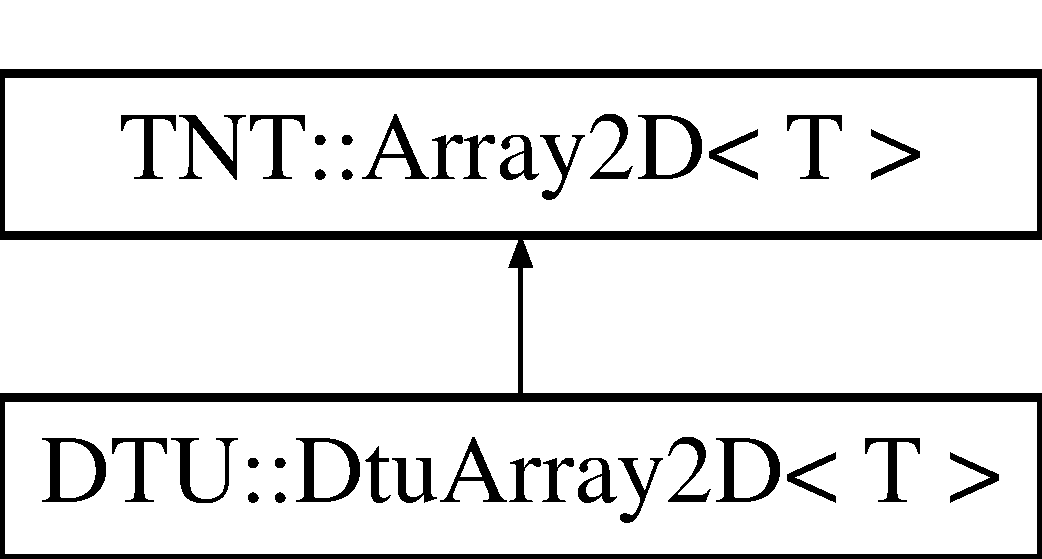
\includegraphics[height=2.000000cm]{classTNT_1_1Array2D}
\end{center}
\end{figure}
\subsection*{Public Types}
\begin{DoxyCompactItemize}
\item 
typedef T \hyperlink{classTNT_1_1Array2D_a4b8dd8e113fb40e26d44bc2f7a45cb44}{value\-\_\-type}
\end{DoxyCompactItemize}
\subsection*{Public Member Functions}
\begin{DoxyCompactItemize}
\item 
\hyperlink{classTNT_1_1Array2D_ab01d5e4b88c04d9e4906e7ea069f9dc0}{Array2\-D} ()
\item 
\hyperlink{classTNT_1_1Array2D_a80990fd85f6c04956a247d43d23a6af4}{Array2\-D} (int m, int n)
\item 
\hyperlink{classTNT_1_1Array2D_a7447ecfb709ce78db3c78ff21104f6f2}{Array2\-D} (int m, int n, T $\ast$a)
\item 
\hyperlink{classTNT_1_1Array2D_a0bbed4288ef81ee0c9baabf69c824191}{Array2\-D} (int m, int n, const T \&a)
\item 
\hyperlink{classTNT_1_1Array2D_a065e795f6f2486ca7ea0bca09200dbd4}{Array2\-D} (const \hyperlink{classTNT_1_1Array2D}{Array2\-D} \&A)
\item 
\hyperlink{classTNT_1_1Array2D_a4049d0d72eddf918ec9a84f799b92e47}{operator T $\ast$$\ast$} ()
\item 
\hyperlink{classTNT_1_1Array2D_a38bf24494047929cb39c89b5c9c516f7}{operator const T $\ast$$\ast$} ()
\item 
\hyperlink{classTNT_1_1Array2D}{Array2\-D} \& \hyperlink{classTNT_1_1Array2D_af14c53b4b3977ab8ecb34da61e5a6e4c}{operator=} (const T \&a)
\item 
\hyperlink{classTNT_1_1Array2D}{Array2\-D} \& \hyperlink{classTNT_1_1Array2D_a291213171560381b270246be0bbe75c0}{operator=} (const \hyperlink{classTNT_1_1Array2D}{Array2\-D} \&A)
\item 
\hyperlink{classTNT_1_1Array2D}{Array2\-D} \& \hyperlink{classTNT_1_1Array2D_a45629cdcb71db56e68c61721ebd6e1cf}{ref} (const \hyperlink{classTNT_1_1Array2D}{Array2\-D} \&A)
\item 
\hyperlink{classTNT_1_1Array2D}{Array2\-D} \hyperlink{classTNT_1_1Array2D_a475f33af47a33135fde05d1e01fdf0c3}{copy} () const 
\item 
\hyperlink{classTNT_1_1Array2D}{Array2\-D} \& \hyperlink{classTNT_1_1Array2D_a24f86f6bf4fd6436946c82e55a12af24}{inject} (const \hyperlink{classTNT_1_1Array2D}{Array2\-D} \&A)
\item 
T $\ast$ \hyperlink{classTNT_1_1Array2D_a472e0ff84ff7767033dc847a7a9c34cd}{operator\mbox{[}$\,$\mbox{]}} (int i)
\item 
const T $\ast$ \hyperlink{classTNT_1_1Array2D_a780cb44fafeec22f9ec591062e370ae1}{operator\mbox{[}$\,$\mbox{]}} (int i) const 
\item 
int \hyperlink{classTNT_1_1Array2D_a3997cd7973cd903cc46c0bd7abde03c0}{dim1} () const 
\item 
int \hyperlink{classTNT_1_1Array2D_a6efd5ac98f02bb42340be1d5cbf4c9c1}{dim2} () const 
\item 
\hyperlink{classTNT_1_1Array2D_a87c0133fa83755104b75631cfa4d6ab7}{$\sim$\-Array2\-D} ()
\item 
int \hyperlink{classTNT_1_1Array2D_a1669732a1a744a212c0c23b0cbafb1f1}{ref\-\_\-count} ()
\item 
int \hyperlink{classTNT_1_1Array2D_adb80c979d57de1fc4422a683703027b9}{ref\-\_\-count\-\_\-data} ()
\item 
int \hyperlink{classTNT_1_1Array2D_a8f4e8eca39d733e01642f35df5b4484b}{ref\-\_\-count\-\_\-dim1} ()
\item 
\hyperlink{classTNT_1_1Array2D}{Array2\-D} \hyperlink{classTNT_1_1Array2D_accf36569414a2570497d2a3f9fe68f52}{subarray} (int i0, int i1, int j0, int j1)
\end{DoxyCompactItemize}
\subsection*{Protected Attributes}
\begin{DoxyCompactItemize}
\item 
\hyperlink{classTNT_1_1Array1D}{Array1\-D}$<$ T $>$ \hyperlink{classTNT_1_1Array2D_afb5d79a6c51d8d27121a982aaff4bc47}{data\-\_\-}
\item 
\hyperlink{classTNT_1_1Array1D}{Array1\-D}$<$ T $\ast$ $>$ \hyperlink{classTNT_1_1Array2D_ad270c8e9b65bb9ae37fcf05797b17cbf}{v\-\_\-}
\item 
int \hyperlink{classTNT_1_1Array2D_ad866fbd5cb16df751ebf9e4eea6f2f22}{m\-\_\-}
\item 
int \hyperlink{classTNT_1_1Array2D_a4a182694802765bdb358f9737ab922b1}{n\-\_\-}
\end{DoxyCompactItemize}


\subsection{Member Typedef Documentation}
\hypertarget{classTNT_1_1Array2D_a4b8dd8e113fb40e26d44bc2f7a45cb44}{\index{T\-N\-T\-::\-Array2\-D@{T\-N\-T\-::\-Array2\-D}!value\-\_\-type@{value\-\_\-type}}
\index{value\-\_\-type@{value\-\_\-type}!TNT::Array2D@{T\-N\-T\-::\-Array2\-D}}
\subsubsection[{value\-\_\-type}]{\setlength{\rightskip}{0pt plus 5cm}template$<$class T$>$ typedef T {\bf T\-N\-T\-::\-Array2\-D}$<$ T $>$\-::{\bf value\-\_\-type}}}\label{classTNT_1_1Array2D_a4b8dd8e113fb40e26d44bc2f7a45cb44}


\subsection{Constructor \& Destructor Documentation}
\hypertarget{classTNT_1_1Array2D_ab01d5e4b88c04d9e4906e7ea069f9dc0}{\index{T\-N\-T\-::\-Array2\-D@{T\-N\-T\-::\-Array2\-D}!Array2\-D@{Array2\-D}}
\index{Array2\-D@{Array2\-D}!TNT::Array2D@{T\-N\-T\-::\-Array2\-D}}
\subsubsection[{Array2\-D}]{\setlength{\rightskip}{0pt plus 5cm}template$<$class T $>$ {\bf T\-N\-T\-::\-Array2\-D}$<$ T $>$\-::{\bf Array2\-D} (
\begin{DoxyParamCaption}
{}
\end{DoxyParamCaption}
)}}\label{classTNT_1_1Array2D_ab01d5e4b88c04d9e4906e7ea069f9dc0}
\hypertarget{classTNT_1_1Array2D_a80990fd85f6c04956a247d43d23a6af4}{\index{T\-N\-T\-::\-Array2\-D@{T\-N\-T\-::\-Array2\-D}!Array2\-D@{Array2\-D}}
\index{Array2\-D@{Array2\-D}!TNT::Array2D@{T\-N\-T\-::\-Array2\-D}}
\subsubsection[{Array2\-D}]{\setlength{\rightskip}{0pt plus 5cm}template$<$class T $>$ {\bf T\-N\-T\-::\-Array2\-D}$<$ T $>$\-::{\bf Array2\-D} (
\begin{DoxyParamCaption}
\item[{int}]{m, }
\item[{int}]{n}
\end{DoxyParamCaption}
)}}\label{classTNT_1_1Array2D_a80990fd85f6c04956a247d43d23a6af4}
\hypertarget{classTNT_1_1Array2D_a7447ecfb709ce78db3c78ff21104f6f2}{\index{T\-N\-T\-::\-Array2\-D@{T\-N\-T\-::\-Array2\-D}!Array2\-D@{Array2\-D}}
\index{Array2\-D@{Array2\-D}!TNT::Array2D@{T\-N\-T\-::\-Array2\-D}}
\subsubsection[{Array2\-D}]{\setlength{\rightskip}{0pt plus 5cm}template$<$class T$>$ {\bf T\-N\-T\-::\-Array2\-D}$<$ T $>$\-::{\bf Array2\-D} (
\begin{DoxyParamCaption}
\item[{int}]{m, }
\item[{int}]{n, }
\item[{T $\ast$}]{a}
\end{DoxyParamCaption}
)}}\label{classTNT_1_1Array2D_a7447ecfb709ce78db3c78ff21104f6f2}
\hypertarget{classTNT_1_1Array2D_a0bbed4288ef81ee0c9baabf69c824191}{\index{T\-N\-T\-::\-Array2\-D@{T\-N\-T\-::\-Array2\-D}!Array2\-D@{Array2\-D}}
\index{Array2\-D@{Array2\-D}!TNT::Array2D@{T\-N\-T\-::\-Array2\-D}}
\subsubsection[{Array2\-D}]{\setlength{\rightskip}{0pt plus 5cm}template$<$class T$>$ {\bf T\-N\-T\-::\-Array2\-D}$<$ T $>$\-::{\bf Array2\-D} (
\begin{DoxyParamCaption}
\item[{int}]{m, }
\item[{int}]{n, }
\item[{const T \&}]{a}
\end{DoxyParamCaption}
)}}\label{classTNT_1_1Array2D_a0bbed4288ef81ee0c9baabf69c824191}
\hypertarget{classTNT_1_1Array2D_a065e795f6f2486ca7ea0bca09200dbd4}{\index{T\-N\-T\-::\-Array2\-D@{T\-N\-T\-::\-Array2\-D}!Array2\-D@{Array2\-D}}
\index{Array2\-D@{Array2\-D}!TNT::Array2D@{T\-N\-T\-::\-Array2\-D}}
\subsubsection[{Array2\-D}]{\setlength{\rightskip}{0pt plus 5cm}template$<$class T$>$ {\bf T\-N\-T\-::\-Array2\-D}$<$ T $>$\-::{\bf Array2\-D} (
\begin{DoxyParamCaption}
\item[{const {\bf Array2\-D}$<$ T $>$ \&}]{A}
\end{DoxyParamCaption}
)\hspace{0.3cm}{\ttfamily [inline]}}}\label{classTNT_1_1Array2D_a065e795f6f2486ca7ea0bca09200dbd4}
\hypertarget{classTNT_1_1Array2D_a87c0133fa83755104b75631cfa4d6ab7}{\index{T\-N\-T\-::\-Array2\-D@{T\-N\-T\-::\-Array2\-D}!$\sim$\-Array2\-D@{$\sim$\-Array2\-D}}
\index{$\sim$\-Array2\-D@{$\sim$\-Array2\-D}!TNT::Array2D@{T\-N\-T\-::\-Array2\-D}}
\subsubsection[{$\sim$\-Array2\-D}]{\setlength{\rightskip}{0pt plus 5cm}template$<$class T $>$ {\bf T\-N\-T\-::\-Array2\-D}$<$ T $>$\-::$\sim${\bf Array2\-D} (
\begin{DoxyParamCaption}
{}
\end{DoxyParamCaption}
)}}\label{classTNT_1_1Array2D_a87c0133fa83755104b75631cfa4d6ab7}


\subsection{Member Function Documentation}
\hypertarget{classTNT_1_1Array2D_a475f33af47a33135fde05d1e01fdf0c3}{\index{T\-N\-T\-::\-Array2\-D@{T\-N\-T\-::\-Array2\-D}!copy@{copy}}
\index{copy@{copy}!TNT::Array2D@{T\-N\-T\-::\-Array2\-D}}
\subsubsection[{copy}]{\setlength{\rightskip}{0pt plus 5cm}template$<$class T $>$ {\bf Array2\-D}$<$ T $>$ {\bf T\-N\-T\-::\-Array2\-D}$<$ T $>$\-::copy (
\begin{DoxyParamCaption}
{}
\end{DoxyParamCaption}
) const}}\label{classTNT_1_1Array2D_a475f33af47a33135fde05d1e01fdf0c3}
\hypertarget{classTNT_1_1Array2D_a3997cd7973cd903cc46c0bd7abde03c0}{\index{T\-N\-T\-::\-Array2\-D@{T\-N\-T\-::\-Array2\-D}!dim1@{dim1}}
\index{dim1@{dim1}!TNT::Array2D@{T\-N\-T\-::\-Array2\-D}}
\subsubsection[{dim1}]{\setlength{\rightskip}{0pt plus 5cm}template$<$class T $>$ int {\bf T\-N\-T\-::\-Array2\-D}$<$ T $>$\-::dim1 (
\begin{DoxyParamCaption}
{}
\end{DoxyParamCaption}
) const\hspace{0.3cm}{\ttfamily [inline]}}}\label{classTNT_1_1Array2D_a3997cd7973cd903cc46c0bd7abde03c0}
\hypertarget{classTNT_1_1Array2D_a6efd5ac98f02bb42340be1d5cbf4c9c1}{\index{T\-N\-T\-::\-Array2\-D@{T\-N\-T\-::\-Array2\-D}!dim2@{dim2}}
\index{dim2@{dim2}!TNT::Array2D@{T\-N\-T\-::\-Array2\-D}}
\subsubsection[{dim2}]{\setlength{\rightskip}{0pt plus 5cm}template$<$class T $>$ int {\bf T\-N\-T\-::\-Array2\-D}$<$ T $>$\-::dim2 (
\begin{DoxyParamCaption}
{}
\end{DoxyParamCaption}
) const\hspace{0.3cm}{\ttfamily [inline]}}}\label{classTNT_1_1Array2D_a6efd5ac98f02bb42340be1d5cbf4c9c1}
\hypertarget{classTNT_1_1Array2D_a24f86f6bf4fd6436946c82e55a12af24}{\index{T\-N\-T\-::\-Array2\-D@{T\-N\-T\-::\-Array2\-D}!inject@{inject}}
\index{inject@{inject}!TNT::Array2D@{T\-N\-T\-::\-Array2\-D}}
\subsubsection[{inject}]{\setlength{\rightskip}{0pt plus 5cm}template$<$class T $>$ {\bf Array2\-D}$<$ T $>$ \& {\bf T\-N\-T\-::\-Array2\-D}$<$ T $>$\-::inject (
\begin{DoxyParamCaption}
\item[{const {\bf Array2\-D}$<$ T $>$ \&}]{A}
\end{DoxyParamCaption}
)}}\label{classTNT_1_1Array2D_a24f86f6bf4fd6436946c82e55a12af24}
\hypertarget{classTNT_1_1Array2D_a38bf24494047929cb39c89b5c9c516f7}{\index{T\-N\-T\-::\-Array2\-D@{T\-N\-T\-::\-Array2\-D}!operator const T $\ast$$\ast$@{operator const T $\ast$$\ast$}}
\index{operator const T $\ast$$\ast$@{operator const T $\ast$$\ast$}!TNT::Array2D@{T\-N\-T\-::\-Array2\-D}}
\subsubsection[{operator const T $\ast$$\ast$}]{\setlength{\rightskip}{0pt plus 5cm}template$<$class T $>$ {\bf T\-N\-T\-::\-Array2\-D}$<$ T $>$\-::operator const T $\ast$$\ast$ (
\begin{DoxyParamCaption}
{}
\end{DoxyParamCaption}
)\hspace{0.3cm}{\ttfamily [inline]}}}\label{classTNT_1_1Array2D_a38bf24494047929cb39c89b5c9c516f7}
\hypertarget{classTNT_1_1Array2D_a4049d0d72eddf918ec9a84f799b92e47}{\index{T\-N\-T\-::\-Array2\-D@{T\-N\-T\-::\-Array2\-D}!operator T $\ast$$\ast$@{operator T $\ast$$\ast$}}
\index{operator T $\ast$$\ast$@{operator T $\ast$$\ast$}!TNT::Array2D@{T\-N\-T\-::\-Array2\-D}}
\subsubsection[{operator T $\ast$$\ast$}]{\setlength{\rightskip}{0pt plus 5cm}template$<$class T $>$ {\bf T\-N\-T\-::\-Array2\-D}$<$ T $>$\-::operator T $\ast$$\ast$ (
\begin{DoxyParamCaption}
{}
\end{DoxyParamCaption}
)\hspace{0.3cm}{\ttfamily [inline]}}}\label{classTNT_1_1Array2D_a4049d0d72eddf918ec9a84f799b92e47}
\hypertarget{classTNT_1_1Array2D_af14c53b4b3977ab8ecb34da61e5a6e4c}{\index{T\-N\-T\-::\-Array2\-D@{T\-N\-T\-::\-Array2\-D}!operator=@{operator=}}
\index{operator=@{operator=}!TNT::Array2D@{T\-N\-T\-::\-Array2\-D}}
\subsubsection[{operator=}]{\setlength{\rightskip}{0pt plus 5cm}template$<$class T$>$ {\bf Array2\-D}$<$ T $>$ \& {\bf T\-N\-T\-::\-Array2\-D}$<$ T $>$\-::operator= (
\begin{DoxyParamCaption}
\item[{const T \&}]{a}
\end{DoxyParamCaption}
)\hspace{0.3cm}{\ttfamily [inline]}}}\label{classTNT_1_1Array2D_af14c53b4b3977ab8ecb34da61e5a6e4c}
\hypertarget{classTNT_1_1Array2D_a291213171560381b270246be0bbe75c0}{\index{T\-N\-T\-::\-Array2\-D@{T\-N\-T\-::\-Array2\-D}!operator=@{operator=}}
\index{operator=@{operator=}!TNT::Array2D@{T\-N\-T\-::\-Array2\-D}}
\subsubsection[{operator=}]{\setlength{\rightskip}{0pt plus 5cm}template$<$class T$>$ {\bf Array2\-D}$<$ T $>$ \& {\bf T\-N\-T\-::\-Array2\-D}$<$ T $>$\-::operator= (
\begin{DoxyParamCaption}
\item[{const {\bf Array2\-D}$<$ T $>$ \&}]{A}
\end{DoxyParamCaption}
)\hspace{0.3cm}{\ttfamily [inline]}}}\label{classTNT_1_1Array2D_a291213171560381b270246be0bbe75c0}
\hypertarget{classTNT_1_1Array2D_a472e0ff84ff7767033dc847a7a9c34cd}{\index{T\-N\-T\-::\-Array2\-D@{T\-N\-T\-::\-Array2\-D}!operator\mbox{[}$\,$\mbox{]}@{operator[]}}
\index{operator\mbox{[}$\,$\mbox{]}@{operator[]}!TNT::Array2D@{T\-N\-T\-::\-Array2\-D}}
\subsubsection[{operator[]}]{\setlength{\rightskip}{0pt plus 5cm}template$<$class T $>$ T $\ast$ {\bf T\-N\-T\-::\-Array2\-D}$<$ T $>$\-::operator\mbox{[}$\,$\mbox{]} (
\begin{DoxyParamCaption}
\item[{int}]{i}
\end{DoxyParamCaption}
)\hspace{0.3cm}{\ttfamily [inline]}}}\label{classTNT_1_1Array2D_a472e0ff84ff7767033dc847a7a9c34cd}
\hypertarget{classTNT_1_1Array2D_a780cb44fafeec22f9ec591062e370ae1}{\index{T\-N\-T\-::\-Array2\-D@{T\-N\-T\-::\-Array2\-D}!operator\mbox{[}$\,$\mbox{]}@{operator[]}}
\index{operator\mbox{[}$\,$\mbox{]}@{operator[]}!TNT::Array2D@{T\-N\-T\-::\-Array2\-D}}
\subsubsection[{operator[]}]{\setlength{\rightskip}{0pt plus 5cm}template$<$class T $>$ const T $\ast$ {\bf T\-N\-T\-::\-Array2\-D}$<$ T $>$\-::operator\mbox{[}$\,$\mbox{]} (
\begin{DoxyParamCaption}
\item[{int}]{i}
\end{DoxyParamCaption}
) const\hspace{0.3cm}{\ttfamily [inline]}}}\label{classTNT_1_1Array2D_a780cb44fafeec22f9ec591062e370ae1}
\hypertarget{classTNT_1_1Array2D_a45629cdcb71db56e68c61721ebd6e1cf}{\index{T\-N\-T\-::\-Array2\-D@{T\-N\-T\-::\-Array2\-D}!ref@{ref}}
\index{ref@{ref}!TNT::Array2D@{T\-N\-T\-::\-Array2\-D}}
\subsubsection[{ref}]{\setlength{\rightskip}{0pt plus 5cm}template$<$class T $>$ {\bf Array2\-D}$<$ T $>$ \& {\bf T\-N\-T\-::\-Array2\-D}$<$ T $>$\-::ref (
\begin{DoxyParamCaption}
\item[{const {\bf Array2\-D}$<$ T $>$ \&}]{A}
\end{DoxyParamCaption}
)\hspace{0.3cm}{\ttfamily [inline]}}}\label{classTNT_1_1Array2D_a45629cdcb71db56e68c61721ebd6e1cf}
\hypertarget{classTNT_1_1Array2D_a1669732a1a744a212c0c23b0cbafb1f1}{\index{T\-N\-T\-::\-Array2\-D@{T\-N\-T\-::\-Array2\-D}!ref\-\_\-count@{ref\-\_\-count}}
\index{ref\-\_\-count@{ref\-\_\-count}!TNT::Array2D@{T\-N\-T\-::\-Array2\-D}}
\subsubsection[{ref\-\_\-count}]{\setlength{\rightskip}{0pt plus 5cm}template$<$class T $>$ int {\bf T\-N\-T\-::\-Array2\-D}$<$ T $>$\-::ref\-\_\-count (
\begin{DoxyParamCaption}
{}
\end{DoxyParamCaption}
)\hspace{0.3cm}{\ttfamily [inline]}}}\label{classTNT_1_1Array2D_a1669732a1a744a212c0c23b0cbafb1f1}
\hypertarget{classTNT_1_1Array2D_adb80c979d57de1fc4422a683703027b9}{\index{T\-N\-T\-::\-Array2\-D@{T\-N\-T\-::\-Array2\-D}!ref\-\_\-count\-\_\-data@{ref\-\_\-count\-\_\-data}}
\index{ref\-\_\-count\-\_\-data@{ref\-\_\-count\-\_\-data}!TNT::Array2D@{T\-N\-T\-::\-Array2\-D}}
\subsubsection[{ref\-\_\-count\-\_\-data}]{\setlength{\rightskip}{0pt plus 5cm}template$<$class T $>$ int {\bf T\-N\-T\-::\-Array2\-D}$<$ T $>$\-::ref\-\_\-count\-\_\-data (
\begin{DoxyParamCaption}
{}
\end{DoxyParamCaption}
)\hspace{0.3cm}{\ttfamily [inline]}}}\label{classTNT_1_1Array2D_adb80c979d57de1fc4422a683703027b9}
\hypertarget{classTNT_1_1Array2D_a8f4e8eca39d733e01642f35df5b4484b}{\index{T\-N\-T\-::\-Array2\-D@{T\-N\-T\-::\-Array2\-D}!ref\-\_\-count\-\_\-dim1@{ref\-\_\-count\-\_\-dim1}}
\index{ref\-\_\-count\-\_\-dim1@{ref\-\_\-count\-\_\-dim1}!TNT::Array2D@{T\-N\-T\-::\-Array2\-D}}
\subsubsection[{ref\-\_\-count\-\_\-dim1}]{\setlength{\rightskip}{0pt plus 5cm}template$<$class T $>$ int {\bf T\-N\-T\-::\-Array2\-D}$<$ T $>$\-::ref\-\_\-count\-\_\-dim1 (
\begin{DoxyParamCaption}
{}
\end{DoxyParamCaption}
)\hspace{0.3cm}{\ttfamily [inline]}}}\label{classTNT_1_1Array2D_a8f4e8eca39d733e01642f35df5b4484b}
\hypertarget{classTNT_1_1Array2D_accf36569414a2570497d2a3f9fe68f52}{\index{T\-N\-T\-::\-Array2\-D@{T\-N\-T\-::\-Array2\-D}!subarray@{subarray}}
\index{subarray@{subarray}!TNT::Array2D@{T\-N\-T\-::\-Array2\-D}}
\subsubsection[{subarray}]{\setlength{\rightskip}{0pt plus 5cm}template$<$class T $>$ {\bf Array2\-D}$<$ T $>$ {\bf T\-N\-T\-::\-Array2\-D}$<$ T $>$\-::subarray (
\begin{DoxyParamCaption}
\item[{int}]{i0, }
\item[{int}]{i1, }
\item[{int}]{j0, }
\item[{int}]{j1}
\end{DoxyParamCaption}
)}}\label{classTNT_1_1Array2D_accf36569414a2570497d2a3f9fe68f52}
Create a new view to a subarray defined by the boundaries \mbox{[}i0\mbox{]}\mbox{[}i0\mbox{]} and \mbox{[}i1\mbox{]}\mbox{[}j1\mbox{]}. The size of the subarray is (i1-\/i0) by (j1-\/j0). If either of these lengths are zero or negative, the subarray view is null. 

\subsection{Member Data Documentation}
\hypertarget{classTNT_1_1Array2D_afb5d79a6c51d8d27121a982aaff4bc47}{\index{T\-N\-T\-::\-Array2\-D@{T\-N\-T\-::\-Array2\-D}!data\-\_\-@{data\-\_\-}}
\index{data\-\_\-@{data\-\_\-}!TNT::Array2D@{T\-N\-T\-::\-Array2\-D}}
\subsubsection[{data\-\_\-}]{\setlength{\rightskip}{0pt plus 5cm}template$<$class T$>$ {\bf Array1\-D}$<$T$>$ {\bf T\-N\-T\-::\-Array2\-D}$<$ T $>$\-::data\-\_\-\hspace{0.3cm}{\ttfamily [protected]}}}\label{classTNT_1_1Array2D_afb5d79a6c51d8d27121a982aaff4bc47}
\hypertarget{classTNT_1_1Array2D_ad866fbd5cb16df751ebf9e4eea6f2f22}{\index{T\-N\-T\-::\-Array2\-D@{T\-N\-T\-::\-Array2\-D}!m\-\_\-@{m\-\_\-}}
\index{m\-\_\-@{m\-\_\-}!TNT::Array2D@{T\-N\-T\-::\-Array2\-D}}
\subsubsection[{m\-\_\-}]{\setlength{\rightskip}{0pt plus 5cm}template$<$class T$>$ int {\bf T\-N\-T\-::\-Array2\-D}$<$ T $>$\-::m\-\_\-\hspace{0.3cm}{\ttfamily [protected]}}}\label{classTNT_1_1Array2D_ad866fbd5cb16df751ebf9e4eea6f2f22}
\hypertarget{classTNT_1_1Array2D_a4a182694802765bdb358f9737ab922b1}{\index{T\-N\-T\-::\-Array2\-D@{T\-N\-T\-::\-Array2\-D}!n\-\_\-@{n\-\_\-}}
\index{n\-\_\-@{n\-\_\-}!TNT::Array2D@{T\-N\-T\-::\-Array2\-D}}
\subsubsection[{n\-\_\-}]{\setlength{\rightskip}{0pt plus 5cm}template$<$class T$>$ int {\bf T\-N\-T\-::\-Array2\-D}$<$ T $>$\-::n\-\_\-\hspace{0.3cm}{\ttfamily [protected]}}}\label{classTNT_1_1Array2D_a4a182694802765bdb358f9737ab922b1}
\hypertarget{classTNT_1_1Array2D_ad270c8e9b65bb9ae37fcf05797b17cbf}{\index{T\-N\-T\-::\-Array2\-D@{T\-N\-T\-::\-Array2\-D}!v\-\_\-@{v\-\_\-}}
\index{v\-\_\-@{v\-\_\-}!TNT::Array2D@{T\-N\-T\-::\-Array2\-D}}
\subsubsection[{v\-\_\-}]{\setlength{\rightskip}{0pt plus 5cm}template$<$class T$>$ {\bf Array1\-D}$<$T$\ast$$>$ {\bf T\-N\-T\-::\-Array2\-D}$<$ T $>$\-::v\-\_\-\hspace{0.3cm}{\ttfamily [protected]}}}\label{classTNT_1_1Array2D_ad270c8e9b65bb9ae37fcf05797b17cbf}


The documentation for this class was generated from the following file\-:\begin{DoxyCompactItemize}
\item 
/media/philipjhj/\-Data/\-One\-Drive/\-Studie/\-Studenterprogrammør/\-S\-B\-S3/smartphonebrainscanner2-\/core/src/jama125/\hyperlink{tnt__array2d_8h}{tnt\-\_\-array2d.\-h}\end{DoxyCompactItemize}

\hypertarget{classTNT_1_1Array3D}{\section{T\-N\-T\-:\-:Array3\-D$<$ T $>$ Class Template Reference}
\label{classTNT_1_1Array3D}\index{T\-N\-T\-::\-Array3\-D$<$ T $>$@{T\-N\-T\-::\-Array3\-D$<$ T $>$}}
}


{\ttfamily \#include $<$tnt\-\_\-array3d.\-h$>$}

\subsection*{Public Types}
\begin{DoxyCompactItemize}
\item 
typedef T \hyperlink{classTNT_1_1Array3D_a51945370abf416e829e6a50bdb0af6d5}{value\-\_\-type}
\end{DoxyCompactItemize}
\subsection*{Public Member Functions}
\begin{DoxyCompactItemize}
\item 
\hyperlink{classTNT_1_1Array3D_a94ceeeadc5904e9ec4069ef61394ff8e}{Array3\-D} ()
\item 
\hyperlink{classTNT_1_1Array3D_a3556263018d605d22ce74699f3898559}{Array3\-D} (int m, int n, int g)
\item 
\hyperlink{classTNT_1_1Array3D_a3e5d89a3999c39540a441aeebcd8edc4}{Array3\-D} (int m, int n, int g, T val)
\item 
\hyperlink{classTNT_1_1Array3D_a5830c3a1275b2498bdceb6502e63c28f}{Array3\-D} (int m, int n, int g, T $\ast$a)
\item 
\hyperlink{classTNT_1_1Array3D_a35b7704b6c061b4150d64592650ba83f}{operator T $\ast$$\ast$$\ast$} ()
\item 
\hyperlink{classTNT_1_1Array3D_a420ffed5ca81952d989afe406450a9b0}{operator const T $\ast$$\ast$$\ast$} ()
\item 
\hyperlink{classTNT_1_1Array3D_ae137326853df4e4cdcc52afff3f5d85a}{Array3\-D} (const \hyperlink{classTNT_1_1Array3D}{Array3\-D} \&A)
\item 
\hyperlink{classTNT_1_1Array3D}{Array3\-D} \& \hyperlink{classTNT_1_1Array3D_a405e5c9c24c7b3895533fa8f870f9bfd}{operator=} (const T \&a)
\item 
\hyperlink{classTNT_1_1Array3D}{Array3\-D} \& \hyperlink{classTNT_1_1Array3D_a13fa6cf87fcfc5847972569f325f9b56}{operator=} (const \hyperlink{classTNT_1_1Array3D}{Array3\-D} \&A)
\item 
\hyperlink{classTNT_1_1Array3D}{Array3\-D} \& \hyperlink{classTNT_1_1Array3D_aded40455c8a0b48c3c3d0688ea90180a}{ref} (const \hyperlink{classTNT_1_1Array3D}{Array3\-D} \&A)
\item 
\hyperlink{classTNT_1_1Array3D}{Array3\-D} \hyperlink{classTNT_1_1Array3D_abef414d4382ab6cac80bb32a53f8db55}{copy} () const 
\item 
\hyperlink{classTNT_1_1Array3D}{Array3\-D} \& \hyperlink{classTNT_1_1Array3D_ac9004a4cc385cbfc0d3b742efd605e1c}{inject} (const \hyperlink{classTNT_1_1Array3D}{Array3\-D} \&A)
\item 
T $\ast$$\ast$ \hyperlink{classTNT_1_1Array3D_aea9175ed3125b3061f3be0db72656518}{operator\mbox{[}$\,$\mbox{]}} (int i)
\item 
const T $\ast$const $\ast$ \hyperlink{classTNT_1_1Array3D_ad5587fca33f70c1b3b3f421fc5087c25}{operator\mbox{[}$\,$\mbox{]}} (int i) const 
\item 
int \hyperlink{classTNT_1_1Array3D_ad75b16e73207a349a9a996659c338296}{dim1} () const 
\item 
int \hyperlink{classTNT_1_1Array3D_a458595e0b81ebbc1b193b4b737defd00}{dim2} () const 
\item 
int \hyperlink{classTNT_1_1Array3D_a0f147ed03d878ed375e21ef8a00af483}{dim3} () const 
\item 
\hyperlink{classTNT_1_1Array3D_af22e1bc22155dc84168ae00f5f26258b}{$\sim$\-Array3\-D} ()
\item 
int \hyperlink{classTNT_1_1Array3D_a50bbefb0aa842c2d7208b67fb09bb0d9}{ref\-\_\-count} ()
\item 
\hyperlink{classTNT_1_1Array3D}{Array3\-D} \hyperlink{classTNT_1_1Array3D_a365b3f6c5eb41e5189b20b25d80aee98}{subarray} (int i0, int i1, int j0, int j1, int k0, int k1)
\end{DoxyCompactItemize}


\subsection{Member Typedef Documentation}
\hypertarget{classTNT_1_1Array3D_a51945370abf416e829e6a50bdb0af6d5}{\index{T\-N\-T\-::\-Array3\-D@{T\-N\-T\-::\-Array3\-D}!value\-\_\-type@{value\-\_\-type}}
\index{value\-\_\-type@{value\-\_\-type}!TNT::Array3D@{T\-N\-T\-::\-Array3\-D}}
\subsubsection[{value\-\_\-type}]{\setlength{\rightskip}{0pt plus 5cm}template$<$class T$>$ typedef T {\bf T\-N\-T\-::\-Array3\-D}$<$ T $>$\-::{\bf value\-\_\-type}}}\label{classTNT_1_1Array3D_a51945370abf416e829e6a50bdb0af6d5}


\subsection{Constructor \& Destructor Documentation}
\hypertarget{classTNT_1_1Array3D_a94ceeeadc5904e9ec4069ef61394ff8e}{\index{T\-N\-T\-::\-Array3\-D@{T\-N\-T\-::\-Array3\-D}!Array3\-D@{Array3\-D}}
\index{Array3\-D@{Array3\-D}!TNT::Array3D@{T\-N\-T\-::\-Array3\-D}}
\subsubsection[{Array3\-D}]{\setlength{\rightskip}{0pt plus 5cm}template$<$class T $>$ {\bf T\-N\-T\-::\-Array3\-D}$<$ T $>$\-::{\bf Array3\-D} (
\begin{DoxyParamCaption}
{}
\end{DoxyParamCaption}
)}}\label{classTNT_1_1Array3D_a94ceeeadc5904e9ec4069ef61394ff8e}
\hypertarget{classTNT_1_1Array3D_a3556263018d605d22ce74699f3898559}{\index{T\-N\-T\-::\-Array3\-D@{T\-N\-T\-::\-Array3\-D}!Array3\-D@{Array3\-D}}
\index{Array3\-D@{Array3\-D}!TNT::Array3D@{T\-N\-T\-::\-Array3\-D}}
\subsubsection[{Array3\-D}]{\setlength{\rightskip}{0pt plus 5cm}template$<$class T $>$ {\bf T\-N\-T\-::\-Array3\-D}$<$ T $>$\-::{\bf Array3\-D} (
\begin{DoxyParamCaption}
\item[{int}]{m, }
\item[{int}]{n, }
\item[{int}]{g}
\end{DoxyParamCaption}
)}}\label{classTNT_1_1Array3D_a3556263018d605d22ce74699f3898559}
\hypertarget{classTNT_1_1Array3D_a3e5d89a3999c39540a441aeebcd8edc4}{\index{T\-N\-T\-::\-Array3\-D@{T\-N\-T\-::\-Array3\-D}!Array3\-D@{Array3\-D}}
\index{Array3\-D@{Array3\-D}!TNT::Array3D@{T\-N\-T\-::\-Array3\-D}}
\subsubsection[{Array3\-D}]{\setlength{\rightskip}{0pt plus 5cm}template$<$class T $>$ {\bf T\-N\-T\-::\-Array3\-D}$<$ T $>$\-::{\bf Array3\-D} (
\begin{DoxyParamCaption}
\item[{int}]{m, }
\item[{int}]{n, }
\item[{int}]{g, }
\item[{T}]{val}
\end{DoxyParamCaption}
)}}\label{classTNT_1_1Array3D_a3e5d89a3999c39540a441aeebcd8edc4}
\hypertarget{classTNT_1_1Array3D_a5830c3a1275b2498bdceb6502e63c28f}{\index{T\-N\-T\-::\-Array3\-D@{T\-N\-T\-::\-Array3\-D}!Array3\-D@{Array3\-D}}
\index{Array3\-D@{Array3\-D}!TNT::Array3D@{T\-N\-T\-::\-Array3\-D}}
\subsubsection[{Array3\-D}]{\setlength{\rightskip}{0pt plus 5cm}template$<$class T $>$ {\bf T\-N\-T\-::\-Array3\-D}$<$ T $>$\-::{\bf Array3\-D} (
\begin{DoxyParamCaption}
\item[{int}]{m, }
\item[{int}]{n, }
\item[{int}]{g, }
\item[{T $\ast$}]{a}
\end{DoxyParamCaption}
)}}\label{classTNT_1_1Array3D_a5830c3a1275b2498bdceb6502e63c28f}
\hypertarget{classTNT_1_1Array3D_ae137326853df4e4cdcc52afff3f5d85a}{\index{T\-N\-T\-::\-Array3\-D@{T\-N\-T\-::\-Array3\-D}!Array3\-D@{Array3\-D}}
\index{Array3\-D@{Array3\-D}!TNT::Array3D@{T\-N\-T\-::\-Array3\-D}}
\subsubsection[{Array3\-D}]{\setlength{\rightskip}{0pt plus 5cm}template$<$class T $>$ {\bf T\-N\-T\-::\-Array3\-D}$<$ T $>$\-::{\bf Array3\-D} (
\begin{DoxyParamCaption}
\item[{const {\bf Array3\-D}$<$ T $>$ \&}]{A}
\end{DoxyParamCaption}
)\hspace{0.3cm}{\ttfamily [inline]}}}\label{classTNT_1_1Array3D_ae137326853df4e4cdcc52afff3f5d85a}
\hypertarget{classTNT_1_1Array3D_af22e1bc22155dc84168ae00f5f26258b}{\index{T\-N\-T\-::\-Array3\-D@{T\-N\-T\-::\-Array3\-D}!$\sim$\-Array3\-D@{$\sim$\-Array3\-D}}
\index{$\sim$\-Array3\-D@{$\sim$\-Array3\-D}!TNT::Array3D@{T\-N\-T\-::\-Array3\-D}}
\subsubsection[{$\sim$\-Array3\-D}]{\setlength{\rightskip}{0pt plus 5cm}template$<$class T $>$ {\bf T\-N\-T\-::\-Array3\-D}$<$ T $>$\-::$\sim${\bf Array3\-D} (
\begin{DoxyParamCaption}
{}
\end{DoxyParamCaption}
)}}\label{classTNT_1_1Array3D_af22e1bc22155dc84168ae00f5f26258b}


\subsection{Member Function Documentation}
\hypertarget{classTNT_1_1Array3D_abef414d4382ab6cac80bb32a53f8db55}{\index{T\-N\-T\-::\-Array3\-D@{T\-N\-T\-::\-Array3\-D}!copy@{copy}}
\index{copy@{copy}!TNT::Array3D@{T\-N\-T\-::\-Array3\-D}}
\subsubsection[{copy}]{\setlength{\rightskip}{0pt plus 5cm}template$<$class T $>$ {\bf Array3\-D}$<$ T $>$ {\bf T\-N\-T\-::\-Array3\-D}$<$ T $>$\-::copy (
\begin{DoxyParamCaption}
{}
\end{DoxyParamCaption}
) const}}\label{classTNT_1_1Array3D_abef414d4382ab6cac80bb32a53f8db55}
\hypertarget{classTNT_1_1Array3D_ad75b16e73207a349a9a996659c338296}{\index{T\-N\-T\-::\-Array3\-D@{T\-N\-T\-::\-Array3\-D}!dim1@{dim1}}
\index{dim1@{dim1}!TNT::Array3D@{T\-N\-T\-::\-Array3\-D}}
\subsubsection[{dim1}]{\setlength{\rightskip}{0pt plus 5cm}template$<$class T $>$ int {\bf T\-N\-T\-::\-Array3\-D}$<$ T $>$\-::dim1 (
\begin{DoxyParamCaption}
{}
\end{DoxyParamCaption}
) const\hspace{0.3cm}{\ttfamily [inline]}}}\label{classTNT_1_1Array3D_ad75b16e73207a349a9a996659c338296}
\hypertarget{classTNT_1_1Array3D_a458595e0b81ebbc1b193b4b737defd00}{\index{T\-N\-T\-::\-Array3\-D@{T\-N\-T\-::\-Array3\-D}!dim2@{dim2}}
\index{dim2@{dim2}!TNT::Array3D@{T\-N\-T\-::\-Array3\-D}}
\subsubsection[{dim2}]{\setlength{\rightskip}{0pt plus 5cm}template$<$class T $>$ int {\bf T\-N\-T\-::\-Array3\-D}$<$ T $>$\-::dim2 (
\begin{DoxyParamCaption}
{}
\end{DoxyParamCaption}
) const\hspace{0.3cm}{\ttfamily [inline]}}}\label{classTNT_1_1Array3D_a458595e0b81ebbc1b193b4b737defd00}
\hypertarget{classTNT_1_1Array3D_a0f147ed03d878ed375e21ef8a00af483}{\index{T\-N\-T\-::\-Array3\-D@{T\-N\-T\-::\-Array3\-D}!dim3@{dim3}}
\index{dim3@{dim3}!TNT::Array3D@{T\-N\-T\-::\-Array3\-D}}
\subsubsection[{dim3}]{\setlength{\rightskip}{0pt plus 5cm}template$<$class T $>$ int {\bf T\-N\-T\-::\-Array3\-D}$<$ T $>$\-::dim3 (
\begin{DoxyParamCaption}
{}
\end{DoxyParamCaption}
) const\hspace{0.3cm}{\ttfamily [inline]}}}\label{classTNT_1_1Array3D_a0f147ed03d878ed375e21ef8a00af483}
\hypertarget{classTNT_1_1Array3D_ac9004a4cc385cbfc0d3b742efd605e1c}{\index{T\-N\-T\-::\-Array3\-D@{T\-N\-T\-::\-Array3\-D}!inject@{inject}}
\index{inject@{inject}!TNT::Array3D@{T\-N\-T\-::\-Array3\-D}}
\subsubsection[{inject}]{\setlength{\rightskip}{0pt plus 5cm}template$<$class T $>$ {\bf Array3\-D}$<$ T $>$ \& {\bf T\-N\-T\-::\-Array3\-D}$<$ T $>$\-::inject (
\begin{DoxyParamCaption}
\item[{const {\bf Array3\-D}$<$ T $>$ \&}]{A}
\end{DoxyParamCaption}
)}}\label{classTNT_1_1Array3D_ac9004a4cc385cbfc0d3b742efd605e1c}
\hypertarget{classTNT_1_1Array3D_a420ffed5ca81952d989afe406450a9b0}{\index{T\-N\-T\-::\-Array3\-D@{T\-N\-T\-::\-Array3\-D}!operator const T $\ast$$\ast$$\ast$@{operator const T $\ast$$\ast$$\ast$}}
\index{operator const T $\ast$$\ast$$\ast$@{operator const T $\ast$$\ast$$\ast$}!TNT::Array3D@{T\-N\-T\-::\-Array3\-D}}
\subsubsection[{operator const T $\ast$$\ast$$\ast$}]{\setlength{\rightskip}{0pt plus 5cm}template$<$class T $>$ {\bf T\-N\-T\-::\-Array3\-D}$<$ T $>$\-::operator const T $\ast$$\ast$$\ast$ (
\begin{DoxyParamCaption}
{}
\end{DoxyParamCaption}
)\hspace{0.3cm}{\ttfamily [inline]}}}\label{classTNT_1_1Array3D_a420ffed5ca81952d989afe406450a9b0}
\hypertarget{classTNT_1_1Array3D_a35b7704b6c061b4150d64592650ba83f}{\index{T\-N\-T\-::\-Array3\-D@{T\-N\-T\-::\-Array3\-D}!operator T $\ast$$\ast$$\ast$@{operator T $\ast$$\ast$$\ast$}}
\index{operator T $\ast$$\ast$$\ast$@{operator T $\ast$$\ast$$\ast$}!TNT::Array3D@{T\-N\-T\-::\-Array3\-D}}
\subsubsection[{operator T $\ast$$\ast$$\ast$}]{\setlength{\rightskip}{0pt plus 5cm}template$<$class T $>$ {\bf T\-N\-T\-::\-Array3\-D}$<$ T $>$\-::operator T $\ast$$\ast$$\ast$ (
\begin{DoxyParamCaption}
{}
\end{DoxyParamCaption}
)\hspace{0.3cm}{\ttfamily [inline]}}}\label{classTNT_1_1Array3D_a35b7704b6c061b4150d64592650ba83f}
\hypertarget{classTNT_1_1Array3D_a405e5c9c24c7b3895533fa8f870f9bfd}{\index{T\-N\-T\-::\-Array3\-D@{T\-N\-T\-::\-Array3\-D}!operator=@{operator=}}
\index{operator=@{operator=}!TNT::Array3D@{T\-N\-T\-::\-Array3\-D}}
\subsubsection[{operator=}]{\setlength{\rightskip}{0pt plus 5cm}template$<$class T $>$ {\bf Array3\-D}$<$ T $>$ \& {\bf T\-N\-T\-::\-Array3\-D}$<$ T $>$\-::operator= (
\begin{DoxyParamCaption}
\item[{const T \&}]{a}
\end{DoxyParamCaption}
)\hspace{0.3cm}{\ttfamily [inline]}}}\label{classTNT_1_1Array3D_a405e5c9c24c7b3895533fa8f870f9bfd}
\hypertarget{classTNT_1_1Array3D_a13fa6cf87fcfc5847972569f325f9b56}{\index{T\-N\-T\-::\-Array3\-D@{T\-N\-T\-::\-Array3\-D}!operator=@{operator=}}
\index{operator=@{operator=}!TNT::Array3D@{T\-N\-T\-::\-Array3\-D}}
\subsubsection[{operator=}]{\setlength{\rightskip}{0pt plus 5cm}template$<$class T $>$ {\bf Array3\-D}$<$ T $>$ \& {\bf T\-N\-T\-::\-Array3\-D}$<$ T $>$\-::operator= (
\begin{DoxyParamCaption}
\item[{const {\bf Array3\-D}$<$ T $>$ \&}]{A}
\end{DoxyParamCaption}
)\hspace{0.3cm}{\ttfamily [inline]}}}\label{classTNT_1_1Array3D_a13fa6cf87fcfc5847972569f325f9b56}
\hypertarget{classTNT_1_1Array3D_aea9175ed3125b3061f3be0db72656518}{\index{T\-N\-T\-::\-Array3\-D@{T\-N\-T\-::\-Array3\-D}!operator\mbox{[}$\,$\mbox{]}@{operator[]}}
\index{operator\mbox{[}$\,$\mbox{]}@{operator[]}!TNT::Array3D@{T\-N\-T\-::\-Array3\-D}}
\subsubsection[{operator[]}]{\setlength{\rightskip}{0pt plus 5cm}template$<$class T $>$ T $\ast$$\ast$ {\bf T\-N\-T\-::\-Array3\-D}$<$ T $>$\-::operator\mbox{[}$\,$\mbox{]} (
\begin{DoxyParamCaption}
\item[{int}]{i}
\end{DoxyParamCaption}
)\hspace{0.3cm}{\ttfamily [inline]}}}\label{classTNT_1_1Array3D_aea9175ed3125b3061f3be0db72656518}
\hypertarget{classTNT_1_1Array3D_ad5587fca33f70c1b3b3f421fc5087c25}{\index{T\-N\-T\-::\-Array3\-D@{T\-N\-T\-::\-Array3\-D}!operator\mbox{[}$\,$\mbox{]}@{operator[]}}
\index{operator\mbox{[}$\,$\mbox{]}@{operator[]}!TNT::Array3D@{T\-N\-T\-::\-Array3\-D}}
\subsubsection[{operator[]}]{\setlength{\rightskip}{0pt plus 5cm}template$<$class T $>$ const T $\ast$const $\ast$ {\bf T\-N\-T\-::\-Array3\-D}$<$ T $>$\-::operator\mbox{[}$\,$\mbox{]} (
\begin{DoxyParamCaption}
\item[{int}]{i}
\end{DoxyParamCaption}
) const\hspace{0.3cm}{\ttfamily [inline]}}}\label{classTNT_1_1Array3D_ad5587fca33f70c1b3b3f421fc5087c25}
\hypertarget{classTNT_1_1Array3D_aded40455c8a0b48c3c3d0688ea90180a}{\index{T\-N\-T\-::\-Array3\-D@{T\-N\-T\-::\-Array3\-D}!ref@{ref}}
\index{ref@{ref}!TNT::Array3D@{T\-N\-T\-::\-Array3\-D}}
\subsubsection[{ref}]{\setlength{\rightskip}{0pt plus 5cm}template$<$class T $>$ {\bf Array3\-D}$<$ T $>$ \& {\bf T\-N\-T\-::\-Array3\-D}$<$ T $>$\-::ref (
\begin{DoxyParamCaption}
\item[{const {\bf Array3\-D}$<$ T $>$ \&}]{A}
\end{DoxyParamCaption}
)\hspace{0.3cm}{\ttfamily [inline]}}}\label{classTNT_1_1Array3D_aded40455c8a0b48c3c3d0688ea90180a}
\hypertarget{classTNT_1_1Array3D_a50bbefb0aa842c2d7208b67fb09bb0d9}{\index{T\-N\-T\-::\-Array3\-D@{T\-N\-T\-::\-Array3\-D}!ref\-\_\-count@{ref\-\_\-count}}
\index{ref\-\_\-count@{ref\-\_\-count}!TNT::Array3D@{T\-N\-T\-::\-Array3\-D}}
\subsubsection[{ref\-\_\-count}]{\setlength{\rightskip}{0pt plus 5cm}template$<$class T$>$ int {\bf T\-N\-T\-::\-Array3\-D}$<$ T $>$\-::ref\-\_\-count (
\begin{DoxyParamCaption}
{}
\end{DoxyParamCaption}
)\hspace{0.3cm}{\ttfamily [inline]}}}\label{classTNT_1_1Array3D_a50bbefb0aa842c2d7208b67fb09bb0d9}
\hypertarget{classTNT_1_1Array3D_a365b3f6c5eb41e5189b20b25d80aee98}{\index{T\-N\-T\-::\-Array3\-D@{T\-N\-T\-::\-Array3\-D}!subarray@{subarray}}
\index{subarray@{subarray}!TNT::Array3D@{T\-N\-T\-::\-Array3\-D}}
\subsubsection[{subarray}]{\setlength{\rightskip}{0pt plus 5cm}template$<$class T $>$ {\bf Array3\-D}$<$ T $>$ {\bf T\-N\-T\-::\-Array3\-D}$<$ T $>$\-::subarray (
\begin{DoxyParamCaption}
\item[{int}]{i0, }
\item[{int}]{i1, }
\item[{int}]{j0, }
\item[{int}]{j1, }
\item[{int}]{k0, }
\item[{int}]{k1}
\end{DoxyParamCaption}
)}}\label{classTNT_1_1Array3D_a365b3f6c5eb41e5189b20b25d80aee98}


The documentation for this class was generated from the following file\-:\begin{DoxyCompactItemize}
\item 
/media/philipjhj/\-Data/\-One\-Drive/\-Studie/\-Studenterprogrammør/\-S\-B\-S3/smartphonebrainscanner2-\/core/src/jama125/\hyperlink{tnt__array3d_8h}{tnt\-\_\-array3d.\-h}\end{DoxyCompactItemize}

\hypertarget{classJAMA_1_1Cholesky}{\section{J\-A\-M\-A\-:\-:Cholesky$<$ Real $>$ Class Template Reference}
\label{classJAMA_1_1Cholesky}\index{J\-A\-M\-A\-::\-Cholesky$<$ Real $>$@{J\-A\-M\-A\-::\-Cholesky$<$ Real $>$}}
}


{\ttfamily \#include $<$jama\-\_\-cholesky.\-h$>$}

\subsection*{Public Member Functions}
\begin{DoxyCompactItemize}
\item 
\hyperlink{classJAMA_1_1Cholesky_a0af68661b83b7a6be938b42e2b2591b6}{Cholesky} ()
\item 
\hyperlink{classJAMA_1_1Cholesky_af859c41220c4313470d28fa13706ff63}{Cholesky} (const \hyperlink{classTNT_1_1Array2D}{Array2\-D}$<$ Real $>$ \&A)
\item 
\hyperlink{classTNT_1_1Array2D}{Array2\-D}$<$ Real $>$ \hyperlink{classJAMA_1_1Cholesky_a274b8bbd584bcf84ec860a24aa2b8b2a}{get\-L} () const 
\item 
\hyperlink{classTNT_1_1Array1D}{Array1\-D}$<$ Real $>$ \hyperlink{classJAMA_1_1Cholesky_af0f727e2b0e989f7606cdb49de69f119}{solve} (const \hyperlink{classTNT_1_1Array1D}{Array1\-D}$<$ Real $>$ \&B)
\item 
\hyperlink{classTNT_1_1Array2D}{Array2\-D}$<$ Real $>$ \hyperlink{classJAMA_1_1Cholesky_a8a3c0067663955146713a9aa3b8a3413}{solve} (const \hyperlink{classTNT_1_1Array2D}{Array2\-D}$<$ Real $>$ \&B)
\item 
int \hyperlink{classJAMA_1_1Cholesky_ab8ac7d6f0c9ef4e0fb74b001fe03ff90}{is\-\_\-spd} () const 
\end{DoxyCompactItemize}


\subsection{Detailed Description}
\subsubsection*{template$<$class Real$>$class J\-A\-M\-A\-::\-Cholesky$<$ Real $>$}

For a symmetric, positive definite matrix A, this function computes the \hyperlink{classJAMA_1_1Cholesky}{Cholesky} factorization, i.\-e. it computes a lower triangular matrix L such that A = L$\ast$\-L'. If the matrix is not symmetric or positive definite, the function computes only a partial decomposition. This can be tested with the \hyperlink{classJAMA_1_1Cholesky_ab8ac7d6f0c9ef4e0fb74b001fe03ff90}{is\-\_\-spd()} flag.

Typical usage looks like\-: 
\begin{DoxyPre}
 \hyperlink{classTNT_1_1Array2D}{Array2D<double>} A(n,n);
 \hyperlink{classTNT_1_1Array2D}{Array2D<double>} L;\end{DoxyPre}



\begin{DoxyPre}  ...\end{DoxyPre}



\begin{DoxyPre} Cholesky<double> chol(A);\end{DoxyPre}



\begin{DoxyPre} if (chol.is\_spd())
    L = chol.getL();\end{DoxyPre}



\begin{DoxyPre} else
    cout << "factorization was not complete.\(\backslash\)n";\end{DoxyPre}



\begin{DoxyPre} \end{DoxyPre}


(Adapted from \hyperlink{namespaceJAMA}{J\-A\-M\-A}, a Java Matrix Library, developed by jointly by the Mathworks and N\-I\-S\-T; see \href{http://math.nist.gov/javanumerics/jama}{\tt http\-://math.\-nist.\-gov/javanumerics/jama}). 

\subsection{Constructor \& Destructor Documentation}
\hypertarget{classJAMA_1_1Cholesky_a0af68661b83b7a6be938b42e2b2591b6}{\index{J\-A\-M\-A\-::\-Cholesky@{J\-A\-M\-A\-::\-Cholesky}!Cholesky@{Cholesky}}
\index{Cholesky@{Cholesky}!JAMA::Cholesky@{J\-A\-M\-A\-::\-Cholesky}}
\subsubsection[{Cholesky}]{\setlength{\rightskip}{0pt plus 5cm}template$<$class Real $>$ {\bf J\-A\-M\-A\-::\-Cholesky}$<$ Real $>$\-::{\bf Cholesky} (
\begin{DoxyParamCaption}
{}
\end{DoxyParamCaption}
)}}\label{classJAMA_1_1Cholesky_a0af68661b83b7a6be938b42e2b2591b6}
\hypertarget{classJAMA_1_1Cholesky_af859c41220c4313470d28fa13706ff63}{\index{J\-A\-M\-A\-::\-Cholesky@{J\-A\-M\-A\-::\-Cholesky}!Cholesky@{Cholesky}}
\index{Cholesky@{Cholesky}!JAMA::Cholesky@{J\-A\-M\-A\-::\-Cholesky}}
\subsubsection[{Cholesky}]{\setlength{\rightskip}{0pt plus 5cm}template$<$class Real $>$ {\bf J\-A\-M\-A\-::\-Cholesky}$<$ Real $>$\-::{\bf Cholesky} (
\begin{DoxyParamCaption}
\item[{const {\bf Array2\-D}$<$ Real $>$ \&}]{A}
\end{DoxyParamCaption}
)}}\label{classJAMA_1_1Cholesky_af859c41220c4313470d28fa13706ff63}
Constructs a lower triangular matrix L, such that L$\ast$\-L'= A. If A is not symmetric positive-\/definite (S\-P\-D), only a partial factorization is performed. If \hyperlink{classJAMA_1_1Cholesky_ab8ac7d6f0c9ef4e0fb74b001fe03ff90}{is\-\_\-spd()} evalutate true (1) then the factorizaiton was successful. 

\subsection{Member Function Documentation}
\hypertarget{classJAMA_1_1Cholesky_a274b8bbd584bcf84ec860a24aa2b8b2a}{\index{J\-A\-M\-A\-::\-Cholesky@{J\-A\-M\-A\-::\-Cholesky}!get\-L@{get\-L}}
\index{get\-L@{get\-L}!JAMA::Cholesky@{J\-A\-M\-A\-::\-Cholesky}}
\subsubsection[{get\-L}]{\setlength{\rightskip}{0pt plus 5cm}template$<$class Real $>$ {\bf Array2\-D}$<$ Real $>$ {\bf J\-A\-M\-A\-::\-Cholesky}$<$ Real $>$\-::get\-L (
\begin{DoxyParamCaption}
{}
\end{DoxyParamCaption}
) const}}\label{classJAMA_1_1Cholesky_a274b8bbd584bcf84ec860a24aa2b8b2a}
\begin{DoxyReturn}{Returns}
the lower triangular factor, L, such that L$\ast$\-L'=A. 
\end{DoxyReturn}
\hypertarget{classJAMA_1_1Cholesky_ab8ac7d6f0c9ef4e0fb74b001fe03ff90}{\index{J\-A\-M\-A\-::\-Cholesky@{J\-A\-M\-A\-::\-Cholesky}!is\-\_\-spd@{is\-\_\-spd}}
\index{is\-\_\-spd@{is\-\_\-spd}!JAMA::Cholesky@{J\-A\-M\-A\-::\-Cholesky}}
\subsubsection[{is\-\_\-spd}]{\setlength{\rightskip}{0pt plus 5cm}template$<$class Real $>$ int {\bf J\-A\-M\-A\-::\-Cholesky}$<$ Real $>$\-::is\-\_\-spd (
\begin{DoxyParamCaption}
{}
\end{DoxyParamCaption}
) const}}\label{classJAMA_1_1Cholesky_ab8ac7d6f0c9ef4e0fb74b001fe03ff90}
\begin{DoxyReturn}{Returns}
1, if original matrix to be factored was symmetric positive-\/definite (S\-P\-D). 
\end{DoxyReturn}
\hypertarget{classJAMA_1_1Cholesky_af0f727e2b0e989f7606cdb49de69f119}{\index{J\-A\-M\-A\-::\-Cholesky@{J\-A\-M\-A\-::\-Cholesky}!solve@{solve}}
\index{solve@{solve}!JAMA::Cholesky@{J\-A\-M\-A\-::\-Cholesky}}
\subsubsection[{solve}]{\setlength{\rightskip}{0pt plus 5cm}template$<$class Real $>$ {\bf Array1\-D}$<$ Real $>$ {\bf J\-A\-M\-A\-::\-Cholesky}$<$ Real $>$\-::solve (
\begin{DoxyParamCaption}
\item[{const {\bf Array1\-D}$<$ Real $>$ \&}]{b}
\end{DoxyParamCaption}
)}}\label{classJAMA_1_1Cholesky_af0f727e2b0e989f7606cdb49de69f119}
Solve a linear system A$\ast$x = b, using the previously computed cholesky factorization of A\-: L$\ast$\-L'.


\begin{DoxyParams}{Parameters}
{\em B} & A Matrix with as many rows as A and any number of columns. \\
\hline
\end{DoxyParams}
\begin{DoxyReturn}{Returns}
x so that L$\ast$\-L'$\ast$x = b. If b is nonconformat, or if A was not symmetric posidtive definite, a null (0x0) array is returned. 
\end{DoxyReturn}
\hypertarget{classJAMA_1_1Cholesky_a8a3c0067663955146713a9aa3b8a3413}{\index{J\-A\-M\-A\-::\-Cholesky@{J\-A\-M\-A\-::\-Cholesky}!solve@{solve}}
\index{solve@{solve}!JAMA::Cholesky@{J\-A\-M\-A\-::\-Cholesky}}
\subsubsection[{solve}]{\setlength{\rightskip}{0pt plus 5cm}template$<$class Real $>$ {\bf Array2\-D}$<$ Real $>$ {\bf J\-A\-M\-A\-::\-Cholesky}$<$ Real $>$\-::solve (
\begin{DoxyParamCaption}
\item[{const {\bf Array2\-D}$<$ Real $>$ \&}]{B}
\end{DoxyParamCaption}
)}}\label{classJAMA_1_1Cholesky_a8a3c0067663955146713a9aa3b8a3413}
Solve a linear system A$\ast$\-X = B, using the previously computed cholesky factorization of A\-: L$\ast$\-L'.


\begin{DoxyParams}{Parameters}
{\em B} & A Matrix with as many rows as A and any number of columns. \\
\hline
\end{DoxyParams}
\begin{DoxyReturn}{Returns}
X so that L$\ast$\-L'$\ast$\-X = B. If B is nonconformat, or if A was not symmetric posidtive definite, a null (0x0) array is returned. 
\end{DoxyReturn}


The documentation for this class was generated from the following file\-:\begin{DoxyCompactItemize}
\item 
/media/philipjhj/\-Data/\-One\-Drive/\-Studie/\-Studenterprogrammør/\-S\-B\-S3/smartphonebrainscanner2-\/core/src/jama125/\hyperlink{jama__cholesky_8h}{jama\-\_\-cholesky.\-h}\end{DoxyCompactItemize}

\hypertarget{classClass}{\section{Class Class Reference}
\label{classClass}\index{Class@{Class}}
}


\subsection{Detailed Description}
reading the raw data from the device and delivering single well formed packet.

Smartphone Brain Scanner 2 License Agreement (M\-I\-T License)

Copyright (c) 2012 Arkadiusz Stopczynski, Jakob Eg Larsen, Carsten Stahlhut, Michael Kai Petersen, Lars Kai Hansen. Technical University of Denmark, \hyperlink{namespaceDTU}{D\-T\-U} Informatics, Cognitive Systems Section. \href{http://code.google.com/p/smartphonebrainscanner2}{\tt http\-://code.\-google.\-com/p/smartphonebrainscanner2}

Permission is hereby granted, free of charge, to any person obtaining a copy of this software and associated documentation files (the \char`\"{}\-Software\char`\"{}), to deal in the Software without restriction, including without limitation the rights to use, copy, modify, merge, publish, distribute, sublicense, and/or sell copies of the Software, and to permit persons to whom the Software is furnished to do so, subject to the following conditions\-:

The above copyright notice and this permission notice shall be included in all copies or substantial portions of the Software.

T\-H\-E S\-O\-F\-T\-W\-A\-R\-E I\-S P\-R\-O\-V\-I\-D\-E\-D \char`\"{}\-A\-S I\-S\char`\"{}, W\-I\-T\-H\-O\-U\-T W\-A\-R\-R\-A\-N\-T\-Y O\-F A\-N\-Y K\-I\-N\-D, E\-X\-P\-R\-E\-S\-S O\-R I\-M\-P\-L\-I\-E\-D, I\-N\-C\-L\-U\-D\-I\-N\-G B\-U\-T N\-O\-T L\-I\-M\-I\-T\-E\-D T\-O T\-H\-E W\-A\-R\-R\-A\-N\-T\-I\-E\-S O\-F M\-E\-R\-C\-H\-A\-N\-T\-A\-B\-I\-L\-I\-T\-Y, F\-I\-T\-N\-E\-S\-S F\-O\-R A P\-A\-R\-T\-I\-C\-U\-L\-A\-R P\-U\-R\-P\-O\-S\-E A\-N\-D N\-O\-N\-I\-N\-F\-R\-I\-N\-G\-E\-M\-E\-N\-T. I\-N N\-O E\-V\-E\-N\-T S\-H\-A\-L\-L T\-H\-E A\-U\-T\-H\-O\-R\-S O\-R C\-O\-P\-Y\-R\-I\-G\-H\-T H\-O\-L\-D\-E\-R\-S B\-E L\-I\-A\-B\-L\-E F\-O\-R A\-N\-Y C\-L\-A\-I\-M, D\-A\-M\-A\-G\-E\-S O\-R O\-T\-H\-E\-R L\-I\-A\-B\-I\-L\-I\-T\-Y, W\-H\-E\-T\-H\-E\-R I\-N A\-N A\-C\-T\-I\-O\-N O\-F C\-O\-N\-T\-R\-A\-C\-T, T\-O\-R\-T O\-R O\-T\-H\-E\-R\-W\-I\-S\-E, A\-R\-I\-S\-I\-N\-G F\-R\-O\-M, O\-U\-T O\-F O\-R I\-N C\-O\-N\-N\-E\-C\-T\-I\-O\-N W\-I\-T\-H T\-H\-E S\-O\-F\-T\-W\-A\-R\-E O\-R T\-H\-E U\-S\-E O\-R O\-T\-H\-E\-R D\-E\-A\-L\-I\-N\-G\-S I\-N T\-H\-E S\-O\-F\-T\-W\-A\-R\-E. \begin{DoxyRefDesc}{Todo}
\item[\hyperlink{todo__todo000001}{Todo}]Meta data as Q\-Map. \end{DoxyRefDesc}
and metadata (such as counters, signal quality, gyro). Certain number of empty packets is constructed in the buffer and then continuosly updated.

Smartphone Brain Scanner 2 License Agreement (M\-I\-T License)

Copyright (c) 2012 Arkadiusz Stopczynski, Jakob Eg Larsen, Carsten Stahlhut, Michael Kai Petersen, Lars Kai Hansen. Technical University of Denmark, \hyperlink{namespaceDTU}{D\-T\-U} Informatics, Cognitive Systems Section. \href{http://code.google.com/p/smartphonebrainscanner2}{\tt http\-://code.\-google.\-com/p/smartphonebrainscanner2}

Permission is hereby granted, free of charge, to any person obtaining a copy of this software and associated documentation files (the \char`\"{}\-Software\char`\"{}), to deal in the Software without restriction, including without limitation the rights to use, copy, modify, merge, publish, distribute, sublicense, and/or sell copies of the Software, and to permit persons to whom the Software is furnished to do so, subject to the following conditions\-:

The above copyright notice and this permission notice shall be included in all copies or substantial portions of the Software.

T\-H\-E S\-O\-F\-T\-W\-A\-R\-E I\-S P\-R\-O\-V\-I\-D\-E\-D \char`\"{}\-A\-S I\-S\char`\"{}, W\-I\-T\-H\-O\-U\-T W\-A\-R\-R\-A\-N\-T\-Y O\-F A\-N\-Y K\-I\-N\-D, E\-X\-P\-R\-E\-S\-S O\-R I\-M\-P\-L\-I\-E\-D, I\-N\-C\-L\-U\-D\-I\-N\-G B\-U\-T N\-O\-T L\-I\-M\-I\-T\-E\-D T\-O T\-H\-E W\-A\-R\-R\-A\-N\-T\-I\-E\-S O\-F M\-E\-R\-C\-H\-A\-N\-T\-A\-B\-I\-L\-I\-T\-Y, F\-I\-T\-N\-E\-S\-S F\-O\-R A P\-A\-R\-T\-I\-C\-U\-L\-A\-R P\-U\-R\-P\-O\-S\-E A\-N\-D N\-O\-N\-I\-N\-F\-R\-I\-N\-G\-E\-M\-E\-N\-T. I\-N N\-O E\-V\-E\-N\-T S\-H\-A\-L\-L T\-H\-E A\-U\-T\-H\-O\-R\-S O\-R C\-O\-P\-Y\-R\-I\-G\-H\-T H\-O\-L\-D\-E\-R\-S B\-E L\-I\-A\-B\-L\-E F\-O\-R A\-N\-Y C\-L\-A\-I\-M, D\-A\-M\-A\-G\-E\-S O\-R O\-T\-H\-E\-R L\-I\-A\-B\-I\-L\-I\-T\-Y, W\-H\-E\-T\-H\-E\-R I\-N A\-N A\-C\-T\-I\-O\-N O\-F C\-O\-N\-T\-R\-A\-C\-T, T\-O\-R\-T O\-R O\-T\-H\-E\-R\-W\-I\-S\-E, A\-R\-I\-S\-I\-N\-G F\-R\-O\-M, O\-U\-T O\-F O\-R I\-N C\-O\-N\-N\-E\-C\-T\-I\-O\-N W\-I\-T\-H T\-H\-E S\-O\-F\-T\-W\-A\-R\-E O\-R T\-H\-E U\-S\-E O\-R O\-T\-H\-E\-R D\-E\-A\-L\-I\-N\-G\-S I\-N T\-H\-E S\-O\-F\-T\-W\-A\-R\-E. \begin{DoxyRefDesc}{Todo}
\item[\hyperlink{todo__todo000003}{Todo}]Filter should be a container for particular implementations of the filter, either static or adaptive. \end{DoxyRefDesc}
temporal filter. 

The documentation for this class was generated from the following file\-:\begin{DoxyCompactItemize}
\item 
/media/philipjhj/\-Data/\-One\-Drive/\-Studie/\-Studenterprogrammør/\-S\-B\-S3/smartphonebrainscanner2-\/core/src/hardware/\hyperlink{sbs2datareader_8h}{sbs2datareader.\-h}\end{DoxyCompactItemize}

\hypertarget{classCRijndael}{\section{C\-Rijndael Class Reference}
\label{classCRijndael}\index{C\-Rijndael@{C\-Rijndael}}
}


{\ttfamily \#include $<$Rijndael.\-h$>$}

\subsection*{Public Types}
\begin{DoxyCompactItemize}
\item 
enum \{ \hyperlink{classCRijndael_ac1444c814f491f48deb465ef667581d2a45277dc10dfb5fb3b29dd622f2fa95e1}{E\-C\-B} =0, 
\hyperlink{classCRijndael_ac1444c814f491f48deb465ef667581d2a0e8f618dfec3ca34a604ed2ec597b4be}{C\-B\-C} =1, 
\hyperlink{classCRijndael_ac1444c814f491f48deb465ef667581d2aeae0d000ef07f3925d0f8d52f5768f64}{C\-F\-B} =2
 \}
\end{DoxyCompactItemize}
\subsection*{Public Member Functions}
\begin{DoxyCompactItemize}
\item 
\hyperlink{classCRijndael_ac8d9fa05974a5db55a2d358d3a9053d9}{C\-Rijndael} ()
\item 
virtual \hyperlink{classCRijndael_a5546851f5b559f4e6390ded7d0275fe2}{$\sim$\-C\-Rijndael} ()
\item 
void \hyperlink{classCRijndael_a6bb75a9fa43efda9d1de93af7f2fa33f}{Make\-Key} (char const $\ast$key, char const $\ast$chain, int keylength=D\-E\-F\-A\-U\-L\-T\-\_\-\-B\-L\-O\-C\-K\-\_\-\-S\-I\-Z\-E, int block\-Size=D\-E\-F\-A\-U\-L\-T\-\_\-\-B\-L\-O\-C\-K\-\_\-\-S\-I\-Z\-E)
\item 
void \hyperlink{classCRijndael_a09387f9fe5f14a9215e124971024d74a}{Encrypt\-Block} (char const $\ast$in, char $\ast$result)
\item 
void \hyperlink{classCRijndael_aa7f895798f3da4ce102ba0c85e417ed0}{Decrypt\-Block} (char const $\ast$in, char $\ast$result)
\item 
void \hyperlink{classCRijndael_a2eed7961ae006ecbbe7d4db81139d2c0}{Encrypt} (char const $\ast$in, char $\ast$result, size\-\_\-t n, int i\-Mode=\hyperlink{classCRijndael_ac1444c814f491f48deb465ef667581d2a45277dc10dfb5fb3b29dd622f2fa95e1}{E\-C\-B})
\item 
void \hyperlink{classCRijndael_ab897e845d52d1b7a9d9f918300181383}{Decrypt} (char const $\ast$in, char $\ast$result, size\-\_\-t n, int i\-Mode=\hyperlink{classCRijndael_ac1444c814f491f48deb465ef667581d2a45277dc10dfb5fb3b29dd622f2fa95e1}{E\-C\-B})
\item 
int \hyperlink{classCRijndael_a7bd67837a28c50ff22b67a1c63856650}{Get\-Key\-Length} ()
\item 
int \hyperlink{classCRijndael_ab4f96cd740474df6929bdd515abe7395}{Get\-Block\-Size} ()
\item 
int \hyperlink{classCRijndael_a16e1f262a77e108dc3dbc67bf52041b7}{Get\-Rounds} ()
\item 
void \hyperlink{classCRijndael_a8f67681d34a25ba8a920353592ab4b1e}{Reset\-Chain} ()
\end{DoxyCompactItemize}
\subsection*{Static Public Attributes}
\begin{DoxyCompactItemize}
\item 
static char const $\ast$ \hyperlink{classCRijndael_ac00e57b7d923c1a6f3e310203e856c9c}{sm\-\_\-chain0} = \char`\"{}\textbackslash{}0\textbackslash{}0\textbackslash{}0\textbackslash{}0\textbackslash{}0\textbackslash{}0\textbackslash{}0\textbackslash{}0\textbackslash{}0\textbackslash{}0\textbackslash{}0\textbackslash{}0\textbackslash{}0\textbackslash{}0\textbackslash{}0\textbackslash{}0\textbackslash{}0\textbackslash{}0\textbackslash{}0\textbackslash{}0\textbackslash{}0\textbackslash{}0\textbackslash{}0\textbackslash{}0\textbackslash{}0\textbackslash{}0\textbackslash{}0\textbackslash{}0\textbackslash{}0\textbackslash{}0\textbackslash{}0\textbackslash{}0\char`\"{}
\end{DoxyCompactItemize}


\subsection{Member Enumeration Documentation}
\hypertarget{classCRijndael_ac1444c814f491f48deb465ef667581d2}{\subsubsection[{anonymous enum}]{\setlength{\rightskip}{0pt plus 5cm}anonymous enum}}\label{classCRijndael_ac1444c814f491f48deb465ef667581d2}
\begin{Desc}
\item[Enumerator]\par
\begin{description}
\index{E\-C\-B@{E\-C\-B}!C\-Rijndael@{C\-Rijndael}}\index{C\-Rijndael@{C\-Rijndael}!E\-C\-B@{E\-C\-B}}\item[{\em 
\hypertarget{classCRijndael_ac1444c814f491f48deb465ef667581d2a45277dc10dfb5fb3b29dd622f2fa95e1}{E\-C\-B}\label{classCRijndael_ac1444c814f491f48deb465ef667581d2a45277dc10dfb5fb3b29dd622f2fa95e1}
}]\index{C\-B\-C@{C\-B\-C}!C\-Rijndael@{C\-Rijndael}}\index{C\-Rijndael@{C\-Rijndael}!C\-B\-C@{C\-B\-C}}\item[{\em 
\hypertarget{classCRijndael_ac1444c814f491f48deb465ef667581d2a0e8f618dfec3ca34a604ed2ec597b4be}{C\-B\-C}\label{classCRijndael_ac1444c814f491f48deb465ef667581d2a0e8f618dfec3ca34a604ed2ec597b4be}
}]\index{C\-F\-B@{C\-F\-B}!C\-Rijndael@{C\-Rijndael}}\index{C\-Rijndael@{C\-Rijndael}!C\-F\-B@{C\-F\-B}}\item[{\em 
\hypertarget{classCRijndael_ac1444c814f491f48deb465ef667581d2aeae0d000ef07f3925d0f8d52f5768f64}{C\-F\-B}\label{classCRijndael_ac1444c814f491f48deb465ef667581d2aeae0d000ef07f3925d0f8d52f5768f64}
}]\end{description}
\end{Desc}


\subsection{Constructor \& Destructor Documentation}
\hypertarget{classCRijndael_ac8d9fa05974a5db55a2d358d3a9053d9}{\index{C\-Rijndael@{C\-Rijndael}!C\-Rijndael@{C\-Rijndael}}
\index{C\-Rijndael@{C\-Rijndael}!CRijndael@{C\-Rijndael}}
\subsubsection[{C\-Rijndael}]{\setlength{\rightskip}{0pt plus 5cm}C\-Rijndael\-::\-C\-Rijndael (
\begin{DoxyParamCaption}
{}
\end{DoxyParamCaption}
)}}\label{classCRijndael_ac8d9fa05974a5db55a2d358d3a9053d9}
\hypertarget{classCRijndael_a5546851f5b559f4e6390ded7d0275fe2}{\index{C\-Rijndael@{C\-Rijndael}!$\sim$\-C\-Rijndael@{$\sim$\-C\-Rijndael}}
\index{$\sim$\-C\-Rijndael@{$\sim$\-C\-Rijndael}!CRijndael@{C\-Rijndael}}
\subsubsection[{$\sim$\-C\-Rijndael}]{\setlength{\rightskip}{0pt plus 5cm}C\-Rijndael\-::$\sim$\-C\-Rijndael (
\begin{DoxyParamCaption}
{}
\end{DoxyParamCaption}
)\hspace{0.3cm}{\ttfamily [virtual]}}}\label{classCRijndael_a5546851f5b559f4e6390ded7d0275fe2}


\subsection{Member Function Documentation}
\hypertarget{classCRijndael_ab897e845d52d1b7a9d9f918300181383}{\index{C\-Rijndael@{C\-Rijndael}!Decrypt@{Decrypt}}
\index{Decrypt@{Decrypt}!CRijndael@{C\-Rijndael}}
\subsubsection[{Decrypt}]{\setlength{\rightskip}{0pt plus 5cm}void C\-Rijndael\-::\-Decrypt (
\begin{DoxyParamCaption}
\item[{char const $\ast$}]{in, }
\item[{char $\ast$}]{result, }
\item[{size\-\_\-t}]{n, }
\item[{int}]{i\-Mode = {\ttfamily {\bf E\-C\-B}}}
\end{DoxyParamCaption}
)}}\label{classCRijndael_ab897e845d52d1b7a9d9f918300181383}
\hypertarget{classCRijndael_aa7f895798f3da4ce102ba0c85e417ed0}{\index{C\-Rijndael@{C\-Rijndael}!Decrypt\-Block@{Decrypt\-Block}}
\index{Decrypt\-Block@{Decrypt\-Block}!CRijndael@{C\-Rijndael}}
\subsubsection[{Decrypt\-Block}]{\setlength{\rightskip}{0pt plus 5cm}void C\-Rijndael\-::\-Decrypt\-Block (
\begin{DoxyParamCaption}
\item[{char const $\ast$}]{in, }
\item[{char $\ast$}]{result}
\end{DoxyParamCaption}
)}}\label{classCRijndael_aa7f895798f3da4ce102ba0c85e417ed0}
\hypertarget{classCRijndael_a2eed7961ae006ecbbe7d4db81139d2c0}{\index{C\-Rijndael@{C\-Rijndael}!Encrypt@{Encrypt}}
\index{Encrypt@{Encrypt}!CRijndael@{C\-Rijndael}}
\subsubsection[{Encrypt}]{\setlength{\rightskip}{0pt plus 5cm}void C\-Rijndael\-::\-Encrypt (
\begin{DoxyParamCaption}
\item[{char const $\ast$}]{in, }
\item[{char $\ast$}]{result, }
\item[{size\-\_\-t}]{n, }
\item[{int}]{i\-Mode = {\ttfamily {\bf E\-C\-B}}}
\end{DoxyParamCaption}
)}}\label{classCRijndael_a2eed7961ae006ecbbe7d4db81139d2c0}
\hypertarget{classCRijndael_a09387f9fe5f14a9215e124971024d74a}{\index{C\-Rijndael@{C\-Rijndael}!Encrypt\-Block@{Encrypt\-Block}}
\index{Encrypt\-Block@{Encrypt\-Block}!CRijndael@{C\-Rijndael}}
\subsubsection[{Encrypt\-Block}]{\setlength{\rightskip}{0pt plus 5cm}void C\-Rijndael\-::\-Encrypt\-Block (
\begin{DoxyParamCaption}
\item[{char const $\ast$}]{in, }
\item[{char $\ast$}]{result}
\end{DoxyParamCaption}
)}}\label{classCRijndael_a09387f9fe5f14a9215e124971024d74a}
\hypertarget{classCRijndael_ab4f96cd740474df6929bdd515abe7395}{\index{C\-Rijndael@{C\-Rijndael}!Get\-Block\-Size@{Get\-Block\-Size}}
\index{Get\-Block\-Size@{Get\-Block\-Size}!CRijndael@{C\-Rijndael}}
\subsubsection[{Get\-Block\-Size}]{\setlength{\rightskip}{0pt plus 5cm}int C\-Rijndael\-::\-Get\-Block\-Size (
\begin{DoxyParamCaption}
{}
\end{DoxyParamCaption}
)\hspace{0.3cm}{\ttfamily [inline]}}}\label{classCRijndael_ab4f96cd740474df6929bdd515abe7395}
\hypertarget{classCRijndael_a7bd67837a28c50ff22b67a1c63856650}{\index{C\-Rijndael@{C\-Rijndael}!Get\-Key\-Length@{Get\-Key\-Length}}
\index{Get\-Key\-Length@{Get\-Key\-Length}!CRijndael@{C\-Rijndael}}
\subsubsection[{Get\-Key\-Length}]{\setlength{\rightskip}{0pt plus 5cm}int C\-Rijndael\-::\-Get\-Key\-Length (
\begin{DoxyParamCaption}
{}
\end{DoxyParamCaption}
)\hspace{0.3cm}{\ttfamily [inline]}}}\label{classCRijndael_a7bd67837a28c50ff22b67a1c63856650}
\hypertarget{classCRijndael_a16e1f262a77e108dc3dbc67bf52041b7}{\index{C\-Rijndael@{C\-Rijndael}!Get\-Rounds@{Get\-Rounds}}
\index{Get\-Rounds@{Get\-Rounds}!CRijndael@{C\-Rijndael}}
\subsubsection[{Get\-Rounds}]{\setlength{\rightskip}{0pt plus 5cm}int C\-Rijndael\-::\-Get\-Rounds (
\begin{DoxyParamCaption}
{}
\end{DoxyParamCaption}
)\hspace{0.3cm}{\ttfamily [inline]}}}\label{classCRijndael_a16e1f262a77e108dc3dbc67bf52041b7}
\hypertarget{classCRijndael_a6bb75a9fa43efda9d1de93af7f2fa33f}{\index{C\-Rijndael@{C\-Rijndael}!Make\-Key@{Make\-Key}}
\index{Make\-Key@{Make\-Key}!CRijndael@{C\-Rijndael}}
\subsubsection[{Make\-Key}]{\setlength{\rightskip}{0pt plus 5cm}void C\-Rijndael\-::\-Make\-Key (
\begin{DoxyParamCaption}
\item[{char const $\ast$}]{key, }
\item[{char const $\ast$}]{chain, }
\item[{int}]{keylength = {\ttfamily DEFAULT\-\_\-BLOCK\-\_\-SIZE}, }
\item[{int}]{block\-Size = {\ttfamily DEFAULT\-\_\-BLOCK\-\_\-SIZE}}
\end{DoxyParamCaption}
)}}\label{classCRijndael_a6bb75a9fa43efda9d1de93af7f2fa33f}
\hypertarget{classCRijndael_a8f67681d34a25ba8a920353592ab4b1e}{\index{C\-Rijndael@{C\-Rijndael}!Reset\-Chain@{Reset\-Chain}}
\index{Reset\-Chain@{Reset\-Chain}!CRijndael@{C\-Rijndael}}
\subsubsection[{Reset\-Chain}]{\setlength{\rightskip}{0pt plus 5cm}void C\-Rijndael\-::\-Reset\-Chain (
\begin{DoxyParamCaption}
{}
\end{DoxyParamCaption}
)\hspace{0.3cm}{\ttfamily [inline]}}}\label{classCRijndael_a8f67681d34a25ba8a920353592ab4b1e}


\subsection{Member Data Documentation}
\hypertarget{classCRijndael_ac00e57b7d923c1a6f3e310203e856c9c}{\index{C\-Rijndael@{C\-Rijndael}!sm\-\_\-chain0@{sm\-\_\-chain0}}
\index{sm\-\_\-chain0@{sm\-\_\-chain0}!CRijndael@{C\-Rijndael}}
\subsubsection[{sm\-\_\-chain0}]{\setlength{\rightskip}{0pt plus 5cm}char const $\ast$ C\-Rijndael\-::sm\-\_\-chain0 = \char`\"{}\textbackslash{}0\textbackslash{}0\textbackslash{}0\textbackslash{}0\textbackslash{}0\textbackslash{}0\textbackslash{}0\textbackslash{}0\textbackslash{}0\textbackslash{}0\textbackslash{}0\textbackslash{}0\textbackslash{}0\textbackslash{}0\textbackslash{}0\textbackslash{}0\textbackslash{}0\textbackslash{}0\textbackslash{}0\textbackslash{}0\textbackslash{}0\textbackslash{}0\textbackslash{}0\textbackslash{}0\textbackslash{}0\textbackslash{}0\textbackslash{}0\textbackslash{}0\textbackslash{}0\textbackslash{}0\textbackslash{}0\textbackslash{}0\char`\"{}\hspace{0.3cm}{\ttfamily [static]}}}\label{classCRijndael_ac00e57b7d923c1a6f3e310203e856c9c}


The documentation for this class was generated from the following files\-:\begin{DoxyCompactItemize}
\item 
/media/philipjhj/\-Data/\-One\-Drive/\-Studie/\-Studenterprogrammør/\-S\-B\-S3/smartphonebrainscanner2-\/core/src/utils/\hyperlink{Rijndael_8h}{Rijndael.\-h}\item 
/media/philipjhj/\-Data/\-One\-Drive/\-Studie/\-Studenterprogrammør/\-S\-B\-S3/smartphonebrainscanner2-\/core/src/utils/\hyperlink{Rijndael_8cpp}{Rijndael.\-cpp}\end{DoxyCompactItemize}

\hypertarget{classDTU_1_1DtuArray2D}{\section{D\-T\-U\-:\-:Dtu\-Array2\-D$<$ T $>$ Class Template Reference}
\label{classDTU_1_1DtuArray2D}\index{D\-T\-U\-::\-Dtu\-Array2\-D$<$ T $>$@{D\-T\-U\-::\-Dtu\-Array2\-D$<$ T $>$}}
}


{\ttfamily \#include $<$dtu\-\_\-array\-\_\-2d.\-h$>$}

Inheritance diagram for D\-T\-U\-:\-:Dtu\-Array2\-D$<$ T $>$\-:\begin{figure}[H]
\begin{center}
\leavevmode
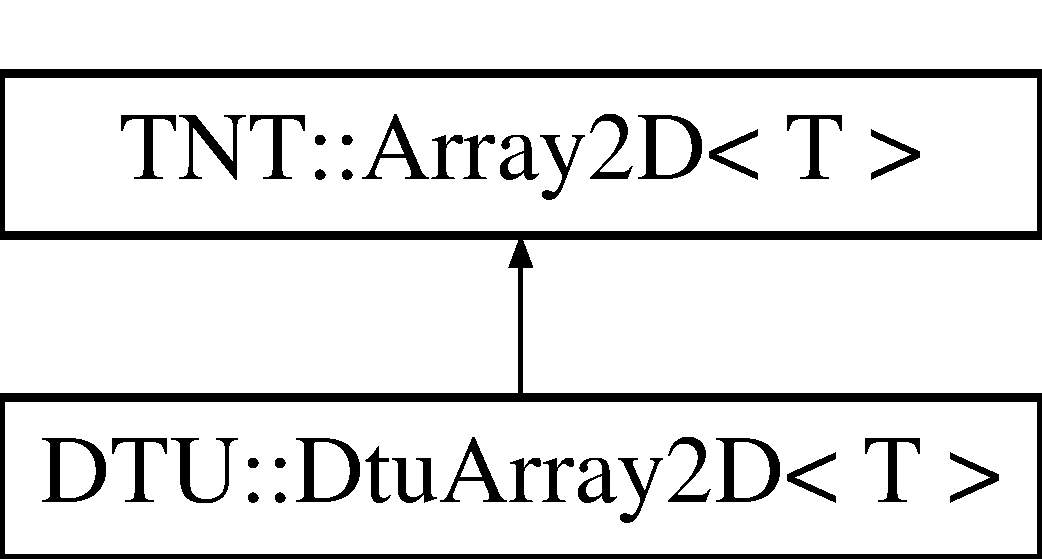
\includegraphics[height=2.000000cm]{classDTU_1_1DtuArray2D}
\end{center}
\end{figure}
\subsection*{Public Types}
\begin{DoxyCompactItemize}
\item 
typedef T \hyperlink{classDTU_1_1DtuArray2D_afd205bf3e12c0c1a57d0a451fd45446d}{value\-\_\-type}
\end{DoxyCompactItemize}
\subsection*{Public Member Functions}
\begin{DoxyCompactItemize}
\item 
\hyperlink{classDTU_1_1DtuArray2D_a6e06c78ecfbd2efdbe3c3e13df18c4c7}{Dtu\-Array2\-D} ()
\item 
\hyperlink{classDTU_1_1DtuArray2D_a1095f0d0a7f8ca187c15b4ef5488f68d}{Dtu\-Array2\-D} (int m, int n)
\item 
\hyperlink{classDTU_1_1DtuArray2D_af581f4e57787b3d46be392ce28f75fe9}{Dtu\-Array2\-D} (int m, int n, T $\ast$a)
\item 
\hyperlink{classDTU_1_1DtuArray2D_a1190f5752ba914133a2a77449ce56a05}{Dtu\-Array2\-D} (int m, int n, const T \&a)
\item 
\hyperlink{classDTU_1_1DtuArray2D_a88e0a39a0a5e84e14eee359ebb2bd3e1}{Dtu\-Array2\-D} (const \hyperlink{classTNT_1_1Array2D}{T\-N\-T\-::\-Array2\-D}$<$ T $>$ \&A)
\item 
\hyperlink{classDTU_1_1DtuArray2D}{Dtu\-Array2\-D} \& \hyperlink{classDTU_1_1DtuArray2D_a3ce392195f883257dc8133f7fab9564d}{operator=} (const T \&a)
\item 
int \hyperlink{classDTU_1_1DtuArray2D_a1c57e7cdb472b95640e16f69b664d797}{add} (const \hyperlink{classDTU_1_1DtuArray2D}{Dtu\-Array2\-D}$<$ T $>$ $\ast$B, \hyperlink{classDTU_1_1DtuArray2D}{Dtu\-Array2\-D}$<$ T $>$ $\ast$out)
\item 
int \hyperlink{classDTU_1_1DtuArray2D_aef64358747786ad8a0223161086cc7d0}{subtract} (const \hyperlink{classDTU_1_1DtuArray2D}{Dtu\-Array2\-D}$<$ T $>$ $\ast$B, \hyperlink{classDTU_1_1DtuArray2D}{Dtu\-Array2\-D}$<$ T $>$ $\ast$out)
\item 
void \hyperlink{classDTU_1_1DtuArray2D_aa395f408b57f194d773d309b5bcb3107}{multiply} (double scalar, \hyperlink{classDTU_1_1DtuArray2D}{Dtu\-Array2\-D}$<$ T $>$ $\ast$out)
\item 
int \hyperlink{classDTU_1_1DtuArray2D_af5b3ec0622fd426688ea0ab77b26db51}{multiply} (const \hyperlink{classDTU_1_1DtuArray2D}{Dtu\-Array2\-D}$<$ T $>$ $\ast$B, \hyperlink{classDTU_1_1DtuArray2D}{Dtu\-Array2\-D}$<$ T $>$ $\ast$out)
\item 
int \hyperlink{classDTU_1_1DtuArray2D_abfd1831b2f3ff56bb30ebae5a5b59b63}{multiply\-R} (const \hyperlink{classDTU_1_1DtuArray2D}{Dtu\-Array2\-D}$<$ T $>$ \&B, \hyperlink{classDTU_1_1DtuArray2D}{Dtu\-Array2\-D}$<$ T $>$ \&out)
\item 
int \hyperlink{classDTU_1_1DtuArray2D_a1d0e65eb4b55f8f7821adf7888fc6b5a}{multiply} (const \hyperlink{classDTU_1_1DtuArray2D}{Dtu\-Array2\-D}$<$ T $>$ $\ast$B, double scalar, \hyperlink{classDTU_1_1DtuArray2D}{Dtu\-Array2\-D}$<$ T $>$ $\ast$out)
\item 
void \hyperlink{classDTU_1_1DtuArray2D_af581f022e7453af3da50685391f71f35}{transpose} (\hyperlink{classDTU_1_1DtuArray2D}{Dtu\-Array2\-D}$<$ T $>$ $\ast$A)
\item 
void \hyperlink{classDTU_1_1DtuArray2D_a076b2f5fced5f94eff5f21c51ad80961}{transpose} (\hyperlink{classDTU_1_1DtuArray2D}{Dtu\-Array2\-D}$<$ T $>$ \&A)
\item 
int \hyperlink{classDTU_1_1DtuArray2D_a95044424cf0a7805be6bcddb6b2683f2}{transpose\-\_\-insitu} ()
\item 
int \hyperlink{classDTU_1_1DtuArray2D_a817f8d8127c60c21481e42531389376c}{get\-S\-V\-D} (\hyperlink{classJAMA_1_1SVD}{J\-A\-M\-A\-::\-S\-V\-D}$<$ T $>$ \&A)
\item 
void \hyperlink{classDTU_1_1DtuArray2D_ac84d734c8563a5abd76a043fc3c3a0e6}{pinv} (\hyperlink{classDTU_1_1DtuArray2D}{Dtu\-Array2\-D}$<$ T $>$ $\ast$A)
\item 
T \hyperlink{classDTU_1_1DtuArray2D_a8a8b977b5acee1e45c175b188685779b}{trace} ()
\item 
void \hyperlink{classDTU_1_1DtuArray2D_aecc0518069f41f2e12e88b35933e3573}{to\-Identity\-Matrix} ()
\item 
int \hyperlink{classDTU_1_1DtuArray2D_a68ddbc5c53f0e19a2fc2bae855e36077}{dim1} () const 
\item 
int \hyperlink{classDTU_1_1DtuArray2D_aefec13b0e62c9b7f56b6109f47ea757e}{dim2} () const 
\item 
\hyperlink{classTNT_1_1Array2D}{T\-N\-T\-::\-Array2\-D}$<$ T $>$ \hyperlink{classDTU_1_1DtuArray2D_a906c78d88bdb45a4f9d8805d3a0c6262}{to\-Tnt\-Array2\-D} ()
\item 
void \hyperlink{classDTU_1_1DtuArray2D_a3d918f63f7cb85cdc05739ac4c79807c}{print} ()
\end{DoxyCompactItemize}
\subsection*{Additional Inherited Members}


\subsection{Member Typedef Documentation}
\hypertarget{classDTU_1_1DtuArray2D_afd205bf3e12c0c1a57d0a451fd45446d}{\index{D\-T\-U\-::\-Dtu\-Array2\-D@{D\-T\-U\-::\-Dtu\-Array2\-D}!value\-\_\-type@{value\-\_\-type}}
\index{value\-\_\-type@{value\-\_\-type}!DTU::DtuArray2D@{D\-T\-U\-::\-Dtu\-Array2\-D}}
\subsubsection[{value\-\_\-type}]{\setlength{\rightskip}{0pt plus 5cm}template$<$class T$>$ typedef T {\bf D\-T\-U\-::\-Dtu\-Array2\-D}$<$ T $>$\-::{\bf value\-\_\-type}}}\label{classDTU_1_1DtuArray2D_afd205bf3e12c0c1a57d0a451fd45446d}


\subsection{Constructor \& Destructor Documentation}
\hypertarget{classDTU_1_1DtuArray2D_a6e06c78ecfbd2efdbe3c3e13df18c4c7}{\index{D\-T\-U\-::\-Dtu\-Array2\-D@{D\-T\-U\-::\-Dtu\-Array2\-D}!Dtu\-Array2\-D@{Dtu\-Array2\-D}}
\index{Dtu\-Array2\-D@{Dtu\-Array2\-D}!DTU::DtuArray2D@{D\-T\-U\-::\-Dtu\-Array2\-D}}
\subsubsection[{Dtu\-Array2\-D}]{\setlength{\rightskip}{0pt plus 5cm}template$<$class T$>$ {\bf D\-T\-U\-::\-Dtu\-Array2\-D}$<$ T $>$\-::{\bf Dtu\-Array2\-D} (
\begin{DoxyParamCaption}
{}
\end{DoxyParamCaption}
)\hspace{0.3cm}{\ttfamily [inline]}}}\label{classDTU_1_1DtuArray2D_a6e06c78ecfbd2efdbe3c3e13df18c4c7}
\hypertarget{classDTU_1_1DtuArray2D_a1095f0d0a7f8ca187c15b4ef5488f68d}{\index{D\-T\-U\-::\-Dtu\-Array2\-D@{D\-T\-U\-::\-Dtu\-Array2\-D}!Dtu\-Array2\-D@{Dtu\-Array2\-D}}
\index{Dtu\-Array2\-D@{Dtu\-Array2\-D}!DTU::DtuArray2D@{D\-T\-U\-::\-Dtu\-Array2\-D}}
\subsubsection[{Dtu\-Array2\-D}]{\setlength{\rightskip}{0pt plus 5cm}template$<$class T$>$ {\bf D\-T\-U\-::\-Dtu\-Array2\-D}$<$ T $>$\-::{\bf Dtu\-Array2\-D} (
\begin{DoxyParamCaption}
\item[{int}]{m, }
\item[{int}]{n}
\end{DoxyParamCaption}
)\hspace{0.3cm}{\ttfamily [inline]}}}\label{classDTU_1_1DtuArray2D_a1095f0d0a7f8ca187c15b4ef5488f68d}
\hypertarget{classDTU_1_1DtuArray2D_af581f4e57787b3d46be392ce28f75fe9}{\index{D\-T\-U\-::\-Dtu\-Array2\-D@{D\-T\-U\-::\-Dtu\-Array2\-D}!Dtu\-Array2\-D@{Dtu\-Array2\-D}}
\index{Dtu\-Array2\-D@{Dtu\-Array2\-D}!DTU::DtuArray2D@{D\-T\-U\-::\-Dtu\-Array2\-D}}
\subsubsection[{Dtu\-Array2\-D}]{\setlength{\rightskip}{0pt plus 5cm}template$<$class T$>$ {\bf D\-T\-U\-::\-Dtu\-Array2\-D}$<$ T $>$\-::{\bf Dtu\-Array2\-D} (
\begin{DoxyParamCaption}
\item[{int}]{m, }
\item[{int}]{n, }
\item[{T $\ast$}]{a}
\end{DoxyParamCaption}
)\hspace{0.3cm}{\ttfamily [inline]}}}\label{classDTU_1_1DtuArray2D_af581f4e57787b3d46be392ce28f75fe9}
\hypertarget{classDTU_1_1DtuArray2D_a1190f5752ba914133a2a77449ce56a05}{\index{D\-T\-U\-::\-Dtu\-Array2\-D@{D\-T\-U\-::\-Dtu\-Array2\-D}!Dtu\-Array2\-D@{Dtu\-Array2\-D}}
\index{Dtu\-Array2\-D@{Dtu\-Array2\-D}!DTU::DtuArray2D@{D\-T\-U\-::\-Dtu\-Array2\-D}}
\subsubsection[{Dtu\-Array2\-D}]{\setlength{\rightskip}{0pt plus 5cm}template$<$class T$>$ {\bf D\-T\-U\-::\-Dtu\-Array2\-D}$<$ T $>$\-::{\bf Dtu\-Array2\-D} (
\begin{DoxyParamCaption}
\item[{int}]{m, }
\item[{int}]{n, }
\item[{const T \&}]{a}
\end{DoxyParamCaption}
)\hspace{0.3cm}{\ttfamily [inline]}}}\label{classDTU_1_1DtuArray2D_a1190f5752ba914133a2a77449ce56a05}
\hypertarget{classDTU_1_1DtuArray2D_a88e0a39a0a5e84e14eee359ebb2bd3e1}{\index{D\-T\-U\-::\-Dtu\-Array2\-D@{D\-T\-U\-::\-Dtu\-Array2\-D}!Dtu\-Array2\-D@{Dtu\-Array2\-D}}
\index{Dtu\-Array2\-D@{Dtu\-Array2\-D}!DTU::DtuArray2D@{D\-T\-U\-::\-Dtu\-Array2\-D}}
\subsubsection[{Dtu\-Array2\-D}]{\setlength{\rightskip}{0pt plus 5cm}template$<$class T$>$ {\bf D\-T\-U\-::\-Dtu\-Array2\-D}$<$ T $>$\-::{\bf Dtu\-Array2\-D} (
\begin{DoxyParamCaption}
\item[{const {\bf T\-N\-T\-::\-Array2\-D}$<$ T $>$ \&}]{A}
\end{DoxyParamCaption}
)\hspace{0.3cm}{\ttfamily [inline]}}}\label{classDTU_1_1DtuArray2D_a88e0a39a0a5e84e14eee359ebb2bd3e1}


\subsection{Member Function Documentation}
\hypertarget{classDTU_1_1DtuArray2D_a1c57e7cdb472b95640e16f69b664d797}{\index{D\-T\-U\-::\-Dtu\-Array2\-D@{D\-T\-U\-::\-Dtu\-Array2\-D}!add@{add}}
\index{add@{add}!DTU::DtuArray2D@{D\-T\-U\-::\-Dtu\-Array2\-D}}
\subsubsection[{add}]{\setlength{\rightskip}{0pt plus 5cm}template$<$class T$>$ int {\bf D\-T\-U\-::\-Dtu\-Array2\-D}$<$ T $>$\-::add (
\begin{DoxyParamCaption}
\item[{const {\bf Dtu\-Array2\-D}$<$ T $>$ $\ast$}]{B, }
\item[{{\bf Dtu\-Array2\-D}$<$ T $>$ $\ast$}]{out}
\end{DoxyParamCaption}
)}}\label{classDTU_1_1DtuArray2D_a1c57e7cdb472b95640e16f69b664d797}
basic maths \hypertarget{classDTU_1_1DtuArray2D_a68ddbc5c53f0e19a2fc2bae855e36077}{\index{D\-T\-U\-::\-Dtu\-Array2\-D@{D\-T\-U\-::\-Dtu\-Array2\-D}!dim1@{dim1}}
\index{dim1@{dim1}!DTU::DtuArray2D@{D\-T\-U\-::\-Dtu\-Array2\-D}}
\subsubsection[{dim1}]{\setlength{\rightskip}{0pt plus 5cm}template$<$class T$>$ int {\bf D\-T\-U\-::\-Dtu\-Array2\-D}$<$ T $>$\-::dim1 (
\begin{DoxyParamCaption}
{}
\end{DoxyParamCaption}
) const\hspace{0.3cm}{\ttfamily [inline]}}}\label{classDTU_1_1DtuArray2D_a68ddbc5c53f0e19a2fc2bae855e36077}
\hypertarget{classDTU_1_1DtuArray2D_aefec13b0e62c9b7f56b6109f47ea757e}{\index{D\-T\-U\-::\-Dtu\-Array2\-D@{D\-T\-U\-::\-Dtu\-Array2\-D}!dim2@{dim2}}
\index{dim2@{dim2}!DTU::DtuArray2D@{D\-T\-U\-::\-Dtu\-Array2\-D}}
\subsubsection[{dim2}]{\setlength{\rightskip}{0pt plus 5cm}template$<$class T$>$ int {\bf D\-T\-U\-::\-Dtu\-Array2\-D}$<$ T $>$\-::dim2 (
\begin{DoxyParamCaption}
{}
\end{DoxyParamCaption}
) const\hspace{0.3cm}{\ttfamily [inline]}}}\label{classDTU_1_1DtuArray2D_aefec13b0e62c9b7f56b6109f47ea757e}
\hypertarget{classDTU_1_1DtuArray2D_a817f8d8127c60c21481e42531389376c}{\index{D\-T\-U\-::\-Dtu\-Array2\-D@{D\-T\-U\-::\-Dtu\-Array2\-D}!get\-S\-V\-D@{get\-S\-V\-D}}
\index{get\-S\-V\-D@{get\-S\-V\-D}!DTU::DtuArray2D@{D\-T\-U\-::\-Dtu\-Array2\-D}}
\subsubsection[{get\-S\-V\-D}]{\setlength{\rightskip}{0pt plus 5cm}template$<$class T$>$ int {\bf D\-T\-U\-::\-Dtu\-Array2\-D}$<$ T $>$\-::get\-S\-V\-D (
\begin{DoxyParamCaption}
\item[{{\bf J\-A\-M\-A\-::\-S\-V\-D}$<$ T $>$ \&}]{A}
\end{DoxyParamCaption}
)}}\label{classDTU_1_1DtuArray2D_a817f8d8127c60c21481e42531389376c}
\hypertarget{classDTU_1_1DtuArray2D_aa395f408b57f194d773d309b5bcb3107}{\index{D\-T\-U\-::\-Dtu\-Array2\-D@{D\-T\-U\-::\-Dtu\-Array2\-D}!multiply@{multiply}}
\index{multiply@{multiply}!DTU::DtuArray2D@{D\-T\-U\-::\-Dtu\-Array2\-D}}
\subsubsection[{multiply}]{\setlength{\rightskip}{0pt plus 5cm}template$<$class T$>$ void {\bf D\-T\-U\-::\-Dtu\-Array2\-D}$<$ T $>$\-::multiply (
\begin{DoxyParamCaption}
\item[{double}]{scalar, }
\item[{{\bf Dtu\-Array2\-D}$<$ T $>$ $\ast$}]{out}
\end{DoxyParamCaption}
)}}\label{classDTU_1_1DtuArray2D_aa395f408b57f194d773d309b5bcb3107}
\hypertarget{classDTU_1_1DtuArray2D_af5b3ec0622fd426688ea0ab77b26db51}{\index{D\-T\-U\-::\-Dtu\-Array2\-D@{D\-T\-U\-::\-Dtu\-Array2\-D}!multiply@{multiply}}
\index{multiply@{multiply}!DTU::DtuArray2D@{D\-T\-U\-::\-Dtu\-Array2\-D}}
\subsubsection[{multiply}]{\setlength{\rightskip}{0pt plus 5cm}template$<$class T$>$ int {\bf D\-T\-U\-::\-Dtu\-Array2\-D}$<$ T $>$\-::multiply (
\begin{DoxyParamCaption}
\item[{const {\bf Dtu\-Array2\-D}$<$ T $>$ $\ast$}]{B, }
\item[{{\bf Dtu\-Array2\-D}$<$ T $>$ $\ast$}]{out}
\end{DoxyParamCaption}
)}}\label{classDTU_1_1DtuArray2D_af5b3ec0622fd426688ea0ab77b26db51}
\hypertarget{classDTU_1_1DtuArray2D_a1d0e65eb4b55f8f7821adf7888fc6b5a}{\index{D\-T\-U\-::\-Dtu\-Array2\-D@{D\-T\-U\-::\-Dtu\-Array2\-D}!multiply@{multiply}}
\index{multiply@{multiply}!DTU::DtuArray2D@{D\-T\-U\-::\-Dtu\-Array2\-D}}
\subsubsection[{multiply}]{\setlength{\rightskip}{0pt plus 5cm}template$<$class T$>$ int {\bf D\-T\-U\-::\-Dtu\-Array2\-D}$<$ T $>$\-::multiply (
\begin{DoxyParamCaption}
\item[{const {\bf Dtu\-Array2\-D}$<$ T $>$ $\ast$}]{B, }
\item[{double}]{constant, }
\item[{{\bf Dtu\-Array2\-D}$<$ T $>$ $\ast$}]{out}
\end{DoxyParamCaption}
)}}\label{classDTU_1_1DtuArray2D_a1d0e65eb4b55f8f7821adf7888fc6b5a}
see int Dtu\-Array2\-D$<$\-T$>$\-::multiply(const Array2\-D$<$\-T$>$ \&\-B, Dtu\-Array2\-D$<$\-T$>$ \&out) for alternative implementations of multiplication \hypertarget{classDTU_1_1DtuArray2D_abfd1831b2f3ff56bb30ebae5a5b59b63}{\index{D\-T\-U\-::\-Dtu\-Array2\-D@{D\-T\-U\-::\-Dtu\-Array2\-D}!multiply\-R@{multiply\-R}}
\index{multiply\-R@{multiply\-R}!DTU::DtuArray2D@{D\-T\-U\-::\-Dtu\-Array2\-D}}
\subsubsection[{multiply\-R}]{\setlength{\rightskip}{0pt plus 5cm}template$<$class T$>$ int {\bf D\-T\-U\-::\-Dtu\-Array2\-D}$<$ T $>$\-::multiply\-R (
\begin{DoxyParamCaption}
\item[{const {\bf Dtu\-Array2\-D}$<$ T $>$ \&}]{B, }
\item[{{\bf Dtu\-Array2\-D}$<$ T $>$ \&}]{out}
\end{DoxyParamCaption}
)}}\label{classDTU_1_1DtuArray2D_abfd1831b2f3ff56bb30ebae5a5b59b63}
\hypertarget{classDTU_1_1DtuArray2D_a3ce392195f883257dc8133f7fab9564d}{\index{D\-T\-U\-::\-Dtu\-Array2\-D@{D\-T\-U\-::\-Dtu\-Array2\-D}!operator=@{operator=}}
\index{operator=@{operator=}!DTU::DtuArray2D@{D\-T\-U\-::\-Dtu\-Array2\-D}}
\subsubsection[{operator=}]{\setlength{\rightskip}{0pt plus 5cm}template$<$class T$>$ {\bf Dtu\-Array2\-D}$<$ T $>$ \& {\bf D\-T\-U\-::\-Dtu\-Array2\-D}$<$ T $>$\-::operator= (
\begin{DoxyParamCaption}
\item[{const T \&}]{a}
\end{DoxyParamCaption}
)\hspace{0.3cm}{\ttfamily [inline]}}}\label{classDTU_1_1DtuArray2D_a3ce392195f883257dc8133f7fab9564d}
\hypertarget{classDTU_1_1DtuArray2D_ac84d734c8563a5abd76a043fc3c3a0e6}{\index{D\-T\-U\-::\-Dtu\-Array2\-D@{D\-T\-U\-::\-Dtu\-Array2\-D}!pinv@{pinv}}
\index{pinv@{pinv}!DTU::DtuArray2D@{D\-T\-U\-::\-Dtu\-Array2\-D}}
\subsubsection[{pinv}]{\setlength{\rightskip}{0pt plus 5cm}template$<$class T$>$ void {\bf D\-T\-U\-::\-Dtu\-Array2\-D}$<$ T $>$\-::pinv (
\begin{DoxyParamCaption}
\item[{{\bf Dtu\-Array2\-D}$<$ T $>$ $\ast$}]{A}
\end{DoxyParamCaption}
)}}\label{classDTU_1_1DtuArray2D_ac84d734c8563a5abd76a043fc3c3a0e6}
\hypertarget{classDTU_1_1DtuArray2D_a3d918f63f7cb85cdc05739ac4c79807c}{\index{D\-T\-U\-::\-Dtu\-Array2\-D@{D\-T\-U\-::\-Dtu\-Array2\-D}!print@{print}}
\index{print@{print}!DTU::DtuArray2D@{D\-T\-U\-::\-Dtu\-Array2\-D}}
\subsubsection[{print}]{\setlength{\rightskip}{0pt plus 5cm}template$<$class T $>$ void {\bf D\-T\-U\-::\-Dtu\-Array2\-D}$<$ T $>$\-::print (
\begin{DoxyParamCaption}
{}
\end{DoxyParamCaption}
)\hspace{0.3cm}{\ttfamily [inline]}}}\label{classDTU_1_1DtuArray2D_a3d918f63f7cb85cdc05739ac4c79807c}
\hypertarget{classDTU_1_1DtuArray2D_aef64358747786ad8a0223161086cc7d0}{\index{D\-T\-U\-::\-Dtu\-Array2\-D@{D\-T\-U\-::\-Dtu\-Array2\-D}!subtract@{subtract}}
\index{subtract@{subtract}!DTU::DtuArray2D@{D\-T\-U\-::\-Dtu\-Array2\-D}}
\subsubsection[{subtract}]{\setlength{\rightskip}{0pt plus 5cm}template$<$class T$>$ int {\bf D\-T\-U\-::\-Dtu\-Array2\-D}$<$ T $>$\-::subtract (
\begin{DoxyParamCaption}
\item[{const {\bf Dtu\-Array2\-D}$<$ T $>$ $\ast$}]{B, }
\item[{{\bf Dtu\-Array2\-D}$<$ T $>$ $\ast$}]{out}
\end{DoxyParamCaption}
)}}\label{classDTU_1_1DtuArray2D_aef64358747786ad8a0223161086cc7d0}
\hypertarget{classDTU_1_1DtuArray2D_aecc0518069f41f2e12e88b35933e3573}{\index{D\-T\-U\-::\-Dtu\-Array2\-D@{D\-T\-U\-::\-Dtu\-Array2\-D}!to\-Identity\-Matrix@{to\-Identity\-Matrix}}
\index{to\-Identity\-Matrix@{to\-Identity\-Matrix}!DTU::DtuArray2D@{D\-T\-U\-::\-Dtu\-Array2\-D}}
\subsubsection[{to\-Identity\-Matrix}]{\setlength{\rightskip}{0pt plus 5cm}template$<$class T $>$ void {\bf D\-T\-U\-::\-Dtu\-Array2\-D}$<$ T $>$\-::to\-Identity\-Matrix (
\begin{DoxyParamCaption}
{}
\end{DoxyParamCaption}
)\hspace{0.3cm}{\ttfamily [inline]}}}\label{classDTU_1_1DtuArray2D_aecc0518069f41f2e12e88b35933e3573}
\hypertarget{classDTU_1_1DtuArray2D_a906c78d88bdb45a4f9d8805d3a0c6262}{\index{D\-T\-U\-::\-Dtu\-Array2\-D@{D\-T\-U\-::\-Dtu\-Array2\-D}!to\-Tnt\-Array2\-D@{to\-Tnt\-Array2\-D}}
\index{to\-Tnt\-Array2\-D@{to\-Tnt\-Array2\-D}!DTU::DtuArray2D@{D\-T\-U\-::\-Dtu\-Array2\-D}}
\subsubsection[{to\-Tnt\-Array2\-D}]{\setlength{\rightskip}{0pt plus 5cm}template$<$class T $>$ {\bf T\-N\-T\-::\-Array2\-D}$<$ T $>$ {\bf D\-T\-U\-::\-Dtu\-Array2\-D}$<$ T $>$\-::to\-Tnt\-Array2\-D (
\begin{DoxyParamCaption}
{}
\end{DoxyParamCaption}
)\hspace{0.3cm}{\ttfamily [inline]}}}\label{classDTU_1_1DtuArray2D_a906c78d88bdb45a4f9d8805d3a0c6262}
\hypertarget{classDTU_1_1DtuArray2D_a8a8b977b5acee1e45c175b188685779b}{\index{D\-T\-U\-::\-Dtu\-Array2\-D@{D\-T\-U\-::\-Dtu\-Array2\-D}!trace@{trace}}
\index{trace@{trace}!DTU::DtuArray2D@{D\-T\-U\-::\-Dtu\-Array2\-D}}
\subsubsection[{trace}]{\setlength{\rightskip}{0pt plus 5cm}template$<$class T $>$ T {\bf D\-T\-U\-::\-Dtu\-Array2\-D}$<$ T $>$\-::trace (
\begin{DoxyParamCaption}
{}
\end{DoxyParamCaption}
)\hspace{0.3cm}{\ttfamily [inline]}}}\label{classDTU_1_1DtuArray2D_a8a8b977b5acee1e45c175b188685779b}
\hypertarget{classDTU_1_1DtuArray2D_af581f022e7453af3da50685391f71f35}{\index{D\-T\-U\-::\-Dtu\-Array2\-D@{D\-T\-U\-::\-Dtu\-Array2\-D}!transpose@{transpose}}
\index{transpose@{transpose}!DTU::DtuArray2D@{D\-T\-U\-::\-Dtu\-Array2\-D}}
\subsubsection[{transpose}]{\setlength{\rightskip}{0pt plus 5cm}template$<$class T$>$ void {\bf D\-T\-U\-::\-Dtu\-Array2\-D}$<$ T $>$\-::transpose (
\begin{DoxyParamCaption}
\item[{{\bf Dtu\-Array2\-D}$<$ T $>$ $\ast$}]{A}
\end{DoxyParamCaption}
)}}\label{classDTU_1_1DtuArray2D_af581f022e7453af3da50685391f71f35}
array operations \hypertarget{classDTU_1_1DtuArray2D_a076b2f5fced5f94eff5f21c51ad80961}{\index{D\-T\-U\-::\-Dtu\-Array2\-D@{D\-T\-U\-::\-Dtu\-Array2\-D}!transpose@{transpose}}
\index{transpose@{transpose}!DTU::DtuArray2D@{D\-T\-U\-::\-Dtu\-Array2\-D}}
\subsubsection[{transpose}]{\setlength{\rightskip}{0pt plus 5cm}template$<$class T$>$ void {\bf D\-T\-U\-::\-Dtu\-Array2\-D}$<$ T $>$\-::transpose (
\begin{DoxyParamCaption}
\item[{{\bf Dtu\-Array2\-D}$<$ T $>$ \&}]{A}
\end{DoxyParamCaption}
)}}\label{classDTU_1_1DtuArray2D_a076b2f5fced5f94eff5f21c51ad80961}
\hypertarget{classDTU_1_1DtuArray2D_a95044424cf0a7805be6bcddb6b2683f2}{\index{D\-T\-U\-::\-Dtu\-Array2\-D@{D\-T\-U\-::\-Dtu\-Array2\-D}!transpose\-\_\-insitu@{transpose\-\_\-insitu}}
\index{transpose\-\_\-insitu@{transpose\-\_\-insitu}!DTU::DtuArray2D@{D\-T\-U\-::\-Dtu\-Array2\-D}}
\subsubsection[{transpose\-\_\-insitu}]{\setlength{\rightskip}{0pt plus 5cm}template$<$class T $>$ int {\bf D\-T\-U\-::\-Dtu\-Array2\-D}$<$ T $>$\-::transpose\-\_\-insitu (
\begin{DoxyParamCaption}
{}
\end{DoxyParamCaption}
)}}\label{classDTU_1_1DtuArray2D_a95044424cf0a7805be6bcddb6b2683f2}


The documentation for this class was generated from the following file\-:\begin{DoxyCompactItemize}
\item 
/media/philipjhj/\-Data/\-One\-Drive/\-Studie/\-Studenterprogrammør/\-S\-B\-S3/smartphonebrainscanner2-\/core/src/\hyperlink{dtu__array__2d_8h}{dtu\-\_\-array\-\_\-2d.\-h}\end{DoxyCompactItemize}

\hypertarget{classJAMA_1_1Eigenvalue}{\section{J\-A\-M\-A\-:\-:Eigenvalue$<$ Real $>$ Class Template Reference}
\label{classJAMA_1_1Eigenvalue}\index{J\-A\-M\-A\-::\-Eigenvalue$<$ Real $>$@{J\-A\-M\-A\-::\-Eigenvalue$<$ Real $>$}}
}


{\ttfamily \#include $<$jama\-\_\-eig.\-h$>$}

\subsection*{Public Member Functions}
\begin{DoxyCompactItemize}
\item 
\hyperlink{classJAMA_1_1Eigenvalue_a28bf3e2df18bcd3d3f3b0979630953b3}{Eigenvalue} (const \hyperlink{classTNT_1_1Array2D}{T\-N\-T\-::\-Array2\-D}$<$ Real $>$ \&A)
\item 
void \hyperlink{classJAMA_1_1Eigenvalue_ad01bfc213b887979f8f702acdd0a76c2}{get\-V} (\hyperlink{classTNT_1_1Array2D}{T\-N\-T\-::\-Array2\-D}$<$ Real $>$ \&V\-\_\-)
\item 
void \hyperlink{classJAMA_1_1Eigenvalue_aae525e0f58b9ea03f183a4a75b46af50}{get\-Real\-Eigenvalues} (\hyperlink{classTNT_1_1Array1D}{T\-N\-T\-::\-Array1\-D}$<$ Real $>$ \&d\-\_\-)
\item 
void \hyperlink{classJAMA_1_1Eigenvalue_ad72ed4bd3a07325097a1ef4e36a0480f}{get\-Imag\-Eigenvalues} (\hyperlink{classTNT_1_1Array1D}{T\-N\-T\-::\-Array1\-D}$<$ Real $>$ \&e\-\_\-)
\item 
void \hyperlink{classJAMA_1_1Eigenvalue_aee57a1213656385928a3fb2c6a21e4b2}{get\-D} (\hyperlink{classTNT_1_1Array2D}{T\-N\-T\-::\-Array2\-D}$<$ Real $>$ \&D)
\end{DoxyCompactItemize}


\subsection{Detailed Description}
\subsubsection*{template$<$class Real$>$class J\-A\-M\-A\-::\-Eigenvalue$<$ Real $>$}

Computes eigenvalues and eigenvectors of a real (non-\/complex) matrix. 

If A is symmetric, then A = V$\ast$\-D$\ast$\-V' where the eigenvalue matrix D is diagonal and the eigenvector matrix V is orthogonal. That is, the diagonal values of D are the eigenvalues, and V$\ast$\-V' = I, where I is the identity matrix. The columns of V represent the eigenvectors in the sense that A$\ast$\-V = V$\ast$\-D.

If A is not symmetric, then the eigenvalue matrix D is block diagonal with the real eigenvalues in 1-\/by-\/1 blocks and any complex eigenvalues, a + i$\ast$b, in 2-\/by-\/2 blocks, \mbox{[}a, b; -\/b, a\mbox{]}. That is, if the complex eigenvalues look like 
\begin{DoxyPre}\end{DoxyPre}



\begin{DoxyPre}          u + iv     .        .          .      .    .
            .      u - iv     .          .      .    .
            .        .      a + ib       .      .    .
            .        .        .        a - ib   .    .
            .        .        .          .      x    .
            .        .        .          .      .    y
\end{DoxyPre}
 then D looks like 
\begin{DoxyPre}\end{DoxyPre}



\begin{DoxyPre}            u        v        .          .      .    .
           -v        u        .          .      .    . 
            .        .        a          b      .    .
            .        .       -b          a      .    .
            .        .        .          .      x    .
            .        .        .          .      .    y
\end{DoxyPre}
 This keeps V a real matrix in both symmetric and non-\/symmetric cases, and A$\ast$\-V = V$\ast$\-D.

\begin{DoxyVerb}<p>
The matrix V may be badly
conditioned, or even singular, so the validity of the equation
A = V*D*inverse(V) depends upon the condition number of V.
\end{DoxyVerb}


(Adapted from \hyperlink{namespaceJAMA}{J\-A\-M\-A}, a Java Matrix Library, developed by jointly by the Mathworks and N\-I\-S\-T; see \href{http://math.nist.gov/javanumerics/jama}{\tt http\-://math.\-nist.\-gov/javanumerics/jama}). 

\subsection{Constructor \& Destructor Documentation}
\hypertarget{classJAMA_1_1Eigenvalue_a28bf3e2df18bcd3d3f3b0979630953b3}{\index{J\-A\-M\-A\-::\-Eigenvalue@{J\-A\-M\-A\-::\-Eigenvalue}!Eigenvalue@{Eigenvalue}}
\index{Eigenvalue@{Eigenvalue}!JAMA::Eigenvalue@{J\-A\-M\-A\-::\-Eigenvalue}}
\subsubsection[{Eigenvalue}]{\setlength{\rightskip}{0pt plus 5cm}template$<$class Real $>$ {\bf J\-A\-M\-A\-::\-Eigenvalue}$<$ Real $>$\-::{\bf Eigenvalue} (
\begin{DoxyParamCaption}
\item[{const {\bf T\-N\-T\-::\-Array2\-D}$<$ Real $>$ \&}]{A}
\end{DoxyParamCaption}
)\hspace{0.3cm}{\ttfamily [inline]}}}\label{classJAMA_1_1Eigenvalue_a28bf3e2df18bcd3d3f3b0979630953b3}
Check for symmetry, then construct the eigenvalue decomposition 
\begin{DoxyParams}{Parameters}
{\em A} & Square real (non-\/complex) matrix \\
\hline
\end{DoxyParams}


\subsection{Member Function Documentation}
\hypertarget{classJAMA_1_1Eigenvalue_aee57a1213656385928a3fb2c6a21e4b2}{\index{J\-A\-M\-A\-::\-Eigenvalue@{J\-A\-M\-A\-::\-Eigenvalue}!get\-D@{get\-D}}
\index{get\-D@{get\-D}!JAMA::Eigenvalue@{J\-A\-M\-A\-::\-Eigenvalue}}
\subsubsection[{get\-D}]{\setlength{\rightskip}{0pt plus 5cm}template$<$class Real $>$ void {\bf J\-A\-M\-A\-::\-Eigenvalue}$<$ Real $>$\-::get\-D (
\begin{DoxyParamCaption}
\item[{{\bf T\-N\-T\-::\-Array2\-D}$<$ Real $>$ \&}]{D}
\end{DoxyParamCaption}
)\hspace{0.3cm}{\ttfamily [inline]}}}\label{classJAMA_1_1Eigenvalue_aee57a1213656385928a3fb2c6a21e4b2}
Computes the block diagonal eigenvalue matrix. If the original matrix A is not symmetric, then the eigenvalue matrix D is block diagonal with the real eigenvalues in 1-\/by-\/1 blocks and any complex eigenvalues, a + i$\ast$b, in 2-\/by-\/2 blocks, \mbox{[}a, b; -\/b, a\mbox{]}. That is, if the complex eigenvalues look like 
\begin{DoxyPre}\end{DoxyPre}



\begin{DoxyPre}          u + iv     .        .          .      .    .
            .      u - iv     .          .      .    .
            .        .      a + ib       .      .    .
            .        .        .        a - ib   .    .
            .        .        .          .      x    .
            .        .        .          .      .    y
\end{DoxyPre}
 then D looks like 
\begin{DoxyPre}\end{DoxyPre}



\begin{DoxyPre}            u        v        .          .      .    .
           -v        u        .          .      .    . 
            .        .        a          b      .    .
            .        .       -b          a      .    .
            .        .        .          .      x    .
            .        .        .          .      .    y
\end{DoxyPre}
 This keeps V a real matrix in both symmetric and non-\/symmetric cases, and A$\ast$\-V = V$\ast$\-D.


\begin{DoxyParams}{Parameters}
{\em D} & upon return, the matrix is filled with the block diagonal eigenvalue matrix. \\
\hline
\end{DoxyParams}
\hypertarget{classJAMA_1_1Eigenvalue_ad72ed4bd3a07325097a1ef4e36a0480f}{\index{J\-A\-M\-A\-::\-Eigenvalue@{J\-A\-M\-A\-::\-Eigenvalue}!get\-Imag\-Eigenvalues@{get\-Imag\-Eigenvalues}}
\index{get\-Imag\-Eigenvalues@{get\-Imag\-Eigenvalues}!JAMA::Eigenvalue@{J\-A\-M\-A\-::\-Eigenvalue}}
\subsubsection[{get\-Imag\-Eigenvalues}]{\setlength{\rightskip}{0pt plus 5cm}template$<$class Real $>$ void {\bf J\-A\-M\-A\-::\-Eigenvalue}$<$ Real $>$\-::get\-Imag\-Eigenvalues (
\begin{DoxyParamCaption}
\item[{{\bf T\-N\-T\-::\-Array1\-D}$<$ Real $>$ \&}]{e\-\_\-}
\end{DoxyParamCaption}
)\hspace{0.3cm}{\ttfamily [inline]}}}\label{classJAMA_1_1Eigenvalue_ad72ed4bd3a07325097a1ef4e36a0480f}
Return the imaginary parts of the eigenvalues in parameter e\-\_\-.

e\-\_\-\-: new matrix with imaginary parts of the eigenvalues. \hypertarget{classJAMA_1_1Eigenvalue_aae525e0f58b9ea03f183a4a75b46af50}{\index{J\-A\-M\-A\-::\-Eigenvalue@{J\-A\-M\-A\-::\-Eigenvalue}!get\-Real\-Eigenvalues@{get\-Real\-Eigenvalues}}
\index{get\-Real\-Eigenvalues@{get\-Real\-Eigenvalues}!JAMA::Eigenvalue@{J\-A\-M\-A\-::\-Eigenvalue}}
\subsubsection[{get\-Real\-Eigenvalues}]{\setlength{\rightskip}{0pt plus 5cm}template$<$class Real $>$ void {\bf J\-A\-M\-A\-::\-Eigenvalue}$<$ Real $>$\-::get\-Real\-Eigenvalues (
\begin{DoxyParamCaption}
\item[{{\bf T\-N\-T\-::\-Array1\-D}$<$ Real $>$ \&}]{d\-\_\-}
\end{DoxyParamCaption}
)\hspace{0.3cm}{\ttfamily [inline]}}}\label{classJAMA_1_1Eigenvalue_aae525e0f58b9ea03f183a4a75b46af50}
Return the real parts of the eigenvalues \begin{DoxyReturn}{Returns}
real(diag(\-D)) 
\end{DoxyReturn}
\hypertarget{classJAMA_1_1Eigenvalue_ad01bfc213b887979f8f702acdd0a76c2}{\index{J\-A\-M\-A\-::\-Eigenvalue@{J\-A\-M\-A\-::\-Eigenvalue}!get\-V@{get\-V}}
\index{get\-V@{get\-V}!JAMA::Eigenvalue@{J\-A\-M\-A\-::\-Eigenvalue}}
\subsubsection[{get\-V}]{\setlength{\rightskip}{0pt plus 5cm}template$<$class Real $>$ void {\bf J\-A\-M\-A\-::\-Eigenvalue}$<$ Real $>$\-::get\-V (
\begin{DoxyParamCaption}
\item[{{\bf T\-N\-T\-::\-Array2\-D}$<$ Real $>$ \&}]{V\-\_\-}
\end{DoxyParamCaption}
)\hspace{0.3cm}{\ttfamily [inline]}}}\label{classJAMA_1_1Eigenvalue_ad01bfc213b887979f8f702acdd0a76c2}
Return the eigenvector matrix \begin{DoxyReturn}{Returns}
V 
\end{DoxyReturn}


The documentation for this class was generated from the following file\-:\begin{DoxyCompactItemize}
\item 
/media/philipjhj/\-Data/\-One\-Drive/\-Studie/\-Studenterprogrammør/\-S\-B\-S3/smartphonebrainscanner2-\/core/src/jama125/\hyperlink{jama__eig_8h}{jama\-\_\-eig.\-h}\end{DoxyCompactItemize}

\hypertarget{classFFTReal}{\section{F\-F\-T\-Real Class Reference}
\label{classFFTReal}\index{F\-F\-T\-Real@{F\-F\-T\-Real}}
}


{\ttfamily \#include $<$F\-F\-T\-Real.\-h$>$}

\subsection*{Public Types}
\begin{DoxyCompactItemize}
\item 
typedef double \hyperlink{classFFTReal_ad9963e87c98cfa8a55544cd162e3fece}{flt\-\_\-t}
\end{DoxyCompactItemize}
\subsection*{Public Member Functions}
\begin{DoxyCompactItemize}
\item 
\hyperlink{classFFTReal_ac98f9b768dc122c212b6f6e4ce878e18}{F\-F\-T\-Real} (const long length)
\item 
\hyperlink{classFFTReal_a28ef7dceefba4ab73b3fecdb68a56334}{$\sim$\-F\-F\-T\-Real} ()
\item 
void \hyperlink{classFFTReal_aaef06fd9a9f9e070c5a64b8c4191c1b7}{do\-\_\-fft} (\hyperlink{classFFTReal_ad9963e87c98cfa8a55544cd162e3fece}{flt\-\_\-t} f\mbox{[}$\,$\mbox{]}, const \hyperlink{classFFTReal_ad9963e87c98cfa8a55544cd162e3fece}{flt\-\_\-t} x\mbox{[}$\,$\mbox{]}) const 
\item 
void \hyperlink{classFFTReal_a8a09a4f467150be6714a2895654e9c83}{do\-\_\-ifft} (const \hyperlink{classFFTReal_ad9963e87c98cfa8a55544cd162e3fece}{flt\-\_\-t} f\mbox{[}$\,$\mbox{]}, \hyperlink{classFFTReal_ad9963e87c98cfa8a55544cd162e3fece}{flt\-\_\-t} x\mbox{[}$\,$\mbox{]}) const 
\item 
void \hyperlink{classFFTReal_abf221c16cff2a4787765f4258c567a3a}{rescale} (\hyperlink{classFFTReal_ad9963e87c98cfa8a55544cd162e3fece}{flt\-\_\-t} x\mbox{[}$\,$\mbox{]}) const 
\end{DoxyCompactItemize}


\subsection{Member Typedef Documentation}
\hypertarget{classFFTReal_ad9963e87c98cfa8a55544cd162e3fece}{\index{F\-F\-T\-Real@{F\-F\-T\-Real}!flt\-\_\-t@{flt\-\_\-t}}
\index{flt\-\_\-t@{flt\-\_\-t}!FFTReal@{F\-F\-T\-Real}}
\subsubsection[{flt\-\_\-t}]{\setlength{\rightskip}{0pt plus 5cm}typedef double {\bf F\-F\-T\-Real\-::flt\-\_\-t}}}\label{classFFTReal_ad9963e87c98cfa8a55544cd162e3fece}


\subsection{Constructor \& Destructor Documentation}
\hypertarget{classFFTReal_ac98f9b768dc122c212b6f6e4ce878e18}{\index{F\-F\-T\-Real@{F\-F\-T\-Real}!F\-F\-T\-Real@{F\-F\-T\-Real}}
\index{F\-F\-T\-Real@{F\-F\-T\-Real}!FFTReal@{F\-F\-T\-Real}}
\subsubsection[{F\-F\-T\-Real}]{\setlength{\rightskip}{0pt plus 5cm}F\-F\-T\-Real\-::\-F\-F\-T\-Real (
\begin{DoxyParamCaption}
\item[{const long}]{length}
\end{DoxyParamCaption}
)\hspace{0.3cm}{\ttfamily [explicit]}}}\label{classFFTReal_ac98f9b768dc122c212b6f6e4ce878e18}
\hypertarget{classFFTReal_a28ef7dceefba4ab73b3fecdb68a56334}{\index{F\-F\-T\-Real@{F\-F\-T\-Real}!$\sim$\-F\-F\-T\-Real@{$\sim$\-F\-F\-T\-Real}}
\index{$\sim$\-F\-F\-T\-Real@{$\sim$\-F\-F\-T\-Real}!FFTReal@{F\-F\-T\-Real}}
\subsubsection[{$\sim$\-F\-F\-T\-Real}]{\setlength{\rightskip}{0pt plus 5cm}F\-F\-T\-Real\-::$\sim$\-F\-F\-T\-Real (
\begin{DoxyParamCaption}
\item[{void}]{}
\end{DoxyParamCaption}
)}}\label{classFFTReal_a28ef7dceefba4ab73b3fecdb68a56334}


\subsection{Member Function Documentation}
\hypertarget{classFFTReal_aaef06fd9a9f9e070c5a64b8c4191c1b7}{\index{F\-F\-T\-Real@{F\-F\-T\-Real}!do\-\_\-fft@{do\-\_\-fft}}
\index{do\-\_\-fft@{do\-\_\-fft}!FFTReal@{F\-F\-T\-Real}}
\subsubsection[{do\-\_\-fft}]{\setlength{\rightskip}{0pt plus 5cm}void F\-F\-T\-Real\-::do\-\_\-fft (
\begin{DoxyParamCaption}
\item[{{\bf flt\-\_\-t}}]{f\mbox{[}$\,$\mbox{]}, }
\item[{const {\bf flt\-\_\-t}}]{x\mbox{[}$\,$\mbox{]}}
\end{DoxyParamCaption}
) const}}\label{classFFTReal_aaef06fd9a9f9e070c5a64b8c4191c1b7}
\hypertarget{classFFTReal_a8a09a4f467150be6714a2895654e9c83}{\index{F\-F\-T\-Real@{F\-F\-T\-Real}!do\-\_\-ifft@{do\-\_\-ifft}}
\index{do\-\_\-ifft@{do\-\_\-ifft}!FFTReal@{F\-F\-T\-Real}}
\subsubsection[{do\-\_\-ifft}]{\setlength{\rightskip}{0pt plus 5cm}void F\-F\-T\-Real\-::do\-\_\-ifft (
\begin{DoxyParamCaption}
\item[{const {\bf flt\-\_\-t}}]{f\mbox{[}$\,$\mbox{]}, }
\item[{{\bf flt\-\_\-t}}]{x\mbox{[}$\,$\mbox{]}}
\end{DoxyParamCaption}
) const}}\label{classFFTReal_a8a09a4f467150be6714a2895654e9c83}
\hypertarget{classFFTReal_abf221c16cff2a4787765f4258c567a3a}{\index{F\-F\-T\-Real@{F\-F\-T\-Real}!rescale@{rescale}}
\index{rescale@{rescale}!FFTReal@{F\-F\-T\-Real}}
\subsubsection[{rescale}]{\setlength{\rightskip}{0pt plus 5cm}void F\-F\-T\-Real\-::rescale (
\begin{DoxyParamCaption}
\item[{{\bf flt\-\_\-t}}]{x\mbox{[}$\,$\mbox{]}}
\end{DoxyParamCaption}
) const}}\label{classFFTReal_abf221c16cff2a4787765f4258c567a3a}


The documentation for this class was generated from the following files\-:\begin{DoxyCompactItemize}
\item 
/media/philipjhj/\-Data/\-One\-Drive/\-Studie/\-Studenterprogrammør/\-S\-B\-S3/smartphonebrainscanner2-\/core/src/\hyperlink{FFTReal_8h}{F\-F\-T\-Real.\-h}\item 
/media/philipjhj/\-Data/\-One\-Drive/\-Studie/\-Studenterprogrammør/\-S\-B\-S3/smartphonebrainscanner2-\/core/src/\hyperlink{FFTReal_8cpp}{F\-F\-T\-Real.\-cpp}\end{DoxyCompactItemize}

\hypertarget{classTNT_1_1Fortran__Array1D}{\section{T\-N\-T\-:\-:Fortran\-\_\-\-Array1\-D$<$ T $>$ Class Template Reference}
\label{classTNT_1_1Fortran__Array1D}\index{T\-N\-T\-::\-Fortran\-\_\-\-Array1\-D$<$ T $>$@{T\-N\-T\-::\-Fortran\-\_\-\-Array1\-D$<$ T $>$}}
}


{\ttfamily \#include $<$tnt\-\_\-fortran\-\_\-array1d.\-h$>$}

\subsection*{Public Types}
\begin{DoxyCompactItemize}
\item 
typedef T \hyperlink{classTNT_1_1Fortran__Array1D_af213c3571890bd98e08eb5e93e100a1a}{value\-\_\-type}
\end{DoxyCompactItemize}
\subsection*{Public Member Functions}
\begin{DoxyCompactItemize}
\item 
\hyperlink{classTNT_1_1Fortran__Array1D_a8fade001c69d8de5c1dcbe578a334601}{Fortran\-\_\-\-Array1\-D} ()
\item 
\hyperlink{classTNT_1_1Fortran__Array1D_a44e447a75b9dfb163cb8262ac98e0f30}{Fortran\-\_\-\-Array1\-D} (int n)
\item 
\hyperlink{classTNT_1_1Fortran__Array1D_afce3a6a4930dbb0f4f4abcf6096108e0}{Fortran\-\_\-\-Array1\-D} (int n, const T \&a)
\item 
\hyperlink{classTNT_1_1Fortran__Array1D_ab15dda718952736b1c4ab0ae3821d301}{Fortran\-\_\-\-Array1\-D} (int n, T $\ast$a)
\item 
\hyperlink{classTNT_1_1Fortran__Array1D_a015f19a79b872d0b1097494656ea4c2d}{Fortran\-\_\-\-Array1\-D} (const \hyperlink{classTNT_1_1Fortran__Array1D}{Fortran\-\_\-\-Array1\-D} \&A)
\item 
\hyperlink{classTNT_1_1Fortran__Array1D}{Fortran\-\_\-\-Array1\-D} \& \hyperlink{classTNT_1_1Fortran__Array1D_ab6b262818e08afe5401fb8edbb12a00d}{operator=} (const T \&a)
\item 
\hyperlink{classTNT_1_1Fortran__Array1D}{Fortran\-\_\-\-Array1\-D} \& \hyperlink{classTNT_1_1Fortran__Array1D_a22a2465c8ca9540e588a3b3d3824f303}{operator=} (const \hyperlink{classTNT_1_1Fortran__Array1D}{Fortran\-\_\-\-Array1\-D} \&A)
\item 
\hyperlink{classTNT_1_1Fortran__Array1D}{Fortran\-\_\-\-Array1\-D} \& \hyperlink{classTNT_1_1Fortran__Array1D_a76788e78e69238822450782be69f851d}{ref} (const \hyperlink{classTNT_1_1Fortran__Array1D}{Fortran\-\_\-\-Array1\-D} \&A)
\item 
\hyperlink{classTNT_1_1Fortran__Array1D}{Fortran\-\_\-\-Array1\-D} \hyperlink{classTNT_1_1Fortran__Array1D_ad67336a534b20fa2a55cb60c9aaff2de}{copy} () const 
\item 
\hyperlink{classTNT_1_1Fortran__Array1D}{Fortran\-\_\-\-Array1\-D} \& \hyperlink{classTNT_1_1Fortran__Array1D_aef0affac0190dd180ac3ee56cccbcffb}{inject} (const \hyperlink{classTNT_1_1Fortran__Array1D}{Fortran\-\_\-\-Array1\-D} \&A)
\item 
T \& \hyperlink{classTNT_1_1Fortran__Array1D_a63779e6fa851280f20e41f5c36bf62c1}{operator()} (int i)
\item 
const T \& \hyperlink{classTNT_1_1Fortran__Array1D_ab7136972ebd6a6ccd43e9352054f9d1a}{operator()} (int i) const 
\item 
int \hyperlink{classTNT_1_1Fortran__Array1D_a38da25238999b4d5c23201cb5d748e46}{dim1} () const 
\item 
int \hyperlink{classTNT_1_1Fortran__Array1D_a60ce550d4a6dba1f8fbaa287a0cb7d0b}{dim} () const 
\item 
\hyperlink{classTNT_1_1Fortran__Array1D_aed735c33f3ff8f64c61c86ac4b163c1c}{$\sim$\-Fortran\-\_\-\-Array1\-D} ()
\item 
int \hyperlink{classTNT_1_1Fortran__Array1D_ad80b611a5af26ccd3ef62b0f1395e2f7}{ref\-\_\-count} () const 
\item 
\hyperlink{classTNT_1_1Fortran__Array1D}{Fortran\-\_\-\-Array1\-D}$<$ T $>$ \hyperlink{classTNT_1_1Fortran__Array1D_a6d4aad7e6e4ef4dfd1cf26e86a1d1311}{subarray} (int i0, int i1)
\end{DoxyCompactItemize}


\subsection{Member Typedef Documentation}
\hypertarget{classTNT_1_1Fortran__Array1D_af213c3571890bd98e08eb5e93e100a1a}{\index{T\-N\-T\-::\-Fortran\-\_\-\-Array1\-D@{T\-N\-T\-::\-Fortran\-\_\-\-Array1\-D}!value\-\_\-type@{value\-\_\-type}}
\index{value\-\_\-type@{value\-\_\-type}!TNT::Fortran_Array1D@{T\-N\-T\-::\-Fortran\-\_\-\-Array1\-D}}
\subsubsection[{value\-\_\-type}]{\setlength{\rightskip}{0pt plus 5cm}template$<$class T$>$ typedef T {\bf T\-N\-T\-::\-Fortran\-\_\-\-Array1\-D}$<$ T $>$\-::{\bf value\-\_\-type}}}\label{classTNT_1_1Fortran__Array1D_af213c3571890bd98e08eb5e93e100a1a}


\subsection{Constructor \& Destructor Documentation}
\hypertarget{classTNT_1_1Fortran__Array1D_a8fade001c69d8de5c1dcbe578a334601}{\index{T\-N\-T\-::\-Fortran\-\_\-\-Array1\-D@{T\-N\-T\-::\-Fortran\-\_\-\-Array1\-D}!Fortran\-\_\-\-Array1\-D@{Fortran\-\_\-\-Array1\-D}}
\index{Fortran\-\_\-\-Array1\-D@{Fortran\-\_\-\-Array1\-D}!TNT::Fortran_Array1D@{T\-N\-T\-::\-Fortran\-\_\-\-Array1\-D}}
\subsubsection[{Fortran\-\_\-\-Array1\-D}]{\setlength{\rightskip}{0pt plus 5cm}template$<$class T $>$ {\bf T\-N\-T\-::\-Fortran\-\_\-\-Array1\-D}$<$ T $>$\-::{\bf Fortran\-\_\-\-Array1\-D} (
\begin{DoxyParamCaption}
{}
\end{DoxyParamCaption}
)}}\label{classTNT_1_1Fortran__Array1D_a8fade001c69d8de5c1dcbe578a334601}
\hypertarget{classTNT_1_1Fortran__Array1D_a44e447a75b9dfb163cb8262ac98e0f30}{\index{T\-N\-T\-::\-Fortran\-\_\-\-Array1\-D@{T\-N\-T\-::\-Fortran\-\_\-\-Array1\-D}!Fortran\-\_\-\-Array1\-D@{Fortran\-\_\-\-Array1\-D}}
\index{Fortran\-\_\-\-Array1\-D@{Fortran\-\_\-\-Array1\-D}!TNT::Fortran_Array1D@{T\-N\-T\-::\-Fortran\-\_\-\-Array1\-D}}
\subsubsection[{Fortran\-\_\-\-Array1\-D}]{\setlength{\rightskip}{0pt plus 5cm}template$<$class T $>$ {\bf T\-N\-T\-::\-Fortran\-\_\-\-Array1\-D}$<$ T $>$\-::{\bf Fortran\-\_\-\-Array1\-D} (
\begin{DoxyParamCaption}
\item[{int}]{n}
\end{DoxyParamCaption}
)\hspace{0.3cm}{\ttfamily [explicit]}}}\label{classTNT_1_1Fortran__Array1D_a44e447a75b9dfb163cb8262ac98e0f30}
\hypertarget{classTNT_1_1Fortran__Array1D_afce3a6a4930dbb0f4f4abcf6096108e0}{\index{T\-N\-T\-::\-Fortran\-\_\-\-Array1\-D@{T\-N\-T\-::\-Fortran\-\_\-\-Array1\-D}!Fortran\-\_\-\-Array1\-D@{Fortran\-\_\-\-Array1\-D}}
\index{Fortran\-\_\-\-Array1\-D@{Fortran\-\_\-\-Array1\-D}!TNT::Fortran_Array1D@{T\-N\-T\-::\-Fortran\-\_\-\-Array1\-D}}
\subsubsection[{Fortran\-\_\-\-Array1\-D}]{\setlength{\rightskip}{0pt plus 5cm}template$<$class T $>$ {\bf T\-N\-T\-::\-Fortran\-\_\-\-Array1\-D}$<$ T $>$\-::{\bf Fortran\-\_\-\-Array1\-D} (
\begin{DoxyParamCaption}
\item[{int}]{n, }
\item[{const T \&}]{a}
\end{DoxyParamCaption}
)}}\label{classTNT_1_1Fortran__Array1D_afce3a6a4930dbb0f4f4abcf6096108e0}
\hypertarget{classTNT_1_1Fortran__Array1D_ab15dda718952736b1c4ab0ae3821d301}{\index{T\-N\-T\-::\-Fortran\-\_\-\-Array1\-D@{T\-N\-T\-::\-Fortran\-\_\-\-Array1\-D}!Fortran\-\_\-\-Array1\-D@{Fortran\-\_\-\-Array1\-D}}
\index{Fortran\-\_\-\-Array1\-D@{Fortran\-\_\-\-Array1\-D}!TNT::Fortran_Array1D@{T\-N\-T\-::\-Fortran\-\_\-\-Array1\-D}}
\subsubsection[{Fortran\-\_\-\-Array1\-D}]{\setlength{\rightskip}{0pt plus 5cm}template$<$class T $>$ {\bf T\-N\-T\-::\-Fortran\-\_\-\-Array1\-D}$<$ T $>$\-::{\bf Fortran\-\_\-\-Array1\-D} (
\begin{DoxyParamCaption}
\item[{int}]{n, }
\item[{T $\ast$}]{a}
\end{DoxyParamCaption}
)}}\label{classTNT_1_1Fortran__Array1D_ab15dda718952736b1c4ab0ae3821d301}
\hypertarget{classTNT_1_1Fortran__Array1D_a015f19a79b872d0b1097494656ea4c2d}{\index{T\-N\-T\-::\-Fortran\-\_\-\-Array1\-D@{T\-N\-T\-::\-Fortran\-\_\-\-Array1\-D}!Fortran\-\_\-\-Array1\-D@{Fortran\-\_\-\-Array1\-D}}
\index{Fortran\-\_\-\-Array1\-D@{Fortran\-\_\-\-Array1\-D}!TNT::Fortran_Array1D@{T\-N\-T\-::\-Fortran\-\_\-\-Array1\-D}}
\subsubsection[{Fortran\-\_\-\-Array1\-D}]{\setlength{\rightskip}{0pt plus 5cm}template$<$class T $>$ {\bf T\-N\-T\-::\-Fortran\-\_\-\-Array1\-D}$<$ T $>$\-::{\bf Fortran\-\_\-\-Array1\-D} (
\begin{DoxyParamCaption}
\item[{const {\bf Fortran\-\_\-\-Array1\-D}$<$ T $>$ \&}]{A}
\end{DoxyParamCaption}
)\hspace{0.3cm}{\ttfamily [inline]}}}\label{classTNT_1_1Fortran__Array1D_a015f19a79b872d0b1097494656ea4c2d}
\hypertarget{classTNT_1_1Fortran__Array1D_aed735c33f3ff8f64c61c86ac4b163c1c}{\index{T\-N\-T\-::\-Fortran\-\_\-\-Array1\-D@{T\-N\-T\-::\-Fortran\-\_\-\-Array1\-D}!$\sim$\-Fortran\-\_\-\-Array1\-D@{$\sim$\-Fortran\-\_\-\-Array1\-D}}
\index{$\sim$\-Fortran\-\_\-\-Array1\-D@{$\sim$\-Fortran\-\_\-\-Array1\-D}!TNT::Fortran_Array1D@{T\-N\-T\-::\-Fortran\-\_\-\-Array1\-D}}
\subsubsection[{$\sim$\-Fortran\-\_\-\-Array1\-D}]{\setlength{\rightskip}{0pt plus 5cm}template$<$class T $>$ {\bf T\-N\-T\-::\-Fortran\-\_\-\-Array1\-D}$<$ T $>$\-::$\sim${\bf Fortran\-\_\-\-Array1\-D} (
\begin{DoxyParamCaption}
{}
\end{DoxyParamCaption}
)}}\label{classTNT_1_1Fortran__Array1D_aed735c33f3ff8f64c61c86ac4b163c1c}


\subsection{Member Function Documentation}
\hypertarget{classTNT_1_1Fortran__Array1D_ad67336a534b20fa2a55cb60c9aaff2de}{\index{T\-N\-T\-::\-Fortran\-\_\-\-Array1\-D@{T\-N\-T\-::\-Fortran\-\_\-\-Array1\-D}!copy@{copy}}
\index{copy@{copy}!TNT::Fortran_Array1D@{T\-N\-T\-::\-Fortran\-\_\-\-Array1\-D}}
\subsubsection[{copy}]{\setlength{\rightskip}{0pt plus 5cm}template$<$class T $>$ {\bf Fortran\-\_\-\-Array1\-D}$<$ T $>$ {\bf T\-N\-T\-::\-Fortran\-\_\-\-Array1\-D}$<$ T $>$\-::copy (
\begin{DoxyParamCaption}
{}
\end{DoxyParamCaption}
) const}}\label{classTNT_1_1Fortran__Array1D_ad67336a534b20fa2a55cb60c9aaff2de}
\hypertarget{classTNT_1_1Fortran__Array1D_a60ce550d4a6dba1f8fbaa287a0cb7d0b}{\index{T\-N\-T\-::\-Fortran\-\_\-\-Array1\-D@{T\-N\-T\-::\-Fortran\-\_\-\-Array1\-D}!dim@{dim}}
\index{dim@{dim}!TNT::Fortran_Array1D@{T\-N\-T\-::\-Fortran\-\_\-\-Array1\-D}}
\subsubsection[{dim}]{\setlength{\rightskip}{0pt plus 5cm}template$<$class T $>$ int {\bf T\-N\-T\-::\-Fortran\-\_\-\-Array1\-D}$<$ T $>$\-::dim (
\begin{DoxyParamCaption}
{}
\end{DoxyParamCaption}
) const\hspace{0.3cm}{\ttfamily [inline]}}}\label{classTNT_1_1Fortran__Array1D_a60ce550d4a6dba1f8fbaa287a0cb7d0b}
\hypertarget{classTNT_1_1Fortran__Array1D_a38da25238999b4d5c23201cb5d748e46}{\index{T\-N\-T\-::\-Fortran\-\_\-\-Array1\-D@{T\-N\-T\-::\-Fortran\-\_\-\-Array1\-D}!dim1@{dim1}}
\index{dim1@{dim1}!TNT::Fortran_Array1D@{T\-N\-T\-::\-Fortran\-\_\-\-Array1\-D}}
\subsubsection[{dim1}]{\setlength{\rightskip}{0pt plus 5cm}template$<$class T $>$ int {\bf T\-N\-T\-::\-Fortran\-\_\-\-Array1\-D}$<$ T $>$\-::dim1 (
\begin{DoxyParamCaption}
{}
\end{DoxyParamCaption}
) const\hspace{0.3cm}{\ttfamily [inline]}}}\label{classTNT_1_1Fortran__Array1D_a38da25238999b4d5c23201cb5d748e46}
\hypertarget{classTNT_1_1Fortran__Array1D_aef0affac0190dd180ac3ee56cccbcffb}{\index{T\-N\-T\-::\-Fortran\-\_\-\-Array1\-D@{T\-N\-T\-::\-Fortran\-\_\-\-Array1\-D}!inject@{inject}}
\index{inject@{inject}!TNT::Fortran_Array1D@{T\-N\-T\-::\-Fortran\-\_\-\-Array1\-D}}
\subsubsection[{inject}]{\setlength{\rightskip}{0pt plus 5cm}template$<$class T $>$ {\bf Fortran\-\_\-\-Array1\-D}$<$ T $>$ \& {\bf T\-N\-T\-::\-Fortran\-\_\-\-Array1\-D}$<$ T $>$\-::inject (
\begin{DoxyParamCaption}
\item[{const {\bf Fortran\-\_\-\-Array1\-D}$<$ T $>$ \&}]{A}
\end{DoxyParamCaption}
)}}\label{classTNT_1_1Fortran__Array1D_aef0affac0190dd180ac3ee56cccbcffb}
\hypertarget{classTNT_1_1Fortran__Array1D_a63779e6fa851280f20e41f5c36bf62c1}{\index{T\-N\-T\-::\-Fortran\-\_\-\-Array1\-D@{T\-N\-T\-::\-Fortran\-\_\-\-Array1\-D}!operator()@{operator()}}
\index{operator()@{operator()}!TNT::Fortran_Array1D@{T\-N\-T\-::\-Fortran\-\_\-\-Array1\-D}}
\subsubsection[{operator()}]{\setlength{\rightskip}{0pt plus 5cm}template$<$class T $>$ T \& {\bf T\-N\-T\-::\-Fortran\-\_\-\-Array1\-D}$<$ T $>$\-::operator() (
\begin{DoxyParamCaption}
\item[{int}]{i}
\end{DoxyParamCaption}
)\hspace{0.3cm}{\ttfamily [inline]}}}\label{classTNT_1_1Fortran__Array1D_a63779e6fa851280f20e41f5c36bf62c1}
\hypertarget{classTNT_1_1Fortran__Array1D_ab7136972ebd6a6ccd43e9352054f9d1a}{\index{T\-N\-T\-::\-Fortran\-\_\-\-Array1\-D@{T\-N\-T\-::\-Fortran\-\_\-\-Array1\-D}!operator()@{operator()}}
\index{operator()@{operator()}!TNT::Fortran_Array1D@{T\-N\-T\-::\-Fortran\-\_\-\-Array1\-D}}
\subsubsection[{operator()}]{\setlength{\rightskip}{0pt plus 5cm}template$<$class T $>$ const T \& {\bf T\-N\-T\-::\-Fortran\-\_\-\-Array1\-D}$<$ T $>$\-::operator() (
\begin{DoxyParamCaption}
\item[{int}]{i}
\end{DoxyParamCaption}
) const\hspace{0.3cm}{\ttfamily [inline]}}}\label{classTNT_1_1Fortran__Array1D_ab7136972ebd6a6ccd43e9352054f9d1a}
\hypertarget{classTNT_1_1Fortran__Array1D_ab6b262818e08afe5401fb8edbb12a00d}{\index{T\-N\-T\-::\-Fortran\-\_\-\-Array1\-D@{T\-N\-T\-::\-Fortran\-\_\-\-Array1\-D}!operator=@{operator=}}
\index{operator=@{operator=}!TNT::Fortran_Array1D@{T\-N\-T\-::\-Fortran\-\_\-\-Array1\-D}}
\subsubsection[{operator=}]{\setlength{\rightskip}{0pt plus 5cm}template$<$class T $>$ {\bf Fortran\-\_\-\-Array1\-D}$<$ T $>$ \& {\bf T\-N\-T\-::\-Fortran\-\_\-\-Array1\-D}$<$ T $>$\-::operator= (
\begin{DoxyParamCaption}
\item[{const T \&}]{a}
\end{DoxyParamCaption}
)\hspace{0.3cm}{\ttfamily [inline]}}}\label{classTNT_1_1Fortran__Array1D_ab6b262818e08afe5401fb8edbb12a00d}
\hypertarget{classTNT_1_1Fortran__Array1D_a22a2465c8ca9540e588a3b3d3824f303}{\index{T\-N\-T\-::\-Fortran\-\_\-\-Array1\-D@{T\-N\-T\-::\-Fortran\-\_\-\-Array1\-D}!operator=@{operator=}}
\index{operator=@{operator=}!TNT::Fortran_Array1D@{T\-N\-T\-::\-Fortran\-\_\-\-Array1\-D}}
\subsubsection[{operator=}]{\setlength{\rightskip}{0pt plus 5cm}template$<$class T $>$ {\bf Fortran\-\_\-\-Array1\-D}$<$ T $>$ \& {\bf T\-N\-T\-::\-Fortran\-\_\-\-Array1\-D}$<$ T $>$\-::operator= (
\begin{DoxyParamCaption}
\item[{const {\bf Fortran\-\_\-\-Array1\-D}$<$ T $>$ \&}]{A}
\end{DoxyParamCaption}
)\hspace{0.3cm}{\ttfamily [inline]}}}\label{classTNT_1_1Fortran__Array1D_a22a2465c8ca9540e588a3b3d3824f303}
\hypertarget{classTNT_1_1Fortran__Array1D_a76788e78e69238822450782be69f851d}{\index{T\-N\-T\-::\-Fortran\-\_\-\-Array1\-D@{T\-N\-T\-::\-Fortran\-\_\-\-Array1\-D}!ref@{ref}}
\index{ref@{ref}!TNT::Fortran_Array1D@{T\-N\-T\-::\-Fortran\-\_\-\-Array1\-D}}
\subsubsection[{ref}]{\setlength{\rightskip}{0pt plus 5cm}template$<$class T $>$ {\bf Fortran\-\_\-\-Array1\-D}$<$ T $>$ \& {\bf T\-N\-T\-::\-Fortran\-\_\-\-Array1\-D}$<$ T $>$\-::ref (
\begin{DoxyParamCaption}
\item[{const {\bf Fortran\-\_\-\-Array1\-D}$<$ T $>$ \&}]{A}
\end{DoxyParamCaption}
)\hspace{0.3cm}{\ttfamily [inline]}}}\label{classTNT_1_1Fortran__Array1D_a76788e78e69238822450782be69f851d}
\hypertarget{classTNT_1_1Fortran__Array1D_ad80b611a5af26ccd3ef62b0f1395e2f7}{\index{T\-N\-T\-::\-Fortran\-\_\-\-Array1\-D@{T\-N\-T\-::\-Fortran\-\_\-\-Array1\-D}!ref\-\_\-count@{ref\-\_\-count}}
\index{ref\-\_\-count@{ref\-\_\-count}!TNT::Fortran_Array1D@{T\-N\-T\-::\-Fortran\-\_\-\-Array1\-D}}
\subsubsection[{ref\-\_\-count}]{\setlength{\rightskip}{0pt plus 5cm}template$<$class T $>$ int {\bf T\-N\-T\-::\-Fortran\-\_\-\-Array1\-D}$<$ T $>$\-::ref\-\_\-count (
\begin{DoxyParamCaption}
{}
\end{DoxyParamCaption}
) const\hspace{0.3cm}{\ttfamily [inline]}}}\label{classTNT_1_1Fortran__Array1D_ad80b611a5af26ccd3ef62b0f1395e2f7}
\hypertarget{classTNT_1_1Fortran__Array1D_a6d4aad7e6e4ef4dfd1cf26e86a1d1311}{\index{T\-N\-T\-::\-Fortran\-\_\-\-Array1\-D@{T\-N\-T\-::\-Fortran\-\_\-\-Array1\-D}!subarray@{subarray}}
\index{subarray@{subarray}!TNT::Fortran_Array1D@{T\-N\-T\-::\-Fortran\-\_\-\-Array1\-D}}
\subsubsection[{subarray}]{\setlength{\rightskip}{0pt plus 5cm}template$<$class T $>$ {\bf Fortran\-\_\-\-Array1\-D}$<$ T $>$ {\bf T\-N\-T\-::\-Fortran\-\_\-\-Array1\-D}$<$ T $>$\-::subarray (
\begin{DoxyParamCaption}
\item[{int}]{i0, }
\item[{int}]{i1}
\end{DoxyParamCaption}
)\hspace{0.3cm}{\ttfamily [inline]}}}\label{classTNT_1_1Fortran__Array1D_a6d4aad7e6e4ef4dfd1cf26e86a1d1311}


The documentation for this class was generated from the following file\-:\begin{DoxyCompactItemize}
\item 
/media/philipjhj/\-Data/\-One\-Drive/\-Studie/\-Studenterprogrammør/\-S\-B\-S3/smartphonebrainscanner2-\/core/src/jama125/\hyperlink{tnt__fortran__array1d_8h}{tnt\-\_\-fortran\-\_\-array1d.\-h}\end{DoxyCompactItemize}

\hypertarget{classTNT_1_1Fortran__Array2D}{\section{T\-N\-T\-:\-:Fortran\-\_\-\-Array2\-D$<$ T $>$ Class Template Reference}
\label{classTNT_1_1Fortran__Array2D}\index{T\-N\-T\-::\-Fortran\-\_\-\-Array2\-D$<$ T $>$@{T\-N\-T\-::\-Fortran\-\_\-\-Array2\-D$<$ T $>$}}
}


{\ttfamily \#include $<$tnt\-\_\-fortran\-\_\-array2d.\-h$>$}

\subsection*{Public Types}
\begin{DoxyCompactItemize}
\item 
typedef T \hyperlink{classTNT_1_1Fortran__Array2D_a498268efd59880dbd352e67e283ea042}{value\-\_\-type}
\end{DoxyCompactItemize}
\subsection*{Public Member Functions}
\begin{DoxyCompactItemize}
\item 
\hyperlink{classTNT_1_1Fortran__Array2D_a6c439794238043682b4b5901521534ac}{Fortran\-\_\-\-Array2\-D} ()
\item 
\hyperlink{classTNT_1_1Fortran__Array2D_af5d192c5865a587f3e49de6e321c6483}{Fortran\-\_\-\-Array2\-D} (int m, int n)
\item 
\hyperlink{classTNT_1_1Fortran__Array2D_a8953e98e6c7ebdfaec743be1194638a0}{Fortran\-\_\-\-Array2\-D} (int m, int n, T $\ast$a)
\item 
\hyperlink{classTNT_1_1Fortran__Array2D_af81c83ddf0df807410c624814ee829c2}{Fortran\-\_\-\-Array2\-D} (int m, int n, const T \&a)
\item 
\hyperlink{classTNT_1_1Fortran__Array2D_ae4537235bf543fe4034f0e8e4ffbdfe7}{Fortran\-\_\-\-Array2\-D} (const \hyperlink{classTNT_1_1Fortran__Array2D}{Fortran\-\_\-\-Array2\-D} \&A)
\item 
\hyperlink{classTNT_1_1Fortran__Array2D}{Fortran\-\_\-\-Array2\-D} \& \hyperlink{classTNT_1_1Fortran__Array2D_ae9d02fc21095e4cd2fff9f479d52a2b4}{operator=} (const T \&a)
\item 
\hyperlink{classTNT_1_1Fortran__Array2D}{Fortran\-\_\-\-Array2\-D} \& \hyperlink{classTNT_1_1Fortran__Array2D_aa4aa0816e95aadc83366b9faa77ba643}{operator=} (const \hyperlink{classTNT_1_1Fortran__Array2D}{Fortran\-\_\-\-Array2\-D} \&A)
\item 
\hyperlink{classTNT_1_1Fortran__Array2D}{Fortran\-\_\-\-Array2\-D} \& \hyperlink{classTNT_1_1Fortran__Array2D_a3367c5ff1caa02a1f3676b125f2accf5}{ref} (const \hyperlink{classTNT_1_1Fortran__Array2D}{Fortran\-\_\-\-Array2\-D} \&A)
\item 
\hyperlink{classTNT_1_1Fortran__Array2D}{Fortran\-\_\-\-Array2\-D} \hyperlink{classTNT_1_1Fortran__Array2D_a962b44c80e673ebef604798a6a0c3f09}{copy} () const 
\item 
\hyperlink{classTNT_1_1Fortran__Array2D}{Fortran\-\_\-\-Array2\-D} \& \hyperlink{classTNT_1_1Fortran__Array2D_a893c3e37cf3f590705340c476bb75f3c}{inject} (const \hyperlink{classTNT_1_1Fortran__Array2D}{Fortran\-\_\-\-Array2\-D} \&A)
\item 
T \& \hyperlink{classTNT_1_1Fortran__Array2D_ad285fd42092b4815d69c2aad73a5bb30}{operator()} (int i, int j)
\item 
const T \& \hyperlink{classTNT_1_1Fortran__Array2D_a96a4dc4f34fc0110b174c440920d454a}{operator()} (int i, int j) const 
\item 
int \hyperlink{classTNT_1_1Fortran__Array2D_aaf13a68efc992804b370571c06c2e96a}{dim1} () const 
\item 
int \hyperlink{classTNT_1_1Fortran__Array2D_aae78024da946d6ac929837625d5a9c5c}{dim2} () const 
\item 
\hyperlink{classTNT_1_1Fortran__Array2D_a8a687f53f3ceab1579d00d372402e9b0}{$\sim$\-Fortran\-\_\-\-Array2\-D} ()
\item 
int \hyperlink{classTNT_1_1Fortran__Array2D_ab735498aca54cf0724ee1ccfe6b11dcf}{ref\-\_\-count} () const 
\end{DoxyCompactItemize}


\subsection{Member Typedef Documentation}
\hypertarget{classTNT_1_1Fortran__Array2D_a498268efd59880dbd352e67e283ea042}{\index{T\-N\-T\-::\-Fortran\-\_\-\-Array2\-D@{T\-N\-T\-::\-Fortran\-\_\-\-Array2\-D}!value\-\_\-type@{value\-\_\-type}}
\index{value\-\_\-type@{value\-\_\-type}!TNT::Fortran_Array2D@{T\-N\-T\-::\-Fortran\-\_\-\-Array2\-D}}
\subsubsection[{value\-\_\-type}]{\setlength{\rightskip}{0pt plus 5cm}template$<$class T$>$ typedef T {\bf T\-N\-T\-::\-Fortran\-\_\-\-Array2\-D}$<$ T $>$\-::{\bf value\-\_\-type}}}\label{classTNT_1_1Fortran__Array2D_a498268efd59880dbd352e67e283ea042}


\subsection{Constructor \& Destructor Documentation}
\hypertarget{classTNT_1_1Fortran__Array2D_a6c439794238043682b4b5901521534ac}{\index{T\-N\-T\-::\-Fortran\-\_\-\-Array2\-D@{T\-N\-T\-::\-Fortran\-\_\-\-Array2\-D}!Fortran\-\_\-\-Array2\-D@{Fortran\-\_\-\-Array2\-D}}
\index{Fortran\-\_\-\-Array2\-D@{Fortran\-\_\-\-Array2\-D}!TNT::Fortran_Array2D@{T\-N\-T\-::\-Fortran\-\_\-\-Array2\-D}}
\subsubsection[{Fortran\-\_\-\-Array2\-D}]{\setlength{\rightskip}{0pt plus 5cm}template$<$class T $>$ {\bf T\-N\-T\-::\-Fortran\-\_\-\-Array2\-D}$<$ T $>$\-::{\bf Fortran\-\_\-\-Array2\-D} (
\begin{DoxyParamCaption}
{}
\end{DoxyParamCaption}
)}}\label{classTNT_1_1Fortran__Array2D_a6c439794238043682b4b5901521534ac}
\hypertarget{classTNT_1_1Fortran__Array2D_af5d192c5865a587f3e49de6e321c6483}{\index{T\-N\-T\-::\-Fortran\-\_\-\-Array2\-D@{T\-N\-T\-::\-Fortran\-\_\-\-Array2\-D}!Fortran\-\_\-\-Array2\-D@{Fortran\-\_\-\-Array2\-D}}
\index{Fortran\-\_\-\-Array2\-D@{Fortran\-\_\-\-Array2\-D}!TNT::Fortran_Array2D@{T\-N\-T\-::\-Fortran\-\_\-\-Array2\-D}}
\subsubsection[{Fortran\-\_\-\-Array2\-D}]{\setlength{\rightskip}{0pt plus 5cm}template$<$class T $>$ {\bf T\-N\-T\-::\-Fortran\-\_\-\-Array2\-D}$<$ T $>$\-::{\bf Fortran\-\_\-\-Array2\-D} (
\begin{DoxyParamCaption}
\item[{int}]{m, }
\item[{int}]{n}
\end{DoxyParamCaption}
)}}\label{classTNT_1_1Fortran__Array2D_af5d192c5865a587f3e49de6e321c6483}
\hypertarget{classTNT_1_1Fortran__Array2D_a8953e98e6c7ebdfaec743be1194638a0}{\index{T\-N\-T\-::\-Fortran\-\_\-\-Array2\-D@{T\-N\-T\-::\-Fortran\-\_\-\-Array2\-D}!Fortran\-\_\-\-Array2\-D@{Fortran\-\_\-\-Array2\-D}}
\index{Fortran\-\_\-\-Array2\-D@{Fortran\-\_\-\-Array2\-D}!TNT::Fortran_Array2D@{T\-N\-T\-::\-Fortran\-\_\-\-Array2\-D}}
\subsubsection[{Fortran\-\_\-\-Array2\-D}]{\setlength{\rightskip}{0pt plus 5cm}template$<$class T $>$ {\bf T\-N\-T\-::\-Fortran\-\_\-\-Array2\-D}$<$ T $>$\-::{\bf Fortran\-\_\-\-Array2\-D} (
\begin{DoxyParamCaption}
\item[{int}]{m, }
\item[{int}]{n, }
\item[{T $\ast$}]{a}
\end{DoxyParamCaption}
)}}\label{classTNT_1_1Fortran__Array2D_a8953e98e6c7ebdfaec743be1194638a0}
\hypertarget{classTNT_1_1Fortran__Array2D_af81c83ddf0df807410c624814ee829c2}{\index{T\-N\-T\-::\-Fortran\-\_\-\-Array2\-D@{T\-N\-T\-::\-Fortran\-\_\-\-Array2\-D}!Fortran\-\_\-\-Array2\-D@{Fortran\-\_\-\-Array2\-D}}
\index{Fortran\-\_\-\-Array2\-D@{Fortran\-\_\-\-Array2\-D}!TNT::Fortran_Array2D@{T\-N\-T\-::\-Fortran\-\_\-\-Array2\-D}}
\subsubsection[{Fortran\-\_\-\-Array2\-D}]{\setlength{\rightskip}{0pt plus 5cm}template$<$class T $>$ {\bf T\-N\-T\-::\-Fortran\-\_\-\-Array2\-D}$<$ T $>$\-::{\bf Fortran\-\_\-\-Array2\-D} (
\begin{DoxyParamCaption}
\item[{int}]{m, }
\item[{int}]{n, }
\item[{const T \&}]{a}
\end{DoxyParamCaption}
)}}\label{classTNT_1_1Fortran__Array2D_af81c83ddf0df807410c624814ee829c2}
\hypertarget{classTNT_1_1Fortran__Array2D_ae4537235bf543fe4034f0e8e4ffbdfe7}{\index{T\-N\-T\-::\-Fortran\-\_\-\-Array2\-D@{T\-N\-T\-::\-Fortran\-\_\-\-Array2\-D}!Fortran\-\_\-\-Array2\-D@{Fortran\-\_\-\-Array2\-D}}
\index{Fortran\-\_\-\-Array2\-D@{Fortran\-\_\-\-Array2\-D}!TNT::Fortran_Array2D@{T\-N\-T\-::\-Fortran\-\_\-\-Array2\-D}}
\subsubsection[{Fortran\-\_\-\-Array2\-D}]{\setlength{\rightskip}{0pt plus 5cm}template$<$class T $>$ {\bf T\-N\-T\-::\-Fortran\-\_\-\-Array2\-D}$<$ T $>$\-::{\bf Fortran\-\_\-\-Array2\-D} (
\begin{DoxyParamCaption}
\item[{const {\bf Fortran\-\_\-\-Array2\-D}$<$ T $>$ \&}]{A}
\end{DoxyParamCaption}
)\hspace{0.3cm}{\ttfamily [inline]}}}\label{classTNT_1_1Fortran__Array2D_ae4537235bf543fe4034f0e8e4ffbdfe7}
\hypertarget{classTNT_1_1Fortran__Array2D_a8a687f53f3ceab1579d00d372402e9b0}{\index{T\-N\-T\-::\-Fortran\-\_\-\-Array2\-D@{T\-N\-T\-::\-Fortran\-\_\-\-Array2\-D}!$\sim$\-Fortran\-\_\-\-Array2\-D@{$\sim$\-Fortran\-\_\-\-Array2\-D}}
\index{$\sim$\-Fortran\-\_\-\-Array2\-D@{$\sim$\-Fortran\-\_\-\-Array2\-D}!TNT::Fortran_Array2D@{T\-N\-T\-::\-Fortran\-\_\-\-Array2\-D}}
\subsubsection[{$\sim$\-Fortran\-\_\-\-Array2\-D}]{\setlength{\rightskip}{0pt plus 5cm}template$<$class T $>$ {\bf T\-N\-T\-::\-Fortran\-\_\-\-Array2\-D}$<$ T $>$\-::$\sim${\bf Fortran\-\_\-\-Array2\-D} (
\begin{DoxyParamCaption}
{}
\end{DoxyParamCaption}
)}}\label{classTNT_1_1Fortran__Array2D_a8a687f53f3ceab1579d00d372402e9b0}


\subsection{Member Function Documentation}
\hypertarget{classTNT_1_1Fortran__Array2D_a962b44c80e673ebef604798a6a0c3f09}{\index{T\-N\-T\-::\-Fortran\-\_\-\-Array2\-D@{T\-N\-T\-::\-Fortran\-\_\-\-Array2\-D}!copy@{copy}}
\index{copy@{copy}!TNT::Fortran_Array2D@{T\-N\-T\-::\-Fortran\-\_\-\-Array2\-D}}
\subsubsection[{copy}]{\setlength{\rightskip}{0pt plus 5cm}template$<$class T $>$ {\bf Fortran\-\_\-\-Array2\-D}$<$ T $>$ {\bf T\-N\-T\-::\-Fortran\-\_\-\-Array2\-D}$<$ T $>$\-::copy (
\begin{DoxyParamCaption}
{}
\end{DoxyParamCaption}
) const}}\label{classTNT_1_1Fortran__Array2D_a962b44c80e673ebef604798a6a0c3f09}
\hypertarget{classTNT_1_1Fortran__Array2D_aaf13a68efc992804b370571c06c2e96a}{\index{T\-N\-T\-::\-Fortran\-\_\-\-Array2\-D@{T\-N\-T\-::\-Fortran\-\_\-\-Array2\-D}!dim1@{dim1}}
\index{dim1@{dim1}!TNT::Fortran_Array2D@{T\-N\-T\-::\-Fortran\-\_\-\-Array2\-D}}
\subsubsection[{dim1}]{\setlength{\rightskip}{0pt plus 5cm}template$<$class T $>$ int {\bf T\-N\-T\-::\-Fortran\-\_\-\-Array2\-D}$<$ T $>$\-::dim1 (
\begin{DoxyParamCaption}
{}
\end{DoxyParamCaption}
) const\hspace{0.3cm}{\ttfamily [inline]}}}\label{classTNT_1_1Fortran__Array2D_aaf13a68efc992804b370571c06c2e96a}
\hypertarget{classTNT_1_1Fortran__Array2D_aae78024da946d6ac929837625d5a9c5c}{\index{T\-N\-T\-::\-Fortran\-\_\-\-Array2\-D@{T\-N\-T\-::\-Fortran\-\_\-\-Array2\-D}!dim2@{dim2}}
\index{dim2@{dim2}!TNT::Fortran_Array2D@{T\-N\-T\-::\-Fortran\-\_\-\-Array2\-D}}
\subsubsection[{dim2}]{\setlength{\rightskip}{0pt plus 5cm}template$<$class T $>$ int {\bf T\-N\-T\-::\-Fortran\-\_\-\-Array2\-D}$<$ T $>$\-::dim2 (
\begin{DoxyParamCaption}
{}
\end{DoxyParamCaption}
) const\hspace{0.3cm}{\ttfamily [inline]}}}\label{classTNT_1_1Fortran__Array2D_aae78024da946d6ac929837625d5a9c5c}
\hypertarget{classTNT_1_1Fortran__Array2D_a893c3e37cf3f590705340c476bb75f3c}{\index{T\-N\-T\-::\-Fortran\-\_\-\-Array2\-D@{T\-N\-T\-::\-Fortran\-\_\-\-Array2\-D}!inject@{inject}}
\index{inject@{inject}!TNT::Fortran_Array2D@{T\-N\-T\-::\-Fortran\-\_\-\-Array2\-D}}
\subsubsection[{inject}]{\setlength{\rightskip}{0pt plus 5cm}template$<$class T $>$ {\bf Fortran\-\_\-\-Array2\-D}$<$ T $>$ \& {\bf T\-N\-T\-::\-Fortran\-\_\-\-Array2\-D}$<$ T $>$\-::inject (
\begin{DoxyParamCaption}
\item[{const {\bf Fortran\-\_\-\-Array2\-D}$<$ T $>$ \&}]{A}
\end{DoxyParamCaption}
)}}\label{classTNT_1_1Fortran__Array2D_a893c3e37cf3f590705340c476bb75f3c}
\hypertarget{classTNT_1_1Fortran__Array2D_ad285fd42092b4815d69c2aad73a5bb30}{\index{T\-N\-T\-::\-Fortran\-\_\-\-Array2\-D@{T\-N\-T\-::\-Fortran\-\_\-\-Array2\-D}!operator()@{operator()}}
\index{operator()@{operator()}!TNT::Fortran_Array2D@{T\-N\-T\-::\-Fortran\-\_\-\-Array2\-D}}
\subsubsection[{operator()}]{\setlength{\rightskip}{0pt plus 5cm}template$<$class T $>$ T \& {\bf T\-N\-T\-::\-Fortran\-\_\-\-Array2\-D}$<$ T $>$\-::operator() (
\begin{DoxyParamCaption}
\item[{int}]{i, }
\item[{int}]{j}
\end{DoxyParamCaption}
)\hspace{0.3cm}{\ttfamily [inline]}}}\label{classTNT_1_1Fortran__Array2D_ad285fd42092b4815d69c2aad73a5bb30}
\hypertarget{classTNT_1_1Fortran__Array2D_a96a4dc4f34fc0110b174c440920d454a}{\index{T\-N\-T\-::\-Fortran\-\_\-\-Array2\-D@{T\-N\-T\-::\-Fortran\-\_\-\-Array2\-D}!operator()@{operator()}}
\index{operator()@{operator()}!TNT::Fortran_Array2D@{T\-N\-T\-::\-Fortran\-\_\-\-Array2\-D}}
\subsubsection[{operator()}]{\setlength{\rightskip}{0pt plus 5cm}template$<$class T $>$ const T \& {\bf T\-N\-T\-::\-Fortran\-\_\-\-Array2\-D}$<$ T $>$\-::operator() (
\begin{DoxyParamCaption}
\item[{int}]{i, }
\item[{int}]{j}
\end{DoxyParamCaption}
) const\hspace{0.3cm}{\ttfamily [inline]}}}\label{classTNT_1_1Fortran__Array2D_a96a4dc4f34fc0110b174c440920d454a}
\hypertarget{classTNT_1_1Fortran__Array2D_ae9d02fc21095e4cd2fff9f479d52a2b4}{\index{T\-N\-T\-::\-Fortran\-\_\-\-Array2\-D@{T\-N\-T\-::\-Fortran\-\_\-\-Array2\-D}!operator=@{operator=}}
\index{operator=@{operator=}!TNT::Fortran_Array2D@{T\-N\-T\-::\-Fortran\-\_\-\-Array2\-D}}
\subsubsection[{operator=}]{\setlength{\rightskip}{0pt plus 5cm}template$<$class T $>$ {\bf Fortran\-\_\-\-Array2\-D}$<$ T $>$ \& {\bf T\-N\-T\-::\-Fortran\-\_\-\-Array2\-D}$<$ T $>$\-::operator= (
\begin{DoxyParamCaption}
\item[{const T \&}]{a}
\end{DoxyParamCaption}
)\hspace{0.3cm}{\ttfamily [inline]}}}\label{classTNT_1_1Fortran__Array2D_ae9d02fc21095e4cd2fff9f479d52a2b4}
\hypertarget{classTNT_1_1Fortran__Array2D_aa4aa0816e95aadc83366b9faa77ba643}{\index{T\-N\-T\-::\-Fortran\-\_\-\-Array2\-D@{T\-N\-T\-::\-Fortran\-\_\-\-Array2\-D}!operator=@{operator=}}
\index{operator=@{operator=}!TNT::Fortran_Array2D@{T\-N\-T\-::\-Fortran\-\_\-\-Array2\-D}}
\subsubsection[{operator=}]{\setlength{\rightskip}{0pt plus 5cm}template$<$class T $>$ {\bf Fortran\-\_\-\-Array2\-D}$<$ T $>$ \& {\bf T\-N\-T\-::\-Fortran\-\_\-\-Array2\-D}$<$ T $>$\-::operator= (
\begin{DoxyParamCaption}
\item[{const {\bf Fortran\-\_\-\-Array2\-D}$<$ T $>$ \&}]{A}
\end{DoxyParamCaption}
)\hspace{0.3cm}{\ttfamily [inline]}}}\label{classTNT_1_1Fortran__Array2D_aa4aa0816e95aadc83366b9faa77ba643}
\hypertarget{classTNT_1_1Fortran__Array2D_a3367c5ff1caa02a1f3676b125f2accf5}{\index{T\-N\-T\-::\-Fortran\-\_\-\-Array2\-D@{T\-N\-T\-::\-Fortran\-\_\-\-Array2\-D}!ref@{ref}}
\index{ref@{ref}!TNT::Fortran_Array2D@{T\-N\-T\-::\-Fortran\-\_\-\-Array2\-D}}
\subsubsection[{ref}]{\setlength{\rightskip}{0pt plus 5cm}template$<$class T $>$ {\bf Fortran\-\_\-\-Array2\-D}$<$ T $>$ \& {\bf T\-N\-T\-::\-Fortran\-\_\-\-Array2\-D}$<$ T $>$\-::ref (
\begin{DoxyParamCaption}
\item[{const {\bf Fortran\-\_\-\-Array2\-D}$<$ T $>$ \&}]{A}
\end{DoxyParamCaption}
)\hspace{0.3cm}{\ttfamily [inline]}}}\label{classTNT_1_1Fortran__Array2D_a3367c5ff1caa02a1f3676b125f2accf5}
\hypertarget{classTNT_1_1Fortran__Array2D_ab735498aca54cf0724ee1ccfe6b11dcf}{\index{T\-N\-T\-::\-Fortran\-\_\-\-Array2\-D@{T\-N\-T\-::\-Fortran\-\_\-\-Array2\-D}!ref\-\_\-count@{ref\-\_\-count}}
\index{ref\-\_\-count@{ref\-\_\-count}!TNT::Fortran_Array2D@{T\-N\-T\-::\-Fortran\-\_\-\-Array2\-D}}
\subsubsection[{ref\-\_\-count}]{\setlength{\rightskip}{0pt plus 5cm}template$<$class T $>$ int {\bf T\-N\-T\-::\-Fortran\-\_\-\-Array2\-D}$<$ T $>$\-::ref\-\_\-count (
\begin{DoxyParamCaption}
{}
\end{DoxyParamCaption}
) const\hspace{0.3cm}{\ttfamily [inline]}}}\label{classTNT_1_1Fortran__Array2D_ab735498aca54cf0724ee1ccfe6b11dcf}


The documentation for this class was generated from the following file\-:\begin{DoxyCompactItemize}
\item 
/media/philipjhj/\-Data/\-One\-Drive/\-Studie/\-Studenterprogrammør/\-S\-B\-S3/smartphonebrainscanner2-\/core/src/jama125/\hyperlink{tnt__fortran__array2d_8h}{tnt\-\_\-fortran\-\_\-array2d.\-h}\end{DoxyCompactItemize}

\hypertarget{classTNT_1_1Fortran__Array3D}{\section{T\-N\-T\-:\-:Fortran\-\_\-\-Array3\-D$<$ T $>$ Class Template Reference}
\label{classTNT_1_1Fortran__Array3D}\index{T\-N\-T\-::\-Fortran\-\_\-\-Array3\-D$<$ T $>$@{T\-N\-T\-::\-Fortran\-\_\-\-Array3\-D$<$ T $>$}}
}


{\ttfamily \#include $<$tnt\-\_\-fortran\-\_\-array3d.\-h$>$}

\subsection*{Public Types}
\begin{DoxyCompactItemize}
\item 
typedef T \hyperlink{classTNT_1_1Fortran__Array3D_ac63354327521c0974bb45a9b02a9ff40}{value\-\_\-type}
\end{DoxyCompactItemize}
\subsection*{Public Member Functions}
\begin{DoxyCompactItemize}
\item 
\hyperlink{classTNT_1_1Fortran__Array3D_a21a80db962738ae9b44f900a67a12d9d}{Fortran\-\_\-\-Array3\-D} ()
\item 
\hyperlink{classTNT_1_1Fortran__Array3D_ae21aebe248a70f8aebb02019ca234018}{Fortran\-\_\-\-Array3\-D} (int m, int n, int k)
\item 
\hyperlink{classTNT_1_1Fortran__Array3D_afc769243d26ea77ee409b50b61ae8e6a}{Fortran\-\_\-\-Array3\-D} (int m, int n, int k, T $\ast$a)
\item 
\hyperlink{classTNT_1_1Fortran__Array3D_af2ef9c1ce37546da4f2e63ec2ac33537}{Fortran\-\_\-\-Array3\-D} (int m, int n, int k, const T \&a)
\item 
\hyperlink{classTNT_1_1Fortran__Array3D_a80a98d39df23c4b3a59c7952387c07c8}{Fortran\-\_\-\-Array3\-D} (const \hyperlink{classTNT_1_1Fortran__Array3D}{Fortran\-\_\-\-Array3\-D} \&A)
\item 
\hyperlink{classTNT_1_1Fortran__Array3D}{Fortran\-\_\-\-Array3\-D} \& \hyperlink{classTNT_1_1Fortran__Array3D_afb4adfeb473778f57769bca704245aa5}{operator=} (const T \&a)
\item 
\hyperlink{classTNT_1_1Fortran__Array3D}{Fortran\-\_\-\-Array3\-D} \& \hyperlink{classTNT_1_1Fortran__Array3D_a64f8785f3d81e07cb2df6e1bd7eefde5}{operator=} (const \hyperlink{classTNT_1_1Fortran__Array3D}{Fortran\-\_\-\-Array3\-D} \&A)
\item 
\hyperlink{classTNT_1_1Fortran__Array3D}{Fortran\-\_\-\-Array3\-D} \& \hyperlink{classTNT_1_1Fortran__Array3D_a344143d5f036e6bc72d111b83b577ed5}{ref} (const \hyperlink{classTNT_1_1Fortran__Array3D}{Fortran\-\_\-\-Array3\-D} \&A)
\item 
\hyperlink{classTNT_1_1Fortran__Array3D}{Fortran\-\_\-\-Array3\-D} \hyperlink{classTNT_1_1Fortran__Array3D_a489cacee41c5f270017b13de6aa83dff}{copy} () const 
\item 
\hyperlink{classTNT_1_1Fortran__Array3D}{Fortran\-\_\-\-Array3\-D} \& \hyperlink{classTNT_1_1Fortran__Array3D_aa2b78e3242a7506843c10642fc289ce1}{inject} (const \hyperlink{classTNT_1_1Fortran__Array3D}{Fortran\-\_\-\-Array3\-D} \&A)
\item 
T \& \hyperlink{classTNT_1_1Fortran__Array3D_a18c12002351d9b7ef7cd1b483ebb1c9f}{operator()} (int i, int j, int k)
\item 
const T \& \hyperlink{classTNT_1_1Fortran__Array3D_a6cbbf08eb4a6d239d3619b9638e1cfef}{operator()} (int i, int j, int k) const 
\item 
int \hyperlink{classTNT_1_1Fortran__Array3D_aa62f27f83a69aeca3d0a5ae3f0764b88}{dim1} () const 
\item 
int \hyperlink{classTNT_1_1Fortran__Array3D_a5ce0e45055a4d25f5aef1e4fa5eacedb}{dim2} () const 
\item 
int \hyperlink{classTNT_1_1Fortran__Array3D_a22f590674157b6af894ff0716fa59f72}{dim3} () const 
\item 
int \hyperlink{classTNT_1_1Fortran__Array3D_a617160d317ab52acb71aa51601894f78}{ref\-\_\-count} () const 
\item 
\hyperlink{classTNT_1_1Fortran__Array3D_a9164c5369ef7b82b3c280dc9704527d9}{$\sim$\-Fortran\-\_\-\-Array3\-D} ()
\end{DoxyCompactItemize}


\subsection{Member Typedef Documentation}
\hypertarget{classTNT_1_1Fortran__Array3D_ac63354327521c0974bb45a9b02a9ff40}{\index{T\-N\-T\-::\-Fortran\-\_\-\-Array3\-D@{T\-N\-T\-::\-Fortran\-\_\-\-Array3\-D}!value\-\_\-type@{value\-\_\-type}}
\index{value\-\_\-type@{value\-\_\-type}!TNT::Fortran_Array3D@{T\-N\-T\-::\-Fortran\-\_\-\-Array3\-D}}
\subsubsection[{value\-\_\-type}]{\setlength{\rightskip}{0pt plus 5cm}template$<$class T$>$ typedef T {\bf T\-N\-T\-::\-Fortran\-\_\-\-Array3\-D}$<$ T $>$\-::{\bf value\-\_\-type}}}\label{classTNT_1_1Fortran__Array3D_ac63354327521c0974bb45a9b02a9ff40}


\subsection{Constructor \& Destructor Documentation}
\hypertarget{classTNT_1_1Fortran__Array3D_a21a80db962738ae9b44f900a67a12d9d}{\index{T\-N\-T\-::\-Fortran\-\_\-\-Array3\-D@{T\-N\-T\-::\-Fortran\-\_\-\-Array3\-D}!Fortran\-\_\-\-Array3\-D@{Fortran\-\_\-\-Array3\-D}}
\index{Fortran\-\_\-\-Array3\-D@{Fortran\-\_\-\-Array3\-D}!TNT::Fortran_Array3D@{T\-N\-T\-::\-Fortran\-\_\-\-Array3\-D}}
\subsubsection[{Fortran\-\_\-\-Array3\-D}]{\setlength{\rightskip}{0pt plus 5cm}template$<$class T $>$ {\bf T\-N\-T\-::\-Fortran\-\_\-\-Array3\-D}$<$ T $>$\-::{\bf Fortran\-\_\-\-Array3\-D} (
\begin{DoxyParamCaption}
{}
\end{DoxyParamCaption}
)}}\label{classTNT_1_1Fortran__Array3D_a21a80db962738ae9b44f900a67a12d9d}
\hypertarget{classTNT_1_1Fortran__Array3D_ae21aebe248a70f8aebb02019ca234018}{\index{T\-N\-T\-::\-Fortran\-\_\-\-Array3\-D@{T\-N\-T\-::\-Fortran\-\_\-\-Array3\-D}!Fortran\-\_\-\-Array3\-D@{Fortran\-\_\-\-Array3\-D}}
\index{Fortran\-\_\-\-Array3\-D@{Fortran\-\_\-\-Array3\-D}!TNT::Fortran_Array3D@{T\-N\-T\-::\-Fortran\-\_\-\-Array3\-D}}
\subsubsection[{Fortran\-\_\-\-Array3\-D}]{\setlength{\rightskip}{0pt plus 5cm}template$<$class T $>$ {\bf T\-N\-T\-::\-Fortran\-\_\-\-Array3\-D}$<$ T $>$\-::{\bf Fortran\-\_\-\-Array3\-D} (
\begin{DoxyParamCaption}
\item[{int}]{m, }
\item[{int}]{n, }
\item[{int}]{k}
\end{DoxyParamCaption}
)}}\label{classTNT_1_1Fortran__Array3D_ae21aebe248a70f8aebb02019ca234018}
\hypertarget{classTNT_1_1Fortran__Array3D_afc769243d26ea77ee409b50b61ae8e6a}{\index{T\-N\-T\-::\-Fortran\-\_\-\-Array3\-D@{T\-N\-T\-::\-Fortran\-\_\-\-Array3\-D}!Fortran\-\_\-\-Array3\-D@{Fortran\-\_\-\-Array3\-D}}
\index{Fortran\-\_\-\-Array3\-D@{Fortran\-\_\-\-Array3\-D}!TNT::Fortran_Array3D@{T\-N\-T\-::\-Fortran\-\_\-\-Array3\-D}}
\subsubsection[{Fortran\-\_\-\-Array3\-D}]{\setlength{\rightskip}{0pt plus 5cm}template$<$class T $>$ {\bf T\-N\-T\-::\-Fortran\-\_\-\-Array3\-D}$<$ T $>$\-::{\bf Fortran\-\_\-\-Array3\-D} (
\begin{DoxyParamCaption}
\item[{int}]{m, }
\item[{int}]{n, }
\item[{int}]{k, }
\item[{T $\ast$}]{a}
\end{DoxyParamCaption}
)}}\label{classTNT_1_1Fortran__Array3D_afc769243d26ea77ee409b50b61ae8e6a}
\hypertarget{classTNT_1_1Fortran__Array3D_af2ef9c1ce37546da4f2e63ec2ac33537}{\index{T\-N\-T\-::\-Fortran\-\_\-\-Array3\-D@{T\-N\-T\-::\-Fortran\-\_\-\-Array3\-D}!Fortran\-\_\-\-Array3\-D@{Fortran\-\_\-\-Array3\-D}}
\index{Fortran\-\_\-\-Array3\-D@{Fortran\-\_\-\-Array3\-D}!TNT::Fortran_Array3D@{T\-N\-T\-::\-Fortran\-\_\-\-Array3\-D}}
\subsubsection[{Fortran\-\_\-\-Array3\-D}]{\setlength{\rightskip}{0pt plus 5cm}template$<$class T $>$ {\bf T\-N\-T\-::\-Fortran\-\_\-\-Array3\-D}$<$ T $>$\-::{\bf Fortran\-\_\-\-Array3\-D} (
\begin{DoxyParamCaption}
\item[{int}]{m, }
\item[{int}]{n, }
\item[{int}]{k, }
\item[{const T \&}]{a}
\end{DoxyParamCaption}
)}}\label{classTNT_1_1Fortran__Array3D_af2ef9c1ce37546da4f2e63ec2ac33537}
\hypertarget{classTNT_1_1Fortran__Array3D_a80a98d39df23c4b3a59c7952387c07c8}{\index{T\-N\-T\-::\-Fortran\-\_\-\-Array3\-D@{T\-N\-T\-::\-Fortran\-\_\-\-Array3\-D}!Fortran\-\_\-\-Array3\-D@{Fortran\-\_\-\-Array3\-D}}
\index{Fortran\-\_\-\-Array3\-D@{Fortran\-\_\-\-Array3\-D}!TNT::Fortran_Array3D@{T\-N\-T\-::\-Fortran\-\_\-\-Array3\-D}}
\subsubsection[{Fortran\-\_\-\-Array3\-D}]{\setlength{\rightskip}{0pt plus 5cm}template$<$class T $>$ {\bf T\-N\-T\-::\-Fortran\-\_\-\-Array3\-D}$<$ T $>$\-::{\bf Fortran\-\_\-\-Array3\-D} (
\begin{DoxyParamCaption}
\item[{const {\bf Fortran\-\_\-\-Array3\-D}$<$ T $>$ \&}]{A}
\end{DoxyParamCaption}
)\hspace{0.3cm}{\ttfamily [inline]}}}\label{classTNT_1_1Fortran__Array3D_a80a98d39df23c4b3a59c7952387c07c8}
\hypertarget{classTNT_1_1Fortran__Array3D_a9164c5369ef7b82b3c280dc9704527d9}{\index{T\-N\-T\-::\-Fortran\-\_\-\-Array3\-D@{T\-N\-T\-::\-Fortran\-\_\-\-Array3\-D}!$\sim$\-Fortran\-\_\-\-Array3\-D@{$\sim$\-Fortran\-\_\-\-Array3\-D}}
\index{$\sim$\-Fortran\-\_\-\-Array3\-D@{$\sim$\-Fortran\-\_\-\-Array3\-D}!TNT::Fortran_Array3D@{T\-N\-T\-::\-Fortran\-\_\-\-Array3\-D}}
\subsubsection[{$\sim$\-Fortran\-\_\-\-Array3\-D}]{\setlength{\rightskip}{0pt plus 5cm}template$<$class T $>$ {\bf T\-N\-T\-::\-Fortran\-\_\-\-Array3\-D}$<$ T $>$\-::$\sim${\bf Fortran\-\_\-\-Array3\-D} (
\begin{DoxyParamCaption}
{}
\end{DoxyParamCaption}
)}}\label{classTNT_1_1Fortran__Array3D_a9164c5369ef7b82b3c280dc9704527d9}


\subsection{Member Function Documentation}
\hypertarget{classTNT_1_1Fortran__Array3D_a489cacee41c5f270017b13de6aa83dff}{\index{T\-N\-T\-::\-Fortran\-\_\-\-Array3\-D@{T\-N\-T\-::\-Fortran\-\_\-\-Array3\-D}!copy@{copy}}
\index{copy@{copy}!TNT::Fortran_Array3D@{T\-N\-T\-::\-Fortran\-\_\-\-Array3\-D}}
\subsubsection[{copy}]{\setlength{\rightskip}{0pt plus 5cm}template$<$class T $>$ {\bf Fortran\-\_\-\-Array3\-D}$<$ T $>$ {\bf T\-N\-T\-::\-Fortran\-\_\-\-Array3\-D}$<$ T $>$\-::copy (
\begin{DoxyParamCaption}
{}
\end{DoxyParamCaption}
) const}}\label{classTNT_1_1Fortran__Array3D_a489cacee41c5f270017b13de6aa83dff}
\hypertarget{classTNT_1_1Fortran__Array3D_aa62f27f83a69aeca3d0a5ae3f0764b88}{\index{T\-N\-T\-::\-Fortran\-\_\-\-Array3\-D@{T\-N\-T\-::\-Fortran\-\_\-\-Array3\-D}!dim1@{dim1}}
\index{dim1@{dim1}!TNT::Fortran_Array3D@{T\-N\-T\-::\-Fortran\-\_\-\-Array3\-D}}
\subsubsection[{dim1}]{\setlength{\rightskip}{0pt plus 5cm}template$<$class T $>$ int {\bf T\-N\-T\-::\-Fortran\-\_\-\-Array3\-D}$<$ T $>$\-::dim1 (
\begin{DoxyParamCaption}
{}
\end{DoxyParamCaption}
) const\hspace{0.3cm}{\ttfamily [inline]}}}\label{classTNT_1_1Fortran__Array3D_aa62f27f83a69aeca3d0a5ae3f0764b88}
\hypertarget{classTNT_1_1Fortran__Array3D_a5ce0e45055a4d25f5aef1e4fa5eacedb}{\index{T\-N\-T\-::\-Fortran\-\_\-\-Array3\-D@{T\-N\-T\-::\-Fortran\-\_\-\-Array3\-D}!dim2@{dim2}}
\index{dim2@{dim2}!TNT::Fortran_Array3D@{T\-N\-T\-::\-Fortran\-\_\-\-Array3\-D}}
\subsubsection[{dim2}]{\setlength{\rightskip}{0pt plus 5cm}template$<$class T $>$ int {\bf T\-N\-T\-::\-Fortran\-\_\-\-Array3\-D}$<$ T $>$\-::dim2 (
\begin{DoxyParamCaption}
{}
\end{DoxyParamCaption}
) const\hspace{0.3cm}{\ttfamily [inline]}}}\label{classTNT_1_1Fortran__Array3D_a5ce0e45055a4d25f5aef1e4fa5eacedb}
\hypertarget{classTNT_1_1Fortran__Array3D_a22f590674157b6af894ff0716fa59f72}{\index{T\-N\-T\-::\-Fortran\-\_\-\-Array3\-D@{T\-N\-T\-::\-Fortran\-\_\-\-Array3\-D}!dim3@{dim3}}
\index{dim3@{dim3}!TNT::Fortran_Array3D@{T\-N\-T\-::\-Fortran\-\_\-\-Array3\-D}}
\subsubsection[{dim3}]{\setlength{\rightskip}{0pt plus 5cm}template$<$class T $>$ int {\bf T\-N\-T\-::\-Fortran\-\_\-\-Array3\-D}$<$ T $>$\-::dim3 (
\begin{DoxyParamCaption}
{}
\end{DoxyParamCaption}
) const\hspace{0.3cm}{\ttfamily [inline]}}}\label{classTNT_1_1Fortran__Array3D_a22f590674157b6af894ff0716fa59f72}
\hypertarget{classTNT_1_1Fortran__Array3D_aa2b78e3242a7506843c10642fc289ce1}{\index{T\-N\-T\-::\-Fortran\-\_\-\-Array3\-D@{T\-N\-T\-::\-Fortran\-\_\-\-Array3\-D}!inject@{inject}}
\index{inject@{inject}!TNT::Fortran_Array3D@{T\-N\-T\-::\-Fortran\-\_\-\-Array3\-D}}
\subsubsection[{inject}]{\setlength{\rightskip}{0pt plus 5cm}template$<$class T $>$ {\bf Fortran\-\_\-\-Array3\-D}$<$ T $>$ \& {\bf T\-N\-T\-::\-Fortran\-\_\-\-Array3\-D}$<$ T $>$\-::inject (
\begin{DoxyParamCaption}
\item[{const {\bf Fortran\-\_\-\-Array3\-D}$<$ T $>$ \&}]{A}
\end{DoxyParamCaption}
)}}\label{classTNT_1_1Fortran__Array3D_aa2b78e3242a7506843c10642fc289ce1}
\hypertarget{classTNT_1_1Fortran__Array3D_a18c12002351d9b7ef7cd1b483ebb1c9f}{\index{T\-N\-T\-::\-Fortran\-\_\-\-Array3\-D@{T\-N\-T\-::\-Fortran\-\_\-\-Array3\-D}!operator()@{operator()}}
\index{operator()@{operator()}!TNT::Fortran_Array3D@{T\-N\-T\-::\-Fortran\-\_\-\-Array3\-D}}
\subsubsection[{operator()}]{\setlength{\rightskip}{0pt plus 5cm}template$<$class T $>$ T \& {\bf T\-N\-T\-::\-Fortran\-\_\-\-Array3\-D}$<$ T $>$\-::operator() (
\begin{DoxyParamCaption}
\item[{int}]{i, }
\item[{int}]{j, }
\item[{int}]{k}
\end{DoxyParamCaption}
)\hspace{0.3cm}{\ttfamily [inline]}}}\label{classTNT_1_1Fortran__Array3D_a18c12002351d9b7ef7cd1b483ebb1c9f}
\hypertarget{classTNT_1_1Fortran__Array3D_a6cbbf08eb4a6d239d3619b9638e1cfef}{\index{T\-N\-T\-::\-Fortran\-\_\-\-Array3\-D@{T\-N\-T\-::\-Fortran\-\_\-\-Array3\-D}!operator()@{operator()}}
\index{operator()@{operator()}!TNT::Fortran_Array3D@{T\-N\-T\-::\-Fortran\-\_\-\-Array3\-D}}
\subsubsection[{operator()}]{\setlength{\rightskip}{0pt plus 5cm}template$<$class T $>$ const T \& {\bf T\-N\-T\-::\-Fortran\-\_\-\-Array3\-D}$<$ T $>$\-::operator() (
\begin{DoxyParamCaption}
\item[{int}]{i, }
\item[{int}]{j, }
\item[{int}]{k}
\end{DoxyParamCaption}
) const\hspace{0.3cm}{\ttfamily [inline]}}}\label{classTNT_1_1Fortran__Array3D_a6cbbf08eb4a6d239d3619b9638e1cfef}
\hypertarget{classTNT_1_1Fortran__Array3D_afb4adfeb473778f57769bca704245aa5}{\index{T\-N\-T\-::\-Fortran\-\_\-\-Array3\-D@{T\-N\-T\-::\-Fortran\-\_\-\-Array3\-D}!operator=@{operator=}}
\index{operator=@{operator=}!TNT::Fortran_Array3D@{T\-N\-T\-::\-Fortran\-\_\-\-Array3\-D}}
\subsubsection[{operator=}]{\setlength{\rightskip}{0pt plus 5cm}template$<$class T $>$ {\bf Fortran\-\_\-\-Array3\-D}$<$ T $>$ \& {\bf T\-N\-T\-::\-Fortran\-\_\-\-Array3\-D}$<$ T $>$\-::operator= (
\begin{DoxyParamCaption}
\item[{const T \&}]{a}
\end{DoxyParamCaption}
)\hspace{0.3cm}{\ttfamily [inline]}}}\label{classTNT_1_1Fortran__Array3D_afb4adfeb473778f57769bca704245aa5}
\hypertarget{classTNT_1_1Fortran__Array3D_a64f8785f3d81e07cb2df6e1bd7eefde5}{\index{T\-N\-T\-::\-Fortran\-\_\-\-Array3\-D@{T\-N\-T\-::\-Fortran\-\_\-\-Array3\-D}!operator=@{operator=}}
\index{operator=@{operator=}!TNT::Fortran_Array3D@{T\-N\-T\-::\-Fortran\-\_\-\-Array3\-D}}
\subsubsection[{operator=}]{\setlength{\rightskip}{0pt plus 5cm}template$<$class T $>$ {\bf Fortran\-\_\-\-Array3\-D}$<$ T $>$ \& {\bf T\-N\-T\-::\-Fortran\-\_\-\-Array3\-D}$<$ T $>$\-::operator= (
\begin{DoxyParamCaption}
\item[{const {\bf Fortran\-\_\-\-Array3\-D}$<$ T $>$ \&}]{A}
\end{DoxyParamCaption}
)\hspace{0.3cm}{\ttfamily [inline]}}}\label{classTNT_1_1Fortran__Array3D_a64f8785f3d81e07cb2df6e1bd7eefde5}
\hypertarget{classTNT_1_1Fortran__Array3D_a344143d5f036e6bc72d111b83b577ed5}{\index{T\-N\-T\-::\-Fortran\-\_\-\-Array3\-D@{T\-N\-T\-::\-Fortran\-\_\-\-Array3\-D}!ref@{ref}}
\index{ref@{ref}!TNT::Fortran_Array3D@{T\-N\-T\-::\-Fortran\-\_\-\-Array3\-D}}
\subsubsection[{ref}]{\setlength{\rightskip}{0pt plus 5cm}template$<$class T $>$ {\bf Fortran\-\_\-\-Array3\-D}$<$ T $>$ \& {\bf T\-N\-T\-::\-Fortran\-\_\-\-Array3\-D}$<$ T $>$\-::ref (
\begin{DoxyParamCaption}
\item[{const {\bf Fortran\-\_\-\-Array3\-D}$<$ T $>$ \&}]{A}
\end{DoxyParamCaption}
)\hspace{0.3cm}{\ttfamily [inline]}}}\label{classTNT_1_1Fortran__Array3D_a344143d5f036e6bc72d111b83b577ed5}
\hypertarget{classTNT_1_1Fortran__Array3D_a617160d317ab52acb71aa51601894f78}{\index{T\-N\-T\-::\-Fortran\-\_\-\-Array3\-D@{T\-N\-T\-::\-Fortran\-\_\-\-Array3\-D}!ref\-\_\-count@{ref\-\_\-count}}
\index{ref\-\_\-count@{ref\-\_\-count}!TNT::Fortran_Array3D@{T\-N\-T\-::\-Fortran\-\_\-\-Array3\-D}}
\subsubsection[{ref\-\_\-count}]{\setlength{\rightskip}{0pt plus 5cm}template$<$class T $>$ int {\bf T\-N\-T\-::\-Fortran\-\_\-\-Array3\-D}$<$ T $>$\-::ref\-\_\-count (
\begin{DoxyParamCaption}
{}
\end{DoxyParamCaption}
) const\hspace{0.3cm}{\ttfamily [inline]}}}\label{classTNT_1_1Fortran__Array3D_a617160d317ab52acb71aa51601894f78}


The documentation for this class was generated from the following file\-:\begin{DoxyCompactItemize}
\item 
/media/philipjhj/\-Data/\-One\-Drive/\-Studie/\-Studenterprogrammør/\-S\-B\-S3/smartphonebrainscanner2-\/core/src/jama125/\hyperlink{tnt__fortran__array3d_8h}{tnt\-\_\-fortran\-\_\-array3d.\-h}\end{DoxyCompactItemize}

\hypertarget{structhid__device__}{\section{hid\-\_\-device\-\_\- Struct Reference}
\label{structhid__device__}\index{hid\-\_\-device\-\_\-@{hid\-\_\-device\-\_\-}}
}
\subsection*{Public Attributes}
\begin{DoxyCompactItemize}
\item 
int \hyperlink{structhid__device___acbcc48ecdd887f36390da3bb05a6d5d5}{device\-\_\-handle}
\item 
int \hyperlink{structhid__device___ae4a8b40297f31863df3133637cfa2121}{blocking}
\item 
int \hyperlink{structhid__device___a58ed6252074ed422235fe9e0c48aeafe}{uses\-\_\-numbered\-\_\-reports}
\item 
I\-O\-H\-I\-D\-Device\-Ref \hyperlink{structhid__device___add41d44d3e24fe6ea144cd849c12fea7}{device\-\_\-handle}
\item 
int \hyperlink{structhid__device___ae0b8006ed064c994acaa648d0db9c66c}{disconnected}
\item 
C\-F\-String\-Ref \hyperlink{structhid__device___ae7e03e58cc35fc010258eae347f46cda}{run\-\_\-loop\-\_\-mode}
\item 
C\-F\-Run\-Loop\-Ref \hyperlink{structhid__device___a329285cce8a31c8531cdb120e8a39b89}{run\-\_\-loop}
\item 
C\-F\-Run\-Loop\-Source\-Ref \hyperlink{structhid__device___a3133e1c1a6481521f627e01e131614cb}{source}
\item 
uint8\-\_\-t $\ast$ \hyperlink{structhid__device___ad091d91b13392da40451462061a11a90}{input\-\_\-report\-\_\-buf}
\item 
C\-F\-Index \hyperlink{structhid__device___a6ec557e969d5d01de9c5ac03fe813793}{max\-\_\-input\-\_\-report\-\_\-len}
\item 
struct \hyperlink{structinput__report}{input\-\_\-report} $\ast$ \hyperlink{structhid__device___a8f381b0e4fcb4c6c34c4371e131ae718}{input\-\_\-reports}
\item 
pthread\-\_\-t \hyperlink{structhid__device___aeeb2baed80ebbceec2bdd31353917df2}{thread}
\item 
pthread\-\_\-mutex\-\_\-t \hyperlink{structhid__device___a9833b66e88e2e6d057cc3ba48b304e81}{mutex}
\item 
pthread\-\_\-cond\-\_\-t \hyperlink{structhid__device___ac1e660212fdb3880218c7976ac834ad7}{condition}
\item 
\hyperlink{osx_2hid_8c_a0af030d8520cb3271d895b21a5ecca34}{pthread\-\_\-barrier\-\_\-t} \hyperlink{structhid__device___a17ee95bea7f4171afed271574f0aed3a}{barrier}
\item 
\hyperlink{osx_2hid_8c_a0af030d8520cb3271d895b21a5ecca34}{pthread\-\_\-barrier\-\_\-t} \hyperlink{structhid__device___a6bf05b2c9efebc36a20e74991c19a1e5}{shutdown\-\_\-barrier}
\item 
int \hyperlink{structhid__device___a9123c3ac997c6d08270af5fca60f7903}{shutdown\-\_\-thread}
\item 
\hyperlink{linux_2hidapi_8h_aa6da74d5686d198dd3e5440e60088fcc}{hid\-\_\-device} $\ast$ \hyperlink{structhid__device___a2e68d82cc2b4fbe02586f9861da03015}{next}
\end{DoxyCompactItemize}


\subsection{Member Data Documentation}
\hypertarget{structhid__device___a17ee95bea7f4171afed271574f0aed3a}{\index{hid\-\_\-device\-\_\-@{hid\-\_\-device\-\_\-}!barrier@{barrier}}
\index{barrier@{barrier}!hid_device_@{hid\-\_\-device\-\_\-}}
\subsubsection[{barrier}]{\setlength{\rightskip}{0pt plus 5cm}{\bf pthread\-\_\-barrier\-\_\-t} hid\-\_\-device\-\_\-\-::barrier}}\label{structhid__device___a17ee95bea7f4171afed271574f0aed3a}
\hypertarget{structhid__device___ae4a8b40297f31863df3133637cfa2121}{\index{hid\-\_\-device\-\_\-@{hid\-\_\-device\-\_\-}!blocking@{blocking}}
\index{blocking@{blocking}!hid_device_@{hid\-\_\-device\-\_\-}}
\subsubsection[{blocking}]{\setlength{\rightskip}{0pt plus 5cm}int hid\-\_\-device\-\_\-\-::blocking}}\label{structhid__device___ae4a8b40297f31863df3133637cfa2121}
\hypertarget{structhid__device___ac1e660212fdb3880218c7976ac834ad7}{\index{hid\-\_\-device\-\_\-@{hid\-\_\-device\-\_\-}!condition@{condition}}
\index{condition@{condition}!hid_device_@{hid\-\_\-device\-\_\-}}
\subsubsection[{condition}]{\setlength{\rightskip}{0pt plus 5cm}pthread\-\_\-cond\-\_\-t hid\-\_\-device\-\_\-\-::condition}}\label{structhid__device___ac1e660212fdb3880218c7976ac834ad7}
\hypertarget{structhid__device___acbcc48ecdd887f36390da3bb05a6d5d5}{\index{hid\-\_\-device\-\_\-@{hid\-\_\-device\-\_\-}!device\-\_\-handle@{device\-\_\-handle}}
\index{device\-\_\-handle@{device\-\_\-handle}!hid_device_@{hid\-\_\-device\-\_\-}}
\subsubsection[{device\-\_\-handle}]{\setlength{\rightskip}{0pt plus 5cm}int hid\-\_\-device\-\_\-\-::device\-\_\-handle}}\label{structhid__device___acbcc48ecdd887f36390da3bb05a6d5d5}
\hypertarget{structhid__device___add41d44d3e24fe6ea144cd849c12fea7}{\index{hid\-\_\-device\-\_\-@{hid\-\_\-device\-\_\-}!device\-\_\-handle@{device\-\_\-handle}}
\index{device\-\_\-handle@{device\-\_\-handle}!hid_device_@{hid\-\_\-device\-\_\-}}
\subsubsection[{device\-\_\-handle}]{\setlength{\rightskip}{0pt plus 5cm}I\-O\-H\-I\-D\-Device\-Ref hid\-\_\-device\-\_\-\-::device\-\_\-handle}}\label{structhid__device___add41d44d3e24fe6ea144cd849c12fea7}
\hypertarget{structhid__device___ae0b8006ed064c994acaa648d0db9c66c}{\index{hid\-\_\-device\-\_\-@{hid\-\_\-device\-\_\-}!disconnected@{disconnected}}
\index{disconnected@{disconnected}!hid_device_@{hid\-\_\-device\-\_\-}}
\subsubsection[{disconnected}]{\setlength{\rightskip}{0pt plus 5cm}int hid\-\_\-device\-\_\-\-::disconnected}}\label{structhid__device___ae0b8006ed064c994acaa648d0db9c66c}
\hypertarget{structhid__device___ad091d91b13392da40451462061a11a90}{\index{hid\-\_\-device\-\_\-@{hid\-\_\-device\-\_\-}!input\-\_\-report\-\_\-buf@{input\-\_\-report\-\_\-buf}}
\index{input\-\_\-report\-\_\-buf@{input\-\_\-report\-\_\-buf}!hid_device_@{hid\-\_\-device\-\_\-}}
\subsubsection[{input\-\_\-report\-\_\-buf}]{\setlength{\rightskip}{0pt plus 5cm}uint8\-\_\-t$\ast$ hid\-\_\-device\-\_\-\-::input\-\_\-report\-\_\-buf}}\label{structhid__device___ad091d91b13392da40451462061a11a90}
\hypertarget{structhid__device___a8f381b0e4fcb4c6c34c4371e131ae718}{\index{hid\-\_\-device\-\_\-@{hid\-\_\-device\-\_\-}!input\-\_\-reports@{input\-\_\-reports}}
\index{input\-\_\-reports@{input\-\_\-reports}!hid_device_@{hid\-\_\-device\-\_\-}}
\subsubsection[{input\-\_\-reports}]{\setlength{\rightskip}{0pt plus 5cm}struct {\bf input\-\_\-report}$\ast$ hid\-\_\-device\-\_\-\-::input\-\_\-reports}}\label{structhid__device___a8f381b0e4fcb4c6c34c4371e131ae718}
\hypertarget{structhid__device___a6ec557e969d5d01de9c5ac03fe813793}{\index{hid\-\_\-device\-\_\-@{hid\-\_\-device\-\_\-}!max\-\_\-input\-\_\-report\-\_\-len@{max\-\_\-input\-\_\-report\-\_\-len}}
\index{max\-\_\-input\-\_\-report\-\_\-len@{max\-\_\-input\-\_\-report\-\_\-len}!hid_device_@{hid\-\_\-device\-\_\-}}
\subsubsection[{max\-\_\-input\-\_\-report\-\_\-len}]{\setlength{\rightskip}{0pt plus 5cm}C\-F\-Index hid\-\_\-device\-\_\-\-::max\-\_\-input\-\_\-report\-\_\-len}}\label{structhid__device___a6ec557e969d5d01de9c5ac03fe813793}
\hypertarget{structhid__device___a9833b66e88e2e6d057cc3ba48b304e81}{\index{hid\-\_\-device\-\_\-@{hid\-\_\-device\-\_\-}!mutex@{mutex}}
\index{mutex@{mutex}!hid_device_@{hid\-\_\-device\-\_\-}}
\subsubsection[{mutex}]{\setlength{\rightskip}{0pt plus 5cm}pthread\-\_\-mutex\-\_\-t hid\-\_\-device\-\_\-\-::mutex}}\label{structhid__device___a9833b66e88e2e6d057cc3ba48b304e81}
\hypertarget{structhid__device___a2e68d82cc2b4fbe02586f9861da03015}{\index{hid\-\_\-device\-\_\-@{hid\-\_\-device\-\_\-}!next@{next}}
\index{next@{next}!hid_device_@{hid\-\_\-device\-\_\-}}
\subsubsection[{next}]{\setlength{\rightskip}{0pt plus 5cm}{\bf hid\-\_\-device}$\ast$ hid\-\_\-device\-\_\-\-::next}}\label{structhid__device___a2e68d82cc2b4fbe02586f9861da03015}
\hypertarget{structhid__device___a329285cce8a31c8531cdb120e8a39b89}{\index{hid\-\_\-device\-\_\-@{hid\-\_\-device\-\_\-}!run\-\_\-loop@{run\-\_\-loop}}
\index{run\-\_\-loop@{run\-\_\-loop}!hid_device_@{hid\-\_\-device\-\_\-}}
\subsubsection[{run\-\_\-loop}]{\setlength{\rightskip}{0pt plus 5cm}C\-F\-Run\-Loop\-Ref hid\-\_\-device\-\_\-\-::run\-\_\-loop}}\label{structhid__device___a329285cce8a31c8531cdb120e8a39b89}
\hypertarget{structhid__device___ae7e03e58cc35fc010258eae347f46cda}{\index{hid\-\_\-device\-\_\-@{hid\-\_\-device\-\_\-}!run\-\_\-loop\-\_\-mode@{run\-\_\-loop\-\_\-mode}}
\index{run\-\_\-loop\-\_\-mode@{run\-\_\-loop\-\_\-mode}!hid_device_@{hid\-\_\-device\-\_\-}}
\subsubsection[{run\-\_\-loop\-\_\-mode}]{\setlength{\rightskip}{0pt plus 5cm}C\-F\-String\-Ref hid\-\_\-device\-\_\-\-::run\-\_\-loop\-\_\-mode}}\label{structhid__device___ae7e03e58cc35fc010258eae347f46cda}
\hypertarget{structhid__device___a6bf05b2c9efebc36a20e74991c19a1e5}{\index{hid\-\_\-device\-\_\-@{hid\-\_\-device\-\_\-}!shutdown\-\_\-barrier@{shutdown\-\_\-barrier}}
\index{shutdown\-\_\-barrier@{shutdown\-\_\-barrier}!hid_device_@{hid\-\_\-device\-\_\-}}
\subsubsection[{shutdown\-\_\-barrier}]{\setlength{\rightskip}{0pt plus 5cm}{\bf pthread\-\_\-barrier\-\_\-t} hid\-\_\-device\-\_\-\-::shutdown\-\_\-barrier}}\label{structhid__device___a6bf05b2c9efebc36a20e74991c19a1e5}
\hypertarget{structhid__device___a9123c3ac997c6d08270af5fca60f7903}{\index{hid\-\_\-device\-\_\-@{hid\-\_\-device\-\_\-}!shutdown\-\_\-thread@{shutdown\-\_\-thread}}
\index{shutdown\-\_\-thread@{shutdown\-\_\-thread}!hid_device_@{hid\-\_\-device\-\_\-}}
\subsubsection[{shutdown\-\_\-thread}]{\setlength{\rightskip}{0pt plus 5cm}int hid\-\_\-device\-\_\-\-::shutdown\-\_\-thread}}\label{structhid__device___a9123c3ac997c6d08270af5fca60f7903}
\hypertarget{structhid__device___a3133e1c1a6481521f627e01e131614cb}{\index{hid\-\_\-device\-\_\-@{hid\-\_\-device\-\_\-}!source@{source}}
\index{source@{source}!hid_device_@{hid\-\_\-device\-\_\-}}
\subsubsection[{source}]{\setlength{\rightskip}{0pt plus 5cm}C\-F\-Run\-Loop\-Source\-Ref hid\-\_\-device\-\_\-\-::source}}\label{structhid__device___a3133e1c1a6481521f627e01e131614cb}
\hypertarget{structhid__device___aeeb2baed80ebbceec2bdd31353917df2}{\index{hid\-\_\-device\-\_\-@{hid\-\_\-device\-\_\-}!thread@{thread}}
\index{thread@{thread}!hid_device_@{hid\-\_\-device\-\_\-}}
\subsubsection[{thread}]{\setlength{\rightskip}{0pt plus 5cm}pthread\-\_\-t hid\-\_\-device\-\_\-\-::thread}}\label{structhid__device___aeeb2baed80ebbceec2bdd31353917df2}
\hypertarget{structhid__device___a58ed6252074ed422235fe9e0c48aeafe}{\index{hid\-\_\-device\-\_\-@{hid\-\_\-device\-\_\-}!uses\-\_\-numbered\-\_\-reports@{uses\-\_\-numbered\-\_\-reports}}
\index{uses\-\_\-numbered\-\_\-reports@{uses\-\_\-numbered\-\_\-reports}!hid_device_@{hid\-\_\-device\-\_\-}}
\subsubsection[{uses\-\_\-numbered\-\_\-reports}]{\setlength{\rightskip}{0pt plus 5cm}int hid\-\_\-device\-\_\-\-::uses\-\_\-numbered\-\_\-reports}}\label{structhid__device___a58ed6252074ed422235fe9e0c48aeafe}


The documentation for this struct was generated from the following file\-:\begin{DoxyCompactItemize}
\item 
/media/philipjhj/\-Data/\-One\-Drive/\-Studie/\-Studenterprogrammør/\-S\-B\-S3/smartphonebrainscanner2-\/core/src/platform/linux/\hyperlink{linux_2hid_8c}{hid.\-c}\end{DoxyCompactItemize}

\hypertarget{structhid__device__info}{\section{hid\-\_\-device\-\_\-info Struct Reference}
\label{structhid__device__info}\index{hid\-\_\-device\-\_\-info@{hid\-\_\-device\-\_\-info}}
}


{\ttfamily \#include $<$hidapi.\-h$>$}

\subsection*{Public Attributes}
\begin{DoxyCompactItemize}
\item 
char $\ast$ \hyperlink{structhid__device__info_afd6f53bb5d44a34dabab013020d7e3e9}{path}
\item 
unsigned short \hyperlink{structhid__device__info_a5037a3914e0bd8a3f821d1be9376c709}{vendor\-\_\-id}
\item 
unsigned short \hyperlink{structhid__device__info_a04595915457b4374492edb1fdb62d65d}{product\-\_\-id}
\item 
wchar\-\_\-t $\ast$ \hyperlink{structhid__device__info_a24473469b351e7732a4890db5bcc9473}{serial\-\_\-number}
\item 
unsigned short \hyperlink{structhid__device__info_a6a832d25260f7ec17ef008e53e50e1d0}{release\-\_\-number}
\item 
wchar\-\_\-t $\ast$ \hyperlink{structhid__device__info_a69cda119ddde82c77dc2f43cb3760d15}{manufacturer\-\_\-string}
\item 
wchar\-\_\-t $\ast$ \hyperlink{structhid__device__info_ad3aef6d60ef75a0de69bb20ba6f4729c}{product\-\_\-string}
\item 
unsigned short \hyperlink{structhid__device__info_ab811117f8084ce2036815bdd33b16b3b}{usage\-\_\-page}
\item 
unsigned short \hyperlink{structhid__device__info_a47f8011d58bcddd67f1403d6d3b4cab6}{usage}
\item 
int \hyperlink{structhid__device__info_a9163d8d5d7db8dc47bddfaf876e17547}{interface\-\_\-number}
\item 
struct \hyperlink{structhid__device__info}{hid\-\_\-device\-\_\-info} $\ast$ \hyperlink{structhid__device__info_a22f653d5038cd1da1044f3b9b31f4666}{next}
\end{DoxyCompactItemize}


\subsection{Detailed Description}
hidapi info structure 

\subsection{Member Data Documentation}
\hypertarget{structhid__device__info_a9163d8d5d7db8dc47bddfaf876e17547}{\index{hid\-\_\-device\-\_\-info@{hid\-\_\-device\-\_\-info}!interface\-\_\-number@{interface\-\_\-number}}
\index{interface\-\_\-number@{interface\-\_\-number}!hid_device_info@{hid\-\_\-device\-\_\-info}}
\subsubsection[{interface\-\_\-number}]{\setlength{\rightskip}{0pt plus 5cm}int hid\-\_\-device\-\_\-info\-::interface\-\_\-number}}\label{structhid__device__info_a9163d8d5d7db8dc47bddfaf876e17547}
The U\-S\-B interface which this logical device represents. Valid on both Linux implementations in all cases, and valid on the Windows implementation only if the device contains more than one interface. \hypertarget{structhid__device__info_a69cda119ddde82c77dc2f43cb3760d15}{\index{hid\-\_\-device\-\_\-info@{hid\-\_\-device\-\_\-info}!manufacturer\-\_\-string@{manufacturer\-\_\-string}}
\index{manufacturer\-\_\-string@{manufacturer\-\_\-string}!hid_device_info@{hid\-\_\-device\-\_\-info}}
\subsubsection[{manufacturer\-\_\-string}]{\setlength{\rightskip}{0pt plus 5cm}wchar\-\_\-t $\ast$ hid\-\_\-device\-\_\-info\-::manufacturer\-\_\-string}}\label{structhid__device__info_a69cda119ddde82c77dc2f43cb3760d15}
Manufacturer String \hypertarget{structhid__device__info_a22f653d5038cd1da1044f3b9b31f4666}{\index{hid\-\_\-device\-\_\-info@{hid\-\_\-device\-\_\-info}!next@{next}}
\index{next@{next}!hid_device_info@{hid\-\_\-device\-\_\-info}}
\subsubsection[{next}]{\setlength{\rightskip}{0pt plus 5cm}struct {\bf hid\-\_\-device\-\_\-info} $\ast$ hid\-\_\-device\-\_\-info\-::next}}\label{structhid__device__info_a22f653d5038cd1da1044f3b9b31f4666}
Pointer to the next device \hypertarget{structhid__device__info_afd6f53bb5d44a34dabab013020d7e3e9}{\index{hid\-\_\-device\-\_\-info@{hid\-\_\-device\-\_\-info}!path@{path}}
\index{path@{path}!hid_device_info@{hid\-\_\-device\-\_\-info}}
\subsubsection[{path}]{\setlength{\rightskip}{0pt plus 5cm}char $\ast$ hid\-\_\-device\-\_\-info\-::path}}\label{structhid__device__info_afd6f53bb5d44a34dabab013020d7e3e9}
Platform-\/specific device path \hypertarget{structhid__device__info_a04595915457b4374492edb1fdb62d65d}{\index{hid\-\_\-device\-\_\-info@{hid\-\_\-device\-\_\-info}!product\-\_\-id@{product\-\_\-id}}
\index{product\-\_\-id@{product\-\_\-id}!hid_device_info@{hid\-\_\-device\-\_\-info}}
\subsubsection[{product\-\_\-id}]{\setlength{\rightskip}{0pt plus 5cm}unsigned short hid\-\_\-device\-\_\-info\-::product\-\_\-id}}\label{structhid__device__info_a04595915457b4374492edb1fdb62d65d}
Device Product I\-D \hypertarget{structhid__device__info_ad3aef6d60ef75a0de69bb20ba6f4729c}{\index{hid\-\_\-device\-\_\-info@{hid\-\_\-device\-\_\-info}!product\-\_\-string@{product\-\_\-string}}
\index{product\-\_\-string@{product\-\_\-string}!hid_device_info@{hid\-\_\-device\-\_\-info}}
\subsubsection[{product\-\_\-string}]{\setlength{\rightskip}{0pt plus 5cm}wchar\-\_\-t $\ast$ hid\-\_\-device\-\_\-info\-::product\-\_\-string}}\label{structhid__device__info_ad3aef6d60ef75a0de69bb20ba6f4729c}
Product string \hypertarget{structhid__device__info_a6a832d25260f7ec17ef008e53e50e1d0}{\index{hid\-\_\-device\-\_\-info@{hid\-\_\-device\-\_\-info}!release\-\_\-number@{release\-\_\-number}}
\index{release\-\_\-number@{release\-\_\-number}!hid_device_info@{hid\-\_\-device\-\_\-info}}
\subsubsection[{release\-\_\-number}]{\setlength{\rightskip}{0pt plus 5cm}unsigned short hid\-\_\-device\-\_\-info\-::release\-\_\-number}}\label{structhid__device__info_a6a832d25260f7ec17ef008e53e50e1d0}
Device Release Number in binary-\/coded decimal, also known as Device Version Number \hypertarget{structhid__device__info_a24473469b351e7732a4890db5bcc9473}{\index{hid\-\_\-device\-\_\-info@{hid\-\_\-device\-\_\-info}!serial\-\_\-number@{serial\-\_\-number}}
\index{serial\-\_\-number@{serial\-\_\-number}!hid_device_info@{hid\-\_\-device\-\_\-info}}
\subsubsection[{serial\-\_\-number}]{\setlength{\rightskip}{0pt plus 5cm}wchar\-\_\-t $\ast$ hid\-\_\-device\-\_\-info\-::serial\-\_\-number}}\label{structhid__device__info_a24473469b351e7732a4890db5bcc9473}
Serial Number \hypertarget{structhid__device__info_a47f8011d58bcddd67f1403d6d3b4cab6}{\index{hid\-\_\-device\-\_\-info@{hid\-\_\-device\-\_\-info}!usage@{usage}}
\index{usage@{usage}!hid_device_info@{hid\-\_\-device\-\_\-info}}
\subsubsection[{usage}]{\setlength{\rightskip}{0pt plus 5cm}unsigned short hid\-\_\-device\-\_\-info\-::usage}}\label{structhid__device__info_a47f8011d58bcddd67f1403d6d3b4cab6}
Usage for this Device/\-Interface (Windows/\-Mac only). \hypertarget{structhid__device__info_ab811117f8084ce2036815bdd33b16b3b}{\index{hid\-\_\-device\-\_\-info@{hid\-\_\-device\-\_\-info}!usage\-\_\-page@{usage\-\_\-page}}
\index{usage\-\_\-page@{usage\-\_\-page}!hid_device_info@{hid\-\_\-device\-\_\-info}}
\subsubsection[{usage\-\_\-page}]{\setlength{\rightskip}{0pt plus 5cm}unsigned short hid\-\_\-device\-\_\-info\-::usage\-\_\-page}}\label{structhid__device__info_ab811117f8084ce2036815bdd33b16b3b}
Usage Page for this Device/\-Interface (Windows/\-Mac only). \hypertarget{structhid__device__info_a5037a3914e0bd8a3f821d1be9376c709}{\index{hid\-\_\-device\-\_\-info@{hid\-\_\-device\-\_\-info}!vendor\-\_\-id@{vendor\-\_\-id}}
\index{vendor\-\_\-id@{vendor\-\_\-id}!hid_device_info@{hid\-\_\-device\-\_\-info}}
\subsubsection[{vendor\-\_\-id}]{\setlength{\rightskip}{0pt plus 5cm}unsigned short hid\-\_\-device\-\_\-info\-::vendor\-\_\-id}}\label{structhid__device__info_a5037a3914e0bd8a3f821d1be9376c709}
Device Vendor I\-D 

The documentation for this struct was generated from the following file\-:\begin{DoxyCompactItemize}
\item 
/media/philipjhj/\-Data/\-One\-Drive/\-Studie/\-Studenterprogrammør/\-S\-B\-S3/smartphonebrainscanner2-\/core/src/platform/linux/\hyperlink{linux_2hidapi_8h}{hidapi.\-h}\end{DoxyCompactItemize}

\hypertarget{classTNT_1_1i__refvec}{\section{T\-N\-T\-:\-:i\-\_\-refvec$<$ T $>$ Class Template Reference}
\label{classTNT_1_1i__refvec}\index{T\-N\-T\-::i\-\_\-refvec$<$ T $>$@{T\-N\-T\-::i\-\_\-refvec$<$ T $>$}}
}


{\ttfamily \#include $<$tnt\-\_\-i\-\_\-refvec.\-h$>$}

\subsection*{Public Member Functions}
\begin{DoxyCompactItemize}
\item 
\hyperlink{classTNT_1_1i__refvec_a83b19a5a8ae088c4996579f1f5e03578}{i\-\_\-refvec} ()
\item 
\hyperlink{classTNT_1_1i__refvec_af331cca09a3d6ec6ba51cff9fd4a3c1f}{i\-\_\-refvec} (int n)
\item 
\hyperlink{classTNT_1_1i__refvec_a53d5023955c537c1c2e112506c89714f}{i\-\_\-refvec} (T $\ast$data)
\item 
\hyperlink{classTNT_1_1i__refvec_af9b07aed8d397737c5bceada825b8ada}{i\-\_\-refvec} (const \hyperlink{classTNT_1_1i__refvec}{i\-\_\-refvec} \&v)
\item 
T $\ast$ \hyperlink{classTNT_1_1i__refvec_a254ea4b6909abc147991b0f3d58d77a7}{begin} ()
\item 
const T $\ast$ \hyperlink{classTNT_1_1i__refvec_a68af5733b8bdbb7aab525c34a0c22467}{begin} () const 
\item 
T \& \hyperlink{classTNT_1_1i__refvec_ae72a1576302f9bbecd64cfc273c885c2}{operator\mbox{[}$\,$\mbox{]}} (int i)
\item 
const T \& \hyperlink{classTNT_1_1i__refvec_a7c3a2ad277753f218f9638c21ac2fc61}{operator\mbox{[}$\,$\mbox{]}} (int i) const 
\item 
\hyperlink{classTNT_1_1i__refvec}{i\-\_\-refvec}$<$ T $>$ \& \hyperlink{classTNT_1_1i__refvec_a9957dd1544849ec1241fb9b7356daff0}{operator=} (const \hyperlink{classTNT_1_1i__refvec}{i\-\_\-refvec}$<$ T $>$ \&V)
\item 
void \hyperlink{classTNT_1_1i__refvec_ad8f94f1699e8f34dcfd7579be9121022}{copy\-\_\-} (T $\ast$p, const T $\ast$q, const T $\ast$e)
\item 
void \hyperlink{classTNT_1_1i__refvec_ae24b3e948c0f8052ac64cf70fe7805ad}{set\-\_\-} (T $\ast$p, const T $\ast$b, const T $\ast$e)
\item 
int \hyperlink{classTNT_1_1i__refvec_a501e215b0c97e794b5e2c668b2660498}{ref\-\_\-count} () const 
\item 
int \hyperlink{classTNT_1_1i__refvec_a117bf8103edf5513cea1b524a9573a1a}{is\-\_\-null} () const 
\item 
void \hyperlink{classTNT_1_1i__refvec_ae92db69e3b80c46a51a14d8403df4c15}{destroy} ()
\item 
\hyperlink{classTNT_1_1i__refvec_a4d43f30694d7ab2ce1a62331cff62279}{$\sim$i\-\_\-refvec} ()
\end{DoxyCompactItemize}


\subsection{Constructor \& Destructor Documentation}
\hypertarget{classTNT_1_1i__refvec_a83b19a5a8ae088c4996579f1f5e03578}{\index{T\-N\-T\-::i\-\_\-refvec@{T\-N\-T\-::i\-\_\-refvec}!i\-\_\-refvec@{i\-\_\-refvec}}
\index{i\-\_\-refvec@{i\-\_\-refvec}!TNT::i_refvec@{T\-N\-T\-::i\-\_\-refvec}}
\subsubsection[{i\-\_\-refvec}]{\setlength{\rightskip}{0pt plus 5cm}template$<$class T $>$ {\bf T\-N\-T\-::i\-\_\-refvec}$<$ T $>$\-::{\bf i\-\_\-refvec} (
\begin{DoxyParamCaption}
{}
\end{DoxyParamCaption}
)}}\label{classTNT_1_1i__refvec_a83b19a5a8ae088c4996579f1f5e03578}
\hypertarget{classTNT_1_1i__refvec_af331cca09a3d6ec6ba51cff9fd4a3c1f}{\index{T\-N\-T\-::i\-\_\-refvec@{T\-N\-T\-::i\-\_\-refvec}!i\-\_\-refvec@{i\-\_\-refvec}}
\index{i\-\_\-refvec@{i\-\_\-refvec}!TNT::i_refvec@{T\-N\-T\-::i\-\_\-refvec}}
\subsubsection[{i\-\_\-refvec}]{\setlength{\rightskip}{0pt plus 5cm}template$<$class T $>$ {\bf T\-N\-T\-::i\-\_\-refvec}$<$ T $>$\-::{\bf i\-\_\-refvec} (
\begin{DoxyParamCaption}
\item[{int}]{n}
\end{DoxyParamCaption}
)\hspace{0.3cm}{\ttfamily [explicit]}}}\label{classTNT_1_1i__refvec_af331cca09a3d6ec6ba51cff9fd4a3c1f}
In case n is 0 or negative, it does N\-O\-T call new. \hypertarget{classTNT_1_1i__refvec_a53d5023955c537c1c2e112506c89714f}{\index{T\-N\-T\-::i\-\_\-refvec@{T\-N\-T\-::i\-\_\-refvec}!i\-\_\-refvec@{i\-\_\-refvec}}
\index{i\-\_\-refvec@{i\-\_\-refvec}!TNT::i_refvec@{T\-N\-T\-::i\-\_\-refvec}}
\subsubsection[{i\-\_\-refvec}]{\setlength{\rightskip}{0pt plus 5cm}template$<$class T$>$ {\bf T\-N\-T\-::i\-\_\-refvec}$<$ T $>$\-::{\bf i\-\_\-refvec} (
\begin{DoxyParamCaption}
\item[{T $\ast$}]{data}
\end{DoxyParamCaption}
)\hspace{0.3cm}{\ttfamily [inline]}}}\label{classTNT_1_1i__refvec_a53d5023955c537c1c2e112506c89714f}
\hypertarget{classTNT_1_1i__refvec_af9b07aed8d397737c5bceada825b8ada}{\index{T\-N\-T\-::i\-\_\-refvec@{T\-N\-T\-::i\-\_\-refvec}!i\-\_\-refvec@{i\-\_\-refvec}}
\index{i\-\_\-refvec@{i\-\_\-refvec}!TNT::i_refvec@{T\-N\-T\-::i\-\_\-refvec}}
\subsubsection[{i\-\_\-refvec}]{\setlength{\rightskip}{0pt plus 5cm}template$<$class T$>$ {\bf T\-N\-T\-::i\-\_\-refvec}$<$ T $>$\-::{\bf i\-\_\-refvec} (
\begin{DoxyParamCaption}
\item[{const {\bf i\-\_\-refvec}$<$ T $>$ \&}]{v}
\end{DoxyParamCaption}
)\hspace{0.3cm}{\ttfamily [inline]}}}\label{classTNT_1_1i__refvec_af9b07aed8d397737c5bceada825b8ada}
\hypertarget{classTNT_1_1i__refvec_a4d43f30694d7ab2ce1a62331cff62279}{\index{T\-N\-T\-::i\-\_\-refvec@{T\-N\-T\-::i\-\_\-refvec}!$\sim$i\-\_\-refvec@{$\sim$i\-\_\-refvec}}
\index{$\sim$i\-\_\-refvec@{$\sim$i\-\_\-refvec}!TNT::i_refvec@{T\-N\-T\-::i\-\_\-refvec}}
\subsubsection[{$\sim$i\-\_\-refvec}]{\setlength{\rightskip}{0pt plus 5cm}template$<$class T $>$ {\bf T\-N\-T\-::i\-\_\-refvec}$<$ T $>$\-::$\sim${\bf i\-\_\-refvec} (
\begin{DoxyParamCaption}
{}
\end{DoxyParamCaption}
)}}\label{classTNT_1_1i__refvec_a4d43f30694d7ab2ce1a62331cff62279}


\subsection{Member Function Documentation}
\hypertarget{classTNT_1_1i__refvec_a254ea4b6909abc147991b0f3d58d77a7}{\index{T\-N\-T\-::i\-\_\-refvec@{T\-N\-T\-::i\-\_\-refvec}!begin@{begin}}
\index{begin@{begin}!TNT::i_refvec@{T\-N\-T\-::i\-\_\-refvec}}
\subsubsection[{begin}]{\setlength{\rightskip}{0pt plus 5cm}template$<$class T $>$ T $\ast$ {\bf T\-N\-T\-::i\-\_\-refvec}$<$ T $>$\-::begin (
\begin{DoxyParamCaption}
{}
\end{DoxyParamCaption}
)\hspace{0.3cm}{\ttfamily [inline]}}}\label{classTNT_1_1i__refvec_a254ea4b6909abc147991b0f3d58d77a7}
\hypertarget{classTNT_1_1i__refvec_a68af5733b8bdbb7aab525c34a0c22467}{\index{T\-N\-T\-::i\-\_\-refvec@{T\-N\-T\-::i\-\_\-refvec}!begin@{begin}}
\index{begin@{begin}!TNT::i_refvec@{T\-N\-T\-::i\-\_\-refvec}}
\subsubsection[{begin}]{\setlength{\rightskip}{0pt plus 5cm}template$<$class T $>$ const T $\ast$ {\bf T\-N\-T\-::i\-\_\-refvec}$<$ T $>$\-::begin (
\begin{DoxyParamCaption}
{}
\end{DoxyParamCaption}
) const\hspace{0.3cm}{\ttfamily [inline]}}}\label{classTNT_1_1i__refvec_a68af5733b8bdbb7aab525c34a0c22467}
\hypertarget{classTNT_1_1i__refvec_ad8f94f1699e8f34dcfd7579be9121022}{\index{T\-N\-T\-::i\-\_\-refvec@{T\-N\-T\-::i\-\_\-refvec}!copy\-\_\-@{copy\-\_\-}}
\index{copy\-\_\-@{copy\-\_\-}!TNT::i_refvec@{T\-N\-T\-::i\-\_\-refvec}}
\subsubsection[{copy\-\_\-}]{\setlength{\rightskip}{0pt plus 5cm}template$<$class T$>$ void {\bf T\-N\-T\-::i\-\_\-refvec}$<$ T $>$\-::copy\-\_\- (
\begin{DoxyParamCaption}
\item[{T $\ast$}]{p, }
\item[{const T $\ast$}]{q, }
\item[{const T $\ast$}]{e}
\end{DoxyParamCaption}
)}}\label{classTNT_1_1i__refvec_ad8f94f1699e8f34dcfd7579be9121022}
\hypertarget{classTNT_1_1i__refvec_ae92db69e3b80c46a51a14d8403df4c15}{\index{T\-N\-T\-::i\-\_\-refvec@{T\-N\-T\-::i\-\_\-refvec}!destroy@{destroy}}
\index{destroy@{destroy}!TNT::i_refvec@{T\-N\-T\-::i\-\_\-refvec}}
\subsubsection[{destroy}]{\setlength{\rightskip}{0pt plus 5cm}template$<$class T $>$ void {\bf T\-N\-T\-::i\-\_\-refvec}$<$ T $>$\-::destroy (
\begin{DoxyParamCaption}
{}
\end{DoxyParamCaption}
)\hspace{0.3cm}{\ttfamily [inline]}}}\label{classTNT_1_1i__refvec_ae92db69e3b80c46a51a14d8403df4c15}
\hypertarget{classTNT_1_1i__refvec_a117bf8103edf5513cea1b524a9573a1a}{\index{T\-N\-T\-::i\-\_\-refvec@{T\-N\-T\-::i\-\_\-refvec}!is\-\_\-null@{is\-\_\-null}}
\index{is\-\_\-null@{is\-\_\-null}!TNT::i_refvec@{T\-N\-T\-::i\-\_\-refvec}}
\subsubsection[{is\-\_\-null}]{\setlength{\rightskip}{0pt plus 5cm}template$<$class T $>$ int {\bf T\-N\-T\-::i\-\_\-refvec}$<$ T $>$\-::is\-\_\-null (
\begin{DoxyParamCaption}
{}
\end{DoxyParamCaption}
) const\hspace{0.3cm}{\ttfamily [inline]}}}\label{classTNT_1_1i__refvec_a117bf8103edf5513cea1b524a9573a1a}
\hypertarget{classTNT_1_1i__refvec_a9957dd1544849ec1241fb9b7356daff0}{\index{T\-N\-T\-::i\-\_\-refvec@{T\-N\-T\-::i\-\_\-refvec}!operator=@{operator=}}
\index{operator=@{operator=}!TNT::i_refvec@{T\-N\-T\-::i\-\_\-refvec}}
\subsubsection[{operator=}]{\setlength{\rightskip}{0pt plus 5cm}template$<$class T$>$ {\bf i\-\_\-refvec}$<$ T $>$ \& {\bf T\-N\-T\-::i\-\_\-refvec}$<$ T $>$\-::operator= (
\begin{DoxyParamCaption}
\item[{const {\bf i\-\_\-refvec}$<$ T $>$ \&}]{V}
\end{DoxyParamCaption}
)\hspace{0.3cm}{\ttfamily [inline]}}}\label{classTNT_1_1i__refvec_a9957dd1544849ec1241fb9b7356daff0}
\hypertarget{classTNT_1_1i__refvec_ae72a1576302f9bbecd64cfc273c885c2}{\index{T\-N\-T\-::i\-\_\-refvec@{T\-N\-T\-::i\-\_\-refvec}!operator\mbox{[}$\,$\mbox{]}@{operator[]}}
\index{operator\mbox{[}$\,$\mbox{]}@{operator[]}!TNT::i_refvec@{T\-N\-T\-::i\-\_\-refvec}}
\subsubsection[{operator[]}]{\setlength{\rightskip}{0pt plus 5cm}template$<$class T $>$ T \& {\bf T\-N\-T\-::i\-\_\-refvec}$<$ T $>$\-::operator\mbox{[}$\,$\mbox{]} (
\begin{DoxyParamCaption}
\item[{int}]{i}
\end{DoxyParamCaption}
)\hspace{0.3cm}{\ttfamily [inline]}}}\label{classTNT_1_1i__refvec_ae72a1576302f9bbecd64cfc273c885c2}
\hypertarget{classTNT_1_1i__refvec_a7c3a2ad277753f218f9638c21ac2fc61}{\index{T\-N\-T\-::i\-\_\-refvec@{T\-N\-T\-::i\-\_\-refvec}!operator\mbox{[}$\,$\mbox{]}@{operator[]}}
\index{operator\mbox{[}$\,$\mbox{]}@{operator[]}!TNT::i_refvec@{T\-N\-T\-::i\-\_\-refvec}}
\subsubsection[{operator[]}]{\setlength{\rightskip}{0pt plus 5cm}template$<$class T $>$ const T \& {\bf T\-N\-T\-::i\-\_\-refvec}$<$ T $>$\-::operator\mbox{[}$\,$\mbox{]} (
\begin{DoxyParamCaption}
\item[{int}]{i}
\end{DoxyParamCaption}
) const\hspace{0.3cm}{\ttfamily [inline]}}}\label{classTNT_1_1i__refvec_a7c3a2ad277753f218f9638c21ac2fc61}
\hypertarget{classTNT_1_1i__refvec_a501e215b0c97e794b5e2c668b2660498}{\index{T\-N\-T\-::i\-\_\-refvec@{T\-N\-T\-::i\-\_\-refvec}!ref\-\_\-count@{ref\-\_\-count}}
\index{ref\-\_\-count@{ref\-\_\-count}!TNT::i_refvec@{T\-N\-T\-::i\-\_\-refvec}}
\subsubsection[{ref\-\_\-count}]{\setlength{\rightskip}{0pt plus 5cm}template$<$class T $>$ int {\bf T\-N\-T\-::i\-\_\-refvec}$<$ T $>$\-::ref\-\_\-count (
\begin{DoxyParamCaption}
{}
\end{DoxyParamCaption}
) const\hspace{0.3cm}{\ttfamily [inline]}}}\label{classTNT_1_1i__refvec_a501e215b0c97e794b5e2c668b2660498}
\hypertarget{classTNT_1_1i__refvec_ae24b3e948c0f8052ac64cf70fe7805ad}{\index{T\-N\-T\-::i\-\_\-refvec@{T\-N\-T\-::i\-\_\-refvec}!set\-\_\-@{set\-\_\-}}
\index{set\-\_\-@{set\-\_\-}!TNT::i_refvec@{T\-N\-T\-::i\-\_\-refvec}}
\subsubsection[{set\-\_\-}]{\setlength{\rightskip}{0pt plus 5cm}template$<$class T$>$ void {\bf T\-N\-T\-::i\-\_\-refvec}$<$ T $>$\-::set\-\_\- (
\begin{DoxyParamCaption}
\item[{T $\ast$}]{p, }
\item[{const T $\ast$}]{b, }
\item[{const T $\ast$}]{e}
\end{DoxyParamCaption}
)}}\label{classTNT_1_1i__refvec_ae24b3e948c0f8052ac64cf70fe7805ad}


The documentation for this class was generated from the following file\-:\begin{DoxyCompactItemize}
\item 
/media/philipjhj/\-Data/\-One\-Drive/\-Studie/\-Studenterprogrammør/\-S\-B\-S3/smartphonebrainscanner2-\/core/src/jama125/\hyperlink{tnt__i__refvec_8h}{tnt\-\_\-i\-\_\-refvec.\-h}\end{DoxyCompactItemize}

\hypertarget{structinput__report}{\section{input\-\_\-report Struct Reference}
\label{structinput__report}\index{input\-\_\-report@{input\-\_\-report}}
}
\subsection*{Public Attributes}
\begin{DoxyCompactItemize}
\item 
uint8\-\_\-t $\ast$ \hyperlink{structinput__report_ade8489c1a622bb5efc63e7a4509481d4}{data}
\item 
size\-\_\-t \hyperlink{structinput__report_adf7e672dafb01812c77752529c1217b7}{len}
\item 
struct \hyperlink{structinput__report}{input\-\_\-report} $\ast$ \hyperlink{structinput__report_acb221bd757603227febe8522c63b656b}{next}
\end{DoxyCompactItemize}


\subsection{Member Data Documentation}
\hypertarget{structinput__report_ade8489c1a622bb5efc63e7a4509481d4}{\index{input\-\_\-report@{input\-\_\-report}!data@{data}}
\index{data@{data}!input_report@{input\-\_\-report}}
\subsubsection[{data}]{\setlength{\rightskip}{0pt plus 5cm}uint8\-\_\-t$\ast$ input\-\_\-report\-::data}}\label{structinput__report_ade8489c1a622bb5efc63e7a4509481d4}
\hypertarget{structinput__report_adf7e672dafb01812c77752529c1217b7}{\index{input\-\_\-report@{input\-\_\-report}!len@{len}}
\index{len@{len}!input_report@{input\-\_\-report}}
\subsubsection[{len}]{\setlength{\rightskip}{0pt plus 5cm}size\-\_\-t input\-\_\-report\-::len}}\label{structinput__report_adf7e672dafb01812c77752529c1217b7}
\hypertarget{structinput__report_acb221bd757603227febe8522c63b656b}{\index{input\-\_\-report@{input\-\_\-report}!next@{next}}
\index{next@{next}!input_report@{input\-\_\-report}}
\subsubsection[{next}]{\setlength{\rightskip}{0pt plus 5cm}struct {\bf input\-\_\-report}$\ast$ input\-\_\-report\-::next}}\label{structinput__report_acb221bd757603227febe8522c63b656b}


The documentation for this struct was generated from the following file\-:\begin{DoxyCompactItemize}
\item 
/media/philipjhj/\-Data/\-One\-Drive/\-Studie/\-Studenterprogrammør/\-S\-B\-S3/smartphonebrainscanner2-\/core/src/platform/osx/\hyperlink{osx_2hid_8c}{hid.\-c}\end{DoxyCompactItemize}

\hypertarget{classJAMA_1_1LU}{\section{J\-A\-M\-A\-:\-:L\-U$<$ Real $>$ Class Template Reference}
\label{classJAMA_1_1LU}\index{J\-A\-M\-A\-::\-L\-U$<$ Real $>$@{J\-A\-M\-A\-::\-L\-U$<$ Real $>$}}
}


{\ttfamily \#include $<$jama\-\_\-lu.\-h$>$}

\subsection*{Public Member Functions}
\begin{DoxyCompactItemize}
\item 
\hyperlink{classJAMA_1_1LU_af280c292fc2801a6fa5e5c0a84f15685}{L\-U} (const \hyperlink{classTNT_1_1Array2D}{Array2\-D}$<$ Real $>$ \&A)
\item 
int \hyperlink{classJAMA_1_1LU_afc7269c15f48fbbefdcb067bf71cc179}{is\-Nonsingular} ()
\item 
\hyperlink{classTNT_1_1Array2D}{Array2\-D}$<$ Real $>$ \hyperlink{classJAMA_1_1LU_a34b9bc8eef3f7771de20176b807bf977}{get\-L} ()
\item 
\hyperlink{classTNT_1_1Array2D}{Array2\-D}$<$ Real $>$ \hyperlink{classJAMA_1_1LU_ad2148238b7e2c6a2db01985cb66f8f72}{get\-U} ()
\item 
\hyperlink{classTNT_1_1Array1D}{Array1\-D}$<$ int $>$ \hyperlink{classJAMA_1_1LU_a94dba52c7036cb779427106e65d85f1d}{get\-Pivot} ()
\item 
Real \hyperlink{classJAMA_1_1LU_a954d514e3e802da2fc8a422d15df5cfd}{det} ()
\item 
\hyperlink{classTNT_1_1Array2D}{Array2\-D}$<$ Real $>$ \hyperlink{classJAMA_1_1LU_abf011e4d8405ec35412a7fc06bd7c9a8}{solve} (const \hyperlink{classTNT_1_1Array2D}{Array2\-D}$<$ Real $>$ \&B)
\item 
\hyperlink{classTNT_1_1Array1D}{Array1\-D}$<$ Real $>$ \hyperlink{classJAMA_1_1LU_abe62763addfd25c019f09b5420198d33}{solve} (const \hyperlink{classTNT_1_1Array1D}{Array1\-D}$<$ Real $>$ \&b)
\end{DoxyCompactItemize}


\subsection{Detailed Description}
\subsubsection*{template$<$class Real$>$class J\-A\-M\-A\-::\-L\-U$<$ Real $>$}

\hyperlink{classJAMA_1_1LU}{L\-U} Decomposition. 

For an m-\/by-\/n matrix A with m $>$= n, the \hyperlink{classJAMA_1_1LU}{L\-U} decomposition is an m-\/by-\/n unit lower triangular matrix L, an n-\/by-\/n upper triangular matrix U, and a permutation vector piv of length m so that A(piv,\-:) = L$\ast$\-U. If m $<$ n, then L is m-\/by-\/m and U is m-\/by-\/n. 

The \hyperlink{classJAMA_1_1LU}{L\-U} decompostion with pivoting always exists, even if the matrix is singular, so the constructor will never fail. The primary use of the \hyperlink{classJAMA_1_1LU}{L\-U} decomposition is in the solution of square systems of simultaneous linear equations. This will fail if \hyperlink{classJAMA_1_1LU_afc7269c15f48fbbefdcb067bf71cc179}{is\-Nonsingular()} returns false. 

\subsection{Constructor \& Destructor Documentation}
\hypertarget{classJAMA_1_1LU_af280c292fc2801a6fa5e5c0a84f15685}{\index{J\-A\-M\-A\-::\-L\-U@{J\-A\-M\-A\-::\-L\-U}!L\-U@{L\-U}}
\index{L\-U@{L\-U}!JAMA::LU@{J\-A\-M\-A\-::\-L\-U}}
\subsubsection[{L\-U}]{\setlength{\rightskip}{0pt plus 5cm}template$<$class Real $>$ {\bf J\-A\-M\-A\-::\-L\-U}$<$ Real $>$\-::{\bf L\-U} (
\begin{DoxyParamCaption}
\item[{const {\bf Array2\-D}$<$ Real $>$ \&}]{A}
\end{DoxyParamCaption}
)\hspace{0.3cm}{\ttfamily [inline]}}}\label{classJAMA_1_1LU_af280c292fc2801a6fa5e5c0a84f15685}
\hyperlink{classJAMA_1_1LU}{L\-U} Decomposition 
\begin{DoxyParams}{Parameters}
{\em A} & Rectangular matrix \\
\hline
\end{DoxyParams}
\begin{DoxyReturn}{Returns}
\hyperlink{classJAMA_1_1LU}{L\-U} Decomposition object to access L, U and piv. 
\end{DoxyReturn}


\subsection{Member Function Documentation}
\hypertarget{classJAMA_1_1LU_a954d514e3e802da2fc8a422d15df5cfd}{\index{J\-A\-M\-A\-::\-L\-U@{J\-A\-M\-A\-::\-L\-U}!det@{det}}
\index{det@{det}!JAMA::LU@{J\-A\-M\-A\-::\-L\-U}}
\subsubsection[{det}]{\setlength{\rightskip}{0pt plus 5cm}template$<$class Real $>$ Real {\bf J\-A\-M\-A\-::\-L\-U}$<$ Real $>$\-::det (
\begin{DoxyParamCaption}
{}
\end{DoxyParamCaption}
)\hspace{0.3cm}{\ttfamily [inline]}}}\label{classJAMA_1_1LU_a954d514e3e802da2fc8a422d15df5cfd}
Compute determinant using \hyperlink{classJAMA_1_1LU}{L\-U} factors. \begin{DoxyReturn}{Returns}
determinant of A, or 0 if A is not square. 
\end{DoxyReturn}
\hypertarget{classJAMA_1_1LU_a34b9bc8eef3f7771de20176b807bf977}{\index{J\-A\-M\-A\-::\-L\-U@{J\-A\-M\-A\-::\-L\-U}!get\-L@{get\-L}}
\index{get\-L@{get\-L}!JAMA::LU@{J\-A\-M\-A\-::\-L\-U}}
\subsubsection[{get\-L}]{\setlength{\rightskip}{0pt plus 5cm}template$<$class Real $>$ {\bf Array2\-D}$<$Real$>$ {\bf J\-A\-M\-A\-::\-L\-U}$<$ Real $>$\-::get\-L (
\begin{DoxyParamCaption}
{}
\end{DoxyParamCaption}
)\hspace{0.3cm}{\ttfamily [inline]}}}\label{classJAMA_1_1LU_a34b9bc8eef3f7771de20176b807bf977}
Return lower triangular factor \begin{DoxyReturn}{Returns}
L 
\end{DoxyReturn}
\hypertarget{classJAMA_1_1LU_a94dba52c7036cb779427106e65d85f1d}{\index{J\-A\-M\-A\-::\-L\-U@{J\-A\-M\-A\-::\-L\-U}!get\-Pivot@{get\-Pivot}}
\index{get\-Pivot@{get\-Pivot}!JAMA::LU@{J\-A\-M\-A\-::\-L\-U}}
\subsubsection[{get\-Pivot}]{\setlength{\rightskip}{0pt plus 5cm}template$<$class Real $>$ {\bf Array1\-D}$<$int$>$ {\bf J\-A\-M\-A\-::\-L\-U}$<$ Real $>$\-::get\-Pivot (
\begin{DoxyParamCaption}
{}
\end{DoxyParamCaption}
)\hspace{0.3cm}{\ttfamily [inline]}}}\label{classJAMA_1_1LU_a94dba52c7036cb779427106e65d85f1d}
Return pivot permutation vector \begin{DoxyReturn}{Returns}
piv 
\end{DoxyReturn}
\hypertarget{classJAMA_1_1LU_ad2148238b7e2c6a2db01985cb66f8f72}{\index{J\-A\-M\-A\-::\-L\-U@{J\-A\-M\-A\-::\-L\-U}!get\-U@{get\-U}}
\index{get\-U@{get\-U}!JAMA::LU@{J\-A\-M\-A\-::\-L\-U}}
\subsubsection[{get\-U}]{\setlength{\rightskip}{0pt plus 5cm}template$<$class Real $>$ {\bf Array2\-D}$<$Real$>$ {\bf J\-A\-M\-A\-::\-L\-U}$<$ Real $>$\-::get\-U (
\begin{DoxyParamCaption}
{}
\end{DoxyParamCaption}
)\hspace{0.3cm}{\ttfamily [inline]}}}\label{classJAMA_1_1LU_ad2148238b7e2c6a2db01985cb66f8f72}
Return upper triangular factor \begin{DoxyReturn}{Returns}
U portion of \hyperlink{classJAMA_1_1LU}{L\-U} factorization. 
\end{DoxyReturn}
\hypertarget{classJAMA_1_1LU_afc7269c15f48fbbefdcb067bf71cc179}{\index{J\-A\-M\-A\-::\-L\-U@{J\-A\-M\-A\-::\-L\-U}!is\-Nonsingular@{is\-Nonsingular}}
\index{is\-Nonsingular@{is\-Nonsingular}!JAMA::LU@{J\-A\-M\-A\-::\-L\-U}}
\subsubsection[{is\-Nonsingular}]{\setlength{\rightskip}{0pt plus 5cm}template$<$class Real $>$ int {\bf J\-A\-M\-A\-::\-L\-U}$<$ Real $>$\-::is\-Nonsingular (
\begin{DoxyParamCaption}
{}
\end{DoxyParamCaption}
)\hspace{0.3cm}{\ttfamily [inline]}}}\label{classJAMA_1_1LU_afc7269c15f48fbbefdcb067bf71cc179}
Is the matrix nonsingular? \begin{DoxyReturn}{Returns}
1 (true) if upper triangular factor U (and hence A) is nonsingular, 0 otherwise. 
\end{DoxyReturn}
\hypertarget{classJAMA_1_1LU_abf011e4d8405ec35412a7fc06bd7c9a8}{\index{J\-A\-M\-A\-::\-L\-U@{J\-A\-M\-A\-::\-L\-U}!solve@{solve}}
\index{solve@{solve}!JAMA::LU@{J\-A\-M\-A\-::\-L\-U}}
\subsubsection[{solve}]{\setlength{\rightskip}{0pt plus 5cm}template$<$class Real $>$ {\bf Array2\-D}$<$Real$>$ {\bf J\-A\-M\-A\-::\-L\-U}$<$ Real $>$\-::solve (
\begin{DoxyParamCaption}
\item[{const {\bf Array2\-D}$<$ Real $>$ \&}]{B}
\end{DoxyParamCaption}
)\hspace{0.3cm}{\ttfamily [inline]}}}\label{classJAMA_1_1LU_abf011e4d8405ec35412a7fc06bd7c9a8}
Solve A$\ast$\-X = B 
\begin{DoxyParams}{Parameters}
{\em B} & A Matrix with as many rows as A and any number of columns. \\
\hline
\end{DoxyParams}
\begin{DoxyReturn}{Returns}
X so that L$\ast$\-U$\ast$\-X = B(piv,\-:), if B is nonconformant, returns 0x0 (null) array. 
\end{DoxyReturn}
\hypertarget{classJAMA_1_1LU_abe62763addfd25c019f09b5420198d33}{\index{J\-A\-M\-A\-::\-L\-U@{J\-A\-M\-A\-::\-L\-U}!solve@{solve}}
\index{solve@{solve}!JAMA::LU@{J\-A\-M\-A\-::\-L\-U}}
\subsubsection[{solve}]{\setlength{\rightskip}{0pt plus 5cm}template$<$class Real $>$ {\bf Array1\-D}$<$Real$>$ {\bf J\-A\-M\-A\-::\-L\-U}$<$ Real $>$\-::solve (
\begin{DoxyParamCaption}
\item[{const {\bf Array1\-D}$<$ Real $>$ \&}]{b}
\end{DoxyParamCaption}
)\hspace{0.3cm}{\ttfamily [inline]}}}\label{classJAMA_1_1LU_abe62763addfd25c019f09b5420198d33}
Solve A$\ast$x = b, where x and b are vectors of length equal to the number of rows in A.


\begin{DoxyParams}{Parameters}
{\em b} & a vector (Array1\-D$>$ of length equal to the first dimension of A. \\
\hline
\end{DoxyParams}
\begin{DoxyReturn}{Returns}
x a vector (Array1\-D$>$ so that L$\ast$\-U$\ast$x = b(piv), if B is nonconformant, returns 0x0 (null) array. 
\end{DoxyReturn}


The documentation for this class was generated from the following file\-:\begin{DoxyCompactItemize}
\item 
/media/philipjhj/\-Data/\-One\-Drive/\-Studie/\-Studenterprogrammør/\-S\-B\-S3/smartphonebrainscanner2-\/core/src/jama125/\hyperlink{jama__lu_8h}{jama\-\_\-lu.\-h}\end{DoxyCompactItemize}

\hypertarget{classTNT_1_1Matrix}{\section{T\-N\-T\-:\-:Matrix$<$ T $>$ Class Template Reference}
\label{classTNT_1_1Matrix}\index{T\-N\-T\-::\-Matrix$<$ T $>$@{T\-N\-T\-::\-Matrix$<$ T $>$}}
}


{\ttfamily \#include $<$tnt\-\_\-cmat.\-h$>$}

\subsection*{Public Types}
\begin{DoxyCompactItemize}
\item 
typedef \hyperlink{namespaceTNT_af22e3f1460e145c04ce4e7d701e4c1c1}{Subscript} \hyperlink{classTNT_1_1Matrix_a42f57fd19de0ba2edce3734f41431727}{size\-\_\-type}
\item 
typedef T \hyperlink{classTNT_1_1Matrix_a869b1a3e56a38bdaeb0b4f698b08e3c5}{value\-\_\-type}
\item 
typedef T \hyperlink{classTNT_1_1Matrix_a8ecf0a648bbfaf636fd78c21b35a0a4d}{element\-\_\-type}
\item 
typedef T $\ast$ \hyperlink{classTNT_1_1Matrix_aa7db7adc5513f7d8bf067965b97d7c42}{pointer}
\item 
typedef T $\ast$ \hyperlink{classTNT_1_1Matrix_a8233a1d03d4cfeab1d7cfec560cd2f0c}{iterator}
\item 
typedef T \& \hyperlink{classTNT_1_1Matrix_a129951783800dd85d3dcc1f6dd2062f9}{reference}
\item 
typedef const T $\ast$ \hyperlink{classTNT_1_1Matrix_a39334142ce0b5ee917e7b222a6b5637b}{const\-\_\-iterator}
\item 
typedef const T \& \hyperlink{classTNT_1_1Matrix_a6d3ceefbf1675aad4acadac4f78ed04b}{const\-\_\-reference}
\end{DoxyCompactItemize}
\subsection*{Public Member Functions}
\begin{DoxyCompactItemize}
\item 
\hyperlink{namespaceTNT_af22e3f1460e145c04ce4e7d701e4c1c1}{Subscript} \hyperlink{classTNT_1_1Matrix_abc5f4f03814ac773f393711881e65536}{lbound} () const 
\item 
\hyperlink{classTNT_1_1Matrix_a38cbed657ebe06ea5767fcb593aa2bbf}{operator T $\ast$$\ast$} ()
\item 
\hyperlink{classTNT_1_1Matrix_aba9b50ec4591ab67cc759e858429f368}{operator T $\ast$$\ast$} () const 
\item 
\hyperlink{namespaceTNT_af22e3f1460e145c04ce4e7d701e4c1c1}{Subscript} \hyperlink{classTNT_1_1Matrix_aef58599b7a9dc39061b94007a3f71c00}{size} () const 
\item 
\hyperlink{classTNT_1_1Matrix_a38e705abbbd5155756241db959bae662}{Matrix} ()
\item 
\hyperlink{classTNT_1_1Matrix_aa6cd1bfe3ede4545d0e6693a443b50f1}{Matrix} (const \hyperlink{classTNT_1_1Matrix}{Matrix}$<$ T $>$ \&A)
\item 
\hyperlink{classTNT_1_1Matrix_ae79fec5ae7648b9971523bcc123af764}{Matrix} (\hyperlink{namespaceTNT_af22e3f1460e145c04ce4e7d701e4c1c1}{Subscript} M, \hyperlink{namespaceTNT_af22e3f1460e145c04ce4e7d701e4c1c1}{Subscript} N, const T \&value=T())
\item 
\hyperlink{classTNT_1_1Matrix_ac66034c440243c8ff299c0c0774ad82d}{Matrix} (\hyperlink{namespaceTNT_af22e3f1460e145c04ce4e7d701e4c1c1}{Subscript} M, \hyperlink{namespaceTNT_af22e3f1460e145c04ce4e7d701e4c1c1}{Subscript} N, const T $\ast$v)
\item 
\hyperlink{classTNT_1_1Matrix_a4f19bfddcd8e952d7709d3d4b969bd44}{Matrix} (\hyperlink{namespaceTNT_af22e3f1460e145c04ce4e7d701e4c1c1}{Subscript} M, \hyperlink{namespaceTNT_af22e3f1460e145c04ce4e7d701e4c1c1}{Subscript} N, const char $\ast$s)
\item 
\hyperlink{classTNT_1_1Matrix_ac3cd6db0fe4b5aecd460c99b8a456aae}{$\sim$\-Matrix} ()
\item 
\hyperlink{classTNT_1_1Matrix}{Matrix}$<$ T $>$ \& \hyperlink{classTNT_1_1Matrix_a2fa0b7e3924a7a51d2973b93b698aa05}{newsize} (\hyperlink{namespaceTNT_af22e3f1460e145c04ce4e7d701e4c1c1}{Subscript} M, \hyperlink{namespaceTNT_af22e3f1460e145c04ce4e7d701e4c1c1}{Subscript} N)
\item 
\hyperlink{classTNT_1_1Matrix}{Matrix}$<$ T $>$ \& \hyperlink{classTNT_1_1Matrix_aa038201ce3cfc209613055d82052299a}{operator=} (const \hyperlink{classTNT_1_1Matrix}{Matrix}$<$ T $>$ \&A)
\item 
\hyperlink{classTNT_1_1Matrix}{Matrix}$<$ T $>$ \& \hyperlink{classTNT_1_1Matrix_af09aba37e69f4c7479952bcade58db4d}{operator=} (const T \&scalar)
\item 
\hyperlink{namespaceTNT_af22e3f1460e145c04ce4e7d701e4c1c1}{Subscript} \hyperlink{classTNT_1_1Matrix_a2779a7465883a5e400d90b6ba7bb9a79}{dim} (\hyperlink{namespaceTNT_af22e3f1460e145c04ce4e7d701e4c1c1}{Subscript} d) const 
\item 
\hyperlink{namespaceTNT_af22e3f1460e145c04ce4e7d701e4c1c1}{Subscript} \hyperlink{classTNT_1_1Matrix_a2dbef1a0ca7dfe8cf11a7411e37bbdc7}{num\-\_\-rows} () const 
\item 
\hyperlink{namespaceTNT_af22e3f1460e145c04ce4e7d701e4c1c1}{Subscript} \hyperlink{classTNT_1_1Matrix_af10dfd1ec356fa99acde8f765cb9d247}{num\-\_\-cols} () const 
\item 
T $\ast$ \hyperlink{classTNT_1_1Matrix_acc34b4e329cdb08e7cd2ee6cd4aa0aac}{operator\mbox{[}$\,$\mbox{]}} (\hyperlink{namespaceTNT_af22e3f1460e145c04ce4e7d701e4c1c1}{Subscript} i)
\item 
const T $\ast$ \hyperlink{classTNT_1_1Matrix_aa331865f1b1bff56c14f9a9b03c3f06a}{operator\mbox{[}$\,$\mbox{]}} (\hyperlink{namespaceTNT_af22e3f1460e145c04ce4e7d701e4c1c1}{Subscript} i) const 
\item 
\hyperlink{classTNT_1_1Matrix_a129951783800dd85d3dcc1f6dd2062f9}{reference} \hyperlink{classTNT_1_1Matrix_a68a3f310698807a973801db39bcc739d}{operator()} (\hyperlink{namespaceTNT_af22e3f1460e145c04ce4e7d701e4c1c1}{Subscript} i)
\item 
\hyperlink{classTNT_1_1Matrix_a6d3ceefbf1675aad4acadac4f78ed04b}{const\-\_\-reference} \hyperlink{classTNT_1_1Matrix_a12abffc9de83f44ed07aaa53d87252ae}{operator()} (\hyperlink{namespaceTNT_af22e3f1460e145c04ce4e7d701e4c1c1}{Subscript} i) const 
\item 
\hyperlink{classTNT_1_1Matrix_a129951783800dd85d3dcc1f6dd2062f9}{reference} \hyperlink{classTNT_1_1Matrix_a47404159b33c55161f4eb8e974c1592c}{operator()} (\hyperlink{namespaceTNT_af22e3f1460e145c04ce4e7d701e4c1c1}{Subscript} i, \hyperlink{namespaceTNT_af22e3f1460e145c04ce4e7d701e4c1c1}{Subscript} j)
\item 
\hyperlink{classTNT_1_1Matrix_a6d3ceefbf1675aad4acadac4f78ed04b}{const\-\_\-reference} \hyperlink{classTNT_1_1Matrix_ada75a1fb62b3251a572b2d19edb0a620}{operator()} (\hyperlink{namespaceTNT_af22e3f1460e145c04ce4e7d701e4c1c1}{Subscript} i, \hyperlink{namespaceTNT_af22e3f1460e145c04ce4e7d701e4c1c1}{Subscript} j) const 
\end{DoxyCompactItemize}
\subsection*{Protected Member Functions}
\begin{DoxyCompactItemize}
\item 
void \hyperlink{classTNT_1_1Matrix_abc963d455626c3f0a170b2df8d40c39a}{initialize} (\hyperlink{namespaceTNT_af22e3f1460e145c04ce4e7d701e4c1c1}{Subscript} M, \hyperlink{namespaceTNT_af22e3f1460e145c04ce4e7d701e4c1c1}{Subscript} N)
\item 
void \hyperlink{classTNT_1_1Matrix_ab14f23495e591b50b73574e154a178a7}{copy} (const T $\ast$v)
\item 
void \hyperlink{classTNT_1_1Matrix_a9bafeab51d069cf4bf310540e0a05df6}{set} (const T \&val)
\item 
void \hyperlink{classTNT_1_1Matrix_a44f6121414c93eb548b0bd82a03e7ecc}{destroy} ()
\end{DoxyCompactItemize}
\subsection*{Protected Attributes}
\begin{DoxyCompactItemize}
\item 
\hyperlink{namespaceTNT_af22e3f1460e145c04ce4e7d701e4c1c1}{Subscript} \hyperlink{classTNT_1_1Matrix_a72e92c4629de6a79ac12a1039f461b6f}{m\-\_\-}
\item 
\hyperlink{namespaceTNT_af22e3f1460e145c04ce4e7d701e4c1c1}{Subscript} \hyperlink{classTNT_1_1Matrix_ab7dc73d05542cc97be2280a50ac1374c}{n\-\_\-}
\item 
\hyperlink{namespaceTNT_af22e3f1460e145c04ce4e7d701e4c1c1}{Subscript} \hyperlink{classTNT_1_1Matrix_a1211bb821e4b22be124e16b1123f769c}{mn\-\_\-}
\item 
T $\ast$ \hyperlink{classTNT_1_1Matrix_a6a7ca17d4336b010fbde3036bbe54093}{v\-\_\-}
\item 
T $\ast$$\ast$ \hyperlink{classTNT_1_1Matrix_a9b970ee02290aa814d67ca6e8a4ebc60}{row\-\_\-}
\item 
T $\ast$ \hyperlink{classTNT_1_1Matrix_a7bee192ea8a850399382ff79c9d176bf}{vm1\-\_\-}
\item 
T $\ast$$\ast$ \hyperlink{classTNT_1_1Matrix_a099ebf68bd8eb98cda5844ca99dbf614}{rowm1\-\_\-}
\end{DoxyCompactItemize}


\subsection{Member Typedef Documentation}
\hypertarget{classTNT_1_1Matrix_a39334142ce0b5ee917e7b222a6b5637b}{\index{T\-N\-T\-::\-Matrix@{T\-N\-T\-::\-Matrix}!const\-\_\-iterator@{const\-\_\-iterator}}
\index{const\-\_\-iterator@{const\-\_\-iterator}!TNT::Matrix@{T\-N\-T\-::\-Matrix}}
\subsubsection[{const\-\_\-iterator}]{\setlength{\rightskip}{0pt plus 5cm}template$<$class T$>$ typedef const T$\ast$ {\bf T\-N\-T\-::\-Matrix}$<$ T $>$\-::{\bf const\-\_\-iterator}}}\label{classTNT_1_1Matrix_a39334142ce0b5ee917e7b222a6b5637b}
\hypertarget{classTNT_1_1Matrix_a6d3ceefbf1675aad4acadac4f78ed04b}{\index{T\-N\-T\-::\-Matrix@{T\-N\-T\-::\-Matrix}!const\-\_\-reference@{const\-\_\-reference}}
\index{const\-\_\-reference@{const\-\_\-reference}!TNT::Matrix@{T\-N\-T\-::\-Matrix}}
\subsubsection[{const\-\_\-reference}]{\setlength{\rightskip}{0pt plus 5cm}template$<$class T$>$ typedef const T\& {\bf T\-N\-T\-::\-Matrix}$<$ T $>$\-::{\bf const\-\_\-reference}}}\label{classTNT_1_1Matrix_a6d3ceefbf1675aad4acadac4f78ed04b}
\hypertarget{classTNT_1_1Matrix_a8ecf0a648bbfaf636fd78c21b35a0a4d}{\index{T\-N\-T\-::\-Matrix@{T\-N\-T\-::\-Matrix}!element\-\_\-type@{element\-\_\-type}}
\index{element\-\_\-type@{element\-\_\-type}!TNT::Matrix@{T\-N\-T\-::\-Matrix}}
\subsubsection[{element\-\_\-type}]{\setlength{\rightskip}{0pt plus 5cm}template$<$class T$>$ typedef T {\bf T\-N\-T\-::\-Matrix}$<$ T $>$\-::{\bf element\-\_\-type}}}\label{classTNT_1_1Matrix_a8ecf0a648bbfaf636fd78c21b35a0a4d}
\hypertarget{classTNT_1_1Matrix_a8233a1d03d4cfeab1d7cfec560cd2f0c}{\index{T\-N\-T\-::\-Matrix@{T\-N\-T\-::\-Matrix}!iterator@{iterator}}
\index{iterator@{iterator}!TNT::Matrix@{T\-N\-T\-::\-Matrix}}
\subsubsection[{iterator}]{\setlength{\rightskip}{0pt plus 5cm}template$<$class T$>$ typedef T$\ast$ {\bf T\-N\-T\-::\-Matrix}$<$ T $>$\-::{\bf iterator}}}\label{classTNT_1_1Matrix_a8233a1d03d4cfeab1d7cfec560cd2f0c}
\hypertarget{classTNT_1_1Matrix_aa7db7adc5513f7d8bf067965b97d7c42}{\index{T\-N\-T\-::\-Matrix@{T\-N\-T\-::\-Matrix}!pointer@{pointer}}
\index{pointer@{pointer}!TNT::Matrix@{T\-N\-T\-::\-Matrix}}
\subsubsection[{pointer}]{\setlength{\rightskip}{0pt plus 5cm}template$<$class T$>$ typedef T$\ast$ {\bf T\-N\-T\-::\-Matrix}$<$ T $>$\-::{\bf pointer}}}\label{classTNT_1_1Matrix_aa7db7adc5513f7d8bf067965b97d7c42}
\hypertarget{classTNT_1_1Matrix_a129951783800dd85d3dcc1f6dd2062f9}{\index{T\-N\-T\-::\-Matrix@{T\-N\-T\-::\-Matrix}!reference@{reference}}
\index{reference@{reference}!TNT::Matrix@{T\-N\-T\-::\-Matrix}}
\subsubsection[{reference}]{\setlength{\rightskip}{0pt plus 5cm}template$<$class T$>$ typedef T\& {\bf T\-N\-T\-::\-Matrix}$<$ T $>$\-::{\bf reference}}}\label{classTNT_1_1Matrix_a129951783800dd85d3dcc1f6dd2062f9}
\hypertarget{classTNT_1_1Matrix_a42f57fd19de0ba2edce3734f41431727}{\index{T\-N\-T\-::\-Matrix@{T\-N\-T\-::\-Matrix}!size\-\_\-type@{size\-\_\-type}}
\index{size\-\_\-type@{size\-\_\-type}!TNT::Matrix@{T\-N\-T\-::\-Matrix}}
\subsubsection[{size\-\_\-type}]{\setlength{\rightskip}{0pt plus 5cm}template$<$class T$>$ typedef {\bf Subscript} {\bf T\-N\-T\-::\-Matrix}$<$ T $>$\-::{\bf size\-\_\-type}}}\label{classTNT_1_1Matrix_a42f57fd19de0ba2edce3734f41431727}
\hypertarget{classTNT_1_1Matrix_a869b1a3e56a38bdaeb0b4f698b08e3c5}{\index{T\-N\-T\-::\-Matrix@{T\-N\-T\-::\-Matrix}!value\-\_\-type@{value\-\_\-type}}
\index{value\-\_\-type@{value\-\_\-type}!TNT::Matrix@{T\-N\-T\-::\-Matrix}}
\subsubsection[{value\-\_\-type}]{\setlength{\rightskip}{0pt plus 5cm}template$<$class T$>$ typedef T {\bf T\-N\-T\-::\-Matrix}$<$ T $>$\-::{\bf value\-\_\-type}}}\label{classTNT_1_1Matrix_a869b1a3e56a38bdaeb0b4f698b08e3c5}


\subsection{Constructor \& Destructor Documentation}
\hypertarget{classTNT_1_1Matrix_a38e705abbbd5155756241db959bae662}{\index{T\-N\-T\-::\-Matrix@{T\-N\-T\-::\-Matrix}!Matrix@{Matrix}}
\index{Matrix@{Matrix}!TNT::Matrix@{T\-N\-T\-::\-Matrix}}
\subsubsection[{Matrix}]{\setlength{\rightskip}{0pt plus 5cm}template$<$class T$>$ {\bf T\-N\-T\-::\-Matrix}$<$ T $>$\-::{\bf Matrix} (
\begin{DoxyParamCaption}
{}
\end{DoxyParamCaption}
)\hspace{0.3cm}{\ttfamily [inline]}}}\label{classTNT_1_1Matrix_a38e705abbbd5155756241db959bae662}
\hypertarget{classTNT_1_1Matrix_aa6cd1bfe3ede4545d0e6693a443b50f1}{\index{T\-N\-T\-::\-Matrix@{T\-N\-T\-::\-Matrix}!Matrix@{Matrix}}
\index{Matrix@{Matrix}!TNT::Matrix@{T\-N\-T\-::\-Matrix}}
\subsubsection[{Matrix}]{\setlength{\rightskip}{0pt plus 5cm}template$<$class T$>$ {\bf T\-N\-T\-::\-Matrix}$<$ T $>$\-::{\bf Matrix} (
\begin{DoxyParamCaption}
\item[{const {\bf Matrix}$<$ T $>$ \&}]{A}
\end{DoxyParamCaption}
)\hspace{0.3cm}{\ttfamily [inline]}}}\label{classTNT_1_1Matrix_aa6cd1bfe3ede4545d0e6693a443b50f1}
\hypertarget{classTNT_1_1Matrix_ae79fec5ae7648b9971523bcc123af764}{\index{T\-N\-T\-::\-Matrix@{T\-N\-T\-::\-Matrix}!Matrix@{Matrix}}
\index{Matrix@{Matrix}!TNT::Matrix@{T\-N\-T\-::\-Matrix}}
\subsubsection[{Matrix}]{\setlength{\rightskip}{0pt plus 5cm}template$<$class T$>$ {\bf T\-N\-T\-::\-Matrix}$<$ T $>$\-::{\bf Matrix} (
\begin{DoxyParamCaption}
\item[{{\bf Subscript}}]{M, }
\item[{{\bf Subscript}}]{N, }
\item[{const T \&}]{value = {\ttfamily T()}}
\end{DoxyParamCaption}
)\hspace{0.3cm}{\ttfamily [inline]}}}\label{classTNT_1_1Matrix_ae79fec5ae7648b9971523bcc123af764}
\hypertarget{classTNT_1_1Matrix_ac66034c440243c8ff299c0c0774ad82d}{\index{T\-N\-T\-::\-Matrix@{T\-N\-T\-::\-Matrix}!Matrix@{Matrix}}
\index{Matrix@{Matrix}!TNT::Matrix@{T\-N\-T\-::\-Matrix}}
\subsubsection[{Matrix}]{\setlength{\rightskip}{0pt plus 5cm}template$<$class T$>$ {\bf T\-N\-T\-::\-Matrix}$<$ T $>$\-::{\bf Matrix} (
\begin{DoxyParamCaption}
\item[{{\bf Subscript}}]{M, }
\item[{{\bf Subscript}}]{N, }
\item[{const T $\ast$}]{v}
\end{DoxyParamCaption}
)\hspace{0.3cm}{\ttfamily [inline]}}}\label{classTNT_1_1Matrix_ac66034c440243c8ff299c0c0774ad82d}
\hypertarget{classTNT_1_1Matrix_a4f19bfddcd8e952d7709d3d4b969bd44}{\index{T\-N\-T\-::\-Matrix@{T\-N\-T\-::\-Matrix}!Matrix@{Matrix}}
\index{Matrix@{Matrix}!TNT::Matrix@{T\-N\-T\-::\-Matrix}}
\subsubsection[{Matrix}]{\setlength{\rightskip}{0pt plus 5cm}template$<$class T$>$ {\bf T\-N\-T\-::\-Matrix}$<$ T $>$\-::{\bf Matrix} (
\begin{DoxyParamCaption}
\item[{{\bf Subscript}}]{M, }
\item[{{\bf Subscript}}]{N, }
\item[{const char $\ast$}]{s}
\end{DoxyParamCaption}
)\hspace{0.3cm}{\ttfamily [inline]}}}\label{classTNT_1_1Matrix_a4f19bfddcd8e952d7709d3d4b969bd44}
\hypertarget{classTNT_1_1Matrix_ac3cd6db0fe4b5aecd460c99b8a456aae}{\index{T\-N\-T\-::\-Matrix@{T\-N\-T\-::\-Matrix}!$\sim$\-Matrix@{$\sim$\-Matrix}}
\index{$\sim$\-Matrix@{$\sim$\-Matrix}!TNT::Matrix@{T\-N\-T\-::\-Matrix}}
\subsubsection[{$\sim$\-Matrix}]{\setlength{\rightskip}{0pt plus 5cm}template$<$class T$>$ {\bf T\-N\-T\-::\-Matrix}$<$ T $>$\-::$\sim${\bf Matrix} (
\begin{DoxyParamCaption}
{}
\end{DoxyParamCaption}
)\hspace{0.3cm}{\ttfamily [inline]}}}\label{classTNT_1_1Matrix_ac3cd6db0fe4b5aecd460c99b8a456aae}


\subsection{Member Function Documentation}
\hypertarget{classTNT_1_1Matrix_ab14f23495e591b50b73574e154a178a7}{\index{T\-N\-T\-::\-Matrix@{T\-N\-T\-::\-Matrix}!copy@{copy}}
\index{copy@{copy}!TNT::Matrix@{T\-N\-T\-::\-Matrix}}
\subsubsection[{copy}]{\setlength{\rightskip}{0pt plus 5cm}template$<$class T$>$ void {\bf T\-N\-T\-::\-Matrix}$<$ T $>$\-::copy (
\begin{DoxyParamCaption}
\item[{const T $\ast$}]{v}
\end{DoxyParamCaption}
)\hspace{0.3cm}{\ttfamily [inline]}, {\ttfamily [protected]}}}\label{classTNT_1_1Matrix_ab14f23495e591b50b73574e154a178a7}
\hypertarget{classTNT_1_1Matrix_a44f6121414c93eb548b0bd82a03e7ecc}{\index{T\-N\-T\-::\-Matrix@{T\-N\-T\-::\-Matrix}!destroy@{destroy}}
\index{destroy@{destroy}!TNT::Matrix@{T\-N\-T\-::\-Matrix}}
\subsubsection[{destroy}]{\setlength{\rightskip}{0pt plus 5cm}template$<$class T$>$ void {\bf T\-N\-T\-::\-Matrix}$<$ T $>$\-::destroy (
\begin{DoxyParamCaption}
{}
\end{DoxyParamCaption}
)\hspace{0.3cm}{\ttfamily [inline]}, {\ttfamily [protected]}}}\label{classTNT_1_1Matrix_a44f6121414c93eb548b0bd82a03e7ecc}
\hypertarget{classTNT_1_1Matrix_a2779a7465883a5e400d90b6ba7bb9a79}{\index{T\-N\-T\-::\-Matrix@{T\-N\-T\-::\-Matrix}!dim@{dim}}
\index{dim@{dim}!TNT::Matrix@{T\-N\-T\-::\-Matrix}}
\subsubsection[{dim}]{\setlength{\rightskip}{0pt plus 5cm}template$<$class T$>$ {\bf Subscript} {\bf T\-N\-T\-::\-Matrix}$<$ T $>$\-::dim (
\begin{DoxyParamCaption}
\item[{{\bf Subscript}}]{d}
\end{DoxyParamCaption}
) const\hspace{0.3cm}{\ttfamily [inline]}}}\label{classTNT_1_1Matrix_a2779a7465883a5e400d90b6ba7bb9a79}
\hypertarget{classTNT_1_1Matrix_abc963d455626c3f0a170b2df8d40c39a}{\index{T\-N\-T\-::\-Matrix@{T\-N\-T\-::\-Matrix}!initialize@{initialize}}
\index{initialize@{initialize}!TNT::Matrix@{T\-N\-T\-::\-Matrix}}
\subsubsection[{initialize}]{\setlength{\rightskip}{0pt plus 5cm}template$<$class T$>$ void {\bf T\-N\-T\-::\-Matrix}$<$ T $>$\-::initialize (
\begin{DoxyParamCaption}
\item[{{\bf Subscript}}]{M, }
\item[{{\bf Subscript}}]{N}
\end{DoxyParamCaption}
)\hspace{0.3cm}{\ttfamily [inline]}, {\ttfamily [protected]}}}\label{classTNT_1_1Matrix_abc963d455626c3f0a170b2df8d40c39a}
\hypertarget{classTNT_1_1Matrix_abc5f4f03814ac773f393711881e65536}{\index{T\-N\-T\-::\-Matrix@{T\-N\-T\-::\-Matrix}!lbound@{lbound}}
\index{lbound@{lbound}!TNT::Matrix@{T\-N\-T\-::\-Matrix}}
\subsubsection[{lbound}]{\setlength{\rightskip}{0pt plus 5cm}template$<$class T$>$ {\bf Subscript} {\bf T\-N\-T\-::\-Matrix}$<$ T $>$\-::lbound (
\begin{DoxyParamCaption}
{}
\end{DoxyParamCaption}
) const\hspace{0.3cm}{\ttfamily [inline]}}}\label{classTNT_1_1Matrix_abc5f4f03814ac773f393711881e65536}
\hypertarget{classTNT_1_1Matrix_a2fa0b7e3924a7a51d2973b93b698aa05}{\index{T\-N\-T\-::\-Matrix@{T\-N\-T\-::\-Matrix}!newsize@{newsize}}
\index{newsize@{newsize}!TNT::Matrix@{T\-N\-T\-::\-Matrix}}
\subsubsection[{newsize}]{\setlength{\rightskip}{0pt plus 5cm}template$<$class T$>$ {\bf Matrix}$<$T$>$\& {\bf T\-N\-T\-::\-Matrix}$<$ T $>$\-::newsize (
\begin{DoxyParamCaption}
\item[{{\bf Subscript}}]{M, }
\item[{{\bf Subscript}}]{N}
\end{DoxyParamCaption}
)\hspace{0.3cm}{\ttfamily [inline]}}}\label{classTNT_1_1Matrix_a2fa0b7e3924a7a51d2973b93b698aa05}
\hypertarget{classTNT_1_1Matrix_af10dfd1ec356fa99acde8f765cb9d247}{\index{T\-N\-T\-::\-Matrix@{T\-N\-T\-::\-Matrix}!num\-\_\-cols@{num\-\_\-cols}}
\index{num\-\_\-cols@{num\-\_\-cols}!TNT::Matrix@{T\-N\-T\-::\-Matrix}}
\subsubsection[{num\-\_\-cols}]{\setlength{\rightskip}{0pt plus 5cm}template$<$class T$>$ {\bf Subscript} {\bf T\-N\-T\-::\-Matrix}$<$ T $>$\-::num\-\_\-cols (
\begin{DoxyParamCaption}
{}
\end{DoxyParamCaption}
) const\hspace{0.3cm}{\ttfamily [inline]}}}\label{classTNT_1_1Matrix_af10dfd1ec356fa99acde8f765cb9d247}
\hypertarget{classTNT_1_1Matrix_a2dbef1a0ca7dfe8cf11a7411e37bbdc7}{\index{T\-N\-T\-::\-Matrix@{T\-N\-T\-::\-Matrix}!num\-\_\-rows@{num\-\_\-rows}}
\index{num\-\_\-rows@{num\-\_\-rows}!TNT::Matrix@{T\-N\-T\-::\-Matrix}}
\subsubsection[{num\-\_\-rows}]{\setlength{\rightskip}{0pt plus 5cm}template$<$class T$>$ {\bf Subscript} {\bf T\-N\-T\-::\-Matrix}$<$ T $>$\-::num\-\_\-rows (
\begin{DoxyParamCaption}
{}
\end{DoxyParamCaption}
) const\hspace{0.3cm}{\ttfamily [inline]}}}\label{classTNT_1_1Matrix_a2dbef1a0ca7dfe8cf11a7411e37bbdc7}
\hypertarget{classTNT_1_1Matrix_a38cbed657ebe06ea5767fcb593aa2bbf}{\index{T\-N\-T\-::\-Matrix@{T\-N\-T\-::\-Matrix}!operator T $\ast$$\ast$@{operator T $\ast$$\ast$}}
\index{operator T $\ast$$\ast$@{operator T $\ast$$\ast$}!TNT::Matrix@{T\-N\-T\-::\-Matrix}}
\subsubsection[{operator T $\ast$$\ast$}]{\setlength{\rightskip}{0pt plus 5cm}template$<$class T$>$ {\bf T\-N\-T\-::\-Matrix}$<$ T $>$\-::operator T $\ast$$\ast$ (
\begin{DoxyParamCaption}
{}
\end{DoxyParamCaption}
)\hspace{0.3cm}{\ttfamily [inline]}}}\label{classTNT_1_1Matrix_a38cbed657ebe06ea5767fcb593aa2bbf}
\hypertarget{classTNT_1_1Matrix_aba9b50ec4591ab67cc759e858429f368}{\index{T\-N\-T\-::\-Matrix@{T\-N\-T\-::\-Matrix}!operator T $\ast$$\ast$@{operator T $\ast$$\ast$}}
\index{operator T $\ast$$\ast$@{operator T $\ast$$\ast$}!TNT::Matrix@{T\-N\-T\-::\-Matrix}}
\subsubsection[{operator T $\ast$$\ast$}]{\setlength{\rightskip}{0pt plus 5cm}template$<$class T$>$ {\bf T\-N\-T\-::\-Matrix}$<$ T $>$\-::operator T $\ast$$\ast$ (
\begin{DoxyParamCaption}
{}
\end{DoxyParamCaption}
) const\hspace{0.3cm}{\ttfamily [inline]}}}\label{classTNT_1_1Matrix_aba9b50ec4591ab67cc759e858429f368}
\hypertarget{classTNT_1_1Matrix_a68a3f310698807a973801db39bcc739d}{\index{T\-N\-T\-::\-Matrix@{T\-N\-T\-::\-Matrix}!operator()@{operator()}}
\index{operator()@{operator()}!TNT::Matrix@{T\-N\-T\-::\-Matrix}}
\subsubsection[{operator()}]{\setlength{\rightskip}{0pt plus 5cm}template$<$class T$>$ {\bf reference} {\bf T\-N\-T\-::\-Matrix}$<$ T $>$\-::operator() (
\begin{DoxyParamCaption}
\item[{{\bf Subscript}}]{i}
\end{DoxyParamCaption}
)\hspace{0.3cm}{\ttfamily [inline]}}}\label{classTNT_1_1Matrix_a68a3f310698807a973801db39bcc739d}
\hypertarget{classTNT_1_1Matrix_a12abffc9de83f44ed07aaa53d87252ae}{\index{T\-N\-T\-::\-Matrix@{T\-N\-T\-::\-Matrix}!operator()@{operator()}}
\index{operator()@{operator()}!TNT::Matrix@{T\-N\-T\-::\-Matrix}}
\subsubsection[{operator()}]{\setlength{\rightskip}{0pt plus 5cm}template$<$class T$>$ {\bf const\-\_\-reference} {\bf T\-N\-T\-::\-Matrix}$<$ T $>$\-::operator() (
\begin{DoxyParamCaption}
\item[{{\bf Subscript}}]{i}
\end{DoxyParamCaption}
) const\hspace{0.3cm}{\ttfamily [inline]}}}\label{classTNT_1_1Matrix_a12abffc9de83f44ed07aaa53d87252ae}
\hypertarget{classTNT_1_1Matrix_a47404159b33c55161f4eb8e974c1592c}{\index{T\-N\-T\-::\-Matrix@{T\-N\-T\-::\-Matrix}!operator()@{operator()}}
\index{operator()@{operator()}!TNT::Matrix@{T\-N\-T\-::\-Matrix}}
\subsubsection[{operator()}]{\setlength{\rightskip}{0pt plus 5cm}template$<$class T$>$ {\bf reference} {\bf T\-N\-T\-::\-Matrix}$<$ T $>$\-::operator() (
\begin{DoxyParamCaption}
\item[{{\bf Subscript}}]{i, }
\item[{{\bf Subscript}}]{j}
\end{DoxyParamCaption}
)\hspace{0.3cm}{\ttfamily [inline]}}}\label{classTNT_1_1Matrix_a47404159b33c55161f4eb8e974c1592c}
\hypertarget{classTNT_1_1Matrix_ada75a1fb62b3251a572b2d19edb0a620}{\index{T\-N\-T\-::\-Matrix@{T\-N\-T\-::\-Matrix}!operator()@{operator()}}
\index{operator()@{operator()}!TNT::Matrix@{T\-N\-T\-::\-Matrix}}
\subsubsection[{operator()}]{\setlength{\rightskip}{0pt plus 5cm}template$<$class T$>$ {\bf const\-\_\-reference} {\bf T\-N\-T\-::\-Matrix}$<$ T $>$\-::operator() (
\begin{DoxyParamCaption}
\item[{{\bf Subscript}}]{i, }
\item[{{\bf Subscript}}]{j}
\end{DoxyParamCaption}
) const\hspace{0.3cm}{\ttfamily [inline]}}}\label{classTNT_1_1Matrix_ada75a1fb62b3251a572b2d19edb0a620}
\hypertarget{classTNT_1_1Matrix_aa038201ce3cfc209613055d82052299a}{\index{T\-N\-T\-::\-Matrix@{T\-N\-T\-::\-Matrix}!operator=@{operator=}}
\index{operator=@{operator=}!TNT::Matrix@{T\-N\-T\-::\-Matrix}}
\subsubsection[{operator=}]{\setlength{\rightskip}{0pt plus 5cm}template$<$class T$>$ {\bf Matrix}$<$T$>$\& {\bf T\-N\-T\-::\-Matrix}$<$ T $>$\-::operator= (
\begin{DoxyParamCaption}
\item[{const {\bf Matrix}$<$ T $>$ \&}]{A}
\end{DoxyParamCaption}
)\hspace{0.3cm}{\ttfamily [inline]}}}\label{classTNT_1_1Matrix_aa038201ce3cfc209613055d82052299a}
\hypertarget{classTNT_1_1Matrix_af09aba37e69f4c7479952bcade58db4d}{\index{T\-N\-T\-::\-Matrix@{T\-N\-T\-::\-Matrix}!operator=@{operator=}}
\index{operator=@{operator=}!TNT::Matrix@{T\-N\-T\-::\-Matrix}}
\subsubsection[{operator=}]{\setlength{\rightskip}{0pt plus 5cm}template$<$class T$>$ {\bf Matrix}$<$T$>$\& {\bf T\-N\-T\-::\-Matrix}$<$ T $>$\-::operator= (
\begin{DoxyParamCaption}
\item[{const T \&}]{scalar}
\end{DoxyParamCaption}
)\hspace{0.3cm}{\ttfamily [inline]}}}\label{classTNT_1_1Matrix_af09aba37e69f4c7479952bcade58db4d}
\hypertarget{classTNT_1_1Matrix_acc34b4e329cdb08e7cd2ee6cd4aa0aac}{\index{T\-N\-T\-::\-Matrix@{T\-N\-T\-::\-Matrix}!operator\mbox{[}$\,$\mbox{]}@{operator[]}}
\index{operator\mbox{[}$\,$\mbox{]}@{operator[]}!TNT::Matrix@{T\-N\-T\-::\-Matrix}}
\subsubsection[{operator[]}]{\setlength{\rightskip}{0pt plus 5cm}template$<$class T$>$ T$\ast$ {\bf T\-N\-T\-::\-Matrix}$<$ T $>$\-::operator\mbox{[}$\,$\mbox{]} (
\begin{DoxyParamCaption}
\item[{{\bf Subscript}}]{i}
\end{DoxyParamCaption}
)\hspace{0.3cm}{\ttfamily [inline]}}}\label{classTNT_1_1Matrix_acc34b4e329cdb08e7cd2ee6cd4aa0aac}
\hypertarget{classTNT_1_1Matrix_aa331865f1b1bff56c14f9a9b03c3f06a}{\index{T\-N\-T\-::\-Matrix@{T\-N\-T\-::\-Matrix}!operator\mbox{[}$\,$\mbox{]}@{operator[]}}
\index{operator\mbox{[}$\,$\mbox{]}@{operator[]}!TNT::Matrix@{T\-N\-T\-::\-Matrix}}
\subsubsection[{operator[]}]{\setlength{\rightskip}{0pt plus 5cm}template$<$class T$>$ const T$\ast$ {\bf T\-N\-T\-::\-Matrix}$<$ T $>$\-::operator\mbox{[}$\,$\mbox{]} (
\begin{DoxyParamCaption}
\item[{{\bf Subscript}}]{i}
\end{DoxyParamCaption}
) const\hspace{0.3cm}{\ttfamily [inline]}}}\label{classTNT_1_1Matrix_aa331865f1b1bff56c14f9a9b03c3f06a}
\hypertarget{classTNT_1_1Matrix_a9bafeab51d069cf4bf310540e0a05df6}{\index{T\-N\-T\-::\-Matrix@{T\-N\-T\-::\-Matrix}!set@{set}}
\index{set@{set}!TNT::Matrix@{T\-N\-T\-::\-Matrix}}
\subsubsection[{set}]{\setlength{\rightskip}{0pt plus 5cm}template$<$class T$>$ void {\bf T\-N\-T\-::\-Matrix}$<$ T $>$\-::set (
\begin{DoxyParamCaption}
\item[{const T \&}]{val}
\end{DoxyParamCaption}
)\hspace{0.3cm}{\ttfamily [inline]}, {\ttfamily [protected]}}}\label{classTNT_1_1Matrix_a9bafeab51d069cf4bf310540e0a05df6}
\hypertarget{classTNT_1_1Matrix_aef58599b7a9dc39061b94007a3f71c00}{\index{T\-N\-T\-::\-Matrix@{T\-N\-T\-::\-Matrix}!size@{size}}
\index{size@{size}!TNT::Matrix@{T\-N\-T\-::\-Matrix}}
\subsubsection[{size}]{\setlength{\rightskip}{0pt plus 5cm}template$<$class T$>$ {\bf Subscript} {\bf T\-N\-T\-::\-Matrix}$<$ T $>$\-::size (
\begin{DoxyParamCaption}
{}
\end{DoxyParamCaption}
) const\hspace{0.3cm}{\ttfamily [inline]}}}\label{classTNT_1_1Matrix_aef58599b7a9dc39061b94007a3f71c00}


\subsection{Member Data Documentation}
\hypertarget{classTNT_1_1Matrix_a72e92c4629de6a79ac12a1039f461b6f}{\index{T\-N\-T\-::\-Matrix@{T\-N\-T\-::\-Matrix}!m\-\_\-@{m\-\_\-}}
\index{m\-\_\-@{m\-\_\-}!TNT::Matrix@{T\-N\-T\-::\-Matrix}}
\subsubsection[{m\-\_\-}]{\setlength{\rightskip}{0pt plus 5cm}template$<$class T$>$ {\bf Subscript} {\bf T\-N\-T\-::\-Matrix}$<$ T $>$\-::m\-\_\-\hspace{0.3cm}{\ttfamily [protected]}}}\label{classTNT_1_1Matrix_a72e92c4629de6a79ac12a1039f461b6f}
\hypertarget{classTNT_1_1Matrix_a1211bb821e4b22be124e16b1123f769c}{\index{T\-N\-T\-::\-Matrix@{T\-N\-T\-::\-Matrix}!mn\-\_\-@{mn\-\_\-}}
\index{mn\-\_\-@{mn\-\_\-}!TNT::Matrix@{T\-N\-T\-::\-Matrix}}
\subsubsection[{mn\-\_\-}]{\setlength{\rightskip}{0pt plus 5cm}template$<$class T$>$ {\bf Subscript} {\bf T\-N\-T\-::\-Matrix}$<$ T $>$\-::mn\-\_\-\hspace{0.3cm}{\ttfamily [protected]}}}\label{classTNT_1_1Matrix_a1211bb821e4b22be124e16b1123f769c}
\hypertarget{classTNT_1_1Matrix_ab7dc73d05542cc97be2280a50ac1374c}{\index{T\-N\-T\-::\-Matrix@{T\-N\-T\-::\-Matrix}!n\-\_\-@{n\-\_\-}}
\index{n\-\_\-@{n\-\_\-}!TNT::Matrix@{T\-N\-T\-::\-Matrix}}
\subsubsection[{n\-\_\-}]{\setlength{\rightskip}{0pt plus 5cm}template$<$class T$>$ {\bf Subscript} {\bf T\-N\-T\-::\-Matrix}$<$ T $>$\-::n\-\_\-\hspace{0.3cm}{\ttfamily [protected]}}}\label{classTNT_1_1Matrix_ab7dc73d05542cc97be2280a50ac1374c}
\hypertarget{classTNT_1_1Matrix_a9b970ee02290aa814d67ca6e8a4ebc60}{\index{T\-N\-T\-::\-Matrix@{T\-N\-T\-::\-Matrix}!row\-\_\-@{row\-\_\-}}
\index{row\-\_\-@{row\-\_\-}!TNT::Matrix@{T\-N\-T\-::\-Matrix}}
\subsubsection[{row\-\_\-}]{\setlength{\rightskip}{0pt plus 5cm}template$<$class T$>$ T$\ast$$\ast$ {\bf T\-N\-T\-::\-Matrix}$<$ T $>$\-::row\-\_\-\hspace{0.3cm}{\ttfamily [protected]}}}\label{classTNT_1_1Matrix_a9b970ee02290aa814d67ca6e8a4ebc60}
\hypertarget{classTNT_1_1Matrix_a099ebf68bd8eb98cda5844ca99dbf614}{\index{T\-N\-T\-::\-Matrix@{T\-N\-T\-::\-Matrix}!rowm1\-\_\-@{rowm1\-\_\-}}
\index{rowm1\-\_\-@{rowm1\-\_\-}!TNT::Matrix@{T\-N\-T\-::\-Matrix}}
\subsubsection[{rowm1\-\_\-}]{\setlength{\rightskip}{0pt plus 5cm}template$<$class T$>$ T$\ast$$\ast$ {\bf T\-N\-T\-::\-Matrix}$<$ T $>$\-::rowm1\-\_\-\hspace{0.3cm}{\ttfamily [protected]}}}\label{classTNT_1_1Matrix_a099ebf68bd8eb98cda5844ca99dbf614}
\hypertarget{classTNT_1_1Matrix_a6a7ca17d4336b010fbde3036bbe54093}{\index{T\-N\-T\-::\-Matrix@{T\-N\-T\-::\-Matrix}!v\-\_\-@{v\-\_\-}}
\index{v\-\_\-@{v\-\_\-}!TNT::Matrix@{T\-N\-T\-::\-Matrix}}
\subsubsection[{v\-\_\-}]{\setlength{\rightskip}{0pt plus 5cm}template$<$class T$>$ T$\ast$ {\bf T\-N\-T\-::\-Matrix}$<$ T $>$\-::v\-\_\-\hspace{0.3cm}{\ttfamily [protected]}}}\label{classTNT_1_1Matrix_a6a7ca17d4336b010fbde3036bbe54093}
\hypertarget{classTNT_1_1Matrix_a7bee192ea8a850399382ff79c9d176bf}{\index{T\-N\-T\-::\-Matrix@{T\-N\-T\-::\-Matrix}!vm1\-\_\-@{vm1\-\_\-}}
\index{vm1\-\_\-@{vm1\-\_\-}!TNT::Matrix@{T\-N\-T\-::\-Matrix}}
\subsubsection[{vm1\-\_\-}]{\setlength{\rightskip}{0pt plus 5cm}template$<$class T$>$ T$\ast$ {\bf T\-N\-T\-::\-Matrix}$<$ T $>$\-::vm1\-\_\-\hspace{0.3cm}{\ttfamily [protected]}}}\label{classTNT_1_1Matrix_a7bee192ea8a850399382ff79c9d176bf}


The documentation for this class was generated from the following file\-:\begin{DoxyCompactItemize}
\item 
/media/philipjhj/\-Data/\-One\-Drive/\-Studie/\-Studenterprogrammør/\-S\-B\-S3/smartphonebrainscanner2-\/core/src/jama125/\hyperlink{tnt__cmat_8h}{tnt\-\_\-cmat.\-h}\end{DoxyCompactItemize}

\hypertarget{structpthread__barrier}{\section{pthread\-\_\-barrier Struct Reference}
\label{structpthread__barrier}\index{pthread\-\_\-barrier@{pthread\-\_\-barrier}}
}
\subsection*{Public Attributes}
\begin{DoxyCompactItemize}
\item 
pthread\-\_\-mutex\-\_\-t \hyperlink{structpthread__barrier_aebedbcf959b1296f0d8b1164d4d46658}{mutex}
\item 
pthread\-\_\-cond\-\_\-t \hyperlink{structpthread__barrier_a4a4480c72b3ff4dda0bbb2f3cccff810}{cond}
\item 
int \hyperlink{structpthread__barrier_a991aa7493d99b8c4bae94f9a579e6173}{count}
\item 
int \hyperlink{structpthread__barrier_a947854bc107b3e00b060cee8fb9ca1fd}{trip\-\_\-count}
\end{DoxyCompactItemize}


\subsection{Member Data Documentation}
\hypertarget{structpthread__barrier_a4a4480c72b3ff4dda0bbb2f3cccff810}{\index{pthread\-\_\-barrier@{pthread\-\_\-barrier}!cond@{cond}}
\index{cond@{cond}!pthread_barrier@{pthread\-\_\-barrier}}
\subsubsection[{cond}]{\setlength{\rightskip}{0pt plus 5cm}pthread\-\_\-cond\-\_\-t pthread\-\_\-barrier\-::cond}}\label{structpthread__barrier_a4a4480c72b3ff4dda0bbb2f3cccff810}
\hypertarget{structpthread__barrier_a991aa7493d99b8c4bae94f9a579e6173}{\index{pthread\-\_\-barrier@{pthread\-\_\-barrier}!count@{count}}
\index{count@{count}!pthread_barrier@{pthread\-\_\-barrier}}
\subsubsection[{count}]{\setlength{\rightskip}{0pt plus 5cm}int pthread\-\_\-barrier\-::count}}\label{structpthread__barrier_a991aa7493d99b8c4bae94f9a579e6173}
\hypertarget{structpthread__barrier_aebedbcf959b1296f0d8b1164d4d46658}{\index{pthread\-\_\-barrier@{pthread\-\_\-barrier}!mutex@{mutex}}
\index{mutex@{mutex}!pthread_barrier@{pthread\-\_\-barrier}}
\subsubsection[{mutex}]{\setlength{\rightskip}{0pt plus 5cm}pthread\-\_\-mutex\-\_\-t pthread\-\_\-barrier\-::mutex}}\label{structpthread__barrier_aebedbcf959b1296f0d8b1164d4d46658}
\hypertarget{structpthread__barrier_a947854bc107b3e00b060cee8fb9ca1fd}{\index{pthread\-\_\-barrier@{pthread\-\_\-barrier}!trip\-\_\-count@{trip\-\_\-count}}
\index{trip\-\_\-count@{trip\-\_\-count}!pthread_barrier@{pthread\-\_\-barrier}}
\subsubsection[{trip\-\_\-count}]{\setlength{\rightskip}{0pt plus 5cm}int pthread\-\_\-barrier\-::trip\-\_\-count}}\label{structpthread__barrier_a947854bc107b3e00b060cee8fb9ca1fd}


The documentation for this struct was generated from the following file\-:\begin{DoxyCompactItemize}
\item 
/media/philipjhj/\-Data/\-One\-Drive/\-Studie/\-Studenterprogrammør/\-S\-B\-S3/smartphonebrainscanner2-\/core/src/platform/osx/\hyperlink{osx_2hid_8c}{hid.\-c}\end{DoxyCompactItemize}

\hypertarget{classQmlApplicationViewer}{\section{Qml\-Application\-Viewer Class Reference}
\label{classQmlApplicationViewer}\index{Qml\-Application\-Viewer@{Qml\-Application\-Viewer}}
}


{\ttfamily \#include $<$qmlapplicationviewer.\-h$>$}

Inheritance diagram for Qml\-Application\-Viewer\-:\begin{figure}[H]
\begin{center}
\leavevmode
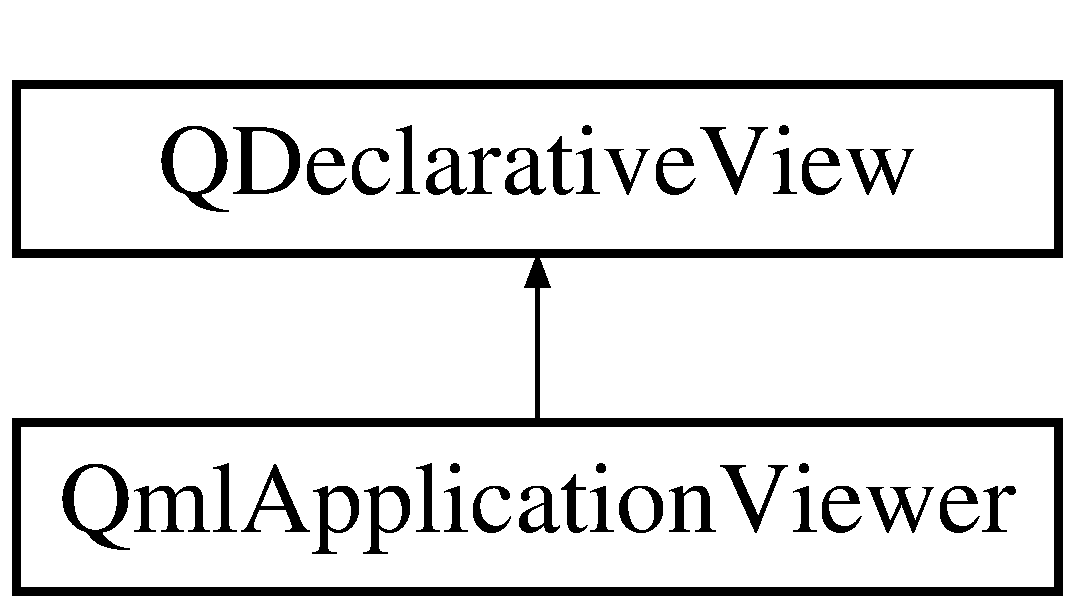
\includegraphics[height=2.000000cm]{classQmlApplicationViewer}
\end{center}
\end{figure}
\subsection*{Public Types}
\begin{DoxyCompactItemize}
\item 
enum \hyperlink{classQmlApplicationViewer_ac7c7e3771e785af566efd57ef319ac0b}{Screen\-Orientation} \{ \hyperlink{classQmlApplicationViewer_ac7c7e3771e785af566efd57ef319ac0baa2654139c60cbef50d0a8c21203b10f0}{Screen\-Orientation\-Lock\-Portrait}, 
\hyperlink{classQmlApplicationViewer_ac7c7e3771e785af566efd57ef319ac0ba7fb4a2bba3f8cd44a3fdd176a9409707}{Screen\-Orientation\-Lock\-Landscape}, 
\hyperlink{classQmlApplicationViewer_ac7c7e3771e785af566efd57ef319ac0ba43562095f1495c509eba50009e4fa8f0}{Screen\-Orientation\-Auto}
 \}
\end{DoxyCompactItemize}
\subsection*{Public Member Functions}
\begin{DoxyCompactItemize}
\item 
\hyperlink{classQmlApplicationViewer_a842902bbd62c77167410fd7676a8227c}{Qml\-Application\-Viewer} (Q\-Widget $\ast$parent=0)
\item 
virtual \hyperlink{classQmlApplicationViewer_ae712368928844f50f7d6ebe6481595e4}{$\sim$\-Qml\-Application\-Viewer} ()
\item 
void \hyperlink{classQmlApplicationViewer_a41240898c2e371e987fad66304f0acaf}{set\-Main\-Qml\-File} (const Q\-String \&file)
\item 
void \hyperlink{classQmlApplicationViewer_ae288e38be0964d47a08382056fe940c8}{add\-Import\-Path} (const Q\-String \&path)
\item 
void \hyperlink{classQmlApplicationViewer_a80f58eb6d6210437a5e788155a865169}{set\-Orientation} (\hyperlink{classQmlApplicationViewer_ac7c7e3771e785af566efd57ef319ac0b}{Screen\-Orientation} orientation)
\item 
void \hyperlink{classQmlApplicationViewer_ad899dc23f1a2c01276ec428db92215b8}{show\-Expanded} ()
\end{DoxyCompactItemize}
\subsection*{Static Public Member Functions}
\begin{DoxyCompactItemize}
\item 
static \hyperlink{classQmlApplicationViewer}{Qml\-Application\-Viewer} $\ast$ \hyperlink{classQmlApplicationViewer_a8287b2c20182a8dd7b60608f84dec496}{create} ()
\end{DoxyCompactItemize}


\subsection{Member Enumeration Documentation}
\hypertarget{classQmlApplicationViewer_ac7c7e3771e785af566efd57ef319ac0b}{\index{Qml\-Application\-Viewer@{Qml\-Application\-Viewer}!Screen\-Orientation@{Screen\-Orientation}}
\index{Screen\-Orientation@{Screen\-Orientation}!QmlApplicationViewer@{Qml\-Application\-Viewer}}
\subsubsection[{Screen\-Orientation}]{\setlength{\rightskip}{0pt plus 5cm}enum {\bf Qml\-Application\-Viewer\-::\-Screen\-Orientation}}}\label{classQmlApplicationViewer_ac7c7e3771e785af566efd57ef319ac0b}
\begin{Desc}
\item[Enumerator]\par
\begin{description}
\index{Screen\-Orientation\-Lock\-Portrait@{Screen\-Orientation\-Lock\-Portrait}!Qml\-Application\-Viewer@{Qml\-Application\-Viewer}}\index{Qml\-Application\-Viewer@{Qml\-Application\-Viewer}!Screen\-Orientation\-Lock\-Portrait@{Screen\-Orientation\-Lock\-Portrait}}\item[{\em 
\hypertarget{classQmlApplicationViewer_ac7c7e3771e785af566efd57ef319ac0baa2654139c60cbef50d0a8c21203b10f0}{Screen\-Orientation\-Lock\-Portrait}\label{classQmlApplicationViewer_ac7c7e3771e785af566efd57ef319ac0baa2654139c60cbef50d0a8c21203b10f0}
}]\index{Screen\-Orientation\-Lock\-Landscape@{Screen\-Orientation\-Lock\-Landscape}!Qml\-Application\-Viewer@{Qml\-Application\-Viewer}}\index{Qml\-Application\-Viewer@{Qml\-Application\-Viewer}!Screen\-Orientation\-Lock\-Landscape@{Screen\-Orientation\-Lock\-Landscape}}\item[{\em 
\hypertarget{classQmlApplicationViewer_ac7c7e3771e785af566efd57ef319ac0ba7fb4a2bba3f8cd44a3fdd176a9409707}{Screen\-Orientation\-Lock\-Landscape}\label{classQmlApplicationViewer_ac7c7e3771e785af566efd57ef319ac0ba7fb4a2bba3f8cd44a3fdd176a9409707}
}]\index{Screen\-Orientation\-Auto@{Screen\-Orientation\-Auto}!Qml\-Application\-Viewer@{Qml\-Application\-Viewer}}\index{Qml\-Application\-Viewer@{Qml\-Application\-Viewer}!Screen\-Orientation\-Auto@{Screen\-Orientation\-Auto}}\item[{\em 
\hypertarget{classQmlApplicationViewer_ac7c7e3771e785af566efd57ef319ac0ba43562095f1495c509eba50009e4fa8f0}{Screen\-Orientation\-Auto}\label{classQmlApplicationViewer_ac7c7e3771e785af566efd57ef319ac0ba43562095f1495c509eba50009e4fa8f0}
}]\end{description}
\end{Desc}


\subsection{Constructor \& Destructor Documentation}
\hypertarget{classQmlApplicationViewer_a842902bbd62c77167410fd7676a8227c}{\index{Qml\-Application\-Viewer@{Qml\-Application\-Viewer}!Qml\-Application\-Viewer@{Qml\-Application\-Viewer}}
\index{Qml\-Application\-Viewer@{Qml\-Application\-Viewer}!QmlApplicationViewer@{Qml\-Application\-Viewer}}
\subsubsection[{Qml\-Application\-Viewer}]{\setlength{\rightskip}{0pt plus 5cm}Qml\-Application\-Viewer\-::\-Qml\-Application\-Viewer (
\begin{DoxyParamCaption}
\item[{Q\-Widget $\ast$}]{parent = {\ttfamily 0}}
\end{DoxyParamCaption}
)\hspace{0.3cm}{\ttfamily [explicit]}}}\label{classQmlApplicationViewer_a842902bbd62c77167410fd7676a8227c}
\hypertarget{classQmlApplicationViewer_ae712368928844f50f7d6ebe6481595e4}{\index{Qml\-Application\-Viewer@{Qml\-Application\-Viewer}!$\sim$\-Qml\-Application\-Viewer@{$\sim$\-Qml\-Application\-Viewer}}
\index{$\sim$\-Qml\-Application\-Viewer@{$\sim$\-Qml\-Application\-Viewer}!QmlApplicationViewer@{Qml\-Application\-Viewer}}
\subsubsection[{$\sim$\-Qml\-Application\-Viewer}]{\setlength{\rightskip}{0pt plus 5cm}Qml\-Application\-Viewer\-::$\sim$\-Qml\-Application\-Viewer (
\begin{DoxyParamCaption}
{}
\end{DoxyParamCaption}
)\hspace{0.3cm}{\ttfamily [virtual]}}}\label{classQmlApplicationViewer_ae712368928844f50f7d6ebe6481595e4}


\subsection{Member Function Documentation}
\hypertarget{classQmlApplicationViewer_ae288e38be0964d47a08382056fe940c8}{\index{Qml\-Application\-Viewer@{Qml\-Application\-Viewer}!add\-Import\-Path@{add\-Import\-Path}}
\index{add\-Import\-Path@{add\-Import\-Path}!QmlApplicationViewer@{Qml\-Application\-Viewer}}
\subsubsection[{add\-Import\-Path}]{\setlength{\rightskip}{0pt plus 5cm}void Qml\-Application\-Viewer\-::add\-Import\-Path (
\begin{DoxyParamCaption}
\item[{const Q\-String \&}]{path}
\end{DoxyParamCaption}
)}}\label{classQmlApplicationViewer_ae288e38be0964d47a08382056fe940c8}
\hypertarget{classQmlApplicationViewer_a8287b2c20182a8dd7b60608f84dec496}{\index{Qml\-Application\-Viewer@{Qml\-Application\-Viewer}!create@{create}}
\index{create@{create}!QmlApplicationViewer@{Qml\-Application\-Viewer}}
\subsubsection[{create}]{\setlength{\rightskip}{0pt plus 5cm}{\bf Qml\-Application\-Viewer} $\ast$ Qml\-Application\-Viewer\-::create (
\begin{DoxyParamCaption}
{}
\end{DoxyParamCaption}
)\hspace{0.3cm}{\ttfamily [static]}}}\label{classQmlApplicationViewer_a8287b2c20182a8dd7b60608f84dec496}
\hypertarget{classQmlApplicationViewer_a41240898c2e371e987fad66304f0acaf}{\index{Qml\-Application\-Viewer@{Qml\-Application\-Viewer}!set\-Main\-Qml\-File@{set\-Main\-Qml\-File}}
\index{set\-Main\-Qml\-File@{set\-Main\-Qml\-File}!QmlApplicationViewer@{Qml\-Application\-Viewer}}
\subsubsection[{set\-Main\-Qml\-File}]{\setlength{\rightskip}{0pt plus 5cm}void Qml\-Application\-Viewer\-::set\-Main\-Qml\-File (
\begin{DoxyParamCaption}
\item[{const Q\-String \&}]{file}
\end{DoxyParamCaption}
)}}\label{classQmlApplicationViewer_a41240898c2e371e987fad66304f0acaf}
\hypertarget{classQmlApplicationViewer_a80f58eb6d6210437a5e788155a865169}{\index{Qml\-Application\-Viewer@{Qml\-Application\-Viewer}!set\-Orientation@{set\-Orientation}}
\index{set\-Orientation@{set\-Orientation}!QmlApplicationViewer@{Qml\-Application\-Viewer}}
\subsubsection[{set\-Orientation}]{\setlength{\rightskip}{0pt plus 5cm}void Qml\-Application\-Viewer\-::set\-Orientation (
\begin{DoxyParamCaption}
\item[{{\bf Screen\-Orientation}}]{orientation}
\end{DoxyParamCaption}
)}}\label{classQmlApplicationViewer_a80f58eb6d6210437a5e788155a865169}
\hypertarget{classQmlApplicationViewer_ad899dc23f1a2c01276ec428db92215b8}{\index{Qml\-Application\-Viewer@{Qml\-Application\-Viewer}!show\-Expanded@{show\-Expanded}}
\index{show\-Expanded@{show\-Expanded}!QmlApplicationViewer@{Qml\-Application\-Viewer}}
\subsubsection[{show\-Expanded}]{\setlength{\rightskip}{0pt plus 5cm}void Qml\-Application\-Viewer\-::show\-Expanded (
\begin{DoxyParamCaption}
{}
\end{DoxyParamCaption}
)}}\label{classQmlApplicationViewer_ad899dc23f1a2c01276ec428db92215b8}


The documentation for this class was generated from the following files\-:\begin{DoxyCompactItemize}
\item 
/media/philipjhj/\-Data/\-One\-Drive/\-Studie/\-Studenterprogrammør/\-S\-B\-S3/smartphonebrainscanner2-\/core/src/qmlapplicationviewer/\hyperlink{qmlapplicationviewer_8h}{qmlapplicationviewer.\-h}\item 
/media/philipjhj/\-Data/\-One\-Drive/\-Studie/\-Studenterprogrammør/\-S\-B\-S3/smartphonebrainscanner2-\/core/src/qmlapplicationviewer/\hyperlink{qmlapplicationviewer_8cpp}{qmlapplicationviewer.\-cpp}\end{DoxyCompactItemize}

\hypertarget{classQmlApplicationViewerPrivate}{\section{Qml\-Application\-Viewer\-Private Class Reference}
\label{classQmlApplicationViewerPrivate}\index{Qml\-Application\-Viewer\-Private@{Qml\-Application\-Viewer\-Private}}
}
\subsection*{Friends}
\begin{DoxyCompactItemize}
\item 
class \hyperlink{classQmlApplicationViewerPrivate_a7f82e38d9994cdd669ba61d3c5a76ccf}{Qml\-Application\-Viewer}
\end{DoxyCompactItemize}


\subsection{Friends And Related Function Documentation}
\hypertarget{classQmlApplicationViewerPrivate_a7f82e38d9994cdd669ba61d3c5a76ccf}{\index{Qml\-Application\-Viewer\-Private@{Qml\-Application\-Viewer\-Private}!Qml\-Application\-Viewer@{Qml\-Application\-Viewer}}
\index{Qml\-Application\-Viewer@{Qml\-Application\-Viewer}!QmlApplicationViewerPrivate@{Qml\-Application\-Viewer\-Private}}
\subsubsection[{Qml\-Application\-Viewer}]{\setlength{\rightskip}{0pt plus 5cm}friend class {\bf Qml\-Application\-Viewer}\hspace{0.3cm}{\ttfamily [friend]}}}\label{classQmlApplicationViewerPrivate_a7f82e38d9994cdd669ba61d3c5a76ccf}


The documentation for this class was generated from the following file\-:\begin{DoxyCompactItemize}
\item 
/media/philipjhj/\-Data/\-One\-Drive/\-Studie/\-Studenterprogrammør/\-S\-B\-S3/smartphonebrainscanner2-\/core/src/qmlapplicationviewer/\hyperlink{qmlapplicationviewer_8cpp}{qmlapplicationviewer.\-cpp}\end{DoxyCompactItemize}

\hypertarget{classJAMA_1_1QR}{\section{J\-A\-M\-A\-:\-:Q\-R$<$ Real $>$ Class Template Reference}
\label{classJAMA_1_1QR}\index{J\-A\-M\-A\-::\-Q\-R$<$ Real $>$@{J\-A\-M\-A\-::\-Q\-R$<$ Real $>$}}
}


{\ttfamily \#include $<$jama\-\_\-qr.\-h$>$}

\subsection*{Public Member Functions}
\begin{DoxyCompactItemize}
\item 
\hyperlink{classJAMA_1_1QR_a16e598f3853303908c9956801b2f4f9b}{Q\-R} (const \hyperlink{classTNT_1_1Array2D}{T\-N\-T\-::\-Array2\-D}$<$ Real $>$ \&A)
\item 
int \hyperlink{classJAMA_1_1QR_a0cd45f70cc469e03f8042583ecc1c073}{is\-Full\-Rank} () const 
\item 
\hyperlink{classTNT_1_1Array2D}{T\-N\-T\-::\-Array2\-D}$<$ Real $>$ \hyperlink{classJAMA_1_1QR_ab4492a1039efc813b129e08d7ffd630e}{get\-Householder} (void) const 
\item 
\hyperlink{classTNT_1_1Array2D}{T\-N\-T\-::\-Array2\-D}$<$ Real $>$ \hyperlink{classJAMA_1_1QR_adcc1fea05c9bfbe16eca617488809320}{get\-R} () const 
\item 
\hyperlink{classTNT_1_1Array2D}{T\-N\-T\-::\-Array2\-D}$<$ Real $>$ \hyperlink{classJAMA_1_1QR_af26cc81e42efdb4d46361b575e8c3f4b}{get\-Q} () const 
\item 
\hyperlink{classTNT_1_1Array1D}{T\-N\-T\-::\-Array1\-D}$<$ Real $>$ \hyperlink{classJAMA_1_1QR_ae21196cd1aeecad323ade468dd8d4af8}{solve} (const \hyperlink{classTNT_1_1Array1D}{T\-N\-T\-::\-Array1\-D}$<$ Real $>$ \&b) const 
\item 
\hyperlink{classTNT_1_1Array2D}{T\-N\-T\-::\-Array2\-D}$<$ Real $>$ \hyperlink{classJAMA_1_1QR_a48cbe600fd6a8754a33fc382fc16d2a9}{solve} (const \hyperlink{classTNT_1_1Array2D}{T\-N\-T\-::\-Array2\-D}$<$ Real $>$ \&B) const 
\end{DoxyCompactItemize}


\subsection{Detailed Description}
\subsubsection*{template$<$class Real$>$class J\-A\-M\-A\-::\-Q\-R$<$ Real $>$}

Classical \hyperlink{classJAMA_1_1QR}{Q\-R} Decompisition\-: for an m-\/by-\/n matrix A with m $>$= n, the \hyperlink{classJAMA_1_1QR}{Q\-R} decomposition is an m-\/by-\/n orthogonal matrix Q and an n-\/by-\/n upper triangular matrix R so that A = Q$\ast$\-R. 

The \hyperlink{classJAMA_1_1QR}{Q\-R} decompostion always exists, even if the matrix does not have full rank, so the constructor will never fail. The primary use of the \hyperlink{classJAMA_1_1QR}{Q\-R} decomposition is in the least squares solution of nonsquare systems of simultaneous linear equations. This will fail if \hyperlink{classJAMA_1_1QR_a0cd45f70cc469e03f8042583ecc1c073}{is\-Full\-Rank()} returns 0 (false).

The Q and R factors can be retrived via the \hyperlink{classJAMA_1_1QR_af26cc81e42efdb4d46361b575e8c3f4b}{get\-Q()} and \hyperlink{classJAMA_1_1QR_adcc1fea05c9bfbe16eca617488809320}{get\-R()} methods. Furthermore, a \hyperlink{classJAMA_1_1QR_ae21196cd1aeecad323ade468dd8d4af8}{solve()} method is provided to find the least squares solution of Ax=b using the \hyperlink{classJAMA_1_1QR}{Q\-R} factors.

(Adapted from \hyperlink{namespaceJAMA}{J\-A\-M\-A}, a Java Matrix Library, developed by jointly by the Mathworks and N\-I\-S\-T; see \href{http://math.nist.gov/javanumerics/jama}{\tt http\-://math.\-nist.\-gov/javanumerics/jama}). 

\subsection{Constructor \& Destructor Documentation}
\hypertarget{classJAMA_1_1QR_a16e598f3853303908c9956801b2f4f9b}{\index{J\-A\-M\-A\-::\-Q\-R@{J\-A\-M\-A\-::\-Q\-R}!Q\-R@{Q\-R}}
\index{Q\-R@{Q\-R}!JAMA::QR@{J\-A\-M\-A\-::\-Q\-R}}
\subsubsection[{Q\-R}]{\setlength{\rightskip}{0pt plus 5cm}template$<$class Real $>$ {\bf J\-A\-M\-A\-::\-Q\-R}$<$ Real $>$\-::{\bf Q\-R} (
\begin{DoxyParamCaption}
\item[{const {\bf T\-N\-T\-::\-Array2\-D}$<$ Real $>$ \&}]{A}
\end{DoxyParamCaption}
)\hspace{0.3cm}{\ttfamily [inline]}}}\label{classJAMA_1_1QR_a16e598f3853303908c9956801b2f4f9b}
Create a \hyperlink{classJAMA_1_1QR}{Q\-R} factorization object for A.


\begin{DoxyParams}{Parameters}
{\em A} & rectangular (m$>$=n) matrix. \\
\hline
\end{DoxyParams}


\subsection{Member Function Documentation}
\hypertarget{classJAMA_1_1QR_ab4492a1039efc813b129e08d7ffd630e}{\index{J\-A\-M\-A\-::\-Q\-R@{J\-A\-M\-A\-::\-Q\-R}!get\-Householder@{get\-Householder}}
\index{get\-Householder@{get\-Householder}!JAMA::QR@{J\-A\-M\-A\-::\-Q\-R}}
\subsubsection[{get\-Householder}]{\setlength{\rightskip}{0pt plus 5cm}template$<$class Real $>$ {\bf T\-N\-T\-::\-Array2\-D}$<$Real$>$ {\bf J\-A\-M\-A\-::\-Q\-R}$<$ Real $>$\-::get\-Householder (
\begin{DoxyParamCaption}
\item[{void}]{}
\end{DoxyParamCaption}
) const\hspace{0.3cm}{\ttfamily [inline]}}}\label{classJAMA_1_1QR_ab4492a1039efc813b129e08d7ffd630e}
Retreive the Householder vectors from \hyperlink{classJAMA_1_1QR}{Q\-R} factorization \begin{DoxyReturn}{Returns}
lower trapezoidal matrix whose columns define the reflections 
\end{DoxyReturn}
\hypertarget{classJAMA_1_1QR_af26cc81e42efdb4d46361b575e8c3f4b}{\index{J\-A\-M\-A\-::\-Q\-R@{J\-A\-M\-A\-::\-Q\-R}!get\-Q@{get\-Q}}
\index{get\-Q@{get\-Q}!JAMA::QR@{J\-A\-M\-A\-::\-Q\-R}}
\subsubsection[{get\-Q}]{\setlength{\rightskip}{0pt plus 5cm}template$<$class Real $>$ {\bf T\-N\-T\-::\-Array2\-D}$<$Real$>$ {\bf J\-A\-M\-A\-::\-Q\-R}$<$ Real $>$\-::get\-Q (
\begin{DoxyParamCaption}
{}
\end{DoxyParamCaption}
) const\hspace{0.3cm}{\ttfamily [inline]}}}\label{classJAMA_1_1QR_af26cc81e42efdb4d46361b575e8c3f4b}
Generate and return the (economy-\/sized) orthogonal factor 
\begin{DoxyParams}{Parameters}
{\em Q} & the (ecnomy-\/sized) orthogonal factor (Q$\ast$\-R=A). \\
\hline
\end{DoxyParams}
\hypertarget{classJAMA_1_1QR_adcc1fea05c9bfbe16eca617488809320}{\index{J\-A\-M\-A\-::\-Q\-R@{J\-A\-M\-A\-::\-Q\-R}!get\-R@{get\-R}}
\index{get\-R@{get\-R}!JAMA::QR@{J\-A\-M\-A\-::\-Q\-R}}
\subsubsection[{get\-R}]{\setlength{\rightskip}{0pt plus 5cm}template$<$class Real $>$ {\bf T\-N\-T\-::\-Array2\-D}$<$Real$>$ {\bf J\-A\-M\-A\-::\-Q\-R}$<$ Real $>$\-::get\-R (
\begin{DoxyParamCaption}
{}
\end{DoxyParamCaption}
) const\hspace{0.3cm}{\ttfamily [inline]}}}\label{classJAMA_1_1QR_adcc1fea05c9bfbe16eca617488809320}
Return the upper triangular factor, R, of the \hyperlink{classJAMA_1_1QR}{Q\-R} factorization \begin{DoxyReturn}{Returns}
R 
\end{DoxyReturn}
\hypertarget{classJAMA_1_1QR_a0cd45f70cc469e03f8042583ecc1c073}{\index{J\-A\-M\-A\-::\-Q\-R@{J\-A\-M\-A\-::\-Q\-R}!is\-Full\-Rank@{is\-Full\-Rank}}
\index{is\-Full\-Rank@{is\-Full\-Rank}!JAMA::QR@{J\-A\-M\-A\-::\-Q\-R}}
\subsubsection[{is\-Full\-Rank}]{\setlength{\rightskip}{0pt plus 5cm}template$<$class Real $>$ int {\bf J\-A\-M\-A\-::\-Q\-R}$<$ Real $>$\-::is\-Full\-Rank (
\begin{DoxyParamCaption}
{}
\end{DoxyParamCaption}
) const\hspace{0.3cm}{\ttfamily [inline]}}}\label{classJAMA_1_1QR_a0cd45f70cc469e03f8042583ecc1c073}
Flag to denote the matrix is of full rank.

\begin{DoxyReturn}{Returns}
1 if matrix is full rank, 0 otherwise. 
\end{DoxyReturn}
\hypertarget{classJAMA_1_1QR_ae21196cd1aeecad323ade468dd8d4af8}{\index{J\-A\-M\-A\-::\-Q\-R@{J\-A\-M\-A\-::\-Q\-R}!solve@{solve}}
\index{solve@{solve}!JAMA::QR@{J\-A\-M\-A\-::\-Q\-R}}
\subsubsection[{solve}]{\setlength{\rightskip}{0pt plus 5cm}template$<$class Real $>$ {\bf T\-N\-T\-::\-Array1\-D}$<$Real$>$ {\bf J\-A\-M\-A\-::\-Q\-R}$<$ Real $>$\-::solve (
\begin{DoxyParamCaption}
\item[{const {\bf T\-N\-T\-::\-Array1\-D}$<$ Real $>$ \&}]{b}
\end{DoxyParamCaption}
) const\hspace{0.3cm}{\ttfamily [inline]}}}\label{classJAMA_1_1QR_ae21196cd1aeecad323ade468dd8d4af8}
Least squares solution of A$\ast$x = b 
\begin{DoxyParams}{Parameters}
{\em B} & m-\/length array (vector). \\
\hline
\end{DoxyParams}
\begin{DoxyReturn}{Returns}
x n-\/length array (vector) that minimizes the two norm of Q$\ast$\-R$\ast$\-X-\/\-B. If B is non-\/conformant, or if \hyperlink{classJAMA_1_1QR_a0cd45f70cc469e03f8042583ecc1c073}{Q\-R.\-is\-Full\-Rank()} is false, the routine returns a null (0-\/length) vector. 
\end{DoxyReturn}
\hypertarget{classJAMA_1_1QR_a48cbe600fd6a8754a33fc382fc16d2a9}{\index{J\-A\-M\-A\-::\-Q\-R@{J\-A\-M\-A\-::\-Q\-R}!solve@{solve}}
\index{solve@{solve}!JAMA::QR@{J\-A\-M\-A\-::\-Q\-R}}
\subsubsection[{solve}]{\setlength{\rightskip}{0pt plus 5cm}template$<$class Real $>$ {\bf T\-N\-T\-::\-Array2\-D}$<$Real$>$ {\bf J\-A\-M\-A\-::\-Q\-R}$<$ Real $>$\-::solve (
\begin{DoxyParamCaption}
\item[{const {\bf T\-N\-T\-::\-Array2\-D}$<$ Real $>$ \&}]{B}
\end{DoxyParamCaption}
) const\hspace{0.3cm}{\ttfamily [inline]}}}\label{classJAMA_1_1QR_a48cbe600fd6a8754a33fc382fc16d2a9}
Least squares solution of A$\ast$\-X = B 
\begin{DoxyParams}{Parameters}
{\em B} & m x k Array (must conform). \\
\hline
\end{DoxyParams}
\begin{DoxyReturn}{Returns}
X n x k Array that minimizes the two norm of Q$\ast$\-R$\ast$\-X-\/\-B. If B is non-\/conformant, or if \hyperlink{classJAMA_1_1QR_a0cd45f70cc469e03f8042583ecc1c073}{Q\-R.\-is\-Full\-Rank()} is false, the routine returns a null (0x0) array. 
\end{DoxyReturn}


The documentation for this class was generated from the following file\-:\begin{DoxyCompactItemize}
\item 
/media/philipjhj/\-Data/\-One\-Drive/\-Studie/\-Studenterprogrammør/\-S\-B\-S3/smartphonebrainscanner2-\/core/src/jama125/\hyperlink{jama__qr_8h}{jama\-\_\-qr.\-h}\end{DoxyCompactItemize}

\hypertarget{classSbs2Callback}{\section{Sbs2\-Callback Class Reference}
\label{classSbs2Callback}\index{Sbs2\-Callback@{Sbs2\-Callback}}
}


{\ttfamily \#include $<$sbs2callback.\-h$>$}

Inheritance diagram for Sbs2\-Callback\-:\begin{figure}[H]
\begin{center}
\leavevmode
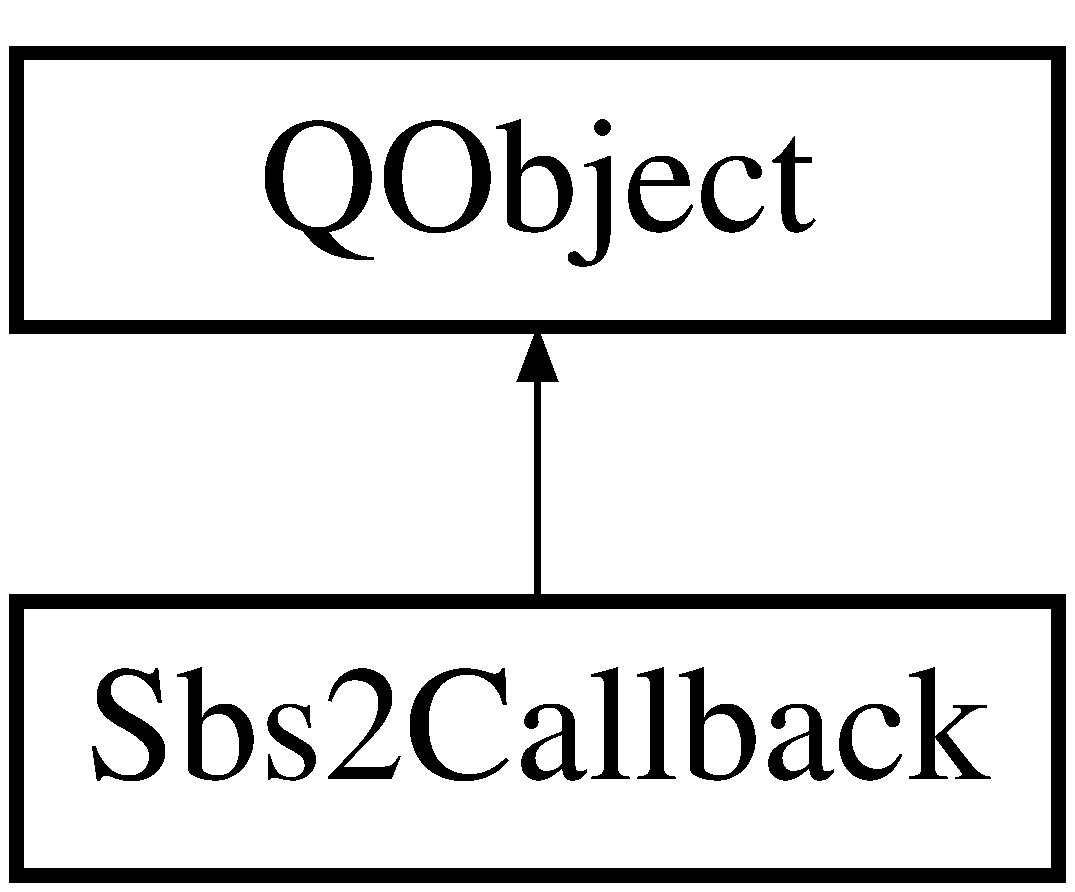
\includegraphics[height=2.000000cm]{classSbs2Callback}
\end{center}
\end{figure}
\subsection*{Public Slots}
\begin{DoxyCompactItemize}
\item 
void \hyperlink{classSbs2Callback_a7d5a8d24240c64c58d79be03d990526b}{start\-Recording} (Q\-String user, Q\-String description)
\item 
void \hyperlink{classSbs2Callback_a62cf46e7415db4cafd2dad2d0b821a42}{stop\-Recording} ()
\item 
void \hyperlink{classSbs2Callback_a18e265de74d9a4e46a0ec3b1b4064a39}{insert\-Into\-Meta\-File} (Q\-String event)
\item 
void \hyperlink{classSbs2Callback_a398880b41625e91557827f3375cfc835}{turn\-Filter\-On} (int fband\-Low\-\_\-, int fband\-High\-\_\-, int filter\-Order\-\_\-)
\item 
void \hyperlink{classSbs2Callback_a0887db578eeafa6056ab8a5ae413ff16}{turn\-Filter\-Off} ()
\item 
void \hyperlink{classSbs2Callback_a3cb61e2d70abbf73d546a8329863b331}{turn\-Channel\-Spectrogram\-On} (int spectrogram\-Channel\-Samples\-\_\-=128, int spectrogram\-Channel\-Length\-\_\-=128, int spectrogram\-Channel\-Delta\-\_\-=0)
\item 
void \hyperlink{classSbs2Callback_a7a05a0cca91ec4ac82387f7813f8dce0}{turn\-Channel\-Spectrogram\-Off} ()
\item 
void \hyperlink{classSbs2Callback_a4120c9ad061934c2c3ba9e12fad19fa3}{set\-Window\-Type} (\hyperlink{classSbs2Spectrogram_a22265347883488b8385c83b67882d915}{Sbs2\-Spectrogram\-::\-Window\-Type} window\-Type)
\item 
void \hyperlink{classSbs2Callback_a503b955e5f769de0441c03aca7119d39}{set\-Window\-Type} (int window\-Type)
\item 
void \hyperlink{classSbs2Callback_a9a7e91c47226e2110c5592f3216c8ec4}{turn\-On\-Source\-Reconstruction\-Loreta} (int source\-Reconstruction\-Samples\-\_\-, int source\-Reconstruction\-Delta\-\_\-, int source\-Reconstruction\-Model\-Update\-Length\-\_\-, int source\-Reconstruction\-Model\-Update\-Delta\-\_\-, Q\-String hardware\-\_\-=\char`\"{}emotiv\char`\"{})
\item 
void \hyperlink{classSbs2Callback_a1dc541c041e8ec86c4e2c11aed3dc137}{turn\-On\-Source\-Reconstructio\-Sparse} (int source\-Reconstruction\-Samples, Q\-Vector$<$ double $>$ lambdas, Q\-String hardware=\char`\"{}emotiv\char`\"{})
\item 
void \hyperlink{classSbs2Callback_ad6b505b02b39d1c55a766d9965f6cbca}{spectrogram\-Updated\-Slot} ()
\item 
void \hyperlink{classSbs2Callback_a25ed563d5af289e5edf97a954dad0955}{set\-Hardware} (Q\-String hardware)
\item 
void \hyperlink{classSbs2Callback_a79ef4e00ba8d0ea228c588b321a6d9d1}{turn\-Send\-Raw\-Data\-On} (Q\-String raw\-Data\-Server\-Address\-\_\-, int raw\-Data\-Port\-\_\-, int raw\-Data\-Size\-\_\-=32, int raw\-Data\-Queue\-Length\-\_\-=8)
\item 
void \hyperlink{classSbs2Callback_ab8aa8c77bcfc660ead0c3bd5c9771ba7}{turn\-Send\-Raw\-Data\-Off} ()
\item 
void \hyperlink{classSbs2Callback_afed7146f24d2d0fbea4413f36689cd1e}{add\-Raw\-Data\-Host} (Q\-String address, int port)
\item 
void \hyperlink{classSbs2Callback_a63e6d9a736d558abf7d4b32527deab7b}{remove\-Raw\-Data\-Host} (Q\-String address, int port)
\item 
void \hyperlink{classSbs2Callback_a84e65bd6c98a739c5ff13afe640e2b0d}{send\-Message} (Q\-String message, Q\-String address, int port)
\item 
void \hyperlink{classSbs2Callback_a5f5c224b7876314c5a9fd57e85e84b54}{send\-Message} (Q\-String message)
\item 
void \hyperlink{classSbs2Callback_aded5f0084d59d3361d939684bd7a34e2}{add\-Message\-Udp\-Output\-Host} (Q\-String address, int port)
\item 
void \hyperlink{classSbs2Callback_afffe41163a5e4e1e7a3a2cc428946d49}{remove\-Message\-Udp\-Output\-Host} (Q\-String address)
\item 
void \hyperlink{classSbs2Callback_af6a1b32d8d4eddad9fef9c784569dc1b}{clear\-Message\-Udp\-Output\-Hosts} ()
\item 
void \hyperlink{classSbs2Callback_a233b2be700ec8c7044f2f24d73825966}{turn\-Receive\-Message\-On} (Q\-String address, int port)
\item 
void \hyperlink{classSbs2Callback_aefcdc819e629bf05240cfa3ed3eeabb5}{turn\-Receive\-Message\-Off} ()
\item 
void \hyperlink{classSbs2Callback_aa8e69a7685705f41f0e3ee288af4f899}{read\-Message} (Q\-String data, Q\-String sender, int sender\-Port)
\item 
void \hyperlink{classSbs2Callback_a6ab3cb55cc737a7797a3c310d3c51154}{get\-Network\-Addresses} ()
\item 
void \hyperlink{classSbs2Callback_a2a51dea2e8d72a184b612b8545ecd341}{device\-Found} (Q\-Map$<$ Q\-String, Q\-Variant $>$ params\-\_\-)
\end{DoxyCompactItemize}
\subsection*{Signals}
\begin{DoxyCompactItemize}
\item 
void \hyperlink{classSbs2Callback_a5184124613eada5520f1a3a170004a2b}{time\-Tick10} ()
\item 
void \hyperlink{classSbs2Callback_ad2664cc07b84a0bf32853d8b73a33269}{time\-Tick2} ()
\item 
void \hyperlink{classSbs2Callback_afc2ede902add0f774b75fd6180c4d2f6}{time\-Tick4} ()
\item 
void \hyperlink{classSbs2Callback_a97bab20747140c597618f804b6228072}{time\-Tick8} ()
\item 
void \hyperlink{classSbs2Callback_a61ec73d9af8b810f81eda4d953a7d514}{time\-Tick0} ()
\item 
void \hyperlink{classSbs2Callback_aadf4b16079f8dcadbd09b3469682092f}{time\-Tick16} ()
\item 
void \hyperlink{classSbs2Callback_ad3bb5730a00149ba4b72342050aaf0a6}{set\-Window\-Type\-Signal} (\hyperlink{classSbs2Spectrogram_a22265347883488b8385c83b67882d915}{Sbs2\-Spectrogram\-::\-Window\-Type} window\-Type)
\item 
void \hyperlink{classSbs2Callback_ab6e4c13c9062855f656df9ceed5cd043}{battery\-Value} (Q\-Variant value)
\item 
void \hyperlink{classSbs2Callback_a06f6ee83c0568d015737115c1bda0c35}{cq\-Values} (Q\-Variant channel, Q\-Variant value)
\item 
void \hyperlink{classSbs2Callback_a234ed679eb92e8d74a570fe6b212ac01}{cq\-Value} (Q\-String channel, double value)
\item 
void \hyperlink{classSbs2Callback_aad050bf9599c2adce3d7a40e635da9ad}{spectrogram\-Updated} ()
\item 
void \hyperlink{classSbs2Callback_a2f0493b36e4cf02f621f0a4a5867f30e}{udp\-Message\-Received} (Q\-String data, Q\-String sender, int port)
\item 
void \hyperlink{classSbs2Callback_a3f36470fea877fef65f50f0b6c123e10}{network\-Addresses} (Q\-Variant data)
\item 
void \hyperlink{classSbs2Callback_ac03ad51c29e3ed87d6ddca27422f594a}{hardware\-Changed} (Q\-String hardware)
\item 
void \hyperlink{classSbs2Callback_af2630321eef9e48a74e3d4029513117c}{device\-Found\-Signal} (Q\-Map$<$ Q\-String, Q\-Variant $>$ \hyperlink{classSbs2Callback_acd4a65e3bee2e9a1f9ceccd9cfbd17be}{params})
\end{DoxyCompactItemize}
\subsection*{Public Member Functions}
\begin{DoxyCompactItemize}
\item 
\hyperlink{classSbs2Callback_a98a3e60515fae31413710bb4364532e8}{Sbs2\-Callback} (Q\-Object $\ast$parent=0)
\item 
virtual void \hyperlink{classSbs2Callback_a5a8ca18e20621369676d2fc574560591}{get\-Data} (\hyperlink{classSbs2Packet}{Sbs2\-Packet} $\ast$packet)
\item 
Q\-String \hyperlink{classSbs2Callback_ae3266d38f8f2b37fd89861e7d80f1b29}{get\-Raw\-Filename} ()
\end{DoxyCompactItemize}
\subsection*{Static Public Member Functions}
\begin{DoxyCompactItemize}
\item 
static int \hyperlink{classSbs2Callback_ae3947414f7194c7f7fd7339bfaf8b482}{get\-Current\-Packet\-Counter} ()
\item 
static int \hyperlink{classSbs2Callback_abe16322e2f43f576217c4f32695cdbdf}{get\-Current\-Packet} ()
\end{DoxyCompactItemize}
\subsection*{Protected Member Functions}
\begin{DoxyCompactItemize}
\item 
void \hyperlink{classSbs2Callback_a9379f04332bd3d3715a1604a153d4ccd}{set\-Packet} (\hyperlink{classSbs2Packet}{Sbs2\-Packet} $\ast$packet)
\item 
void \hyperlink{classSbs2Callback_a3f8f597a4d8db5a417c5087aa2ccde2c}{set\-Sbs2\-Data\-Handler} (\hyperlink{classSbs2DataHandler}{Sbs2\-Data\-Handler} $\ast$sbs2\-Data\-Handler\-\_\-)
\end{DoxyCompactItemize}
\subsection*{Protected Attributes}
\begin{DoxyCompactItemize}
\item 
\hyperlink{classSbs2DataHandler}{Sbs2\-Data\-Handler} $\ast$ \hyperlink{classSbs2Callback_abb8a77a313b6def9350f6650d45e4712}{sbs2\-Data\-Handler}
\item 
int \hyperlink{classSbs2Callback_a8421999c9a01bf911680ea662420e924}{samples\-Collected}
\item 
\hyperlink{classSbs2Packet}{Sbs2\-Packet} $\ast$ \hyperlink{classSbs2Callback_ad363232a631f5af946b190b4fa7183af}{this\-Packet}
\item 
\hyperlink{classSbs2Region}{Sbs2\-Region} $\ast$ \hyperlink{classSbs2Callback_aa9560af6052c4c738b77ecf60c5cf84b}{sbs2\-Region}
\item 
int \hyperlink{classSbs2Callback_a2c34fb4b056259272d30dc1003539a00}{is\-Recording}
\item 
Q\-Map$<$ Q\-String, Q\-Variant $>$ \hyperlink{classSbs2Callback_acd4a65e3bee2e9a1f9ceccd9cfbd17be}{params}
\item 
int \hyperlink{classSbs2Callback_ae41fef7a11c79e479f4645e25ece06d5}{device\-Present}
\end{DoxyCompactItemize}
\subsection*{Static Protected Attributes}
\begin{DoxyCompactItemize}
\item 
static int \hyperlink{classSbs2Callback_a7af1072fbca19a0439dc5c6bcb4da665}{current\-Packet\-Counter} = 0
\item 
static int \hyperlink{classSbs2Callback_ab9bbbc2d9a06c2200d428f84703134bd}{current\-Packet} = 0
\end{DoxyCompactItemize}


\subsection{Constructor \& Destructor Documentation}
\hypertarget{classSbs2Callback_a98a3e60515fae31413710bb4364532e8}{\index{Sbs2\-Callback@{Sbs2\-Callback}!Sbs2\-Callback@{Sbs2\-Callback}}
\index{Sbs2\-Callback@{Sbs2\-Callback}!Sbs2Callback@{Sbs2\-Callback}}
\subsubsection[{Sbs2\-Callback}]{\setlength{\rightskip}{0pt plus 5cm}Sbs2\-Callback\-::\-Sbs2\-Callback (
\begin{DoxyParamCaption}
\item[{Q\-Object $\ast$}]{parent = {\ttfamily 0}}
\end{DoxyParamCaption}
)\hspace{0.3cm}{\ttfamily [explicit]}}}\label{classSbs2Callback_a98a3e60515fae31413710bb4364532e8}


\subsection{Member Function Documentation}
\hypertarget{classSbs2Callback_aded5f0084d59d3361d939684bd7a34e2}{\index{Sbs2\-Callback@{Sbs2\-Callback}!add\-Message\-Udp\-Output\-Host@{add\-Message\-Udp\-Output\-Host}}
\index{add\-Message\-Udp\-Output\-Host@{add\-Message\-Udp\-Output\-Host}!Sbs2Callback@{Sbs2\-Callback}}
\subsubsection[{add\-Message\-Udp\-Output\-Host}]{\setlength{\rightskip}{0pt plus 5cm}void Sbs2\-Callback\-::add\-Message\-Udp\-Output\-Host (
\begin{DoxyParamCaption}
\item[{Q\-String}]{address, }
\item[{int}]{port}
\end{DoxyParamCaption}
)\hspace{0.3cm}{\ttfamily [slot]}}}\label{classSbs2Callback_aded5f0084d59d3361d939684bd7a34e2}
\hypertarget{classSbs2Callback_afed7146f24d2d0fbea4413f36689cd1e}{\index{Sbs2\-Callback@{Sbs2\-Callback}!add\-Raw\-Data\-Host@{add\-Raw\-Data\-Host}}
\index{add\-Raw\-Data\-Host@{add\-Raw\-Data\-Host}!Sbs2Callback@{Sbs2\-Callback}}
\subsubsection[{add\-Raw\-Data\-Host}]{\setlength{\rightskip}{0pt plus 5cm}void Sbs2\-Callback\-::add\-Raw\-Data\-Host (
\begin{DoxyParamCaption}
\item[{Q\-String}]{address, }
\item[{int}]{port}
\end{DoxyParamCaption}
)\hspace{0.3cm}{\ttfamily [slot]}}}\label{classSbs2Callback_afed7146f24d2d0fbea4413f36689cd1e}
\hypertarget{classSbs2Callback_ab6e4c13c9062855f656df9ceed5cd043}{\index{Sbs2\-Callback@{Sbs2\-Callback}!battery\-Value@{battery\-Value}}
\index{battery\-Value@{battery\-Value}!Sbs2Callback@{Sbs2\-Callback}}
\subsubsection[{battery\-Value}]{\setlength{\rightskip}{0pt plus 5cm}void Sbs2\-Callback\-::battery\-Value (
\begin{DoxyParamCaption}
\item[{Q\-Variant}]{value}
\end{DoxyParamCaption}
)\hspace{0.3cm}{\ttfamily [signal]}}}\label{classSbs2Callback_ab6e4c13c9062855f656df9ceed5cd043}
\hypertarget{classSbs2Callback_af6a1b32d8d4eddad9fef9c784569dc1b}{\index{Sbs2\-Callback@{Sbs2\-Callback}!clear\-Message\-Udp\-Output\-Hosts@{clear\-Message\-Udp\-Output\-Hosts}}
\index{clear\-Message\-Udp\-Output\-Hosts@{clear\-Message\-Udp\-Output\-Hosts}!Sbs2Callback@{Sbs2\-Callback}}
\subsubsection[{clear\-Message\-Udp\-Output\-Hosts}]{\setlength{\rightskip}{0pt plus 5cm}void Sbs2\-Callback\-::clear\-Message\-Udp\-Output\-Hosts (
\begin{DoxyParamCaption}
{}
\end{DoxyParamCaption}
)\hspace{0.3cm}{\ttfamily [slot]}}}\label{classSbs2Callback_af6a1b32d8d4eddad9fef9c784569dc1b}
\hypertarget{classSbs2Callback_a234ed679eb92e8d74a570fe6b212ac01}{\index{Sbs2\-Callback@{Sbs2\-Callback}!cq\-Value@{cq\-Value}}
\index{cq\-Value@{cq\-Value}!Sbs2Callback@{Sbs2\-Callback}}
\subsubsection[{cq\-Value}]{\setlength{\rightskip}{0pt plus 5cm}void Sbs2\-Callback\-::cq\-Value (
\begin{DoxyParamCaption}
\item[{Q\-String}]{channel, }
\item[{double}]{value}
\end{DoxyParamCaption}
)\hspace{0.3cm}{\ttfamily [signal]}}}\label{classSbs2Callback_a234ed679eb92e8d74a570fe6b212ac01}
\hypertarget{classSbs2Callback_a06f6ee83c0568d015737115c1bda0c35}{\index{Sbs2\-Callback@{Sbs2\-Callback}!cq\-Values@{cq\-Values}}
\index{cq\-Values@{cq\-Values}!Sbs2Callback@{Sbs2\-Callback}}
\subsubsection[{cq\-Values}]{\setlength{\rightskip}{0pt plus 5cm}void Sbs2\-Callback\-::cq\-Values (
\begin{DoxyParamCaption}
\item[{Q\-Variant}]{channel, }
\item[{Q\-Variant}]{value}
\end{DoxyParamCaption}
)\hspace{0.3cm}{\ttfamily [signal]}}}\label{classSbs2Callback_a06f6ee83c0568d015737115c1bda0c35}
\hypertarget{classSbs2Callback_a2a51dea2e8d72a184b612b8545ecd341}{\index{Sbs2\-Callback@{Sbs2\-Callback}!device\-Found@{device\-Found}}
\index{device\-Found@{device\-Found}!Sbs2Callback@{Sbs2\-Callback}}
\subsubsection[{device\-Found}]{\setlength{\rightskip}{0pt plus 5cm}void Sbs2\-Callback\-::device\-Found (
\begin{DoxyParamCaption}
\item[{Q\-Map$<$ Q\-String, Q\-Variant $>$}]{params\-\_\-}
\end{DoxyParamCaption}
)\hspace{0.3cm}{\ttfamily [slot]}}}\label{classSbs2Callback_a2a51dea2e8d72a184b612b8545ecd341}
\hypertarget{classSbs2Callback_af2630321eef9e48a74e3d4029513117c}{\index{Sbs2\-Callback@{Sbs2\-Callback}!device\-Found\-Signal@{device\-Found\-Signal}}
\index{device\-Found\-Signal@{device\-Found\-Signal}!Sbs2Callback@{Sbs2\-Callback}}
\subsubsection[{device\-Found\-Signal}]{\setlength{\rightskip}{0pt plus 5cm}void Sbs2\-Callback\-::device\-Found\-Signal (
\begin{DoxyParamCaption}
\item[{Q\-Map$<$ Q\-String, Q\-Variant $>$}]{params}
\end{DoxyParamCaption}
)\hspace{0.3cm}{\ttfamily [signal]}}}\label{classSbs2Callback_af2630321eef9e48a74e3d4029513117c}
\hypertarget{classSbs2Callback_abe16322e2f43f576217c4f32695cdbdf}{\index{Sbs2\-Callback@{Sbs2\-Callback}!get\-Current\-Packet@{get\-Current\-Packet}}
\index{get\-Current\-Packet@{get\-Current\-Packet}!Sbs2Callback@{Sbs2\-Callback}}
\subsubsection[{get\-Current\-Packet}]{\setlength{\rightskip}{0pt plus 5cm}int Sbs2\-Callback\-::get\-Current\-Packet (
\begin{DoxyParamCaption}
{}
\end{DoxyParamCaption}
)\hspace{0.3cm}{\ttfamily [static]}}}\label{classSbs2Callback_abe16322e2f43f576217c4f32695cdbdf}
\hypertarget{classSbs2Callback_ae3947414f7194c7f7fd7339bfaf8b482}{\index{Sbs2\-Callback@{Sbs2\-Callback}!get\-Current\-Packet\-Counter@{get\-Current\-Packet\-Counter}}
\index{get\-Current\-Packet\-Counter@{get\-Current\-Packet\-Counter}!Sbs2Callback@{Sbs2\-Callback}}
\subsubsection[{get\-Current\-Packet\-Counter}]{\setlength{\rightskip}{0pt plus 5cm}int Sbs2\-Callback\-::get\-Current\-Packet\-Counter (
\begin{DoxyParamCaption}
{}
\end{DoxyParamCaption}
)\hspace{0.3cm}{\ttfamily [static]}}}\label{classSbs2Callback_ae3947414f7194c7f7fd7339bfaf8b482}
\hypertarget{classSbs2Callback_a5a8ca18e20621369676d2fc574560591}{\index{Sbs2\-Callback@{Sbs2\-Callback}!get\-Data@{get\-Data}}
\index{get\-Data@{get\-Data}!Sbs2Callback@{Sbs2\-Callback}}
\subsubsection[{get\-Data}]{\setlength{\rightskip}{0pt plus 5cm}virtual void Sbs2\-Callback\-::get\-Data (
\begin{DoxyParamCaption}
\item[{{\bf Sbs2\-Packet} $\ast$}]{packet}
\end{DoxyParamCaption}
)\hspace{0.3cm}{\ttfamily [inline]}, {\ttfamily [virtual]}}}\label{classSbs2Callback_a5a8ca18e20621369676d2fc574560591}
\hypertarget{classSbs2Callback_a6ab3cb55cc737a7797a3c310d3c51154}{\index{Sbs2\-Callback@{Sbs2\-Callback}!get\-Network\-Addresses@{get\-Network\-Addresses}}
\index{get\-Network\-Addresses@{get\-Network\-Addresses}!Sbs2Callback@{Sbs2\-Callback}}
\subsubsection[{get\-Network\-Addresses}]{\setlength{\rightskip}{0pt plus 5cm}void Sbs2\-Callback\-::get\-Network\-Addresses (
\begin{DoxyParamCaption}
{}
\end{DoxyParamCaption}
)\hspace{0.3cm}{\ttfamily [slot]}}}\label{classSbs2Callback_a6ab3cb55cc737a7797a3c310d3c51154}
\hypertarget{classSbs2Callback_ae3266d38f8f2b37fd89861e7d80f1b29}{\index{Sbs2\-Callback@{Sbs2\-Callback}!get\-Raw\-Filename@{get\-Raw\-Filename}}
\index{get\-Raw\-Filename@{get\-Raw\-Filename}!Sbs2Callback@{Sbs2\-Callback}}
\subsubsection[{get\-Raw\-Filename}]{\setlength{\rightskip}{0pt plus 5cm}Q\-String Sbs2\-Callback\-::get\-Raw\-Filename (
\begin{DoxyParamCaption}
{}
\end{DoxyParamCaption}
)}}\label{classSbs2Callback_ae3266d38f8f2b37fd89861e7d80f1b29}
\hypertarget{classSbs2Callback_ac03ad51c29e3ed87d6ddca27422f594a}{\index{Sbs2\-Callback@{Sbs2\-Callback}!hardware\-Changed@{hardware\-Changed}}
\index{hardware\-Changed@{hardware\-Changed}!Sbs2Callback@{Sbs2\-Callback}}
\subsubsection[{hardware\-Changed}]{\setlength{\rightskip}{0pt plus 5cm}void Sbs2\-Callback\-::hardware\-Changed (
\begin{DoxyParamCaption}
\item[{Q\-String}]{hardware}
\end{DoxyParamCaption}
)\hspace{0.3cm}{\ttfamily [signal]}}}\label{classSbs2Callback_ac03ad51c29e3ed87d6ddca27422f594a}
\hypertarget{classSbs2Callback_a18e265de74d9a4e46a0ec3b1b4064a39}{\index{Sbs2\-Callback@{Sbs2\-Callback}!insert\-Into\-Meta\-File@{insert\-Into\-Meta\-File}}
\index{insert\-Into\-Meta\-File@{insert\-Into\-Meta\-File}!Sbs2Callback@{Sbs2\-Callback}}
\subsubsection[{insert\-Into\-Meta\-File}]{\setlength{\rightskip}{0pt plus 5cm}void Sbs2\-Callback\-::insert\-Into\-Meta\-File (
\begin{DoxyParamCaption}
\item[{Q\-String}]{event}
\end{DoxyParamCaption}
)\hspace{0.3cm}{\ttfamily [slot]}}}\label{classSbs2Callback_a18e265de74d9a4e46a0ec3b1b4064a39}
\hypertarget{classSbs2Callback_a3f36470fea877fef65f50f0b6c123e10}{\index{Sbs2\-Callback@{Sbs2\-Callback}!network\-Addresses@{network\-Addresses}}
\index{network\-Addresses@{network\-Addresses}!Sbs2Callback@{Sbs2\-Callback}}
\subsubsection[{network\-Addresses}]{\setlength{\rightskip}{0pt plus 5cm}void Sbs2\-Callback\-::network\-Addresses (
\begin{DoxyParamCaption}
\item[{Q\-Variant}]{data}
\end{DoxyParamCaption}
)\hspace{0.3cm}{\ttfamily [signal]}}}\label{classSbs2Callback_a3f36470fea877fef65f50f0b6c123e10}
\hypertarget{classSbs2Callback_aa8e69a7685705f41f0e3ee288af4f899}{\index{Sbs2\-Callback@{Sbs2\-Callback}!read\-Message@{read\-Message}}
\index{read\-Message@{read\-Message}!Sbs2Callback@{Sbs2\-Callback}}
\subsubsection[{read\-Message}]{\setlength{\rightskip}{0pt plus 5cm}void Sbs2\-Callback\-::read\-Message (
\begin{DoxyParamCaption}
\item[{Q\-String}]{data, }
\item[{Q\-String}]{sender, }
\item[{int}]{sender\-Port}
\end{DoxyParamCaption}
)\hspace{0.3cm}{\ttfamily [slot]}}}\label{classSbs2Callback_aa8e69a7685705f41f0e3ee288af4f899}
\hypertarget{classSbs2Callback_afffe41163a5e4e1e7a3a2cc428946d49}{\index{Sbs2\-Callback@{Sbs2\-Callback}!remove\-Message\-Udp\-Output\-Host@{remove\-Message\-Udp\-Output\-Host}}
\index{remove\-Message\-Udp\-Output\-Host@{remove\-Message\-Udp\-Output\-Host}!Sbs2Callback@{Sbs2\-Callback}}
\subsubsection[{remove\-Message\-Udp\-Output\-Host}]{\setlength{\rightskip}{0pt plus 5cm}void Sbs2\-Callback\-::remove\-Message\-Udp\-Output\-Host (
\begin{DoxyParamCaption}
\item[{Q\-String}]{address}
\end{DoxyParamCaption}
)\hspace{0.3cm}{\ttfamily [slot]}}}\label{classSbs2Callback_afffe41163a5e4e1e7a3a2cc428946d49}
\hypertarget{classSbs2Callback_a63e6d9a736d558abf7d4b32527deab7b}{\index{Sbs2\-Callback@{Sbs2\-Callback}!remove\-Raw\-Data\-Host@{remove\-Raw\-Data\-Host}}
\index{remove\-Raw\-Data\-Host@{remove\-Raw\-Data\-Host}!Sbs2Callback@{Sbs2\-Callback}}
\subsubsection[{remove\-Raw\-Data\-Host}]{\setlength{\rightskip}{0pt plus 5cm}void Sbs2\-Callback\-::remove\-Raw\-Data\-Host (
\begin{DoxyParamCaption}
\item[{Q\-String}]{address, }
\item[{int}]{port}
\end{DoxyParamCaption}
)\hspace{0.3cm}{\ttfamily [slot]}}}\label{classSbs2Callback_a63e6d9a736d558abf7d4b32527deab7b}
\hypertarget{classSbs2Callback_a84e65bd6c98a739c5ff13afe640e2b0d}{\index{Sbs2\-Callback@{Sbs2\-Callback}!send\-Message@{send\-Message}}
\index{send\-Message@{send\-Message}!Sbs2Callback@{Sbs2\-Callback}}
\subsubsection[{send\-Message}]{\setlength{\rightskip}{0pt plus 5cm}void Sbs2\-Callback\-::send\-Message (
\begin{DoxyParamCaption}
\item[{Q\-String}]{message, }
\item[{Q\-String}]{address, }
\item[{int}]{port}
\end{DoxyParamCaption}
)\hspace{0.3cm}{\ttfamily [slot]}}}\label{classSbs2Callback_a84e65bd6c98a739c5ff13afe640e2b0d}
\hypertarget{classSbs2Callback_a5f5c224b7876314c5a9fd57e85e84b54}{\index{Sbs2\-Callback@{Sbs2\-Callback}!send\-Message@{send\-Message}}
\index{send\-Message@{send\-Message}!Sbs2Callback@{Sbs2\-Callback}}
\subsubsection[{send\-Message}]{\setlength{\rightskip}{0pt plus 5cm}void Sbs2\-Callback\-::send\-Message (
\begin{DoxyParamCaption}
\item[{Q\-String}]{message}
\end{DoxyParamCaption}
)\hspace{0.3cm}{\ttfamily [slot]}}}\label{classSbs2Callback_a5f5c224b7876314c5a9fd57e85e84b54}
\hypertarget{classSbs2Callback_a25ed563d5af289e5edf97a954dad0955}{\index{Sbs2\-Callback@{Sbs2\-Callback}!set\-Hardware@{set\-Hardware}}
\index{set\-Hardware@{set\-Hardware}!Sbs2Callback@{Sbs2\-Callback}}
\subsubsection[{set\-Hardware}]{\setlength{\rightskip}{0pt plus 5cm}void Sbs2\-Callback\-::set\-Hardware (
\begin{DoxyParamCaption}
\item[{Q\-String}]{hardware}
\end{DoxyParamCaption}
)\hspace{0.3cm}{\ttfamily [slot]}}}\label{classSbs2Callback_a25ed563d5af289e5edf97a954dad0955}
\hypertarget{classSbs2Callback_a9379f04332bd3d3715a1604a153d4ccd}{\index{Sbs2\-Callback@{Sbs2\-Callback}!set\-Packet@{set\-Packet}}
\index{set\-Packet@{set\-Packet}!Sbs2Callback@{Sbs2\-Callback}}
\subsubsection[{set\-Packet}]{\setlength{\rightskip}{0pt plus 5cm}void Sbs2\-Callback\-::set\-Packet (
\begin{DoxyParamCaption}
\item[{{\bf Sbs2\-Packet} $\ast$}]{packet}
\end{DoxyParamCaption}
)\hspace{0.3cm}{\ttfamily [protected]}}}\label{classSbs2Callback_a9379f04332bd3d3715a1604a153d4ccd}
\hypertarget{classSbs2Callback_a3f8f597a4d8db5a417c5087aa2ccde2c}{\index{Sbs2\-Callback@{Sbs2\-Callback}!set\-Sbs2\-Data\-Handler@{set\-Sbs2\-Data\-Handler}}
\index{set\-Sbs2\-Data\-Handler@{set\-Sbs2\-Data\-Handler}!Sbs2Callback@{Sbs2\-Callback}}
\subsubsection[{set\-Sbs2\-Data\-Handler}]{\setlength{\rightskip}{0pt plus 5cm}void Sbs2\-Callback\-::set\-Sbs2\-Data\-Handler (
\begin{DoxyParamCaption}
\item[{{\bf Sbs2\-Data\-Handler} $\ast$}]{sbs2\-Data\-Handler\-\_\-}
\end{DoxyParamCaption}
)\hspace{0.3cm}{\ttfamily [protected]}}}\label{classSbs2Callback_a3f8f597a4d8db5a417c5087aa2ccde2c}
used for setting custom data handlers \hypertarget{classSbs2Callback_a4120c9ad061934c2c3ba9e12fad19fa3}{\index{Sbs2\-Callback@{Sbs2\-Callback}!set\-Window\-Type@{set\-Window\-Type}}
\index{set\-Window\-Type@{set\-Window\-Type}!Sbs2Callback@{Sbs2\-Callback}}
\subsubsection[{set\-Window\-Type}]{\setlength{\rightskip}{0pt plus 5cm}void Sbs2\-Callback\-::set\-Window\-Type (
\begin{DoxyParamCaption}
\item[{{\bf Sbs2\-Spectrogram\-::\-Window\-Type}}]{window\-Type}
\end{DoxyParamCaption}
)\hspace{0.3cm}{\ttfamily [slot]}}}\label{classSbs2Callback_a4120c9ad061934c2c3ba9e12fad19fa3}
\hypertarget{classSbs2Callback_a503b955e5f769de0441c03aca7119d39}{\index{Sbs2\-Callback@{Sbs2\-Callback}!set\-Window\-Type@{set\-Window\-Type}}
\index{set\-Window\-Type@{set\-Window\-Type}!Sbs2Callback@{Sbs2\-Callback}}
\subsubsection[{set\-Window\-Type}]{\setlength{\rightskip}{0pt plus 5cm}void Sbs2\-Callback\-::set\-Window\-Type (
\begin{DoxyParamCaption}
\item[{int}]{window\-Type}
\end{DoxyParamCaption}
)\hspace{0.3cm}{\ttfamily [slot]}}}\label{classSbs2Callback_a503b955e5f769de0441c03aca7119d39}
\hypertarget{classSbs2Callback_ad3bb5730a00149ba4b72342050aaf0a6}{\index{Sbs2\-Callback@{Sbs2\-Callback}!set\-Window\-Type\-Signal@{set\-Window\-Type\-Signal}}
\index{set\-Window\-Type\-Signal@{set\-Window\-Type\-Signal}!Sbs2Callback@{Sbs2\-Callback}}
\subsubsection[{set\-Window\-Type\-Signal}]{\setlength{\rightskip}{0pt plus 5cm}void Sbs2\-Callback\-::set\-Window\-Type\-Signal (
\begin{DoxyParamCaption}
\item[{{\bf Sbs2\-Spectrogram\-::\-Window\-Type}}]{window\-Type}
\end{DoxyParamCaption}
)\hspace{0.3cm}{\ttfamily [signal]}}}\label{classSbs2Callback_ad3bb5730a00149ba4b72342050aaf0a6}
\hypertarget{classSbs2Callback_aad050bf9599c2adce3d7a40e635da9ad}{\index{Sbs2\-Callback@{Sbs2\-Callback}!spectrogram\-Updated@{spectrogram\-Updated}}
\index{spectrogram\-Updated@{spectrogram\-Updated}!Sbs2Callback@{Sbs2\-Callback}}
\subsubsection[{spectrogram\-Updated}]{\setlength{\rightskip}{0pt plus 5cm}void Sbs2\-Callback\-::spectrogram\-Updated (
\begin{DoxyParamCaption}
{}
\end{DoxyParamCaption}
)\hspace{0.3cm}{\ttfamily [signal]}}}\label{classSbs2Callback_aad050bf9599c2adce3d7a40e635da9ad}
\hypertarget{classSbs2Callback_ad6b505b02b39d1c55a766d9965f6cbca}{\index{Sbs2\-Callback@{Sbs2\-Callback}!spectrogram\-Updated\-Slot@{spectrogram\-Updated\-Slot}}
\index{spectrogram\-Updated\-Slot@{spectrogram\-Updated\-Slot}!Sbs2Callback@{Sbs2\-Callback}}
\subsubsection[{spectrogram\-Updated\-Slot}]{\setlength{\rightskip}{0pt plus 5cm}void Sbs2\-Callback\-::spectrogram\-Updated\-Slot (
\begin{DoxyParamCaption}
{}
\end{DoxyParamCaption}
)\hspace{0.3cm}{\ttfamily [slot]}}}\label{classSbs2Callback_ad6b505b02b39d1c55a766d9965f6cbca}
\hypertarget{classSbs2Callback_a7d5a8d24240c64c58d79be03d990526b}{\index{Sbs2\-Callback@{Sbs2\-Callback}!start\-Recording@{start\-Recording}}
\index{start\-Recording@{start\-Recording}!Sbs2Callback@{Sbs2\-Callback}}
\subsubsection[{start\-Recording}]{\setlength{\rightskip}{0pt plus 5cm}void Sbs2\-Callback\-::start\-Recording (
\begin{DoxyParamCaption}
\item[{Q\-String}]{user, }
\item[{Q\-String}]{description}
\end{DoxyParamCaption}
)\hspace{0.3cm}{\ttfamily [slot]}}}\label{classSbs2Callback_a7d5a8d24240c64c58d79be03d990526b}
\hypertarget{classSbs2Callback_a62cf46e7415db4cafd2dad2d0b821a42}{\index{Sbs2\-Callback@{Sbs2\-Callback}!stop\-Recording@{stop\-Recording}}
\index{stop\-Recording@{stop\-Recording}!Sbs2Callback@{Sbs2\-Callback}}
\subsubsection[{stop\-Recording}]{\setlength{\rightskip}{0pt plus 5cm}void Sbs2\-Callback\-::stop\-Recording (
\begin{DoxyParamCaption}
{}
\end{DoxyParamCaption}
)\hspace{0.3cm}{\ttfamily [slot]}}}\label{classSbs2Callback_a62cf46e7415db4cafd2dad2d0b821a42}
\hypertarget{classSbs2Callback_a61ec73d9af8b810f81eda4d953a7d514}{\index{Sbs2\-Callback@{Sbs2\-Callback}!time\-Tick0@{time\-Tick0}}
\index{time\-Tick0@{time\-Tick0}!Sbs2Callback@{Sbs2\-Callback}}
\subsubsection[{time\-Tick0}]{\setlength{\rightskip}{0pt plus 5cm}void Sbs2\-Callback\-::time\-Tick0 (
\begin{DoxyParamCaption}
{}
\end{DoxyParamCaption}
)\hspace{0.3cm}{\ttfamily [signal]}}}\label{classSbs2Callback_a61ec73d9af8b810f81eda4d953a7d514}
\hypertarget{classSbs2Callback_a5184124613eada5520f1a3a170004a2b}{\index{Sbs2\-Callback@{Sbs2\-Callback}!time\-Tick10@{time\-Tick10}}
\index{time\-Tick10@{time\-Tick10}!Sbs2Callback@{Sbs2\-Callback}}
\subsubsection[{time\-Tick10}]{\setlength{\rightskip}{0pt plus 5cm}void Sbs2\-Callback\-::time\-Tick10 (
\begin{DoxyParamCaption}
{}
\end{DoxyParamCaption}
)\hspace{0.3cm}{\ttfamily [signal]}}}\label{classSbs2Callback_a5184124613eada5520f1a3a170004a2b}
\hypertarget{classSbs2Callback_aadf4b16079f8dcadbd09b3469682092f}{\index{Sbs2\-Callback@{Sbs2\-Callback}!time\-Tick16@{time\-Tick16}}
\index{time\-Tick16@{time\-Tick16}!Sbs2Callback@{Sbs2\-Callback}}
\subsubsection[{time\-Tick16}]{\setlength{\rightskip}{0pt plus 5cm}void Sbs2\-Callback\-::time\-Tick16 (
\begin{DoxyParamCaption}
{}
\end{DoxyParamCaption}
)\hspace{0.3cm}{\ttfamily [signal]}}}\label{classSbs2Callback_aadf4b16079f8dcadbd09b3469682092f}
\hypertarget{classSbs2Callback_ad2664cc07b84a0bf32853d8b73a33269}{\index{Sbs2\-Callback@{Sbs2\-Callback}!time\-Tick2@{time\-Tick2}}
\index{time\-Tick2@{time\-Tick2}!Sbs2Callback@{Sbs2\-Callback}}
\subsubsection[{time\-Tick2}]{\setlength{\rightskip}{0pt plus 5cm}void Sbs2\-Callback\-::time\-Tick2 (
\begin{DoxyParamCaption}
{}
\end{DoxyParamCaption}
)\hspace{0.3cm}{\ttfamily [signal]}}}\label{classSbs2Callback_ad2664cc07b84a0bf32853d8b73a33269}
\hypertarget{classSbs2Callback_afc2ede902add0f774b75fd6180c4d2f6}{\index{Sbs2\-Callback@{Sbs2\-Callback}!time\-Tick4@{time\-Tick4}}
\index{time\-Tick4@{time\-Tick4}!Sbs2Callback@{Sbs2\-Callback}}
\subsubsection[{time\-Tick4}]{\setlength{\rightskip}{0pt plus 5cm}void Sbs2\-Callback\-::time\-Tick4 (
\begin{DoxyParamCaption}
{}
\end{DoxyParamCaption}
)\hspace{0.3cm}{\ttfamily [signal]}}}\label{classSbs2Callback_afc2ede902add0f774b75fd6180c4d2f6}
\hypertarget{classSbs2Callback_a97bab20747140c597618f804b6228072}{\index{Sbs2\-Callback@{Sbs2\-Callback}!time\-Tick8@{time\-Tick8}}
\index{time\-Tick8@{time\-Tick8}!Sbs2Callback@{Sbs2\-Callback}}
\subsubsection[{time\-Tick8}]{\setlength{\rightskip}{0pt plus 5cm}void Sbs2\-Callback\-::time\-Tick8 (
\begin{DoxyParamCaption}
{}
\end{DoxyParamCaption}
)\hspace{0.3cm}{\ttfamily [signal]}}}\label{classSbs2Callback_a97bab20747140c597618f804b6228072}
\hypertarget{classSbs2Callback_a7a05a0cca91ec4ac82387f7813f8dce0}{\index{Sbs2\-Callback@{Sbs2\-Callback}!turn\-Channel\-Spectrogram\-Off@{turn\-Channel\-Spectrogram\-Off}}
\index{turn\-Channel\-Spectrogram\-Off@{turn\-Channel\-Spectrogram\-Off}!Sbs2Callback@{Sbs2\-Callback}}
\subsubsection[{turn\-Channel\-Spectrogram\-Off}]{\setlength{\rightskip}{0pt plus 5cm}void Sbs2\-Callback\-::turn\-Channel\-Spectrogram\-Off (
\begin{DoxyParamCaption}
{}
\end{DoxyParamCaption}
)\hspace{0.3cm}{\ttfamily [slot]}}}\label{classSbs2Callback_a7a05a0cca91ec4ac82387f7813f8dce0}
\hypertarget{classSbs2Callback_a3cb61e2d70abbf73d546a8329863b331}{\index{Sbs2\-Callback@{Sbs2\-Callback}!turn\-Channel\-Spectrogram\-On@{turn\-Channel\-Spectrogram\-On}}
\index{turn\-Channel\-Spectrogram\-On@{turn\-Channel\-Spectrogram\-On}!Sbs2Callback@{Sbs2\-Callback}}
\subsubsection[{turn\-Channel\-Spectrogram\-On}]{\setlength{\rightskip}{0pt plus 5cm}void Sbs2\-Callback\-::turn\-Channel\-Spectrogram\-On (
\begin{DoxyParamCaption}
\item[{int}]{spectrogram\-Channel\-Samples\-\_\- = {\ttfamily 128}, }
\item[{int}]{spectrogram\-Channel\-Length\-\_\- = {\ttfamily 128}, }
\item[{int}]{spectrogram\-Channel\-Delta\-\_\- = {\ttfamily 0}}
\end{DoxyParamCaption}
)\hspace{0.3cm}{\ttfamily [slot]}}}\label{classSbs2Callback_a3cb61e2d70abbf73d546a8329863b331}
\hypertarget{classSbs2Callback_a0887db578eeafa6056ab8a5ae413ff16}{\index{Sbs2\-Callback@{Sbs2\-Callback}!turn\-Filter\-Off@{turn\-Filter\-Off}}
\index{turn\-Filter\-Off@{turn\-Filter\-Off}!Sbs2Callback@{Sbs2\-Callback}}
\subsubsection[{turn\-Filter\-Off}]{\setlength{\rightskip}{0pt plus 5cm}void Sbs2\-Callback\-::turn\-Filter\-Off (
\begin{DoxyParamCaption}
{}
\end{DoxyParamCaption}
)\hspace{0.3cm}{\ttfamily [slot]}}}\label{classSbs2Callback_a0887db578eeafa6056ab8a5ae413ff16}
\hypertarget{classSbs2Callback_a398880b41625e91557827f3375cfc835}{\index{Sbs2\-Callback@{Sbs2\-Callback}!turn\-Filter\-On@{turn\-Filter\-On}}
\index{turn\-Filter\-On@{turn\-Filter\-On}!Sbs2Callback@{Sbs2\-Callback}}
\subsubsection[{turn\-Filter\-On}]{\setlength{\rightskip}{0pt plus 5cm}void Sbs2\-Callback\-::turn\-Filter\-On (
\begin{DoxyParamCaption}
\item[{int}]{fband\-Low\-\_\-, }
\item[{int}]{fband\-High\-\_\-, }
\item[{int}]{filter\-Order\-\_\-}
\end{DoxyParamCaption}
)\hspace{0.3cm}{\ttfamily [slot]}}}\label{classSbs2Callback_a398880b41625e91557827f3375cfc835}
\hypertarget{classSbs2Callback_a9a7e91c47226e2110c5592f3216c8ec4}{\index{Sbs2\-Callback@{Sbs2\-Callback}!turn\-On\-Source\-Reconstruction\-Loreta@{turn\-On\-Source\-Reconstruction\-Loreta}}
\index{turn\-On\-Source\-Reconstruction\-Loreta@{turn\-On\-Source\-Reconstruction\-Loreta}!Sbs2Callback@{Sbs2\-Callback}}
\subsubsection[{turn\-On\-Source\-Reconstruction\-Loreta}]{\setlength{\rightskip}{0pt plus 5cm}void Sbs2\-Callback\-::turn\-On\-Source\-Reconstruction\-Loreta (
\begin{DoxyParamCaption}
\item[{int}]{source\-Reconstruction\-Samples\-\_\-, }
\item[{int}]{source\-Reconstruction\-Delta\-\_\-, }
\item[{int}]{source\-Reconstruction\-Model\-Update\-Length\-\_\-, }
\item[{int}]{source\-Reconstruction\-Model\-Update\-Delta\-\_\-, }
\item[{Q\-String}]{hardware\-\_\- = {\ttfamily \char`\"{}emotiv\char`\"{}}}
\end{DoxyParamCaption}
)\hspace{0.3cm}{\ttfamily [slot]}}}\label{classSbs2Callback_a9a7e91c47226e2110c5592f3216c8ec4}
\hypertarget{classSbs2Callback_a1dc541c041e8ec86c4e2c11aed3dc137}{\index{Sbs2\-Callback@{Sbs2\-Callback}!turn\-On\-Source\-Reconstructio\-Sparse@{turn\-On\-Source\-Reconstructio\-Sparse}}
\index{turn\-On\-Source\-Reconstructio\-Sparse@{turn\-On\-Source\-Reconstructio\-Sparse}!Sbs2Callback@{Sbs2\-Callback}}
\subsubsection[{turn\-On\-Source\-Reconstructio\-Sparse}]{\setlength{\rightskip}{0pt plus 5cm}void Sbs2\-Callback\-::turn\-On\-Source\-Reconstructio\-Sparse (
\begin{DoxyParamCaption}
\item[{int}]{source\-Reconstruction\-Samples, }
\item[{Q\-Vector$<$ double $>$}]{lambdas, }
\item[{Q\-String}]{hardware = {\ttfamily \char`\"{}emotiv\char`\"{}}}
\end{DoxyParamCaption}
)\hspace{0.3cm}{\ttfamily [slot]}}}\label{classSbs2Callback_a1dc541c041e8ec86c4e2c11aed3dc137}
\hypertarget{classSbs2Callback_aefcdc819e629bf05240cfa3ed3eeabb5}{\index{Sbs2\-Callback@{Sbs2\-Callback}!turn\-Receive\-Message\-Off@{turn\-Receive\-Message\-Off}}
\index{turn\-Receive\-Message\-Off@{turn\-Receive\-Message\-Off}!Sbs2Callback@{Sbs2\-Callback}}
\subsubsection[{turn\-Receive\-Message\-Off}]{\setlength{\rightskip}{0pt plus 5cm}void Sbs2\-Callback\-::turn\-Receive\-Message\-Off (
\begin{DoxyParamCaption}
{}
\end{DoxyParamCaption}
)\hspace{0.3cm}{\ttfamily [slot]}}}\label{classSbs2Callback_aefcdc819e629bf05240cfa3ed3eeabb5}
\hypertarget{classSbs2Callback_a233b2be700ec8c7044f2f24d73825966}{\index{Sbs2\-Callback@{Sbs2\-Callback}!turn\-Receive\-Message\-On@{turn\-Receive\-Message\-On}}
\index{turn\-Receive\-Message\-On@{turn\-Receive\-Message\-On}!Sbs2Callback@{Sbs2\-Callback}}
\subsubsection[{turn\-Receive\-Message\-On}]{\setlength{\rightskip}{0pt plus 5cm}void Sbs2\-Callback\-::turn\-Receive\-Message\-On (
\begin{DoxyParamCaption}
\item[{Q\-String}]{address, }
\item[{int}]{port}
\end{DoxyParamCaption}
)\hspace{0.3cm}{\ttfamily [slot]}}}\label{classSbs2Callback_a233b2be700ec8c7044f2f24d73825966}
\hypertarget{classSbs2Callback_ab8aa8c77bcfc660ead0c3bd5c9771ba7}{\index{Sbs2\-Callback@{Sbs2\-Callback}!turn\-Send\-Raw\-Data\-Off@{turn\-Send\-Raw\-Data\-Off}}
\index{turn\-Send\-Raw\-Data\-Off@{turn\-Send\-Raw\-Data\-Off}!Sbs2Callback@{Sbs2\-Callback}}
\subsubsection[{turn\-Send\-Raw\-Data\-Off}]{\setlength{\rightskip}{0pt plus 5cm}void Sbs2\-Callback\-::turn\-Send\-Raw\-Data\-Off (
\begin{DoxyParamCaption}
{}
\end{DoxyParamCaption}
)\hspace{0.3cm}{\ttfamily [slot]}}}\label{classSbs2Callback_ab8aa8c77bcfc660ead0c3bd5c9771ba7}
\hypertarget{classSbs2Callback_a79ef4e00ba8d0ea228c588b321a6d9d1}{\index{Sbs2\-Callback@{Sbs2\-Callback}!turn\-Send\-Raw\-Data\-On@{turn\-Send\-Raw\-Data\-On}}
\index{turn\-Send\-Raw\-Data\-On@{turn\-Send\-Raw\-Data\-On}!Sbs2Callback@{Sbs2\-Callback}}
\subsubsection[{turn\-Send\-Raw\-Data\-On}]{\setlength{\rightskip}{0pt plus 5cm}void Sbs2\-Callback\-::turn\-Send\-Raw\-Data\-On (
\begin{DoxyParamCaption}
\item[{Q\-String}]{raw\-Data\-Server\-Address\-\_\-, }
\item[{int}]{raw\-Data\-Port\-\_\-, }
\item[{int}]{raw\-Data\-Size\-\_\- = {\ttfamily 32}, }
\item[{int}]{raw\-Data\-Queue\-Length\-\_\- = {\ttfamily 8}}
\end{DoxyParamCaption}
)\hspace{0.3cm}{\ttfamily [slot]}}}\label{classSbs2Callback_a79ef4e00ba8d0ea228c588b321a6d9d1}
\hypertarget{classSbs2Callback_a2f0493b36e4cf02f621f0a4a5867f30e}{\index{Sbs2\-Callback@{Sbs2\-Callback}!udp\-Message\-Received@{udp\-Message\-Received}}
\index{udp\-Message\-Received@{udp\-Message\-Received}!Sbs2Callback@{Sbs2\-Callback}}
\subsubsection[{udp\-Message\-Received}]{\setlength{\rightskip}{0pt plus 5cm}void Sbs2\-Callback\-::udp\-Message\-Received (
\begin{DoxyParamCaption}
\item[{Q\-String}]{data, }
\item[{Q\-String}]{sender, }
\item[{int}]{port}
\end{DoxyParamCaption}
)\hspace{0.3cm}{\ttfamily [signal]}}}\label{classSbs2Callback_a2f0493b36e4cf02f621f0a4a5867f30e}


\subsection{Member Data Documentation}
\hypertarget{classSbs2Callback_ab9bbbc2d9a06c2200d428f84703134bd}{\index{Sbs2\-Callback@{Sbs2\-Callback}!current\-Packet@{current\-Packet}}
\index{current\-Packet@{current\-Packet}!Sbs2Callback@{Sbs2\-Callback}}
\subsubsection[{current\-Packet}]{\setlength{\rightskip}{0pt plus 5cm}int Sbs2\-Callback\-::current\-Packet = 0\hspace{0.3cm}{\ttfamily [static]}, {\ttfamily [protected]}}}\label{classSbs2Callback_ab9bbbc2d9a06c2200d428f84703134bd}
\hypertarget{classSbs2Callback_a7af1072fbca19a0439dc5c6bcb4da665}{\index{Sbs2\-Callback@{Sbs2\-Callback}!current\-Packet\-Counter@{current\-Packet\-Counter}}
\index{current\-Packet\-Counter@{current\-Packet\-Counter}!Sbs2Callback@{Sbs2\-Callback}}
\subsubsection[{current\-Packet\-Counter}]{\setlength{\rightskip}{0pt plus 5cm}int Sbs2\-Callback\-::current\-Packet\-Counter = 0\hspace{0.3cm}{\ttfamily [static]}, {\ttfamily [protected]}}}\label{classSbs2Callback_a7af1072fbca19a0439dc5c6bcb4da665}
\hypertarget{classSbs2Callback_ae41fef7a11c79e479f4645e25ece06d5}{\index{Sbs2\-Callback@{Sbs2\-Callback}!device\-Present@{device\-Present}}
\index{device\-Present@{device\-Present}!Sbs2Callback@{Sbs2\-Callback}}
\subsubsection[{device\-Present}]{\setlength{\rightskip}{0pt plus 5cm}int Sbs2\-Callback\-::device\-Present\hspace{0.3cm}{\ttfamily [protected]}}}\label{classSbs2Callback_ae41fef7a11c79e479f4645e25ece06d5}
\hypertarget{classSbs2Callback_a2c34fb4b056259272d30dc1003539a00}{\index{Sbs2\-Callback@{Sbs2\-Callback}!is\-Recording@{is\-Recording}}
\index{is\-Recording@{is\-Recording}!Sbs2Callback@{Sbs2\-Callback}}
\subsubsection[{is\-Recording}]{\setlength{\rightskip}{0pt plus 5cm}int Sbs2\-Callback\-::is\-Recording\hspace{0.3cm}{\ttfamily [protected]}}}\label{classSbs2Callback_a2c34fb4b056259272d30dc1003539a00}
\hypertarget{classSbs2Callback_acd4a65e3bee2e9a1f9ceccd9cfbd17be}{\index{Sbs2\-Callback@{Sbs2\-Callback}!params@{params}}
\index{params@{params}!Sbs2Callback@{Sbs2\-Callback}}
\subsubsection[{params}]{\setlength{\rightskip}{0pt plus 5cm}Q\-Map$<$Q\-String, Q\-Variant$>$ Sbs2\-Callback\-::params\hspace{0.3cm}{\ttfamily [protected]}}}\label{classSbs2Callback_acd4a65e3bee2e9a1f9ceccd9cfbd17be}
\hypertarget{classSbs2Callback_a8421999c9a01bf911680ea662420e924}{\index{Sbs2\-Callback@{Sbs2\-Callback}!samples\-Collected@{samples\-Collected}}
\index{samples\-Collected@{samples\-Collected}!Sbs2Callback@{Sbs2\-Callback}}
\subsubsection[{samples\-Collected}]{\setlength{\rightskip}{0pt plus 5cm}int Sbs2\-Callback\-::samples\-Collected\hspace{0.3cm}{\ttfamily [protected]}}}\label{classSbs2Callback_a8421999c9a01bf911680ea662420e924}
\hypertarget{classSbs2Callback_abb8a77a313b6def9350f6650d45e4712}{\index{Sbs2\-Callback@{Sbs2\-Callback}!sbs2\-Data\-Handler@{sbs2\-Data\-Handler}}
\index{sbs2\-Data\-Handler@{sbs2\-Data\-Handler}!Sbs2Callback@{Sbs2\-Callback}}
\subsubsection[{sbs2\-Data\-Handler}]{\setlength{\rightskip}{0pt plus 5cm}{\bf Sbs2\-Data\-Handler}$\ast$ Sbs2\-Callback\-::sbs2\-Data\-Handler\hspace{0.3cm}{\ttfamily [protected]}}}\label{classSbs2Callback_abb8a77a313b6def9350f6650d45e4712}
\hypertarget{classSbs2Callback_aa9560af6052c4c738b77ecf60c5cf84b}{\index{Sbs2\-Callback@{Sbs2\-Callback}!sbs2\-Region@{sbs2\-Region}}
\index{sbs2\-Region@{sbs2\-Region}!Sbs2Callback@{Sbs2\-Callback}}
\subsubsection[{sbs2\-Region}]{\setlength{\rightskip}{0pt plus 5cm}{\bf Sbs2\-Region}$\ast$ Sbs2\-Callback\-::sbs2\-Region\hspace{0.3cm}{\ttfamily [protected]}}}\label{classSbs2Callback_aa9560af6052c4c738b77ecf60c5cf84b}
\hypertarget{classSbs2Callback_ad363232a631f5af946b190b4fa7183af}{\index{Sbs2\-Callback@{Sbs2\-Callback}!this\-Packet@{this\-Packet}}
\index{this\-Packet@{this\-Packet}!Sbs2Callback@{Sbs2\-Callback}}
\subsubsection[{this\-Packet}]{\setlength{\rightskip}{0pt plus 5cm}{\bf Sbs2\-Packet}$\ast$ Sbs2\-Callback\-::this\-Packet\hspace{0.3cm}{\ttfamily [protected]}}}\label{classSbs2Callback_ad363232a631f5af946b190b4fa7183af}


The documentation for this class was generated from the following files\-:\begin{DoxyCompactItemize}
\item 
/media/philipjhj/\-Data/\-One\-Drive/\-Studie/\-Studenterprogrammør/\-S\-B\-S3/smartphonebrainscanner2-\/core/src/\hyperlink{sbs2callback_8h}{sbs2callback.\-h}\item 
/media/philipjhj/\-Data/\-One\-Drive/\-Studie/\-Studenterprogrammør/\-S\-B\-S3/smartphonebrainscanner2-\/core/src/\hyperlink{sbs2callback_8cpp}{sbs2callback.\-cpp}\end{DoxyCompactItemize}

\hypertarget{classSbs2Common}{\section{Sbs2\-Common Class Reference}
\label{classSbs2Common}\index{Sbs2\-Common@{Sbs2\-Common}}
}


{\ttfamily \#include $<$sbs2common.\-h$>$}

\subsection*{Static Public Member Functions}
\begin{DoxyCompactItemize}
\item 
static Q\-Map$<$ Q\-String, Q\-Vector\\*
$<$ int $>$ $>$ $\ast$ \hyperlink{classSbs2Common_abe359b89c847faf981edbdc489f4595e}{get\-Channels} ()
\item 
static Q\-Vector$<$ Q\-String $>$ $\ast$ \hyperlink{classSbs2Common_a26b4bf6379a9cee45e35e07c19b4aa2c}{get\-Channel\-Names} ()
\item 
static Q\-Map$<$ Q\-String, int $>$ $\ast$ \hyperlink{classSbs2Common_a9ee578e4cabcf616c88d0db8f0d567be}{get\-Cqs} ()
\item 
static Q\-Vector$<$ Q\-String $>$ $\ast$ \hyperlink{classSbs2Common_a8c381af4f269d3b95516c28a54a3da27}{get\-Cqs\-Mapping} ()
\item 
static int \hyperlink{classSbs2Common_ae34d3957e094ce7c8f8a4c5290862987}{normalize} (int value)
\item 
static Q\-String \hyperlink{classSbs2Common_a1c03f01f6746885e32e3cfe554e2b5b4}{set\-Root\-App\-Path} (Q\-String root\-App\-Path\-\_\-)
\item 
static Q\-String \hyperlink{classSbs2Common_a1e31a4a195281804065dfc4653702d84}{get\-Root\-App\-Path} ()
\item 
static Q\-String \hyperlink{classSbs2Common_a7cde3b21f5e2c4606cfa92ae2050cf95}{set\-Catalog\-Path} (Q\-String catalog\-Path\-\_\-)
\item 
static Q\-String \hyperlink{classSbs2Common_a6ee1defc22504c921fdbd1134318c84a}{get\-Catalog\-Path} ()
\item 
static Q\-String \hyperlink{classSbs2Common_a94ab9efc9b6a6561b573cf6907c96ee6}{set\-Default\-Root\-App\-Path} ()
\item 
static Q\-String \hyperlink{classSbs2Common_a6967f3ce47bdd7aff650ca941727bb05}{set\-Default\-Catalog\-Path} ()
\item 
static int \hyperlink{classSbs2Common_ad68c665f63d9c841ff164c83205add76}{channels\-No} ()
\item 
static int \hyperlink{classSbs2Common_af86d0c28d90de335aa5c042f25bea3da}{sampling\-Rate} ()
\item 
static int \hyperlink{classSbs2Common_ae2c335efc4bc4e1aae7046dadfbaf72f}{vertices\-No} ()
\item 
static void \hyperlink{classSbs2Common_a0b474ee19a7d047b30e9881c297c2873}{set\-Hardware} (Q\-String hardware\-\_\-)
\item 
static Q\-String \hyperlink{classSbs2Common_a2aa2e3a388d894b8886237b34eb140f1}{get\-Current\-Hardware} ()
\item 
static int \hyperlink{classSbs2Common_a7d4c5b9d57f5a4c574dc1c66f393c8a0}{raw\-Data\-Size} ()
\end{DoxyCompactItemize}


\subsection{Member Function Documentation}
\hypertarget{classSbs2Common_ad68c665f63d9c841ff164c83205add76}{\index{Sbs2\-Common@{Sbs2\-Common}!channels\-No@{channels\-No}}
\index{channels\-No@{channels\-No}!Sbs2Common@{Sbs2\-Common}}
\subsubsection[{channels\-No}]{\setlength{\rightskip}{0pt plus 5cm}int Sbs2\-Common\-::channels\-No (
\begin{DoxyParamCaption}
{}
\end{DoxyParamCaption}
)\hspace{0.3cm}{\ttfamily [static]}}}\label{classSbs2Common_ad68c665f63d9c841ff164c83205add76}
\hypertarget{classSbs2Common_a6ee1defc22504c921fdbd1134318c84a}{\index{Sbs2\-Common@{Sbs2\-Common}!get\-Catalog\-Path@{get\-Catalog\-Path}}
\index{get\-Catalog\-Path@{get\-Catalog\-Path}!Sbs2Common@{Sbs2\-Common}}
\subsubsection[{get\-Catalog\-Path}]{\setlength{\rightskip}{0pt plus 5cm}Q\-String Sbs2\-Common\-::get\-Catalog\-Path (
\begin{DoxyParamCaption}
{}
\end{DoxyParamCaption}
)\hspace{0.3cm}{\ttfamily [static]}}}\label{classSbs2Common_a6ee1defc22504c921fdbd1134318c84a}
\hypertarget{classSbs2Common_a26b4bf6379a9cee45e35e07c19b4aa2c}{\index{Sbs2\-Common@{Sbs2\-Common}!get\-Channel\-Names@{get\-Channel\-Names}}
\index{get\-Channel\-Names@{get\-Channel\-Names}!Sbs2Common@{Sbs2\-Common}}
\subsubsection[{get\-Channel\-Names}]{\setlength{\rightskip}{0pt plus 5cm}Q\-Vector$<$ Q\-String $>$ $\ast$ Sbs2\-Common\-::get\-Channel\-Names (
\begin{DoxyParamCaption}
{}
\end{DoxyParamCaption}
)\hspace{0.3cm}{\ttfamily [static]}}}\label{classSbs2Common_a26b4bf6379a9cee45e35e07c19b4aa2c}
\hypertarget{classSbs2Common_abe359b89c847faf981edbdc489f4595e}{\index{Sbs2\-Common@{Sbs2\-Common}!get\-Channels@{get\-Channels}}
\index{get\-Channels@{get\-Channels}!Sbs2Common@{Sbs2\-Common}}
\subsubsection[{get\-Channels}]{\setlength{\rightskip}{0pt plus 5cm}Q\-Map$<$ Q\-String, Q\-Vector$<$ int $>$ $>$ $\ast$ Sbs2\-Common\-::get\-Channels (
\begin{DoxyParamCaption}
{}
\end{DoxyParamCaption}
)\hspace{0.3cm}{\ttfamily [static]}}}\label{classSbs2Common_abe359b89c847faf981edbdc489f4595e}
\hypertarget{classSbs2Common_a9ee578e4cabcf616c88d0db8f0d567be}{\index{Sbs2\-Common@{Sbs2\-Common}!get\-Cqs@{get\-Cqs}}
\index{get\-Cqs@{get\-Cqs}!Sbs2Common@{Sbs2\-Common}}
\subsubsection[{get\-Cqs}]{\setlength{\rightskip}{0pt plus 5cm}Q\-Map$<$ Q\-String, int $>$ $\ast$ Sbs2\-Common\-::get\-Cqs (
\begin{DoxyParamCaption}
{}
\end{DoxyParamCaption}
)\hspace{0.3cm}{\ttfamily [static]}}}\label{classSbs2Common_a9ee578e4cabcf616c88d0db8f0d567be}
\hypertarget{classSbs2Common_a8c381af4f269d3b95516c28a54a3da27}{\index{Sbs2\-Common@{Sbs2\-Common}!get\-Cqs\-Mapping@{get\-Cqs\-Mapping}}
\index{get\-Cqs\-Mapping@{get\-Cqs\-Mapping}!Sbs2Common@{Sbs2\-Common}}
\subsubsection[{get\-Cqs\-Mapping}]{\setlength{\rightskip}{0pt plus 5cm}Q\-Vector$<$ Q\-String $>$ $\ast$ Sbs2\-Common\-::get\-Cqs\-Mapping (
\begin{DoxyParamCaption}
{}
\end{DoxyParamCaption}
)\hspace{0.3cm}{\ttfamily [static]}}}\label{classSbs2Common_a8c381af4f269d3b95516c28a54a3da27}
\hypertarget{classSbs2Common_a2aa2e3a388d894b8886237b34eb140f1}{\index{Sbs2\-Common@{Sbs2\-Common}!get\-Current\-Hardware@{get\-Current\-Hardware}}
\index{get\-Current\-Hardware@{get\-Current\-Hardware}!Sbs2Common@{Sbs2\-Common}}
\subsubsection[{get\-Current\-Hardware}]{\setlength{\rightskip}{0pt plus 5cm}Q\-String Sbs2\-Common\-::get\-Current\-Hardware (
\begin{DoxyParamCaption}
{}
\end{DoxyParamCaption}
)\hspace{0.3cm}{\ttfamily [static]}}}\label{classSbs2Common_a2aa2e3a388d894b8886237b34eb140f1}
\hypertarget{classSbs2Common_a1e31a4a195281804065dfc4653702d84}{\index{Sbs2\-Common@{Sbs2\-Common}!get\-Root\-App\-Path@{get\-Root\-App\-Path}}
\index{get\-Root\-App\-Path@{get\-Root\-App\-Path}!Sbs2Common@{Sbs2\-Common}}
\subsubsection[{get\-Root\-App\-Path}]{\setlength{\rightskip}{0pt plus 5cm}Q\-String Sbs2\-Common\-::get\-Root\-App\-Path (
\begin{DoxyParamCaption}
{}
\end{DoxyParamCaption}
)\hspace{0.3cm}{\ttfamily [static]}}}\label{classSbs2Common_a1e31a4a195281804065dfc4653702d84}
\hypertarget{classSbs2Common_ae34d3957e094ce7c8f8a4c5290862987}{\index{Sbs2\-Common@{Sbs2\-Common}!normalize@{normalize}}
\index{normalize@{normalize}!Sbs2Common@{Sbs2\-Common}}
\subsubsection[{normalize}]{\setlength{\rightskip}{0pt plus 5cm}int Sbs2\-Common\-::normalize (
\begin{DoxyParamCaption}
\item[{int}]{value}
\end{DoxyParamCaption}
)\hspace{0.3cm}{\ttfamily [static]}}}\label{classSbs2Common_ae34d3957e094ce7c8f8a4c5290862987}
\hypertarget{classSbs2Common_a7d4c5b9d57f5a4c574dc1c66f393c8a0}{\index{Sbs2\-Common@{Sbs2\-Common}!raw\-Data\-Size@{raw\-Data\-Size}}
\index{raw\-Data\-Size@{raw\-Data\-Size}!Sbs2Common@{Sbs2\-Common}}
\subsubsection[{raw\-Data\-Size}]{\setlength{\rightskip}{0pt plus 5cm}int Sbs2\-Common\-::raw\-Data\-Size (
\begin{DoxyParamCaption}
{}
\end{DoxyParamCaption}
)\hspace{0.3cm}{\ttfamily [static]}}}\label{classSbs2Common_a7d4c5b9d57f5a4c574dc1c66f393c8a0}
\hypertarget{classSbs2Common_af86d0c28d90de335aa5c042f25bea3da}{\index{Sbs2\-Common@{Sbs2\-Common}!sampling\-Rate@{sampling\-Rate}}
\index{sampling\-Rate@{sampling\-Rate}!Sbs2Common@{Sbs2\-Common}}
\subsubsection[{sampling\-Rate}]{\setlength{\rightskip}{0pt plus 5cm}int Sbs2\-Common\-::sampling\-Rate (
\begin{DoxyParamCaption}
{}
\end{DoxyParamCaption}
)\hspace{0.3cm}{\ttfamily [static]}}}\label{classSbs2Common_af86d0c28d90de335aa5c042f25bea3da}
\hypertarget{classSbs2Common_a7cde3b21f5e2c4606cfa92ae2050cf95}{\index{Sbs2\-Common@{Sbs2\-Common}!set\-Catalog\-Path@{set\-Catalog\-Path}}
\index{set\-Catalog\-Path@{set\-Catalog\-Path}!Sbs2Common@{Sbs2\-Common}}
\subsubsection[{set\-Catalog\-Path}]{\setlength{\rightskip}{0pt plus 5cm}Q\-String Sbs2\-Common\-::set\-Catalog\-Path (
\begin{DoxyParamCaption}
\item[{Q\-String}]{catalog\-Path\-\_\-}
\end{DoxyParamCaption}
)\hspace{0.3cm}{\ttfamily [static]}}}\label{classSbs2Common_a7cde3b21f5e2c4606cfa92ae2050cf95}
\hypertarget{classSbs2Common_a6967f3ce47bdd7aff650ca941727bb05}{\index{Sbs2\-Common@{Sbs2\-Common}!set\-Default\-Catalog\-Path@{set\-Default\-Catalog\-Path}}
\index{set\-Default\-Catalog\-Path@{set\-Default\-Catalog\-Path}!Sbs2Common@{Sbs2\-Common}}
\subsubsection[{set\-Default\-Catalog\-Path}]{\setlength{\rightskip}{0pt plus 5cm}Q\-String Sbs2\-Common\-::set\-Default\-Catalog\-Path (
\begin{DoxyParamCaption}
{}
\end{DoxyParamCaption}
)\hspace{0.3cm}{\ttfamily [static]}}}\label{classSbs2Common_a6967f3ce47bdd7aff650ca941727bb05}
\hypertarget{classSbs2Common_a94ab9efc9b6a6561b573cf6907c96ee6}{\index{Sbs2\-Common@{Sbs2\-Common}!set\-Default\-Root\-App\-Path@{set\-Default\-Root\-App\-Path}}
\index{set\-Default\-Root\-App\-Path@{set\-Default\-Root\-App\-Path}!Sbs2Common@{Sbs2\-Common}}
\subsubsection[{set\-Default\-Root\-App\-Path}]{\setlength{\rightskip}{0pt plus 5cm}Q\-String Sbs2\-Common\-::set\-Default\-Root\-App\-Path (
\begin{DoxyParamCaption}
{}
\end{DoxyParamCaption}
)\hspace{0.3cm}{\ttfamily [static]}}}\label{classSbs2Common_a94ab9efc9b6a6561b573cf6907c96ee6}
\hypertarget{classSbs2Common_a0b474ee19a7d047b30e9881c297c2873}{\index{Sbs2\-Common@{Sbs2\-Common}!set\-Hardware@{set\-Hardware}}
\index{set\-Hardware@{set\-Hardware}!Sbs2Common@{Sbs2\-Common}}
\subsubsection[{set\-Hardware}]{\setlength{\rightskip}{0pt plus 5cm}void Sbs2\-Common\-::set\-Hardware (
\begin{DoxyParamCaption}
\item[{Q\-String}]{hardware\-\_\-}
\end{DoxyParamCaption}
)\hspace{0.3cm}{\ttfamily [static]}}}\label{classSbs2Common_a0b474ee19a7d047b30e9881c297c2873}
\hypertarget{classSbs2Common_a1c03f01f6746885e32e3cfe554e2b5b4}{\index{Sbs2\-Common@{Sbs2\-Common}!set\-Root\-App\-Path@{set\-Root\-App\-Path}}
\index{set\-Root\-App\-Path@{set\-Root\-App\-Path}!Sbs2Common@{Sbs2\-Common}}
\subsubsection[{set\-Root\-App\-Path}]{\setlength{\rightskip}{0pt plus 5cm}Q\-String Sbs2\-Common\-::set\-Root\-App\-Path (
\begin{DoxyParamCaption}
\item[{Q\-String}]{root\-App\-Path\-\_\-}
\end{DoxyParamCaption}
)\hspace{0.3cm}{\ttfamily [static]}}}\label{classSbs2Common_a1c03f01f6746885e32e3cfe554e2b5b4}
\hypertarget{classSbs2Common_ae2c335efc4bc4e1aae7046dadfbaf72f}{\index{Sbs2\-Common@{Sbs2\-Common}!vertices\-No@{vertices\-No}}
\index{vertices\-No@{vertices\-No}!Sbs2Common@{Sbs2\-Common}}
\subsubsection[{vertices\-No}]{\setlength{\rightskip}{0pt plus 5cm}int Sbs2\-Common\-::vertices\-No (
\begin{DoxyParamCaption}
{}
\end{DoxyParamCaption}
)\hspace{0.3cm}{\ttfamily [static]}}}\label{classSbs2Common_ae2c335efc4bc4e1aae7046dadfbaf72f}


The documentation for this class was generated from the following files\-:\begin{DoxyCompactItemize}
\item 
/media/philipjhj/\-Data/\-One\-Drive/\-Studie/\-Studenterprogrammør/\-S\-B\-S3/smartphonebrainscanner2-\/core/src/\hyperlink{sbs2common_8h}{sbs2common.\-h}\item 
/media/philipjhj/\-Data/\-One\-Drive/\-Studie/\-Studenterprogrammør/\-S\-B\-S3/smartphonebrainscanner2-\/core/src/\hyperlink{sbs2common_8cpp}{sbs2common.\-cpp}\end{DoxyCompactItemize}

\hypertarget{classSbs2DataHandler}{\section{Sbs2\-Data\-Handler Class Reference}
\label{classSbs2DataHandler}\index{Sbs2\-Data\-Handler@{Sbs2\-Data\-Handler}}
}


{\ttfamily \#include $<$sbs2datahandler.\-h$>$}

Inheritance diagram for Sbs2\-Data\-Handler\-:\begin{figure}[H]
\begin{center}
\leavevmode
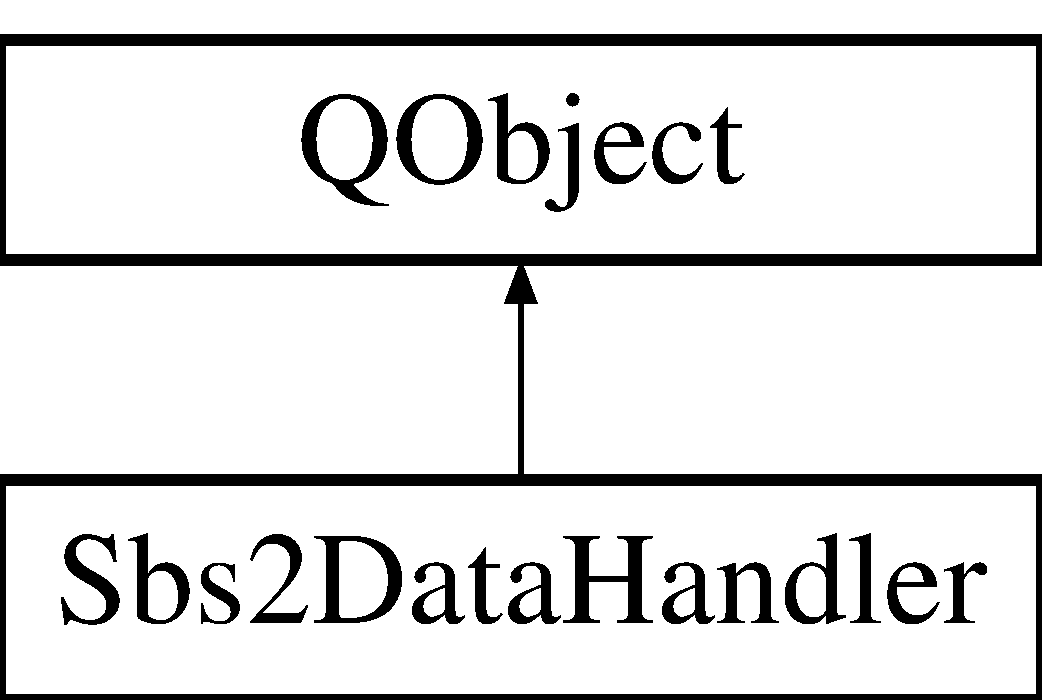
\includegraphics[height=2.000000cm]{classSbs2DataHandler}
\end{center}
\end{figure}
\subsection*{Public Slots}
\begin{DoxyCompactItemize}
\item 
void \hyperlink{classSbs2DataHandler_a0f7ac4379cc87dc4f84b764e810a2428}{set\-This\-Packet} (\hyperlink{classSbs2Packet}{Sbs2\-Packet} $\ast$this\-Packet\-\_\-)
\item 
void \hyperlink{classSbs2DataHandler_ae44b39aab30a6caa6768dfabad5d9e1b}{turn\-Filter\-On} (int fband\-Low\-\_\-, int fband\-High\-\_\-, int filter\-Order\-\_\-)
\item 
void \hyperlink{classSbs2DataHandler_a51df4501ee7314fe744acc098af30ee0}{turn\-Filter\-Off} ()
\item 
void \hyperlink{classSbs2DataHandler_ae45981d8b359448d850bb122376bbbb5}{start\-Recording} (Q\-String user, Q\-String description)
\item 
void \hyperlink{classSbs2DataHandler_a245b243ee7654d4e5bd506cd28a1d93b}{stop\-Recording} ()
\item 
void \hyperlink{classSbs2DataHandler_a79823cb73dcb66e0cf63d8892e906f75}{insert\-Into\-Meta\-File} (Q\-String event)
\item 
void \hyperlink{classSbs2DataHandler_ae4782ab78c11ceeda69a51cf7aec8c00}{turn\-Channel\-Spectrogram\-On} (int spectrogram\-Channel\-Samples\-\_\-=128, int spectrogram\-Channel\-Length\-\_\-=128, int spectrogram\-Channel\-Delta\-\_\-=0)
\item 
void \hyperlink{classSbs2DataHandler_ac949d6a7a1003dd908419369d1de4f22}{turn\-Channel\-Spectrogram\-Off} ()
\item 
void \hyperlink{classSbs2DataHandler_a0c6604942e87bf2690e8e6d48273559c}{set\-Window\-Type} (\hyperlink{classSbs2Spectrogram_a22265347883488b8385c83b67882d915}{Sbs2\-Spectrogram\-::\-Window\-Type} window\-Type)
\item 
void \hyperlink{classSbs2DataHandler_a2dfb1e3c5ad349c5a2c0f0271ab5d430}{set\-Source\-Reconstruction\-Vertices\-To\-Extract} (Q\-Vector$<$ int $>$ $\ast$vertices\-To\-Extract)
\item 
void \hyperlink{classSbs2DataHandler_a390b4440892561c1484e5c7a2ba6774b}{turn\-On\-Source\-Reconstruction\-Loreta} (int source\-Reconstruction\-Samples\-\_\-, int source\-Reconstruction\-Delta\-\_\-, int source\-Reconstruction\-Model\-Update\-Length\-\_\-, int source\-Reconstruction\-Model\-Update\-Delta\-\_\-, Q\-String hardware\-\_\-)
\item 
void \hyperlink{classSbs2DataHandler_a7ac252a2df8b1bc0d8fb70ee4b6fc257}{turn\-On\-Source\-Reconstruction\-Sparse} (int source\-Reconstruction\-Samples\-\_\-, Q\-Vector$<$ double $>$ lambdas, Q\-String hardware\-\_\-)
\item 
void \hyperlink{classSbs2DataHandler_ad9d1f6e27668fca2c7de888a35e1d76b}{do\-Source\-Reconstruction} ()
\begin{DoxyCompactList}\small\item\em Sbs2\-Data\-Handler\-::source\-Reconstruction. \end{DoxyCompactList}\item 
void \hyperlink{classSbs2DataHandler_aed81e6f317b7a8d13c50a56d2a3d25f9}{do\-Source\-Reconstruction\-Spectrogram} ()
\item 
void \hyperlink{classSbs2DataHandler_a0d89acf0f3db95346a7a1766cc5d9e53}{turn\-Off\-Source\-Reconstruction} ()
\item 
void \hyperlink{classSbs2DataHandler_a08378afb0dc485b61e6dd3d8df4725b7}{set\-Vertices\-To\-Extract} (Q\-Vector$<$ int $>$ $\ast$vertices\-To\-Extract)
\item 
void \hyperlink{classSbs2DataHandler_a204bf82c68e7d8a4200fa9b29550c853}{turn\-Send\-Raw\-Data\-On} (Q\-String raw\-Data\-Server\-Address\-\_\-, int raw\-Data\-Port\-\_\-, int raw\-Data\-Size\-\_\-=32, int raw\-Data\-Queue\-Length\-\_\-=8)
\item 
void \hyperlink{classSbs2DataHandler_a2d141bc0fd854ab32d67c5bdc9d44e05}{turn\-Send\-Raw\-Data\-Off} ()
\item 
void \hyperlink{classSbs2DataHandler_a3298d5245f738010bb9bfed5ca62c239}{add\-Raw\-Data\-Host} (Q\-String address, int port)
\item 
void \hyperlink{classSbs2DataHandler_ab19470d4bd133e153ca1e0096c29ce5f}{remove\-Raw\-Data\-Host} (Q\-String address, int port)
\item 
void \hyperlink{classSbs2DataHandler_a114c012077c938b091d572727ae0907c}{send\-Message} (Q\-String message, Q\-String address, int port)
\item 
void \hyperlink{classSbs2DataHandler_aaa0ebc6aaf9d93cf5f0774159efea37b}{send\-Message} (Q\-String message)
\item 
void \hyperlink{classSbs2DataHandler_a712a80f3cd44f014d80736ef9cf8c3ee}{add\-Message\-Udp\-Output\-Host} (Q\-String address, int port)
\item 
void \hyperlink{classSbs2DataHandler_aa7ce95acbe8b3868b9878e1ed7a8ba8f}{remove\-Message\-Udp\-Output\-Host} (Q\-String address)
\item 
void \hyperlink{classSbs2DataHandler_a0059ed6e559e1dead35d68e0daf43d33}{clear\-Message\-Udp\-Output\-Hosts} ()
\item 
void \hyperlink{classSbs2DataHandler_af5103e49754f879ffdc9cd137d67b69b}{turn\-Receive\-Message\-On} (Q\-String address, int port)
\item 
void \hyperlink{classSbs2DataHandler_a94414da810f2947f3868308818c14b1e}{turn\-Receive\-Message\-Off} ()
\item 
void \hyperlink{classSbs2DataHandler_addfa29ebc759d1fb5c2bf39f2fc5064c}{read\-Message} (Q\-String data, Q\-String sender, int sender\-Port)
\end{DoxyCompactItemize}
\subsection*{Signals}
\begin{DoxyCompactItemize}
\item 
void \hyperlink{classSbs2DataHandler_a6b044b68ab3c078889461095ae68b6a6}{spectrogram\-Updated} ()
\item 
void \hyperlink{classSbs2DataHandler_acfa19e08cc3317e782b945cd7d3adcbc}{source\-Reconstruction\-Ready} ()
\item 
void \hyperlink{classSbs2DataHandler_a5b443bf31daf7f1c235bf5503b11ee97}{source\-Reconstruction\-Spectrogram\-Ready} ()
\item 
void \hyperlink{classSbs2DataHandler_a1af8becf1c88098783238e1d4d9fa8f2}{set\-Window\-Type\-Signal} (\hyperlink{classSbs2Spectrogram_a22265347883488b8385c83b67882d915}{Sbs2\-Spectrogram\-::\-Window\-Type} window\-Type)
\item 
void \hyperlink{classSbs2DataHandler_a504ee9abc91fb5b7cec62c1eaedc6d92}{udp\-Message\-Received} (Q\-String data, Q\-String sender, int port)
\end{DoxyCompactItemize}
\subsection*{Public Member Functions}
\begin{DoxyCompactItemize}
\item 
\hyperlink{classSbs2DataHandler_a7ba4fb90e961ec8ff8958b271a6e746c}{Sbs2\-Data\-Handler} (Q\-Object $\ast$parent=0)
\item 
\hyperlink{classSbs2DataHandler_aaa08ce6949d3a979b9048fcdc280728e}{$\sim$\-Sbs2\-Data\-Handler} ()
\item 
virtual void \hyperlink{classSbs2DataHandler_adc6eccfe43b0759c5d4bc248b289e670}{filter} ()
\item 
virtual void \hyperlink{classSbs2DataHandler_a06ec994f323602e812cb548e6d78fddd}{record} ()
\item 
virtual Q\-String \hyperlink{classSbs2DataHandler_a4f429e3eab9329e386004e581eed5169}{get\-Raw\-Filename} ()
\item 
virtual void \hyperlink{classSbs2DataHandler_a97bb167202da122efccbce7566178645}{spectrogram\-Channel} ()
\item 
virtual void \hyperlink{classSbs2DataHandler_a523f8b5ffae2d11005196e4f7b39d1c5}{send\-Raw\-Data} ()
\item 
\hyperlink{classDTU_1_1DtuArray2D}{D\-T\-U\-::\-Dtu\-Array2\-D}$<$ double $>$ $\ast$ \hyperlink{classSbs2DataHandler_ace19ab4328535ed1929417d7079047ad}{get\-Power\-Values} ()
\item 
\hyperlink{classDTU_1_1DtuArray2D}{D\-T\-U\-::\-Dtu\-Array2\-D}$<$ double $>$ $\ast$ \hyperlink{classSbs2DataHandler_a3f9fda7e1bb37574752d79ff4507cfcd}{get\-Source\-Reconstruction\-Spectrogram\-Values} ()
\item 
\hyperlink{classDTU_1_1DtuArray2D}{D\-T\-U\-::\-Dtu\-Array2\-D}$<$ double $>$ $\ast$ \hyperlink{classSbs2DataHandler_a48501124932c256d9f2770b4fa50fc81}{get\-Source\-Reconstruction\-Mean\-Values} ()
\item 
int \hyperlink{classSbs2DataHandler_afd9db04705b6f39a7ee51db969929aaa}{get\-Packet\-Zero} ()
\end{DoxyCompactItemize}
\subsection*{Protected Member Functions}
\begin{DoxyCompactItemize}
\item 
virtual void \hyperlink{classSbs2DataHandler_a065dfd6e24bca97f2ca0958911b06f96}{reset} ()
\end{DoxyCompactItemize}
\subsection*{Protected Attributes}
\begin{DoxyCompactItemize}
\item 
int \hyperlink{classSbs2DataHandler_a283d44a7f76c0943073e4b1e1f3a47e0}{samples\-Collected}
\item 
\hyperlink{classSbs2Packet}{Sbs2\-Packet} $\ast$ \hyperlink{classSbs2DataHandler_a7978367be1b4e77d29bd070749f9b90b}{this\-Packet}
\item 
int \hyperlink{classSbs2DataHandler_ac98441bbba779fc5d545b91fff4fe4af}{filter\-On}
\item 
int \hyperlink{classSbs2DataHandler_a3950a87e3197897c454f36a6e0cbe0c2}{filter\-Order}
\item 
int \hyperlink{classSbs2DataHandler_aa151649a496b0c6fb4fff0504de0cb84}{fband\-Low}
\item 
int \hyperlink{classSbs2DataHandler_a97a3294b785f95342192060884b7a51f}{fband\-High}
\item 
\hyperlink{classSbs2Filter}{Sbs2\-Filter} $\ast$ \hyperlink{classSbs2DataHandler_ab4ff2034bf7974feac4655767ffb2f06}{sbs2\-Filter}
\item 
\hyperlink{classDTU_1_1DtuArray2D}{D\-T\-U\-::\-Dtu\-Array2\-D}$<$ double $>$ $\ast$ \hyperlink{classSbs2DataHandler_a945b3c5c16c586b7ea7c3fa2a61f1314}{to\-Filter\-Values}
\item 
\hyperlink{classDTU_1_1DtuArray2D}{D\-T\-U\-::\-Dtu\-Array2\-D}$<$ double $>$ $\ast$ \hyperlink{classSbs2DataHandler_ab59d6276b75e1b28c622cfd013c8cf8d}{filter\-Result\-Values}
\item 
int \hyperlink{classSbs2DataHandler_ae6505076adb777fb2786f5cf1cc4caa5}{recording}
\item 
\hyperlink{classSbs2FileHandler}{Sbs2\-File\-Handler} $\ast$ \hyperlink{classSbs2DataHandler_a21a05a8191f99d973e03949016cc6362}{sbs2\-File\-Handler}
\item 
int \hyperlink{classSbs2DataHandler_a6aec777856b21566fc7c1c239bc01a6e}{spectrogram\-Channel\-On}
\item 
int \hyperlink{classSbs2DataHandler_ae19dc07959f3dfedbdd020c8ecaa1b20}{spectrogram\-Channel\-Samples}
\item 
int \hyperlink{classSbs2DataHandler_aac9d4579ad6b4d84e205ccf834bccf79}{spectrogram\-Channel\-Length}
\item 
int \hyperlink{classSbs2DataHandler_a2ca4e80598926e06fb224c985a0000f1}{spectrogram\-Channel\-Delta}
\item 
int \hyperlink{classSbs2DataHandler_a5f13f58b4c6fc3ef242c49526f632fb5}{spectrogram\-Channel\-Delta\-Collected}
\item 
\hyperlink{classSbs2Spectrogram}{Sbs2\-Spectrogram} $\ast$ \hyperlink{classSbs2DataHandler_a8f10be73e5dcf79ee2b17dc25b8c3ad3}{sbs2\-Spectrogram}
\item 
\hyperlink{classDTU_1_1DtuArray2D}{D\-T\-U\-::\-Dtu\-Array2\-D}$<$ double $>$ $\ast$ \hyperlink{classSbs2DataHandler_a2e2a930ac63df2480e02bfc2cc2d9c56}{to\-Spectrogram\-Values}
\item 
\hyperlink{classDTU_1_1DtuArray2D}{D\-T\-U\-::\-Dtu\-Array2\-D}$<$ double $>$ $\ast$ \hyperlink{classSbs2DataHandler_a71fb5afb898d4998d271c6812d3b13bc}{spectrogram\-Values}
\item 
\hyperlink{classDTU_1_1DtuArray2D}{D\-T\-U\-::\-Dtu\-Array2\-D}$<$ double $>$ $\ast$ \hyperlink{classSbs2DataHandler_a2e654257d666ee18603aa21ce4fc0094}{power\-Values}
\item 
Q\-String \hyperlink{classSbs2DataHandler_a7707e1c381de4da234da0e1a427ea943}{source\-Reconstruction\-Method}
\item 
int \hyperlink{classSbs2DataHandler_ac39dd9d7e16c5483c9c8264ab9fe3583}{source\-Reconstruction\-On}
\item 
int \hyperlink{classSbs2DataHandler_a27824cd8b891d39371317f6b71734bb9}{is\-Source\-Reconstruction\-Ready}
\item 
int \hyperlink{classSbs2DataHandler_a040c1f1987d1aedd9fc4fa0bb032793c}{source\-Reconstruction\-Samples}
\item 
int \hyperlink{classSbs2DataHandler_a518bfd8fdb83c367de2aad22d941e237}{source\-Reconstruction\-Delta}
\item 
int \hyperlink{classSbs2DataHandler_a9252e8ca95c93cf6040872fc63e5be2a}{source\-Reconstruction\-Delta\-Collected}
\item 
int \hyperlink{classSbs2DataHandler_a8fd8e83392c3e765248a1159ea7ab4f0}{source\-Reconstruction\-Model\-Update\-Length}
\item 
int \hyperlink{classSbs2DataHandler_ab73812b83ec8bf91093d35c706a524bc}{source\-Reconstruction\-Model\-Update\-Delta}
\item 
int \hyperlink{classSbs2DataHandler_a00267a9a5aeb1d0cc19c10d35bb74244}{ready\-To\-Reconstruct}
\item 
Q\-String \hyperlink{classSbs2DataHandler_a2aefd1effca8fce9a50d996a8904d3db}{hardware}
\item 
\hyperlink{classSbs2SourceReconstruction}{Sbs2\-Source\-Reconstruction} $\ast$ \hyperlink{classSbs2DataHandler_a0f5dcab81112672a955fe3571b27b257}{sbs2\-Source\-Reconstruction}
\item 
\hyperlink{classDTU_1_1DtuArray2D}{D\-T\-U\-::\-Dtu\-Array2\-D}$<$ double $>$ $\ast$ \hyperlink{classSbs2DataHandler_a85ec29b438414d29f31b7c2d894155db}{to\-Source\-Reconstruction\-Values}
\item 
\hyperlink{classDTU_1_1DtuArray2D}{D\-T\-U\-::\-Dtu\-Array2\-D}$<$ double $>$ $\ast$ \hyperlink{classSbs2DataHandler_a74adbe08c28c63df93c29f7ceeaac938}{source\-Reconstruction\-Values}
\item 
\hyperlink{classDTU_1_1DtuArray2D}{D\-T\-U\-::\-Dtu\-Array2\-D}$<$ double $>$ $\ast$ \hyperlink{classSbs2DataHandler_abb128e26db79c4bf6c6064b3714a9205}{source\-Reconstruction\-Spectrogram\-Values}
\item 
int \hyperlink{classSbs2DataHandler_adc249819610b0d1fe352e882d842c36a}{network\-Send\-Raw\-Data\-On}
\item 
\hyperlink{classSbs2NetworkHandler}{Sbs2\-Network\-Handler} $\ast$ \hyperlink{classSbs2DataHandler_a5bc26d06be4b58f25ec0b88b27773fb0}{sbs2\-Network\-Handler}
\item 
int \hyperlink{classSbs2DataHandler_a9f67857de7323c19164523e6f2296915}{packets\-Seen}
\end{DoxyCompactItemize}


\subsection{Constructor \& Destructor Documentation}
\hypertarget{classSbs2DataHandler_a7ba4fb90e961ec8ff8958b271a6e746c}{\index{Sbs2\-Data\-Handler@{Sbs2\-Data\-Handler}!Sbs2\-Data\-Handler@{Sbs2\-Data\-Handler}}
\index{Sbs2\-Data\-Handler@{Sbs2\-Data\-Handler}!Sbs2DataHandler@{Sbs2\-Data\-Handler}}
\subsubsection[{Sbs2\-Data\-Handler}]{\setlength{\rightskip}{0pt plus 5cm}Sbs2\-Data\-Handler\-::\-Sbs2\-Data\-Handler (
\begin{DoxyParamCaption}
\item[{Q\-Object $\ast$}]{parent = {\ttfamily 0}}
\end{DoxyParamCaption}
)\hspace{0.3cm}{\ttfamily [explicit]}}}\label{classSbs2DataHandler_a7ba4fb90e961ec8ff8958b271a6e746c}
\hypertarget{classSbs2DataHandler_aaa08ce6949d3a979b9048fcdc280728e}{\index{Sbs2\-Data\-Handler@{Sbs2\-Data\-Handler}!$\sim$\-Sbs2\-Data\-Handler@{$\sim$\-Sbs2\-Data\-Handler}}
\index{$\sim$\-Sbs2\-Data\-Handler@{$\sim$\-Sbs2\-Data\-Handler}!Sbs2DataHandler@{Sbs2\-Data\-Handler}}
\subsubsection[{$\sim$\-Sbs2\-Data\-Handler}]{\setlength{\rightskip}{0pt plus 5cm}Sbs2\-Data\-Handler\-::$\sim$\-Sbs2\-Data\-Handler (
\begin{DoxyParamCaption}
{}
\end{DoxyParamCaption}
)}}\label{classSbs2DataHandler_aaa08ce6949d3a979b9048fcdc280728e}


\subsection{Member Function Documentation}
\hypertarget{classSbs2DataHandler_a712a80f3cd44f014d80736ef9cf8c3ee}{\index{Sbs2\-Data\-Handler@{Sbs2\-Data\-Handler}!add\-Message\-Udp\-Output\-Host@{add\-Message\-Udp\-Output\-Host}}
\index{add\-Message\-Udp\-Output\-Host@{add\-Message\-Udp\-Output\-Host}!Sbs2DataHandler@{Sbs2\-Data\-Handler}}
\subsubsection[{add\-Message\-Udp\-Output\-Host}]{\setlength{\rightskip}{0pt plus 5cm}void Sbs2\-Data\-Handler\-::add\-Message\-Udp\-Output\-Host (
\begin{DoxyParamCaption}
\item[{Q\-String}]{address, }
\item[{int}]{port}
\end{DoxyParamCaption}
)\hspace{0.3cm}{\ttfamily [slot]}}}\label{classSbs2DataHandler_a712a80f3cd44f014d80736ef9cf8c3ee}
\hypertarget{classSbs2DataHandler_a3298d5245f738010bb9bfed5ca62c239}{\index{Sbs2\-Data\-Handler@{Sbs2\-Data\-Handler}!add\-Raw\-Data\-Host@{add\-Raw\-Data\-Host}}
\index{add\-Raw\-Data\-Host@{add\-Raw\-Data\-Host}!Sbs2DataHandler@{Sbs2\-Data\-Handler}}
\subsubsection[{add\-Raw\-Data\-Host}]{\setlength{\rightskip}{0pt plus 5cm}void Sbs2\-Data\-Handler\-::add\-Raw\-Data\-Host (
\begin{DoxyParamCaption}
\item[{Q\-String}]{address, }
\item[{int}]{port}
\end{DoxyParamCaption}
)\hspace{0.3cm}{\ttfamily [slot]}}}\label{classSbs2DataHandler_a3298d5245f738010bb9bfed5ca62c239}
\hypertarget{classSbs2DataHandler_a0059ed6e559e1dead35d68e0daf43d33}{\index{Sbs2\-Data\-Handler@{Sbs2\-Data\-Handler}!clear\-Message\-Udp\-Output\-Hosts@{clear\-Message\-Udp\-Output\-Hosts}}
\index{clear\-Message\-Udp\-Output\-Hosts@{clear\-Message\-Udp\-Output\-Hosts}!Sbs2DataHandler@{Sbs2\-Data\-Handler}}
\subsubsection[{clear\-Message\-Udp\-Output\-Hosts}]{\setlength{\rightskip}{0pt plus 5cm}void Sbs2\-Data\-Handler\-::clear\-Message\-Udp\-Output\-Hosts (
\begin{DoxyParamCaption}
{}
\end{DoxyParamCaption}
)\hspace{0.3cm}{\ttfamily [slot]}}}\label{classSbs2DataHandler_a0059ed6e559e1dead35d68e0daf43d33}
\hypertarget{classSbs2DataHandler_ad9d1f6e27668fca2c7de888a35e1d76b}{\index{Sbs2\-Data\-Handler@{Sbs2\-Data\-Handler}!do\-Source\-Reconstruction@{do\-Source\-Reconstruction}}
\index{do\-Source\-Reconstruction@{do\-Source\-Reconstruction}!Sbs2DataHandler@{Sbs2\-Data\-Handler}}
\subsubsection[{do\-Source\-Reconstruction}]{\setlength{\rightskip}{0pt plus 5cm}void Sbs2\-Data\-Handler\-::do\-Source\-Reconstruction (
\begin{DoxyParamCaption}
{}
\end{DoxyParamCaption}
)\hspace{0.3cm}{\ttfamily [slot]}}}\label{classSbs2DataHandler_ad9d1f6e27668fca2c7de888a35e1d76b}


Sbs2\-Data\-Handler\-::source\-Reconstruction. 

Runs the source reconstruction with Sbs2\-Source\-Reconstrucion\-::do\-Rec. This only happes is 'source\-Reconstruction\-On' is turned on. This variable is controlled by Sbs2\-Data\-Handler\-::turn\-Source\-Reconstruction\-On \hypertarget{classSbs2DataHandler_aed81e6f317b7a8d13c50a56d2a3d25f9}{\index{Sbs2\-Data\-Handler@{Sbs2\-Data\-Handler}!do\-Source\-Reconstruction\-Spectrogram@{do\-Source\-Reconstruction\-Spectrogram}}
\index{do\-Source\-Reconstruction\-Spectrogram@{do\-Source\-Reconstruction\-Spectrogram}!Sbs2DataHandler@{Sbs2\-Data\-Handler}}
\subsubsection[{do\-Source\-Reconstruction\-Spectrogram}]{\setlength{\rightskip}{0pt plus 5cm}void Sbs2\-Data\-Handler\-::do\-Source\-Reconstruction\-Spectrogram (
\begin{DoxyParamCaption}
{}
\end{DoxyParamCaption}
)\hspace{0.3cm}{\ttfamily [slot]}}}\label{classSbs2DataHandler_aed81e6f317b7a8d13c50a56d2a3d25f9}
\hypertarget{classSbs2DataHandler_adc6eccfe43b0759c5d4bc248b289e670}{\index{Sbs2\-Data\-Handler@{Sbs2\-Data\-Handler}!filter@{filter}}
\index{filter@{filter}!Sbs2DataHandler@{Sbs2\-Data\-Handler}}
\subsubsection[{filter}]{\setlength{\rightskip}{0pt plus 5cm}void Sbs2\-Data\-Handler\-::filter (
\begin{DoxyParamCaption}
{}
\end{DoxyParamCaption}
)\hspace{0.3cm}{\ttfamily [virtual]}}}\label{classSbs2DataHandler_adc6eccfe43b0759c5d4bc248b289e670}
\hypertarget{classSbs2DataHandler_afd9db04705b6f39a7ee51db969929aaa}{\index{Sbs2\-Data\-Handler@{Sbs2\-Data\-Handler}!get\-Packet\-Zero@{get\-Packet\-Zero}}
\index{get\-Packet\-Zero@{get\-Packet\-Zero}!Sbs2DataHandler@{Sbs2\-Data\-Handler}}
\subsubsection[{get\-Packet\-Zero}]{\setlength{\rightskip}{0pt plus 5cm}int Sbs2\-Data\-Handler\-::get\-Packet\-Zero (
\begin{DoxyParamCaption}
{}
\end{DoxyParamCaption}
)}}\label{classSbs2DataHandler_afd9db04705b6f39a7ee51db969929aaa}
\hypertarget{classSbs2DataHandler_ace19ab4328535ed1929417d7079047ad}{\index{Sbs2\-Data\-Handler@{Sbs2\-Data\-Handler}!get\-Power\-Values@{get\-Power\-Values}}
\index{get\-Power\-Values@{get\-Power\-Values}!Sbs2DataHandler@{Sbs2\-Data\-Handler}}
\subsubsection[{get\-Power\-Values}]{\setlength{\rightskip}{0pt plus 5cm}{\bf D\-T\-U\-::\-Dtu\-Array2\-D}$<$ double $>$ $\ast$ Sbs2\-Data\-Handler\-::get\-Power\-Values (
\begin{DoxyParamCaption}
{}
\end{DoxyParamCaption}
)}}\label{classSbs2DataHandler_ace19ab4328535ed1929417d7079047ad}
\hypertarget{classSbs2DataHandler_a4f429e3eab9329e386004e581eed5169}{\index{Sbs2\-Data\-Handler@{Sbs2\-Data\-Handler}!get\-Raw\-Filename@{get\-Raw\-Filename}}
\index{get\-Raw\-Filename@{get\-Raw\-Filename}!Sbs2DataHandler@{Sbs2\-Data\-Handler}}
\subsubsection[{get\-Raw\-Filename}]{\setlength{\rightskip}{0pt plus 5cm}Q\-String Sbs2\-Data\-Handler\-::get\-Raw\-Filename (
\begin{DoxyParamCaption}
{}
\end{DoxyParamCaption}
)\hspace{0.3cm}{\ttfamily [virtual]}}}\label{classSbs2DataHandler_a4f429e3eab9329e386004e581eed5169}
\hypertarget{classSbs2DataHandler_a48501124932c256d9f2770b4fa50fc81}{\index{Sbs2\-Data\-Handler@{Sbs2\-Data\-Handler}!get\-Source\-Reconstruction\-Mean\-Values@{get\-Source\-Reconstruction\-Mean\-Values}}
\index{get\-Source\-Reconstruction\-Mean\-Values@{get\-Source\-Reconstruction\-Mean\-Values}!Sbs2DataHandler@{Sbs2\-Data\-Handler}}
\subsubsection[{get\-Source\-Reconstruction\-Mean\-Values}]{\setlength{\rightskip}{0pt plus 5cm}{\bf D\-T\-U\-::\-Dtu\-Array2\-D}$<$ double $>$ $\ast$ Sbs2\-Data\-Handler\-::get\-Source\-Reconstruction\-Mean\-Values (
\begin{DoxyParamCaption}
{}
\end{DoxyParamCaption}
)}}\label{classSbs2DataHandler_a48501124932c256d9f2770b4fa50fc81}
\hypertarget{classSbs2DataHandler_a3f9fda7e1bb37574752d79ff4507cfcd}{\index{Sbs2\-Data\-Handler@{Sbs2\-Data\-Handler}!get\-Source\-Reconstruction\-Spectrogram\-Values@{get\-Source\-Reconstruction\-Spectrogram\-Values}}
\index{get\-Source\-Reconstruction\-Spectrogram\-Values@{get\-Source\-Reconstruction\-Spectrogram\-Values}!Sbs2DataHandler@{Sbs2\-Data\-Handler}}
\subsubsection[{get\-Source\-Reconstruction\-Spectrogram\-Values}]{\setlength{\rightskip}{0pt plus 5cm}{\bf D\-T\-U\-::\-Dtu\-Array2\-D}$<$ double $>$ $\ast$ Sbs2\-Data\-Handler\-::get\-Source\-Reconstruction\-Spectrogram\-Values (
\begin{DoxyParamCaption}
{}
\end{DoxyParamCaption}
)}}\label{classSbs2DataHandler_a3f9fda7e1bb37574752d79ff4507cfcd}
\hypertarget{classSbs2DataHandler_a79823cb73dcb66e0cf63d8892e906f75}{\index{Sbs2\-Data\-Handler@{Sbs2\-Data\-Handler}!insert\-Into\-Meta\-File@{insert\-Into\-Meta\-File}}
\index{insert\-Into\-Meta\-File@{insert\-Into\-Meta\-File}!Sbs2DataHandler@{Sbs2\-Data\-Handler}}
\subsubsection[{insert\-Into\-Meta\-File}]{\setlength{\rightskip}{0pt plus 5cm}void Sbs2\-Data\-Handler\-::insert\-Into\-Meta\-File (
\begin{DoxyParamCaption}
\item[{Q\-String}]{event}
\end{DoxyParamCaption}
)\hspace{0.3cm}{\ttfamily [slot]}}}\label{classSbs2DataHandler_a79823cb73dcb66e0cf63d8892e906f75}
\hypertarget{classSbs2DataHandler_addfa29ebc759d1fb5c2bf39f2fc5064c}{\index{Sbs2\-Data\-Handler@{Sbs2\-Data\-Handler}!read\-Message@{read\-Message}}
\index{read\-Message@{read\-Message}!Sbs2DataHandler@{Sbs2\-Data\-Handler}}
\subsubsection[{read\-Message}]{\setlength{\rightskip}{0pt plus 5cm}void Sbs2\-Data\-Handler\-::read\-Message (
\begin{DoxyParamCaption}
\item[{Q\-String}]{data, }
\item[{Q\-String}]{sender, }
\item[{int}]{sender\-Port}
\end{DoxyParamCaption}
)\hspace{0.3cm}{\ttfamily [slot]}}}\label{classSbs2DataHandler_addfa29ebc759d1fb5c2bf39f2fc5064c}
\hypertarget{classSbs2DataHandler_a06ec994f323602e812cb548e6d78fddd}{\index{Sbs2\-Data\-Handler@{Sbs2\-Data\-Handler}!record@{record}}
\index{record@{record}!Sbs2DataHandler@{Sbs2\-Data\-Handler}}
\subsubsection[{record}]{\setlength{\rightskip}{0pt plus 5cm}void Sbs2\-Data\-Handler\-::record (
\begin{DoxyParamCaption}
{}
\end{DoxyParamCaption}
)\hspace{0.3cm}{\ttfamily [virtual]}}}\label{classSbs2DataHandler_a06ec994f323602e812cb548e6d78fddd}
\hypertarget{classSbs2DataHandler_aa7ce95acbe8b3868b9878e1ed7a8ba8f}{\index{Sbs2\-Data\-Handler@{Sbs2\-Data\-Handler}!remove\-Message\-Udp\-Output\-Host@{remove\-Message\-Udp\-Output\-Host}}
\index{remove\-Message\-Udp\-Output\-Host@{remove\-Message\-Udp\-Output\-Host}!Sbs2DataHandler@{Sbs2\-Data\-Handler}}
\subsubsection[{remove\-Message\-Udp\-Output\-Host}]{\setlength{\rightskip}{0pt plus 5cm}void Sbs2\-Data\-Handler\-::remove\-Message\-Udp\-Output\-Host (
\begin{DoxyParamCaption}
\item[{Q\-String}]{address}
\end{DoxyParamCaption}
)\hspace{0.3cm}{\ttfamily [slot]}}}\label{classSbs2DataHandler_aa7ce95acbe8b3868b9878e1ed7a8ba8f}
\hypertarget{classSbs2DataHandler_ab19470d4bd133e153ca1e0096c29ce5f}{\index{Sbs2\-Data\-Handler@{Sbs2\-Data\-Handler}!remove\-Raw\-Data\-Host@{remove\-Raw\-Data\-Host}}
\index{remove\-Raw\-Data\-Host@{remove\-Raw\-Data\-Host}!Sbs2DataHandler@{Sbs2\-Data\-Handler}}
\subsubsection[{remove\-Raw\-Data\-Host}]{\setlength{\rightskip}{0pt plus 5cm}void Sbs2\-Data\-Handler\-::remove\-Raw\-Data\-Host (
\begin{DoxyParamCaption}
\item[{Q\-String}]{address, }
\item[{int}]{port}
\end{DoxyParamCaption}
)\hspace{0.3cm}{\ttfamily [slot]}}}\label{classSbs2DataHandler_ab19470d4bd133e153ca1e0096c29ce5f}
\hypertarget{classSbs2DataHandler_a065dfd6e24bca97f2ca0958911b06f96}{\index{Sbs2\-Data\-Handler@{Sbs2\-Data\-Handler}!reset@{reset}}
\index{reset@{reset}!Sbs2DataHandler@{Sbs2\-Data\-Handler}}
\subsubsection[{reset}]{\setlength{\rightskip}{0pt plus 5cm}void Sbs2\-Data\-Handler\-::reset (
\begin{DoxyParamCaption}
{}
\end{DoxyParamCaption}
)\hspace{0.3cm}{\ttfamily [protected]}, {\ttfamily [virtual]}}}\label{classSbs2DataHandler_a065dfd6e24bca97f2ca0958911b06f96}
\hypertarget{classSbs2DataHandler_a114c012077c938b091d572727ae0907c}{\index{Sbs2\-Data\-Handler@{Sbs2\-Data\-Handler}!send\-Message@{send\-Message}}
\index{send\-Message@{send\-Message}!Sbs2DataHandler@{Sbs2\-Data\-Handler}}
\subsubsection[{send\-Message}]{\setlength{\rightskip}{0pt plus 5cm}void Sbs2\-Data\-Handler\-::send\-Message (
\begin{DoxyParamCaption}
\item[{Q\-String}]{message, }
\item[{Q\-String}]{address, }
\item[{int}]{port}
\end{DoxyParamCaption}
)\hspace{0.3cm}{\ttfamily [slot]}}}\label{classSbs2DataHandler_a114c012077c938b091d572727ae0907c}
\hypertarget{classSbs2DataHandler_aaa0ebc6aaf9d93cf5f0774159efea37b}{\index{Sbs2\-Data\-Handler@{Sbs2\-Data\-Handler}!send\-Message@{send\-Message}}
\index{send\-Message@{send\-Message}!Sbs2DataHandler@{Sbs2\-Data\-Handler}}
\subsubsection[{send\-Message}]{\setlength{\rightskip}{0pt plus 5cm}void Sbs2\-Data\-Handler\-::send\-Message (
\begin{DoxyParamCaption}
\item[{Q\-String}]{message}
\end{DoxyParamCaption}
)\hspace{0.3cm}{\ttfamily [slot]}}}\label{classSbs2DataHandler_aaa0ebc6aaf9d93cf5f0774159efea37b}
\hypertarget{classSbs2DataHandler_a523f8b5ffae2d11005196e4f7b39d1c5}{\index{Sbs2\-Data\-Handler@{Sbs2\-Data\-Handler}!send\-Raw\-Data@{send\-Raw\-Data}}
\index{send\-Raw\-Data@{send\-Raw\-Data}!Sbs2DataHandler@{Sbs2\-Data\-Handler}}
\subsubsection[{send\-Raw\-Data}]{\setlength{\rightskip}{0pt plus 5cm}void Sbs2\-Data\-Handler\-::send\-Raw\-Data (
\begin{DoxyParamCaption}
{}
\end{DoxyParamCaption}
)\hspace{0.3cm}{\ttfamily [virtual]}}}\label{classSbs2DataHandler_a523f8b5ffae2d11005196e4f7b39d1c5}
\hypertarget{classSbs2DataHandler_a2dfb1e3c5ad349c5a2c0f0271ab5d430}{\index{Sbs2\-Data\-Handler@{Sbs2\-Data\-Handler}!set\-Source\-Reconstruction\-Vertices\-To\-Extract@{set\-Source\-Reconstruction\-Vertices\-To\-Extract}}
\index{set\-Source\-Reconstruction\-Vertices\-To\-Extract@{set\-Source\-Reconstruction\-Vertices\-To\-Extract}!Sbs2DataHandler@{Sbs2\-Data\-Handler}}
\subsubsection[{set\-Source\-Reconstruction\-Vertices\-To\-Extract}]{\setlength{\rightskip}{0pt plus 5cm}void Sbs2\-Data\-Handler\-::set\-Source\-Reconstruction\-Vertices\-To\-Extract (
\begin{DoxyParamCaption}
\item[{Q\-Vector$<$ int $>$ $\ast$}]{vertices\-To\-Extract}
\end{DoxyParamCaption}
)\hspace{0.3cm}{\ttfamily [slot]}}}\label{classSbs2DataHandler_a2dfb1e3c5ad349c5a2c0f0271ab5d430}
\hypertarget{classSbs2DataHandler_a0f7ac4379cc87dc4f84b764e810a2428}{\index{Sbs2\-Data\-Handler@{Sbs2\-Data\-Handler}!set\-This\-Packet@{set\-This\-Packet}}
\index{set\-This\-Packet@{set\-This\-Packet}!Sbs2DataHandler@{Sbs2\-Data\-Handler}}
\subsubsection[{set\-This\-Packet}]{\setlength{\rightskip}{0pt plus 5cm}void Sbs2\-Data\-Handler\-::set\-This\-Packet (
\begin{DoxyParamCaption}
\item[{{\bf Sbs2\-Packet} $\ast$}]{this\-Packet\-\_\-}
\end{DoxyParamCaption}
)\hspace{0.3cm}{\ttfamily [slot]}}}\label{classSbs2DataHandler_a0f7ac4379cc87dc4f84b764e810a2428}
\hypertarget{classSbs2DataHandler_a08378afb0dc485b61e6dd3d8df4725b7}{\index{Sbs2\-Data\-Handler@{Sbs2\-Data\-Handler}!set\-Vertices\-To\-Extract@{set\-Vertices\-To\-Extract}}
\index{set\-Vertices\-To\-Extract@{set\-Vertices\-To\-Extract}!Sbs2DataHandler@{Sbs2\-Data\-Handler}}
\subsubsection[{set\-Vertices\-To\-Extract}]{\setlength{\rightskip}{0pt plus 5cm}void Sbs2\-Data\-Handler\-::set\-Vertices\-To\-Extract (
\begin{DoxyParamCaption}
\item[{Q\-Vector$<$ int $>$ $\ast$}]{vertices\-To\-Extract}
\end{DoxyParamCaption}
)\hspace{0.3cm}{\ttfamily [slot]}}}\label{classSbs2DataHandler_a08378afb0dc485b61e6dd3d8df4725b7}
\hypertarget{classSbs2DataHandler_a0c6604942e87bf2690e8e6d48273559c}{\index{Sbs2\-Data\-Handler@{Sbs2\-Data\-Handler}!set\-Window\-Type@{set\-Window\-Type}}
\index{set\-Window\-Type@{set\-Window\-Type}!Sbs2DataHandler@{Sbs2\-Data\-Handler}}
\subsubsection[{set\-Window\-Type}]{\setlength{\rightskip}{0pt plus 5cm}void Sbs2\-Data\-Handler\-::set\-Window\-Type (
\begin{DoxyParamCaption}
\item[{{\bf Sbs2\-Spectrogram\-::\-Window\-Type}}]{window\-Type}
\end{DoxyParamCaption}
)\hspace{0.3cm}{\ttfamily [slot]}}}\label{classSbs2DataHandler_a0c6604942e87bf2690e8e6d48273559c}
\hypertarget{classSbs2DataHandler_a1af8becf1c88098783238e1d4d9fa8f2}{\index{Sbs2\-Data\-Handler@{Sbs2\-Data\-Handler}!set\-Window\-Type\-Signal@{set\-Window\-Type\-Signal}}
\index{set\-Window\-Type\-Signal@{set\-Window\-Type\-Signal}!Sbs2DataHandler@{Sbs2\-Data\-Handler}}
\subsubsection[{set\-Window\-Type\-Signal}]{\setlength{\rightskip}{0pt plus 5cm}void Sbs2\-Data\-Handler\-::set\-Window\-Type\-Signal (
\begin{DoxyParamCaption}
\item[{{\bf Sbs2\-Spectrogram\-::\-Window\-Type}}]{window\-Type}
\end{DoxyParamCaption}
)\hspace{0.3cm}{\ttfamily [signal]}}}\label{classSbs2DataHandler_a1af8becf1c88098783238e1d4d9fa8f2}
\hypertarget{classSbs2DataHandler_acfa19e08cc3317e782b945cd7d3adcbc}{\index{Sbs2\-Data\-Handler@{Sbs2\-Data\-Handler}!source\-Reconstruction\-Ready@{source\-Reconstruction\-Ready}}
\index{source\-Reconstruction\-Ready@{source\-Reconstruction\-Ready}!Sbs2DataHandler@{Sbs2\-Data\-Handler}}
\subsubsection[{source\-Reconstruction\-Ready}]{\setlength{\rightskip}{0pt plus 5cm}void Sbs2\-Data\-Handler\-::source\-Reconstruction\-Ready (
\begin{DoxyParamCaption}
{}
\end{DoxyParamCaption}
)\hspace{0.3cm}{\ttfamily [signal]}}}\label{classSbs2DataHandler_acfa19e08cc3317e782b945cd7d3adcbc}
\hypertarget{classSbs2DataHandler_a5b443bf31daf7f1c235bf5503b11ee97}{\index{Sbs2\-Data\-Handler@{Sbs2\-Data\-Handler}!source\-Reconstruction\-Spectrogram\-Ready@{source\-Reconstruction\-Spectrogram\-Ready}}
\index{source\-Reconstruction\-Spectrogram\-Ready@{source\-Reconstruction\-Spectrogram\-Ready}!Sbs2DataHandler@{Sbs2\-Data\-Handler}}
\subsubsection[{source\-Reconstruction\-Spectrogram\-Ready}]{\setlength{\rightskip}{0pt plus 5cm}void Sbs2\-Data\-Handler\-::source\-Reconstruction\-Spectrogram\-Ready (
\begin{DoxyParamCaption}
{}
\end{DoxyParamCaption}
)\hspace{0.3cm}{\ttfamily [signal]}}}\label{classSbs2DataHandler_a5b443bf31daf7f1c235bf5503b11ee97}
\hypertarget{classSbs2DataHandler_a97bb167202da122efccbce7566178645}{\index{Sbs2\-Data\-Handler@{Sbs2\-Data\-Handler}!spectrogram\-Channel@{spectrogram\-Channel}}
\index{spectrogram\-Channel@{spectrogram\-Channel}!Sbs2DataHandler@{Sbs2\-Data\-Handler}}
\subsubsection[{spectrogram\-Channel}]{\setlength{\rightskip}{0pt plus 5cm}void Sbs2\-Data\-Handler\-::spectrogram\-Channel (
\begin{DoxyParamCaption}
{}
\end{DoxyParamCaption}
)\hspace{0.3cm}{\ttfamily [virtual]}}}\label{classSbs2DataHandler_a97bb167202da122efccbce7566178645}
\hypertarget{classSbs2DataHandler_a6b044b68ab3c078889461095ae68b6a6}{\index{Sbs2\-Data\-Handler@{Sbs2\-Data\-Handler}!spectrogram\-Updated@{spectrogram\-Updated}}
\index{spectrogram\-Updated@{spectrogram\-Updated}!Sbs2DataHandler@{Sbs2\-Data\-Handler}}
\subsubsection[{spectrogram\-Updated}]{\setlength{\rightskip}{0pt plus 5cm}void Sbs2\-Data\-Handler\-::spectrogram\-Updated (
\begin{DoxyParamCaption}
{}
\end{DoxyParamCaption}
)\hspace{0.3cm}{\ttfamily [signal]}}}\label{classSbs2DataHandler_a6b044b68ab3c078889461095ae68b6a6}
\hypertarget{classSbs2DataHandler_ae45981d8b359448d850bb122376bbbb5}{\index{Sbs2\-Data\-Handler@{Sbs2\-Data\-Handler}!start\-Recording@{start\-Recording}}
\index{start\-Recording@{start\-Recording}!Sbs2DataHandler@{Sbs2\-Data\-Handler}}
\subsubsection[{start\-Recording}]{\setlength{\rightskip}{0pt plus 5cm}void Sbs2\-Data\-Handler\-::start\-Recording (
\begin{DoxyParamCaption}
\item[{Q\-String}]{user, }
\item[{Q\-String}]{description}
\end{DoxyParamCaption}
)\hspace{0.3cm}{\ttfamily [slot]}}}\label{classSbs2DataHandler_ae45981d8b359448d850bb122376bbbb5}
\hypertarget{classSbs2DataHandler_a245b243ee7654d4e5bd506cd28a1d93b}{\index{Sbs2\-Data\-Handler@{Sbs2\-Data\-Handler}!stop\-Recording@{stop\-Recording}}
\index{stop\-Recording@{stop\-Recording}!Sbs2DataHandler@{Sbs2\-Data\-Handler}}
\subsubsection[{stop\-Recording}]{\setlength{\rightskip}{0pt plus 5cm}void Sbs2\-Data\-Handler\-::stop\-Recording (
\begin{DoxyParamCaption}
{}
\end{DoxyParamCaption}
)\hspace{0.3cm}{\ttfamily [slot]}}}\label{classSbs2DataHandler_a245b243ee7654d4e5bd506cd28a1d93b}
\hypertarget{classSbs2DataHandler_ac949d6a7a1003dd908419369d1de4f22}{\index{Sbs2\-Data\-Handler@{Sbs2\-Data\-Handler}!turn\-Channel\-Spectrogram\-Off@{turn\-Channel\-Spectrogram\-Off}}
\index{turn\-Channel\-Spectrogram\-Off@{turn\-Channel\-Spectrogram\-Off}!Sbs2DataHandler@{Sbs2\-Data\-Handler}}
\subsubsection[{turn\-Channel\-Spectrogram\-Off}]{\setlength{\rightskip}{0pt plus 5cm}void Sbs2\-Data\-Handler\-::turn\-Channel\-Spectrogram\-Off (
\begin{DoxyParamCaption}
{}
\end{DoxyParamCaption}
)\hspace{0.3cm}{\ttfamily [slot]}}}\label{classSbs2DataHandler_ac949d6a7a1003dd908419369d1de4f22}
\hypertarget{classSbs2DataHandler_ae4782ab78c11ceeda69a51cf7aec8c00}{\index{Sbs2\-Data\-Handler@{Sbs2\-Data\-Handler}!turn\-Channel\-Spectrogram\-On@{turn\-Channel\-Spectrogram\-On}}
\index{turn\-Channel\-Spectrogram\-On@{turn\-Channel\-Spectrogram\-On}!Sbs2DataHandler@{Sbs2\-Data\-Handler}}
\subsubsection[{turn\-Channel\-Spectrogram\-On}]{\setlength{\rightskip}{0pt plus 5cm}void Sbs2\-Data\-Handler\-::turn\-Channel\-Spectrogram\-On (
\begin{DoxyParamCaption}
\item[{int}]{spectrogram\-Channel\-Samples\-\_\- = {\ttfamily 128}, }
\item[{int}]{spectrogram\-Channel\-Length\-\_\- = {\ttfamily 128}, }
\item[{int}]{spectrogram\-Channel\-Delta\-\_\- = {\ttfamily 0}}
\end{DoxyParamCaption}
)\hspace{0.3cm}{\ttfamily [slot]}}}\label{classSbs2DataHandler_ae4782ab78c11ceeda69a51cf7aec8c00}
\hypertarget{classSbs2DataHandler_a51df4501ee7314fe744acc098af30ee0}{\index{Sbs2\-Data\-Handler@{Sbs2\-Data\-Handler}!turn\-Filter\-Off@{turn\-Filter\-Off}}
\index{turn\-Filter\-Off@{turn\-Filter\-Off}!Sbs2DataHandler@{Sbs2\-Data\-Handler}}
\subsubsection[{turn\-Filter\-Off}]{\setlength{\rightskip}{0pt plus 5cm}void Sbs2\-Data\-Handler\-::turn\-Filter\-Off (
\begin{DoxyParamCaption}
{}
\end{DoxyParamCaption}
)\hspace{0.3cm}{\ttfamily [slot]}}}\label{classSbs2DataHandler_a51df4501ee7314fe744acc098af30ee0}
\hypertarget{classSbs2DataHandler_ae44b39aab30a6caa6768dfabad5d9e1b}{\index{Sbs2\-Data\-Handler@{Sbs2\-Data\-Handler}!turn\-Filter\-On@{turn\-Filter\-On}}
\index{turn\-Filter\-On@{turn\-Filter\-On}!Sbs2DataHandler@{Sbs2\-Data\-Handler}}
\subsubsection[{turn\-Filter\-On}]{\setlength{\rightskip}{0pt plus 5cm}void Sbs2\-Data\-Handler\-::turn\-Filter\-On (
\begin{DoxyParamCaption}
\item[{int}]{fband\-Low\-\_\-, }
\item[{int}]{fband\-High\-\_\-, }
\item[{int}]{filter\-Order\-\_\-}
\end{DoxyParamCaption}
)\hspace{0.3cm}{\ttfamily [slot]}}}\label{classSbs2DataHandler_ae44b39aab30a6caa6768dfabad5d9e1b}
\hypertarget{classSbs2DataHandler_a0d89acf0f3db95346a7a1766cc5d9e53}{\index{Sbs2\-Data\-Handler@{Sbs2\-Data\-Handler}!turn\-Off\-Source\-Reconstruction@{turn\-Off\-Source\-Reconstruction}}
\index{turn\-Off\-Source\-Reconstruction@{turn\-Off\-Source\-Reconstruction}!Sbs2DataHandler@{Sbs2\-Data\-Handler}}
\subsubsection[{turn\-Off\-Source\-Reconstruction}]{\setlength{\rightskip}{0pt plus 5cm}void Sbs2\-Data\-Handler\-::turn\-Off\-Source\-Reconstruction (
\begin{DoxyParamCaption}
{}
\end{DoxyParamCaption}
)\hspace{0.3cm}{\ttfamily [slot]}}}\label{classSbs2DataHandler_a0d89acf0f3db95346a7a1766cc5d9e53}
\hypertarget{classSbs2DataHandler_a390b4440892561c1484e5c7a2ba6774b}{\index{Sbs2\-Data\-Handler@{Sbs2\-Data\-Handler}!turn\-On\-Source\-Reconstruction\-Loreta@{turn\-On\-Source\-Reconstruction\-Loreta}}
\index{turn\-On\-Source\-Reconstruction\-Loreta@{turn\-On\-Source\-Reconstruction\-Loreta}!Sbs2DataHandler@{Sbs2\-Data\-Handler}}
\subsubsection[{turn\-On\-Source\-Reconstruction\-Loreta}]{\setlength{\rightskip}{0pt plus 5cm}void Sbs2\-Data\-Handler\-::turn\-On\-Source\-Reconstruction\-Loreta (
\begin{DoxyParamCaption}
\item[{int}]{source\-Reconstruction\-Samples\-\_\-, }
\item[{int}]{source\-Reconstruction\-Delta\-\_\-, }
\item[{int}]{source\-Reconstruction\-Model\-Update\-Length\-\_\-, }
\item[{int}]{source\-Reconstruction\-Model\-Update\-Delta\-\_\-, }
\item[{Q\-String}]{hardware\-\_\-}
\end{DoxyParamCaption}
)\hspace{0.3cm}{\ttfamily [slot]}}}\label{classSbs2DataHandler_a390b4440892561c1484e5c7a2ba6774b}
\hypertarget{classSbs2DataHandler_a7ac252a2df8b1bc0d8fb70ee4b6fc257}{\index{Sbs2\-Data\-Handler@{Sbs2\-Data\-Handler}!turn\-On\-Source\-Reconstruction\-Sparse@{turn\-On\-Source\-Reconstruction\-Sparse}}
\index{turn\-On\-Source\-Reconstruction\-Sparse@{turn\-On\-Source\-Reconstruction\-Sparse}!Sbs2DataHandler@{Sbs2\-Data\-Handler}}
\subsubsection[{turn\-On\-Source\-Reconstruction\-Sparse}]{\setlength{\rightskip}{0pt plus 5cm}void Sbs2\-Data\-Handler\-::turn\-On\-Source\-Reconstruction\-Sparse (
\begin{DoxyParamCaption}
\item[{int}]{source\-Reconstruction\-Samples\-\_\-, }
\item[{Q\-Vector$<$ double $>$}]{lambdas, }
\item[{Q\-String}]{hardware\-\_\-}
\end{DoxyParamCaption}
)\hspace{0.3cm}{\ttfamily [slot]}}}\label{classSbs2DataHandler_a7ac252a2df8b1bc0d8fb70ee4b6fc257}
\hypertarget{classSbs2DataHandler_a94414da810f2947f3868308818c14b1e}{\index{Sbs2\-Data\-Handler@{Sbs2\-Data\-Handler}!turn\-Receive\-Message\-Off@{turn\-Receive\-Message\-Off}}
\index{turn\-Receive\-Message\-Off@{turn\-Receive\-Message\-Off}!Sbs2DataHandler@{Sbs2\-Data\-Handler}}
\subsubsection[{turn\-Receive\-Message\-Off}]{\setlength{\rightskip}{0pt plus 5cm}void Sbs2\-Data\-Handler\-::turn\-Receive\-Message\-Off (
\begin{DoxyParamCaption}
{}
\end{DoxyParamCaption}
)\hspace{0.3cm}{\ttfamily [slot]}}}\label{classSbs2DataHandler_a94414da810f2947f3868308818c14b1e}
\hypertarget{classSbs2DataHandler_af5103e49754f879ffdc9cd137d67b69b}{\index{Sbs2\-Data\-Handler@{Sbs2\-Data\-Handler}!turn\-Receive\-Message\-On@{turn\-Receive\-Message\-On}}
\index{turn\-Receive\-Message\-On@{turn\-Receive\-Message\-On}!Sbs2DataHandler@{Sbs2\-Data\-Handler}}
\subsubsection[{turn\-Receive\-Message\-On}]{\setlength{\rightskip}{0pt plus 5cm}void Sbs2\-Data\-Handler\-::turn\-Receive\-Message\-On (
\begin{DoxyParamCaption}
\item[{Q\-String}]{address, }
\item[{int}]{port}
\end{DoxyParamCaption}
)\hspace{0.3cm}{\ttfamily [slot]}}}\label{classSbs2DataHandler_af5103e49754f879ffdc9cd137d67b69b}
\hypertarget{classSbs2DataHandler_a2d141bc0fd854ab32d67c5bdc9d44e05}{\index{Sbs2\-Data\-Handler@{Sbs2\-Data\-Handler}!turn\-Send\-Raw\-Data\-Off@{turn\-Send\-Raw\-Data\-Off}}
\index{turn\-Send\-Raw\-Data\-Off@{turn\-Send\-Raw\-Data\-Off}!Sbs2DataHandler@{Sbs2\-Data\-Handler}}
\subsubsection[{turn\-Send\-Raw\-Data\-Off}]{\setlength{\rightskip}{0pt plus 5cm}void Sbs2\-Data\-Handler\-::turn\-Send\-Raw\-Data\-Off (
\begin{DoxyParamCaption}
{}
\end{DoxyParamCaption}
)\hspace{0.3cm}{\ttfamily [slot]}}}\label{classSbs2DataHandler_a2d141bc0fd854ab32d67c5bdc9d44e05}
\hypertarget{classSbs2DataHandler_a204bf82c68e7d8a4200fa9b29550c853}{\index{Sbs2\-Data\-Handler@{Sbs2\-Data\-Handler}!turn\-Send\-Raw\-Data\-On@{turn\-Send\-Raw\-Data\-On}}
\index{turn\-Send\-Raw\-Data\-On@{turn\-Send\-Raw\-Data\-On}!Sbs2DataHandler@{Sbs2\-Data\-Handler}}
\subsubsection[{turn\-Send\-Raw\-Data\-On}]{\setlength{\rightskip}{0pt plus 5cm}void Sbs2\-Data\-Handler\-::turn\-Send\-Raw\-Data\-On (
\begin{DoxyParamCaption}
\item[{Q\-String}]{raw\-Data\-Server\-Address\-\_\-, }
\item[{int}]{raw\-Data\-Port\-\_\-, }
\item[{int}]{raw\-Data\-Size\-\_\- = {\ttfamily 32}, }
\item[{int}]{raw\-Data\-Queue\-Length\-\_\- = {\ttfamily 8}}
\end{DoxyParamCaption}
)\hspace{0.3cm}{\ttfamily [slot]}}}\label{classSbs2DataHandler_a204bf82c68e7d8a4200fa9b29550c853}
\hypertarget{classSbs2DataHandler_a504ee9abc91fb5b7cec62c1eaedc6d92}{\index{Sbs2\-Data\-Handler@{Sbs2\-Data\-Handler}!udp\-Message\-Received@{udp\-Message\-Received}}
\index{udp\-Message\-Received@{udp\-Message\-Received}!Sbs2DataHandler@{Sbs2\-Data\-Handler}}
\subsubsection[{udp\-Message\-Received}]{\setlength{\rightskip}{0pt plus 5cm}void Sbs2\-Data\-Handler\-::udp\-Message\-Received (
\begin{DoxyParamCaption}
\item[{Q\-String}]{data, }
\item[{Q\-String}]{sender, }
\item[{int}]{port}
\end{DoxyParamCaption}
)\hspace{0.3cm}{\ttfamily [signal]}}}\label{classSbs2DataHandler_a504ee9abc91fb5b7cec62c1eaedc6d92}


\subsection{Member Data Documentation}
\hypertarget{classSbs2DataHandler_a97a3294b785f95342192060884b7a51f}{\index{Sbs2\-Data\-Handler@{Sbs2\-Data\-Handler}!fband\-High@{fband\-High}}
\index{fband\-High@{fband\-High}!Sbs2DataHandler@{Sbs2\-Data\-Handler}}
\subsubsection[{fband\-High}]{\setlength{\rightskip}{0pt plus 5cm}int Sbs2\-Data\-Handler\-::fband\-High\hspace{0.3cm}{\ttfamily [protected]}}}\label{classSbs2DataHandler_a97a3294b785f95342192060884b7a51f}
\hypertarget{classSbs2DataHandler_aa151649a496b0c6fb4fff0504de0cb84}{\index{Sbs2\-Data\-Handler@{Sbs2\-Data\-Handler}!fband\-Low@{fband\-Low}}
\index{fband\-Low@{fband\-Low}!Sbs2DataHandler@{Sbs2\-Data\-Handler}}
\subsubsection[{fband\-Low}]{\setlength{\rightskip}{0pt plus 5cm}int Sbs2\-Data\-Handler\-::fband\-Low\hspace{0.3cm}{\ttfamily [protected]}}}\label{classSbs2DataHandler_aa151649a496b0c6fb4fff0504de0cb84}
\hypertarget{classSbs2DataHandler_ac98441bbba779fc5d545b91fff4fe4af}{\index{Sbs2\-Data\-Handler@{Sbs2\-Data\-Handler}!filter\-On@{filter\-On}}
\index{filter\-On@{filter\-On}!Sbs2DataHandler@{Sbs2\-Data\-Handler}}
\subsubsection[{filter\-On}]{\setlength{\rightskip}{0pt plus 5cm}int Sbs2\-Data\-Handler\-::filter\-On\hspace{0.3cm}{\ttfamily [protected]}}}\label{classSbs2DataHandler_ac98441bbba779fc5d545b91fff4fe4af}
\hypertarget{classSbs2DataHandler_a3950a87e3197897c454f36a6e0cbe0c2}{\index{Sbs2\-Data\-Handler@{Sbs2\-Data\-Handler}!filter\-Order@{filter\-Order}}
\index{filter\-Order@{filter\-Order}!Sbs2DataHandler@{Sbs2\-Data\-Handler}}
\subsubsection[{filter\-Order}]{\setlength{\rightskip}{0pt plus 5cm}int Sbs2\-Data\-Handler\-::filter\-Order\hspace{0.3cm}{\ttfamily [protected]}}}\label{classSbs2DataHandler_a3950a87e3197897c454f36a6e0cbe0c2}
\hypertarget{classSbs2DataHandler_ab59d6276b75e1b28c622cfd013c8cf8d}{\index{Sbs2\-Data\-Handler@{Sbs2\-Data\-Handler}!filter\-Result\-Values@{filter\-Result\-Values}}
\index{filter\-Result\-Values@{filter\-Result\-Values}!Sbs2DataHandler@{Sbs2\-Data\-Handler}}
\subsubsection[{filter\-Result\-Values}]{\setlength{\rightskip}{0pt plus 5cm}{\bf D\-T\-U\-::\-Dtu\-Array2\-D}$<$double$>$$\ast$ Sbs2\-Data\-Handler\-::filter\-Result\-Values\hspace{0.3cm}{\ttfamily [protected]}}}\label{classSbs2DataHandler_ab59d6276b75e1b28c622cfd013c8cf8d}
\hypertarget{classSbs2DataHandler_a2aefd1effca8fce9a50d996a8904d3db}{\index{Sbs2\-Data\-Handler@{Sbs2\-Data\-Handler}!hardware@{hardware}}
\index{hardware@{hardware}!Sbs2DataHandler@{Sbs2\-Data\-Handler}}
\subsubsection[{hardware}]{\setlength{\rightskip}{0pt plus 5cm}Q\-String Sbs2\-Data\-Handler\-::hardware\hspace{0.3cm}{\ttfamily [protected]}}}\label{classSbs2DataHandler_a2aefd1effca8fce9a50d996a8904d3db}
\hypertarget{classSbs2DataHandler_a27824cd8b891d39371317f6b71734bb9}{\index{Sbs2\-Data\-Handler@{Sbs2\-Data\-Handler}!is\-Source\-Reconstruction\-Ready@{is\-Source\-Reconstruction\-Ready}}
\index{is\-Source\-Reconstruction\-Ready@{is\-Source\-Reconstruction\-Ready}!Sbs2DataHandler@{Sbs2\-Data\-Handler}}
\subsubsection[{is\-Source\-Reconstruction\-Ready}]{\setlength{\rightskip}{0pt plus 5cm}int Sbs2\-Data\-Handler\-::is\-Source\-Reconstruction\-Ready\hspace{0.3cm}{\ttfamily [protected]}}}\label{classSbs2DataHandler_a27824cd8b891d39371317f6b71734bb9}
\hypertarget{classSbs2DataHandler_adc249819610b0d1fe352e882d842c36a}{\index{Sbs2\-Data\-Handler@{Sbs2\-Data\-Handler}!network\-Send\-Raw\-Data\-On@{network\-Send\-Raw\-Data\-On}}
\index{network\-Send\-Raw\-Data\-On@{network\-Send\-Raw\-Data\-On}!Sbs2DataHandler@{Sbs2\-Data\-Handler}}
\subsubsection[{network\-Send\-Raw\-Data\-On}]{\setlength{\rightskip}{0pt plus 5cm}int Sbs2\-Data\-Handler\-::network\-Send\-Raw\-Data\-On\hspace{0.3cm}{\ttfamily [protected]}}}\label{classSbs2DataHandler_adc249819610b0d1fe352e882d842c36a}
\hypertarget{classSbs2DataHandler_a9f67857de7323c19164523e6f2296915}{\index{Sbs2\-Data\-Handler@{Sbs2\-Data\-Handler}!packets\-Seen@{packets\-Seen}}
\index{packets\-Seen@{packets\-Seen}!Sbs2DataHandler@{Sbs2\-Data\-Handler}}
\subsubsection[{packets\-Seen}]{\setlength{\rightskip}{0pt plus 5cm}int Sbs2\-Data\-Handler\-::packets\-Seen\hspace{0.3cm}{\ttfamily [protected]}}}\label{classSbs2DataHandler_a9f67857de7323c19164523e6f2296915}
\hypertarget{classSbs2DataHandler_a2e654257d666ee18603aa21ce4fc0094}{\index{Sbs2\-Data\-Handler@{Sbs2\-Data\-Handler}!power\-Values@{power\-Values}}
\index{power\-Values@{power\-Values}!Sbs2DataHandler@{Sbs2\-Data\-Handler}}
\subsubsection[{power\-Values}]{\setlength{\rightskip}{0pt plus 5cm}{\bf D\-T\-U\-::\-Dtu\-Array2\-D}$<$double$>$$\ast$ Sbs2\-Data\-Handler\-::power\-Values\hspace{0.3cm}{\ttfamily [protected]}}}\label{classSbs2DataHandler_a2e654257d666ee18603aa21ce4fc0094}
\hypertarget{classSbs2DataHandler_a00267a9a5aeb1d0cc19c10d35bb74244}{\index{Sbs2\-Data\-Handler@{Sbs2\-Data\-Handler}!ready\-To\-Reconstruct@{ready\-To\-Reconstruct}}
\index{ready\-To\-Reconstruct@{ready\-To\-Reconstruct}!Sbs2DataHandler@{Sbs2\-Data\-Handler}}
\subsubsection[{ready\-To\-Reconstruct}]{\setlength{\rightskip}{0pt plus 5cm}int Sbs2\-Data\-Handler\-::ready\-To\-Reconstruct\hspace{0.3cm}{\ttfamily [protected]}}}\label{classSbs2DataHandler_a00267a9a5aeb1d0cc19c10d35bb74244}
\hypertarget{classSbs2DataHandler_ae6505076adb777fb2786f5cf1cc4caa5}{\index{Sbs2\-Data\-Handler@{Sbs2\-Data\-Handler}!recording@{recording}}
\index{recording@{recording}!Sbs2DataHandler@{Sbs2\-Data\-Handler}}
\subsubsection[{recording}]{\setlength{\rightskip}{0pt plus 5cm}int Sbs2\-Data\-Handler\-::recording\hspace{0.3cm}{\ttfamily [protected]}}}\label{classSbs2DataHandler_ae6505076adb777fb2786f5cf1cc4caa5}
\hypertarget{classSbs2DataHandler_a283d44a7f76c0943073e4b1e1f3a47e0}{\index{Sbs2\-Data\-Handler@{Sbs2\-Data\-Handler}!samples\-Collected@{samples\-Collected}}
\index{samples\-Collected@{samples\-Collected}!Sbs2DataHandler@{Sbs2\-Data\-Handler}}
\subsubsection[{samples\-Collected}]{\setlength{\rightskip}{0pt plus 5cm}int Sbs2\-Data\-Handler\-::samples\-Collected\hspace{0.3cm}{\ttfamily [protected]}}}\label{classSbs2DataHandler_a283d44a7f76c0943073e4b1e1f3a47e0}
\hypertarget{classSbs2DataHandler_a21a05a8191f99d973e03949016cc6362}{\index{Sbs2\-Data\-Handler@{Sbs2\-Data\-Handler}!sbs2\-File\-Handler@{sbs2\-File\-Handler}}
\index{sbs2\-File\-Handler@{sbs2\-File\-Handler}!Sbs2DataHandler@{Sbs2\-Data\-Handler}}
\subsubsection[{sbs2\-File\-Handler}]{\setlength{\rightskip}{0pt plus 5cm}{\bf Sbs2\-File\-Handler}$\ast$ Sbs2\-Data\-Handler\-::sbs2\-File\-Handler\hspace{0.3cm}{\ttfamily [protected]}}}\label{classSbs2DataHandler_a21a05a8191f99d973e03949016cc6362}
\hypertarget{classSbs2DataHandler_ab4ff2034bf7974feac4655767ffb2f06}{\index{Sbs2\-Data\-Handler@{Sbs2\-Data\-Handler}!sbs2\-Filter@{sbs2\-Filter}}
\index{sbs2\-Filter@{sbs2\-Filter}!Sbs2DataHandler@{Sbs2\-Data\-Handler}}
\subsubsection[{sbs2\-Filter}]{\setlength{\rightskip}{0pt plus 5cm}{\bf Sbs2\-Filter}$\ast$ Sbs2\-Data\-Handler\-::sbs2\-Filter\hspace{0.3cm}{\ttfamily [protected]}}}\label{classSbs2DataHandler_ab4ff2034bf7974feac4655767ffb2f06}
\hypertarget{classSbs2DataHandler_a5bc26d06be4b58f25ec0b88b27773fb0}{\index{Sbs2\-Data\-Handler@{Sbs2\-Data\-Handler}!sbs2\-Network\-Handler@{sbs2\-Network\-Handler}}
\index{sbs2\-Network\-Handler@{sbs2\-Network\-Handler}!Sbs2DataHandler@{Sbs2\-Data\-Handler}}
\subsubsection[{sbs2\-Network\-Handler}]{\setlength{\rightskip}{0pt plus 5cm}{\bf Sbs2\-Network\-Handler}$\ast$ Sbs2\-Data\-Handler\-::sbs2\-Network\-Handler\hspace{0.3cm}{\ttfamily [protected]}}}\label{classSbs2DataHandler_a5bc26d06be4b58f25ec0b88b27773fb0}
\hypertarget{classSbs2DataHandler_a0f5dcab81112672a955fe3571b27b257}{\index{Sbs2\-Data\-Handler@{Sbs2\-Data\-Handler}!sbs2\-Source\-Reconstruction@{sbs2\-Source\-Reconstruction}}
\index{sbs2\-Source\-Reconstruction@{sbs2\-Source\-Reconstruction}!Sbs2DataHandler@{Sbs2\-Data\-Handler}}
\subsubsection[{sbs2\-Source\-Reconstruction}]{\setlength{\rightskip}{0pt plus 5cm}{\bf Sbs2\-Source\-Reconstruction}$\ast$ Sbs2\-Data\-Handler\-::sbs2\-Source\-Reconstruction\hspace{0.3cm}{\ttfamily [protected]}}}\label{classSbs2DataHandler_a0f5dcab81112672a955fe3571b27b257}
\hypertarget{classSbs2DataHandler_a8f10be73e5dcf79ee2b17dc25b8c3ad3}{\index{Sbs2\-Data\-Handler@{Sbs2\-Data\-Handler}!sbs2\-Spectrogram@{sbs2\-Spectrogram}}
\index{sbs2\-Spectrogram@{sbs2\-Spectrogram}!Sbs2DataHandler@{Sbs2\-Data\-Handler}}
\subsubsection[{sbs2\-Spectrogram}]{\setlength{\rightskip}{0pt plus 5cm}{\bf Sbs2\-Spectrogram}$\ast$ Sbs2\-Data\-Handler\-::sbs2\-Spectrogram\hspace{0.3cm}{\ttfamily [protected]}}}\label{classSbs2DataHandler_a8f10be73e5dcf79ee2b17dc25b8c3ad3}
\hypertarget{classSbs2DataHandler_a518bfd8fdb83c367de2aad22d941e237}{\index{Sbs2\-Data\-Handler@{Sbs2\-Data\-Handler}!source\-Reconstruction\-Delta@{source\-Reconstruction\-Delta}}
\index{source\-Reconstruction\-Delta@{source\-Reconstruction\-Delta}!Sbs2DataHandler@{Sbs2\-Data\-Handler}}
\subsubsection[{source\-Reconstruction\-Delta}]{\setlength{\rightskip}{0pt plus 5cm}int Sbs2\-Data\-Handler\-::source\-Reconstruction\-Delta\hspace{0.3cm}{\ttfamily [protected]}}}\label{classSbs2DataHandler_a518bfd8fdb83c367de2aad22d941e237}
\hypertarget{classSbs2DataHandler_a9252e8ca95c93cf6040872fc63e5be2a}{\index{Sbs2\-Data\-Handler@{Sbs2\-Data\-Handler}!source\-Reconstruction\-Delta\-Collected@{source\-Reconstruction\-Delta\-Collected}}
\index{source\-Reconstruction\-Delta\-Collected@{source\-Reconstruction\-Delta\-Collected}!Sbs2DataHandler@{Sbs2\-Data\-Handler}}
\subsubsection[{source\-Reconstruction\-Delta\-Collected}]{\setlength{\rightskip}{0pt plus 5cm}int Sbs2\-Data\-Handler\-::source\-Reconstruction\-Delta\-Collected\hspace{0.3cm}{\ttfamily [protected]}}}\label{classSbs2DataHandler_a9252e8ca95c93cf6040872fc63e5be2a}
\hypertarget{classSbs2DataHandler_a7707e1c381de4da234da0e1a427ea943}{\index{Sbs2\-Data\-Handler@{Sbs2\-Data\-Handler}!source\-Reconstruction\-Method@{source\-Reconstruction\-Method}}
\index{source\-Reconstruction\-Method@{source\-Reconstruction\-Method}!Sbs2DataHandler@{Sbs2\-Data\-Handler}}
\subsubsection[{source\-Reconstruction\-Method}]{\setlength{\rightskip}{0pt plus 5cm}Q\-String Sbs2\-Data\-Handler\-::source\-Reconstruction\-Method\hspace{0.3cm}{\ttfamily [protected]}}}\label{classSbs2DataHandler_a7707e1c381de4da234da0e1a427ea943}
\hypertarget{classSbs2DataHandler_ab73812b83ec8bf91093d35c706a524bc}{\index{Sbs2\-Data\-Handler@{Sbs2\-Data\-Handler}!source\-Reconstruction\-Model\-Update\-Delta@{source\-Reconstruction\-Model\-Update\-Delta}}
\index{source\-Reconstruction\-Model\-Update\-Delta@{source\-Reconstruction\-Model\-Update\-Delta}!Sbs2DataHandler@{Sbs2\-Data\-Handler}}
\subsubsection[{source\-Reconstruction\-Model\-Update\-Delta}]{\setlength{\rightskip}{0pt plus 5cm}int Sbs2\-Data\-Handler\-::source\-Reconstruction\-Model\-Update\-Delta\hspace{0.3cm}{\ttfamily [protected]}}}\label{classSbs2DataHandler_ab73812b83ec8bf91093d35c706a524bc}
\hypertarget{classSbs2DataHandler_a8fd8e83392c3e765248a1159ea7ab4f0}{\index{Sbs2\-Data\-Handler@{Sbs2\-Data\-Handler}!source\-Reconstruction\-Model\-Update\-Length@{source\-Reconstruction\-Model\-Update\-Length}}
\index{source\-Reconstruction\-Model\-Update\-Length@{source\-Reconstruction\-Model\-Update\-Length}!Sbs2DataHandler@{Sbs2\-Data\-Handler}}
\subsubsection[{source\-Reconstruction\-Model\-Update\-Length}]{\setlength{\rightskip}{0pt plus 5cm}int Sbs2\-Data\-Handler\-::source\-Reconstruction\-Model\-Update\-Length\hspace{0.3cm}{\ttfamily [protected]}}}\label{classSbs2DataHandler_a8fd8e83392c3e765248a1159ea7ab4f0}
\hypertarget{classSbs2DataHandler_ac39dd9d7e16c5483c9c8264ab9fe3583}{\index{Sbs2\-Data\-Handler@{Sbs2\-Data\-Handler}!source\-Reconstruction\-On@{source\-Reconstruction\-On}}
\index{source\-Reconstruction\-On@{source\-Reconstruction\-On}!Sbs2DataHandler@{Sbs2\-Data\-Handler}}
\subsubsection[{source\-Reconstruction\-On}]{\setlength{\rightskip}{0pt plus 5cm}int Sbs2\-Data\-Handler\-::source\-Reconstruction\-On\hspace{0.3cm}{\ttfamily [protected]}}}\label{classSbs2DataHandler_ac39dd9d7e16c5483c9c8264ab9fe3583}
\hypertarget{classSbs2DataHandler_a040c1f1987d1aedd9fc4fa0bb032793c}{\index{Sbs2\-Data\-Handler@{Sbs2\-Data\-Handler}!source\-Reconstruction\-Samples@{source\-Reconstruction\-Samples}}
\index{source\-Reconstruction\-Samples@{source\-Reconstruction\-Samples}!Sbs2DataHandler@{Sbs2\-Data\-Handler}}
\subsubsection[{source\-Reconstruction\-Samples}]{\setlength{\rightskip}{0pt plus 5cm}int Sbs2\-Data\-Handler\-::source\-Reconstruction\-Samples\hspace{0.3cm}{\ttfamily [protected]}}}\label{classSbs2DataHandler_a040c1f1987d1aedd9fc4fa0bb032793c}
\hypertarget{classSbs2DataHandler_abb128e26db79c4bf6c6064b3714a9205}{\index{Sbs2\-Data\-Handler@{Sbs2\-Data\-Handler}!source\-Reconstruction\-Spectrogram\-Values@{source\-Reconstruction\-Spectrogram\-Values}}
\index{source\-Reconstruction\-Spectrogram\-Values@{source\-Reconstruction\-Spectrogram\-Values}!Sbs2DataHandler@{Sbs2\-Data\-Handler}}
\subsubsection[{source\-Reconstruction\-Spectrogram\-Values}]{\setlength{\rightskip}{0pt plus 5cm}{\bf D\-T\-U\-::\-Dtu\-Array2\-D}$<$double$>$$\ast$ Sbs2\-Data\-Handler\-::source\-Reconstruction\-Spectrogram\-Values\hspace{0.3cm}{\ttfamily [protected]}}}\label{classSbs2DataHandler_abb128e26db79c4bf6c6064b3714a9205}
\hypertarget{classSbs2DataHandler_a74adbe08c28c63df93c29f7ceeaac938}{\index{Sbs2\-Data\-Handler@{Sbs2\-Data\-Handler}!source\-Reconstruction\-Values@{source\-Reconstruction\-Values}}
\index{source\-Reconstruction\-Values@{source\-Reconstruction\-Values}!Sbs2DataHandler@{Sbs2\-Data\-Handler}}
\subsubsection[{source\-Reconstruction\-Values}]{\setlength{\rightskip}{0pt plus 5cm}{\bf D\-T\-U\-::\-Dtu\-Array2\-D}$<$double$>$$\ast$ Sbs2\-Data\-Handler\-::source\-Reconstruction\-Values\hspace{0.3cm}{\ttfamily [protected]}}}\label{classSbs2DataHandler_a74adbe08c28c63df93c29f7ceeaac938}
\hypertarget{classSbs2DataHandler_a2ca4e80598926e06fb224c985a0000f1}{\index{Sbs2\-Data\-Handler@{Sbs2\-Data\-Handler}!spectrogram\-Channel\-Delta@{spectrogram\-Channel\-Delta}}
\index{spectrogram\-Channel\-Delta@{spectrogram\-Channel\-Delta}!Sbs2DataHandler@{Sbs2\-Data\-Handler}}
\subsubsection[{spectrogram\-Channel\-Delta}]{\setlength{\rightskip}{0pt plus 5cm}int Sbs2\-Data\-Handler\-::spectrogram\-Channel\-Delta\hspace{0.3cm}{\ttfamily [protected]}}}\label{classSbs2DataHandler_a2ca4e80598926e06fb224c985a0000f1}
\hypertarget{classSbs2DataHandler_a5f13f58b4c6fc3ef242c49526f632fb5}{\index{Sbs2\-Data\-Handler@{Sbs2\-Data\-Handler}!spectrogram\-Channel\-Delta\-Collected@{spectrogram\-Channel\-Delta\-Collected}}
\index{spectrogram\-Channel\-Delta\-Collected@{spectrogram\-Channel\-Delta\-Collected}!Sbs2DataHandler@{Sbs2\-Data\-Handler}}
\subsubsection[{spectrogram\-Channel\-Delta\-Collected}]{\setlength{\rightskip}{0pt plus 5cm}int Sbs2\-Data\-Handler\-::spectrogram\-Channel\-Delta\-Collected\hspace{0.3cm}{\ttfamily [protected]}}}\label{classSbs2DataHandler_a5f13f58b4c6fc3ef242c49526f632fb5}
\hypertarget{classSbs2DataHandler_aac9d4579ad6b4d84e205ccf834bccf79}{\index{Sbs2\-Data\-Handler@{Sbs2\-Data\-Handler}!spectrogram\-Channel\-Length@{spectrogram\-Channel\-Length}}
\index{spectrogram\-Channel\-Length@{spectrogram\-Channel\-Length}!Sbs2DataHandler@{Sbs2\-Data\-Handler}}
\subsubsection[{spectrogram\-Channel\-Length}]{\setlength{\rightskip}{0pt plus 5cm}int Sbs2\-Data\-Handler\-::spectrogram\-Channel\-Length\hspace{0.3cm}{\ttfamily [protected]}}}\label{classSbs2DataHandler_aac9d4579ad6b4d84e205ccf834bccf79}
\hypertarget{classSbs2DataHandler_a6aec777856b21566fc7c1c239bc01a6e}{\index{Sbs2\-Data\-Handler@{Sbs2\-Data\-Handler}!spectrogram\-Channel\-On@{spectrogram\-Channel\-On}}
\index{spectrogram\-Channel\-On@{spectrogram\-Channel\-On}!Sbs2DataHandler@{Sbs2\-Data\-Handler}}
\subsubsection[{spectrogram\-Channel\-On}]{\setlength{\rightskip}{0pt plus 5cm}int Sbs2\-Data\-Handler\-::spectrogram\-Channel\-On\hspace{0.3cm}{\ttfamily [protected]}}}\label{classSbs2DataHandler_a6aec777856b21566fc7c1c239bc01a6e}
\hypertarget{classSbs2DataHandler_ae19dc07959f3dfedbdd020c8ecaa1b20}{\index{Sbs2\-Data\-Handler@{Sbs2\-Data\-Handler}!spectrogram\-Channel\-Samples@{spectrogram\-Channel\-Samples}}
\index{spectrogram\-Channel\-Samples@{spectrogram\-Channel\-Samples}!Sbs2DataHandler@{Sbs2\-Data\-Handler}}
\subsubsection[{spectrogram\-Channel\-Samples}]{\setlength{\rightskip}{0pt plus 5cm}int Sbs2\-Data\-Handler\-::spectrogram\-Channel\-Samples\hspace{0.3cm}{\ttfamily [protected]}}}\label{classSbs2DataHandler_ae19dc07959f3dfedbdd020c8ecaa1b20}
\hypertarget{classSbs2DataHandler_a71fb5afb898d4998d271c6812d3b13bc}{\index{Sbs2\-Data\-Handler@{Sbs2\-Data\-Handler}!spectrogram\-Values@{spectrogram\-Values}}
\index{spectrogram\-Values@{spectrogram\-Values}!Sbs2DataHandler@{Sbs2\-Data\-Handler}}
\subsubsection[{spectrogram\-Values}]{\setlength{\rightskip}{0pt plus 5cm}{\bf D\-T\-U\-::\-Dtu\-Array2\-D}$<$double$>$$\ast$ Sbs2\-Data\-Handler\-::spectrogram\-Values\hspace{0.3cm}{\ttfamily [protected]}}}\label{classSbs2DataHandler_a71fb5afb898d4998d271c6812d3b13bc}
\hypertarget{classSbs2DataHandler_a7978367be1b4e77d29bd070749f9b90b}{\index{Sbs2\-Data\-Handler@{Sbs2\-Data\-Handler}!this\-Packet@{this\-Packet}}
\index{this\-Packet@{this\-Packet}!Sbs2DataHandler@{Sbs2\-Data\-Handler}}
\subsubsection[{this\-Packet}]{\setlength{\rightskip}{0pt plus 5cm}{\bf Sbs2\-Packet}$\ast$ Sbs2\-Data\-Handler\-::this\-Packet\hspace{0.3cm}{\ttfamily [protected]}}}\label{classSbs2DataHandler_a7978367be1b4e77d29bd070749f9b90b}
\hypertarget{classSbs2DataHandler_a945b3c5c16c586b7ea7c3fa2a61f1314}{\index{Sbs2\-Data\-Handler@{Sbs2\-Data\-Handler}!to\-Filter\-Values@{to\-Filter\-Values}}
\index{to\-Filter\-Values@{to\-Filter\-Values}!Sbs2DataHandler@{Sbs2\-Data\-Handler}}
\subsubsection[{to\-Filter\-Values}]{\setlength{\rightskip}{0pt plus 5cm}{\bf D\-T\-U\-::\-Dtu\-Array2\-D}$<$double$>$$\ast$ Sbs2\-Data\-Handler\-::to\-Filter\-Values\hspace{0.3cm}{\ttfamily [protected]}}}\label{classSbs2DataHandler_a945b3c5c16c586b7ea7c3fa2a61f1314}
\hypertarget{classSbs2DataHandler_a85ec29b438414d29f31b7c2d894155db}{\index{Sbs2\-Data\-Handler@{Sbs2\-Data\-Handler}!to\-Source\-Reconstruction\-Values@{to\-Source\-Reconstruction\-Values}}
\index{to\-Source\-Reconstruction\-Values@{to\-Source\-Reconstruction\-Values}!Sbs2DataHandler@{Sbs2\-Data\-Handler}}
\subsubsection[{to\-Source\-Reconstruction\-Values}]{\setlength{\rightskip}{0pt plus 5cm}{\bf D\-T\-U\-::\-Dtu\-Array2\-D}$<$double$>$$\ast$ Sbs2\-Data\-Handler\-::to\-Source\-Reconstruction\-Values\hspace{0.3cm}{\ttfamily [protected]}}}\label{classSbs2DataHandler_a85ec29b438414d29f31b7c2d894155db}
\hypertarget{classSbs2DataHandler_a2e2a930ac63df2480e02bfc2cc2d9c56}{\index{Sbs2\-Data\-Handler@{Sbs2\-Data\-Handler}!to\-Spectrogram\-Values@{to\-Spectrogram\-Values}}
\index{to\-Spectrogram\-Values@{to\-Spectrogram\-Values}!Sbs2DataHandler@{Sbs2\-Data\-Handler}}
\subsubsection[{to\-Spectrogram\-Values}]{\setlength{\rightskip}{0pt plus 5cm}{\bf D\-T\-U\-::\-Dtu\-Array2\-D}$<$double$>$$\ast$ Sbs2\-Data\-Handler\-::to\-Spectrogram\-Values\hspace{0.3cm}{\ttfamily [protected]}}}\label{classSbs2DataHandler_a2e2a930ac63df2480e02bfc2cc2d9c56}


The documentation for this class was generated from the following files\-:\begin{DoxyCompactItemize}
\item 
/media/philipjhj/\-Data/\-One\-Drive/\-Studie/\-Studenterprogrammør/\-S\-B\-S3/smartphonebrainscanner2-\/core/src/\hyperlink{sbs2datahandler_8h}{sbs2datahandler.\-h}\item 
/media/philipjhj/\-Data/\-One\-Drive/\-Studie/\-Studenterprogrammør/\-S\-B\-S3/smartphonebrainscanner2-\/core/src/\hyperlink{sbs2datahandler_8cpp}{sbs2datahandler.\-cpp}\end{DoxyCompactItemize}

\hypertarget{classSbs2DataReader}{\section{Sbs2\-Data\-Reader Class Reference}
\label{classSbs2DataReader}\index{Sbs2\-Data\-Reader@{Sbs2\-Data\-Reader}}
}


{\ttfamily \#include $<$sbs2datareader.\-h$>$}

Inheritance diagram for Sbs2\-Data\-Reader\-:\begin{figure}[H]
\begin{center}
\leavevmode
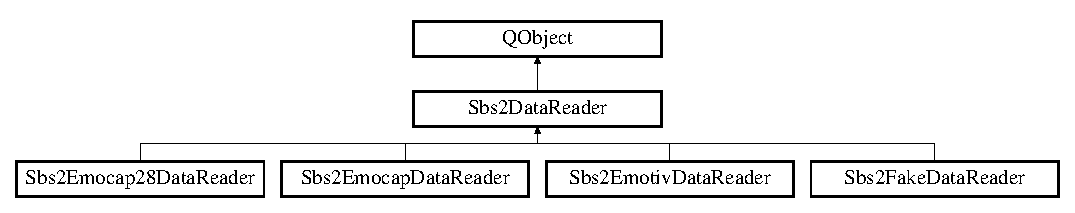
\includegraphics[height=2.413793cm]{classSbs2DataReader}
\end{center}
\end{figure}
\subsection*{Public Slots}
\begin{DoxyCompactItemize}
\item 
virtual void \hyperlink{classSbs2DataReader_adf247d12bc7a9d4ec368c10a6516ee27}{device\-Found} (Q\-Map$<$ Q\-String, Q\-Variant $>$ params)
\item 
virtual void \hyperlink{classSbs2DataReader_a2dd9b209ae967396d82c041b7ea1e494}{device\-Lost} ()
\item 
virtual void \hyperlink{classSbs2DataReader_a1990beb8bea474d074befc259afaf7ed}{about\-To\-Quit} ()
\item 
virtual void \hyperlink{classSbs2DataReader_a2d96f5fd9a29c92799db5ab41ba80bf8}{udp\-Data\-Received} (Q\-Vector$<$ char $\ast$ $>$ $\ast$data, int counter)
\item 
virtual void \hyperlink{classSbs2DataReader_a29d2eea990fe1da78e5f83c34ef2bb84}{udp\-Data\-Received} (Q\-Udp\-Socket $\ast$raw\-Data\-Udp\-Input\-Socket)
\item 
virtual void \hyperlink{classSbs2DataReader_a3dab2a116c2bd5e594ab6f2044d03713}{turn\-Receive\-Udp\-Data\-On} (Q\-String address, int port)
\item 
virtual void \hyperlink{classSbs2DataReader_af30ede5dbff8dd3101bc6a7553d1c2cf}{turn\-Receive\-Udp\-Data\-Off} ()
\end{DoxyCompactItemize}
\subsection*{Signals}
\begin{DoxyCompactItemize}
\item 
void \hyperlink{classSbs2DataReader_af3811e79dd9f544405a5bb83d2c61a9c}{device\-Found\-Signal} (Q\-Map$<$ Q\-String, Q\-Variant $>$ params)
\end{DoxyCompactItemize}
\subsection*{Public Member Functions}
\begin{DoxyCompactItemize}
\item 
\hyperlink{classSbs2DataReader_a722a0ea14fc88b13817701f647c63d7e}{$\sim$\-Sbs2\-Data\-Reader} ()
\end{DoxyCompactItemize}
\subsection*{Protected Member Functions}
\begin{DoxyCompactItemize}
\item 
\hyperlink{classSbs2DataReader_acb12eae29b9e3715e4604a745859c153}{Sbs2\-Data\-Reader} (\hyperlink{classSbs2Callback}{Sbs2\-Callback} $\ast$sbs2\-Callback\-\_\-, int read\-Only\-From\-Network\-\_\-=0, Q\-Object $\ast$parent=0)
\item 
virtual void \hyperlink{classSbs2DataReader_a08efa39d3a0b6a4f8f545a3fbd0998a0}{execute} ()
\end{DoxyCompactItemize}
\subsection*{Protected Attributes}
\begin{DoxyCompactItemize}
\item 
int \hyperlink{classSbs2DataReader_a09c24a1835b3289cc5f7cb5fe975823d}{frames\-Read}
\item 
int \hyperlink{classSbs2DataReader_a65ac7461c3253ec38d8837eac759cf8d}{current\-Index}
\item 
int \hyperlink{classSbs2DataReader_ac7d4147f409871c52e0a49f451f4aedf}{buffer\-Index}
\item 
int \hyperlink{classSbs2DataReader_a40cf787abf8171fcc26384d31e0fa440}{buffer\-Size}
\item 
int \hyperlink{classSbs2DataReader_abf87e9f54439bacc5e9181a7c61394b8}{running}
\item 
\hyperlink{classSbs2Callback}{Sbs2\-Callback} $\ast$ \hyperlink{classSbs2DataReader_a3e6b283fc7ad156341ca90c64139f88a}{sbs2\-Callback}
\item 
int \hyperlink{classSbs2DataReader_a7c66f0a2da31e3c186bfb3ac7da13ecb}{test\-Dummy\-Read}
\item 
\hyperlink{classSbs2NetworkHandler}{Sbs2\-Network\-Handler} $\ast$ \hyperlink{classSbs2DataReader_afb837cc5dbf1d189a64f47e76878bf4c}{sbs2\-Network\-Handler}
\item 
int \hyperlink{classSbs2DataReader_aaef5f0c54d01dec8075721c8367e68c2}{read\-Only\-From\-Network}
\item 
int \hyperlink{classSbs2DataReader_a187026725f6512dda1a579b5876cea83}{last\-Receive\-Raw\-Data\-Counter}
\end{DoxyCompactItemize}


\subsection{Constructor \& Destructor Documentation}
\hypertarget{classSbs2DataReader_a722a0ea14fc88b13817701f647c63d7e}{\index{Sbs2\-Data\-Reader@{Sbs2\-Data\-Reader}!$\sim$\-Sbs2\-Data\-Reader@{$\sim$\-Sbs2\-Data\-Reader}}
\index{$\sim$\-Sbs2\-Data\-Reader@{$\sim$\-Sbs2\-Data\-Reader}!Sbs2DataReader@{Sbs2\-Data\-Reader}}
\subsubsection[{$\sim$\-Sbs2\-Data\-Reader}]{\setlength{\rightskip}{0pt plus 5cm}Sbs2\-Data\-Reader\-::$\sim$\-Sbs2\-Data\-Reader (
\begin{DoxyParamCaption}
{}
\end{DoxyParamCaption}
)}}\label{classSbs2DataReader_a722a0ea14fc88b13817701f647c63d7e}
\hypertarget{classSbs2DataReader_acb12eae29b9e3715e4604a745859c153}{\index{Sbs2\-Data\-Reader@{Sbs2\-Data\-Reader}!Sbs2\-Data\-Reader@{Sbs2\-Data\-Reader}}
\index{Sbs2\-Data\-Reader@{Sbs2\-Data\-Reader}!Sbs2DataReader@{Sbs2\-Data\-Reader}}
\subsubsection[{Sbs2\-Data\-Reader}]{\setlength{\rightskip}{0pt plus 5cm}Sbs2\-Data\-Reader\-::\-Sbs2\-Data\-Reader (
\begin{DoxyParamCaption}
\item[{{\bf Sbs2\-Callback} $\ast$}]{sbs2\-Callback\-\_\-, }
\item[{int}]{read\-Only\-From\-Network\-\_\- = {\ttfamily 0}, }
\item[{Q\-Object $\ast$}]{parent = {\ttfamily 0}}
\end{DoxyParamCaption}
)\hspace{0.3cm}{\ttfamily [protected]}}}\label{classSbs2DataReader_acb12eae29b9e3715e4604a745859c153}


\subsection{Member Function Documentation}
\hypertarget{classSbs2DataReader_a1990beb8bea474d074befc259afaf7ed}{\index{Sbs2\-Data\-Reader@{Sbs2\-Data\-Reader}!about\-To\-Quit@{about\-To\-Quit}}
\index{about\-To\-Quit@{about\-To\-Quit}!Sbs2DataReader@{Sbs2\-Data\-Reader}}
\subsubsection[{about\-To\-Quit}]{\setlength{\rightskip}{0pt plus 5cm}void Sbs2\-Data\-Reader\-::about\-To\-Quit (
\begin{DoxyParamCaption}
{}
\end{DoxyParamCaption}
)\hspace{0.3cm}{\ttfamily [virtual]}, {\ttfamily [slot]}}}\label{classSbs2DataReader_a1990beb8bea474d074befc259afaf7ed}
\hypertarget{classSbs2DataReader_adf247d12bc7a9d4ec368c10a6516ee27}{\index{Sbs2\-Data\-Reader@{Sbs2\-Data\-Reader}!device\-Found@{device\-Found}}
\index{device\-Found@{device\-Found}!Sbs2DataReader@{Sbs2\-Data\-Reader}}
\subsubsection[{device\-Found}]{\setlength{\rightskip}{0pt plus 5cm}void Sbs2\-Data\-Reader\-::device\-Found (
\begin{DoxyParamCaption}
\item[{Q\-Map$<$ Q\-String, Q\-Variant $>$}]{params}
\end{DoxyParamCaption}
)\hspace{0.3cm}{\ttfamily [virtual]}, {\ttfamily [slot]}}}\label{classSbs2DataReader_adf247d12bc7a9d4ec368c10a6516ee27}
\hypertarget{classSbs2DataReader_af3811e79dd9f544405a5bb83d2c61a9c}{\index{Sbs2\-Data\-Reader@{Sbs2\-Data\-Reader}!device\-Found\-Signal@{device\-Found\-Signal}}
\index{device\-Found\-Signal@{device\-Found\-Signal}!Sbs2DataReader@{Sbs2\-Data\-Reader}}
\subsubsection[{device\-Found\-Signal}]{\setlength{\rightskip}{0pt plus 5cm}void Sbs2\-Data\-Reader\-::device\-Found\-Signal (
\begin{DoxyParamCaption}
\item[{Q\-Map$<$ Q\-String, Q\-Variant $>$}]{params}
\end{DoxyParamCaption}
)\hspace{0.3cm}{\ttfamily [signal]}}}\label{classSbs2DataReader_af3811e79dd9f544405a5bb83d2c61a9c}
\hypertarget{classSbs2DataReader_a2dd9b209ae967396d82c041b7ea1e494}{\index{Sbs2\-Data\-Reader@{Sbs2\-Data\-Reader}!device\-Lost@{device\-Lost}}
\index{device\-Lost@{device\-Lost}!Sbs2DataReader@{Sbs2\-Data\-Reader}}
\subsubsection[{device\-Lost}]{\setlength{\rightskip}{0pt plus 5cm}void Sbs2\-Data\-Reader\-::device\-Lost (
\begin{DoxyParamCaption}
{}
\end{DoxyParamCaption}
)\hspace{0.3cm}{\ttfamily [virtual]}, {\ttfamily [slot]}}}\label{classSbs2DataReader_a2dd9b209ae967396d82c041b7ea1e494}
\hypertarget{classSbs2DataReader_a08efa39d3a0b6a4f8f545a3fbd0998a0}{\index{Sbs2\-Data\-Reader@{Sbs2\-Data\-Reader}!execute@{execute}}
\index{execute@{execute}!Sbs2DataReader@{Sbs2\-Data\-Reader}}
\subsubsection[{execute}]{\setlength{\rightskip}{0pt plus 5cm}void Sbs2\-Data\-Reader\-::execute (
\begin{DoxyParamCaption}
{}
\end{DoxyParamCaption}
)\hspace{0.3cm}{\ttfamily [protected]}, {\ttfamily [virtual]}}}\label{classSbs2DataReader_a08efa39d3a0b6a4f8f545a3fbd0998a0}
\hypertarget{classSbs2DataReader_af30ede5dbff8dd3101bc6a7553d1c2cf}{\index{Sbs2\-Data\-Reader@{Sbs2\-Data\-Reader}!turn\-Receive\-Udp\-Data\-Off@{turn\-Receive\-Udp\-Data\-Off}}
\index{turn\-Receive\-Udp\-Data\-Off@{turn\-Receive\-Udp\-Data\-Off}!Sbs2DataReader@{Sbs2\-Data\-Reader}}
\subsubsection[{turn\-Receive\-Udp\-Data\-Off}]{\setlength{\rightskip}{0pt plus 5cm}void Sbs2\-Data\-Reader\-::turn\-Receive\-Udp\-Data\-Off (
\begin{DoxyParamCaption}
{}
\end{DoxyParamCaption}
)\hspace{0.3cm}{\ttfamily [virtual]}, {\ttfamily [slot]}}}\label{classSbs2DataReader_af30ede5dbff8dd3101bc6a7553d1c2cf}
\hypertarget{classSbs2DataReader_a3dab2a116c2bd5e594ab6f2044d03713}{\index{Sbs2\-Data\-Reader@{Sbs2\-Data\-Reader}!turn\-Receive\-Udp\-Data\-On@{turn\-Receive\-Udp\-Data\-On}}
\index{turn\-Receive\-Udp\-Data\-On@{turn\-Receive\-Udp\-Data\-On}!Sbs2DataReader@{Sbs2\-Data\-Reader}}
\subsubsection[{turn\-Receive\-Udp\-Data\-On}]{\setlength{\rightskip}{0pt plus 5cm}void Sbs2\-Data\-Reader\-::turn\-Receive\-Udp\-Data\-On (
\begin{DoxyParamCaption}
\item[{Q\-String}]{address, }
\item[{int}]{port}
\end{DoxyParamCaption}
)\hspace{0.3cm}{\ttfamily [virtual]}, {\ttfamily [slot]}}}\label{classSbs2DataReader_a3dab2a116c2bd5e594ab6f2044d03713}
\hypertarget{classSbs2DataReader_a2d96f5fd9a29c92799db5ab41ba80bf8}{\index{Sbs2\-Data\-Reader@{Sbs2\-Data\-Reader}!udp\-Data\-Received@{udp\-Data\-Received}}
\index{udp\-Data\-Received@{udp\-Data\-Received}!Sbs2DataReader@{Sbs2\-Data\-Reader}}
\subsubsection[{udp\-Data\-Received}]{\setlength{\rightskip}{0pt plus 5cm}void Sbs2\-Data\-Reader\-::udp\-Data\-Received (
\begin{DoxyParamCaption}
\item[{Q\-Vector$<$ char $\ast$ $>$ $\ast$}]{data, }
\item[{int}]{counter}
\end{DoxyParamCaption}
)\hspace{0.3cm}{\ttfamily [virtual]}, {\ttfamily [slot]}}}\label{classSbs2DataReader_a2d96f5fd9a29c92799db5ab41ba80bf8}
\hypertarget{classSbs2DataReader_a29d2eea990fe1da78e5f83c34ef2bb84}{\index{Sbs2\-Data\-Reader@{Sbs2\-Data\-Reader}!udp\-Data\-Received@{udp\-Data\-Received}}
\index{udp\-Data\-Received@{udp\-Data\-Received}!Sbs2DataReader@{Sbs2\-Data\-Reader}}
\subsubsection[{udp\-Data\-Received}]{\setlength{\rightskip}{0pt plus 5cm}void Sbs2\-Data\-Reader\-::udp\-Data\-Received (
\begin{DoxyParamCaption}
\item[{Q\-Udp\-Socket $\ast$}]{raw\-Data\-Udp\-Input\-Socket}
\end{DoxyParamCaption}
)\hspace{0.3cm}{\ttfamily [virtual]}, {\ttfamily [slot]}}}\label{classSbs2DataReader_a29d2eea990fe1da78e5f83c34ef2bb84}


\subsection{Member Data Documentation}
\hypertarget{classSbs2DataReader_ac7d4147f409871c52e0a49f451f4aedf}{\index{Sbs2\-Data\-Reader@{Sbs2\-Data\-Reader}!buffer\-Index@{buffer\-Index}}
\index{buffer\-Index@{buffer\-Index}!Sbs2DataReader@{Sbs2\-Data\-Reader}}
\subsubsection[{buffer\-Index}]{\setlength{\rightskip}{0pt plus 5cm}int Sbs2\-Data\-Reader\-::buffer\-Index\hspace{0.3cm}{\ttfamily [protected]}}}\label{classSbs2DataReader_ac7d4147f409871c52e0a49f451f4aedf}
\hypertarget{classSbs2DataReader_a40cf787abf8171fcc26384d31e0fa440}{\index{Sbs2\-Data\-Reader@{Sbs2\-Data\-Reader}!buffer\-Size@{buffer\-Size}}
\index{buffer\-Size@{buffer\-Size}!Sbs2DataReader@{Sbs2\-Data\-Reader}}
\subsubsection[{buffer\-Size}]{\setlength{\rightskip}{0pt plus 5cm}int Sbs2\-Data\-Reader\-::buffer\-Size\hspace{0.3cm}{\ttfamily [protected]}}}\label{classSbs2DataReader_a40cf787abf8171fcc26384d31e0fa440}
\hypertarget{classSbs2DataReader_a65ac7461c3253ec38d8837eac759cf8d}{\index{Sbs2\-Data\-Reader@{Sbs2\-Data\-Reader}!current\-Index@{current\-Index}}
\index{current\-Index@{current\-Index}!Sbs2DataReader@{Sbs2\-Data\-Reader}}
\subsubsection[{current\-Index}]{\setlength{\rightskip}{0pt plus 5cm}int Sbs2\-Data\-Reader\-::current\-Index\hspace{0.3cm}{\ttfamily [protected]}}}\label{classSbs2DataReader_a65ac7461c3253ec38d8837eac759cf8d}
\hypertarget{classSbs2DataReader_a09c24a1835b3289cc5f7cb5fe975823d}{\index{Sbs2\-Data\-Reader@{Sbs2\-Data\-Reader}!frames\-Read@{frames\-Read}}
\index{frames\-Read@{frames\-Read}!Sbs2DataReader@{Sbs2\-Data\-Reader}}
\subsubsection[{frames\-Read}]{\setlength{\rightskip}{0pt plus 5cm}int Sbs2\-Data\-Reader\-::frames\-Read\hspace{0.3cm}{\ttfamily [protected]}}}\label{classSbs2DataReader_a09c24a1835b3289cc5f7cb5fe975823d}
\hypertarget{classSbs2DataReader_a187026725f6512dda1a579b5876cea83}{\index{Sbs2\-Data\-Reader@{Sbs2\-Data\-Reader}!last\-Receive\-Raw\-Data\-Counter@{last\-Receive\-Raw\-Data\-Counter}}
\index{last\-Receive\-Raw\-Data\-Counter@{last\-Receive\-Raw\-Data\-Counter}!Sbs2DataReader@{Sbs2\-Data\-Reader}}
\subsubsection[{last\-Receive\-Raw\-Data\-Counter}]{\setlength{\rightskip}{0pt plus 5cm}int Sbs2\-Data\-Reader\-::last\-Receive\-Raw\-Data\-Counter\hspace{0.3cm}{\ttfamily [protected]}}}\label{classSbs2DataReader_a187026725f6512dda1a579b5876cea83}
\hypertarget{classSbs2DataReader_aaef5f0c54d01dec8075721c8367e68c2}{\index{Sbs2\-Data\-Reader@{Sbs2\-Data\-Reader}!read\-Only\-From\-Network@{read\-Only\-From\-Network}}
\index{read\-Only\-From\-Network@{read\-Only\-From\-Network}!Sbs2DataReader@{Sbs2\-Data\-Reader}}
\subsubsection[{read\-Only\-From\-Network}]{\setlength{\rightskip}{0pt plus 5cm}int Sbs2\-Data\-Reader\-::read\-Only\-From\-Network\hspace{0.3cm}{\ttfamily [protected]}}}\label{classSbs2DataReader_aaef5f0c54d01dec8075721c8367e68c2}
\hypertarget{classSbs2DataReader_abf87e9f54439bacc5e9181a7c61394b8}{\index{Sbs2\-Data\-Reader@{Sbs2\-Data\-Reader}!running@{running}}
\index{running@{running}!Sbs2DataReader@{Sbs2\-Data\-Reader}}
\subsubsection[{running}]{\setlength{\rightskip}{0pt plus 5cm}int Sbs2\-Data\-Reader\-::running\hspace{0.3cm}{\ttfamily [protected]}}}\label{classSbs2DataReader_abf87e9f54439bacc5e9181a7c61394b8}
\hypertarget{classSbs2DataReader_a3e6b283fc7ad156341ca90c64139f88a}{\index{Sbs2\-Data\-Reader@{Sbs2\-Data\-Reader}!sbs2\-Callback@{sbs2\-Callback}}
\index{sbs2\-Callback@{sbs2\-Callback}!Sbs2DataReader@{Sbs2\-Data\-Reader}}
\subsubsection[{sbs2\-Callback}]{\setlength{\rightskip}{0pt plus 5cm}{\bf Sbs2\-Callback}$\ast$ Sbs2\-Data\-Reader\-::sbs2\-Callback\hspace{0.3cm}{\ttfamily [protected]}}}\label{classSbs2DataReader_a3e6b283fc7ad156341ca90c64139f88a}
\hypertarget{classSbs2DataReader_afb837cc5dbf1d189a64f47e76878bf4c}{\index{Sbs2\-Data\-Reader@{Sbs2\-Data\-Reader}!sbs2\-Network\-Handler@{sbs2\-Network\-Handler}}
\index{sbs2\-Network\-Handler@{sbs2\-Network\-Handler}!Sbs2DataReader@{Sbs2\-Data\-Reader}}
\subsubsection[{sbs2\-Network\-Handler}]{\setlength{\rightskip}{0pt plus 5cm}{\bf Sbs2\-Network\-Handler}$\ast$ Sbs2\-Data\-Reader\-::sbs2\-Network\-Handler\hspace{0.3cm}{\ttfamily [protected]}}}\label{classSbs2DataReader_afb837cc5dbf1d189a64f47e76878bf4c}
\hypertarget{classSbs2DataReader_a7c66f0a2da31e3c186bfb3ac7da13ecb}{\index{Sbs2\-Data\-Reader@{Sbs2\-Data\-Reader}!test\-Dummy\-Read@{test\-Dummy\-Read}}
\index{test\-Dummy\-Read@{test\-Dummy\-Read}!Sbs2DataReader@{Sbs2\-Data\-Reader}}
\subsubsection[{test\-Dummy\-Read}]{\setlength{\rightskip}{0pt plus 5cm}int Sbs2\-Data\-Reader\-::test\-Dummy\-Read\hspace{0.3cm}{\ttfamily [protected]}}}\label{classSbs2DataReader_a7c66f0a2da31e3c186bfb3ac7da13ecb}


The documentation for this class was generated from the following files\-:\begin{DoxyCompactItemize}
\item 
/media/philipjhj/\-Data/\-One\-Drive/\-Studie/\-Studenterprogrammør/\-S\-B\-S3/smartphonebrainscanner2-\/core/src/hardware/\hyperlink{sbs2datareader_8h}{sbs2datareader.\-h}\item 
/media/philipjhj/\-Data/\-One\-Drive/\-Studie/\-Studenterprogrammør/\-S\-B\-S3/smartphonebrainscanner2-\/core/src/hardware/\hyperlink{sbs2datareader_8cpp}{sbs2datareader.\-cpp}\end{DoxyCompactItemize}

\hypertarget{classSbs2Emocap28DataContainer}{\section{Sbs2\-Emocap28\-Data\-Container Class Reference}
\label{classSbs2Emocap28DataContainer}\index{Sbs2\-Emocap28\-Data\-Container@{Sbs2\-Emocap28\-Data\-Container}}
}


{\ttfamily \#include $<$sbs2emocap28datareader.\-h$>$}

\subsection*{Public Member Functions}
\begin{DoxyCompactItemize}
\item 
\hyperlink{classSbs2Emocap28DataContainer_a4a808fc6705415a114d30a7d0bb17810}{Sbs2\-Emocap28\-Data\-Container} ()
\item 
void \hyperlink{classSbs2Emocap28DataContainer_a5729680a3fd18a5e98e4ec439f9d3812}{update} (char $\ast$data\-\_\-, int counter\-\_\-)
\end{DoxyCompactItemize}
\subsection*{Public Attributes}
\begin{DoxyCompactItemize}
\item 
char $\ast$ \hyperlink{classSbs2Emocap28DataContainer_a75d846cbb3de36cd05e33bf69638cda5}{data}
\item 
int \hyperlink{classSbs2Emocap28DataContainer_adb1eef2558c19b1c1d2b4e53a72f2bc8}{counter}
\end{DoxyCompactItemize}


\subsection{Detailed Description}
Smartphone Brain Scanner 2 License Agreement (M\-I\-T License)

Copyright (c) 2012 Arkadiusz Stopczynski, Jakob Eg Larsen, Carsten Stahlhut, Michael Kai Petersen, Lars Kai Hansen. Technical University of Denmark, \hyperlink{namespaceDTU}{D\-T\-U} Informatics, Cognitive Systems Section. \href{http://code.google.com/p/smartphonebrainscanner2}{\tt http\-://code.\-google.\-com/p/smartphonebrainscanner2}

Permission is hereby granted, free of charge, to any person obtaining a copy of this software and associated documentation files (the \char`\"{}\-Software\char`\"{}), to deal in the Software without restriction, including without limitation the rights to use, copy, modify, merge, publish, distribute, sublicense, and/or sell copies of the Software, and to permit persons to whom the Software is furnished to do so, subject to the following conditions\-:

The above copyright notice and this permission notice shall be included in all copies or substantial portions of the Software.

T\-H\-E S\-O\-F\-T\-W\-A\-R\-E I\-S P\-R\-O\-V\-I\-D\-E\-D \char`\"{}\-A\-S I\-S\char`\"{}, W\-I\-T\-H\-O\-U\-T W\-A\-R\-R\-A\-N\-T\-Y O\-F A\-N\-Y K\-I\-N\-D, E\-X\-P\-R\-E\-S\-S O\-R I\-M\-P\-L\-I\-E\-D, I\-N\-C\-L\-U\-D\-I\-N\-G B\-U\-T N\-O\-T L\-I\-M\-I\-T\-E\-D T\-O T\-H\-E W\-A\-R\-R\-A\-N\-T\-I\-E\-S O\-F M\-E\-R\-C\-H\-A\-N\-T\-A\-B\-I\-L\-I\-T\-Y, F\-I\-T\-N\-E\-S\-S F\-O\-R A P\-A\-R\-T\-I\-C\-U\-L\-A\-R P\-U\-R\-P\-O\-S\-E A\-N\-D N\-O\-N\-I\-N\-F\-R\-I\-N\-G\-E\-M\-E\-N\-T. I\-N N\-O E\-V\-E\-N\-T S\-H\-A\-L\-L T\-H\-E A\-U\-T\-H\-O\-R\-S O\-R C\-O\-P\-Y\-R\-I\-G\-H\-T H\-O\-L\-D\-E\-R\-S B\-E L\-I\-A\-B\-L\-E F\-O\-R A\-N\-Y C\-L\-A\-I\-M, D\-A\-M\-A\-G\-E\-S O\-R O\-T\-H\-E\-R L\-I\-A\-B\-I\-L\-I\-T\-Y, W\-H\-E\-T\-H\-E\-R I\-N A\-N A\-C\-T\-I\-O\-N O\-F C\-O\-N\-T\-R\-A\-C\-T, T\-O\-R\-T O\-R O\-T\-H\-E\-R\-W\-I\-S\-E, A\-R\-I\-S\-I\-N\-G F\-R\-O\-M, O\-U\-T O\-F O\-R I\-N C\-O\-N\-N\-E\-C\-T\-I\-O\-N W\-I\-T\-H T\-H\-E S\-O\-F\-T\-W\-A\-R\-E O\-R T\-H\-E U\-S\-E O\-R O\-T\-H\-E\-R D\-E\-A\-L\-I\-N\-G\-S I\-N T\-H\-E S\-O\-F\-T\-W\-A\-R\-E. 

\subsection{Constructor \& Destructor Documentation}
\hypertarget{classSbs2Emocap28DataContainer_a4a808fc6705415a114d30a7d0bb17810}{\index{Sbs2\-Emocap28\-Data\-Container@{Sbs2\-Emocap28\-Data\-Container}!Sbs2\-Emocap28\-Data\-Container@{Sbs2\-Emocap28\-Data\-Container}}
\index{Sbs2\-Emocap28\-Data\-Container@{Sbs2\-Emocap28\-Data\-Container}!Sbs2Emocap28DataContainer@{Sbs2\-Emocap28\-Data\-Container}}
\subsubsection[{Sbs2\-Emocap28\-Data\-Container}]{\setlength{\rightskip}{0pt plus 5cm}Sbs2\-Emocap28\-Data\-Container\-::\-Sbs2\-Emocap28\-Data\-Container (
\begin{DoxyParamCaption}
{}
\end{DoxyParamCaption}
)\hspace{0.3cm}{\ttfamily [inline]}}}\label{classSbs2Emocap28DataContainer_a4a808fc6705415a114d30a7d0bb17810}


\subsection{Member Function Documentation}
\hypertarget{classSbs2Emocap28DataContainer_a5729680a3fd18a5e98e4ec439f9d3812}{\index{Sbs2\-Emocap28\-Data\-Container@{Sbs2\-Emocap28\-Data\-Container}!update@{update}}
\index{update@{update}!Sbs2Emocap28DataContainer@{Sbs2\-Emocap28\-Data\-Container}}
\subsubsection[{update}]{\setlength{\rightskip}{0pt plus 5cm}void Sbs2\-Emocap28\-Data\-Container\-::update (
\begin{DoxyParamCaption}
\item[{char $\ast$}]{data\-\_\-, }
\item[{int}]{counter\-\_\-}
\end{DoxyParamCaption}
)}}\label{classSbs2Emocap28DataContainer_a5729680a3fd18a5e98e4ec439f9d3812}


\subsection{Member Data Documentation}
\hypertarget{classSbs2Emocap28DataContainer_adb1eef2558c19b1c1d2b4e53a72f2bc8}{\index{Sbs2\-Emocap28\-Data\-Container@{Sbs2\-Emocap28\-Data\-Container}!counter@{counter}}
\index{counter@{counter}!Sbs2Emocap28DataContainer@{Sbs2\-Emocap28\-Data\-Container}}
\subsubsection[{counter}]{\setlength{\rightskip}{0pt plus 5cm}int Sbs2\-Emocap28\-Data\-Container\-::counter}}\label{classSbs2Emocap28DataContainer_adb1eef2558c19b1c1d2b4e53a72f2bc8}
\hypertarget{classSbs2Emocap28DataContainer_a75d846cbb3de36cd05e33bf69638cda5}{\index{Sbs2\-Emocap28\-Data\-Container@{Sbs2\-Emocap28\-Data\-Container}!data@{data}}
\index{data@{data}!Sbs2Emocap28DataContainer@{Sbs2\-Emocap28\-Data\-Container}}
\subsubsection[{data}]{\setlength{\rightskip}{0pt plus 5cm}char$\ast$ Sbs2\-Emocap28\-Data\-Container\-::data}}\label{classSbs2Emocap28DataContainer_a75d846cbb3de36cd05e33bf69638cda5}


The documentation for this class was generated from the following files\-:\begin{DoxyCompactItemize}
\item 
/media/philipjhj/\-Data/\-One\-Drive/\-Studie/\-Studenterprogrammør/\-S\-B\-S3/smartphonebrainscanner2-\/core/src/hardware/emocap28/\hyperlink{sbs2emocap28datareader_8h}{sbs2emocap28datareader.\-h}\item 
/media/philipjhj/\-Data/\-One\-Drive/\-Studie/\-Studenterprogrammør/\-S\-B\-S3/smartphonebrainscanner2-\/core/src/hardware/emocap28/\hyperlink{sbs2emocap28datareader_8cpp}{sbs2emocap28datareader.\-cpp}\end{DoxyCompactItemize}

\hypertarget{classSbs2Emocap28DataReader}{\section{Sbs2\-Emocap28\-Data\-Reader Class Reference}
\label{classSbs2Emocap28DataReader}\index{Sbs2\-Emocap28\-Data\-Reader@{Sbs2\-Emocap28\-Data\-Reader}}
}


{\ttfamily \#include $<$sbs2emocap28datareader.\-h$>$}

Inheritance diagram for Sbs2\-Emocap28\-Data\-Reader\-:\begin{figure}[H]
\begin{center}
\leavevmode
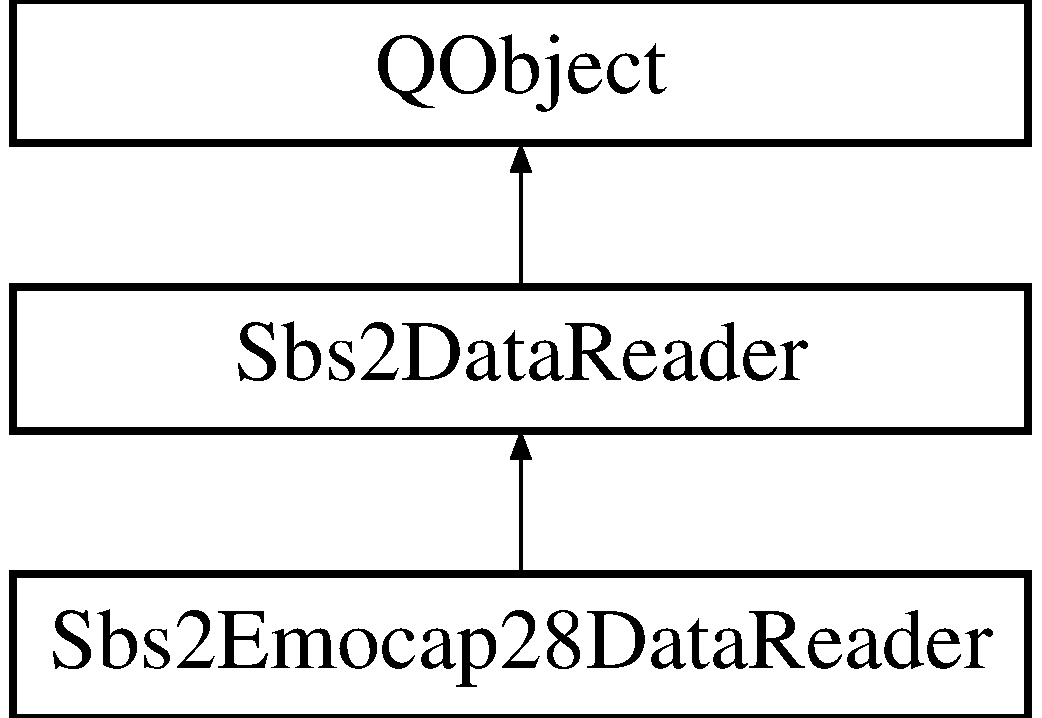
\includegraphics[height=3.000000cm]{classSbs2Emocap28DataReader}
\end{center}
\end{figure}
\subsection*{Public Slots}
\begin{DoxyCompactItemize}
\item 
void \hyperlink{classSbs2Emocap28DataReader_ab845451927a5b0183730f3eb5a09f146}{device\-Found} (Q\-Map$<$ Q\-String, Q\-Variant $>$ params)
\item 
void \hyperlink{classSbs2Emocap28DataReader_ae8677a65973a4ee21ff2b0103a1e4c2e}{device\-Lost} ()
\item 
void \hyperlink{classSbs2Emocap28DataReader_a5ff03b12f1c22a5a35f77cdcb627526e}{about\-To\-Quit} ()
\item 
void \hyperlink{classSbs2Emocap28DataReader_a3670f62d390b425f58dc328d887f4e40}{udp\-Data\-Received} (Q\-Vector$<$ char $\ast$ $>$ $\ast$data, int counter)
\item 
void \hyperlink{classSbs2Emocap28DataReader_a0a5161afb5e369562c58c5630ed021f8}{udp\-Data\-Received} (Q\-Udp\-Socket $\ast$raw\-Data\-Udp\-Input\-Socket)
\item 
void \hyperlink{classSbs2Emocap28DataReader_a9bf0852e3e8a66e3d852a53397a034fc}{turn\-Receive\-Udp\-Data\-On} (Q\-String address, int port)
\item 
void \hyperlink{classSbs2Emocap28DataReader_ae5dce4cfc0e8e50af6b2e6c87ba212e1}{turn\-Receive\-Udp\-Data\-Off} ()
\end{DoxyCompactItemize}
\subsection*{Signals}
\begin{DoxyCompactItemize}
\item 
void \hyperlink{classSbs2Emocap28DataReader_a90da90e617c1b65bea974ad632bfe6dc}{amp1\-Found\-Signal} (Q\-Variant number, Q\-Variant path, Q\-Variant serial\-Number)
\item 
void \hyperlink{classSbs2Emocap28DataReader_ae66309bad3418ff624b97d4fe964a4bc}{amp2\-Found\-Signal} (Q\-Variant number, Q\-Variant path, Q\-Variant serial\-Number)
\item 
void \hyperlink{classSbs2Emocap28DataReader_a8a34d2659ebb064fd9dfbbeb8e885f41}{ready\-For\-Data} ()
\item 
void \hyperlink{classSbs2Emocap28DataReader_a768d1a019c7c5f491161e733a2b0282a}{in\-Mapping\-Signal} ()
\item 
void \hyperlink{classSbs2Emocap28DataReader_aea641bcfd2e46b07c9025fc2a05cabf8}{mapping\-Successful} (int mapping)
\item 
void \hyperlink{classSbs2Emocap28DataReader_a8ffaf86ba99e47b332afe46805567374}{mapping\-Failed} ()
\item 
void \hyperlink{classSbs2Emocap28DataReader_a1ccc02a646e7bbac4752bb4544aea6a3}{aligned\-Signal} (int mapping, int mapping\-Alignment, int mapping\-Corr)
\end{DoxyCompactItemize}
\subsection*{Public Member Functions}
\begin{DoxyCompactItemize}
\item 
\hyperlink{classSbs2Emocap28DataReader_a8ccc336f89762cef94be3cb1d2ad7b7a}{$\sim$\-Sbs2\-Emocap28\-Data\-Reader} ()
\end{DoxyCompactItemize}
\subsection*{Static Public Member Functions}
\begin{DoxyCompactItemize}
\item 
static \hyperlink{classSbs2Emocap28DataReader}{Sbs2\-Emocap28\-Data\-Reader} $\ast$ \hyperlink{classSbs2Emocap28DataReader_ae4370297a7212086bc8f5c1e452c769d}{New} (\hyperlink{classSbs2Callback}{Sbs2\-Callback} $\ast$sbs2\-Callback\-\_\-, int read\-Only\-From\-Network\-\_\-=0, Q\-Object $\ast$parent=0)
\end{DoxyCompactItemize}
\subsection*{Additional Inherited Members}


\subsection{Constructor \& Destructor Documentation}
\hypertarget{classSbs2Emocap28DataReader_a8ccc336f89762cef94be3cb1d2ad7b7a}{\index{Sbs2\-Emocap28\-Data\-Reader@{Sbs2\-Emocap28\-Data\-Reader}!$\sim$\-Sbs2\-Emocap28\-Data\-Reader@{$\sim$\-Sbs2\-Emocap28\-Data\-Reader}}
\index{$\sim$\-Sbs2\-Emocap28\-Data\-Reader@{$\sim$\-Sbs2\-Emocap28\-Data\-Reader}!Sbs2Emocap28DataReader@{Sbs2\-Emocap28\-Data\-Reader}}
\subsubsection[{$\sim$\-Sbs2\-Emocap28\-Data\-Reader}]{\setlength{\rightskip}{0pt plus 5cm}Sbs2\-Emocap28\-Data\-Reader\-::$\sim$\-Sbs2\-Emocap28\-Data\-Reader (
\begin{DoxyParamCaption}
{}
\end{DoxyParamCaption}
)}}\label{classSbs2Emocap28DataReader_a8ccc336f89762cef94be3cb1d2ad7b7a}


\subsection{Member Function Documentation}
\hypertarget{classSbs2Emocap28DataReader_a5ff03b12f1c22a5a35f77cdcb627526e}{\index{Sbs2\-Emocap28\-Data\-Reader@{Sbs2\-Emocap28\-Data\-Reader}!about\-To\-Quit@{about\-To\-Quit}}
\index{about\-To\-Quit@{about\-To\-Quit}!Sbs2Emocap28DataReader@{Sbs2\-Emocap28\-Data\-Reader}}
\subsubsection[{about\-To\-Quit}]{\setlength{\rightskip}{0pt plus 5cm}void Sbs2\-Emocap28\-Data\-Reader\-::about\-To\-Quit (
\begin{DoxyParamCaption}
{}
\end{DoxyParamCaption}
)\hspace{0.3cm}{\ttfamily [slot]}}}\label{classSbs2Emocap28DataReader_a5ff03b12f1c22a5a35f77cdcb627526e}
\hypertarget{classSbs2Emocap28DataReader_a1ccc02a646e7bbac4752bb4544aea6a3}{\index{Sbs2\-Emocap28\-Data\-Reader@{Sbs2\-Emocap28\-Data\-Reader}!aligned\-Signal@{aligned\-Signal}}
\index{aligned\-Signal@{aligned\-Signal}!Sbs2Emocap28DataReader@{Sbs2\-Emocap28\-Data\-Reader}}
\subsubsection[{aligned\-Signal}]{\setlength{\rightskip}{0pt plus 5cm}void Sbs2\-Emocap28\-Data\-Reader\-::aligned\-Signal (
\begin{DoxyParamCaption}
\item[{int}]{mapping, }
\item[{int}]{mapping\-Alignment, }
\item[{int}]{mapping\-Corr}
\end{DoxyParamCaption}
)\hspace{0.3cm}{\ttfamily [signal]}}}\label{classSbs2Emocap28DataReader_a1ccc02a646e7bbac4752bb4544aea6a3}
\hypertarget{classSbs2Emocap28DataReader_a90da90e617c1b65bea974ad632bfe6dc}{\index{Sbs2\-Emocap28\-Data\-Reader@{Sbs2\-Emocap28\-Data\-Reader}!amp1\-Found\-Signal@{amp1\-Found\-Signal}}
\index{amp1\-Found\-Signal@{amp1\-Found\-Signal}!Sbs2Emocap28DataReader@{Sbs2\-Emocap28\-Data\-Reader}}
\subsubsection[{amp1\-Found\-Signal}]{\setlength{\rightskip}{0pt plus 5cm}void Sbs2\-Emocap28\-Data\-Reader\-::amp1\-Found\-Signal (
\begin{DoxyParamCaption}
\item[{Q\-Variant}]{number, }
\item[{Q\-Variant}]{path, }
\item[{Q\-Variant}]{serial\-Number}
\end{DoxyParamCaption}
)\hspace{0.3cm}{\ttfamily [signal]}}}\label{classSbs2Emocap28DataReader_a90da90e617c1b65bea974ad632bfe6dc}
\hypertarget{classSbs2Emocap28DataReader_ae66309bad3418ff624b97d4fe964a4bc}{\index{Sbs2\-Emocap28\-Data\-Reader@{Sbs2\-Emocap28\-Data\-Reader}!amp2\-Found\-Signal@{amp2\-Found\-Signal}}
\index{amp2\-Found\-Signal@{amp2\-Found\-Signal}!Sbs2Emocap28DataReader@{Sbs2\-Emocap28\-Data\-Reader}}
\subsubsection[{amp2\-Found\-Signal}]{\setlength{\rightskip}{0pt plus 5cm}void Sbs2\-Emocap28\-Data\-Reader\-::amp2\-Found\-Signal (
\begin{DoxyParamCaption}
\item[{Q\-Variant}]{number, }
\item[{Q\-Variant}]{path, }
\item[{Q\-Variant}]{serial\-Number}
\end{DoxyParamCaption}
)\hspace{0.3cm}{\ttfamily [signal]}}}\label{classSbs2Emocap28DataReader_ae66309bad3418ff624b97d4fe964a4bc}
\hypertarget{classSbs2Emocap28DataReader_ab845451927a5b0183730f3eb5a09f146}{\index{Sbs2\-Emocap28\-Data\-Reader@{Sbs2\-Emocap28\-Data\-Reader}!device\-Found@{device\-Found}}
\index{device\-Found@{device\-Found}!Sbs2Emocap28DataReader@{Sbs2\-Emocap28\-Data\-Reader}}
\subsubsection[{device\-Found}]{\setlength{\rightskip}{0pt plus 5cm}void Sbs2\-Emocap28\-Data\-Reader\-::device\-Found (
\begin{DoxyParamCaption}
\item[{Q\-Map$<$ Q\-String, Q\-Variant $>$}]{params}
\end{DoxyParamCaption}
)\hspace{0.3cm}{\ttfamily [slot]}}}\label{classSbs2Emocap28DataReader_ab845451927a5b0183730f3eb5a09f146}
\hypertarget{classSbs2Emocap28DataReader_ae8677a65973a4ee21ff2b0103a1e4c2e}{\index{Sbs2\-Emocap28\-Data\-Reader@{Sbs2\-Emocap28\-Data\-Reader}!device\-Lost@{device\-Lost}}
\index{device\-Lost@{device\-Lost}!Sbs2Emocap28DataReader@{Sbs2\-Emocap28\-Data\-Reader}}
\subsubsection[{device\-Lost}]{\setlength{\rightskip}{0pt plus 5cm}void Sbs2\-Emocap28\-Data\-Reader\-::device\-Lost (
\begin{DoxyParamCaption}
{}
\end{DoxyParamCaption}
)\hspace{0.3cm}{\ttfamily [slot]}}}\label{classSbs2Emocap28DataReader_ae8677a65973a4ee21ff2b0103a1e4c2e}
\hypertarget{classSbs2Emocap28DataReader_a768d1a019c7c5f491161e733a2b0282a}{\index{Sbs2\-Emocap28\-Data\-Reader@{Sbs2\-Emocap28\-Data\-Reader}!in\-Mapping\-Signal@{in\-Mapping\-Signal}}
\index{in\-Mapping\-Signal@{in\-Mapping\-Signal}!Sbs2Emocap28DataReader@{Sbs2\-Emocap28\-Data\-Reader}}
\subsubsection[{in\-Mapping\-Signal}]{\setlength{\rightskip}{0pt plus 5cm}void Sbs2\-Emocap28\-Data\-Reader\-::in\-Mapping\-Signal (
\begin{DoxyParamCaption}
{}
\end{DoxyParamCaption}
)\hspace{0.3cm}{\ttfamily [signal]}}}\label{classSbs2Emocap28DataReader_a768d1a019c7c5f491161e733a2b0282a}
\hypertarget{classSbs2Emocap28DataReader_a8ffaf86ba99e47b332afe46805567374}{\index{Sbs2\-Emocap28\-Data\-Reader@{Sbs2\-Emocap28\-Data\-Reader}!mapping\-Failed@{mapping\-Failed}}
\index{mapping\-Failed@{mapping\-Failed}!Sbs2Emocap28DataReader@{Sbs2\-Emocap28\-Data\-Reader}}
\subsubsection[{mapping\-Failed}]{\setlength{\rightskip}{0pt plus 5cm}void Sbs2\-Emocap28\-Data\-Reader\-::mapping\-Failed (
\begin{DoxyParamCaption}
{}
\end{DoxyParamCaption}
)\hspace{0.3cm}{\ttfamily [signal]}}}\label{classSbs2Emocap28DataReader_a8ffaf86ba99e47b332afe46805567374}
\hypertarget{classSbs2Emocap28DataReader_aea641bcfd2e46b07c9025fc2a05cabf8}{\index{Sbs2\-Emocap28\-Data\-Reader@{Sbs2\-Emocap28\-Data\-Reader}!mapping\-Successful@{mapping\-Successful}}
\index{mapping\-Successful@{mapping\-Successful}!Sbs2Emocap28DataReader@{Sbs2\-Emocap28\-Data\-Reader}}
\subsubsection[{mapping\-Successful}]{\setlength{\rightskip}{0pt plus 5cm}void Sbs2\-Emocap28\-Data\-Reader\-::mapping\-Successful (
\begin{DoxyParamCaption}
\item[{int}]{mapping}
\end{DoxyParamCaption}
)\hspace{0.3cm}{\ttfamily [signal]}}}\label{classSbs2Emocap28DataReader_aea641bcfd2e46b07c9025fc2a05cabf8}
\hypertarget{classSbs2Emocap28DataReader_ae4370297a7212086bc8f5c1e452c769d}{\index{Sbs2\-Emocap28\-Data\-Reader@{Sbs2\-Emocap28\-Data\-Reader}!New@{New}}
\index{New@{New}!Sbs2Emocap28DataReader@{Sbs2\-Emocap28\-Data\-Reader}}
\subsubsection[{New}]{\setlength{\rightskip}{0pt plus 5cm}{\bf Sbs2\-Emocap28\-Data\-Reader} $\ast$ Sbs2\-Emocap28\-Data\-Reader\-::\-New (
\begin{DoxyParamCaption}
\item[{{\bf Sbs2\-Callback} $\ast$}]{sbs2\-Callback\-\_\-, }
\item[{int}]{read\-Only\-From\-Network\-\_\- = {\ttfamily 0}, }
\item[{Q\-Object $\ast$}]{parent = {\ttfamily 0}}
\end{DoxyParamCaption}
)\hspace{0.3cm}{\ttfamily [static]}}}\label{classSbs2Emocap28DataReader_ae4370297a7212086bc8f5c1e452c769d}
\hypertarget{classSbs2Emocap28DataReader_a8a34d2659ebb064fd9dfbbeb8e885f41}{\index{Sbs2\-Emocap28\-Data\-Reader@{Sbs2\-Emocap28\-Data\-Reader}!ready\-For\-Data@{ready\-For\-Data}}
\index{ready\-For\-Data@{ready\-For\-Data}!Sbs2Emocap28DataReader@{Sbs2\-Emocap28\-Data\-Reader}}
\subsubsection[{ready\-For\-Data}]{\setlength{\rightskip}{0pt plus 5cm}void Sbs2\-Emocap28\-Data\-Reader\-::ready\-For\-Data (
\begin{DoxyParamCaption}
{}
\end{DoxyParamCaption}
)\hspace{0.3cm}{\ttfamily [signal]}}}\label{classSbs2Emocap28DataReader_a8a34d2659ebb064fd9dfbbeb8e885f41}
\hypertarget{classSbs2Emocap28DataReader_ae5dce4cfc0e8e50af6b2e6c87ba212e1}{\index{Sbs2\-Emocap28\-Data\-Reader@{Sbs2\-Emocap28\-Data\-Reader}!turn\-Receive\-Udp\-Data\-Off@{turn\-Receive\-Udp\-Data\-Off}}
\index{turn\-Receive\-Udp\-Data\-Off@{turn\-Receive\-Udp\-Data\-Off}!Sbs2Emocap28DataReader@{Sbs2\-Emocap28\-Data\-Reader}}
\subsubsection[{turn\-Receive\-Udp\-Data\-Off}]{\setlength{\rightskip}{0pt plus 5cm}void Sbs2\-Emocap28\-Data\-Reader\-::turn\-Receive\-Udp\-Data\-Off (
\begin{DoxyParamCaption}
{}
\end{DoxyParamCaption}
)\hspace{0.3cm}{\ttfamily [slot]}}}\label{classSbs2Emocap28DataReader_ae5dce4cfc0e8e50af6b2e6c87ba212e1}
\hypertarget{classSbs2Emocap28DataReader_a9bf0852e3e8a66e3d852a53397a034fc}{\index{Sbs2\-Emocap28\-Data\-Reader@{Sbs2\-Emocap28\-Data\-Reader}!turn\-Receive\-Udp\-Data\-On@{turn\-Receive\-Udp\-Data\-On}}
\index{turn\-Receive\-Udp\-Data\-On@{turn\-Receive\-Udp\-Data\-On}!Sbs2Emocap28DataReader@{Sbs2\-Emocap28\-Data\-Reader}}
\subsubsection[{turn\-Receive\-Udp\-Data\-On}]{\setlength{\rightskip}{0pt plus 5cm}void Sbs2\-Emocap28\-Data\-Reader\-::turn\-Receive\-Udp\-Data\-On (
\begin{DoxyParamCaption}
\item[{Q\-String}]{address, }
\item[{int}]{port}
\end{DoxyParamCaption}
)\hspace{0.3cm}{\ttfamily [slot]}}}\label{classSbs2Emocap28DataReader_a9bf0852e3e8a66e3d852a53397a034fc}
\hypertarget{classSbs2Emocap28DataReader_a3670f62d390b425f58dc328d887f4e40}{\index{Sbs2\-Emocap28\-Data\-Reader@{Sbs2\-Emocap28\-Data\-Reader}!udp\-Data\-Received@{udp\-Data\-Received}}
\index{udp\-Data\-Received@{udp\-Data\-Received}!Sbs2Emocap28DataReader@{Sbs2\-Emocap28\-Data\-Reader}}
\subsubsection[{udp\-Data\-Received}]{\setlength{\rightskip}{0pt plus 5cm}void Sbs2\-Emocap28\-Data\-Reader\-::udp\-Data\-Received (
\begin{DoxyParamCaption}
\item[{Q\-Vector$<$ char $\ast$ $>$ $\ast$}]{data, }
\item[{int}]{counter}
\end{DoxyParamCaption}
)\hspace{0.3cm}{\ttfamily [slot]}}}\label{classSbs2Emocap28DataReader_a3670f62d390b425f58dc328d887f4e40}
\hypertarget{classSbs2Emocap28DataReader_a0a5161afb5e369562c58c5630ed021f8}{\index{Sbs2\-Emocap28\-Data\-Reader@{Sbs2\-Emocap28\-Data\-Reader}!udp\-Data\-Received@{udp\-Data\-Received}}
\index{udp\-Data\-Received@{udp\-Data\-Received}!Sbs2Emocap28DataReader@{Sbs2\-Emocap28\-Data\-Reader}}
\subsubsection[{udp\-Data\-Received}]{\setlength{\rightskip}{0pt plus 5cm}void Sbs2\-Emocap28\-Data\-Reader\-::udp\-Data\-Received (
\begin{DoxyParamCaption}
\item[{Q\-Udp\-Socket $\ast$}]{raw\-Data\-Udp\-Input\-Socket}
\end{DoxyParamCaption}
)\hspace{0.3cm}{\ttfamily [slot]}}}\label{classSbs2Emocap28DataReader_a0a5161afb5e369562c58c5630ed021f8}


The documentation for this class was generated from the following files\-:\begin{DoxyCompactItemize}
\item 
/media/philipjhj/\-Data/\-One\-Drive/\-Studie/\-Studenterprogrammør/\-S\-B\-S3/smartphonebrainscanner2-\/core/src/hardware/emocap28/\hyperlink{sbs2emocap28datareader_8h}{sbs2emocap28datareader.\-h}\item 
/media/philipjhj/\-Data/\-One\-Drive/\-Studie/\-Studenterprogrammør/\-S\-B\-S3/smartphonebrainscanner2-\/core/src/hardware/emocap28/\hyperlink{sbs2emocap28datareader_8cpp}{sbs2emocap28datareader.\-cpp}\end{DoxyCompactItemize}

\hypertarget{classSbs2Emocap28Mounter}{\section{Sbs2\-Emocap28\-Mounter Class Reference}
\label{classSbs2Emocap28Mounter}\index{Sbs2\-Emocap28\-Mounter@{Sbs2\-Emocap28\-Mounter}}
}


{\ttfamily \#include $<$sbs2emocap28mounter.\-h$>$}

Inheritance diagram for Sbs2\-Emocap28\-Mounter\-:\begin{figure}[H]
\begin{center}
\leavevmode
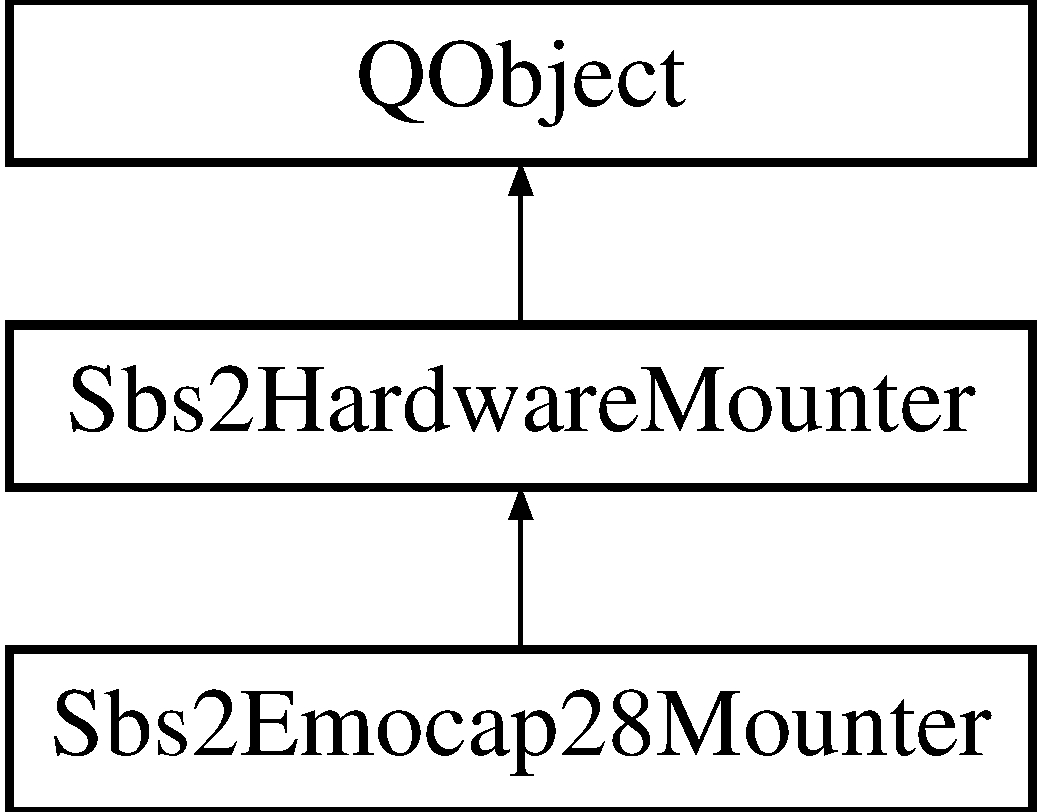
\includegraphics[height=3.000000cm]{classSbs2Emocap28Mounter}
\end{center}
\end{figure}
\subsection*{Public Slots}
\begin{DoxyCompactItemize}
\item 
void \hyperlink{classSbs2Emocap28Mounter_ac2b7d1c8782d36542a0ad05a0c79cf47}{start} ()
\item 
void \hyperlink{classSbs2Emocap28Mounter_af7257b300b705f53d249453ba3fe592f}{stop} ()
\item 
void \hyperlink{classSbs2Emocap28Mounter_a13242b6aa959934acf359f48690c0e8f}{invalidate} ()
\end{DoxyCompactItemize}
\subsection*{Public Member Functions}
\begin{DoxyCompactItemize}
\item 
\hyperlink{classSbs2Emocap28Mounter_aff080ed4f71f6b95c311c5200b04b7ff}{$\sim$\-Sbs2\-Emocap28\-Mounter} ()
\end{DoxyCompactItemize}
\subsection*{Static Public Member Functions}
\begin{DoxyCompactItemize}
\item 
static \hyperlink{classSbs2Emocap28Mounter}{Sbs2\-Emocap28\-Mounter} $\ast$ \hyperlink{classSbs2Emocap28Mounter_ab86f604bf4b29cd4cc1acdcbe91354f0}{New} (Q\-Object $\ast$parent=0)
\end{DoxyCompactItemize}
\subsection*{Additional Inherited Members}


\subsection{Detailed Description}
Smartphone Brain Scanner 2 License Agreement (M\-I\-T License)

Copyright (c) 2012 Arkadiusz Stopczynski, Jakob Eg Larsen, Carsten Stahlhut, Michael Kai Petersen, Lars Kai Hansen. Technical University of Denmark, \hyperlink{namespaceDTU}{D\-T\-U} Informatics, Cognitive Systems Section. \href{http://code.google.com/p/smartphonebrainscanner2}{\tt http\-://code.\-google.\-com/p/smartphonebrainscanner2}

Permission is hereby granted, free of charge, to any person obtaining a copy of this software and associated documentation files (the \char`\"{}\-Software\char`\"{}), to deal in the Software without restriction, including without limitation the rights to use, copy, modify, merge, publish, distribute, sublicense, and/or sell copies of the Software, and to permit persons to whom the Software is furnished to do so, subject to the following conditions\-:

The above copyright notice and this permission notice shall be included in all copies or substantial portions of the Software.

T\-H\-E S\-O\-F\-T\-W\-A\-R\-E I\-S P\-R\-O\-V\-I\-D\-E\-D \char`\"{}\-A\-S I\-S\char`\"{}, W\-I\-T\-H\-O\-U\-T W\-A\-R\-R\-A\-N\-T\-Y O\-F A\-N\-Y K\-I\-N\-D, E\-X\-P\-R\-E\-S\-S O\-R I\-M\-P\-L\-I\-E\-D, I\-N\-C\-L\-U\-D\-I\-N\-G B\-U\-T N\-O\-T L\-I\-M\-I\-T\-E\-D T\-O T\-H\-E W\-A\-R\-R\-A\-N\-T\-I\-E\-S O\-F M\-E\-R\-C\-H\-A\-N\-T\-A\-B\-I\-L\-I\-T\-Y, F\-I\-T\-N\-E\-S\-S F\-O\-R A P\-A\-R\-T\-I\-C\-U\-L\-A\-R P\-U\-R\-P\-O\-S\-E A\-N\-D N\-O\-N\-I\-N\-F\-R\-I\-N\-G\-E\-M\-E\-N\-T. I\-N N\-O E\-V\-E\-N\-T S\-H\-A\-L\-L T\-H\-E A\-U\-T\-H\-O\-R\-S O\-R C\-O\-P\-Y\-R\-I\-G\-H\-T H\-O\-L\-D\-E\-R\-S B\-E L\-I\-A\-B\-L\-E F\-O\-R A\-N\-Y C\-L\-A\-I\-M, D\-A\-M\-A\-G\-E\-S O\-R O\-T\-H\-E\-R L\-I\-A\-B\-I\-L\-I\-T\-Y, W\-H\-E\-T\-H\-E\-R I\-N A\-N A\-C\-T\-I\-O\-N O\-F C\-O\-N\-T\-R\-A\-C\-T, T\-O\-R\-T O\-R O\-T\-H\-E\-R\-W\-I\-S\-E, A\-R\-I\-S\-I\-N\-G F\-R\-O\-M, O\-U\-T O\-F O\-R I\-N C\-O\-N\-N\-E\-C\-T\-I\-O\-N W\-I\-T\-H T\-H\-E S\-O\-F\-T\-W\-A\-R\-E O\-R T\-H\-E U\-S\-E O\-R O\-T\-H\-E\-R D\-E\-A\-L\-I\-N\-G\-S I\-N T\-H\-E S\-O\-F\-T\-W\-A\-R\-E.\-On O\-S\-X we use hidapi to access raw data. 

\subsection{Constructor \& Destructor Documentation}
\hypertarget{classSbs2Emocap28Mounter_aff080ed4f71f6b95c311c5200b04b7ff}{\index{Sbs2\-Emocap28\-Mounter@{Sbs2\-Emocap28\-Mounter}!$\sim$\-Sbs2\-Emocap28\-Mounter@{$\sim$\-Sbs2\-Emocap28\-Mounter}}
\index{$\sim$\-Sbs2\-Emocap28\-Mounter@{$\sim$\-Sbs2\-Emocap28\-Mounter}!Sbs2Emocap28Mounter@{Sbs2\-Emocap28\-Mounter}}
\subsubsection[{$\sim$\-Sbs2\-Emocap28\-Mounter}]{\setlength{\rightskip}{0pt plus 5cm}Sbs2\-Emocap28\-Mounter\-::$\sim$\-Sbs2\-Emocap28\-Mounter (
\begin{DoxyParamCaption}
{}
\end{DoxyParamCaption}
)}}\label{classSbs2Emocap28Mounter_aff080ed4f71f6b95c311c5200b04b7ff}


\subsection{Member Function Documentation}
\hypertarget{classSbs2Emocap28Mounter_a13242b6aa959934acf359f48690c0e8f}{\index{Sbs2\-Emocap28\-Mounter@{Sbs2\-Emocap28\-Mounter}!invalidate@{invalidate}}
\index{invalidate@{invalidate}!Sbs2Emocap28Mounter@{Sbs2\-Emocap28\-Mounter}}
\subsubsection[{invalidate}]{\setlength{\rightskip}{0pt plus 5cm}void Sbs2\-Emocap28\-Mounter\-::invalidate (
\begin{DoxyParamCaption}
{}
\end{DoxyParamCaption}
)\hspace{0.3cm}{\ttfamily [slot]}}}\label{classSbs2Emocap28Mounter_a13242b6aa959934acf359f48690c0e8f}
\hypertarget{classSbs2Emocap28Mounter_ab86f604bf4b29cd4cc1acdcbe91354f0}{\index{Sbs2\-Emocap28\-Mounter@{Sbs2\-Emocap28\-Mounter}!New@{New}}
\index{New@{New}!Sbs2Emocap28Mounter@{Sbs2\-Emocap28\-Mounter}}
\subsubsection[{New}]{\setlength{\rightskip}{0pt plus 5cm}{\bf Sbs2\-Emocap28\-Mounter} $\ast$ Sbs2\-Emocap28\-Mounter\-::\-New (
\begin{DoxyParamCaption}
\item[{Q\-Object $\ast$}]{parent = {\ttfamily 0}}
\end{DoxyParamCaption}
)\hspace{0.3cm}{\ttfamily [static]}}}\label{classSbs2Emocap28Mounter_ab86f604bf4b29cd4cc1acdcbe91354f0}
\hypertarget{classSbs2Emocap28Mounter_ac2b7d1c8782d36542a0ad05a0c79cf47}{\index{Sbs2\-Emocap28\-Mounter@{Sbs2\-Emocap28\-Mounter}!start@{start}}
\index{start@{start}!Sbs2Emocap28Mounter@{Sbs2\-Emocap28\-Mounter}}
\subsubsection[{start}]{\setlength{\rightskip}{0pt plus 5cm}void Sbs2\-Emocap28\-Mounter\-::start (
\begin{DoxyParamCaption}
{}
\end{DoxyParamCaption}
)\hspace{0.3cm}{\ttfamily [slot]}}}\label{classSbs2Emocap28Mounter_ac2b7d1c8782d36542a0ad05a0c79cf47}
\hypertarget{classSbs2Emocap28Mounter_af7257b300b705f53d249453ba3fe592f}{\index{Sbs2\-Emocap28\-Mounter@{Sbs2\-Emocap28\-Mounter}!stop@{stop}}
\index{stop@{stop}!Sbs2Emocap28Mounter@{Sbs2\-Emocap28\-Mounter}}
\subsubsection[{stop}]{\setlength{\rightskip}{0pt plus 5cm}void Sbs2\-Emocap28\-Mounter\-::stop (
\begin{DoxyParamCaption}
{}
\end{DoxyParamCaption}
)\hspace{0.3cm}{\ttfamily [slot]}}}\label{classSbs2Emocap28Mounter_af7257b300b705f53d249453ba3fe592f}


The documentation for this class was generated from the following files\-:\begin{DoxyCompactItemize}
\item 
/media/philipjhj/\-Data/\-One\-Drive/\-Studie/\-Studenterprogrammør/\-S\-B\-S3/smartphonebrainscanner2-\/core/src/hardware/emocap28/\hyperlink{sbs2emocap28mounter_8h}{sbs2emocap28mounter.\-h}\item 
/media/philipjhj/\-Data/\-One\-Drive/\-Studie/\-Studenterprogrammør/\-S\-B\-S3/smartphonebrainscanner2-\/core/src/hardware/emocap28/\hyperlink{sbs2emocap28mounter_8cpp}{sbs2emocap28mounter.\-cpp}\end{DoxyCompactItemize}

\hypertarget{classSbs2Emocap28Packet}{\section{Sbs2\-Emocap28\-Packet Class Reference}
\label{classSbs2Emocap28Packet}\index{Sbs2\-Emocap28\-Packet@{Sbs2\-Emocap28\-Packet}}
}


{\ttfamily \#include $<$sbs2emocap28packet.\-h$>$}

Inheritance diagram for Sbs2\-Emocap28\-Packet\-:\begin{figure}[H]
\begin{center}
\leavevmode
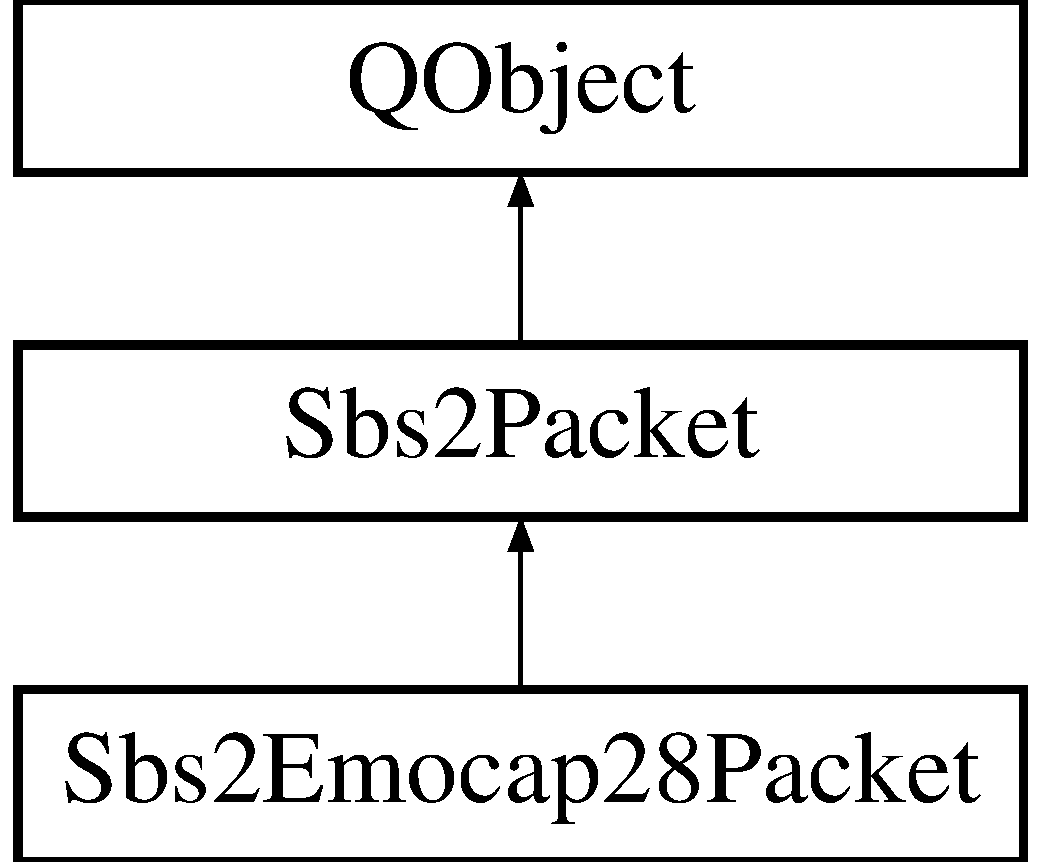
\includegraphics[height=3.000000cm]{classSbs2Emocap28Packet}
\end{center}
\end{figure}
\subsection*{Public Member Functions}
\begin{DoxyCompactItemize}
\item 
\hyperlink{classSbs2Emocap28Packet_a9cdf024eb45f98a684a769546ce6c0cc}{Sbs2\-Emocap28\-Packet} (Q\-Object $\ast$parent)
\item 
void \hyperlink{classSbs2Emocap28Packet_a5fe0695a677da249df1226c310926716}{update} (char $\ast$data)
\begin{DoxyCompactList}\small\item\em Method for updating data in the packet. To avoid continuous creation and destruction of objects, certain number of empty packets is constructed in initialization and then updated with wrap-\/around. Packets should see the raw data delieverd by \hyperlink{classSbs2DataReader}{Sbs2\-Data\-Reader} and form themselves. \end{DoxyCompactList}\item 
void \hyperlink{classSbs2Emocap28Packet_ab8e2defdaf6cdf3586e5fab59359d66d}{update} (char $\ast$data1, char $\ast$data2)
\item 
int \hyperlink{classSbs2Emocap28Packet_a4b3a6363a12c66a81a939f5c5e1e3c9a}{get\-Counter} (char $\ast$data)
\item 
int \hyperlink{classSbs2Emocap28Packet_a5f097181f28c069fbd50d89d821126a0}{get\-Value} (char $\ast$data)
\end{DoxyCompactItemize}
\subsection*{Additional Inherited Members}


\subsection{Detailed Description}
Smartphone Brain Scanner 2 License Agreement (M\-I\-T License)

Copyright (c) 2012 Arkadiusz Stopczynski, Jakob Eg Larsen, Carsten Stahlhut, Michael Kai Petersen, Lars Kai Hansen. Technical University of Denmark, \hyperlink{namespaceDTU}{D\-T\-U} Informatics, Cognitive Systems Section. \href{http://code.google.com/p/smartphonebrainscanner2}{\tt http\-://code.\-google.\-com/p/smartphonebrainscanner2}

Permission is hereby granted, free of charge, to any person obtaining a copy of this software and associated documentation files (the \char`\"{}\-Software\char`\"{}), to deal in the Software without restriction, including without limitation the rights to use, copy, modify, merge, publish, distribute, sublicense, and/or sell copies of the Software, and to permit persons to whom the Software is furnished to do so, subject to the following conditions\-:

The above copyright notice and this permission notice shall be included in all copies or substantial portions of the Software.

T\-H\-E S\-O\-F\-T\-W\-A\-R\-E I\-S P\-R\-O\-V\-I\-D\-E\-D \char`\"{}\-A\-S I\-S\char`\"{}, W\-I\-T\-H\-O\-U\-T W\-A\-R\-R\-A\-N\-T\-Y O\-F A\-N\-Y K\-I\-N\-D, E\-X\-P\-R\-E\-S\-S O\-R I\-M\-P\-L\-I\-E\-D, I\-N\-C\-L\-U\-D\-I\-N\-G B\-U\-T N\-O\-T L\-I\-M\-I\-T\-E\-D T\-O T\-H\-E W\-A\-R\-R\-A\-N\-T\-I\-E\-S O\-F M\-E\-R\-C\-H\-A\-N\-T\-A\-B\-I\-L\-I\-T\-Y, F\-I\-T\-N\-E\-S\-S F\-O\-R A P\-A\-R\-T\-I\-C\-U\-L\-A\-R P\-U\-R\-P\-O\-S\-E A\-N\-D N\-O\-N\-I\-N\-F\-R\-I\-N\-G\-E\-M\-E\-N\-T. I\-N N\-O E\-V\-E\-N\-T S\-H\-A\-L\-L T\-H\-E A\-U\-T\-H\-O\-R\-S O\-R C\-O\-P\-Y\-R\-I\-G\-H\-T H\-O\-L\-D\-E\-R\-S B\-E L\-I\-A\-B\-L\-E F\-O\-R A\-N\-Y C\-L\-A\-I\-M, D\-A\-M\-A\-G\-E\-S O\-R O\-T\-H\-E\-R L\-I\-A\-B\-I\-L\-I\-T\-Y, W\-H\-E\-T\-H\-E\-R I\-N A\-N A\-C\-T\-I\-O\-N O\-F C\-O\-N\-T\-R\-A\-C\-T, T\-O\-R\-T O\-R O\-T\-H\-E\-R\-W\-I\-S\-E, A\-R\-I\-S\-I\-N\-G F\-R\-O\-M, O\-U\-T O\-F O\-R I\-N C\-O\-N\-N\-E\-C\-T\-I\-O\-N W\-I\-T\-H T\-H\-E S\-O\-F\-T\-W\-A\-R\-E O\-R T\-H\-E U\-S\-E O\-R O\-T\-H\-E\-R D\-E\-A\-L\-I\-N\-G\-S I\-N T\-H\-E S\-O\-F\-T\-W\-A\-R\-E. 

\subsection{Constructor \& Destructor Documentation}
\hypertarget{classSbs2Emocap28Packet_a9cdf024eb45f98a684a769546ce6c0cc}{\index{Sbs2\-Emocap28\-Packet@{Sbs2\-Emocap28\-Packet}!Sbs2\-Emocap28\-Packet@{Sbs2\-Emocap28\-Packet}}
\index{Sbs2\-Emocap28\-Packet@{Sbs2\-Emocap28\-Packet}!Sbs2Emocap28Packet@{Sbs2\-Emocap28\-Packet}}
\subsubsection[{Sbs2\-Emocap28\-Packet}]{\setlength{\rightskip}{0pt plus 5cm}Sbs2\-Emocap28\-Packet\-::\-Sbs2\-Emocap28\-Packet (
\begin{DoxyParamCaption}
\item[{Q\-Object $\ast$}]{parent}
\end{DoxyParamCaption}
)}}\label{classSbs2Emocap28Packet_a9cdf024eb45f98a684a769546ce6c0cc}


\subsection{Member Function Documentation}
\hypertarget{classSbs2Emocap28Packet_a4b3a6363a12c66a81a939f5c5e1e3c9a}{\index{Sbs2\-Emocap28\-Packet@{Sbs2\-Emocap28\-Packet}!get\-Counter@{get\-Counter}}
\index{get\-Counter@{get\-Counter}!Sbs2Emocap28Packet@{Sbs2\-Emocap28\-Packet}}
\subsubsection[{get\-Counter}]{\setlength{\rightskip}{0pt plus 5cm}int Sbs2\-Emocap28\-Packet\-::get\-Counter (
\begin{DoxyParamCaption}
\item[{char $\ast$}]{data}
\end{DoxyParamCaption}
)}}\label{classSbs2Emocap28Packet_a4b3a6363a12c66a81a939f5c5e1e3c9a}
\hypertarget{classSbs2Emocap28Packet_a5f097181f28c069fbd50d89d821126a0}{\index{Sbs2\-Emocap28\-Packet@{Sbs2\-Emocap28\-Packet}!get\-Value@{get\-Value}}
\index{get\-Value@{get\-Value}!Sbs2Emocap28Packet@{Sbs2\-Emocap28\-Packet}}
\subsubsection[{get\-Value}]{\setlength{\rightskip}{0pt plus 5cm}int Sbs2\-Emocap28\-Packet\-::get\-Value (
\begin{DoxyParamCaption}
\item[{char $\ast$}]{data}
\end{DoxyParamCaption}
)}}\label{classSbs2Emocap28Packet_a5f097181f28c069fbd50d89d821126a0}
\hypertarget{classSbs2Emocap28Packet_a5fe0695a677da249df1226c310926716}{\index{Sbs2\-Emocap28\-Packet@{Sbs2\-Emocap28\-Packet}!update@{update}}
\index{update@{update}!Sbs2Emocap28Packet@{Sbs2\-Emocap28\-Packet}}
\subsubsection[{update}]{\setlength{\rightskip}{0pt plus 5cm}void Sbs2\-Emocap28\-Packet\-::update (
\begin{DoxyParamCaption}
\item[{char $\ast$}]{data}
\end{DoxyParamCaption}
)\hspace{0.3cm}{\ttfamily [virtual]}}}\label{classSbs2Emocap28Packet_a5fe0695a677da249df1226c310926716}


Method for updating data in the packet. To avoid continuous creation and destruction of objects, certain number of empty packets is constructed in initialization and then updated with wrap-\/around. Packets should see the raw data delieverd by \hyperlink{classSbs2DataReader}{Sbs2\-Data\-Reader} and form themselves. 


\begin{DoxyParams}{Parameters}
{\em data} & Pointer to raw data. \\
\hline
\end{DoxyParams}


Reimplemented from \hyperlink{classSbs2Packet_a8b80c76000ceead51e9278c833bb56ae}{Sbs2\-Packet}.

\hypertarget{classSbs2Emocap28Packet_ab8e2defdaf6cdf3586e5fab59359d66d}{\index{Sbs2\-Emocap28\-Packet@{Sbs2\-Emocap28\-Packet}!update@{update}}
\index{update@{update}!Sbs2Emocap28Packet@{Sbs2\-Emocap28\-Packet}}
\subsubsection[{update}]{\setlength{\rightskip}{0pt plus 5cm}void Sbs2\-Emocap28\-Packet\-::update (
\begin{DoxyParamCaption}
\item[{char $\ast$}]{data1, }
\item[{char $\ast$}]{data2}
\end{DoxyParamCaption}
)}}\label{classSbs2Emocap28Packet_ab8e2defdaf6cdf3586e5fab59359d66d}


The documentation for this class was generated from the following files\-:\begin{DoxyCompactItemize}
\item 
/media/philipjhj/\-Data/\-One\-Drive/\-Studie/\-Studenterprogrammør/\-S\-B\-S3/smartphonebrainscanner2-\/core/src/hardware/emocap28/\hyperlink{sbs2emocap28packet_8h}{sbs2emocap28packet.\-h}\item 
/media/philipjhj/\-Data/\-One\-Drive/\-Studie/\-Studenterprogrammør/\-S\-B\-S3/smartphonebrainscanner2-\/core/src/hardware/emocap28/\hyperlink{sbs2emocap28packet_8cpp}{sbs2emocap28packet.\-cpp}\end{DoxyCompactItemize}

\hypertarget{classSbs2EmocapDataReader}{\section{Sbs2\-Emocap\-Data\-Reader Class Reference}
\label{classSbs2EmocapDataReader}\index{Sbs2\-Emocap\-Data\-Reader@{Sbs2\-Emocap\-Data\-Reader}}
}


{\ttfamily \#include $<$sbs2emocapdatareader.\-h$>$}

Inheritance diagram for Sbs2\-Emocap\-Data\-Reader\-:\begin{figure}[H]
\begin{center}
\leavevmode
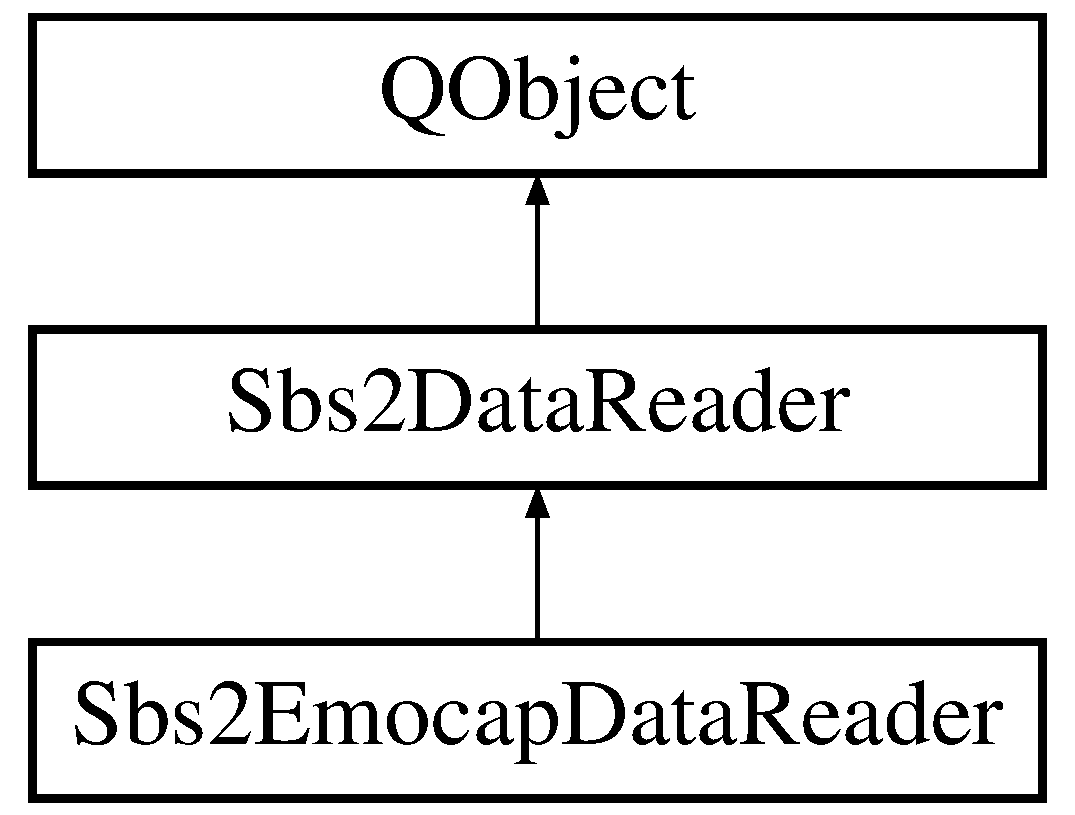
\includegraphics[height=3.000000cm]{classSbs2EmocapDataReader}
\end{center}
\end{figure}
\subsection*{Public Slots}
\begin{DoxyCompactItemize}
\item 
void \hyperlink{classSbs2EmocapDataReader_ab47ef67e7956bd710aedd233f127498b}{device\-Found} (Q\-Map$<$ Q\-String, Q\-Variant $>$ params)
\item 
void \hyperlink{classSbs2EmocapDataReader_a799188dcf1f2499e592bf3bf70eef282}{device\-Lost} ()
\item 
void \hyperlink{classSbs2EmocapDataReader_a327f5896de2f2c9bd995db3b921b7004}{about\-To\-Quit} ()
\item 
void \hyperlink{classSbs2EmocapDataReader_a2afdbee6829e11aaf34b250c87503323}{udp\-Data\-Received} (Q\-Vector$<$ char $\ast$ $>$ $\ast$data, int counter)
\item 
void \hyperlink{classSbs2EmocapDataReader_a41a4b861c75eacdc2ff6dbace6ddd4fd}{udp\-Data\-Received} (Q\-Udp\-Socket $\ast$raw\-Data\-Udp\-Input\-Socket)
\item 
void \hyperlink{classSbs2EmocapDataReader_a6923ac53e782bc04a0f346836a237b01}{turn\-Receive\-Udp\-Data\-On} (Q\-String address, int port)
\item 
void \hyperlink{classSbs2EmocapDataReader_af747a8d7ecef45e0502dcd6788f01bcf}{turn\-Receive\-Udp\-Data\-Off} ()
\end{DoxyCompactItemize}
\subsection*{Public Member Functions}
\begin{DoxyCompactItemize}
\item 
\hyperlink{classSbs2EmocapDataReader_a033e577741b84e7bee3be631e7358dda}{$\sim$\-Sbs2\-Emocap\-Data\-Reader} ()
\end{DoxyCompactItemize}
\subsection*{Static Public Member Functions}
\begin{DoxyCompactItemize}
\item 
static \hyperlink{classSbs2EmocapDataReader}{Sbs2\-Emocap\-Data\-Reader} $\ast$ \hyperlink{classSbs2EmocapDataReader_aa5717d7eda59221797a93d71d4086807}{New} (\hyperlink{classSbs2Callback}{Sbs2\-Callback} $\ast$sbs2\-Callback\-\_\-, int read\-Only\-From\-Network\-\_\-=0, Q\-Object $\ast$parent=0)
\end{DoxyCompactItemize}
\subsection*{Additional Inherited Members}


\subsection{Detailed Description}
Smartphone Brain Scanner 2 License Agreement (M\-I\-T License)

Copyright (c) 2012 Arkadiusz Stopczynski, Jakob Eg Larsen, Carsten Stahlhut, Michael Kai Petersen, Lars Kai Hansen. Technical University of Denmark, \hyperlink{namespaceDTU}{D\-T\-U} Informatics, Cognitive Systems Section. \href{http://code.google.com/p/smartphonebrainscanner2}{\tt http\-://code.\-google.\-com/p/smartphonebrainscanner2}

Permission is hereby granted, free of charge, to any person obtaining a copy of this software and associated documentation files (the \char`\"{}\-Software\char`\"{}), to deal in the Software without restriction, including without limitation the rights to use, copy, modify, merge, publish, distribute, sublicense, and/or sell copies of the Software, and to permit persons to whom the Software is furnished to do so, subject to the following conditions\-:

The above copyright notice and this permission notice shall be included in all copies or substantial portions of the Software.

T\-H\-E S\-O\-F\-T\-W\-A\-R\-E I\-S P\-R\-O\-V\-I\-D\-E\-D \char`\"{}\-A\-S I\-S\char`\"{}, W\-I\-T\-H\-O\-U\-T W\-A\-R\-R\-A\-N\-T\-Y O\-F A\-N\-Y K\-I\-N\-D, E\-X\-P\-R\-E\-S\-S O\-R I\-M\-P\-L\-I\-E\-D, I\-N\-C\-L\-U\-D\-I\-N\-G B\-U\-T N\-O\-T L\-I\-M\-I\-T\-E\-D T\-O T\-H\-E W\-A\-R\-R\-A\-N\-T\-I\-E\-S O\-F M\-E\-R\-C\-H\-A\-N\-T\-A\-B\-I\-L\-I\-T\-Y, F\-I\-T\-N\-E\-S\-S F\-O\-R A P\-A\-R\-T\-I\-C\-U\-L\-A\-R P\-U\-R\-P\-O\-S\-E A\-N\-D N\-O\-N\-I\-N\-F\-R\-I\-N\-G\-E\-M\-E\-N\-T. I\-N N\-O E\-V\-E\-N\-T S\-H\-A\-L\-L T\-H\-E A\-U\-T\-H\-O\-R\-S O\-R C\-O\-P\-Y\-R\-I\-G\-H\-T H\-O\-L\-D\-E\-R\-S B\-E L\-I\-A\-B\-L\-E F\-O\-R A\-N\-Y C\-L\-A\-I\-M, D\-A\-M\-A\-G\-E\-S O\-R O\-T\-H\-E\-R L\-I\-A\-B\-I\-L\-I\-T\-Y, W\-H\-E\-T\-H\-E\-R I\-N A\-N A\-C\-T\-I\-O\-N O\-F C\-O\-N\-T\-R\-A\-C\-T, T\-O\-R\-T O\-R O\-T\-H\-E\-R\-W\-I\-S\-E, A\-R\-I\-S\-I\-N\-G F\-R\-O\-M, O\-U\-T O\-F O\-R I\-N C\-O\-N\-N\-E\-C\-T\-I\-O\-N W\-I\-T\-H T\-H\-E S\-O\-F\-T\-W\-A\-R\-E O\-R T\-H\-E U\-S\-E O\-R O\-T\-H\-E\-R D\-E\-A\-L\-I\-N\-G\-S I\-N T\-H\-E S\-O\-F\-T\-W\-A\-R\-E. 

\subsection{Constructor \& Destructor Documentation}
\hypertarget{classSbs2EmocapDataReader_a033e577741b84e7bee3be631e7358dda}{\index{Sbs2\-Emocap\-Data\-Reader@{Sbs2\-Emocap\-Data\-Reader}!$\sim$\-Sbs2\-Emocap\-Data\-Reader@{$\sim$\-Sbs2\-Emocap\-Data\-Reader}}
\index{$\sim$\-Sbs2\-Emocap\-Data\-Reader@{$\sim$\-Sbs2\-Emocap\-Data\-Reader}!Sbs2EmocapDataReader@{Sbs2\-Emocap\-Data\-Reader}}
\subsubsection[{$\sim$\-Sbs2\-Emocap\-Data\-Reader}]{\setlength{\rightskip}{0pt plus 5cm}Sbs2\-Emocap\-Data\-Reader\-::$\sim$\-Sbs2\-Emocap\-Data\-Reader (
\begin{DoxyParamCaption}
{}
\end{DoxyParamCaption}
)}}\label{classSbs2EmocapDataReader_a033e577741b84e7bee3be631e7358dda}


\subsection{Member Function Documentation}
\hypertarget{classSbs2EmocapDataReader_a327f5896de2f2c9bd995db3b921b7004}{\index{Sbs2\-Emocap\-Data\-Reader@{Sbs2\-Emocap\-Data\-Reader}!about\-To\-Quit@{about\-To\-Quit}}
\index{about\-To\-Quit@{about\-To\-Quit}!Sbs2EmocapDataReader@{Sbs2\-Emocap\-Data\-Reader}}
\subsubsection[{about\-To\-Quit}]{\setlength{\rightskip}{0pt plus 5cm}void Sbs2\-Emocap\-Data\-Reader\-::about\-To\-Quit (
\begin{DoxyParamCaption}
{}
\end{DoxyParamCaption}
)\hspace{0.3cm}{\ttfamily [slot]}}}\label{classSbs2EmocapDataReader_a327f5896de2f2c9bd995db3b921b7004}
\hypertarget{classSbs2EmocapDataReader_ab47ef67e7956bd710aedd233f127498b}{\index{Sbs2\-Emocap\-Data\-Reader@{Sbs2\-Emocap\-Data\-Reader}!device\-Found@{device\-Found}}
\index{device\-Found@{device\-Found}!Sbs2EmocapDataReader@{Sbs2\-Emocap\-Data\-Reader}}
\subsubsection[{device\-Found}]{\setlength{\rightskip}{0pt plus 5cm}void Sbs2\-Emocap\-Data\-Reader\-::device\-Found (
\begin{DoxyParamCaption}
\item[{Q\-Map$<$ Q\-String, Q\-Variant $>$}]{params}
\end{DoxyParamCaption}
)\hspace{0.3cm}{\ttfamily [slot]}}}\label{classSbs2EmocapDataReader_ab47ef67e7956bd710aedd233f127498b}
\hypertarget{classSbs2EmocapDataReader_a799188dcf1f2499e592bf3bf70eef282}{\index{Sbs2\-Emocap\-Data\-Reader@{Sbs2\-Emocap\-Data\-Reader}!device\-Lost@{device\-Lost}}
\index{device\-Lost@{device\-Lost}!Sbs2EmocapDataReader@{Sbs2\-Emocap\-Data\-Reader}}
\subsubsection[{device\-Lost}]{\setlength{\rightskip}{0pt plus 5cm}void Sbs2\-Emocap\-Data\-Reader\-::device\-Lost (
\begin{DoxyParamCaption}
{}
\end{DoxyParamCaption}
)\hspace{0.3cm}{\ttfamily [slot]}}}\label{classSbs2EmocapDataReader_a799188dcf1f2499e592bf3bf70eef282}
\hypertarget{classSbs2EmocapDataReader_aa5717d7eda59221797a93d71d4086807}{\index{Sbs2\-Emocap\-Data\-Reader@{Sbs2\-Emocap\-Data\-Reader}!New@{New}}
\index{New@{New}!Sbs2EmocapDataReader@{Sbs2\-Emocap\-Data\-Reader}}
\subsubsection[{New}]{\setlength{\rightskip}{0pt plus 5cm}{\bf Sbs2\-Emocap\-Data\-Reader} $\ast$ Sbs2\-Emocap\-Data\-Reader\-::\-New (
\begin{DoxyParamCaption}
\item[{{\bf Sbs2\-Callback} $\ast$}]{sbs2\-Callback\-\_\-, }
\item[{int}]{read\-Only\-From\-Network\-\_\- = {\ttfamily 0}, }
\item[{Q\-Object $\ast$}]{parent = {\ttfamily 0}}
\end{DoxyParamCaption}
)\hspace{0.3cm}{\ttfamily [static]}}}\label{classSbs2EmocapDataReader_aa5717d7eda59221797a93d71d4086807}
\hypertarget{classSbs2EmocapDataReader_af747a8d7ecef45e0502dcd6788f01bcf}{\index{Sbs2\-Emocap\-Data\-Reader@{Sbs2\-Emocap\-Data\-Reader}!turn\-Receive\-Udp\-Data\-Off@{turn\-Receive\-Udp\-Data\-Off}}
\index{turn\-Receive\-Udp\-Data\-Off@{turn\-Receive\-Udp\-Data\-Off}!Sbs2EmocapDataReader@{Sbs2\-Emocap\-Data\-Reader}}
\subsubsection[{turn\-Receive\-Udp\-Data\-Off}]{\setlength{\rightskip}{0pt plus 5cm}void Sbs2\-Emocap\-Data\-Reader\-::turn\-Receive\-Udp\-Data\-Off (
\begin{DoxyParamCaption}
{}
\end{DoxyParamCaption}
)\hspace{0.3cm}{\ttfamily [slot]}}}\label{classSbs2EmocapDataReader_af747a8d7ecef45e0502dcd6788f01bcf}
\hypertarget{classSbs2EmocapDataReader_a6923ac53e782bc04a0f346836a237b01}{\index{Sbs2\-Emocap\-Data\-Reader@{Sbs2\-Emocap\-Data\-Reader}!turn\-Receive\-Udp\-Data\-On@{turn\-Receive\-Udp\-Data\-On}}
\index{turn\-Receive\-Udp\-Data\-On@{turn\-Receive\-Udp\-Data\-On}!Sbs2EmocapDataReader@{Sbs2\-Emocap\-Data\-Reader}}
\subsubsection[{turn\-Receive\-Udp\-Data\-On}]{\setlength{\rightskip}{0pt plus 5cm}void Sbs2\-Emocap\-Data\-Reader\-::turn\-Receive\-Udp\-Data\-On (
\begin{DoxyParamCaption}
\item[{Q\-String}]{address, }
\item[{int}]{port}
\end{DoxyParamCaption}
)\hspace{0.3cm}{\ttfamily [slot]}}}\label{classSbs2EmocapDataReader_a6923ac53e782bc04a0f346836a237b01}
\hypertarget{classSbs2EmocapDataReader_a2afdbee6829e11aaf34b250c87503323}{\index{Sbs2\-Emocap\-Data\-Reader@{Sbs2\-Emocap\-Data\-Reader}!udp\-Data\-Received@{udp\-Data\-Received}}
\index{udp\-Data\-Received@{udp\-Data\-Received}!Sbs2EmocapDataReader@{Sbs2\-Emocap\-Data\-Reader}}
\subsubsection[{udp\-Data\-Received}]{\setlength{\rightskip}{0pt plus 5cm}void Sbs2\-Emocap\-Data\-Reader\-::udp\-Data\-Received (
\begin{DoxyParamCaption}
\item[{Q\-Vector$<$ char $\ast$ $>$ $\ast$}]{data, }
\item[{int}]{counter}
\end{DoxyParamCaption}
)\hspace{0.3cm}{\ttfamily [slot]}}}\label{classSbs2EmocapDataReader_a2afdbee6829e11aaf34b250c87503323}
\hypertarget{classSbs2EmocapDataReader_a41a4b861c75eacdc2ff6dbace6ddd4fd}{\index{Sbs2\-Emocap\-Data\-Reader@{Sbs2\-Emocap\-Data\-Reader}!udp\-Data\-Received@{udp\-Data\-Received}}
\index{udp\-Data\-Received@{udp\-Data\-Received}!Sbs2EmocapDataReader@{Sbs2\-Emocap\-Data\-Reader}}
\subsubsection[{udp\-Data\-Received}]{\setlength{\rightskip}{0pt plus 5cm}void Sbs2\-Emocap\-Data\-Reader\-::udp\-Data\-Received (
\begin{DoxyParamCaption}
\item[{Q\-Udp\-Socket $\ast$}]{raw\-Data\-Udp\-Input\-Socket}
\end{DoxyParamCaption}
)\hspace{0.3cm}{\ttfamily [slot]}}}\label{classSbs2EmocapDataReader_a41a4b861c75eacdc2ff6dbace6ddd4fd}


The documentation for this class was generated from the following files\-:\begin{DoxyCompactItemize}
\item 
/media/philipjhj/\-Data/\-One\-Drive/\-Studie/\-Studenterprogrammør/\-S\-B\-S3/smartphonebrainscanner2-\/core/src/hardware/emocap/\hyperlink{sbs2emocapdatareader_8h}{sbs2emocapdatareader.\-h}\item 
/media/philipjhj/\-Data/\-One\-Drive/\-Studie/\-Studenterprogrammør/\-S\-B\-S3/smartphonebrainscanner2-\/core/src/hardware/emocap/\hyperlink{sbs2emocapdatareader_8cpp}{sbs2emocapdatareader.\-cpp}\end{DoxyCompactItemize}

\hypertarget{classSbs2EmocapMounter}{\section{Sbs2\-Emocap\-Mounter Class Reference}
\label{classSbs2EmocapMounter}\index{Sbs2\-Emocap\-Mounter@{Sbs2\-Emocap\-Mounter}}
}


{\ttfamily \#include $<$sbs2emocapmounter.\-h$>$}

Inheritance diagram for Sbs2\-Emocap\-Mounter\-:\begin{figure}[H]
\begin{center}
\leavevmode
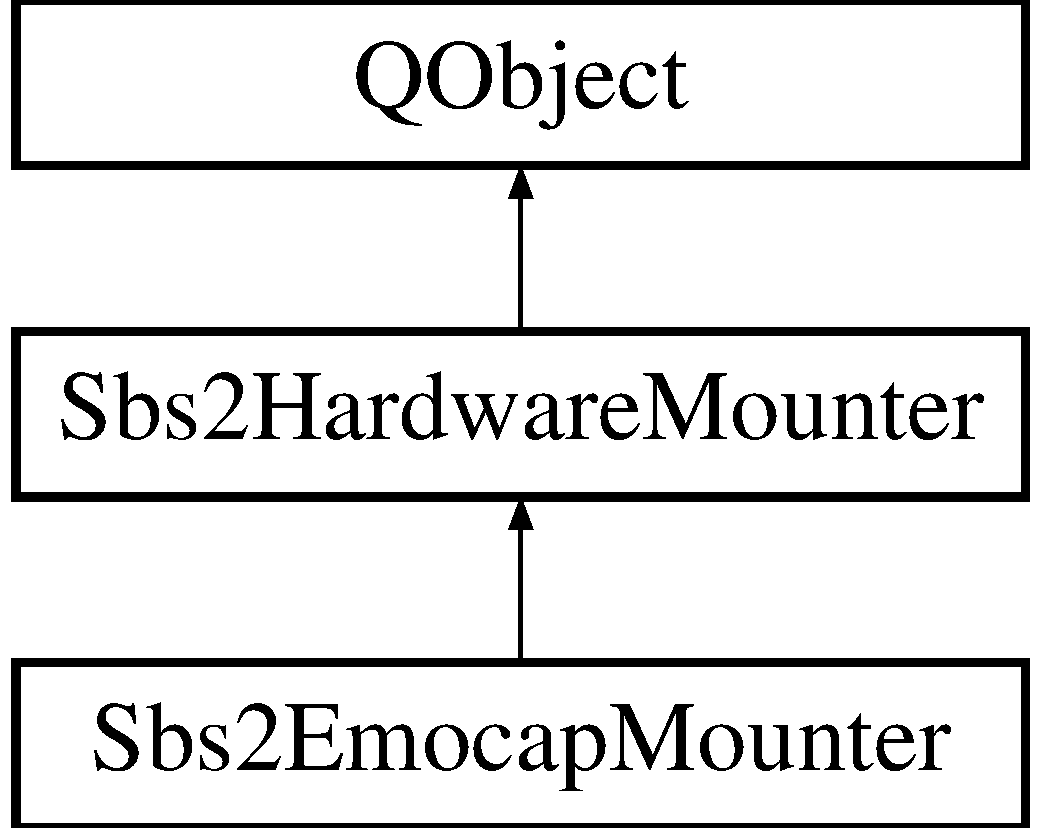
\includegraphics[height=3.000000cm]{classSbs2EmocapMounter}
\end{center}
\end{figure}
\subsection*{Public Slots}
\begin{DoxyCompactItemize}
\item 
void \hyperlink{classSbs2EmocapMounter_a25805c484788e484bdac53a806c822eb}{start} ()
\item 
void \hyperlink{classSbs2EmocapMounter_a6ad15728a9361481d85480a9ec7fa8dd}{stop} ()
\item 
void \hyperlink{classSbs2EmocapMounter_a77a3a401dfa47baf5f7d0e70095c7072}{invalidate} ()
\end{DoxyCompactItemize}
\subsection*{Public Member Functions}
\begin{DoxyCompactItemize}
\item 
\hyperlink{classSbs2EmocapMounter_a1df4f11a64da9aa21ba890c8991b4912}{$\sim$\-Sbs2\-Emocap\-Mounter} ()
\end{DoxyCompactItemize}
\subsection*{Static Public Member Functions}
\begin{DoxyCompactItemize}
\item 
static \hyperlink{classSbs2EmocapMounter}{Sbs2\-Emocap\-Mounter} $\ast$ \hyperlink{classSbs2EmocapMounter_a356acdbf5ccaab6ff730b29c4e25a260}{New} (Q\-Object $\ast$parent=0)
\end{DoxyCompactItemize}
\subsection*{Additional Inherited Members}


\subsection{Detailed Description}
Smartphone Brain Scanner 2 License Agreement (M\-I\-T License)

Copyright (c) 2012 Arkadiusz Stopczynski, Jakob Eg Larsen, Carsten Stahlhut, Michael Kai Petersen, Lars Kai Hansen. Technical University of Denmark, \hyperlink{namespaceDTU}{D\-T\-U} Informatics, Cognitive Systems Section. \href{http://code.google.com/p/smartphonebrainscanner2}{\tt http\-://code.\-google.\-com/p/smartphonebrainscanner2}

Permission is hereby granted, free of charge, to any person obtaining a copy of this software and associated documentation files (the \char`\"{}\-Software\char`\"{}), to deal in the Software without restriction, including without limitation the rights to use, copy, modify, merge, publish, distribute, sublicense, and/or sell copies of the Software, and to permit persons to whom the Software is furnished to do so, subject to the following conditions\-:

The above copyright notice and this permission notice shall be included in all copies or substantial portions of the Software.

T\-H\-E S\-O\-F\-T\-W\-A\-R\-E I\-S P\-R\-O\-V\-I\-D\-E\-D \char`\"{}\-A\-S I\-S\char`\"{}, W\-I\-T\-H\-O\-U\-T W\-A\-R\-R\-A\-N\-T\-Y O\-F A\-N\-Y K\-I\-N\-D, E\-X\-P\-R\-E\-S\-S O\-R I\-M\-P\-L\-I\-E\-D, I\-N\-C\-L\-U\-D\-I\-N\-G B\-U\-T N\-O\-T L\-I\-M\-I\-T\-E\-D T\-O T\-H\-E W\-A\-R\-R\-A\-N\-T\-I\-E\-S O\-F M\-E\-R\-C\-H\-A\-N\-T\-A\-B\-I\-L\-I\-T\-Y, F\-I\-T\-N\-E\-S\-S F\-O\-R A P\-A\-R\-T\-I\-C\-U\-L\-A\-R P\-U\-R\-P\-O\-S\-E A\-N\-D N\-O\-N\-I\-N\-F\-R\-I\-N\-G\-E\-M\-E\-N\-T. I\-N N\-O E\-V\-E\-N\-T S\-H\-A\-L\-L T\-H\-E A\-U\-T\-H\-O\-R\-S O\-R C\-O\-P\-Y\-R\-I\-G\-H\-T H\-O\-L\-D\-E\-R\-S B\-E L\-I\-A\-B\-L\-E F\-O\-R A\-N\-Y C\-L\-A\-I\-M, D\-A\-M\-A\-G\-E\-S O\-R O\-T\-H\-E\-R L\-I\-A\-B\-I\-L\-I\-T\-Y, W\-H\-E\-T\-H\-E\-R I\-N A\-N A\-C\-T\-I\-O\-N O\-F C\-O\-N\-T\-R\-A\-C\-T, T\-O\-R\-T O\-R O\-T\-H\-E\-R\-W\-I\-S\-E, A\-R\-I\-S\-I\-N\-G F\-R\-O\-M, O\-U\-T O\-F O\-R I\-N C\-O\-N\-N\-E\-C\-T\-I\-O\-N W\-I\-T\-H T\-H\-E S\-O\-F\-T\-W\-A\-R\-E O\-R T\-H\-E U\-S\-E O\-R O\-T\-H\-E\-R D\-E\-A\-L\-I\-N\-G\-S I\-N T\-H\-E S\-O\-F\-T\-W\-A\-R\-E.\-On O\-S\-X we use hidapi to access raw data. 

\subsection{Constructor \& Destructor Documentation}
\hypertarget{classSbs2EmocapMounter_a1df4f11a64da9aa21ba890c8991b4912}{\index{Sbs2\-Emocap\-Mounter@{Sbs2\-Emocap\-Mounter}!$\sim$\-Sbs2\-Emocap\-Mounter@{$\sim$\-Sbs2\-Emocap\-Mounter}}
\index{$\sim$\-Sbs2\-Emocap\-Mounter@{$\sim$\-Sbs2\-Emocap\-Mounter}!Sbs2EmocapMounter@{Sbs2\-Emocap\-Mounter}}
\subsubsection[{$\sim$\-Sbs2\-Emocap\-Mounter}]{\setlength{\rightskip}{0pt plus 5cm}Sbs2\-Emocap\-Mounter\-::$\sim$\-Sbs2\-Emocap\-Mounter (
\begin{DoxyParamCaption}
{}
\end{DoxyParamCaption}
)}}\label{classSbs2EmocapMounter_a1df4f11a64da9aa21ba890c8991b4912}


\subsection{Member Function Documentation}
\hypertarget{classSbs2EmocapMounter_a77a3a401dfa47baf5f7d0e70095c7072}{\index{Sbs2\-Emocap\-Mounter@{Sbs2\-Emocap\-Mounter}!invalidate@{invalidate}}
\index{invalidate@{invalidate}!Sbs2EmocapMounter@{Sbs2\-Emocap\-Mounter}}
\subsubsection[{invalidate}]{\setlength{\rightskip}{0pt plus 5cm}void Sbs2\-Emocap\-Mounter\-::invalidate (
\begin{DoxyParamCaption}
{}
\end{DoxyParamCaption}
)\hspace{0.3cm}{\ttfamily [slot]}}}\label{classSbs2EmocapMounter_a77a3a401dfa47baf5f7d0e70095c7072}
\hypertarget{classSbs2EmocapMounter_a356acdbf5ccaab6ff730b29c4e25a260}{\index{Sbs2\-Emocap\-Mounter@{Sbs2\-Emocap\-Mounter}!New@{New}}
\index{New@{New}!Sbs2EmocapMounter@{Sbs2\-Emocap\-Mounter}}
\subsubsection[{New}]{\setlength{\rightskip}{0pt plus 5cm}{\bf Sbs2\-Emocap\-Mounter} $\ast$ Sbs2\-Emocap\-Mounter\-::\-New (
\begin{DoxyParamCaption}
\item[{Q\-Object $\ast$}]{parent = {\ttfamily 0}}
\end{DoxyParamCaption}
)\hspace{0.3cm}{\ttfamily [static]}}}\label{classSbs2EmocapMounter_a356acdbf5ccaab6ff730b29c4e25a260}
\hypertarget{classSbs2EmocapMounter_a25805c484788e484bdac53a806c822eb}{\index{Sbs2\-Emocap\-Mounter@{Sbs2\-Emocap\-Mounter}!start@{start}}
\index{start@{start}!Sbs2EmocapMounter@{Sbs2\-Emocap\-Mounter}}
\subsubsection[{start}]{\setlength{\rightskip}{0pt plus 5cm}void Sbs2\-Emocap\-Mounter\-::start (
\begin{DoxyParamCaption}
{}
\end{DoxyParamCaption}
)\hspace{0.3cm}{\ttfamily [slot]}}}\label{classSbs2EmocapMounter_a25805c484788e484bdac53a806c822eb}
\hypertarget{classSbs2EmocapMounter_a6ad15728a9361481d85480a9ec7fa8dd}{\index{Sbs2\-Emocap\-Mounter@{Sbs2\-Emocap\-Mounter}!stop@{stop}}
\index{stop@{stop}!Sbs2EmocapMounter@{Sbs2\-Emocap\-Mounter}}
\subsubsection[{stop}]{\setlength{\rightskip}{0pt plus 5cm}void Sbs2\-Emocap\-Mounter\-::stop (
\begin{DoxyParamCaption}
{}
\end{DoxyParamCaption}
)\hspace{0.3cm}{\ttfamily [slot]}}}\label{classSbs2EmocapMounter_a6ad15728a9361481d85480a9ec7fa8dd}


The documentation for this class was generated from the following files\-:\begin{DoxyCompactItemize}
\item 
/media/philipjhj/\-Data/\-One\-Drive/\-Studie/\-Studenterprogrammør/\-S\-B\-S3/smartphonebrainscanner2-\/core/src/hardware/emocap/\hyperlink{sbs2emocapmounter_8h}{sbs2emocapmounter.\-h}\item 
/media/philipjhj/\-Data/\-One\-Drive/\-Studie/\-Studenterprogrammør/\-S\-B\-S3/smartphonebrainscanner2-\/core/src/hardware/emocap/\hyperlink{sbs2emocapmounter_8cpp}{sbs2emocapmounter.\-cpp}\end{DoxyCompactItemize}

\hypertarget{classSbs2EmocapPacket}{\section{Sbs2\-Emocap\-Packet Class Reference}
\label{classSbs2EmocapPacket}\index{Sbs2\-Emocap\-Packet@{Sbs2\-Emocap\-Packet}}
}


{\ttfamily \#include $<$sbs2emocappacket.\-h$>$}

Inheritance diagram for Sbs2\-Emocap\-Packet\-:\begin{figure}[H]
\begin{center}
\leavevmode
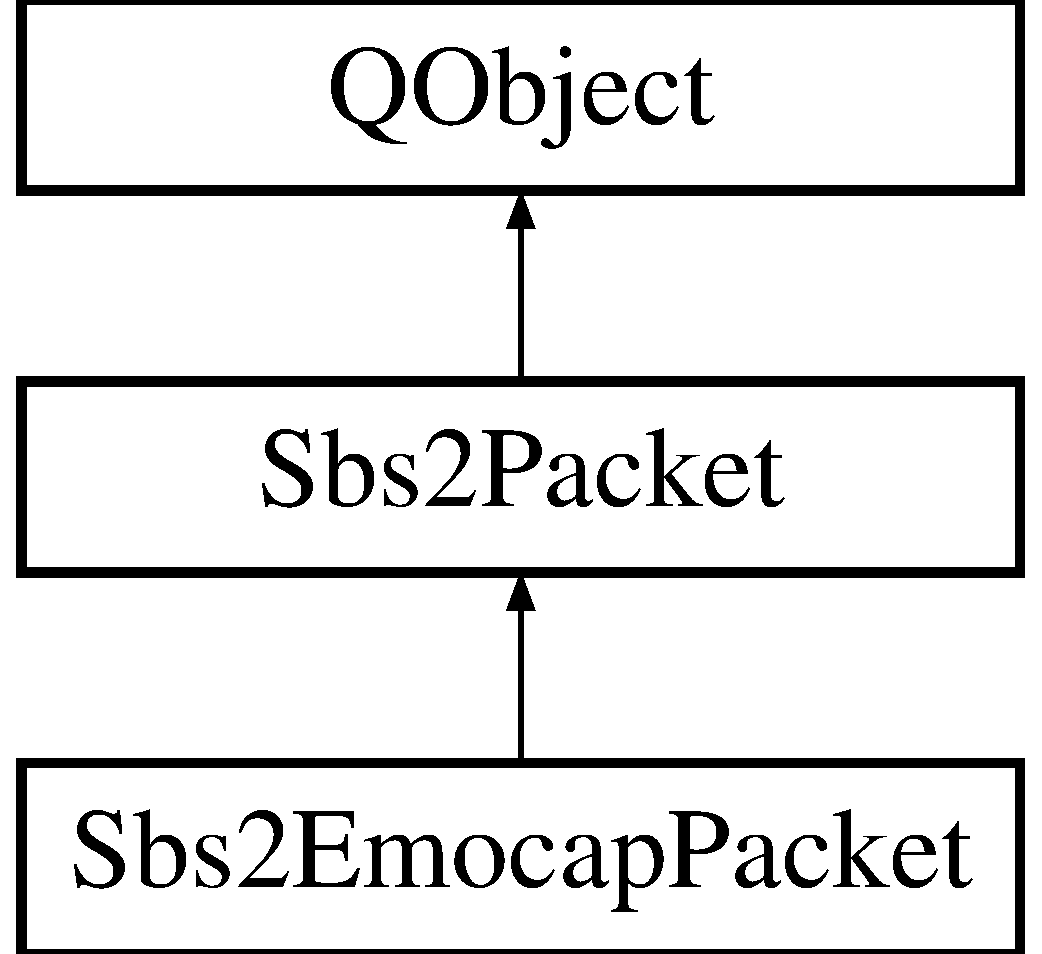
\includegraphics[height=3.000000cm]{classSbs2EmocapPacket}
\end{center}
\end{figure}
\subsection*{Public Member Functions}
\begin{DoxyCompactItemize}
\item 
\hyperlink{classSbs2EmocapPacket_a526fe093d78aec14bd3cb87e108c4f54}{Sbs2\-Emocap\-Packet} (Q\-Object $\ast$parent)
\item 
void \hyperlink{classSbs2EmocapPacket_a68263221ddb233ea7d8da392203a523e}{update} (char $\ast$data)
\begin{DoxyCompactList}\small\item\em Method for updating data in the packet. To avoid continuous creation and destruction of objects, certain number of empty packets is constructed in initialization and then updated with wrap-\/around. Packets should see the raw data delieverd by \hyperlink{classSbs2DataReader}{Sbs2\-Data\-Reader} and form themselves. \end{DoxyCompactList}\end{DoxyCompactItemize}
\subsection*{Additional Inherited Members}


\subsection{Detailed Description}
Smartphone Brain Scanner 2 License Agreement (M\-I\-T License)

Copyright (c) 2012 Arkadiusz Stopczynski, Jakob Eg Larsen, Carsten Stahlhut, Michael Kai Petersen, Lars Kai Hansen. Technical University of Denmark, \hyperlink{namespaceDTU}{D\-T\-U} Informatics, Cognitive Systems Section. \href{http://code.google.com/p/smartphonebrainscanner2}{\tt http\-://code.\-google.\-com/p/smartphonebrainscanner2}

Permission is hereby granted, free of charge, to any person obtaining a copy of this software and associated documentation files (the \char`\"{}\-Software\char`\"{}), to deal in the Software without restriction, including without limitation the rights to use, copy, modify, merge, publish, distribute, sublicense, and/or sell copies of the Software, and to permit persons to whom the Software is furnished to do so, subject to the following conditions\-:

The above copyright notice and this permission notice shall be included in all copies or substantial portions of the Software.

T\-H\-E S\-O\-F\-T\-W\-A\-R\-E I\-S P\-R\-O\-V\-I\-D\-E\-D \char`\"{}\-A\-S I\-S\char`\"{}, W\-I\-T\-H\-O\-U\-T W\-A\-R\-R\-A\-N\-T\-Y O\-F A\-N\-Y K\-I\-N\-D, E\-X\-P\-R\-E\-S\-S O\-R I\-M\-P\-L\-I\-E\-D, I\-N\-C\-L\-U\-D\-I\-N\-G B\-U\-T N\-O\-T L\-I\-M\-I\-T\-E\-D T\-O T\-H\-E W\-A\-R\-R\-A\-N\-T\-I\-E\-S O\-F M\-E\-R\-C\-H\-A\-N\-T\-A\-B\-I\-L\-I\-T\-Y, F\-I\-T\-N\-E\-S\-S F\-O\-R A P\-A\-R\-T\-I\-C\-U\-L\-A\-R P\-U\-R\-P\-O\-S\-E A\-N\-D N\-O\-N\-I\-N\-F\-R\-I\-N\-G\-E\-M\-E\-N\-T. I\-N N\-O E\-V\-E\-N\-T S\-H\-A\-L\-L T\-H\-E A\-U\-T\-H\-O\-R\-S O\-R C\-O\-P\-Y\-R\-I\-G\-H\-T H\-O\-L\-D\-E\-R\-S B\-E L\-I\-A\-B\-L\-E F\-O\-R A\-N\-Y C\-L\-A\-I\-M, D\-A\-M\-A\-G\-E\-S O\-R O\-T\-H\-E\-R L\-I\-A\-B\-I\-L\-I\-T\-Y, W\-H\-E\-T\-H\-E\-R I\-N A\-N A\-C\-T\-I\-O\-N O\-F C\-O\-N\-T\-R\-A\-C\-T, T\-O\-R\-T O\-R O\-T\-H\-E\-R\-W\-I\-S\-E, A\-R\-I\-S\-I\-N\-G F\-R\-O\-M, O\-U\-T O\-F O\-R I\-N C\-O\-N\-N\-E\-C\-T\-I\-O\-N W\-I\-T\-H T\-H\-E S\-O\-F\-T\-W\-A\-R\-E O\-R T\-H\-E U\-S\-E O\-R O\-T\-H\-E\-R D\-E\-A\-L\-I\-N\-G\-S I\-N T\-H\-E S\-O\-F\-T\-W\-A\-R\-E. 

\subsection{Constructor \& Destructor Documentation}
\hypertarget{classSbs2EmocapPacket_a526fe093d78aec14bd3cb87e108c4f54}{\index{Sbs2\-Emocap\-Packet@{Sbs2\-Emocap\-Packet}!Sbs2\-Emocap\-Packet@{Sbs2\-Emocap\-Packet}}
\index{Sbs2\-Emocap\-Packet@{Sbs2\-Emocap\-Packet}!Sbs2EmocapPacket@{Sbs2\-Emocap\-Packet}}
\subsubsection[{Sbs2\-Emocap\-Packet}]{\setlength{\rightskip}{0pt plus 5cm}Sbs2\-Emocap\-Packet\-::\-Sbs2\-Emocap\-Packet (
\begin{DoxyParamCaption}
\item[{Q\-Object $\ast$}]{parent}
\end{DoxyParamCaption}
)}}\label{classSbs2EmocapPacket_a526fe093d78aec14bd3cb87e108c4f54}


\subsection{Member Function Documentation}
\hypertarget{classSbs2EmocapPacket_a68263221ddb233ea7d8da392203a523e}{\index{Sbs2\-Emocap\-Packet@{Sbs2\-Emocap\-Packet}!update@{update}}
\index{update@{update}!Sbs2EmocapPacket@{Sbs2\-Emocap\-Packet}}
\subsubsection[{update}]{\setlength{\rightskip}{0pt plus 5cm}void Sbs2\-Emocap\-Packet\-::update (
\begin{DoxyParamCaption}
\item[{char $\ast$}]{data}
\end{DoxyParamCaption}
)\hspace{0.3cm}{\ttfamily [virtual]}}}\label{classSbs2EmocapPacket_a68263221ddb233ea7d8da392203a523e}


Method for updating data in the packet. To avoid continuous creation and destruction of objects, certain number of empty packets is constructed in initialization and then updated with wrap-\/around. Packets should see the raw data delieverd by \hyperlink{classSbs2DataReader}{Sbs2\-Data\-Reader} and form themselves. 


\begin{DoxyParams}{Parameters}
{\em data} & Pointer to raw data. \\
\hline
\end{DoxyParams}


Reimplemented from \hyperlink{classSbs2Packet_a8b80c76000ceead51e9278c833bb56ae}{Sbs2\-Packet}.



The documentation for this class was generated from the following files\-:\begin{DoxyCompactItemize}
\item 
/media/philipjhj/\-Data/\-One\-Drive/\-Studie/\-Studenterprogrammør/\-S\-B\-S3/smartphonebrainscanner2-\/core/src/hardware/emocap/\hyperlink{sbs2emocappacket_8h}{sbs2emocappacket.\-h}\item 
/media/philipjhj/\-Data/\-One\-Drive/\-Studie/\-Studenterprogrammør/\-S\-B\-S3/smartphonebrainscanner2-\/core/src/hardware/emocap/\hyperlink{sbs2emocappacket_8cpp}{sbs2emocappacket.\-cpp}\end{DoxyCompactItemize}

\hypertarget{classSbs2EmotivDataReader}{\section{Sbs2\-Emotiv\-Data\-Reader Class Reference}
\label{classSbs2EmotivDataReader}\index{Sbs2\-Emotiv\-Data\-Reader@{Sbs2\-Emotiv\-Data\-Reader}}
}


{\ttfamily \#include $<$sbs2emotivdatareader.\-h$>$}

Inheritance diagram for Sbs2\-Emotiv\-Data\-Reader\-:\begin{figure}[H]
\begin{center}
\leavevmode
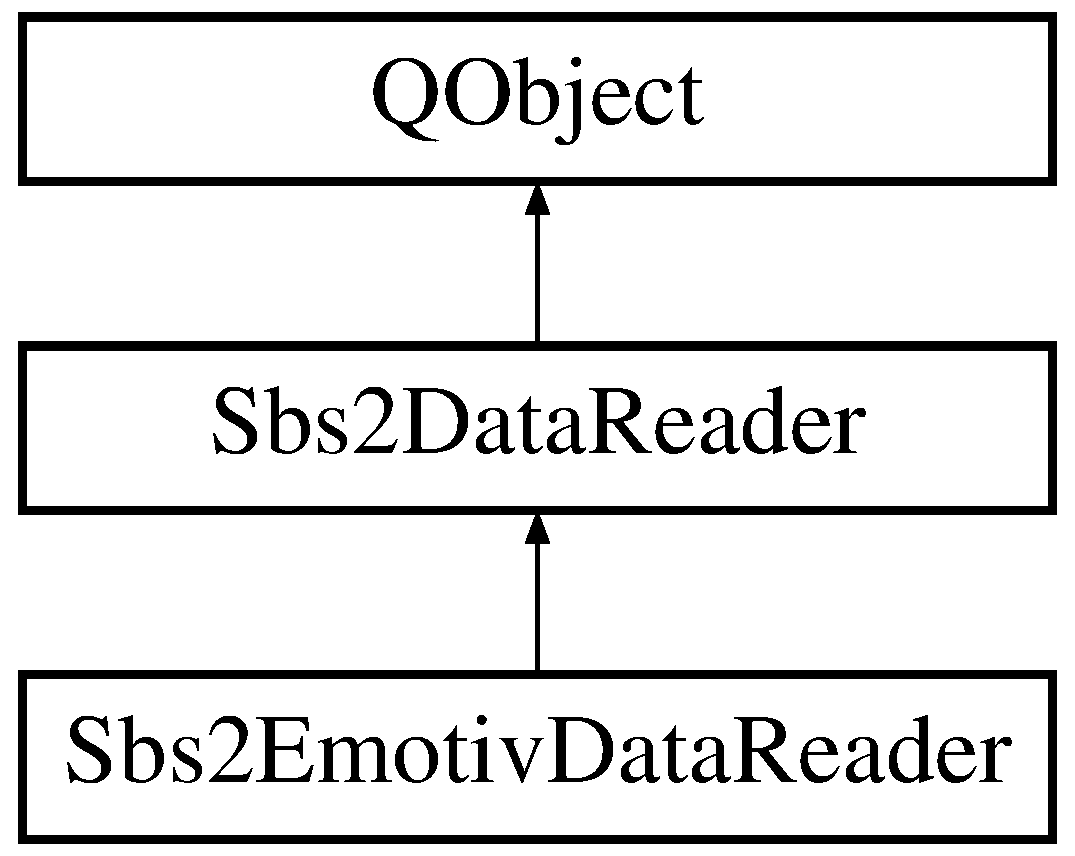
\includegraphics[height=3.000000cm]{classSbs2EmotivDataReader}
\end{center}
\end{figure}
\subsection*{Public Slots}
\begin{DoxyCompactItemize}
\item 
void \hyperlink{classSbs2EmotivDataReader_af767aaebc3232c7690b139ec761e50d0}{device\-Found} (Q\-Map$<$ Q\-String, Q\-Variant $>$ params)
\item 
void \hyperlink{classSbs2EmotivDataReader_a59ce6dc2a270822ab978aaa0c59f1454}{device\-Lost} ()
\item 
void \hyperlink{classSbs2EmotivDataReader_a79159d8649d7d48624f008f5b4c7aa82}{about\-To\-Quit} ()
\item 
void \hyperlink{classSbs2EmotivDataReader_a9eeab9daa04dd01b414519107c286317}{udp\-Data\-Received} (Q\-Vector$<$ char $\ast$ $>$ $\ast$data, int counter)
\item 
void \hyperlink{classSbs2EmotivDataReader_a8da54f965e0c02555009bce9a136b664}{udp\-Data\-Received} (Q\-Udp\-Socket $\ast$raw\-Data\-Udp\-Input\-Socket)
\item 
void \hyperlink{classSbs2EmotivDataReader_a0872b3b86b715697086986b0b0a04dbe}{turn\-Receive\-Udp\-Data\-On} (Q\-String address, int port)
\item 
void \hyperlink{classSbs2EmotivDataReader_aeec17fa711c1497331dc5362468d5e63}{turn\-Receive\-Udp\-Data\-Off} ()
\end{DoxyCompactItemize}
\subsection*{Public Member Functions}
\begin{DoxyCompactItemize}
\item 
\hyperlink{classSbs2EmotivDataReader_af2d1b49542ec2cd354c846e7483aa531}{$\sim$\-Sbs2\-Emotiv\-Data\-Reader} ()
\end{DoxyCompactItemize}
\subsection*{Static Public Member Functions}
\begin{DoxyCompactItemize}
\item 
static \hyperlink{classSbs2EmotivDataReader}{Sbs2\-Emotiv\-Data\-Reader} $\ast$ \hyperlink{classSbs2EmotivDataReader_a5b2be10b38b907f41716830f706991c8}{New} (\hyperlink{classSbs2Callback}{Sbs2\-Callback} $\ast$sbs2\-Callback\-\_\-, int read\-Only\-From\-Network\-\_\-=0, Q\-Object $\ast$parent=0)
\end{DoxyCompactItemize}
\subsection*{Additional Inherited Members}


\subsection{Detailed Description}
Smartphone Brain Scanner 2 License Agreement (M\-I\-T License)

Copyright (c) 2012 Arkadiusz Stopczynski, Jakob Eg Larsen, Carsten Stahlhut, Michael Kai Petersen, Lars Kai Hansen. Technical University of Denmark, \hyperlink{namespaceDTU}{D\-T\-U} Informatics, Cognitive Systems Section. \href{http://code.google.com/p/smartphonebrainscanner2}{\tt http\-://code.\-google.\-com/p/smartphonebrainscanner2}

Permission is hereby granted, free of charge, to any person obtaining a copy of this software and associated documentation files (the \char`\"{}\-Software\char`\"{}), to deal in the Software without restriction, including without limitation the rights to use, copy, modify, merge, publish, distribute, sublicense, and/or sell copies of the Software, and to permit persons to whom the Software is furnished to do so, subject to the following conditions\-:

The above copyright notice and this permission notice shall be included in all copies or substantial portions of the Software.

T\-H\-E S\-O\-F\-T\-W\-A\-R\-E I\-S P\-R\-O\-V\-I\-D\-E\-D \char`\"{}\-A\-S I\-S\char`\"{}, W\-I\-T\-H\-O\-U\-T W\-A\-R\-R\-A\-N\-T\-Y O\-F A\-N\-Y K\-I\-N\-D, E\-X\-P\-R\-E\-S\-S O\-R I\-M\-P\-L\-I\-E\-D, I\-N\-C\-L\-U\-D\-I\-N\-G B\-U\-T N\-O\-T L\-I\-M\-I\-T\-E\-D T\-O T\-H\-E W\-A\-R\-R\-A\-N\-T\-I\-E\-S O\-F M\-E\-R\-C\-H\-A\-N\-T\-A\-B\-I\-L\-I\-T\-Y, F\-I\-T\-N\-E\-S\-S F\-O\-R A P\-A\-R\-T\-I\-C\-U\-L\-A\-R P\-U\-R\-P\-O\-S\-E A\-N\-D N\-O\-N\-I\-N\-F\-R\-I\-N\-G\-E\-M\-E\-N\-T. I\-N N\-O E\-V\-E\-N\-T S\-H\-A\-L\-L T\-H\-E A\-U\-T\-H\-O\-R\-S O\-R C\-O\-P\-Y\-R\-I\-G\-H\-T H\-O\-L\-D\-E\-R\-S B\-E L\-I\-A\-B\-L\-E F\-O\-R A\-N\-Y C\-L\-A\-I\-M, D\-A\-M\-A\-G\-E\-S O\-R O\-T\-H\-E\-R L\-I\-A\-B\-I\-L\-I\-T\-Y, W\-H\-E\-T\-H\-E\-R I\-N A\-N A\-C\-T\-I\-O\-N O\-F C\-O\-N\-T\-R\-A\-C\-T, T\-O\-R\-T O\-R O\-T\-H\-E\-R\-W\-I\-S\-E, A\-R\-I\-S\-I\-N\-G F\-R\-O\-M, O\-U\-T O\-F O\-R I\-N C\-O\-N\-N\-E\-C\-T\-I\-O\-N W\-I\-T\-H T\-H\-E S\-O\-F\-T\-W\-A\-R\-E O\-R T\-H\-E U\-S\-E O\-R O\-T\-H\-E\-R D\-E\-A\-L\-I\-N\-G\-S I\-N T\-H\-E S\-O\-F\-T\-W\-A\-R\-E. 

\subsection{Constructor \& Destructor Documentation}
\hypertarget{classSbs2EmotivDataReader_af2d1b49542ec2cd354c846e7483aa531}{\index{Sbs2\-Emotiv\-Data\-Reader@{Sbs2\-Emotiv\-Data\-Reader}!$\sim$\-Sbs2\-Emotiv\-Data\-Reader@{$\sim$\-Sbs2\-Emotiv\-Data\-Reader}}
\index{$\sim$\-Sbs2\-Emotiv\-Data\-Reader@{$\sim$\-Sbs2\-Emotiv\-Data\-Reader}!Sbs2EmotivDataReader@{Sbs2\-Emotiv\-Data\-Reader}}
\subsubsection[{$\sim$\-Sbs2\-Emotiv\-Data\-Reader}]{\setlength{\rightskip}{0pt plus 5cm}Sbs2\-Emotiv\-Data\-Reader\-::$\sim$\-Sbs2\-Emotiv\-Data\-Reader (
\begin{DoxyParamCaption}
{}
\end{DoxyParamCaption}
)}}\label{classSbs2EmotivDataReader_af2d1b49542ec2cd354c846e7483aa531}


\subsection{Member Function Documentation}
\hypertarget{classSbs2EmotivDataReader_a79159d8649d7d48624f008f5b4c7aa82}{\index{Sbs2\-Emotiv\-Data\-Reader@{Sbs2\-Emotiv\-Data\-Reader}!about\-To\-Quit@{about\-To\-Quit}}
\index{about\-To\-Quit@{about\-To\-Quit}!Sbs2EmotivDataReader@{Sbs2\-Emotiv\-Data\-Reader}}
\subsubsection[{about\-To\-Quit}]{\setlength{\rightskip}{0pt plus 5cm}void Sbs2\-Emotiv\-Data\-Reader\-::about\-To\-Quit (
\begin{DoxyParamCaption}
{}
\end{DoxyParamCaption}
)\hspace{0.3cm}{\ttfamily [slot]}}}\label{classSbs2EmotivDataReader_a79159d8649d7d48624f008f5b4c7aa82}
\hypertarget{classSbs2EmotivDataReader_af767aaebc3232c7690b139ec761e50d0}{\index{Sbs2\-Emotiv\-Data\-Reader@{Sbs2\-Emotiv\-Data\-Reader}!device\-Found@{device\-Found}}
\index{device\-Found@{device\-Found}!Sbs2EmotivDataReader@{Sbs2\-Emotiv\-Data\-Reader}}
\subsubsection[{device\-Found}]{\setlength{\rightskip}{0pt plus 5cm}void Sbs2\-Emotiv\-Data\-Reader\-::device\-Found (
\begin{DoxyParamCaption}
\item[{Q\-Map$<$ Q\-String, Q\-Variant $>$}]{params}
\end{DoxyParamCaption}
)\hspace{0.3cm}{\ttfamily [slot]}}}\label{classSbs2EmotivDataReader_af767aaebc3232c7690b139ec761e50d0}
\hypertarget{classSbs2EmotivDataReader_a59ce6dc2a270822ab978aaa0c59f1454}{\index{Sbs2\-Emotiv\-Data\-Reader@{Sbs2\-Emotiv\-Data\-Reader}!device\-Lost@{device\-Lost}}
\index{device\-Lost@{device\-Lost}!Sbs2EmotivDataReader@{Sbs2\-Emotiv\-Data\-Reader}}
\subsubsection[{device\-Lost}]{\setlength{\rightskip}{0pt plus 5cm}void Sbs2\-Emotiv\-Data\-Reader\-::device\-Lost (
\begin{DoxyParamCaption}
{}
\end{DoxyParamCaption}
)\hspace{0.3cm}{\ttfamily [slot]}}}\label{classSbs2EmotivDataReader_a59ce6dc2a270822ab978aaa0c59f1454}
\hypertarget{classSbs2EmotivDataReader_a5b2be10b38b907f41716830f706991c8}{\index{Sbs2\-Emotiv\-Data\-Reader@{Sbs2\-Emotiv\-Data\-Reader}!New@{New}}
\index{New@{New}!Sbs2EmotivDataReader@{Sbs2\-Emotiv\-Data\-Reader}}
\subsubsection[{New}]{\setlength{\rightskip}{0pt plus 5cm}{\bf Sbs2\-Emotiv\-Data\-Reader} $\ast$ Sbs2\-Emotiv\-Data\-Reader\-::\-New (
\begin{DoxyParamCaption}
\item[{{\bf Sbs2\-Callback} $\ast$}]{sbs2\-Callback\-\_\-, }
\item[{int}]{read\-Only\-From\-Network\-\_\- = {\ttfamily 0}, }
\item[{Q\-Object $\ast$}]{parent = {\ttfamily 0}}
\end{DoxyParamCaption}
)\hspace{0.3cm}{\ttfamily [static]}}}\label{classSbs2EmotivDataReader_a5b2be10b38b907f41716830f706991c8}
\hypertarget{classSbs2EmotivDataReader_aeec17fa711c1497331dc5362468d5e63}{\index{Sbs2\-Emotiv\-Data\-Reader@{Sbs2\-Emotiv\-Data\-Reader}!turn\-Receive\-Udp\-Data\-Off@{turn\-Receive\-Udp\-Data\-Off}}
\index{turn\-Receive\-Udp\-Data\-Off@{turn\-Receive\-Udp\-Data\-Off}!Sbs2EmotivDataReader@{Sbs2\-Emotiv\-Data\-Reader}}
\subsubsection[{turn\-Receive\-Udp\-Data\-Off}]{\setlength{\rightskip}{0pt plus 5cm}void Sbs2\-Emotiv\-Data\-Reader\-::turn\-Receive\-Udp\-Data\-Off (
\begin{DoxyParamCaption}
{}
\end{DoxyParamCaption}
)\hspace{0.3cm}{\ttfamily [slot]}}}\label{classSbs2EmotivDataReader_aeec17fa711c1497331dc5362468d5e63}
\hypertarget{classSbs2EmotivDataReader_a0872b3b86b715697086986b0b0a04dbe}{\index{Sbs2\-Emotiv\-Data\-Reader@{Sbs2\-Emotiv\-Data\-Reader}!turn\-Receive\-Udp\-Data\-On@{turn\-Receive\-Udp\-Data\-On}}
\index{turn\-Receive\-Udp\-Data\-On@{turn\-Receive\-Udp\-Data\-On}!Sbs2EmotivDataReader@{Sbs2\-Emotiv\-Data\-Reader}}
\subsubsection[{turn\-Receive\-Udp\-Data\-On}]{\setlength{\rightskip}{0pt plus 5cm}void Sbs2\-Emotiv\-Data\-Reader\-::turn\-Receive\-Udp\-Data\-On (
\begin{DoxyParamCaption}
\item[{Q\-String}]{address, }
\item[{int}]{port}
\end{DoxyParamCaption}
)\hspace{0.3cm}{\ttfamily [slot]}}}\label{classSbs2EmotivDataReader_a0872b3b86b715697086986b0b0a04dbe}
\hypertarget{classSbs2EmotivDataReader_a9eeab9daa04dd01b414519107c286317}{\index{Sbs2\-Emotiv\-Data\-Reader@{Sbs2\-Emotiv\-Data\-Reader}!udp\-Data\-Received@{udp\-Data\-Received}}
\index{udp\-Data\-Received@{udp\-Data\-Received}!Sbs2EmotivDataReader@{Sbs2\-Emotiv\-Data\-Reader}}
\subsubsection[{udp\-Data\-Received}]{\setlength{\rightskip}{0pt plus 5cm}void Sbs2\-Emotiv\-Data\-Reader\-::udp\-Data\-Received (
\begin{DoxyParamCaption}
\item[{Q\-Vector$<$ char $\ast$ $>$ $\ast$}]{data, }
\item[{int}]{counter}
\end{DoxyParamCaption}
)\hspace{0.3cm}{\ttfamily [slot]}}}\label{classSbs2EmotivDataReader_a9eeab9daa04dd01b414519107c286317}
\hypertarget{classSbs2EmotivDataReader_a8da54f965e0c02555009bce9a136b664}{\index{Sbs2\-Emotiv\-Data\-Reader@{Sbs2\-Emotiv\-Data\-Reader}!udp\-Data\-Received@{udp\-Data\-Received}}
\index{udp\-Data\-Received@{udp\-Data\-Received}!Sbs2EmotivDataReader@{Sbs2\-Emotiv\-Data\-Reader}}
\subsubsection[{udp\-Data\-Received}]{\setlength{\rightskip}{0pt plus 5cm}void Sbs2\-Emotiv\-Data\-Reader\-::udp\-Data\-Received (
\begin{DoxyParamCaption}
\item[{Q\-Udp\-Socket $\ast$}]{raw\-Data\-Udp\-Input\-Socket}
\end{DoxyParamCaption}
)\hspace{0.3cm}{\ttfamily [slot]}}}\label{classSbs2EmotivDataReader_a8da54f965e0c02555009bce9a136b664}


The documentation for this class was generated from the following files\-:\begin{DoxyCompactItemize}
\item 
/media/philipjhj/\-Data/\-One\-Drive/\-Studie/\-Studenterprogrammør/\-S\-B\-S3/smartphonebrainscanner2-\/core/src/hardware/emotiv/\hyperlink{sbs2emotivdatareader_8h}{sbs2emotivdatareader.\-h}\item 
/media/philipjhj/\-Data/\-One\-Drive/\-Studie/\-Studenterprogrammør/\-S\-B\-S3/smartphonebrainscanner2-\/core/src/hardware/emotiv/\hyperlink{sbs2emotivdatareader_8cpp}{sbs2emotivdatareader.\-cpp}\end{DoxyCompactItemize}

\hypertarget{classSbs2EmotivDecryptor}{\section{Sbs2\-Emotiv\-Decryptor Class Reference}
\label{classSbs2EmotivDecryptor}\index{Sbs2\-Emotiv\-Decryptor@{Sbs2\-Emotiv\-Decryptor}}
}


{\ttfamily \#include $<$sbs2emotivdecryptor.\-h$>$}

Inheritance diagram for Sbs2\-Emotiv\-Decryptor\-:\begin{figure}[H]
\begin{center}
\leavevmode
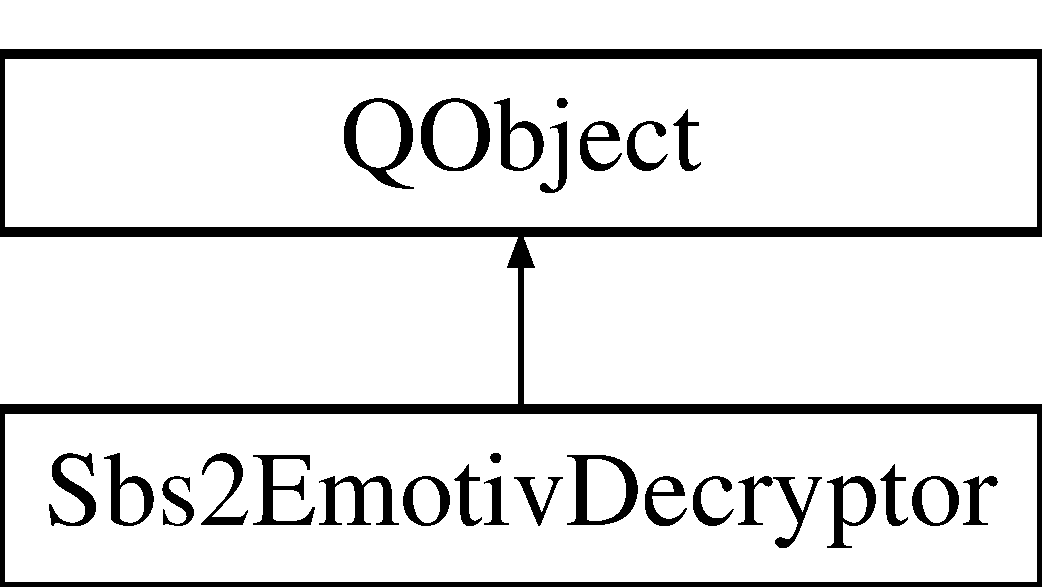
\includegraphics[height=2.000000cm]{classSbs2EmotivDecryptor}
\end{center}
\end{figure}
\subsection*{Public Member Functions}
\begin{DoxyCompactItemize}
\item 
\hyperlink{classSbs2EmotivDecryptor_a2c6aa5b39e471d5eeec155d4a0b0c1e5}{Sbs2\-Emotiv\-Decryptor} (Q\-Object $\ast$parent=0)
\item 
void \hyperlink{classSbs2EmotivDecryptor_a589f85bd37e15e6359b03cfb5d33dceb}{set\-Serial\-Number} (char $\ast$serial\-Number\-\_\-)
\item 
void \hyperlink{classSbs2EmotivDecryptor_af6846ef65ed5168abf367dfa6ef266da}{set\-Serial\-Number} (Q\-String serial\-Number\-\_\-)
\item 
void \hyperlink{classSbs2EmotivDecryptor_ad6dbde08a191bee980f0ebac1658738d}{decrypt} (char cipher\mbox{[}$\,$\mbox{]}, char plain\mbox{[}$\,$\mbox{]})
\end{DoxyCompactItemize}


\subsection{Detailed Description}
Smartphone Brain Scanner 2 License Agreement (M\-I\-T License)

Copyright (c) 2012 Arkadiusz Stopczynski, Jakob Eg Larsen, Carsten Stahlhut, Michael Kai Petersen, Lars Kai Hansen. Technical University of Denmark, \hyperlink{namespaceDTU}{D\-T\-U} Informatics, Cognitive Systems Section. \href{http://code.google.com/p/smartphonebrainscanner2}{\tt http\-://code.\-google.\-com/p/smartphonebrainscanner2}

Permission is hereby granted, free of charge, to any person obtaining a copy of this software and associated documentation files (the \char`\"{}\-Software\char`\"{}), to deal in the Software without restriction, including without limitation the rights to use, copy, modify, merge, publish, distribute, sublicense, and/or sell copies of the Software, and to permit persons to whom the Software is furnished to do so, subject to the following conditions\-:

The above copyright notice and this permission notice shall be included in all copies or substantial portions of the Software.

T\-H\-E S\-O\-F\-T\-W\-A\-R\-E I\-S P\-R\-O\-V\-I\-D\-E\-D \char`\"{}\-A\-S I\-S\char`\"{}, W\-I\-T\-H\-O\-U\-T W\-A\-R\-R\-A\-N\-T\-Y O\-F A\-N\-Y K\-I\-N\-D, E\-X\-P\-R\-E\-S\-S O\-R I\-M\-P\-L\-I\-E\-D, I\-N\-C\-L\-U\-D\-I\-N\-G B\-U\-T N\-O\-T L\-I\-M\-I\-T\-E\-D T\-O T\-H\-E W\-A\-R\-R\-A\-N\-T\-I\-E\-S O\-F M\-E\-R\-C\-H\-A\-N\-T\-A\-B\-I\-L\-I\-T\-Y, F\-I\-T\-N\-E\-S\-S F\-O\-R A P\-A\-R\-T\-I\-C\-U\-L\-A\-R P\-U\-R\-P\-O\-S\-E A\-N\-D N\-O\-N\-I\-N\-F\-R\-I\-N\-G\-E\-M\-E\-N\-T. I\-N N\-O E\-V\-E\-N\-T S\-H\-A\-L\-L T\-H\-E A\-U\-T\-H\-O\-R\-S O\-R C\-O\-P\-Y\-R\-I\-G\-H\-T H\-O\-L\-D\-E\-R\-S B\-E L\-I\-A\-B\-L\-E F\-O\-R A\-N\-Y C\-L\-A\-I\-M, D\-A\-M\-A\-G\-E\-S O\-R O\-T\-H\-E\-R L\-I\-A\-B\-I\-L\-I\-T\-Y, W\-H\-E\-T\-H\-E\-R I\-N A\-N A\-C\-T\-I\-O\-N O\-F C\-O\-N\-T\-R\-A\-C\-T, T\-O\-R\-T O\-R O\-T\-H\-E\-R\-W\-I\-S\-E, A\-R\-I\-S\-I\-N\-G F\-R\-O\-M, O\-U\-T O\-F O\-R I\-N C\-O\-N\-N\-E\-C\-T\-I\-O\-N W\-I\-T\-H T\-H\-E S\-O\-F\-T\-W\-A\-R\-E O\-R T\-H\-E U\-S\-E O\-R O\-T\-H\-E\-R D\-E\-A\-L\-I\-N\-G\-S I\-N T\-H\-E S\-O\-F\-T\-W\-A\-R\-E. 

\subsection{Constructor \& Destructor Documentation}
\hypertarget{classSbs2EmotivDecryptor_a2c6aa5b39e471d5eeec155d4a0b0c1e5}{\index{Sbs2\-Emotiv\-Decryptor@{Sbs2\-Emotiv\-Decryptor}!Sbs2\-Emotiv\-Decryptor@{Sbs2\-Emotiv\-Decryptor}}
\index{Sbs2\-Emotiv\-Decryptor@{Sbs2\-Emotiv\-Decryptor}!Sbs2EmotivDecryptor@{Sbs2\-Emotiv\-Decryptor}}
\subsubsection[{Sbs2\-Emotiv\-Decryptor}]{\setlength{\rightskip}{0pt plus 5cm}Sbs2\-Emotiv\-Decryptor\-::\-Sbs2\-Emotiv\-Decryptor (
\begin{DoxyParamCaption}
\item[{Q\-Object $\ast$}]{parent = {\ttfamily 0}}
\end{DoxyParamCaption}
)\hspace{0.3cm}{\ttfamily [explicit]}}}\label{classSbs2EmotivDecryptor_a2c6aa5b39e471d5eeec155d4a0b0c1e5}


\subsection{Member Function Documentation}
\hypertarget{classSbs2EmotivDecryptor_ad6dbde08a191bee980f0ebac1658738d}{\index{Sbs2\-Emotiv\-Decryptor@{Sbs2\-Emotiv\-Decryptor}!decrypt@{decrypt}}
\index{decrypt@{decrypt}!Sbs2EmotivDecryptor@{Sbs2\-Emotiv\-Decryptor}}
\subsubsection[{decrypt}]{\setlength{\rightskip}{0pt plus 5cm}void Sbs2\-Emotiv\-Decryptor\-::decrypt (
\begin{DoxyParamCaption}
\item[{char}]{cipher\mbox{[}$\,$\mbox{]}, }
\item[{char}]{plain\mbox{[}$\,$\mbox{]}}
\end{DoxyParamCaption}
)}}\label{classSbs2EmotivDecryptor_ad6dbde08a191bee980f0ebac1658738d}
\hypertarget{classSbs2EmotivDecryptor_a589f85bd37e15e6359b03cfb5d33dceb}{\index{Sbs2\-Emotiv\-Decryptor@{Sbs2\-Emotiv\-Decryptor}!set\-Serial\-Number@{set\-Serial\-Number}}
\index{set\-Serial\-Number@{set\-Serial\-Number}!Sbs2EmotivDecryptor@{Sbs2\-Emotiv\-Decryptor}}
\subsubsection[{set\-Serial\-Number}]{\setlength{\rightskip}{0pt plus 5cm}void Sbs2\-Emotiv\-Decryptor\-::set\-Serial\-Number (
\begin{DoxyParamCaption}
\item[{char $\ast$}]{serial\-Number\-\_\-}
\end{DoxyParamCaption}
)}}\label{classSbs2EmotivDecryptor_a589f85bd37e15e6359b03cfb5d33dceb}
\hypertarget{classSbs2EmotivDecryptor_af6846ef65ed5168abf367dfa6ef266da}{\index{Sbs2\-Emotiv\-Decryptor@{Sbs2\-Emotiv\-Decryptor}!set\-Serial\-Number@{set\-Serial\-Number}}
\index{set\-Serial\-Number@{set\-Serial\-Number}!Sbs2EmotivDecryptor@{Sbs2\-Emotiv\-Decryptor}}
\subsubsection[{set\-Serial\-Number}]{\setlength{\rightskip}{0pt plus 5cm}void Sbs2\-Emotiv\-Decryptor\-::set\-Serial\-Number (
\begin{DoxyParamCaption}
\item[{Q\-String}]{serial\-Number\-\_\-}
\end{DoxyParamCaption}
)}}\label{classSbs2EmotivDecryptor_af6846ef65ed5168abf367dfa6ef266da}


The documentation for this class was generated from the following files\-:\begin{DoxyCompactItemize}
\item 
/media/philipjhj/\-Data/\-One\-Drive/\-Studie/\-Studenterprogrammør/\-S\-B\-S3/smartphonebrainscanner2-\/core/src/hardware/emotiv/\hyperlink{sbs2emotivdecryptor_8h}{sbs2emotivdecryptor.\-h}\item 
/media/philipjhj/\-Data/\-One\-Drive/\-Studie/\-Studenterprogrammør/\-S\-B\-S3/smartphonebrainscanner2-\/core/src/hardware/emotiv/\hyperlink{sbs2emotivdecryptor__dummy_8cpp}{sbs2emotivdecryptor\-\_\-dummy.\-cpp}\end{DoxyCompactItemize}

\hypertarget{classSbs2EmotivMounter}{\section{Sbs2\-Emotiv\-Mounter Class Reference}
\label{classSbs2EmotivMounter}\index{Sbs2\-Emotiv\-Mounter@{Sbs2\-Emotiv\-Mounter}}
}


{\ttfamily \#include $<$sbs2emotivmounter.\-h$>$}

Inheritance diagram for Sbs2\-Emotiv\-Mounter\-:\begin{figure}[H]
\begin{center}
\leavevmode
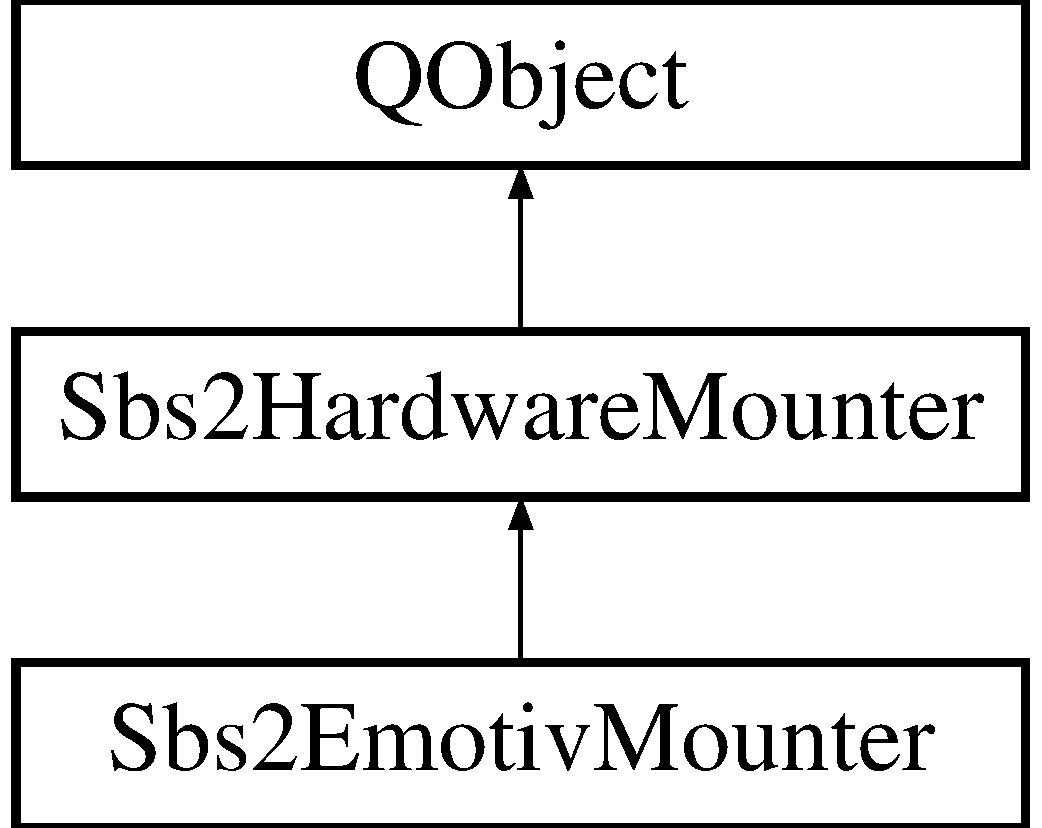
\includegraphics[height=3.000000cm]{classSbs2EmotivMounter}
\end{center}
\end{figure}
\subsection*{Public Slots}
\begin{DoxyCompactItemize}
\item 
void \hyperlink{classSbs2EmotivMounter_a2888e172fdb5428ae4c620be9b6686c4}{start} ()
\item 
void \hyperlink{classSbs2EmotivMounter_a4e0000fb5e7f3eed5dd6e9c9e7b35217}{stop} ()
\item 
void \hyperlink{classSbs2EmotivMounter_af730039b8d644ca1af6661b2ba7bb240}{invalidate} ()
\end{DoxyCompactItemize}
\subsection*{Public Member Functions}
\begin{DoxyCompactItemize}
\item 
\hyperlink{classSbs2EmotivMounter_a1a1e666cc3e7fb3229400fa98ebc831e}{$\sim$\-Sbs2\-Emotiv\-Mounter} ()
\end{DoxyCompactItemize}
\subsection*{Static Public Member Functions}
\begin{DoxyCompactItemize}
\item 
static \hyperlink{classSbs2EmotivMounter}{Sbs2\-Emotiv\-Mounter} $\ast$ \hyperlink{classSbs2EmotivMounter_a9326cef45222dc1fdb5064e4460f9ceb}{New} (Q\-Object $\ast$parent=0)
\end{DoxyCompactItemize}
\subsection*{Additional Inherited Members}


\subsection{Detailed Description}
Smartphone Brain Scanner 2 License Agreement (M\-I\-T License)

Copyright (c) 2012 Arkadiusz Stopczynski, Jakob Eg Larsen, Carsten Stahlhut, Michael Kai Petersen, Lars Kai Hansen. Technical University of Denmark, \hyperlink{namespaceDTU}{D\-T\-U} Informatics, Cognitive Systems Section. \href{http://code.google.com/p/smartphonebrainscanner2}{\tt http\-://code.\-google.\-com/p/smartphonebrainscanner2}

Permission is hereby granted, free of charge, to any person obtaining a copy of this software and associated documentation files (the \char`\"{}\-Software\char`\"{}), to deal in the Software without restriction, including without limitation the rights to use, copy, modify, merge, publish, distribute, sublicense, and/or sell copies of the Software, and to permit persons to whom the Software is furnished to do so, subject to the following conditions\-:

The above copyright notice and this permission notice shall be included in all copies or substantial portions of the Software.

T\-H\-E S\-O\-F\-T\-W\-A\-R\-E I\-S P\-R\-O\-V\-I\-D\-E\-D \char`\"{}\-A\-S I\-S\char`\"{}, W\-I\-T\-H\-O\-U\-T W\-A\-R\-R\-A\-N\-T\-Y O\-F A\-N\-Y K\-I\-N\-D, E\-X\-P\-R\-E\-S\-S O\-R I\-M\-P\-L\-I\-E\-D, I\-N\-C\-L\-U\-D\-I\-N\-G B\-U\-T N\-O\-T L\-I\-M\-I\-T\-E\-D T\-O T\-H\-E W\-A\-R\-R\-A\-N\-T\-I\-E\-S O\-F M\-E\-R\-C\-H\-A\-N\-T\-A\-B\-I\-L\-I\-T\-Y, F\-I\-T\-N\-E\-S\-S F\-O\-R A P\-A\-R\-T\-I\-C\-U\-L\-A\-R P\-U\-R\-P\-O\-S\-E A\-N\-D N\-O\-N\-I\-N\-F\-R\-I\-N\-G\-E\-M\-E\-N\-T. I\-N N\-O E\-V\-E\-N\-T S\-H\-A\-L\-L T\-H\-E A\-U\-T\-H\-O\-R\-S O\-R C\-O\-P\-Y\-R\-I\-G\-H\-T H\-O\-L\-D\-E\-R\-S B\-E L\-I\-A\-B\-L\-E F\-O\-R A\-N\-Y C\-L\-A\-I\-M, D\-A\-M\-A\-G\-E\-S O\-R O\-T\-H\-E\-R L\-I\-A\-B\-I\-L\-I\-T\-Y, W\-H\-E\-T\-H\-E\-R I\-N A\-N A\-C\-T\-I\-O\-N O\-F C\-O\-N\-T\-R\-A\-C\-T, T\-O\-R\-T O\-R O\-T\-H\-E\-R\-W\-I\-S\-E, A\-R\-I\-S\-I\-N\-G F\-R\-O\-M, O\-U\-T O\-F O\-R I\-N C\-O\-N\-N\-E\-C\-T\-I\-O\-N W\-I\-T\-H T\-H\-E S\-O\-F\-T\-W\-A\-R\-E O\-R T\-H\-E U\-S\-E O\-R O\-T\-H\-E\-R D\-E\-A\-L\-I\-N\-G\-S I\-N T\-H\-E S\-O\-F\-T\-W\-A\-R\-E.\-On O\-S\-X we use hidapi to access raw data. 

\subsection{Constructor \& Destructor Documentation}
\hypertarget{classSbs2EmotivMounter_a1a1e666cc3e7fb3229400fa98ebc831e}{\index{Sbs2\-Emotiv\-Mounter@{Sbs2\-Emotiv\-Mounter}!$\sim$\-Sbs2\-Emotiv\-Mounter@{$\sim$\-Sbs2\-Emotiv\-Mounter}}
\index{$\sim$\-Sbs2\-Emotiv\-Mounter@{$\sim$\-Sbs2\-Emotiv\-Mounter}!Sbs2EmotivMounter@{Sbs2\-Emotiv\-Mounter}}
\subsubsection[{$\sim$\-Sbs2\-Emotiv\-Mounter}]{\setlength{\rightskip}{0pt plus 5cm}Sbs2\-Emotiv\-Mounter\-::$\sim$\-Sbs2\-Emotiv\-Mounter (
\begin{DoxyParamCaption}
{}
\end{DoxyParamCaption}
)}}\label{classSbs2EmotivMounter_a1a1e666cc3e7fb3229400fa98ebc831e}


\subsection{Member Function Documentation}
\hypertarget{classSbs2EmotivMounter_af730039b8d644ca1af6661b2ba7bb240}{\index{Sbs2\-Emotiv\-Mounter@{Sbs2\-Emotiv\-Mounter}!invalidate@{invalidate}}
\index{invalidate@{invalidate}!Sbs2EmotivMounter@{Sbs2\-Emotiv\-Mounter}}
\subsubsection[{invalidate}]{\setlength{\rightskip}{0pt plus 5cm}void Sbs2\-Emotiv\-Mounter\-::invalidate (
\begin{DoxyParamCaption}
{}
\end{DoxyParamCaption}
)\hspace{0.3cm}{\ttfamily [slot]}}}\label{classSbs2EmotivMounter_af730039b8d644ca1af6661b2ba7bb240}
\hypertarget{classSbs2EmotivMounter_a9326cef45222dc1fdb5064e4460f9ceb}{\index{Sbs2\-Emotiv\-Mounter@{Sbs2\-Emotiv\-Mounter}!New@{New}}
\index{New@{New}!Sbs2EmotivMounter@{Sbs2\-Emotiv\-Mounter}}
\subsubsection[{New}]{\setlength{\rightskip}{0pt plus 5cm}{\bf Sbs2\-Emotiv\-Mounter} $\ast$ Sbs2\-Emotiv\-Mounter\-::\-New (
\begin{DoxyParamCaption}
\item[{Q\-Object $\ast$}]{parent = {\ttfamily 0}}
\end{DoxyParamCaption}
)\hspace{0.3cm}{\ttfamily [static]}}}\label{classSbs2EmotivMounter_a9326cef45222dc1fdb5064e4460f9ceb}
\hypertarget{classSbs2EmotivMounter_a2888e172fdb5428ae4c620be9b6686c4}{\index{Sbs2\-Emotiv\-Mounter@{Sbs2\-Emotiv\-Mounter}!start@{start}}
\index{start@{start}!Sbs2EmotivMounter@{Sbs2\-Emotiv\-Mounter}}
\subsubsection[{start}]{\setlength{\rightskip}{0pt plus 5cm}void Sbs2\-Emotiv\-Mounter\-::start (
\begin{DoxyParamCaption}
{}
\end{DoxyParamCaption}
)\hspace{0.3cm}{\ttfamily [slot]}}}\label{classSbs2EmotivMounter_a2888e172fdb5428ae4c620be9b6686c4}
\hypertarget{classSbs2EmotivMounter_a4e0000fb5e7f3eed5dd6e9c9e7b35217}{\index{Sbs2\-Emotiv\-Mounter@{Sbs2\-Emotiv\-Mounter}!stop@{stop}}
\index{stop@{stop}!Sbs2EmotivMounter@{Sbs2\-Emotiv\-Mounter}}
\subsubsection[{stop}]{\setlength{\rightskip}{0pt plus 5cm}void Sbs2\-Emotiv\-Mounter\-::stop (
\begin{DoxyParamCaption}
{}
\end{DoxyParamCaption}
)\hspace{0.3cm}{\ttfamily [slot]}}}\label{classSbs2EmotivMounter_a4e0000fb5e7f3eed5dd6e9c9e7b35217}


The documentation for this class was generated from the following files\-:\begin{DoxyCompactItemize}
\item 
/media/philipjhj/\-Data/\-One\-Drive/\-Studie/\-Studenterprogrammør/\-S\-B\-S3/smartphonebrainscanner2-\/core/src/hardware/emotiv/\hyperlink{sbs2emotivmounter_8h}{sbs2emotivmounter.\-h}\item 
/media/philipjhj/\-Data/\-One\-Drive/\-Studie/\-Studenterprogrammør/\-S\-B\-S3/smartphonebrainscanner2-\/core/src/hardware/emotiv/\hyperlink{sbs2emotivmounter_8cpp}{sbs2emotivmounter.\-cpp}\end{DoxyCompactItemize}

\hypertarget{classSbs2EmotivPacket}{\section{Sbs2\-Emotiv\-Packet Class Reference}
\label{classSbs2EmotivPacket}\index{Sbs2\-Emotiv\-Packet@{Sbs2\-Emotiv\-Packet}}
}


{\ttfamily \#include $<$sbs2emotivpacket.\-h$>$}

Inheritance diagram for Sbs2\-Emotiv\-Packet\-:\begin{figure}[H]
\begin{center}
\leavevmode
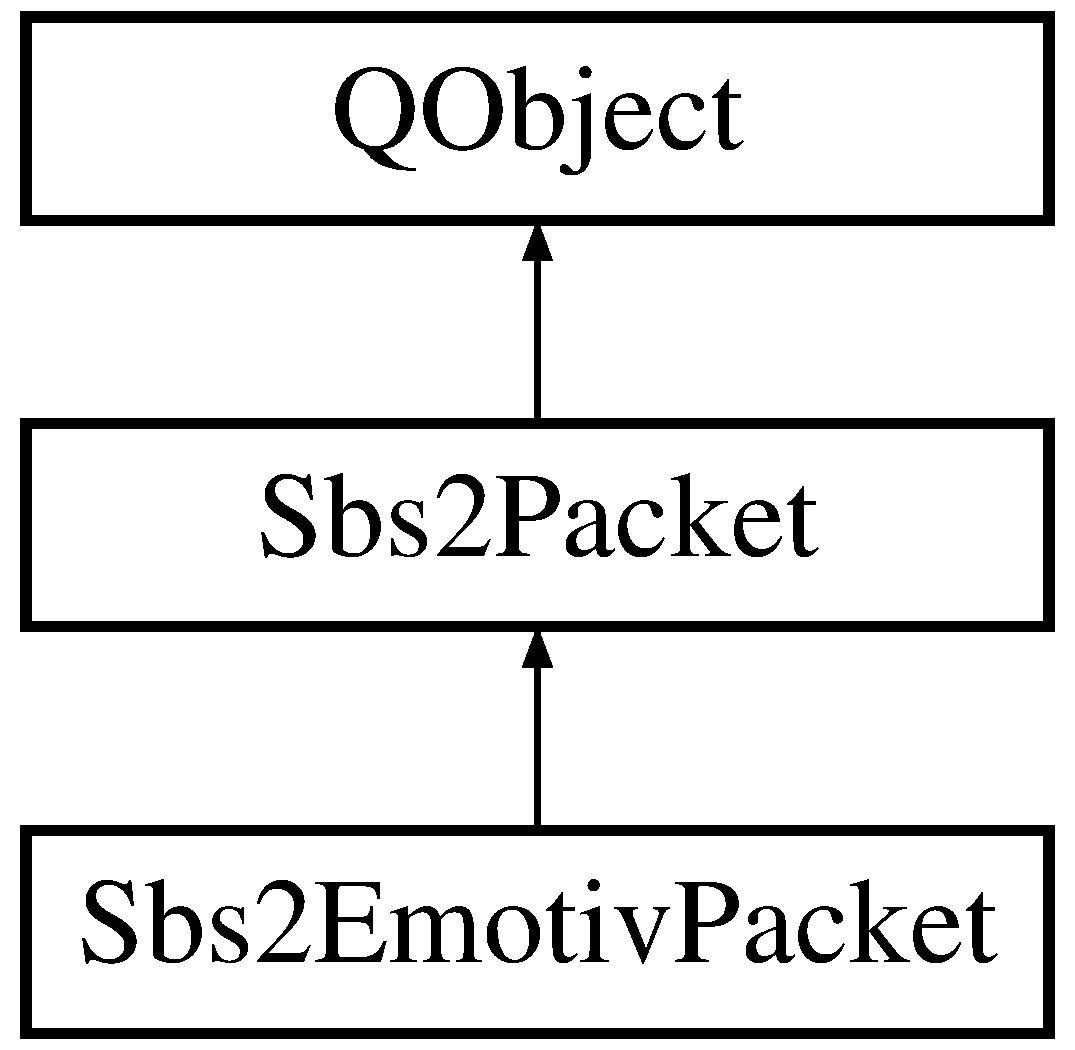
\includegraphics[height=3.000000cm]{classSbs2EmotivPacket}
\end{center}
\end{figure}
\subsection*{Public Member Functions}
\begin{DoxyCompactItemize}
\item 
\hyperlink{classSbs2EmotivPacket_a05de077593ed85a082584fb212221388}{Sbs2\-Emotiv\-Packet} (Q\-Object $\ast$parent)
\item 
void \hyperlink{classSbs2EmotivPacket_aaf8b25e8f747bbb80d7dcc5853d6e814}{update} (char $\ast$data)
\begin{DoxyCompactList}\small\item\em Method for updating data in the packet. To avoid continuous creation and destruction of objects, certain number of empty packets is constructed in initialization and then updated with wrap-\/around. Packets should see the raw data delieverd by \hyperlink{classSbs2DataReader}{Sbs2\-Data\-Reader} and form themselves. \end{DoxyCompactList}\end{DoxyCompactItemize}
\subsection*{Additional Inherited Members}


\subsection{Detailed Description}
Smartphone Brain Scanner 2 License Agreement (M\-I\-T License)

Copyright (c) 2012 Arkadiusz Stopczynski, Jakob Eg Larsen, Carsten Stahlhut, Michael Kai Petersen, Lars Kai Hansen. Technical University of Denmark, \hyperlink{namespaceDTU}{D\-T\-U} Informatics, Cognitive Systems Section. \href{http://code.google.com/p/smartphonebrainscanner2}{\tt http\-://code.\-google.\-com/p/smartphonebrainscanner2}

Permission is hereby granted, free of charge, to any person obtaining a copy of this software and associated documentation files (the \char`\"{}\-Software\char`\"{}), to deal in the Software without restriction, including without limitation the rights to use, copy, modify, merge, publish, distribute, sublicense, and/or sell copies of the Software, and to permit persons to whom the Software is furnished to do so, subject to the following conditions\-:

The above copyright notice and this permission notice shall be included in all copies or substantial portions of the Software.

T\-H\-E S\-O\-F\-T\-W\-A\-R\-E I\-S P\-R\-O\-V\-I\-D\-E\-D \char`\"{}\-A\-S I\-S\char`\"{}, W\-I\-T\-H\-O\-U\-T W\-A\-R\-R\-A\-N\-T\-Y O\-F A\-N\-Y K\-I\-N\-D, E\-X\-P\-R\-E\-S\-S O\-R I\-M\-P\-L\-I\-E\-D, I\-N\-C\-L\-U\-D\-I\-N\-G B\-U\-T N\-O\-T L\-I\-M\-I\-T\-E\-D T\-O T\-H\-E W\-A\-R\-R\-A\-N\-T\-I\-E\-S O\-F M\-E\-R\-C\-H\-A\-N\-T\-A\-B\-I\-L\-I\-T\-Y, F\-I\-T\-N\-E\-S\-S F\-O\-R A P\-A\-R\-T\-I\-C\-U\-L\-A\-R P\-U\-R\-P\-O\-S\-E A\-N\-D N\-O\-N\-I\-N\-F\-R\-I\-N\-G\-E\-M\-E\-N\-T. I\-N N\-O E\-V\-E\-N\-T S\-H\-A\-L\-L T\-H\-E A\-U\-T\-H\-O\-R\-S O\-R C\-O\-P\-Y\-R\-I\-G\-H\-T H\-O\-L\-D\-E\-R\-S B\-E L\-I\-A\-B\-L\-E F\-O\-R A\-N\-Y C\-L\-A\-I\-M, D\-A\-M\-A\-G\-E\-S O\-R O\-T\-H\-E\-R L\-I\-A\-B\-I\-L\-I\-T\-Y, W\-H\-E\-T\-H\-E\-R I\-N A\-N A\-C\-T\-I\-O\-N O\-F C\-O\-N\-T\-R\-A\-C\-T, T\-O\-R\-T O\-R O\-T\-H\-E\-R\-W\-I\-S\-E, A\-R\-I\-S\-I\-N\-G F\-R\-O\-M, O\-U\-T O\-F O\-R I\-N C\-O\-N\-N\-E\-C\-T\-I\-O\-N W\-I\-T\-H T\-H\-E S\-O\-F\-T\-W\-A\-R\-E O\-R T\-H\-E U\-S\-E O\-R O\-T\-H\-E\-R D\-E\-A\-L\-I\-N\-G\-S I\-N T\-H\-E S\-O\-F\-T\-W\-A\-R\-E. 

\subsection{Constructor \& Destructor Documentation}
\hypertarget{classSbs2EmotivPacket_a05de077593ed85a082584fb212221388}{\index{Sbs2\-Emotiv\-Packet@{Sbs2\-Emotiv\-Packet}!Sbs2\-Emotiv\-Packet@{Sbs2\-Emotiv\-Packet}}
\index{Sbs2\-Emotiv\-Packet@{Sbs2\-Emotiv\-Packet}!Sbs2EmotivPacket@{Sbs2\-Emotiv\-Packet}}
\subsubsection[{Sbs2\-Emotiv\-Packet}]{\setlength{\rightskip}{0pt plus 5cm}Sbs2\-Emotiv\-Packet\-::\-Sbs2\-Emotiv\-Packet (
\begin{DoxyParamCaption}
\item[{Q\-Object $\ast$}]{parent}
\end{DoxyParamCaption}
)}}\label{classSbs2EmotivPacket_a05de077593ed85a082584fb212221388}


\subsection{Member Function Documentation}
\hypertarget{classSbs2EmotivPacket_aaf8b25e8f747bbb80d7dcc5853d6e814}{\index{Sbs2\-Emotiv\-Packet@{Sbs2\-Emotiv\-Packet}!update@{update}}
\index{update@{update}!Sbs2EmotivPacket@{Sbs2\-Emotiv\-Packet}}
\subsubsection[{update}]{\setlength{\rightskip}{0pt plus 5cm}void Sbs2\-Emotiv\-Packet\-::update (
\begin{DoxyParamCaption}
\item[{char $\ast$}]{data}
\end{DoxyParamCaption}
)\hspace{0.3cm}{\ttfamily [virtual]}}}\label{classSbs2EmotivPacket_aaf8b25e8f747bbb80d7dcc5853d6e814}


Method for updating data in the packet. To avoid continuous creation and destruction of objects, certain number of empty packets is constructed in initialization and then updated with wrap-\/around. Packets should see the raw data delieverd by \hyperlink{classSbs2DataReader}{Sbs2\-Data\-Reader} and form themselves. 


\begin{DoxyParams}{Parameters}
{\em data} & Pointer to raw data. \\
\hline
\end{DoxyParams}


Reimplemented from \hyperlink{classSbs2Packet_a8b80c76000ceead51e9278c833bb56ae}{Sbs2\-Packet}.



The documentation for this class was generated from the following files\-:\begin{DoxyCompactItemize}
\item 
/media/philipjhj/\-Data/\-One\-Drive/\-Studie/\-Studenterprogrammør/\-S\-B\-S3/smartphonebrainscanner2-\/core/src/hardware/emotiv/\hyperlink{sbs2emotivpacket_8h}{sbs2emotivpacket.\-h}\item 
/media/philipjhj/\-Data/\-One\-Drive/\-Studie/\-Studenterprogrammør/\-S\-B\-S3/smartphonebrainscanner2-\/core/src/hardware/emotiv/\hyperlink{sbs2emotivpacket_8cpp}{sbs2emotivpacket.\-cpp}\end{DoxyCompactItemize}

\hypertarget{classSbs2FakeDataReader}{\section{Sbs2\-Fake\-Data\-Reader Class Reference}
\label{classSbs2FakeDataReader}\index{Sbs2\-Fake\-Data\-Reader@{Sbs2\-Fake\-Data\-Reader}}
}


{\ttfamily \#include $<$sbs2fakedatareader.\-h$>$}

Inheritance diagram for Sbs2\-Fake\-Data\-Reader\-:\begin{figure}[H]
\begin{center}
\leavevmode
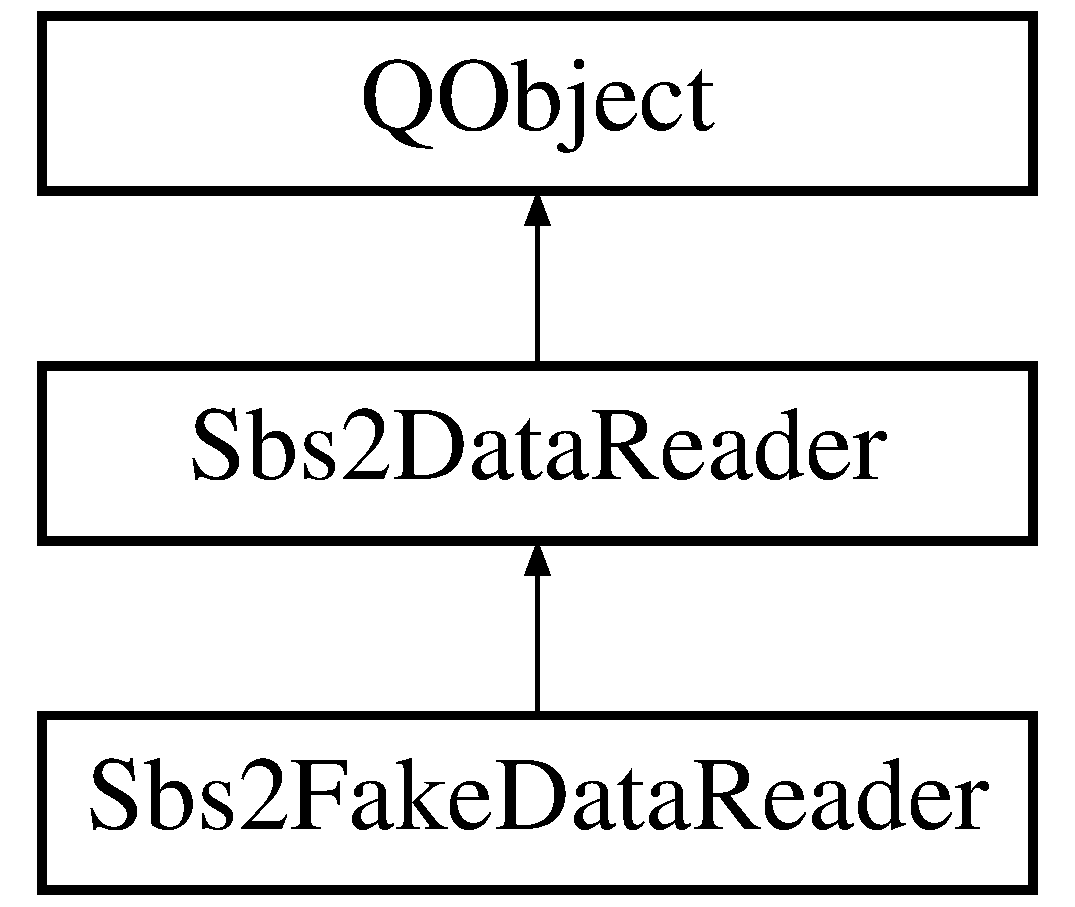
\includegraphics[height=3.000000cm]{classSbs2FakeDataReader}
\end{center}
\end{figure}
\subsection*{Public Slots}
\begin{DoxyCompactItemize}
\item 
void \hyperlink{classSbs2FakeDataReader_a89b47ade19abce4ce863ca827baf3bb8}{start} ()
\item 
void \hyperlink{classSbs2FakeDataReader_a7d83fefb103e473fcd65d93dbd0e89fd}{stop} ()
\item 
void \hyperlink{classSbs2FakeDataReader_ab9ffd9d2c27dd41a5640363841fd03a5}{set\-Filename} (Q\-String filename\-\_\-)
\end{DoxyCompactItemize}
\subsection*{Public Member Functions}
\begin{DoxyCompactItemize}
\item 
\hyperlink{classSbs2FakeDataReader_a275a5b0012846476934a3707af931c78}{$\sim$\-Sbs2\-Fake\-Data\-Reader} ()
\end{DoxyCompactItemize}
\subsection*{Static Public Member Functions}
\begin{DoxyCompactItemize}
\item 
static \hyperlink{classSbs2FakeDataReader}{Sbs2\-Fake\-Data\-Reader} $\ast$ \hyperlink{classSbs2FakeDataReader_a1321841227262ea5fc574439f99b7e75}{New} (\hyperlink{classSbs2Callback}{Sbs2\-Callback} $\ast$sbs2\-Callback\-\_\-, int read\-Only\-From\-Network\-\_\-=0, Q\-Object $\ast$parent=0)
\end{DoxyCompactItemize}
\subsection*{Additional Inherited Members}


\subsection{Constructor \& Destructor Documentation}
\hypertarget{classSbs2FakeDataReader_a275a5b0012846476934a3707af931c78}{\index{Sbs2\-Fake\-Data\-Reader@{Sbs2\-Fake\-Data\-Reader}!$\sim$\-Sbs2\-Fake\-Data\-Reader@{$\sim$\-Sbs2\-Fake\-Data\-Reader}}
\index{$\sim$\-Sbs2\-Fake\-Data\-Reader@{$\sim$\-Sbs2\-Fake\-Data\-Reader}!Sbs2FakeDataReader@{Sbs2\-Fake\-Data\-Reader}}
\subsubsection[{$\sim$\-Sbs2\-Fake\-Data\-Reader}]{\setlength{\rightskip}{0pt plus 5cm}Sbs2\-Fake\-Data\-Reader\-::$\sim$\-Sbs2\-Fake\-Data\-Reader (
\begin{DoxyParamCaption}
{}
\end{DoxyParamCaption}
)}}\label{classSbs2FakeDataReader_a275a5b0012846476934a3707af931c78}


\subsection{Member Function Documentation}
\hypertarget{classSbs2FakeDataReader_a1321841227262ea5fc574439f99b7e75}{\index{Sbs2\-Fake\-Data\-Reader@{Sbs2\-Fake\-Data\-Reader}!New@{New}}
\index{New@{New}!Sbs2FakeDataReader@{Sbs2\-Fake\-Data\-Reader}}
\subsubsection[{New}]{\setlength{\rightskip}{0pt plus 5cm}{\bf Sbs2\-Fake\-Data\-Reader} $\ast$ Sbs2\-Fake\-Data\-Reader\-::\-New (
\begin{DoxyParamCaption}
\item[{{\bf Sbs2\-Callback} $\ast$}]{sbs2\-Callback\-\_\-, }
\item[{int}]{read\-Only\-From\-Network\-\_\- = {\ttfamily 0}, }
\item[{Q\-Object $\ast$}]{parent = {\ttfamily 0}}
\end{DoxyParamCaption}
)\hspace{0.3cm}{\ttfamily [static]}}}\label{classSbs2FakeDataReader_a1321841227262ea5fc574439f99b7e75}
\hypertarget{classSbs2FakeDataReader_ab9ffd9d2c27dd41a5640363841fd03a5}{\index{Sbs2\-Fake\-Data\-Reader@{Sbs2\-Fake\-Data\-Reader}!set\-Filename@{set\-Filename}}
\index{set\-Filename@{set\-Filename}!Sbs2FakeDataReader@{Sbs2\-Fake\-Data\-Reader}}
\subsubsection[{set\-Filename}]{\setlength{\rightskip}{0pt plus 5cm}void Sbs2\-Fake\-Data\-Reader\-::set\-Filename (
\begin{DoxyParamCaption}
\item[{Q\-String}]{filename\-\_\-}
\end{DoxyParamCaption}
)\hspace{0.3cm}{\ttfamily [inline]}, {\ttfamily [slot]}}}\label{classSbs2FakeDataReader_ab9ffd9d2c27dd41a5640363841fd03a5}
\hypertarget{classSbs2FakeDataReader_a89b47ade19abce4ce863ca827baf3bb8}{\index{Sbs2\-Fake\-Data\-Reader@{Sbs2\-Fake\-Data\-Reader}!start@{start}}
\index{start@{start}!Sbs2FakeDataReader@{Sbs2\-Fake\-Data\-Reader}}
\subsubsection[{start}]{\setlength{\rightskip}{0pt plus 5cm}void Sbs2\-Fake\-Data\-Reader\-::start (
\begin{DoxyParamCaption}
{}
\end{DoxyParamCaption}
)\hspace{0.3cm}{\ttfamily [slot]}}}\label{classSbs2FakeDataReader_a89b47ade19abce4ce863ca827baf3bb8}
\hypertarget{classSbs2FakeDataReader_a7d83fefb103e473fcd65d93dbd0e89fd}{\index{Sbs2\-Fake\-Data\-Reader@{Sbs2\-Fake\-Data\-Reader}!stop@{stop}}
\index{stop@{stop}!Sbs2FakeDataReader@{Sbs2\-Fake\-Data\-Reader}}
\subsubsection[{stop}]{\setlength{\rightskip}{0pt plus 5cm}void Sbs2\-Fake\-Data\-Reader\-::stop (
\begin{DoxyParamCaption}
{}
\end{DoxyParamCaption}
)\hspace{0.3cm}{\ttfamily [inline]}, {\ttfamily [slot]}}}\label{classSbs2FakeDataReader_a7d83fefb103e473fcd65d93dbd0e89fd}


The documentation for this class was generated from the following files\-:\begin{DoxyCompactItemize}
\item 
/media/philipjhj/\-Data/\-One\-Drive/\-Studie/\-Studenterprogrammør/\-S\-B\-S3/smartphonebrainscanner2-\/core/src/hardware/fake/\hyperlink{sbs2fakedatareader_8h}{sbs2fakedatareader.\-h}\item 
/media/philipjhj/\-Data/\-One\-Drive/\-Studie/\-Studenterprogrammør/\-S\-B\-S3/smartphonebrainscanner2-\/core/src/hardware/fake/\hyperlink{sbs2fakedatareader_8cpp}{sbs2fakedatareader.\-cpp}\end{DoxyCompactItemize}

\hypertarget{classSbs2FakePacket}{\section{Sbs2\-Fake\-Packet Class Reference}
\label{classSbs2FakePacket}\index{Sbs2\-Fake\-Packet@{Sbs2\-Fake\-Packet}}
}


{\ttfamily \#include $<$sbs2fakepacket.\-h$>$}

Inheritance diagram for Sbs2\-Fake\-Packet\-:\begin{figure}[H]
\begin{center}
\leavevmode
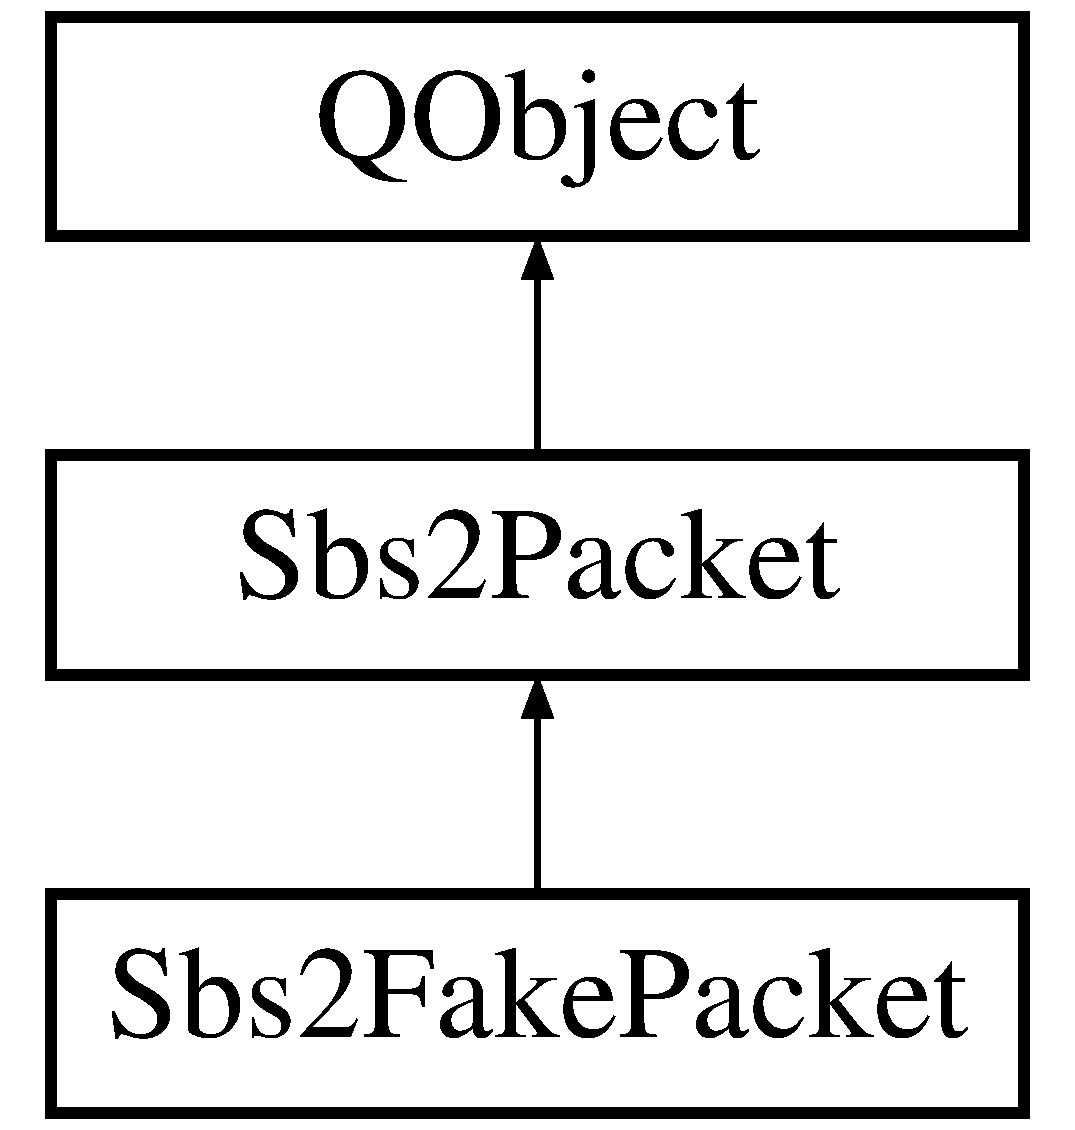
\includegraphics[height=3.000000cm]{classSbs2FakePacket}
\end{center}
\end{figure}
\subsection*{Public Member Functions}
\begin{DoxyCompactItemize}
\item 
\hyperlink{classSbs2FakePacket_a1942a4ef7edb4057a8de46769a4acd77}{Sbs2\-Fake\-Packet} (Q\-Object $\ast$parent)
\item 
void \hyperlink{classSbs2FakePacket_aa11764514e8d26feef1b6c8862b0deb6}{update} (double $\ast$data)
\end{DoxyCompactItemize}
\subsection*{Additional Inherited Members}


\subsection{Constructor \& Destructor Documentation}
\hypertarget{classSbs2FakePacket_a1942a4ef7edb4057a8de46769a4acd77}{\index{Sbs2\-Fake\-Packet@{Sbs2\-Fake\-Packet}!Sbs2\-Fake\-Packet@{Sbs2\-Fake\-Packet}}
\index{Sbs2\-Fake\-Packet@{Sbs2\-Fake\-Packet}!Sbs2FakePacket@{Sbs2\-Fake\-Packet}}
\subsubsection[{Sbs2\-Fake\-Packet}]{\setlength{\rightskip}{0pt plus 5cm}Sbs2\-Fake\-Packet\-::\-Sbs2\-Fake\-Packet (
\begin{DoxyParamCaption}
\item[{Q\-Object $\ast$}]{parent}
\end{DoxyParamCaption}
)}}\label{classSbs2FakePacket_a1942a4ef7edb4057a8de46769a4acd77}


\subsection{Member Function Documentation}
\hypertarget{classSbs2FakePacket_aa11764514e8d26feef1b6c8862b0deb6}{\index{Sbs2\-Fake\-Packet@{Sbs2\-Fake\-Packet}!update@{update}}
\index{update@{update}!Sbs2FakePacket@{Sbs2\-Fake\-Packet}}
\subsubsection[{update}]{\setlength{\rightskip}{0pt plus 5cm}void Sbs2\-Fake\-Packet\-::update (
\begin{DoxyParamCaption}
\item[{double $\ast$}]{data}
\end{DoxyParamCaption}
)}}\label{classSbs2FakePacket_aa11764514e8d26feef1b6c8862b0deb6}


The documentation for this class was generated from the following files\-:\begin{DoxyCompactItemize}
\item 
/media/philipjhj/\-Data/\-One\-Drive/\-Studie/\-Studenterprogrammør/\-S\-B\-S3/smartphonebrainscanner2-\/core/src/hardware/fake/\hyperlink{sbs2fakepacket_8h}{sbs2fakepacket.\-h}\item 
/media/philipjhj/\-Data/\-One\-Drive/\-Studie/\-Studenterprogrammør/\-S\-B\-S3/smartphonebrainscanner2-\/core/src/hardware/fake/\hyperlink{sbs2fakepacket_8cpp}{sbs2fakepacket.\-cpp}\end{DoxyCompactItemize}

\hypertarget{classSbs2FileHandler}{\section{Sbs2\-File\-Handler Class Reference}
\label{classSbs2FileHandler}\index{Sbs2\-File\-Handler@{Sbs2\-File\-Handler}}
}


{\ttfamily \#include $<$sbs2filehandler.\-h$>$}

Inheritance diagram for Sbs2\-File\-Handler\-:\begin{figure}[H]
\begin{center}
\leavevmode
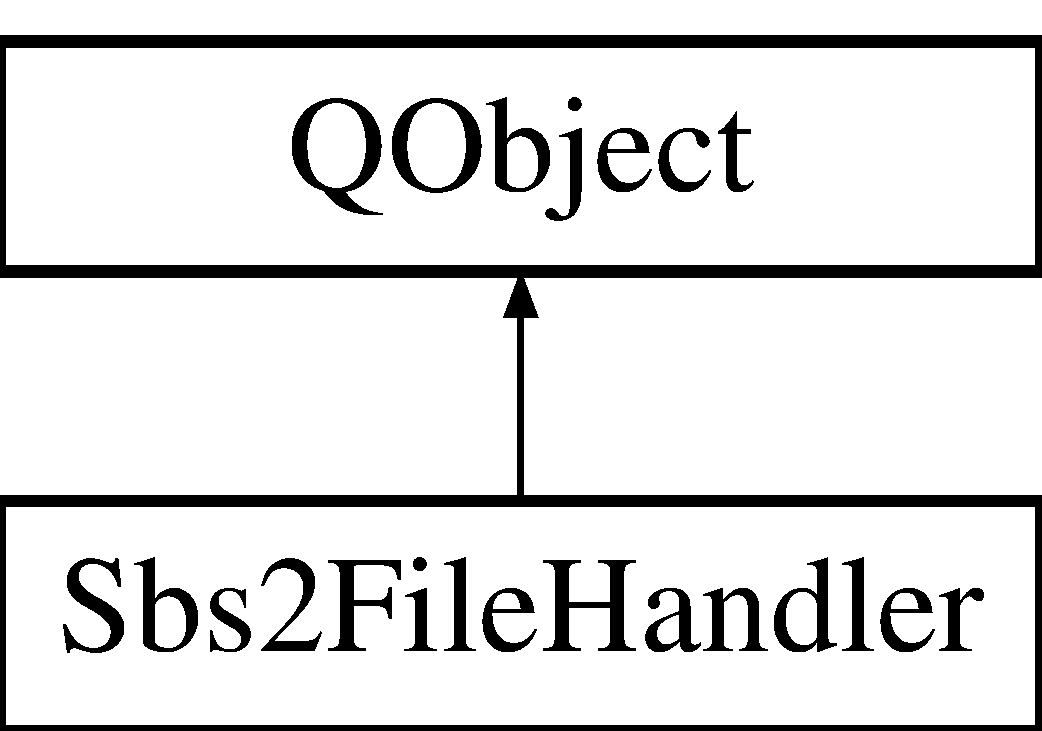
\includegraphics[height=2.000000cm]{classSbs2FileHandler}
\end{center}
\end{figure}
\subsection*{Public Slots}
\begin{DoxyCompactItemize}
\item 
void \hyperlink{classSbs2FileHandler_a2b5bc147768ba76d694045fc8163a07f}{insert\-Into\-Meta\-File} (Q\-String event)
\item 
void \hyperlink{classSbs2FileHandler_a981682a2485188e1aeea82d87d58844e}{close} ()
\item 
void \hyperlink{classSbs2FileHandler_a129918680fb23627ee734402bc6382fa}{create\-Meta\-File} (Q\-String user\-\_\-, Q\-String description\-\_\-)
\end{DoxyCompactItemize}
\subsection*{Public Member Functions}
\begin{DoxyCompactItemize}
\item 
void \hyperlink{classSbs2FileHandler_a4a2767712909e5437bbb9d1a81ba88b2}{dump\-Raw\-Data} (char $\ast$raw\-Data)
\item 
\hyperlink{classSbs2FileHandler_a311041e7ee81403d0371f1d95f223979}{$\sim$\-Sbs2\-File\-Handler} ()
\item 
Q\-String \hyperlink{classSbs2FileHandler_aa1636922d6cf30c6efece6eb8114d14c}{get\-Raw\-Filename} ()
\item 
int \hyperlink{classSbs2FileHandler_adaa22c27c0fdd391478e437e88781b51}{get\-Packet\-Zero} ()
\end{DoxyCompactItemize}
\subsection*{Static Public Member Functions}
\begin{DoxyCompactItemize}
\item 
static \hyperlink{classSbs2FileHandler}{Sbs2\-File\-Handler} $\ast$ \hyperlink{classSbs2FileHandler_a3f219d55c277ff005a90cdf92ce0411b}{New} (Q\-Object $\ast$parent=0)
\end{DoxyCompactItemize}


\subsection{Detailed Description}
Smartphone Brain Scanner 2 License Agreement (M\-I\-T License)

Copyright (c) 2012 Arkadiusz Stopczynski, Jakob Eg Larsen, Carsten Stahlhut, Michael Kai Petersen, Lars Kai Hansen. Technical University of Denmark, \hyperlink{namespaceDTU}{D\-T\-U} Informatics, Cognitive Systems Section. \href{http://code.google.com/p/smartphonebrainscanner2}{\tt http\-://code.\-google.\-com/p/smartphonebrainscanner2}

Permission is hereby granted, free of charge, to any person obtaining a copy of this software and associated documentation files (the \char`\"{}\-Software\char`\"{}), to deal in the Software without restriction, including without limitation the rights to use, copy, modify, merge, publish, distribute, sublicense, and/or sell copies of the Software, and to permit persons to whom the Software is furnished to do so, subject to the following conditions\-:

The above copyright notice and this permission notice shall be included in all copies or substantial portions of the Software.

T\-H\-E S\-O\-F\-T\-W\-A\-R\-E I\-S P\-R\-O\-V\-I\-D\-E\-D \char`\"{}\-A\-S I\-S\char`\"{}, W\-I\-T\-H\-O\-U\-T W\-A\-R\-R\-A\-N\-T\-Y O\-F A\-N\-Y K\-I\-N\-D, E\-X\-P\-R\-E\-S\-S O\-R I\-M\-P\-L\-I\-E\-D, I\-N\-C\-L\-U\-D\-I\-N\-G B\-U\-T N\-O\-T L\-I\-M\-I\-T\-E\-D T\-O T\-H\-E W\-A\-R\-R\-A\-N\-T\-I\-E\-S O\-F M\-E\-R\-C\-H\-A\-N\-T\-A\-B\-I\-L\-I\-T\-Y, F\-I\-T\-N\-E\-S\-S F\-O\-R A P\-A\-R\-T\-I\-C\-U\-L\-A\-R P\-U\-R\-P\-O\-S\-E A\-N\-D N\-O\-N\-I\-N\-F\-R\-I\-N\-G\-E\-M\-E\-N\-T. I\-N N\-O E\-V\-E\-N\-T S\-H\-A\-L\-L T\-H\-E A\-U\-T\-H\-O\-R\-S O\-R C\-O\-P\-Y\-R\-I\-G\-H\-T H\-O\-L\-D\-E\-R\-S B\-E L\-I\-A\-B\-L\-E F\-O\-R A\-N\-Y C\-L\-A\-I\-M, D\-A\-M\-A\-G\-E\-S O\-R O\-T\-H\-E\-R L\-I\-A\-B\-I\-L\-I\-T\-Y, W\-H\-E\-T\-H\-E\-R I\-N A\-N A\-C\-T\-I\-O\-N O\-F C\-O\-N\-T\-R\-A\-C\-T, T\-O\-R\-T O\-R O\-T\-H\-E\-R\-W\-I\-S\-E, A\-R\-I\-S\-I\-N\-G F\-R\-O\-M, O\-U\-T O\-F O\-R I\-N C\-O\-N\-N\-E\-C\-T\-I\-O\-N W\-I\-T\-H T\-H\-E S\-O\-F\-T\-W\-A\-R\-E O\-R T\-H\-E U\-S\-E O\-R O\-T\-H\-E\-R D\-E\-A\-L\-I\-N\-G\-S I\-N T\-H\-E S\-O\-F\-T\-W\-A\-R\-E. 

\subsection{Constructor \& Destructor Documentation}
\hypertarget{classSbs2FileHandler_a311041e7ee81403d0371f1d95f223979}{\index{Sbs2\-File\-Handler@{Sbs2\-File\-Handler}!$\sim$\-Sbs2\-File\-Handler@{$\sim$\-Sbs2\-File\-Handler}}
\index{$\sim$\-Sbs2\-File\-Handler@{$\sim$\-Sbs2\-File\-Handler}!Sbs2FileHandler@{Sbs2\-File\-Handler}}
\subsubsection[{$\sim$\-Sbs2\-File\-Handler}]{\setlength{\rightskip}{0pt plus 5cm}Sbs2\-File\-Handler\-::$\sim$\-Sbs2\-File\-Handler (
\begin{DoxyParamCaption}
{}
\end{DoxyParamCaption}
)}}\label{classSbs2FileHandler_a311041e7ee81403d0371f1d95f223979}


\subsection{Member Function Documentation}
\hypertarget{classSbs2FileHandler_a981682a2485188e1aeea82d87d58844e}{\index{Sbs2\-File\-Handler@{Sbs2\-File\-Handler}!close@{close}}
\index{close@{close}!Sbs2FileHandler@{Sbs2\-File\-Handler}}
\subsubsection[{close}]{\setlength{\rightskip}{0pt plus 5cm}void Sbs2\-File\-Handler\-::close (
\begin{DoxyParamCaption}
{}
\end{DoxyParamCaption}
)\hspace{0.3cm}{\ttfamily [slot]}}}\label{classSbs2FileHandler_a981682a2485188e1aeea82d87d58844e}
\hypertarget{classSbs2FileHandler_a129918680fb23627ee734402bc6382fa}{\index{Sbs2\-File\-Handler@{Sbs2\-File\-Handler}!create\-Meta\-File@{create\-Meta\-File}}
\index{create\-Meta\-File@{create\-Meta\-File}!Sbs2FileHandler@{Sbs2\-File\-Handler}}
\subsubsection[{create\-Meta\-File}]{\setlength{\rightskip}{0pt plus 5cm}void Sbs2\-File\-Handler\-::create\-Meta\-File (
\begin{DoxyParamCaption}
\item[{Q\-String}]{user\-\_\-, }
\item[{Q\-String}]{description\-\_\-}
\end{DoxyParamCaption}
)\hspace{0.3cm}{\ttfamily [slot]}}}\label{classSbs2FileHandler_a129918680fb23627ee734402bc6382fa}
\hypertarget{classSbs2FileHandler_a4a2767712909e5437bbb9d1a81ba88b2}{\index{Sbs2\-File\-Handler@{Sbs2\-File\-Handler}!dump\-Raw\-Data@{dump\-Raw\-Data}}
\index{dump\-Raw\-Data@{dump\-Raw\-Data}!Sbs2FileHandler@{Sbs2\-File\-Handler}}
\subsubsection[{dump\-Raw\-Data}]{\setlength{\rightskip}{0pt plus 5cm}void Sbs2\-File\-Handler\-::dump\-Raw\-Data (
\begin{DoxyParamCaption}
\item[{char $\ast$}]{raw\-Data}
\end{DoxyParamCaption}
)}}\label{classSbs2FileHandler_a4a2767712909e5437bbb9d1a81ba88b2}
\hypertarget{classSbs2FileHandler_adaa22c27c0fdd391478e437e88781b51}{\index{Sbs2\-File\-Handler@{Sbs2\-File\-Handler}!get\-Packet\-Zero@{get\-Packet\-Zero}}
\index{get\-Packet\-Zero@{get\-Packet\-Zero}!Sbs2FileHandler@{Sbs2\-File\-Handler}}
\subsubsection[{get\-Packet\-Zero}]{\setlength{\rightskip}{0pt plus 5cm}int Sbs2\-File\-Handler\-::get\-Packet\-Zero (
\begin{DoxyParamCaption}
{}
\end{DoxyParamCaption}
)}}\label{classSbs2FileHandler_adaa22c27c0fdd391478e437e88781b51}
\hypertarget{classSbs2FileHandler_aa1636922d6cf30c6efece6eb8114d14c}{\index{Sbs2\-File\-Handler@{Sbs2\-File\-Handler}!get\-Raw\-Filename@{get\-Raw\-Filename}}
\index{get\-Raw\-Filename@{get\-Raw\-Filename}!Sbs2FileHandler@{Sbs2\-File\-Handler}}
\subsubsection[{get\-Raw\-Filename}]{\setlength{\rightskip}{0pt plus 5cm}Q\-String Sbs2\-File\-Handler\-::get\-Raw\-Filename (
\begin{DoxyParamCaption}
{}
\end{DoxyParamCaption}
)}}\label{classSbs2FileHandler_aa1636922d6cf30c6efece6eb8114d14c}
\hypertarget{classSbs2FileHandler_a2b5bc147768ba76d694045fc8163a07f}{\index{Sbs2\-File\-Handler@{Sbs2\-File\-Handler}!insert\-Into\-Meta\-File@{insert\-Into\-Meta\-File}}
\index{insert\-Into\-Meta\-File@{insert\-Into\-Meta\-File}!Sbs2FileHandler@{Sbs2\-File\-Handler}}
\subsubsection[{insert\-Into\-Meta\-File}]{\setlength{\rightskip}{0pt plus 5cm}void Sbs2\-File\-Handler\-::insert\-Into\-Meta\-File (
\begin{DoxyParamCaption}
\item[{Q\-String}]{event}
\end{DoxyParamCaption}
)\hspace{0.3cm}{\ttfamily [slot]}}}\label{classSbs2FileHandler_a2b5bc147768ba76d694045fc8163a07f}
\hypertarget{classSbs2FileHandler_a3f219d55c277ff005a90cdf92ce0411b}{\index{Sbs2\-File\-Handler@{Sbs2\-File\-Handler}!New@{New}}
\index{New@{New}!Sbs2FileHandler@{Sbs2\-File\-Handler}}
\subsubsection[{New}]{\setlength{\rightskip}{0pt plus 5cm}{\bf Sbs2\-File\-Handler} $\ast$ Sbs2\-File\-Handler\-::\-New (
\begin{DoxyParamCaption}
\item[{Q\-Object $\ast$}]{parent = {\ttfamily 0}}
\end{DoxyParamCaption}
)\hspace{0.3cm}{\ttfamily [static]}}}\label{classSbs2FileHandler_a3f219d55c277ff005a90cdf92ce0411b}


The documentation for this class was generated from the following files\-:\begin{DoxyCompactItemize}
\item 
/media/philipjhj/\-Data/\-One\-Drive/\-Studie/\-Studenterprogrammør/\-S\-B\-S3/smartphonebrainscanner2-\/core/src/\hyperlink{sbs2filehandler_8h}{sbs2filehandler.\-h}\item 
/media/philipjhj/\-Data/\-One\-Drive/\-Studie/\-Studenterprogrammør/\-S\-B\-S3/smartphonebrainscanner2-\/core/src/\hyperlink{sbs2filehandler_8cpp}{sbs2filehandler.\-cpp}\end{DoxyCompactItemize}

\hypertarget{classSbs2Filter}{\section{Sbs2\-Filter Class Reference}
\label{classSbs2Filter}\index{Sbs2\-Filter@{Sbs2\-Filter}}
}


{\ttfamily \#include $<$sbs2filter.\-h$>$}

Inheritance diagram for Sbs2\-Filter\-:\begin{figure}[H]
\begin{center}
\leavevmode
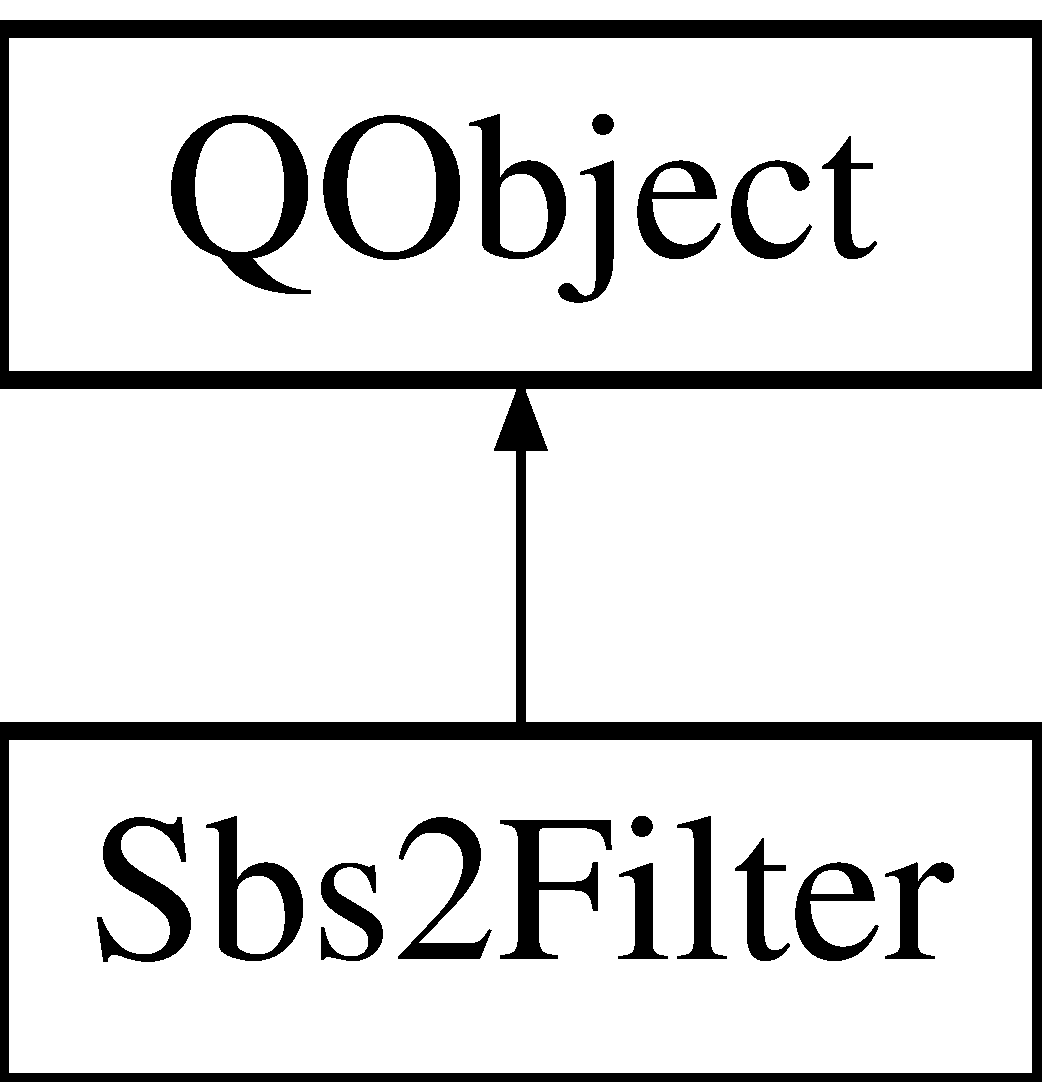
\includegraphics[height=2.000000cm]{classSbs2Filter}
\end{center}
\end{figure}
\subsection*{Public Member Functions}
\begin{DoxyCompactItemize}
\item 
void \hyperlink{classSbs2Filter_a8558f399923de358f6d5f26b66316a9f}{load\-Filter} ()
\item 
void \hyperlink{classSbs2Filter_ad0b72e2a6993a3bddf04f4ad109f1f24}{update\-Filter} (int order\-\_\-, int fband\-Low\-\_\-, int fband\-High\-\_\-)
\item 
void \hyperlink{classSbs2Filter_aebd19b521ed3947f2b95880f84d15b32}{do\-Filter} (\hyperlink{classDTU_1_1DtuArray2D}{D\-T\-U\-::\-Dtu\-Array2\-D}$<$ double $>$ $\ast$values, \hyperlink{classDTU_1_1DtuArray2D}{D\-T\-U\-::\-Dtu\-Array2\-D}$<$ double $>$ $\ast$return\-Values)
\item 
\hyperlink{classSbs2Filter_a48d41a9be977d691a54dff195ef01f94}{$\sim$\-Sbs2\-Filter} ()
\end{DoxyCompactItemize}
\subsection*{Static Public Member Functions}
\begin{DoxyCompactItemize}
\item 
static \hyperlink{classSbs2Filter}{Sbs2\-Filter} $\ast$ \hyperlink{classSbs2Filter_a33d3f76111ff92d1fbbd12cb971e9926}{New} (int fband\-Low\-\_\-, int fband\-High\-\_\-, int order\-\_\-, Q\-Object $\ast$parent=0)
\end{DoxyCompactItemize}


\subsection{Constructor \& Destructor Documentation}
\hypertarget{classSbs2Filter_a48d41a9be977d691a54dff195ef01f94}{\index{Sbs2\-Filter@{Sbs2\-Filter}!$\sim$\-Sbs2\-Filter@{$\sim$\-Sbs2\-Filter}}
\index{$\sim$\-Sbs2\-Filter@{$\sim$\-Sbs2\-Filter}!Sbs2Filter@{Sbs2\-Filter}}
\subsubsection[{$\sim$\-Sbs2\-Filter}]{\setlength{\rightskip}{0pt plus 5cm}Sbs2\-Filter\-::$\sim$\-Sbs2\-Filter (
\begin{DoxyParamCaption}
{}
\end{DoxyParamCaption}
)}}\label{classSbs2Filter_a48d41a9be977d691a54dff195ef01f94}


\subsection{Member Function Documentation}
\hypertarget{classSbs2Filter_aebd19b521ed3947f2b95880f84d15b32}{\index{Sbs2\-Filter@{Sbs2\-Filter}!do\-Filter@{do\-Filter}}
\index{do\-Filter@{do\-Filter}!Sbs2Filter@{Sbs2\-Filter}}
\subsubsection[{do\-Filter}]{\setlength{\rightskip}{0pt plus 5cm}void Sbs2\-Filter\-::do\-Filter (
\begin{DoxyParamCaption}
\item[{{\bf D\-T\-U\-::\-Dtu\-Array2\-D}$<$ double $>$ $\ast$}]{values, }
\item[{{\bf D\-T\-U\-::\-Dtu\-Array2\-D}$<$ double $>$ $\ast$}]{return\-Values}
\end{DoxyParamCaption}
)}}\label{classSbs2Filter_aebd19b521ed3947f2b95880f84d15b32}
\hypertarget{classSbs2Filter_a8558f399923de358f6d5f26b66316a9f}{\index{Sbs2\-Filter@{Sbs2\-Filter}!load\-Filter@{load\-Filter}}
\index{load\-Filter@{load\-Filter}!Sbs2Filter@{Sbs2\-Filter}}
\subsubsection[{load\-Filter}]{\setlength{\rightskip}{0pt plus 5cm}void Sbs2\-Filter\-::load\-Filter (
\begin{DoxyParamCaption}
{}
\end{DoxyParamCaption}
)}}\label{classSbs2Filter_a8558f399923de358f6d5f26b66316a9f}
\hypertarget{classSbs2Filter_a33d3f76111ff92d1fbbd12cb971e9926}{\index{Sbs2\-Filter@{Sbs2\-Filter}!New@{New}}
\index{New@{New}!Sbs2Filter@{Sbs2\-Filter}}
\subsubsection[{New}]{\setlength{\rightskip}{0pt plus 5cm}{\bf Sbs2\-Filter} $\ast$ Sbs2\-Filter\-::\-New (
\begin{DoxyParamCaption}
\item[{int}]{fband\-Low\-\_\-, }
\item[{int}]{fband\-High\-\_\-, }
\item[{int}]{order\-\_\-, }
\item[{Q\-Object $\ast$}]{parent = {\ttfamily 0}}
\end{DoxyParamCaption}
)\hspace{0.3cm}{\ttfamily [static]}}}\label{classSbs2Filter_a33d3f76111ff92d1fbbd12cb971e9926}
\hypertarget{classSbs2Filter_ad0b72e2a6993a3bddf04f4ad109f1f24}{\index{Sbs2\-Filter@{Sbs2\-Filter}!update\-Filter@{update\-Filter}}
\index{update\-Filter@{update\-Filter}!Sbs2Filter@{Sbs2\-Filter}}
\subsubsection[{update\-Filter}]{\setlength{\rightskip}{0pt plus 5cm}void Sbs2\-Filter\-::update\-Filter (
\begin{DoxyParamCaption}
\item[{int}]{order\-\_\-, }
\item[{int}]{fband\-Low\-\_\-, }
\item[{int}]{fband\-High\-\_\-}
\end{DoxyParamCaption}
)}}\label{classSbs2Filter_ad0b72e2a6993a3bddf04f4ad109f1f24}


The documentation for this class was generated from the following files\-:\begin{DoxyCompactItemize}
\item 
/media/philipjhj/\-Data/\-One\-Drive/\-Studie/\-Studenterprogrammør/\-S\-B\-S3/smartphonebrainscanner2-\/core/src/\hyperlink{sbs2filter_8h}{sbs2filter.\-h}\item 
/media/philipjhj/\-Data/\-One\-Drive/\-Studie/\-Studenterprogrammør/\-S\-B\-S3/smartphonebrainscanner2-\/core/src/\hyperlink{sbs2filter_8cpp}{sbs2filter.\-cpp}\end{DoxyCompactItemize}

\hypertarget{classSbs2HardwareMounter}{\section{Sbs2\-Hardware\-Mounter Class Reference}
\label{classSbs2HardwareMounter}\index{Sbs2\-Hardware\-Mounter@{Sbs2\-Hardware\-Mounter}}
}


{\ttfamily \#include $<$sbs2hardwaremounter.\-h$>$}

Inheritance diagram for Sbs2\-Hardware\-Mounter\-:\begin{figure}[H]
\begin{center}
\leavevmode
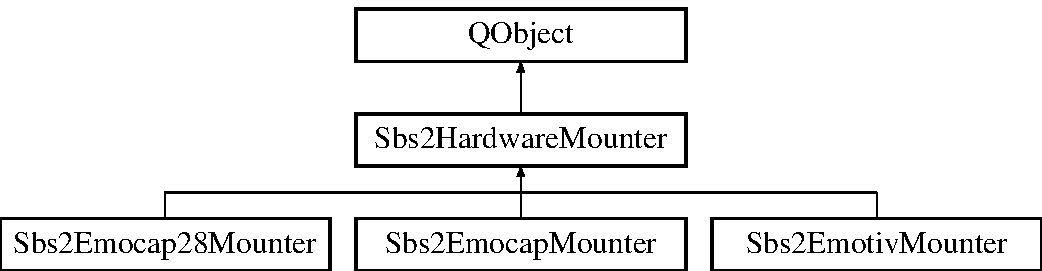
\includegraphics[height=3.000000cm]{classSbs2HardwareMounter}
\end{center}
\end{figure}
\subsection*{Public Slots}
\begin{DoxyCompactItemize}
\item 
virtual void \hyperlink{classSbs2HardwareMounter_a5a37fde350e3db7bf70d7be368b876e9}{start} ()=0
\item 
virtual void \hyperlink{classSbs2HardwareMounter_a27bc12c9e5a1eeeed3669bc6afd780dd}{stop} ()=0
\item 
virtual void \hyperlink{classSbs2HardwareMounter_ae890d839cf616daf0ea80cc2e44ce2bd}{invalidate} ()=0
\end{DoxyCompactItemize}
\subsection*{Signals}
\begin{DoxyCompactItemize}
\item 
void \hyperlink{classSbs2HardwareMounter_a42bb432337e0cffc85baadf83a1813cd}{device\-Found} (Q\-Map$<$ Q\-String, Q\-Variant $>$ params)
\item 
void \hyperlink{classSbs2HardwareMounter_a715feed025039fbf3aaba0cb0621b453}{device\-Lost} ()
\end{DoxyCompactItemize}
\subsection*{Public Member Functions}
\begin{DoxyCompactItemize}
\item 
\hyperlink{classSbs2HardwareMounter_a791fa95ec691263fc0fdf1bddd21e92a}{$\sim$\-Sbs2\-Hardware\-Mounter} ()
\end{DoxyCompactItemize}
\subsection*{Static Public Member Functions}
\begin{DoxyCompactItemize}
\item 
static Q\-String \hyperlink{classSbs2HardwareMounter_ae859631cf871c19b0b1163f26eacde4f}{get\-Identifier} ()
\end{DoxyCompactItemize}
\subsection*{Protected Member Functions}
\begin{DoxyCompactItemize}
\item 
\hyperlink{classSbs2HardwareMounter_a0b57bd594cc2519164ca079580937181}{Sbs2\-Hardware\-Mounter} (Q\-Object $\ast$parent=0)
\item 
void \hyperlink{classSbs2HardwareMounter_ac2129b6eb23d4eddcc9b388dee96ba18}{my\-Sleep} ()
\item 
virtual void \hyperlink{classSbs2HardwareMounter_aa6be696873d18aea5c5e27d6ff92105d}{init} ()
\item 
virtual void \hyperlink{classSbs2HardwareMounter_af6c3fc37fa15ecadcf968d6ffcae0ec6}{mount} ()
\item 
virtual void \hyperlink{classSbs2HardwareMounter_ae248c626ae5bf0d7a73550e859d96190}{umount} ()
\item 
virtual void \hyperlink{classSbs2HardwareMounter_a73ed9f3ddf38747263ca040f5e433270}{read\-Hardware\-Parameters} ()
\end{DoxyCompactItemize}
\subsection*{Static Protected Attributes}
\begin{DoxyCompactItemize}
\item 
static Q\-String \hyperlink{classSbs2HardwareMounter_a84df0b714f439793b05c23244b88fa4d}{mounted\-Hardware} = \char`\"{}\char`\"{}
\item 
static Q\-String \hyperlink{classSbs2HardwareMounter_a00ac9b3100310ddf9615116c8d33af9c}{identifier} = \char`\"{}\char`\"{}
\end{DoxyCompactItemize}


\subsection{Detailed Description}
Smartphone Brain Scanner 2 License Agreement (M\-I\-T License)

Copyright (c) 2012 Arkadiusz Stopczynski, Jakob Eg Larsen, Carsten Stahlhut, Michael Kai Petersen, Lars Kai Hansen. Technical University of Denmark, \hyperlink{namespaceDTU}{D\-T\-U} Informatics, Cognitive Systems Section. \href{http://code.google.com/p/smartphonebrainscanner2}{\tt http\-://code.\-google.\-com/p/smartphonebrainscanner2}

Permission is hereby granted, free of charge, to any person obtaining a copy of this software and associated documentation files (the \char`\"{}\-Software\char`\"{}), to deal in the Software without restriction, including without limitation the rights to use, copy, modify, merge, publish, distribute, sublicense, and/or sell copies of the Software, and to permit persons to whom the Software is furnished to do so, subject to the following conditions\-:

The above copyright notice and this permission notice shall be included in all copies or substantial portions of the Software.

T\-H\-E S\-O\-F\-T\-W\-A\-R\-E I\-S P\-R\-O\-V\-I\-D\-E\-D \char`\"{}\-A\-S I\-S\char`\"{}, W\-I\-T\-H\-O\-U\-T W\-A\-R\-R\-A\-N\-T\-Y O\-F A\-N\-Y K\-I\-N\-D, E\-X\-P\-R\-E\-S\-S O\-R I\-M\-P\-L\-I\-E\-D, I\-N\-C\-L\-U\-D\-I\-N\-G B\-U\-T N\-O\-T L\-I\-M\-I\-T\-E\-D T\-O T\-H\-E W\-A\-R\-R\-A\-N\-T\-I\-E\-S O\-F M\-E\-R\-C\-H\-A\-N\-T\-A\-B\-I\-L\-I\-T\-Y, F\-I\-T\-N\-E\-S\-S F\-O\-R A P\-A\-R\-T\-I\-C\-U\-L\-A\-R P\-U\-R\-P\-O\-S\-E A\-N\-D N\-O\-N\-I\-N\-F\-R\-I\-N\-G\-E\-M\-E\-N\-T. I\-N N\-O E\-V\-E\-N\-T S\-H\-A\-L\-L T\-H\-E A\-U\-T\-H\-O\-R\-S O\-R C\-O\-P\-Y\-R\-I\-G\-H\-T H\-O\-L\-D\-E\-R\-S B\-E L\-I\-A\-B\-L\-E F\-O\-R A\-N\-Y C\-L\-A\-I\-M, D\-A\-M\-A\-G\-E\-S O\-R O\-T\-H\-E\-R L\-I\-A\-B\-I\-L\-I\-T\-Y, W\-H\-E\-T\-H\-E\-R I\-N A\-N A\-C\-T\-I\-O\-N O\-F C\-O\-N\-T\-R\-A\-C\-T, T\-O\-R\-T O\-R O\-T\-H\-E\-R\-W\-I\-S\-E, A\-R\-I\-S\-I\-N\-G F\-R\-O\-M, O\-U\-T O\-F O\-R I\-N C\-O\-N\-N\-E\-C\-T\-I\-O\-N W\-I\-T\-H T\-H\-E S\-O\-F\-T\-W\-A\-R\-E O\-R T\-H\-E U\-S\-E O\-R O\-T\-H\-E\-R D\-E\-A\-L\-I\-N\-G\-S I\-N T\-H\-E S\-O\-F\-T\-W\-A\-R\-E. 

\subsection{Constructor \& Destructor Documentation}
\hypertarget{classSbs2HardwareMounter_a791fa95ec691263fc0fdf1bddd21e92a}{\index{Sbs2\-Hardware\-Mounter@{Sbs2\-Hardware\-Mounter}!$\sim$\-Sbs2\-Hardware\-Mounter@{$\sim$\-Sbs2\-Hardware\-Mounter}}
\index{$\sim$\-Sbs2\-Hardware\-Mounter@{$\sim$\-Sbs2\-Hardware\-Mounter}!Sbs2HardwareMounter@{Sbs2\-Hardware\-Mounter}}
\subsubsection[{$\sim$\-Sbs2\-Hardware\-Mounter}]{\setlength{\rightskip}{0pt plus 5cm}Sbs2\-Hardware\-Mounter\-::$\sim$\-Sbs2\-Hardware\-Mounter (
\begin{DoxyParamCaption}
{}
\end{DoxyParamCaption}
)}}\label{classSbs2HardwareMounter_a791fa95ec691263fc0fdf1bddd21e92a}
\hypertarget{classSbs2HardwareMounter_a0b57bd594cc2519164ca079580937181}{\index{Sbs2\-Hardware\-Mounter@{Sbs2\-Hardware\-Mounter}!Sbs2\-Hardware\-Mounter@{Sbs2\-Hardware\-Mounter}}
\index{Sbs2\-Hardware\-Mounter@{Sbs2\-Hardware\-Mounter}!Sbs2HardwareMounter@{Sbs2\-Hardware\-Mounter}}
\subsubsection[{Sbs2\-Hardware\-Mounter}]{\setlength{\rightskip}{0pt plus 5cm}Sbs2\-Hardware\-Mounter\-::\-Sbs2\-Hardware\-Mounter (
\begin{DoxyParamCaption}
\item[{Q\-Object $\ast$}]{parent = {\ttfamily 0}}
\end{DoxyParamCaption}
)\hspace{0.3cm}{\ttfamily [protected]}}}\label{classSbs2HardwareMounter_a0b57bd594cc2519164ca079580937181}


\subsection{Member Function Documentation}
\hypertarget{classSbs2HardwareMounter_a42bb432337e0cffc85baadf83a1813cd}{\index{Sbs2\-Hardware\-Mounter@{Sbs2\-Hardware\-Mounter}!device\-Found@{device\-Found}}
\index{device\-Found@{device\-Found}!Sbs2HardwareMounter@{Sbs2\-Hardware\-Mounter}}
\subsubsection[{device\-Found}]{\setlength{\rightskip}{0pt plus 5cm}void Sbs2\-Hardware\-Mounter\-::device\-Found (
\begin{DoxyParamCaption}
\item[{Q\-Map$<$ Q\-String, Q\-Variant $>$}]{params}
\end{DoxyParamCaption}
)\hspace{0.3cm}{\ttfamily [signal]}}}\label{classSbs2HardwareMounter_a42bb432337e0cffc85baadf83a1813cd}
\hypertarget{classSbs2HardwareMounter_a715feed025039fbf3aaba0cb0621b453}{\index{Sbs2\-Hardware\-Mounter@{Sbs2\-Hardware\-Mounter}!device\-Lost@{device\-Lost}}
\index{device\-Lost@{device\-Lost}!Sbs2HardwareMounter@{Sbs2\-Hardware\-Mounter}}
\subsubsection[{device\-Lost}]{\setlength{\rightskip}{0pt plus 5cm}void Sbs2\-Hardware\-Mounter\-::device\-Lost (
\begin{DoxyParamCaption}
{}
\end{DoxyParamCaption}
)\hspace{0.3cm}{\ttfamily [signal]}}}\label{classSbs2HardwareMounter_a715feed025039fbf3aaba0cb0621b453}
\hypertarget{classSbs2HardwareMounter_ae859631cf871c19b0b1163f26eacde4f}{\index{Sbs2\-Hardware\-Mounter@{Sbs2\-Hardware\-Mounter}!get\-Identifier@{get\-Identifier}}
\index{get\-Identifier@{get\-Identifier}!Sbs2HardwareMounter@{Sbs2\-Hardware\-Mounter}}
\subsubsection[{get\-Identifier}]{\setlength{\rightskip}{0pt plus 5cm}Q\-String Sbs2\-Hardware\-Mounter\-::get\-Identifier (
\begin{DoxyParamCaption}
{}
\end{DoxyParamCaption}
)\hspace{0.3cm}{\ttfamily [static]}}}\label{classSbs2HardwareMounter_ae859631cf871c19b0b1163f26eacde4f}
\hypertarget{classSbs2HardwareMounter_aa6be696873d18aea5c5e27d6ff92105d}{\index{Sbs2\-Hardware\-Mounter@{Sbs2\-Hardware\-Mounter}!init@{init}}
\index{init@{init}!Sbs2HardwareMounter@{Sbs2\-Hardware\-Mounter}}
\subsubsection[{init}]{\setlength{\rightskip}{0pt plus 5cm}void Sbs2\-Hardware\-Mounter\-::init (
\begin{DoxyParamCaption}
{}
\end{DoxyParamCaption}
)\hspace{0.3cm}{\ttfamily [protected]}, {\ttfamily [virtual]}}}\label{classSbs2HardwareMounter_aa6be696873d18aea5c5e27d6ff92105d}
\hypertarget{classSbs2HardwareMounter_ae890d839cf616daf0ea80cc2e44ce2bd}{\index{Sbs2\-Hardware\-Mounter@{Sbs2\-Hardware\-Mounter}!invalidate@{invalidate}}
\index{invalidate@{invalidate}!Sbs2HardwareMounter@{Sbs2\-Hardware\-Mounter}}
\subsubsection[{invalidate}]{\setlength{\rightskip}{0pt plus 5cm}virtual void Sbs2\-Hardware\-Mounter\-::invalidate (
\begin{DoxyParamCaption}
{}
\end{DoxyParamCaption}
)\hspace{0.3cm}{\ttfamily [pure virtual]}, {\ttfamily [slot]}}}\label{classSbs2HardwareMounter_ae890d839cf616daf0ea80cc2e44ce2bd}
\hypertarget{classSbs2HardwareMounter_af6c3fc37fa15ecadcf968d6ffcae0ec6}{\index{Sbs2\-Hardware\-Mounter@{Sbs2\-Hardware\-Mounter}!mount@{mount}}
\index{mount@{mount}!Sbs2HardwareMounter@{Sbs2\-Hardware\-Mounter}}
\subsubsection[{mount}]{\setlength{\rightskip}{0pt plus 5cm}void Sbs2\-Hardware\-Mounter\-::mount (
\begin{DoxyParamCaption}
{}
\end{DoxyParamCaption}
)\hspace{0.3cm}{\ttfamily [protected]}, {\ttfamily [virtual]}}}\label{classSbs2HardwareMounter_af6c3fc37fa15ecadcf968d6ffcae0ec6}
\hypertarget{classSbs2HardwareMounter_ac2129b6eb23d4eddcc9b388dee96ba18}{\index{Sbs2\-Hardware\-Mounter@{Sbs2\-Hardware\-Mounter}!my\-Sleep@{my\-Sleep}}
\index{my\-Sleep@{my\-Sleep}!Sbs2HardwareMounter@{Sbs2\-Hardware\-Mounter}}
\subsubsection[{my\-Sleep}]{\setlength{\rightskip}{0pt plus 5cm}void Sbs2\-Hardware\-Mounter\-::my\-Sleep (
\begin{DoxyParamCaption}
{}
\end{DoxyParamCaption}
)\hspace{0.3cm}{\ttfamily [protected]}}}\label{classSbs2HardwareMounter_ac2129b6eb23d4eddcc9b388dee96ba18}
\hypertarget{classSbs2HardwareMounter_a73ed9f3ddf38747263ca040f5e433270}{\index{Sbs2\-Hardware\-Mounter@{Sbs2\-Hardware\-Mounter}!read\-Hardware\-Parameters@{read\-Hardware\-Parameters}}
\index{read\-Hardware\-Parameters@{read\-Hardware\-Parameters}!Sbs2HardwareMounter@{Sbs2\-Hardware\-Mounter}}
\subsubsection[{read\-Hardware\-Parameters}]{\setlength{\rightskip}{0pt plus 5cm}void Sbs2\-Hardware\-Mounter\-::read\-Hardware\-Parameters (
\begin{DoxyParamCaption}
{}
\end{DoxyParamCaption}
)\hspace{0.3cm}{\ttfamily [protected]}, {\ttfamily [virtual]}}}\label{classSbs2HardwareMounter_a73ed9f3ddf38747263ca040f5e433270}
\hypertarget{classSbs2HardwareMounter_a5a37fde350e3db7bf70d7be368b876e9}{\index{Sbs2\-Hardware\-Mounter@{Sbs2\-Hardware\-Mounter}!start@{start}}
\index{start@{start}!Sbs2HardwareMounter@{Sbs2\-Hardware\-Mounter}}
\subsubsection[{start}]{\setlength{\rightskip}{0pt plus 5cm}void Sbs2\-Hardware\-Mounter\-::start (
\begin{DoxyParamCaption}
{}
\end{DoxyParamCaption}
)\hspace{0.3cm}{\ttfamily [pure virtual]}, {\ttfamily [slot]}}}\label{classSbs2HardwareMounter_a5a37fde350e3db7bf70d7be368b876e9}
\hypertarget{classSbs2HardwareMounter_a27bc12c9e5a1eeeed3669bc6afd780dd}{\index{Sbs2\-Hardware\-Mounter@{Sbs2\-Hardware\-Mounter}!stop@{stop}}
\index{stop@{stop}!Sbs2HardwareMounter@{Sbs2\-Hardware\-Mounter}}
\subsubsection[{stop}]{\setlength{\rightskip}{0pt plus 5cm}virtual void Sbs2\-Hardware\-Mounter\-::stop (
\begin{DoxyParamCaption}
{}
\end{DoxyParamCaption}
)\hspace{0.3cm}{\ttfamily [pure virtual]}, {\ttfamily [slot]}}}\label{classSbs2HardwareMounter_a27bc12c9e5a1eeeed3669bc6afd780dd}
\hypertarget{classSbs2HardwareMounter_ae248c626ae5bf0d7a73550e859d96190}{\index{Sbs2\-Hardware\-Mounter@{Sbs2\-Hardware\-Mounter}!umount@{umount}}
\index{umount@{umount}!Sbs2HardwareMounter@{Sbs2\-Hardware\-Mounter}}
\subsubsection[{umount}]{\setlength{\rightskip}{0pt plus 5cm}void Sbs2\-Hardware\-Mounter\-::umount (
\begin{DoxyParamCaption}
{}
\end{DoxyParamCaption}
)\hspace{0.3cm}{\ttfamily [protected]}, {\ttfamily [virtual]}}}\label{classSbs2HardwareMounter_ae248c626ae5bf0d7a73550e859d96190}


\subsection{Member Data Documentation}
\hypertarget{classSbs2HardwareMounter_a00ac9b3100310ddf9615116c8d33af9c}{\index{Sbs2\-Hardware\-Mounter@{Sbs2\-Hardware\-Mounter}!identifier@{identifier}}
\index{identifier@{identifier}!Sbs2HardwareMounter@{Sbs2\-Hardware\-Mounter}}
\subsubsection[{identifier}]{\setlength{\rightskip}{0pt plus 5cm}Q\-String Sbs2\-Hardware\-Mounter\-::identifier = \char`\"{}\char`\"{}\hspace{0.3cm}{\ttfamily [static]}, {\ttfamily [protected]}}}\label{classSbs2HardwareMounter_a00ac9b3100310ddf9615116c8d33af9c}
\hypertarget{classSbs2HardwareMounter_a84df0b714f439793b05c23244b88fa4d}{\index{Sbs2\-Hardware\-Mounter@{Sbs2\-Hardware\-Mounter}!mounted\-Hardware@{mounted\-Hardware}}
\index{mounted\-Hardware@{mounted\-Hardware}!Sbs2HardwareMounter@{Sbs2\-Hardware\-Mounter}}
\subsubsection[{mounted\-Hardware}]{\setlength{\rightskip}{0pt plus 5cm}Q\-String Sbs2\-Hardware\-Mounter\-::mounted\-Hardware = \char`\"{}\char`\"{}\hspace{0.3cm}{\ttfamily [static]}, {\ttfamily [protected]}}}\label{classSbs2HardwareMounter_a84df0b714f439793b05c23244b88fa4d}


The documentation for this class was generated from the following files\-:\begin{DoxyCompactItemize}
\item 
/media/philipjhj/\-Data/\-One\-Drive/\-Studie/\-Studenterprogrammør/\-S\-B\-S3/smartphonebrainscanner2-\/core/src/hardware/\hyperlink{sbs2hardwaremounter_8h}{sbs2hardwaremounter.\-h}\item 
/media/philipjhj/\-Data/\-One\-Drive/\-Studie/\-Studenterprogrammør/\-S\-B\-S3/smartphonebrainscanner2-\/core/src/hardware/\hyperlink{sbs2hardwaremounter_8cpp}{sbs2hardwaremounter.\-cpp}\end{DoxyCompactItemize}

\hypertarget{classSbs2NetworkHandler}{\section{Sbs2\-Network\-Handler Class Reference}
\label{classSbs2NetworkHandler}\index{Sbs2\-Network\-Handler@{Sbs2\-Network\-Handler}}
}


{\ttfamily \#include $<$sbs2networkhandler.\-h$>$}

Inheritance diagram for Sbs2\-Network\-Handler\-:\begin{figure}[H]
\begin{center}
\leavevmode
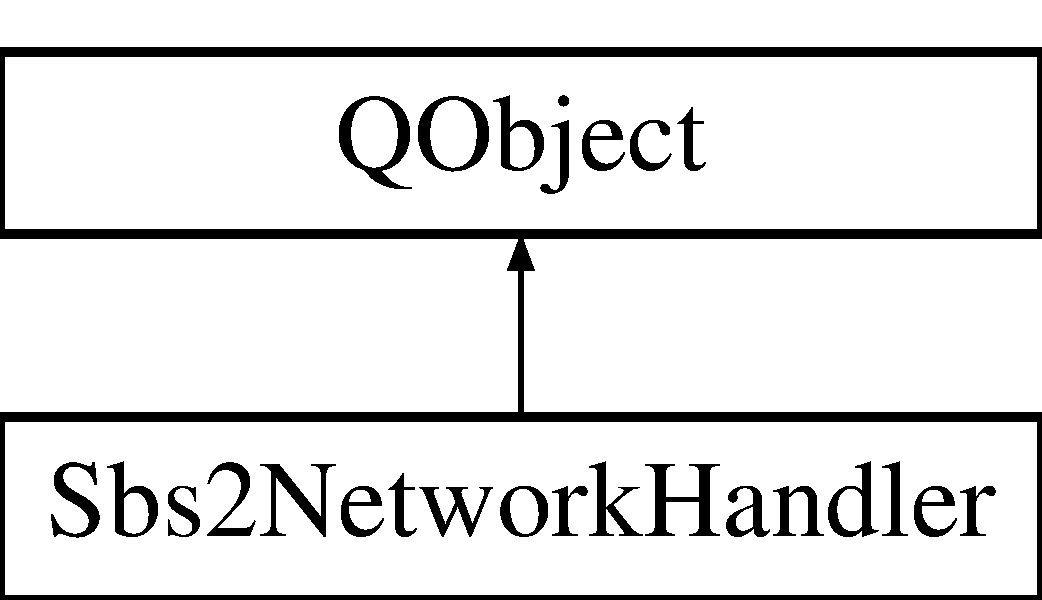
\includegraphics[height=2.000000cm]{classSbs2NetworkHandler}
\end{center}
\end{figure}
\subsection*{Public Slots}
\begin{DoxyCompactItemize}
\item 
void \hyperlink{classSbs2NetworkHandler_a442ac8b20364e99764921ccfcee133a5}{turn\-Send\-Raw\-Data\-On} (Q\-String raw\-Data\-Server\-Address\-\_\-, int raw\-Data\-Port\-\_\-, int raw\-Data\-Size\-\_\-, int raw\-Data\-Queue\-Length\-\_\-)
\item 
void \hyperlink{classSbs2NetworkHandler_aa2af80c37111b3fdfa2c45b0194d1b02}{turn\-Send\-Raw\-Data\-Off} ()
\item 
void \hyperlink{classSbs2NetworkHandler_a88a1d746fd4eec22f393964fea5e5a11}{add\-Raw\-Data\-Host} (Q\-String address, int port)
\item 
void \hyperlink{classSbs2NetworkHandler_aded95af0fab1947e3a2c6e09d02f3464}{remove\-Raw\-Data\-Host} (Q\-String address, int port)
\item 
void \hyperlink{classSbs2NetworkHandler_a450fb80b4be000f8768c0c8b0e14e5c1}{send\-Raw\-Data} (char $\ast$data)
\item 
void \hyperlink{classSbs2NetworkHandler_a71d931b6624b6811992117db7d07d86c}{turn\-Receive\-Raw\-Data\-On} (Q\-String raw\-Data\-Udp\-Input\-Address\-\_\-, int raw\-Data\-Udp\-Input\-Port\-\_\-)
\item 
void \hyperlink{classSbs2NetworkHandler_a7a442ffbe3784b619645f773f11b5415}{turn\-Receive\-Raw\-Data\-Off} ()
\item 
void \hyperlink{classSbs2NetworkHandler_a7c894803abb0cf6066d324434614e59e}{read\-Raw\-Data} ()
\item 
void \hyperlink{classSbs2NetworkHandler_aaef038ae07bba835f767f525024885de}{send\-Message} (Q\-String message, Q\-String address, int port)
\item 
void \hyperlink{classSbs2NetworkHandler_a5859053ca998f4cbfccec0110417f3aa}{send\-Message} (Q\-String message)
\item 
void \hyperlink{classSbs2NetworkHandler_afffcfd11f6d08aeb0715414f1023ca31}{add\-Message\-Udp\-Output\-Host} (Q\-String address, int port)
\item 
void \hyperlink{classSbs2NetworkHandler_a55b23c60e565a927e18e53b8163a6867}{remove\-Message\-Udp\-Output\-Host} (Q\-String address)
\item 
void \hyperlink{classSbs2NetworkHandler_a11cf3eba00cda5a186318fc1ebe0b5f8}{clear\-Message\-Udp\-Output\-Hosts} ()
\item 
void \hyperlink{classSbs2NetworkHandler_a702a02dcef9a5c35a6964e40a434b1d0}{turn\-Receive\-Message\-On} (Q\-String address, int port)
\item 
void \hyperlink{classSbs2NetworkHandler_a698d27f3ed1efe4c7c050b764a3e98ac}{turn\-Receive\-Message\-Off} ()
\item 
void \hyperlink{classSbs2NetworkHandler_afeb3b4208880d2a902aa77dc02876773}{read\-Message} ()
\end{DoxyCompactItemize}
\subsection*{Signals}
\begin{DoxyCompactItemize}
\item 
void \hyperlink{classSbs2NetworkHandler_a327df0610ce097b253e77d1d14d2a989}{raw\-Data\-Sent\-Signal} ()
\item 
void \hyperlink{classSbs2NetworkHandler_ac86bb75fedf2d2c158450863880fd9b3}{raw\-Data\-Received} (char $\ast$data, int size, Q\-String address, int port)
\item 
void \hyperlink{classSbs2NetworkHandler_aab0443a2be25f984e927979d51fd2f04}{raw\-Data\-Received} (Q\-Vector$<$ char $\ast$ $>$ $\ast$data, int counter)
\item 
void \hyperlink{classSbs2NetworkHandler_a369d51a13840755c33e870770aa7465f}{raw\-Data\-Received} (Q\-Udp\-Socket $\ast$raw\-Data\-Udp\-Input\-Socket)
\item 
void \hyperlink{classSbs2NetworkHandler_a9eef01f06126c5a2468f604dfb7a466c}{message\-Received} (Q\-String data, Q\-String sender, int sender\-Port)
\end{DoxyCompactItemize}
\subsection*{Public Member Functions}
\begin{DoxyCompactItemize}
\item 
\hyperlink{classSbs2NetworkHandler_a62a07c2d8e97abdf19b531b672327cdd}{Sbs2\-Network\-Handler} (Q\-Object $\ast$parent=0)
\end{DoxyCompactItemize}


\subsection{Constructor \& Destructor Documentation}
\hypertarget{classSbs2NetworkHandler_a62a07c2d8e97abdf19b531b672327cdd}{\index{Sbs2\-Network\-Handler@{Sbs2\-Network\-Handler}!Sbs2\-Network\-Handler@{Sbs2\-Network\-Handler}}
\index{Sbs2\-Network\-Handler@{Sbs2\-Network\-Handler}!Sbs2NetworkHandler@{Sbs2\-Network\-Handler}}
\subsubsection[{Sbs2\-Network\-Handler}]{\setlength{\rightskip}{0pt plus 5cm}Sbs2\-Network\-Handler\-::\-Sbs2\-Network\-Handler (
\begin{DoxyParamCaption}
\item[{Q\-Object $\ast$}]{parent = {\ttfamily 0}}
\end{DoxyParamCaption}
)}}\label{classSbs2NetworkHandler_a62a07c2d8e97abdf19b531b672327cdd}


\subsection{Member Function Documentation}
\hypertarget{classSbs2NetworkHandler_afffcfd11f6d08aeb0715414f1023ca31}{\index{Sbs2\-Network\-Handler@{Sbs2\-Network\-Handler}!add\-Message\-Udp\-Output\-Host@{add\-Message\-Udp\-Output\-Host}}
\index{add\-Message\-Udp\-Output\-Host@{add\-Message\-Udp\-Output\-Host}!Sbs2NetworkHandler@{Sbs2\-Network\-Handler}}
\subsubsection[{add\-Message\-Udp\-Output\-Host}]{\setlength{\rightskip}{0pt plus 5cm}void Sbs2\-Network\-Handler\-::add\-Message\-Udp\-Output\-Host (
\begin{DoxyParamCaption}
\item[{Q\-String}]{address, }
\item[{int}]{port}
\end{DoxyParamCaption}
)\hspace{0.3cm}{\ttfamily [slot]}}}\label{classSbs2NetworkHandler_afffcfd11f6d08aeb0715414f1023ca31}
\hypertarget{classSbs2NetworkHandler_a88a1d746fd4eec22f393964fea5e5a11}{\index{Sbs2\-Network\-Handler@{Sbs2\-Network\-Handler}!add\-Raw\-Data\-Host@{add\-Raw\-Data\-Host}}
\index{add\-Raw\-Data\-Host@{add\-Raw\-Data\-Host}!Sbs2NetworkHandler@{Sbs2\-Network\-Handler}}
\subsubsection[{add\-Raw\-Data\-Host}]{\setlength{\rightskip}{0pt plus 5cm}void Sbs2\-Network\-Handler\-::add\-Raw\-Data\-Host (
\begin{DoxyParamCaption}
\item[{Q\-String}]{address, }
\item[{int}]{port}
\end{DoxyParamCaption}
)\hspace{0.3cm}{\ttfamily [slot]}}}\label{classSbs2NetworkHandler_a88a1d746fd4eec22f393964fea5e5a11}
\hypertarget{classSbs2NetworkHandler_a11cf3eba00cda5a186318fc1ebe0b5f8}{\index{Sbs2\-Network\-Handler@{Sbs2\-Network\-Handler}!clear\-Message\-Udp\-Output\-Hosts@{clear\-Message\-Udp\-Output\-Hosts}}
\index{clear\-Message\-Udp\-Output\-Hosts@{clear\-Message\-Udp\-Output\-Hosts}!Sbs2NetworkHandler@{Sbs2\-Network\-Handler}}
\subsubsection[{clear\-Message\-Udp\-Output\-Hosts}]{\setlength{\rightskip}{0pt plus 5cm}void Sbs2\-Network\-Handler\-::clear\-Message\-Udp\-Output\-Hosts (
\begin{DoxyParamCaption}
{}
\end{DoxyParamCaption}
)\hspace{0.3cm}{\ttfamily [slot]}}}\label{classSbs2NetworkHandler_a11cf3eba00cda5a186318fc1ebe0b5f8}
\hypertarget{classSbs2NetworkHandler_a9eef01f06126c5a2468f604dfb7a466c}{\index{Sbs2\-Network\-Handler@{Sbs2\-Network\-Handler}!message\-Received@{message\-Received}}
\index{message\-Received@{message\-Received}!Sbs2NetworkHandler@{Sbs2\-Network\-Handler}}
\subsubsection[{message\-Received}]{\setlength{\rightskip}{0pt plus 5cm}void Sbs2\-Network\-Handler\-::message\-Received (
\begin{DoxyParamCaption}
\item[{Q\-String}]{data, }
\item[{Q\-String}]{sender, }
\item[{int}]{sender\-Port}
\end{DoxyParamCaption}
)\hspace{0.3cm}{\ttfamily [signal]}}}\label{classSbs2NetworkHandler_a9eef01f06126c5a2468f604dfb7a466c}
\hypertarget{classSbs2NetworkHandler_ac86bb75fedf2d2c158450863880fd9b3}{\index{Sbs2\-Network\-Handler@{Sbs2\-Network\-Handler}!raw\-Data\-Received@{raw\-Data\-Received}}
\index{raw\-Data\-Received@{raw\-Data\-Received}!Sbs2NetworkHandler@{Sbs2\-Network\-Handler}}
\subsubsection[{raw\-Data\-Received}]{\setlength{\rightskip}{0pt plus 5cm}void Sbs2\-Network\-Handler\-::raw\-Data\-Received (
\begin{DoxyParamCaption}
\item[{char $\ast$}]{data, }
\item[{int}]{size, }
\item[{Q\-String}]{address, }
\item[{int}]{port}
\end{DoxyParamCaption}
)\hspace{0.3cm}{\ttfamily [signal]}}}\label{classSbs2NetworkHandler_ac86bb75fedf2d2c158450863880fd9b3}
\hypertarget{classSbs2NetworkHandler_aab0443a2be25f984e927979d51fd2f04}{\index{Sbs2\-Network\-Handler@{Sbs2\-Network\-Handler}!raw\-Data\-Received@{raw\-Data\-Received}}
\index{raw\-Data\-Received@{raw\-Data\-Received}!Sbs2NetworkHandler@{Sbs2\-Network\-Handler}}
\subsubsection[{raw\-Data\-Received}]{\setlength{\rightskip}{0pt plus 5cm}void Sbs2\-Network\-Handler\-::raw\-Data\-Received (
\begin{DoxyParamCaption}
\item[{Q\-Vector$<$ char $\ast$ $>$ $\ast$}]{data, }
\item[{int}]{counter}
\end{DoxyParamCaption}
)\hspace{0.3cm}{\ttfamily [signal]}}}\label{classSbs2NetworkHandler_aab0443a2be25f984e927979d51fd2f04}
\hypertarget{classSbs2NetworkHandler_a369d51a13840755c33e870770aa7465f}{\index{Sbs2\-Network\-Handler@{Sbs2\-Network\-Handler}!raw\-Data\-Received@{raw\-Data\-Received}}
\index{raw\-Data\-Received@{raw\-Data\-Received}!Sbs2NetworkHandler@{Sbs2\-Network\-Handler}}
\subsubsection[{raw\-Data\-Received}]{\setlength{\rightskip}{0pt plus 5cm}void Sbs2\-Network\-Handler\-::raw\-Data\-Received (
\begin{DoxyParamCaption}
\item[{Q\-Udp\-Socket $\ast$}]{raw\-Data\-Udp\-Input\-Socket}
\end{DoxyParamCaption}
)\hspace{0.3cm}{\ttfamily [signal]}}}\label{classSbs2NetworkHandler_a369d51a13840755c33e870770aa7465f}
\hypertarget{classSbs2NetworkHandler_a327df0610ce097b253e77d1d14d2a989}{\index{Sbs2\-Network\-Handler@{Sbs2\-Network\-Handler}!raw\-Data\-Sent\-Signal@{raw\-Data\-Sent\-Signal}}
\index{raw\-Data\-Sent\-Signal@{raw\-Data\-Sent\-Signal}!Sbs2NetworkHandler@{Sbs2\-Network\-Handler}}
\subsubsection[{raw\-Data\-Sent\-Signal}]{\setlength{\rightskip}{0pt plus 5cm}void Sbs2\-Network\-Handler\-::raw\-Data\-Sent\-Signal (
\begin{DoxyParamCaption}
{}
\end{DoxyParamCaption}
)\hspace{0.3cm}{\ttfamily [signal]}}}\label{classSbs2NetworkHandler_a327df0610ce097b253e77d1d14d2a989}
\hypertarget{classSbs2NetworkHandler_afeb3b4208880d2a902aa77dc02876773}{\index{Sbs2\-Network\-Handler@{Sbs2\-Network\-Handler}!read\-Message@{read\-Message}}
\index{read\-Message@{read\-Message}!Sbs2NetworkHandler@{Sbs2\-Network\-Handler}}
\subsubsection[{read\-Message}]{\setlength{\rightskip}{0pt plus 5cm}void Sbs2\-Network\-Handler\-::read\-Message (
\begin{DoxyParamCaption}
{}
\end{DoxyParamCaption}
)\hspace{0.3cm}{\ttfamily [slot]}}}\label{classSbs2NetworkHandler_afeb3b4208880d2a902aa77dc02876773}
\hypertarget{classSbs2NetworkHandler_a7c894803abb0cf6066d324434614e59e}{\index{Sbs2\-Network\-Handler@{Sbs2\-Network\-Handler}!read\-Raw\-Data@{read\-Raw\-Data}}
\index{read\-Raw\-Data@{read\-Raw\-Data}!Sbs2NetworkHandler@{Sbs2\-Network\-Handler}}
\subsubsection[{read\-Raw\-Data}]{\setlength{\rightskip}{0pt plus 5cm}void Sbs2\-Network\-Handler\-::read\-Raw\-Data (
\begin{DoxyParamCaption}
{}
\end{DoxyParamCaption}
)\hspace{0.3cm}{\ttfamily [slot]}}}\label{classSbs2NetworkHandler_a7c894803abb0cf6066d324434614e59e}
\hypertarget{classSbs2NetworkHandler_a55b23c60e565a927e18e53b8163a6867}{\index{Sbs2\-Network\-Handler@{Sbs2\-Network\-Handler}!remove\-Message\-Udp\-Output\-Host@{remove\-Message\-Udp\-Output\-Host}}
\index{remove\-Message\-Udp\-Output\-Host@{remove\-Message\-Udp\-Output\-Host}!Sbs2NetworkHandler@{Sbs2\-Network\-Handler}}
\subsubsection[{remove\-Message\-Udp\-Output\-Host}]{\setlength{\rightskip}{0pt plus 5cm}void Sbs2\-Network\-Handler\-::remove\-Message\-Udp\-Output\-Host (
\begin{DoxyParamCaption}
\item[{Q\-String}]{address}
\end{DoxyParamCaption}
)\hspace{0.3cm}{\ttfamily [slot]}}}\label{classSbs2NetworkHandler_a55b23c60e565a927e18e53b8163a6867}
\hypertarget{classSbs2NetworkHandler_aded95af0fab1947e3a2c6e09d02f3464}{\index{Sbs2\-Network\-Handler@{Sbs2\-Network\-Handler}!remove\-Raw\-Data\-Host@{remove\-Raw\-Data\-Host}}
\index{remove\-Raw\-Data\-Host@{remove\-Raw\-Data\-Host}!Sbs2NetworkHandler@{Sbs2\-Network\-Handler}}
\subsubsection[{remove\-Raw\-Data\-Host}]{\setlength{\rightskip}{0pt plus 5cm}void Sbs2\-Network\-Handler\-::remove\-Raw\-Data\-Host (
\begin{DoxyParamCaption}
\item[{Q\-String}]{address, }
\item[{int}]{port}
\end{DoxyParamCaption}
)\hspace{0.3cm}{\ttfamily [slot]}}}\label{classSbs2NetworkHandler_aded95af0fab1947e3a2c6e09d02f3464}
\hypertarget{classSbs2NetworkHandler_aaef038ae07bba835f767f525024885de}{\index{Sbs2\-Network\-Handler@{Sbs2\-Network\-Handler}!send\-Message@{send\-Message}}
\index{send\-Message@{send\-Message}!Sbs2NetworkHandler@{Sbs2\-Network\-Handler}}
\subsubsection[{send\-Message}]{\setlength{\rightskip}{0pt plus 5cm}void Sbs2\-Network\-Handler\-::send\-Message (
\begin{DoxyParamCaption}
\item[{Q\-String}]{message, }
\item[{Q\-String}]{address, }
\item[{int}]{port}
\end{DoxyParamCaption}
)\hspace{0.3cm}{\ttfamily [slot]}}}\label{classSbs2NetworkHandler_aaef038ae07bba835f767f525024885de}
\hypertarget{classSbs2NetworkHandler_a5859053ca998f4cbfccec0110417f3aa}{\index{Sbs2\-Network\-Handler@{Sbs2\-Network\-Handler}!send\-Message@{send\-Message}}
\index{send\-Message@{send\-Message}!Sbs2NetworkHandler@{Sbs2\-Network\-Handler}}
\subsubsection[{send\-Message}]{\setlength{\rightskip}{0pt plus 5cm}void Sbs2\-Network\-Handler\-::send\-Message (
\begin{DoxyParamCaption}
\item[{Q\-String}]{message}
\end{DoxyParamCaption}
)\hspace{0.3cm}{\ttfamily [slot]}}}\label{classSbs2NetworkHandler_a5859053ca998f4cbfccec0110417f3aa}
\hypertarget{classSbs2NetworkHandler_a450fb80b4be000f8768c0c8b0e14e5c1}{\index{Sbs2\-Network\-Handler@{Sbs2\-Network\-Handler}!send\-Raw\-Data@{send\-Raw\-Data}}
\index{send\-Raw\-Data@{send\-Raw\-Data}!Sbs2NetworkHandler@{Sbs2\-Network\-Handler}}
\subsubsection[{send\-Raw\-Data}]{\setlength{\rightskip}{0pt plus 5cm}void Sbs2\-Network\-Handler\-::send\-Raw\-Data (
\begin{DoxyParamCaption}
\item[{char $\ast$}]{data}
\end{DoxyParamCaption}
)\hspace{0.3cm}{\ttfamily [slot]}}}\label{classSbs2NetworkHandler_a450fb80b4be000f8768c0c8b0e14e5c1}
\hypertarget{classSbs2NetworkHandler_a698d27f3ed1efe4c7c050b764a3e98ac}{\index{Sbs2\-Network\-Handler@{Sbs2\-Network\-Handler}!turn\-Receive\-Message\-Off@{turn\-Receive\-Message\-Off}}
\index{turn\-Receive\-Message\-Off@{turn\-Receive\-Message\-Off}!Sbs2NetworkHandler@{Sbs2\-Network\-Handler}}
\subsubsection[{turn\-Receive\-Message\-Off}]{\setlength{\rightskip}{0pt plus 5cm}void Sbs2\-Network\-Handler\-::turn\-Receive\-Message\-Off (
\begin{DoxyParamCaption}
{}
\end{DoxyParamCaption}
)\hspace{0.3cm}{\ttfamily [slot]}}}\label{classSbs2NetworkHandler_a698d27f3ed1efe4c7c050b764a3e98ac}
\hypertarget{classSbs2NetworkHandler_a702a02dcef9a5c35a6964e40a434b1d0}{\index{Sbs2\-Network\-Handler@{Sbs2\-Network\-Handler}!turn\-Receive\-Message\-On@{turn\-Receive\-Message\-On}}
\index{turn\-Receive\-Message\-On@{turn\-Receive\-Message\-On}!Sbs2NetworkHandler@{Sbs2\-Network\-Handler}}
\subsubsection[{turn\-Receive\-Message\-On}]{\setlength{\rightskip}{0pt plus 5cm}void Sbs2\-Network\-Handler\-::turn\-Receive\-Message\-On (
\begin{DoxyParamCaption}
\item[{Q\-String}]{address, }
\item[{int}]{port}
\end{DoxyParamCaption}
)\hspace{0.3cm}{\ttfamily [slot]}}}\label{classSbs2NetworkHandler_a702a02dcef9a5c35a6964e40a434b1d0}
\hypertarget{classSbs2NetworkHandler_a7a442ffbe3784b619645f773f11b5415}{\index{Sbs2\-Network\-Handler@{Sbs2\-Network\-Handler}!turn\-Receive\-Raw\-Data\-Off@{turn\-Receive\-Raw\-Data\-Off}}
\index{turn\-Receive\-Raw\-Data\-Off@{turn\-Receive\-Raw\-Data\-Off}!Sbs2NetworkHandler@{Sbs2\-Network\-Handler}}
\subsubsection[{turn\-Receive\-Raw\-Data\-Off}]{\setlength{\rightskip}{0pt plus 5cm}void Sbs2\-Network\-Handler\-::turn\-Receive\-Raw\-Data\-Off (
\begin{DoxyParamCaption}
{}
\end{DoxyParamCaption}
)\hspace{0.3cm}{\ttfamily [slot]}}}\label{classSbs2NetworkHandler_a7a442ffbe3784b619645f773f11b5415}
\hypertarget{classSbs2NetworkHandler_a71d931b6624b6811992117db7d07d86c}{\index{Sbs2\-Network\-Handler@{Sbs2\-Network\-Handler}!turn\-Receive\-Raw\-Data\-On@{turn\-Receive\-Raw\-Data\-On}}
\index{turn\-Receive\-Raw\-Data\-On@{turn\-Receive\-Raw\-Data\-On}!Sbs2NetworkHandler@{Sbs2\-Network\-Handler}}
\subsubsection[{turn\-Receive\-Raw\-Data\-On}]{\setlength{\rightskip}{0pt plus 5cm}void Sbs2\-Network\-Handler\-::turn\-Receive\-Raw\-Data\-On (
\begin{DoxyParamCaption}
\item[{Q\-String}]{raw\-Data\-Udp\-Input\-Address\-\_\-, }
\item[{int}]{raw\-Data\-Udp\-Input\-Port\-\_\-}
\end{DoxyParamCaption}
)\hspace{0.3cm}{\ttfamily [slot]}}}\label{classSbs2NetworkHandler_a71d931b6624b6811992117db7d07d86c}
\hypertarget{classSbs2NetworkHandler_aa2af80c37111b3fdfa2c45b0194d1b02}{\index{Sbs2\-Network\-Handler@{Sbs2\-Network\-Handler}!turn\-Send\-Raw\-Data\-Off@{turn\-Send\-Raw\-Data\-Off}}
\index{turn\-Send\-Raw\-Data\-Off@{turn\-Send\-Raw\-Data\-Off}!Sbs2NetworkHandler@{Sbs2\-Network\-Handler}}
\subsubsection[{turn\-Send\-Raw\-Data\-Off}]{\setlength{\rightskip}{0pt plus 5cm}void Sbs2\-Network\-Handler\-::turn\-Send\-Raw\-Data\-Off (
\begin{DoxyParamCaption}
{}
\end{DoxyParamCaption}
)\hspace{0.3cm}{\ttfamily [slot]}}}\label{classSbs2NetworkHandler_aa2af80c37111b3fdfa2c45b0194d1b02}
\hypertarget{classSbs2NetworkHandler_a442ac8b20364e99764921ccfcee133a5}{\index{Sbs2\-Network\-Handler@{Sbs2\-Network\-Handler}!turn\-Send\-Raw\-Data\-On@{turn\-Send\-Raw\-Data\-On}}
\index{turn\-Send\-Raw\-Data\-On@{turn\-Send\-Raw\-Data\-On}!Sbs2NetworkHandler@{Sbs2\-Network\-Handler}}
\subsubsection[{turn\-Send\-Raw\-Data\-On}]{\setlength{\rightskip}{0pt plus 5cm}void Sbs2\-Network\-Handler\-::turn\-Send\-Raw\-Data\-On (
\begin{DoxyParamCaption}
\item[{Q\-String}]{raw\-Data\-Server\-Address\-\_\-, }
\item[{int}]{raw\-Data\-Port\-\_\-, }
\item[{int}]{raw\-Data\-Size\-\_\-, }
\item[{int}]{raw\-Data\-Queue\-Length\-\_\-}
\end{DoxyParamCaption}
)\hspace{0.3cm}{\ttfamily [slot]}}}\label{classSbs2NetworkHandler_a442ac8b20364e99764921ccfcee133a5}


The documentation for this class was generated from the following files\-:\begin{DoxyCompactItemize}
\item 
/media/philipjhj/\-Data/\-One\-Drive/\-Studie/\-Studenterprogrammør/\-S\-B\-S3/smartphonebrainscanner2-\/core/src/\hyperlink{sbs2networkhandler_8h}{sbs2networkhandler.\-h}\item 
/media/philipjhj/\-Data/\-One\-Drive/\-Studie/\-Studenterprogrammør/\-S\-B\-S3/smartphonebrainscanner2-\/core/src/\hyperlink{sbs2networkhandler_8cpp}{sbs2networkhandler.\-cpp}\end{DoxyCompactItemize}

\hypertarget{classSbs2Packet}{\section{Sbs2\-Packet Class Reference}
\label{classSbs2Packet}\index{Sbs2\-Packet@{Sbs2\-Packet}}
}


{\ttfamily \#include $<$sbs2packet.\-h$>$}

Inheritance diagram for Sbs2\-Packet\-:\begin{figure}[H]
\begin{center}
\leavevmode
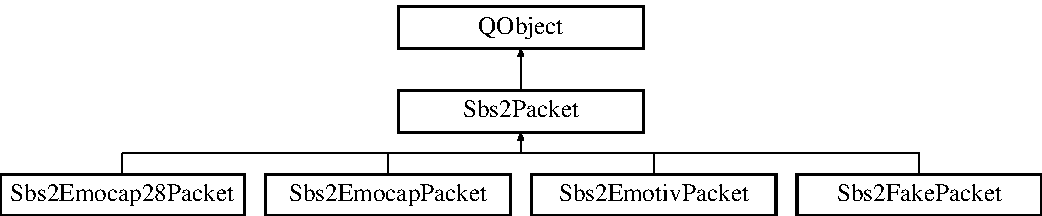
\includegraphics[height=2.896552cm]{classSbs2Packet}
\end{center}
\end{figure}
\subsection*{Public Member Functions}
\begin{DoxyCompactItemize}
\item 
\hyperlink{classSbs2Packet_a092be5f534662370b7d20f78abee1adb}{Sbs2\-Packet} (Q\-Object $\ast$parent=0)
\begin{DoxyCompactList}\small\item\em Constructor Constructs empty packet. \end{DoxyCompactList}\item 
virtual void \hyperlink{classSbs2Packet_a8b80c76000ceead51e9278c833bb56ae}{update} (char $\ast$data)
\begin{DoxyCompactList}\small\item\em Method for updating data in the packet. To avoid continuous creation and destruction of objects, certain number of empty packets is constructed in initialization and then updated with wrap-\/around. Packets should see the raw data delieverd by \hyperlink{classSbs2DataReader}{Sbs2\-Data\-Reader} and form themselves. \end{DoxyCompactList}\end{DoxyCompactItemize}
\subsection*{Public Attributes}
\begin{DoxyCompactItemize}
\item 
int \hyperlink{classSbs2Packet_af326a6f42a0486d08dbd17606ea7efaa}{counter}
\item 
int \hyperlink{classSbs2Packet_a2a086b322eba8c8d7754316eebefb0d1}{gyro\-X}
\item 
int \hyperlink{classSbs2Packet_aff1fc6891bbc36618c7e6434fe41e9bb}{gyro\-Y}
\item 
int \hyperlink{classSbs2Packet_a855c38df71a3630c692712afc686f29a}{cq}
\item 
int \hyperlink{classSbs2Packet_aa2dc8c43674d8dde85cb5cddfb86d46d}{cq\-Index}
\item 
Q\-String \hyperlink{classSbs2Packet_a548d8e8a0a00c3885143fe66fb6bd2b9}{cq\-Name}
\item 
Q\-Map$<$ Q\-String, double $>$ \hyperlink{classSbs2Packet_a48d32912f9a418d6073867760c74c345}{values}
\item 
Q\-Map$<$ Q\-String, double $>$ \hyperlink{classSbs2Packet_a910213b186d242ecc610a5d314d6115f}{filtered\-Values}
\item 
int \hyperlink{classSbs2Packet_a32fadc0b6ffe84dcba03ee3a943e1828}{battery}
\item 
char $\ast$ \hyperlink{classSbs2Packet_a9f8b30bbf48424b92e9ec0491dd04843}{raw\-Data}
\end{DoxyCompactItemize}


\subsection{Constructor \& Destructor Documentation}
\hypertarget{classSbs2Packet_a092be5f534662370b7d20f78abee1adb}{\index{Sbs2\-Packet@{Sbs2\-Packet}!Sbs2\-Packet@{Sbs2\-Packet}}
\index{Sbs2\-Packet@{Sbs2\-Packet}!Sbs2Packet@{Sbs2\-Packet}}
\subsubsection[{Sbs2\-Packet}]{\setlength{\rightskip}{0pt plus 5cm}Sbs2\-Packet\-::\-Sbs2\-Packet (
\begin{DoxyParamCaption}
\item[{Q\-Object $\ast$}]{parent = {\ttfamily 0}}
\end{DoxyParamCaption}
)\hspace{0.3cm}{\ttfamily [explicit]}}}\label{classSbs2Packet_a092be5f534662370b7d20f78abee1adb}


Constructor Constructs empty packet. 


\begin{DoxyParams}{Parameters}
{\em parent} & Pointer to teh parent Q\-Object object. \\
\hline
\end{DoxyParams}


\subsection{Member Function Documentation}
\hypertarget{classSbs2Packet_a8b80c76000ceead51e9278c833bb56ae}{\index{Sbs2\-Packet@{Sbs2\-Packet}!update@{update}}
\index{update@{update}!Sbs2Packet@{Sbs2\-Packet}}
\subsubsection[{update}]{\setlength{\rightskip}{0pt plus 5cm}void Sbs2\-Packet\-::update (
\begin{DoxyParamCaption}
\item[{char $\ast$}]{data}
\end{DoxyParamCaption}
)\hspace{0.3cm}{\ttfamily [virtual]}}}\label{classSbs2Packet_a8b80c76000ceead51e9278c833bb56ae}


Method for updating data in the packet. To avoid continuous creation and destruction of objects, certain number of empty packets is constructed in initialization and then updated with wrap-\/around. Packets should see the raw data delieverd by \hyperlink{classSbs2DataReader}{Sbs2\-Data\-Reader} and form themselves. 


\begin{DoxyParams}{Parameters}
{\em data} & Pointer to raw data. \\
\hline
\end{DoxyParams}


Reimplemented in \hyperlink{classSbs2EmocapPacket_a68263221ddb233ea7d8da392203a523e}{Sbs2\-Emocap\-Packet}, \hyperlink{classSbs2Emocap28Packet_a5fe0695a677da249df1226c310926716}{Sbs2\-Emocap28\-Packet}, and \hyperlink{classSbs2EmotivPacket_aaf8b25e8f747bbb80d7dcc5853d6e814}{Sbs2\-Emotiv\-Packet}.



\subsection{Member Data Documentation}
\hypertarget{classSbs2Packet_a32fadc0b6ffe84dcba03ee3a943e1828}{\index{Sbs2\-Packet@{Sbs2\-Packet}!battery@{battery}}
\index{battery@{battery}!Sbs2Packet@{Sbs2\-Packet}}
\subsubsection[{battery}]{\setlength{\rightskip}{0pt plus 5cm}int Sbs2\-Packet\-::battery}}\label{classSbs2Packet_a32fadc0b6ffe84dcba03ee3a943e1828}
\hypertarget{classSbs2Packet_af326a6f42a0486d08dbd17606ea7efaa}{\index{Sbs2\-Packet@{Sbs2\-Packet}!counter@{counter}}
\index{counter@{counter}!Sbs2Packet@{Sbs2\-Packet}}
\subsubsection[{counter}]{\setlength{\rightskip}{0pt plus 5cm}int Sbs2\-Packet\-::counter}}\label{classSbs2Packet_af326a6f42a0486d08dbd17606ea7efaa}
\hypertarget{classSbs2Packet_a855c38df71a3630c692712afc686f29a}{\index{Sbs2\-Packet@{Sbs2\-Packet}!cq@{cq}}
\index{cq@{cq}!Sbs2Packet@{Sbs2\-Packet}}
\subsubsection[{cq}]{\setlength{\rightskip}{0pt plus 5cm}int Sbs2\-Packet\-::cq}}\label{classSbs2Packet_a855c38df71a3630c692712afc686f29a}
\hypertarget{classSbs2Packet_aa2dc8c43674d8dde85cb5cddfb86d46d}{\index{Sbs2\-Packet@{Sbs2\-Packet}!cq\-Index@{cq\-Index}}
\index{cq\-Index@{cq\-Index}!Sbs2Packet@{Sbs2\-Packet}}
\subsubsection[{cq\-Index}]{\setlength{\rightskip}{0pt plus 5cm}int Sbs2\-Packet\-::cq\-Index}}\label{classSbs2Packet_aa2dc8c43674d8dde85cb5cddfb86d46d}
\hypertarget{classSbs2Packet_a548d8e8a0a00c3885143fe66fb6bd2b9}{\index{Sbs2\-Packet@{Sbs2\-Packet}!cq\-Name@{cq\-Name}}
\index{cq\-Name@{cq\-Name}!Sbs2Packet@{Sbs2\-Packet}}
\subsubsection[{cq\-Name}]{\setlength{\rightskip}{0pt plus 5cm}Q\-String Sbs2\-Packet\-::cq\-Name}}\label{classSbs2Packet_a548d8e8a0a00c3885143fe66fb6bd2b9}
\hypertarget{classSbs2Packet_a910213b186d242ecc610a5d314d6115f}{\index{Sbs2\-Packet@{Sbs2\-Packet}!filtered\-Values@{filtered\-Values}}
\index{filtered\-Values@{filtered\-Values}!Sbs2Packet@{Sbs2\-Packet}}
\subsubsection[{filtered\-Values}]{\setlength{\rightskip}{0pt plus 5cm}Q\-Map$<$Q\-String, double$>$ Sbs2\-Packet\-::filtered\-Values}}\label{classSbs2Packet_a910213b186d242ecc610a5d314d6115f}
\hypertarget{classSbs2Packet_a2a086b322eba8c8d7754316eebefb0d1}{\index{Sbs2\-Packet@{Sbs2\-Packet}!gyro\-X@{gyro\-X}}
\index{gyro\-X@{gyro\-X}!Sbs2Packet@{Sbs2\-Packet}}
\subsubsection[{gyro\-X}]{\setlength{\rightskip}{0pt plus 5cm}int Sbs2\-Packet\-::gyro\-X}}\label{classSbs2Packet_a2a086b322eba8c8d7754316eebefb0d1}
\hypertarget{classSbs2Packet_aff1fc6891bbc36618c7e6434fe41e9bb}{\index{Sbs2\-Packet@{Sbs2\-Packet}!gyro\-Y@{gyro\-Y}}
\index{gyro\-Y@{gyro\-Y}!Sbs2Packet@{Sbs2\-Packet}}
\subsubsection[{gyro\-Y}]{\setlength{\rightskip}{0pt plus 5cm}int Sbs2\-Packet\-::gyro\-Y}}\label{classSbs2Packet_aff1fc6891bbc36618c7e6434fe41e9bb}
\hypertarget{classSbs2Packet_a9f8b30bbf48424b92e9ec0491dd04843}{\index{Sbs2\-Packet@{Sbs2\-Packet}!raw\-Data@{raw\-Data}}
\index{raw\-Data@{raw\-Data}!Sbs2Packet@{Sbs2\-Packet}}
\subsubsection[{raw\-Data}]{\setlength{\rightskip}{0pt plus 5cm}char$\ast$ Sbs2\-Packet\-::raw\-Data}}\label{classSbs2Packet_a9f8b30bbf48424b92e9ec0491dd04843}
\hypertarget{classSbs2Packet_a48d32912f9a418d6073867760c74c345}{\index{Sbs2\-Packet@{Sbs2\-Packet}!values@{values}}
\index{values@{values}!Sbs2Packet@{Sbs2\-Packet}}
\subsubsection[{values}]{\setlength{\rightskip}{0pt plus 5cm}Q\-Map$<$Q\-String, double$>$ Sbs2\-Packet\-::values}}\label{classSbs2Packet_a48d32912f9a418d6073867760c74c345}


The documentation for this class was generated from the following files\-:\begin{DoxyCompactItemize}
\item 
/media/philipjhj/\-Data/\-One\-Drive/\-Studie/\-Studenterprogrammør/\-S\-B\-S3/smartphonebrainscanner2-\/core/src/hardware/\hyperlink{sbs2packet_8h}{sbs2packet.\-h}\item 
/media/philipjhj/\-Data/\-One\-Drive/\-Studie/\-Studenterprogrammør/\-S\-B\-S3/smartphonebrainscanner2-\/core/src/hardware/\hyperlink{sbs2packet_8cpp}{sbs2packet.\-cpp}\end{DoxyCompactItemize}

\hypertarget{classSbs2Region}{\section{Sbs2\-Region Class Reference}
\label{classSbs2Region}\index{Sbs2\-Region@{Sbs2\-Region}}
}


{\ttfamily \#include $<$sbs2region.\-h$>$}

Inheritance diagram for Sbs2\-Region\-:\begin{figure}[H]
\begin{center}
\leavevmode
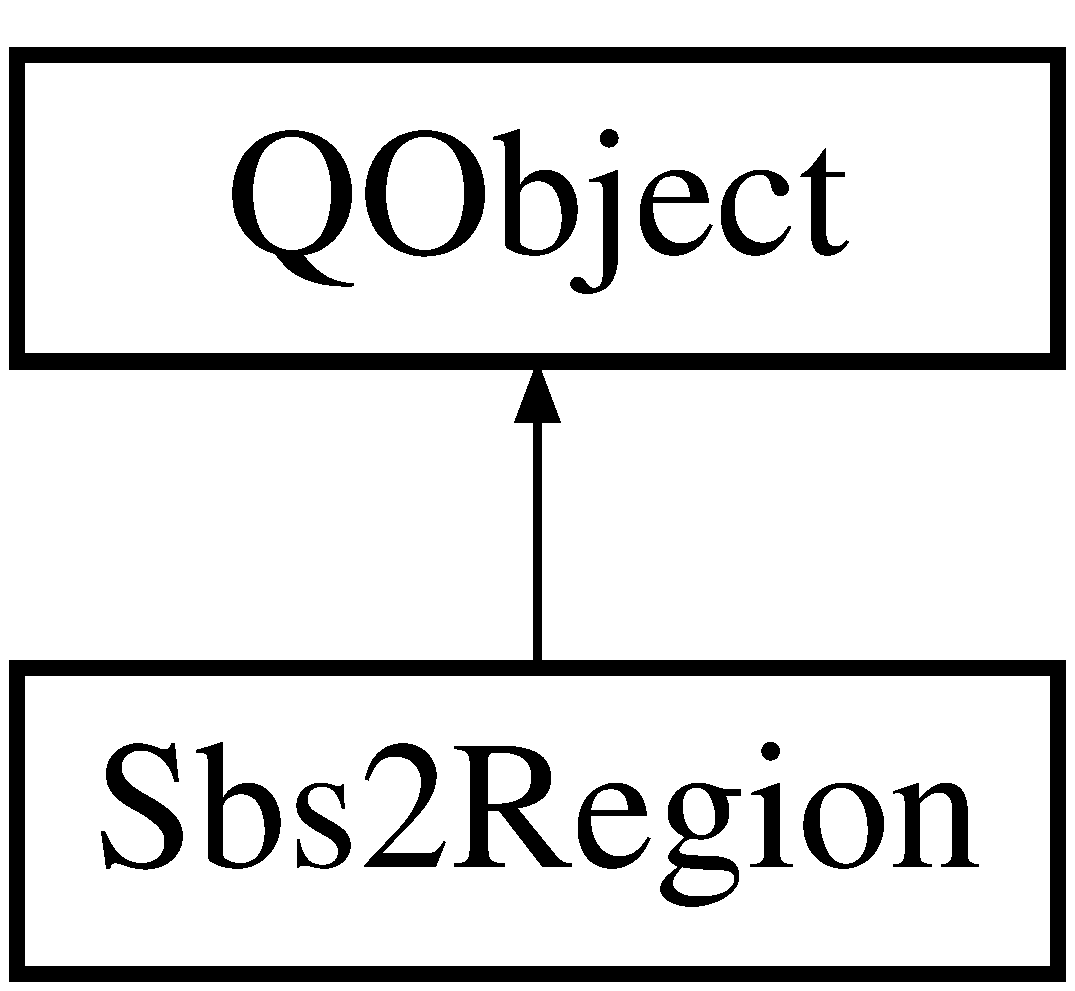
\includegraphics[height=2.000000cm]{classSbs2Region}
\end{center}
\end{figure}
\subsection*{Public Slots}
\begin{DoxyCompactItemize}
\item 
void \hyperlink{classSbs2Region_a2df365b69377caf571e693ee3f9d6c36}{clear\-Vertices\-To\-Extract} ()
\item 
void \hyperlink{classSbs2Region_a3767a2e0a62a59c399bd1b7a34d6b441}{add\-Region} (Q\-String region)
\item 
void \hyperlink{classSbs2Region_a41c5fc2f9ec94546bab50f026babb2ca}{add\-Regions\-Intersection} (Q\-String region1, Q\-String region2)
\end{DoxyCompactItemize}
\subsection*{Public Member Functions}
\begin{DoxyCompactItemize}
\item 
\hyperlink{classSbs2Region_a35c6902e7679c89dc21f73d38a43c17c}{Sbs2\-Region} (Q\-Object $\ast$parent=0)
\item 
Q\-Vector$<$ int $>$ $\ast$ \hyperlink{classSbs2Region_a0531f672554084e4e395fe505ccc9c76}{get\-Vertices\-To\-Extract} ()
\item 
Q\-Vector$<$ Q\-Vector$<$ int $>$ $>$ $\ast$ \hyperlink{classSbs2Region_a0afbdc01b6c101390ca36f7d7cd60833}{get\-Regions\-To\-Extract} ()
\end{DoxyCompactItemize}


\subsection{Detailed Description}
Smartphone Brain Scanner 2 License Agreement (M\-I\-T License)

Copyright (c) 2012 Arkadiusz Stopczynski, Jakob Eg Larsen, Carsten Stahlhut, Michael Kai Petersen, Lars Kai Hansen. Technical University of Denmark, \hyperlink{namespaceDTU}{D\-T\-U} Informatics, Cognitive Systems Section. \href{http://code.google.com/p/smartphonebrainscanner2}{\tt http\-://code.\-google.\-com/p/smartphonebrainscanner2}

Permission is hereby granted, free of charge, to any person obtaining a copy of this software and associated documentation files (the \char`\"{}\-Software\char`\"{}), to deal in the Software without restriction, including without limitation the rights to use, copy, modify, merge, publish, distribute, sublicense, and/or sell copies of the Software, and to permit persons to whom the Software is furnished to do so, subject to the following conditions\-:

The above copyright notice and this permission notice shall be included in all copies or substantial portions of the Software.

T\-H\-E S\-O\-F\-T\-W\-A\-R\-E I\-S P\-R\-O\-V\-I\-D\-E\-D \char`\"{}\-A\-S I\-S\char`\"{}, W\-I\-T\-H\-O\-U\-T W\-A\-R\-R\-A\-N\-T\-Y O\-F A\-N\-Y K\-I\-N\-D, E\-X\-P\-R\-E\-S\-S O\-R I\-M\-P\-L\-I\-E\-D, I\-N\-C\-L\-U\-D\-I\-N\-G B\-U\-T N\-O\-T L\-I\-M\-I\-T\-E\-D T\-O T\-H\-E W\-A\-R\-R\-A\-N\-T\-I\-E\-S O\-F M\-E\-R\-C\-H\-A\-N\-T\-A\-B\-I\-L\-I\-T\-Y, F\-I\-T\-N\-E\-S\-S F\-O\-R A P\-A\-R\-T\-I\-C\-U\-L\-A\-R P\-U\-R\-P\-O\-S\-E A\-N\-D N\-O\-N\-I\-N\-F\-R\-I\-N\-G\-E\-M\-E\-N\-T. I\-N N\-O E\-V\-E\-N\-T S\-H\-A\-L\-L T\-H\-E A\-U\-T\-H\-O\-R\-S O\-R C\-O\-P\-Y\-R\-I\-G\-H\-T H\-O\-L\-D\-E\-R\-S B\-E L\-I\-A\-B\-L\-E F\-O\-R A\-N\-Y C\-L\-A\-I\-M, D\-A\-M\-A\-G\-E\-S O\-R O\-T\-H\-E\-R L\-I\-A\-B\-I\-L\-I\-T\-Y, W\-H\-E\-T\-H\-E\-R I\-N A\-N A\-C\-T\-I\-O\-N O\-F C\-O\-N\-T\-R\-A\-C\-T, T\-O\-R\-T O\-R O\-T\-H\-E\-R\-W\-I\-S\-E, A\-R\-I\-S\-I\-N\-G F\-R\-O\-M, O\-U\-T O\-F O\-R I\-N C\-O\-N\-N\-E\-C\-T\-I\-O\-N W\-I\-T\-H T\-H\-E S\-O\-F\-T\-W\-A\-R\-E O\-R T\-H\-E U\-S\-E O\-R O\-T\-H\-E\-R D\-E\-A\-L\-I\-N\-G\-S I\-N T\-H\-E S\-O\-F\-T\-W\-A\-R\-E. 

\subsection{Constructor \& Destructor Documentation}
\hypertarget{classSbs2Region_a35c6902e7679c89dc21f73d38a43c17c}{\index{Sbs2\-Region@{Sbs2\-Region}!Sbs2\-Region@{Sbs2\-Region}}
\index{Sbs2\-Region@{Sbs2\-Region}!Sbs2Region@{Sbs2\-Region}}
\subsubsection[{Sbs2\-Region}]{\setlength{\rightskip}{0pt plus 5cm}Sbs2\-Region\-::\-Sbs2\-Region (
\begin{DoxyParamCaption}
\item[{Q\-Object $\ast$}]{parent = {\ttfamily 0}}
\end{DoxyParamCaption}
)\hspace{0.3cm}{\ttfamily [explicit]}}}\label{classSbs2Region_a35c6902e7679c89dc21f73d38a43c17c}


\subsection{Member Function Documentation}
\hypertarget{classSbs2Region_a3767a2e0a62a59c399bd1b7a34d6b441}{\index{Sbs2\-Region@{Sbs2\-Region}!add\-Region@{add\-Region}}
\index{add\-Region@{add\-Region}!Sbs2Region@{Sbs2\-Region}}
\subsubsection[{add\-Region}]{\setlength{\rightskip}{0pt plus 5cm}void Sbs2\-Region\-::add\-Region (
\begin{DoxyParamCaption}
\item[{Q\-String}]{region}
\end{DoxyParamCaption}
)\hspace{0.3cm}{\ttfamily [slot]}}}\label{classSbs2Region_a3767a2e0a62a59c399bd1b7a34d6b441}
\hypertarget{classSbs2Region_a41c5fc2f9ec94546bab50f026babb2ca}{\index{Sbs2\-Region@{Sbs2\-Region}!add\-Regions\-Intersection@{add\-Regions\-Intersection}}
\index{add\-Regions\-Intersection@{add\-Regions\-Intersection}!Sbs2Region@{Sbs2\-Region}}
\subsubsection[{add\-Regions\-Intersection}]{\setlength{\rightskip}{0pt plus 5cm}void Sbs2\-Region\-::add\-Regions\-Intersection (
\begin{DoxyParamCaption}
\item[{Q\-String}]{region1, }
\item[{Q\-String}]{region2}
\end{DoxyParamCaption}
)\hspace{0.3cm}{\ttfamily [slot]}}}\label{classSbs2Region_a41c5fc2f9ec94546bab50f026babb2ca}
\hypertarget{classSbs2Region_a2df365b69377caf571e693ee3f9d6c36}{\index{Sbs2\-Region@{Sbs2\-Region}!clear\-Vertices\-To\-Extract@{clear\-Vertices\-To\-Extract}}
\index{clear\-Vertices\-To\-Extract@{clear\-Vertices\-To\-Extract}!Sbs2Region@{Sbs2\-Region}}
\subsubsection[{clear\-Vertices\-To\-Extract}]{\setlength{\rightskip}{0pt plus 5cm}void Sbs2\-Region\-::clear\-Vertices\-To\-Extract (
\begin{DoxyParamCaption}
{}
\end{DoxyParamCaption}
)\hspace{0.3cm}{\ttfamily [slot]}}}\label{classSbs2Region_a2df365b69377caf571e693ee3f9d6c36}
\hypertarget{classSbs2Region_a0afbdc01b6c101390ca36f7d7cd60833}{\index{Sbs2\-Region@{Sbs2\-Region}!get\-Regions\-To\-Extract@{get\-Regions\-To\-Extract}}
\index{get\-Regions\-To\-Extract@{get\-Regions\-To\-Extract}!Sbs2Region@{Sbs2\-Region}}
\subsubsection[{get\-Regions\-To\-Extract}]{\setlength{\rightskip}{0pt plus 5cm}Q\-Vector$<$ Q\-Vector$<$ int $>$ $>$ $\ast$ Sbs2\-Region\-::get\-Regions\-To\-Extract (
\begin{DoxyParamCaption}
{}
\end{DoxyParamCaption}
)}}\label{classSbs2Region_a0afbdc01b6c101390ca36f7d7cd60833}
\hypertarget{classSbs2Region_a0531f672554084e4e395fe505ccc9c76}{\index{Sbs2\-Region@{Sbs2\-Region}!get\-Vertices\-To\-Extract@{get\-Vertices\-To\-Extract}}
\index{get\-Vertices\-To\-Extract@{get\-Vertices\-To\-Extract}!Sbs2Region@{Sbs2\-Region}}
\subsubsection[{get\-Vertices\-To\-Extract}]{\setlength{\rightskip}{0pt plus 5cm}Q\-Vector$<$ int $>$ $\ast$ Sbs2\-Region\-::get\-Vertices\-To\-Extract (
\begin{DoxyParamCaption}
{}
\end{DoxyParamCaption}
)}}\label{classSbs2Region_a0531f672554084e4e395fe505ccc9c76}


The documentation for this class was generated from the following files\-:\begin{DoxyCompactItemize}
\item 
/media/philipjhj/\-Data/\-One\-Drive/\-Studie/\-Studenterprogrammør/\-S\-B\-S3/smartphonebrainscanner2-\/core/src/\hyperlink{sbs2region_8h}{sbs2region.\-h}\item 
/media/philipjhj/\-Data/\-One\-Drive/\-Studie/\-Studenterprogrammør/\-S\-B\-S3/smartphonebrainscanner2-\/core/src/\hyperlink{sbs2region_8cpp}{sbs2region.\-cpp}\end{DoxyCompactItemize}

\hypertarget{classSbs2SourceReconstrucionLoreta}{\section{Sbs2\-Source\-Reconstrucion\-Loreta Class Reference}
\label{classSbs2SourceReconstrucionLoreta}\index{Sbs2\-Source\-Reconstrucion\-Loreta@{Sbs2\-Source\-Reconstrucion\-Loreta}}
}


{\ttfamily \#include $<$sbs2sourcereconstruction\-\_\-loreta.\-h$>$}

Inheritance diagram for Sbs2\-Source\-Reconstrucion\-Loreta\-:\begin{figure}[H]
\begin{center}
\leavevmode
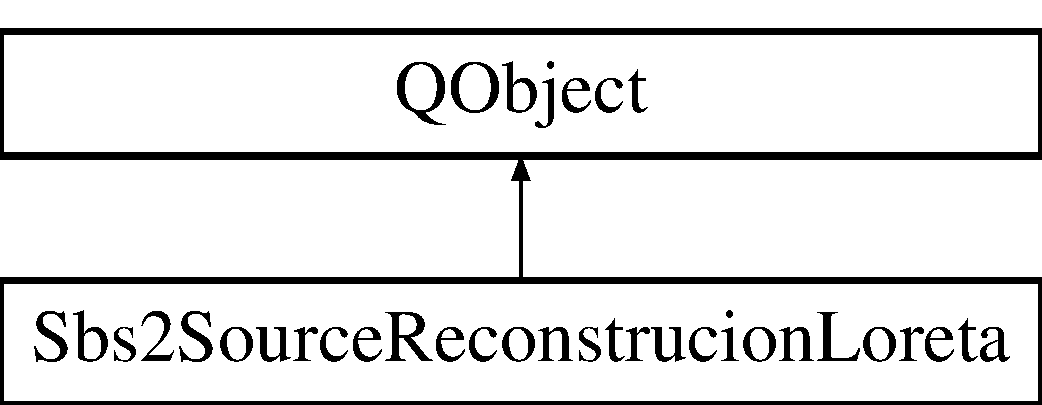
\includegraphics[height=2.000000cm]{classSbs2SourceReconstrucionLoreta}
\end{center}
\end{figure}
\subsection*{Public Types}
\begin{DoxyCompactItemize}
\item 
enum \hyperlink{classSbs2SourceReconstrucionLoreta_aebf0de7b32b377d64f23f1bf71c119f7}{Sum\-Type} \{ \hyperlink{classSbs2SourceReconstrucionLoreta_aebf0de7b32b377d64f23f1bf71c119f7afc730e604c373aa6245980e92fcc14af}{M\-E\-A\-N}, 
\hyperlink{classSbs2SourceReconstrucionLoreta_aebf0de7b32b377d64f23f1bf71c119f7ad1e58d65e4f8e7977e07100eeeb056c7}{P\-O\-W\-E\-R}
 \}
\end{DoxyCompactItemize}
\subsection*{Public Slots}
\begin{DoxyCompactItemize}
\item 
void \hyperlink{classSbs2SourceReconstrucionLoreta_a1d8f39e7aaceeffede70e9c16fe2847b}{set\-Sum\-Type} (\hyperlink{classSbs2SourceReconstrucionLoreta_aebf0de7b32b377d64f23f1bf71c119f7}{Sum\-Type} sum\-Type\-\_\-)
\begin{DoxyCompactList}\small\item\em Sbs2\-Source\-Reconstrucion\-::set\-Sum\-Type. \end{DoxyCompactList}\item 
void \hyperlink{classSbs2SourceReconstrucionLoreta_a12b14c29ebe6c3a2a04f216206a572d7}{set\-Mean\-Extraction} (int enabled)
\item 
void \hyperlink{classSbs2SourceReconstrucionLoreta_a8b46d92b0bdb35d38224c06ab3ab9f70}{set\-A\-Scaling} (int scaling)
\item 
void \hyperlink{classSbs2SourceReconstrucionLoreta_a1dcd35bbd82f8157c00778e9f2e51610}{set\-Vertices\-To\-Extract} (Q\-Vector$<$ int $>$ $\ast$vertices\-To\-Extract\-\_\-)
\item 
void \hyperlink{classSbs2SourceReconstrucionLoreta_ae65de60277bf2934800b2eacacc37a68}{do\-Rec} (\hyperlink{classDTU_1_1DtuArray2D}{D\-T\-U\-::\-Dtu\-Array2\-D}$<$ double $>$ $\ast$input\-\_\-, \hyperlink{classDTU_1_1DtuArray2D}{D\-T\-U\-::\-Dtu\-Array2\-D}$<$ double $>$ $\ast$output\-\_\-, int $\ast$source\-Reconstruction\-Ready)
\item 
void \hyperlink{classSbs2SourceReconstrucionLoreta_a16f7bb0a19cccb1e8520d315135506db}{do\-Rec\-Pow} (\hyperlink{classDTU_1_1DtuArray2D}{D\-T\-U\-::\-Dtu\-Array2\-D}$<$ double $>$ $\ast$input\-\_\-, \hyperlink{classDTU_1_1DtuArray2D}{D\-T\-U\-::\-Dtu\-Array2\-D}$<$ double $>$ $\ast$output\-\_\-, int $\ast$source\-Reconstrution\-Ready)
\end{DoxyCompactItemize}
\subsection*{Public Member Functions}
\begin{DoxyCompactItemize}
\item 
\hyperlink{classSbs2SourceReconstrucionLoreta_ac7dfbacf96035d958a698dfd23108ba9}{Sbs2\-Source\-Reconstrucion\-Loreta} (int channels\-\_\-, int samples\-\_\-, int samples\-Delta\-\_\-, int vertices\-\_\-, Q\-String hardware\-\_\-, Q\-Object $\ast$parent\-\_\-, int model\-Update\-Length\-\_\-=8, int model\-Update\-Delta\-\_\-=24)
\end{DoxyCompactItemize}
\subsection*{Public Attributes}
\begin{DoxyCompactItemize}
\item 
int \hyperlink{classSbs2SourceReconstrucionLoreta_a761881bfe0455685f6434f66142c5326}{temp\-Model\-Updated\-Ready}
\end{DoxyCompactItemize}


\subsection{Member Enumeration Documentation}
\hypertarget{classSbs2SourceReconstrucionLoreta_aebf0de7b32b377d64f23f1bf71c119f7}{\index{Sbs2\-Source\-Reconstrucion\-Loreta@{Sbs2\-Source\-Reconstrucion\-Loreta}!Sum\-Type@{Sum\-Type}}
\index{Sum\-Type@{Sum\-Type}!Sbs2SourceReconstrucionLoreta@{Sbs2\-Source\-Reconstrucion\-Loreta}}
\subsubsection[{Sum\-Type}]{\setlength{\rightskip}{0pt plus 5cm}enum {\bf Sbs2\-Source\-Reconstrucion\-Loreta\-::\-Sum\-Type}}}\label{classSbs2SourceReconstrucionLoreta_aebf0de7b32b377d64f23f1bf71c119f7}
\begin{Desc}
\item[Enumerator]\par
\begin{description}
\index{M\-E\-A\-N@{M\-E\-A\-N}!Sbs2\-Source\-Reconstrucion\-Loreta@{Sbs2\-Source\-Reconstrucion\-Loreta}}\index{Sbs2\-Source\-Reconstrucion\-Loreta@{Sbs2\-Source\-Reconstrucion\-Loreta}!M\-E\-A\-N@{M\-E\-A\-N}}\item[{\em 
\hypertarget{classSbs2SourceReconstrucionLoreta_aebf0de7b32b377d64f23f1bf71c119f7afc730e604c373aa6245980e92fcc14af}{M\-E\-A\-N}\label{classSbs2SourceReconstrucionLoreta_aebf0de7b32b377d64f23f1bf71c119f7afc730e604c373aa6245980e92fcc14af}
}]\index{P\-O\-W\-E\-R@{P\-O\-W\-E\-R}!Sbs2\-Source\-Reconstrucion\-Loreta@{Sbs2\-Source\-Reconstrucion\-Loreta}}\index{Sbs2\-Source\-Reconstrucion\-Loreta@{Sbs2\-Source\-Reconstrucion\-Loreta}!P\-O\-W\-E\-R@{P\-O\-W\-E\-R}}\item[{\em 
\hypertarget{classSbs2SourceReconstrucionLoreta_aebf0de7b32b377d64f23f1bf71c119f7ad1e58d65e4f8e7977e07100eeeb056c7}{P\-O\-W\-E\-R}\label{classSbs2SourceReconstrucionLoreta_aebf0de7b32b377d64f23f1bf71c119f7ad1e58d65e4f8e7977e07100eeeb056c7}
}]\end{description}
\end{Desc}


\subsection{Constructor \& Destructor Documentation}
\hypertarget{classSbs2SourceReconstrucionLoreta_ac7dfbacf96035d958a698dfd23108ba9}{\index{Sbs2\-Source\-Reconstrucion\-Loreta@{Sbs2\-Source\-Reconstrucion\-Loreta}!Sbs2\-Source\-Reconstrucion\-Loreta@{Sbs2\-Source\-Reconstrucion\-Loreta}}
\index{Sbs2\-Source\-Reconstrucion\-Loreta@{Sbs2\-Source\-Reconstrucion\-Loreta}!Sbs2SourceReconstrucionLoreta@{Sbs2\-Source\-Reconstrucion\-Loreta}}
\subsubsection[{Sbs2\-Source\-Reconstrucion\-Loreta}]{\setlength{\rightskip}{0pt plus 5cm}Sbs2\-Source\-Reconstrucion\-Loreta\-::\-Sbs2\-Source\-Reconstrucion\-Loreta (
\begin{DoxyParamCaption}
\item[{int}]{channels\-\_\-, }
\item[{int}]{samples\-\_\-, }
\item[{int}]{samples\-Delta\-\_\-, }
\item[{int}]{vertices\-\_\-, }
\item[{Q\-String}]{hardware\-\_\-, }
\item[{Q\-Object $\ast$}]{parent\-\_\-, }
\item[{int}]{model\-Update\-Length\-\_\- = {\ttfamily 8}, }
\item[{int}]{model\-Update\-Delta\-\_\- = {\ttfamily 24}}
\end{DoxyParamCaption}
)\hspace{0.3cm}{\ttfamily [explicit]}}}\label{classSbs2SourceReconstrucionLoreta_ac7dfbacf96035d958a698dfd23108ba9}


\subsection{Member Function Documentation}
\hypertarget{classSbs2SourceReconstrucionLoreta_ae65de60277bf2934800b2eacacc37a68}{\index{Sbs2\-Source\-Reconstrucion\-Loreta@{Sbs2\-Source\-Reconstrucion\-Loreta}!do\-Rec@{do\-Rec}}
\index{do\-Rec@{do\-Rec}!Sbs2SourceReconstrucionLoreta@{Sbs2\-Source\-Reconstrucion\-Loreta}}
\subsubsection[{do\-Rec}]{\setlength{\rightskip}{0pt plus 5cm}void Sbs2\-Source\-Reconstrucion\-Loreta\-::do\-Rec (
\begin{DoxyParamCaption}
\item[{{\bf D\-T\-U\-::\-Dtu\-Array2\-D}$<$ double $>$ $\ast$}]{input\-\_\-, }
\item[{{\bf D\-T\-U\-::\-Dtu\-Array2\-D}$<$ double $>$ $\ast$}]{output\-\_\-, }
\item[{int $\ast$}]{source\-Reconstruction\-Ready}
\end{DoxyParamCaption}
)\hspace{0.3cm}{\ttfamily [slot]}}}\label{classSbs2SourceReconstrucionLoreta_ae65de60277bf2934800b2eacacc37a68}
\hypertarget{classSbs2SourceReconstrucionLoreta_a16f7bb0a19cccb1e8520d315135506db}{\index{Sbs2\-Source\-Reconstrucion\-Loreta@{Sbs2\-Source\-Reconstrucion\-Loreta}!do\-Rec\-Pow@{do\-Rec\-Pow}}
\index{do\-Rec\-Pow@{do\-Rec\-Pow}!Sbs2SourceReconstrucionLoreta@{Sbs2\-Source\-Reconstrucion\-Loreta}}
\subsubsection[{do\-Rec\-Pow}]{\setlength{\rightskip}{0pt plus 5cm}void Sbs2\-Source\-Reconstrucion\-Loreta\-::do\-Rec\-Pow (
\begin{DoxyParamCaption}
\item[{{\bf D\-T\-U\-::\-Dtu\-Array2\-D}$<$ double $>$ $\ast$}]{input\-\_\-, }
\item[{{\bf D\-T\-U\-::\-Dtu\-Array2\-D}$<$ double $>$ $\ast$}]{output\-\_\-, }
\item[{int $\ast$}]{source\-Reconstrution\-Ready}
\end{DoxyParamCaption}
)\hspace{0.3cm}{\ttfamily [slot]}}}\label{classSbs2SourceReconstrucionLoreta_a16f7bb0a19cccb1e8520d315135506db}
\hypertarget{classSbs2SourceReconstrucionLoreta_a8b46d92b0bdb35d38224c06ab3ab9f70}{\index{Sbs2\-Source\-Reconstrucion\-Loreta@{Sbs2\-Source\-Reconstrucion\-Loreta}!set\-A\-Scaling@{set\-A\-Scaling}}
\index{set\-A\-Scaling@{set\-A\-Scaling}!Sbs2SourceReconstrucionLoreta@{Sbs2\-Source\-Reconstrucion\-Loreta}}
\subsubsection[{set\-A\-Scaling}]{\setlength{\rightskip}{0pt plus 5cm}void Sbs2\-Source\-Reconstrucion\-Loreta\-::set\-A\-Scaling (
\begin{DoxyParamCaption}
\item[{int}]{scaling}
\end{DoxyParamCaption}
)\hspace{0.3cm}{\ttfamily [slot]}}}\label{classSbs2SourceReconstrucionLoreta_a8b46d92b0bdb35d38224c06ab3ab9f70}
\hypertarget{classSbs2SourceReconstrucionLoreta_a12b14c29ebe6c3a2a04f216206a572d7}{\index{Sbs2\-Source\-Reconstrucion\-Loreta@{Sbs2\-Source\-Reconstrucion\-Loreta}!set\-Mean\-Extraction@{set\-Mean\-Extraction}}
\index{set\-Mean\-Extraction@{set\-Mean\-Extraction}!Sbs2SourceReconstrucionLoreta@{Sbs2\-Source\-Reconstrucion\-Loreta}}
\subsubsection[{set\-Mean\-Extraction}]{\setlength{\rightskip}{0pt plus 5cm}void Sbs2\-Source\-Reconstrucion\-Loreta\-::set\-Mean\-Extraction (
\begin{DoxyParamCaption}
\item[{int}]{enabled}
\end{DoxyParamCaption}
)\hspace{0.3cm}{\ttfamily [slot]}}}\label{classSbs2SourceReconstrucionLoreta_a12b14c29ebe6c3a2a04f216206a572d7}
\hypertarget{classSbs2SourceReconstrucionLoreta_a1d8f39e7aaceeffede70e9c16fe2847b}{\index{Sbs2\-Source\-Reconstrucion\-Loreta@{Sbs2\-Source\-Reconstrucion\-Loreta}!set\-Sum\-Type@{set\-Sum\-Type}}
\index{set\-Sum\-Type@{set\-Sum\-Type}!Sbs2SourceReconstrucionLoreta@{Sbs2\-Source\-Reconstrucion\-Loreta}}
\subsubsection[{set\-Sum\-Type}]{\setlength{\rightskip}{0pt plus 5cm}void Sbs2\-Source\-Reconstrucion\-Loreta\-::set\-Sum\-Type (
\begin{DoxyParamCaption}
\item[{{\bf Sum\-Type}}]{sum\-Type\-\_\-}
\end{DoxyParamCaption}
)\hspace{0.3cm}{\ttfamily [slot]}}}\label{classSbs2SourceReconstrucionLoreta_a1d8f39e7aaceeffede70e9c16fe2847b}


Sbs2\-Source\-Reconstrucion\-::set\-Sum\-Type. 


\begin{DoxyParams}{Parameters}
{\em sum\-Type\-\_\-} & should be either 'M\-E\-A\-N' or 'S\-U\-M'\\
\hline
\end{DoxyParams}
Set the 'sum\-Type' variable \hypertarget{classSbs2SourceReconstrucionLoreta_a1dcd35bbd82f8157c00778e9f2e51610}{\index{Sbs2\-Source\-Reconstrucion\-Loreta@{Sbs2\-Source\-Reconstrucion\-Loreta}!set\-Vertices\-To\-Extract@{set\-Vertices\-To\-Extract}}
\index{set\-Vertices\-To\-Extract@{set\-Vertices\-To\-Extract}!Sbs2SourceReconstrucionLoreta@{Sbs2\-Source\-Reconstrucion\-Loreta}}
\subsubsection[{set\-Vertices\-To\-Extract}]{\setlength{\rightskip}{0pt plus 5cm}void Sbs2\-Source\-Reconstrucion\-Loreta\-::set\-Vertices\-To\-Extract (
\begin{DoxyParamCaption}
\item[{Q\-Vector$<$ int $>$ $\ast$}]{vertices\-To\-Extract\-\_\-}
\end{DoxyParamCaption}
)\hspace{0.3cm}{\ttfamily [slot]}}}\label{classSbs2SourceReconstrucionLoreta_a1dcd35bbd82f8157c00778e9f2e51610}


\subsection{Member Data Documentation}
\hypertarget{classSbs2SourceReconstrucionLoreta_a761881bfe0455685f6434f66142c5326}{\index{Sbs2\-Source\-Reconstrucion\-Loreta@{Sbs2\-Source\-Reconstrucion\-Loreta}!temp\-Model\-Updated\-Ready@{temp\-Model\-Updated\-Ready}}
\index{temp\-Model\-Updated\-Ready@{temp\-Model\-Updated\-Ready}!Sbs2SourceReconstrucionLoreta@{Sbs2\-Source\-Reconstrucion\-Loreta}}
\subsubsection[{temp\-Model\-Updated\-Ready}]{\setlength{\rightskip}{0pt plus 5cm}int Sbs2\-Source\-Reconstrucion\-Loreta\-::temp\-Model\-Updated\-Ready}}\label{classSbs2SourceReconstrucionLoreta_a761881bfe0455685f6434f66142c5326}


The documentation for this class was generated from the following files\-:\begin{DoxyCompactItemize}
\item 
/media/philipjhj/\-Data/\-One\-Drive/\-Studie/\-Studenterprogrammør/\-S\-B\-S3/smartphonebrainscanner2-\/core/src/source\-\_\-reconstruction/loreta/\hyperlink{sbs2sourcereconstruction__loreta_8h}{sbs2sourcereconstruction\-\_\-loreta.\-h}\item 
/media/philipjhj/\-Data/\-One\-Drive/\-Studie/\-Studenterprogrammør/\-S\-B\-S3/smartphonebrainscanner2-\/core/src/source\-\_\-reconstruction/loreta/\hyperlink{sbs2sourcereconstruction__loreta_8cpp}{sbs2sourcereconstruction\-\_\-loreta.\-cpp}\end{DoxyCompactItemize}

\hypertarget{classSbs2SourceReconstruction}{\section{Sbs2\-Source\-Reconstruction Class Reference}
\label{classSbs2SourceReconstruction}\index{Sbs2\-Source\-Reconstruction@{Sbs2\-Source\-Reconstruction}}
}


{\ttfamily \#include $<$sbs2sourcereconstruction.\-h$>$}

Inheritance diagram for Sbs2\-Source\-Reconstruction\-:\begin{figure}[H]
\begin{center}
\leavevmode
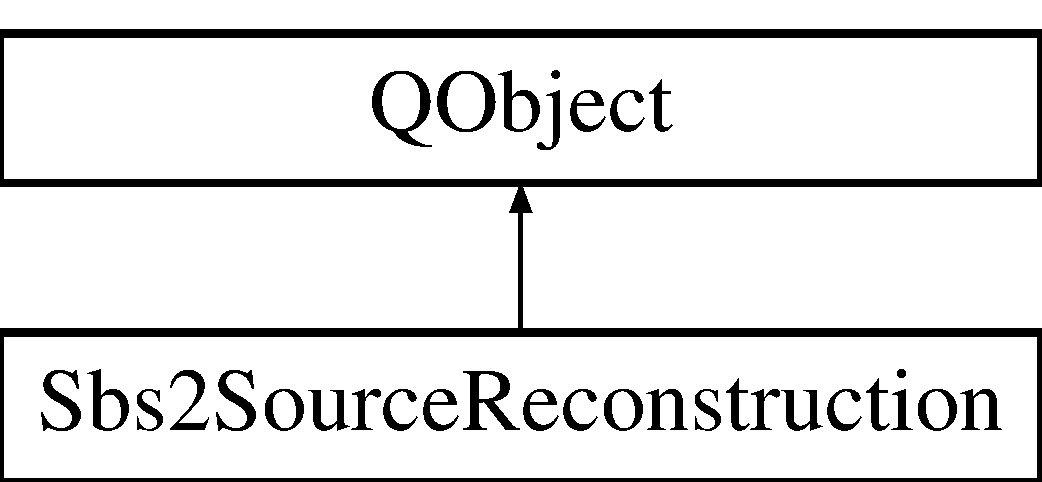
\includegraphics[height=2.000000cm]{classSbs2SourceReconstruction}
\end{center}
\end{figure}
\subsection*{Public Slots}
\begin{DoxyCompactItemize}
\item 
void \hyperlink{classSbs2SourceReconstruction_ae90a564e34f7973833de68151f8b03da}{turn\-On\-Loreta} (int source\-Reconstruction\-Samples, int source\-Reconstruction\-Delta, int source\-Reconstruction\-Model\-Update\-Length, int source\-Reconstruction\-Model\-Update\-Delta, Q\-String hardware, Q\-String source\-Reconstruction\-Method\-\_\-)
\item 
void \hyperlink{classSbs2SourceReconstruction_a63fffbdc6b14d6a3e1cb9f0a643f01b6}{turn\-On\-Sparse} (int source\-Reconstruction\-Samples, Q\-String hardware, Q\-Vector$<$ double $>$ lambdas, Q\-String source\-Reconstruction\-Method\-\_\-)
\item 
void \hyperlink{classSbs2SourceReconstruction_a6d812bfa61990f912e8d9a1b2346c030}{do\-Reconstruction} (\hyperlink{classDTU_1_1DtuArray2D}{D\-T\-U\-::\-Dtu\-Array2\-D}$<$ double $>$ $\ast$input\-\_\-, \hyperlink{classDTU_1_1DtuArray2D}{D\-T\-U\-::\-Dtu\-Array2\-D}$<$ double $>$ $\ast$output\-\_\-, int $\ast$source\-Reconstruction\-Ready)
\item 
void \hyperlink{classSbs2SourceReconstruction_af198fd9e278757ab86c3542c4e1eaca4}{do\-Reconstruction\-Spectrogram} (\hyperlink{classDTU_1_1DtuArray2D}{D\-T\-U\-::\-Dtu\-Array2\-D}$<$ double $>$ $\ast$input\-\_\-, \hyperlink{classDTU_1_1DtuArray2D}{D\-T\-U\-::\-Dtu\-Array2\-D}$<$ double $>$ $\ast$output\-\_\-, int $\ast$source\-Reconstruction\-Ready)
\item 
void \hyperlink{classSbs2SourceReconstruction_abf56fa85a9b63aa18592c2c4b84a2750}{stop\-Reconstruction} ()
\item 
void \hyperlink{classSbs2SourceReconstruction_a7456e6907f82ba461d9c4728f2bd8c40}{turn\-Off} ()
\end{DoxyCompactItemize}
\subsection*{Public Member Functions}
\begin{DoxyCompactItemize}
\item 
\hyperlink{classSbs2SourceReconstruction_a8fba578360e987641b11e9cc9bd5d9b8}{Sbs2\-Source\-Reconstruction} (Q\-Object $\ast$parent=0)
\end{DoxyCompactItemize}


\subsection{Constructor \& Destructor Documentation}
\hypertarget{classSbs2SourceReconstruction_a8fba578360e987641b11e9cc9bd5d9b8}{\index{Sbs2\-Source\-Reconstruction@{Sbs2\-Source\-Reconstruction}!Sbs2\-Source\-Reconstruction@{Sbs2\-Source\-Reconstruction}}
\index{Sbs2\-Source\-Reconstruction@{Sbs2\-Source\-Reconstruction}!Sbs2SourceReconstruction@{Sbs2\-Source\-Reconstruction}}
\subsubsection[{Sbs2\-Source\-Reconstruction}]{\setlength{\rightskip}{0pt plus 5cm}Sbs2\-Source\-Reconstruction\-::\-Sbs2\-Source\-Reconstruction (
\begin{DoxyParamCaption}
\item[{Q\-Object $\ast$}]{parent = {\ttfamily 0}}
\end{DoxyParamCaption}
)\hspace{0.3cm}{\ttfamily [explicit]}}}\label{classSbs2SourceReconstruction_a8fba578360e987641b11e9cc9bd5d9b8}


\subsection{Member Function Documentation}
\hypertarget{classSbs2SourceReconstruction_a6d812bfa61990f912e8d9a1b2346c030}{\index{Sbs2\-Source\-Reconstruction@{Sbs2\-Source\-Reconstruction}!do\-Reconstruction@{do\-Reconstruction}}
\index{do\-Reconstruction@{do\-Reconstruction}!Sbs2SourceReconstruction@{Sbs2\-Source\-Reconstruction}}
\subsubsection[{do\-Reconstruction}]{\setlength{\rightskip}{0pt plus 5cm}void Sbs2\-Source\-Reconstruction\-::do\-Reconstruction (
\begin{DoxyParamCaption}
\item[{{\bf D\-T\-U\-::\-Dtu\-Array2\-D}$<$ double $>$ $\ast$}]{input\-\_\-, }
\item[{{\bf D\-T\-U\-::\-Dtu\-Array2\-D}$<$ double $>$ $\ast$}]{output\-\_\-, }
\item[{int $\ast$}]{source\-Reconstruction\-Ready}
\end{DoxyParamCaption}
)\hspace{0.3cm}{\ttfamily [slot]}}}\label{classSbs2SourceReconstruction_a6d812bfa61990f912e8d9a1b2346c030}
\hypertarget{classSbs2SourceReconstruction_af198fd9e278757ab86c3542c4e1eaca4}{\index{Sbs2\-Source\-Reconstruction@{Sbs2\-Source\-Reconstruction}!do\-Reconstruction\-Spectrogram@{do\-Reconstruction\-Spectrogram}}
\index{do\-Reconstruction\-Spectrogram@{do\-Reconstruction\-Spectrogram}!Sbs2SourceReconstruction@{Sbs2\-Source\-Reconstruction}}
\subsubsection[{do\-Reconstruction\-Spectrogram}]{\setlength{\rightskip}{0pt plus 5cm}void Sbs2\-Source\-Reconstruction\-::do\-Reconstruction\-Spectrogram (
\begin{DoxyParamCaption}
\item[{{\bf D\-T\-U\-::\-Dtu\-Array2\-D}$<$ double $>$ $\ast$}]{input\-\_\-, }
\item[{{\bf D\-T\-U\-::\-Dtu\-Array2\-D}$<$ double $>$ $\ast$}]{output\-\_\-, }
\item[{int $\ast$}]{source\-Reconstruction\-Ready}
\end{DoxyParamCaption}
)\hspace{0.3cm}{\ttfamily [slot]}}}\label{classSbs2SourceReconstruction_af198fd9e278757ab86c3542c4e1eaca4}
\hypertarget{classSbs2SourceReconstruction_abf56fa85a9b63aa18592c2c4b84a2750}{\index{Sbs2\-Source\-Reconstruction@{Sbs2\-Source\-Reconstruction}!stop\-Reconstruction@{stop\-Reconstruction}}
\index{stop\-Reconstruction@{stop\-Reconstruction}!Sbs2SourceReconstruction@{Sbs2\-Source\-Reconstruction}}
\subsubsection[{stop\-Reconstruction}]{\setlength{\rightskip}{0pt plus 5cm}void Sbs2\-Source\-Reconstruction\-::stop\-Reconstruction (
\begin{DoxyParamCaption}
{}
\end{DoxyParamCaption}
)\hspace{0.3cm}{\ttfamily [slot]}}}\label{classSbs2SourceReconstruction_abf56fa85a9b63aa18592c2c4b84a2750}
\hypertarget{classSbs2SourceReconstruction_a7456e6907f82ba461d9c4728f2bd8c40}{\index{Sbs2\-Source\-Reconstruction@{Sbs2\-Source\-Reconstruction}!turn\-Off@{turn\-Off}}
\index{turn\-Off@{turn\-Off}!Sbs2SourceReconstruction@{Sbs2\-Source\-Reconstruction}}
\subsubsection[{turn\-Off}]{\setlength{\rightskip}{0pt plus 5cm}void Sbs2\-Source\-Reconstruction\-::turn\-Off (
\begin{DoxyParamCaption}
{}
\end{DoxyParamCaption}
)\hspace{0.3cm}{\ttfamily [slot]}}}\label{classSbs2SourceReconstruction_a7456e6907f82ba461d9c4728f2bd8c40}
\hypertarget{classSbs2SourceReconstruction_ae90a564e34f7973833de68151f8b03da}{\index{Sbs2\-Source\-Reconstruction@{Sbs2\-Source\-Reconstruction}!turn\-On\-Loreta@{turn\-On\-Loreta}}
\index{turn\-On\-Loreta@{turn\-On\-Loreta}!Sbs2SourceReconstruction@{Sbs2\-Source\-Reconstruction}}
\subsubsection[{turn\-On\-Loreta}]{\setlength{\rightskip}{0pt plus 5cm}void Sbs2\-Source\-Reconstruction\-::turn\-On\-Loreta (
\begin{DoxyParamCaption}
\item[{int}]{source\-Reconstruction\-Samples, }
\item[{int}]{source\-Reconstruction\-Delta, }
\item[{int}]{source\-Reconstruction\-Model\-Update\-Length, }
\item[{int}]{source\-Reconstruction\-Model\-Update\-Delta, }
\item[{Q\-String}]{hardware, }
\item[{Q\-String}]{source\-Reconstruction\-Method\-\_\-}
\end{DoxyParamCaption}
)\hspace{0.3cm}{\ttfamily [slot]}}}\label{classSbs2SourceReconstruction_ae90a564e34f7973833de68151f8b03da}
\hypertarget{classSbs2SourceReconstruction_a63fffbdc6b14d6a3e1cb9f0a643f01b6}{\index{Sbs2\-Source\-Reconstruction@{Sbs2\-Source\-Reconstruction}!turn\-On\-Sparse@{turn\-On\-Sparse}}
\index{turn\-On\-Sparse@{turn\-On\-Sparse}!Sbs2SourceReconstruction@{Sbs2\-Source\-Reconstruction}}
\subsubsection[{turn\-On\-Sparse}]{\setlength{\rightskip}{0pt plus 5cm}void Sbs2\-Source\-Reconstruction\-::turn\-On\-Sparse (
\begin{DoxyParamCaption}
\item[{int}]{source\-Reconstruction\-Samples, }
\item[{Q\-String}]{hardware, }
\item[{Q\-Vector$<$ double $>$}]{lambdas, }
\item[{Q\-String}]{source\-Reconstruction\-Method\-\_\-}
\end{DoxyParamCaption}
)\hspace{0.3cm}{\ttfamily [slot]}}}\label{classSbs2SourceReconstruction_a63fffbdc6b14d6a3e1cb9f0a643f01b6}


The documentation for this class was generated from the following files\-:\begin{DoxyCompactItemize}
\item 
/media/philipjhj/\-Data/\-One\-Drive/\-Studie/\-Studenterprogrammør/\-S\-B\-S3/smartphonebrainscanner2-\/core/src/source\-\_\-reconstruction/\hyperlink{sbs2sourcereconstruction_8h}{sbs2sourcereconstruction.\-h}\item 
/media/philipjhj/\-Data/\-One\-Drive/\-Studie/\-Studenterprogrammør/\-S\-B\-S3/smartphonebrainscanner2-\/core/src/source\-\_\-reconstruction/\hyperlink{sbs2sourcereconstruction_8cpp}{sbs2sourcereconstruction.\-cpp}\end{DoxyCompactItemize}

\hypertarget{classSbs2SourceReconstructionSparse}{\section{Sbs2\-Source\-Reconstruction\-Sparse Class Reference}
\label{classSbs2SourceReconstructionSparse}\index{Sbs2\-Source\-Reconstruction\-Sparse@{Sbs2\-Source\-Reconstruction\-Sparse}}
}


{\ttfamily \#include $<$sbs2sourcereconstruction\-\_\-sparse.\-h$>$}

Inheritance diagram for Sbs2\-Source\-Reconstruction\-Sparse\-:\begin{figure}[H]
\begin{center}
\leavevmode
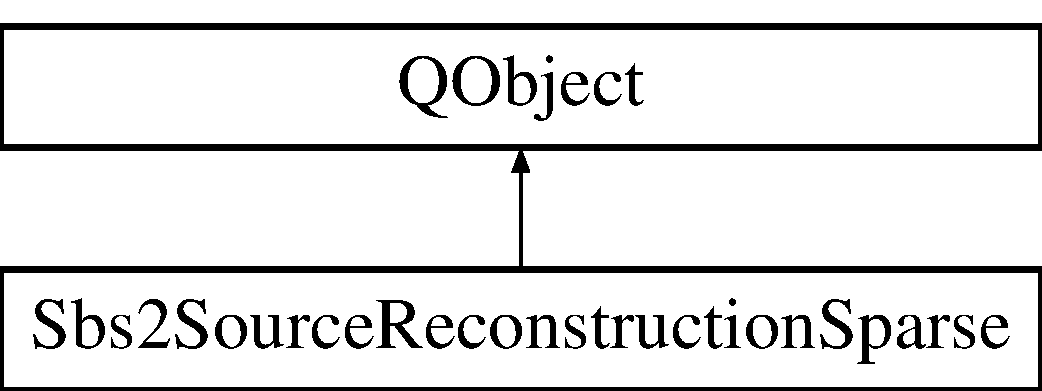
\includegraphics[height=2.000000cm]{classSbs2SourceReconstructionSparse}
\end{center}
\end{figure}
\subsection*{Public Member Functions}
\begin{DoxyCompactItemize}
\item 
\hyperlink{classSbs2SourceReconstructionSparse_ab51a1e6f1836882079c63792d79b475a}{Sbs2\-Source\-Reconstruction\-Sparse} (int channels\-\_\-input, int sources\-\_\-input, int samples\-\_\-, Q\-Vector$<$ double $>$ lambdas\-\_\-, Q\-String hardware\-\_\-, Q\-Object $\ast$parent=0, int num\-Datos\-Train\-\_\-input=8, int num\-Datos\-Test\-\_\-input=6, double error\-\_\-tol\-\_\-=0.\-0001)
\item 
void \hyperlink{classSbs2SourceReconstructionSparse_a7ce38152947515d6823d27366d708e58}{f\-\_\-objective\-\_\-general\-\_\-group\-\_\-lasso} (\hyperlink{classDTU_1_1DtuArray2D}{D\-T\-U\-::\-Dtu\-Array2\-D}$<$ double $>$ $\ast$A\-\_\-normalized, \hyperlink{classDTU_1_1DtuArray2D}{D\-T\-U\-::\-Dtu\-Array2\-D}$<$ double $>$ $\ast$S, \hyperlink{classDTU_1_1DtuArray2D}{D\-T\-U\-::\-Dtu\-Array2\-D}$<$ double $>$ $\ast$Y, double lambda, double $\ast$out)
\item 
void \hyperlink{classSbs2SourceReconstructionSparse_a37faa1ccf1cd9e4f5c505291b01679e3}{derivative\-\_\-square\-\_\-loss\-\_\-frobenius} (\hyperlink{classDTU_1_1DtuArray2D}{D\-T\-U\-::\-Dtu\-Array2\-D}$<$ double $>$ $\ast$A, \hyperlink{classDTU_1_1DtuArray2D}{D\-T\-U\-::\-Dtu\-Array2\-D}$<$ double $>$ $\ast$Y, \hyperlink{classDTU_1_1DtuArray2D}{D\-T\-U\-::\-Dtu\-Array2\-D}$<$ double $>$ $\ast$S, \hyperlink{classDTU_1_1DtuArray2D}{D\-T\-U\-::\-Dtu\-Array2\-D}$<$ double $>$ $\ast$out)
\item 
void \hyperlink{classSbs2SourceReconstructionSparse_ab65afe0fe91f8f79bfcfeb678b4dedfa}{proximal\-\_\-operator\-\_\-standard\-\_\-group\-\_\-lasso} (\hyperlink{classDTU_1_1DtuArray2D}{D\-T\-U\-::\-Dtu\-Array2\-D}$<$ double $>$ $\ast$X, double $\ast$regularizer\-\_\-factor, \hyperlink{classDTU_1_1DtuArray2D}{D\-T\-U\-::\-Dtu\-Array2\-D}$<$ double $>$ $\ast$out)
\item 
void \hyperlink{classSbs2SourceReconstructionSparse_a305baa833a5487152f006781ae563ec9}{fista\-\_\-method\-\_\-group\-\_\-lasso\-\_\-v2} (\hyperlink{classDTU_1_1DtuArray2D}{D\-T\-U\-::\-Dtu\-Array2\-D}$<$ double $>$ $\ast$A\-\_\-normalized, \hyperlink{classDTU_1_1DtuArray2D}{D\-T\-U\-::\-Dtu\-Array2\-D}$<$ double $>$ $\ast$Y, double lambda, double L, \hyperlink{classDTU_1_1DtuArray2D}{D\-T\-U\-::\-Dtu\-Array2\-D}$<$ double $>$ $\ast$estimated\-\_\-\-S)
\item 
void \hyperlink{classSbs2SourceReconstructionSparse_ae4fa7617ed4e1b06991ce00da77d3dae}{cross\-\_\-validation\-\_\-k\-\_\-channel} (\hyperlink{classDTU_1_1DtuArray2D}{D\-T\-U\-::\-Dtu\-Array2\-D}$<$ double $>$ $\ast$Y\-\_\-mean\-\_\-0, \hyperlink{classDTU_1_1DtuArray2D}{D\-T\-U\-::\-Dtu\-Array2\-D}$<$ double $>$ $\ast$estimated\-\_\-\-S)
\item 
void \hyperlink{classSbs2SourceReconstructionSparse_ae18dc4db1615715a25cf07085c76c9ca}{root\-Mean\-Square\-Error} (\hyperlink{classDTU_1_1DtuArray2D}{D\-T\-U\-::\-Dtu\-Array2\-D}$<$ double $>$ $\ast$Y\-\_\-mean\-\_\-0\-\_\-test, \hyperlink{classDTU_1_1DtuArray2D}{D\-T\-U\-::\-Dtu\-Array2\-D}$<$ double $>$ $\ast$A\-\_\-normalized\-\_\-test, \hyperlink{classDTU_1_1DtuArray2D}{D\-T\-U\-::\-Dtu\-Array2\-D}$<$ double $>$ $\ast$estimated\-\_\-\-S, double $\ast$rmse)
\item 
void \hyperlink{classSbs2SourceReconstructionSparse_a715684d11b00b3fbeba117730bbfe7ae}{do\-Rec} (\hyperlink{classDTU_1_1DtuArray2D}{D\-T\-U\-::\-Dtu\-Array2\-D}$<$ double $>$ $\ast$Y\-\_\-input, \hyperlink{classDTU_1_1DtuArray2D}{D\-T\-U\-::\-Dtu\-Array2\-D}$<$ double $>$ $\ast$S\-\_\-output, int $\ast$is\-Source\-Reconstruction\-Ready)
\item 
void \hyperlink{classSbs2SourceReconstructionSparse_af444570b73ff117a96a2555e57209616}{do\-Rec\-Pow} (\hyperlink{classDTU_1_1DtuArray2D}{D\-T\-U\-::\-Dtu\-Array2\-D}$<$ double $>$ $\ast$Y\-\_\-input, \hyperlink{classDTU_1_1DtuArray2D}{D\-T\-U\-::\-Dtu\-Array2\-D}$<$ double $>$ $\ast$S\-\_\-output, int $\ast$is\-Source\-Reconstruction\-Ready)
\item 
void \hyperlink{classSbs2SourceReconstructionSparse_a1b1e7a6b575f2b73198d5a01f17775c8}{preprocess\-Data} ()
\item 
void \hyperlink{classSbs2SourceReconstructionSparse_a63f21863593eea269b4bbba988872213}{calculate\-Mean} (\hyperlink{classDTU_1_1DtuArray2D}{D\-T\-U\-::\-Dtu\-Array2\-D}$<$ double $>$ $\ast$input, \hyperlink{classDTU_1_1DtuArray2D}{D\-T\-U\-::\-Dtu\-Array2\-D}$<$ double $>$ $\ast$output)
\item 
void \hyperlink{classSbs2SourceReconstructionSparse_a04505e279c6030ac70461aa7abf551d2}{calculate\-Power} (\hyperlink{classDTU_1_1DtuArray2D}{D\-T\-U\-::\-Dtu\-Array2\-D}$<$ double $>$ $\ast$input, \hyperlink{classDTU_1_1DtuArray2D}{D\-T\-U\-::\-Dtu\-Array2\-D}$<$ double $>$ $\ast$output)
\end{DoxyCompactItemize}


\subsection{Detailed Description}
Smartphone Brain Scanner 2 License Agreement (M\-I\-T License)

Copyright (c) 2012 Arkadiusz Stopczynski, Jakob Eg Larsen, Carsten Stahlhut, Michael Kai Petersen, Lars Kai Hansen. Technical University of Denmark, \hyperlink{namespaceDTU}{D\-T\-U} Informatics, Cognitive Systems Section. \href{http://code.google.com/p/smartphonebrainscanner2}{\tt http\-://code.\-google.\-com/p/smartphonebrainscanner2}

Permission is hereby granted, free of charge, to any person obtaining a copy of this software and associated documentation files (the \char`\"{}\-Software\char`\"{}), to deal in the Software without restriction, including without limitation the rights to use, copy, modify, merge, publish, distribute, sublicense, and/or sell copies of the Software, and to permit persons to whom the Software is furnished to do so, subject to the following conditions\-:

The above copyright notice and this permission notice shall be included in all copies or substantial portions of the Software.

T\-H\-E S\-O\-F\-T\-W\-A\-R\-E I\-S P\-R\-O\-V\-I\-D\-E\-D \char`\"{}\-A\-S I\-S\char`\"{}, W\-I\-T\-H\-O\-U\-T W\-A\-R\-R\-A\-N\-T\-Y O\-F A\-N\-Y K\-I\-N\-D, E\-X\-P\-R\-E\-S\-S O\-R I\-M\-P\-L\-I\-E\-D, I\-N\-C\-L\-U\-D\-I\-N\-G B\-U\-T N\-O\-T L\-I\-M\-I\-T\-E\-D T\-O T\-H\-E W\-A\-R\-R\-A\-N\-T\-I\-E\-S O\-F M\-E\-R\-C\-H\-A\-N\-T\-A\-B\-I\-L\-I\-T\-Y, F\-I\-T\-N\-E\-S\-S F\-O\-R A P\-A\-R\-T\-I\-C\-U\-L\-A\-R P\-U\-R\-P\-O\-S\-E A\-N\-D N\-O\-N\-I\-N\-F\-R\-I\-N\-G\-E\-M\-E\-N\-T. I\-N N\-O E\-V\-E\-N\-T S\-H\-A\-L\-L T\-H\-E A\-U\-T\-H\-O\-R\-S O\-R C\-O\-P\-Y\-R\-I\-G\-H\-T H\-O\-L\-D\-E\-R\-S B\-E L\-I\-A\-B\-L\-E F\-O\-R A\-N\-Y C\-L\-A\-I\-M, D\-A\-M\-A\-G\-E\-S O\-R O\-T\-H\-E\-R L\-I\-A\-B\-I\-L\-I\-T\-Y, W\-H\-E\-T\-H\-E\-R I\-N A\-N A\-C\-T\-I\-O\-N O\-F C\-O\-N\-T\-R\-A\-C\-T, T\-O\-R\-T O\-R O\-T\-H\-E\-R\-W\-I\-S\-E, A\-R\-I\-S\-I\-N\-G F\-R\-O\-M, O\-U\-T O\-F O\-R I\-N C\-O\-N\-N\-E\-C\-T\-I\-O\-N W\-I\-T\-H T\-H\-E S\-O\-F\-T\-W\-A\-R\-E O\-R T\-H\-E U\-S\-E O\-R O\-T\-H\-E\-R D\-E\-A\-L\-I\-N\-G\-S I\-N T\-H\-E S\-O\-F\-T\-W\-A\-R\-E. 

\subsection{Constructor \& Destructor Documentation}
\hypertarget{classSbs2SourceReconstructionSparse_ab51a1e6f1836882079c63792d79b475a}{\index{Sbs2\-Source\-Reconstruction\-Sparse@{Sbs2\-Source\-Reconstruction\-Sparse}!Sbs2\-Source\-Reconstruction\-Sparse@{Sbs2\-Source\-Reconstruction\-Sparse}}
\index{Sbs2\-Source\-Reconstruction\-Sparse@{Sbs2\-Source\-Reconstruction\-Sparse}!Sbs2SourceReconstructionSparse@{Sbs2\-Source\-Reconstruction\-Sparse}}
\subsubsection[{Sbs2\-Source\-Reconstruction\-Sparse}]{\setlength{\rightskip}{0pt plus 5cm}Sbs2\-Source\-Reconstruction\-Sparse\-::\-Sbs2\-Source\-Reconstruction\-Sparse (
\begin{DoxyParamCaption}
\item[{int}]{channels\-\_\-input, }
\item[{int}]{sources\-\_\-input, }
\item[{int}]{samples\-\_\-, }
\item[{Q\-Vector$<$ double $>$}]{lambdas\-\_\-, }
\item[{Q\-String}]{hardware\-\_\-, }
\item[{Q\-Object $\ast$}]{parent = {\ttfamily 0}, }
\item[{int}]{num\-Datos\-Train\-\_\-input = {\ttfamily 8}, }
\item[{int}]{num\-Datos\-Test\-\_\-input = {\ttfamily 6}, }
\item[{double}]{error\-\_\-tol\-\_\- = {\ttfamily 0.0001}}
\end{DoxyParamCaption}
)\hspace{0.3cm}{\ttfamily [explicit]}}}\label{classSbs2SourceReconstructionSparse_ab51a1e6f1836882079c63792d79b475a}
Variables used in the function fista\-\_\-method\-\_\-group\-\_\-lasso\-\_\-v2 

\subsection{Member Function Documentation}
\hypertarget{classSbs2SourceReconstructionSparse_a63f21863593eea269b4bbba988872213}{\index{Sbs2\-Source\-Reconstruction\-Sparse@{Sbs2\-Source\-Reconstruction\-Sparse}!calculate\-Mean@{calculate\-Mean}}
\index{calculate\-Mean@{calculate\-Mean}!Sbs2SourceReconstructionSparse@{Sbs2\-Source\-Reconstruction\-Sparse}}
\subsubsection[{calculate\-Mean}]{\setlength{\rightskip}{0pt plus 5cm}void Sbs2\-Source\-Reconstruction\-Sparse\-::calculate\-Mean (
\begin{DoxyParamCaption}
\item[{{\bf D\-T\-U\-::\-Dtu\-Array2\-D}$<$ double $>$ $\ast$}]{input, }
\item[{{\bf D\-T\-U\-::\-Dtu\-Array2\-D}$<$ double $>$ $\ast$}]{output}
\end{DoxyParamCaption}
)}}\label{classSbs2SourceReconstructionSparse_a63f21863593eea269b4bbba988872213}
\hypertarget{classSbs2SourceReconstructionSparse_a04505e279c6030ac70461aa7abf551d2}{\index{Sbs2\-Source\-Reconstruction\-Sparse@{Sbs2\-Source\-Reconstruction\-Sparse}!calculate\-Power@{calculate\-Power}}
\index{calculate\-Power@{calculate\-Power}!Sbs2SourceReconstructionSparse@{Sbs2\-Source\-Reconstruction\-Sparse}}
\subsubsection[{calculate\-Power}]{\setlength{\rightskip}{0pt plus 5cm}void Sbs2\-Source\-Reconstruction\-Sparse\-::calculate\-Power (
\begin{DoxyParamCaption}
\item[{{\bf D\-T\-U\-::\-Dtu\-Array2\-D}$<$ double $>$ $\ast$}]{input, }
\item[{{\bf D\-T\-U\-::\-Dtu\-Array2\-D}$<$ double $>$ $\ast$}]{output}
\end{DoxyParamCaption}
)}}\label{classSbs2SourceReconstructionSparse_a04505e279c6030ac70461aa7abf551d2}
\hypertarget{classSbs2SourceReconstructionSparse_ae4fa7617ed4e1b06991ce00da77d3dae}{\index{Sbs2\-Source\-Reconstruction\-Sparse@{Sbs2\-Source\-Reconstruction\-Sparse}!cross\-\_\-validation\-\_\-k\-\_\-channel@{cross\-\_\-validation\-\_\-k\-\_\-channel}}
\index{cross\-\_\-validation\-\_\-k\-\_\-channel@{cross\-\_\-validation\-\_\-k\-\_\-channel}!Sbs2SourceReconstructionSparse@{Sbs2\-Source\-Reconstruction\-Sparse}}
\subsubsection[{cross\-\_\-validation\-\_\-k\-\_\-channel}]{\setlength{\rightskip}{0pt plus 5cm}void Sbs2\-Source\-Reconstruction\-Sparse\-::cross\-\_\-validation\-\_\-k\-\_\-channel (
\begin{DoxyParamCaption}
\item[{{\bf D\-T\-U\-::\-Dtu\-Array2\-D}$<$ double $>$ $\ast$}]{Y\-\_\-mean\-\_\-0, }
\item[{{\bf D\-T\-U\-::\-Dtu\-Array2\-D}$<$ double $>$ $\ast$}]{estimated\-\_\-\-S}
\end{DoxyParamCaption}
)}}\label{classSbs2SourceReconstructionSparse_ae4fa7617ed4e1b06991ce00da77d3dae}
\hypertarget{classSbs2SourceReconstructionSparse_a37faa1ccf1cd9e4f5c505291b01679e3}{\index{Sbs2\-Source\-Reconstruction\-Sparse@{Sbs2\-Source\-Reconstruction\-Sparse}!derivative\-\_\-square\-\_\-loss\-\_\-frobenius@{derivative\-\_\-square\-\_\-loss\-\_\-frobenius}}
\index{derivative\-\_\-square\-\_\-loss\-\_\-frobenius@{derivative\-\_\-square\-\_\-loss\-\_\-frobenius}!Sbs2SourceReconstructionSparse@{Sbs2\-Source\-Reconstruction\-Sparse}}
\subsubsection[{derivative\-\_\-square\-\_\-loss\-\_\-frobenius}]{\setlength{\rightskip}{0pt plus 5cm}void Sbs2\-Source\-Reconstruction\-Sparse\-::derivative\-\_\-square\-\_\-loss\-\_\-frobenius (
\begin{DoxyParamCaption}
\item[{{\bf D\-T\-U\-::\-Dtu\-Array2\-D}$<$ double $>$ $\ast$}]{A, }
\item[{{\bf D\-T\-U\-::\-Dtu\-Array2\-D}$<$ double $>$ $\ast$}]{Y, }
\item[{{\bf D\-T\-U\-::\-Dtu\-Array2\-D}$<$ double $>$ $\ast$}]{S, }
\item[{{\bf D\-T\-U\-::\-Dtu\-Array2\-D}$<$ double $>$ $\ast$}]{out}
\end{DoxyParamCaption}
)}}\label{classSbs2SourceReconstructionSparse_a37faa1ccf1cd9e4f5c505291b01679e3}
\hypertarget{classSbs2SourceReconstructionSparse_a715684d11b00b3fbeba117730bbfe7ae}{\index{Sbs2\-Source\-Reconstruction\-Sparse@{Sbs2\-Source\-Reconstruction\-Sparse}!do\-Rec@{do\-Rec}}
\index{do\-Rec@{do\-Rec}!Sbs2SourceReconstructionSparse@{Sbs2\-Source\-Reconstruction\-Sparse}}
\subsubsection[{do\-Rec}]{\setlength{\rightskip}{0pt plus 5cm}void Sbs2\-Source\-Reconstruction\-Sparse\-::do\-Rec (
\begin{DoxyParamCaption}
\item[{{\bf D\-T\-U\-::\-Dtu\-Array2\-D}$<$ double $>$ $\ast$}]{Y\-\_\-input, }
\item[{{\bf D\-T\-U\-::\-Dtu\-Array2\-D}$<$ double $>$ $\ast$}]{S\-\_\-output, }
\item[{int $\ast$}]{is\-Source\-Reconstruction\-Ready}
\end{DoxyParamCaption}
)}}\label{classSbs2SourceReconstructionSparse_a715684d11b00b3fbeba117730bbfe7ae}
\hypertarget{classSbs2SourceReconstructionSparse_af444570b73ff117a96a2555e57209616}{\index{Sbs2\-Source\-Reconstruction\-Sparse@{Sbs2\-Source\-Reconstruction\-Sparse}!do\-Rec\-Pow@{do\-Rec\-Pow}}
\index{do\-Rec\-Pow@{do\-Rec\-Pow}!Sbs2SourceReconstructionSparse@{Sbs2\-Source\-Reconstruction\-Sparse}}
\subsubsection[{do\-Rec\-Pow}]{\setlength{\rightskip}{0pt plus 5cm}void Sbs2\-Source\-Reconstruction\-Sparse\-::do\-Rec\-Pow (
\begin{DoxyParamCaption}
\item[{{\bf D\-T\-U\-::\-Dtu\-Array2\-D}$<$ double $>$ $\ast$}]{Y\-\_\-input, }
\item[{{\bf D\-T\-U\-::\-Dtu\-Array2\-D}$<$ double $>$ $\ast$}]{S\-\_\-output, }
\item[{int $\ast$}]{is\-Source\-Reconstruction\-Ready}
\end{DoxyParamCaption}
)}}\label{classSbs2SourceReconstructionSparse_af444570b73ff117a96a2555e57209616}
\hypertarget{classSbs2SourceReconstructionSparse_a7ce38152947515d6823d27366d708e58}{\index{Sbs2\-Source\-Reconstruction\-Sparse@{Sbs2\-Source\-Reconstruction\-Sparse}!f\-\_\-objective\-\_\-general\-\_\-group\-\_\-lasso@{f\-\_\-objective\-\_\-general\-\_\-group\-\_\-lasso}}
\index{f\-\_\-objective\-\_\-general\-\_\-group\-\_\-lasso@{f\-\_\-objective\-\_\-general\-\_\-group\-\_\-lasso}!Sbs2SourceReconstructionSparse@{Sbs2\-Source\-Reconstruction\-Sparse}}
\subsubsection[{f\-\_\-objective\-\_\-general\-\_\-group\-\_\-lasso}]{\setlength{\rightskip}{0pt plus 5cm}void Sbs2\-Source\-Reconstruction\-Sparse\-::f\-\_\-objective\-\_\-general\-\_\-group\-\_\-lasso (
\begin{DoxyParamCaption}
\item[{{\bf D\-T\-U\-::\-Dtu\-Array2\-D}$<$ double $>$ $\ast$}]{A\-\_\-normalized, }
\item[{{\bf D\-T\-U\-::\-Dtu\-Array2\-D}$<$ double $>$ $\ast$}]{S, }
\item[{{\bf D\-T\-U\-::\-Dtu\-Array2\-D}$<$ double $>$ $\ast$}]{Y, }
\item[{double}]{lambda, }
\item[{double $\ast$}]{out}
\end{DoxyParamCaption}
)}}\label{classSbs2SourceReconstructionSparse_a7ce38152947515d6823d27366d708e58}
\hypertarget{classSbs2SourceReconstructionSparse_a305baa833a5487152f006781ae563ec9}{\index{Sbs2\-Source\-Reconstruction\-Sparse@{Sbs2\-Source\-Reconstruction\-Sparse}!fista\-\_\-method\-\_\-group\-\_\-lasso\-\_\-v2@{fista\-\_\-method\-\_\-group\-\_\-lasso\-\_\-v2}}
\index{fista\-\_\-method\-\_\-group\-\_\-lasso\-\_\-v2@{fista\-\_\-method\-\_\-group\-\_\-lasso\-\_\-v2}!Sbs2SourceReconstructionSparse@{Sbs2\-Source\-Reconstruction\-Sparse}}
\subsubsection[{fista\-\_\-method\-\_\-group\-\_\-lasso\-\_\-v2}]{\setlength{\rightskip}{0pt plus 5cm}void Sbs2\-Source\-Reconstruction\-Sparse\-::fista\-\_\-method\-\_\-group\-\_\-lasso\-\_\-v2 (
\begin{DoxyParamCaption}
\item[{{\bf D\-T\-U\-::\-Dtu\-Array2\-D}$<$ double $>$ $\ast$}]{A\-\_\-normalized, }
\item[{{\bf D\-T\-U\-::\-Dtu\-Array2\-D}$<$ double $>$ $\ast$}]{Y, }
\item[{double}]{lambda, }
\item[{double}]{L, }
\item[{{\bf D\-T\-U\-::\-Dtu\-Array2\-D}$<$ double $>$ $\ast$}]{estimated\-\_\-\-S}
\end{DoxyParamCaption}
)}}\label{classSbs2SourceReconstructionSparse_a305baa833a5487152f006781ae563ec9}
\hypertarget{classSbs2SourceReconstructionSparse_a1b1e7a6b575f2b73198d5a01f17775c8}{\index{Sbs2\-Source\-Reconstruction\-Sparse@{Sbs2\-Source\-Reconstruction\-Sparse}!preprocess\-Data@{preprocess\-Data}}
\index{preprocess\-Data@{preprocess\-Data}!Sbs2SourceReconstructionSparse@{Sbs2\-Source\-Reconstruction\-Sparse}}
\subsubsection[{preprocess\-Data}]{\setlength{\rightskip}{0pt plus 5cm}void Sbs2\-Source\-Reconstruction\-Sparse\-::preprocess\-Data (
\begin{DoxyParamCaption}
{}
\end{DoxyParamCaption}
)}}\label{classSbs2SourceReconstructionSparse_a1b1e7a6b575f2b73198d5a01f17775c8}
\hypertarget{classSbs2SourceReconstructionSparse_ab65afe0fe91f8f79bfcfeb678b4dedfa}{\index{Sbs2\-Source\-Reconstruction\-Sparse@{Sbs2\-Source\-Reconstruction\-Sparse}!proximal\-\_\-operator\-\_\-standard\-\_\-group\-\_\-lasso@{proximal\-\_\-operator\-\_\-standard\-\_\-group\-\_\-lasso}}
\index{proximal\-\_\-operator\-\_\-standard\-\_\-group\-\_\-lasso@{proximal\-\_\-operator\-\_\-standard\-\_\-group\-\_\-lasso}!Sbs2SourceReconstructionSparse@{Sbs2\-Source\-Reconstruction\-Sparse}}
\subsubsection[{proximal\-\_\-operator\-\_\-standard\-\_\-group\-\_\-lasso}]{\setlength{\rightskip}{0pt plus 5cm}void Sbs2\-Source\-Reconstruction\-Sparse\-::proximal\-\_\-operator\-\_\-standard\-\_\-group\-\_\-lasso (
\begin{DoxyParamCaption}
\item[{{\bf D\-T\-U\-::\-Dtu\-Array2\-D}$<$ double $>$ $\ast$}]{X, }
\item[{double $\ast$}]{regularizer\-\_\-factor, }
\item[{{\bf D\-T\-U\-::\-Dtu\-Array2\-D}$<$ double $>$ $\ast$}]{out}
\end{DoxyParamCaption}
)}}\label{classSbs2SourceReconstructionSparse_ab65afe0fe91f8f79bfcfeb678b4dedfa}
\hypertarget{classSbs2SourceReconstructionSparse_ae18dc4db1615715a25cf07085c76c9ca}{\index{Sbs2\-Source\-Reconstruction\-Sparse@{Sbs2\-Source\-Reconstruction\-Sparse}!root\-Mean\-Square\-Error@{root\-Mean\-Square\-Error}}
\index{root\-Mean\-Square\-Error@{root\-Mean\-Square\-Error}!Sbs2SourceReconstructionSparse@{Sbs2\-Source\-Reconstruction\-Sparse}}
\subsubsection[{root\-Mean\-Square\-Error}]{\setlength{\rightskip}{0pt plus 5cm}void Sbs2\-Source\-Reconstruction\-Sparse\-::root\-Mean\-Square\-Error (
\begin{DoxyParamCaption}
\item[{{\bf D\-T\-U\-::\-Dtu\-Array2\-D}$<$ double $>$ $\ast$}]{Y\-\_\-mean\-\_\-0\-\_\-test, }
\item[{{\bf D\-T\-U\-::\-Dtu\-Array2\-D}$<$ double $>$ $\ast$}]{A\-\_\-normalized\-\_\-test, }
\item[{{\bf D\-T\-U\-::\-Dtu\-Array2\-D}$<$ double $>$ $\ast$}]{estimated\-\_\-\-S, }
\item[{double $\ast$}]{rmse}
\end{DoxyParamCaption}
)}}\label{classSbs2SourceReconstructionSparse_ae18dc4db1615715a25cf07085c76c9ca}


The documentation for this class was generated from the following files\-:\begin{DoxyCompactItemize}
\item 
/media/philipjhj/\-Data/\-One\-Drive/\-Studie/\-Studenterprogrammør/\-S\-B\-S3/smartphonebrainscanner2-\/core/src/source\-\_\-reconstruction/sparse/\hyperlink{sbs2sourcereconstruction__sparse_8h}{sbs2sourcereconstruction\-\_\-sparse.\-h}\item 
/media/philipjhj/\-Data/\-One\-Drive/\-Studie/\-Studenterprogrammør/\-S\-B\-S3/smartphonebrainscanner2-\/core/src/source\-\_\-reconstruction/sparse/\hyperlink{sbs2sourcereconstruction__sparse_8cpp}{sbs2sourcereconstruction\-\_\-sparse.\-cpp}\end{DoxyCompactItemize}

\hypertarget{classSbs2Spectrogram}{\section{Sbs2\-Spectrogram Class Reference}
\label{classSbs2Spectrogram}\index{Sbs2\-Spectrogram@{Sbs2\-Spectrogram}}
}


{\ttfamily \#include $<$sbs2spectrogram.\-h$>$}

Inheritance diagram for Sbs2\-Spectrogram\-:\begin{figure}[H]
\begin{center}
\leavevmode
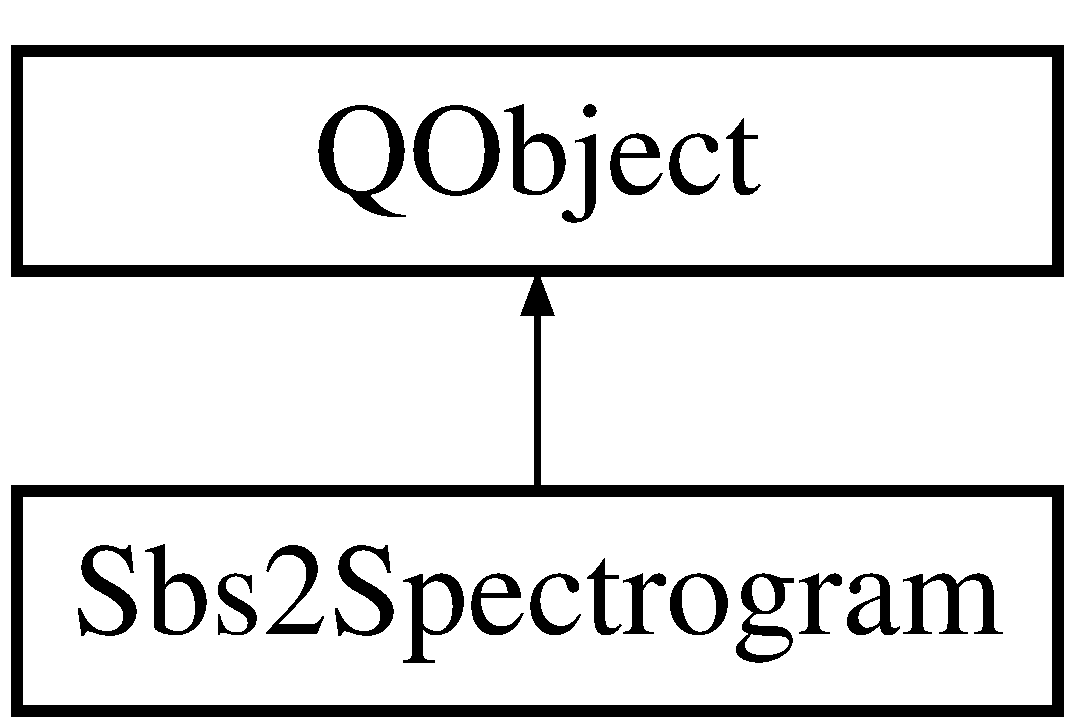
\includegraphics[height=2.000000cm]{classSbs2Spectrogram}
\end{center}
\end{figure}
\subsection*{Public Types}
\begin{DoxyCompactItemize}
\item 
enum \hyperlink{classSbs2Spectrogram_a22265347883488b8385c83b67882d915}{Window\-Type} \{ \hyperlink{classSbs2Spectrogram_a22265347883488b8385c83b67882d915a53cead410460e1e97357918fb4551295}{R\-E\-C\-T}, 
\hyperlink{classSbs2Spectrogram_a22265347883488b8385c83b67882d915aedef05928888024ac640151a903ccd65}{H\-A\-N\-N}, 
\hyperlink{classSbs2Spectrogram_a22265347883488b8385c83b67882d915afcbd3c1363abfd250fad7cf50af578ff}{H\-A\-M\-M\-I\-N\-G}
 \}
\end{DoxyCompactItemize}
\subsection*{Public Slots}
\begin{DoxyCompactItemize}
\item 
void \hyperlink{classSbs2Spectrogram_aba3b9a1d6685a23737cf44f21a9dd57f}{set\-Window\-Type} (\hyperlink{classSbs2Spectrogram_a22265347883488b8385c83b67882d915}{Sbs2\-Spectrogram\-::\-Window\-Type} window\-Type\-\_\-)
\end{DoxyCompactItemize}
\subsection*{Public Member Functions}
\begin{DoxyCompactItemize}
\item 
\hyperlink{classSbs2Spectrogram_a5093d21393080d54dd3c8ce7e198a204}{Sbs2\-Spectrogram} (int length\-\_\-, Q\-Object $\ast$parent=0)
\item 
void \hyperlink{classSbs2Spectrogram_ae2e56ca4415a47a1b52464d94a6c228b}{do\-Spectrogram} (\hyperlink{classDTU_1_1DtuArray2D}{D\-T\-U\-::\-Dtu\-Array2\-D}$<$ double $>$ $\ast$input, \hyperlink{classDTU_1_1DtuArray2D}{D\-T\-U\-::\-Dtu\-Array2\-D}$<$ double $>$ $\ast$output)
\item 
\hyperlink{classSbs2Spectrogram_a377a6b3e8f5e9414799c9104f8e5b3c8}{$\sim$\-Sbs2\-Spectrogram} ()
\item 
\hyperlink{classSbs2Spectrogram_a22265347883488b8385c83b67882d915}{Window\-Type} \hyperlink{classSbs2Spectrogram_ae46ac1ab353d0110cb121971e6cb5140}{get\-Window\-Type} ()
\end{DoxyCompactItemize}


\subsection{Member Enumeration Documentation}
\hypertarget{classSbs2Spectrogram_a22265347883488b8385c83b67882d915}{\index{Sbs2\-Spectrogram@{Sbs2\-Spectrogram}!Window\-Type@{Window\-Type}}
\index{Window\-Type@{Window\-Type}!Sbs2Spectrogram@{Sbs2\-Spectrogram}}
\subsubsection[{Window\-Type}]{\setlength{\rightskip}{0pt plus 5cm}enum {\bf Sbs2\-Spectrogram\-::\-Window\-Type}}}\label{classSbs2Spectrogram_a22265347883488b8385c83b67882d915}
\begin{Desc}
\item[Enumerator]\par
\begin{description}
\index{R\-E\-C\-T@{R\-E\-C\-T}!Sbs2\-Spectrogram@{Sbs2\-Spectrogram}}\index{Sbs2\-Spectrogram@{Sbs2\-Spectrogram}!R\-E\-C\-T@{R\-E\-C\-T}}\item[{\em 
\hypertarget{classSbs2Spectrogram_a22265347883488b8385c83b67882d915a53cead410460e1e97357918fb4551295}{R\-E\-C\-T}\label{classSbs2Spectrogram_a22265347883488b8385c83b67882d915a53cead410460e1e97357918fb4551295}
}]\index{H\-A\-N\-N@{H\-A\-N\-N}!Sbs2\-Spectrogram@{Sbs2\-Spectrogram}}\index{Sbs2\-Spectrogram@{Sbs2\-Spectrogram}!H\-A\-N\-N@{H\-A\-N\-N}}\item[{\em 
\hypertarget{classSbs2Spectrogram_a22265347883488b8385c83b67882d915aedef05928888024ac640151a903ccd65}{H\-A\-N\-N}\label{classSbs2Spectrogram_a22265347883488b8385c83b67882d915aedef05928888024ac640151a903ccd65}
}]\index{H\-A\-M\-M\-I\-N\-G@{H\-A\-M\-M\-I\-N\-G}!Sbs2\-Spectrogram@{Sbs2\-Spectrogram}}\index{Sbs2\-Spectrogram@{Sbs2\-Spectrogram}!H\-A\-M\-M\-I\-N\-G@{H\-A\-M\-M\-I\-N\-G}}\item[{\em 
\hypertarget{classSbs2Spectrogram_a22265347883488b8385c83b67882d915afcbd3c1363abfd250fad7cf50af578ff}{H\-A\-M\-M\-I\-N\-G}\label{classSbs2Spectrogram_a22265347883488b8385c83b67882d915afcbd3c1363abfd250fad7cf50af578ff}
}]\end{description}
\end{Desc}


\subsection{Constructor \& Destructor Documentation}
\hypertarget{classSbs2Spectrogram_a5093d21393080d54dd3c8ce7e198a204}{\index{Sbs2\-Spectrogram@{Sbs2\-Spectrogram}!Sbs2\-Spectrogram@{Sbs2\-Spectrogram}}
\index{Sbs2\-Spectrogram@{Sbs2\-Spectrogram}!Sbs2Spectrogram@{Sbs2\-Spectrogram}}
\subsubsection[{Sbs2\-Spectrogram}]{\setlength{\rightskip}{0pt plus 5cm}Sbs2\-Spectrogram\-::\-Sbs2\-Spectrogram (
\begin{DoxyParamCaption}
\item[{int}]{length\-\_\-, }
\item[{Q\-Object $\ast$}]{parent = {\ttfamily 0}}
\end{DoxyParamCaption}
)\hspace{0.3cm}{\ttfamily [explicit]}}}\label{classSbs2Spectrogram_a5093d21393080d54dd3c8ce7e198a204}
\hypertarget{classSbs2Spectrogram_a377a6b3e8f5e9414799c9104f8e5b3c8}{\index{Sbs2\-Spectrogram@{Sbs2\-Spectrogram}!$\sim$\-Sbs2\-Spectrogram@{$\sim$\-Sbs2\-Spectrogram}}
\index{$\sim$\-Sbs2\-Spectrogram@{$\sim$\-Sbs2\-Spectrogram}!Sbs2Spectrogram@{Sbs2\-Spectrogram}}
\subsubsection[{$\sim$\-Sbs2\-Spectrogram}]{\setlength{\rightskip}{0pt plus 5cm}Sbs2\-Spectrogram\-::$\sim$\-Sbs2\-Spectrogram (
\begin{DoxyParamCaption}
{}
\end{DoxyParamCaption}
)}}\label{classSbs2Spectrogram_a377a6b3e8f5e9414799c9104f8e5b3c8}


\subsection{Member Function Documentation}
\hypertarget{classSbs2Spectrogram_ae2e56ca4415a47a1b52464d94a6c228b}{\index{Sbs2\-Spectrogram@{Sbs2\-Spectrogram}!do\-Spectrogram@{do\-Spectrogram}}
\index{do\-Spectrogram@{do\-Spectrogram}!Sbs2Spectrogram@{Sbs2\-Spectrogram}}
\subsubsection[{do\-Spectrogram}]{\setlength{\rightskip}{0pt plus 5cm}void Sbs2\-Spectrogram\-::do\-Spectrogram (
\begin{DoxyParamCaption}
\item[{{\bf D\-T\-U\-::\-Dtu\-Array2\-D}$<$ double $>$ $\ast$}]{input, }
\item[{{\bf D\-T\-U\-::\-Dtu\-Array2\-D}$<$ double $>$ $\ast$}]{output}
\end{DoxyParamCaption}
)}}\label{classSbs2Spectrogram_ae2e56ca4415a47a1b52464d94a6c228b}
\hypertarget{classSbs2Spectrogram_ae46ac1ab353d0110cb121971e6cb5140}{\index{Sbs2\-Spectrogram@{Sbs2\-Spectrogram}!get\-Window\-Type@{get\-Window\-Type}}
\index{get\-Window\-Type@{get\-Window\-Type}!Sbs2Spectrogram@{Sbs2\-Spectrogram}}
\subsubsection[{get\-Window\-Type}]{\setlength{\rightskip}{0pt plus 5cm}{\bf Sbs2\-Spectrogram\-::\-Window\-Type} Sbs2\-Spectrogram\-::get\-Window\-Type (
\begin{DoxyParamCaption}
{}
\end{DoxyParamCaption}
)}}\label{classSbs2Spectrogram_ae46ac1ab353d0110cb121971e6cb5140}
\hypertarget{classSbs2Spectrogram_aba3b9a1d6685a23737cf44f21a9dd57f}{\index{Sbs2\-Spectrogram@{Sbs2\-Spectrogram}!set\-Window\-Type@{set\-Window\-Type}}
\index{set\-Window\-Type@{set\-Window\-Type}!Sbs2Spectrogram@{Sbs2\-Spectrogram}}
\subsubsection[{set\-Window\-Type}]{\setlength{\rightskip}{0pt plus 5cm}void Sbs2\-Spectrogram\-::set\-Window\-Type (
\begin{DoxyParamCaption}
\item[{{\bf Sbs2\-Spectrogram\-::\-Window\-Type}}]{window\-Type\-\_\-}
\end{DoxyParamCaption}
)\hspace{0.3cm}{\ttfamily [slot]}}}\label{classSbs2Spectrogram_aba3b9a1d6685a23737cf44f21a9dd57f}


The documentation for this class was generated from the following files\-:\begin{DoxyCompactItemize}
\item 
/media/philipjhj/\-Data/\-One\-Drive/\-Studie/\-Studenterprogrammør/\-S\-B\-S3/smartphonebrainscanner2-\/core/src/\hyperlink{sbs2spectrogram_8h}{sbs2spectrogram.\-h}\item 
/media/philipjhj/\-Data/\-One\-Drive/\-Studie/\-Studenterprogrammør/\-S\-B\-S3/smartphonebrainscanner2-\/core/src/\hyperlink{sbs2spectrogram_8cpp}{sbs2spectrogram.\-cpp}\end{DoxyCompactItemize}

\hypertarget{classSbs2Timer}{\section{Sbs2\-Timer Class Reference}
\label{classSbs2Timer}\index{Sbs2\-Timer@{Sbs2\-Timer}}
}


{\ttfamily \#include $<$sbs2timer.\-h$>$}

Inheritance diagram for Sbs2\-Timer\-:\begin{figure}[H]
\begin{center}
\leavevmode
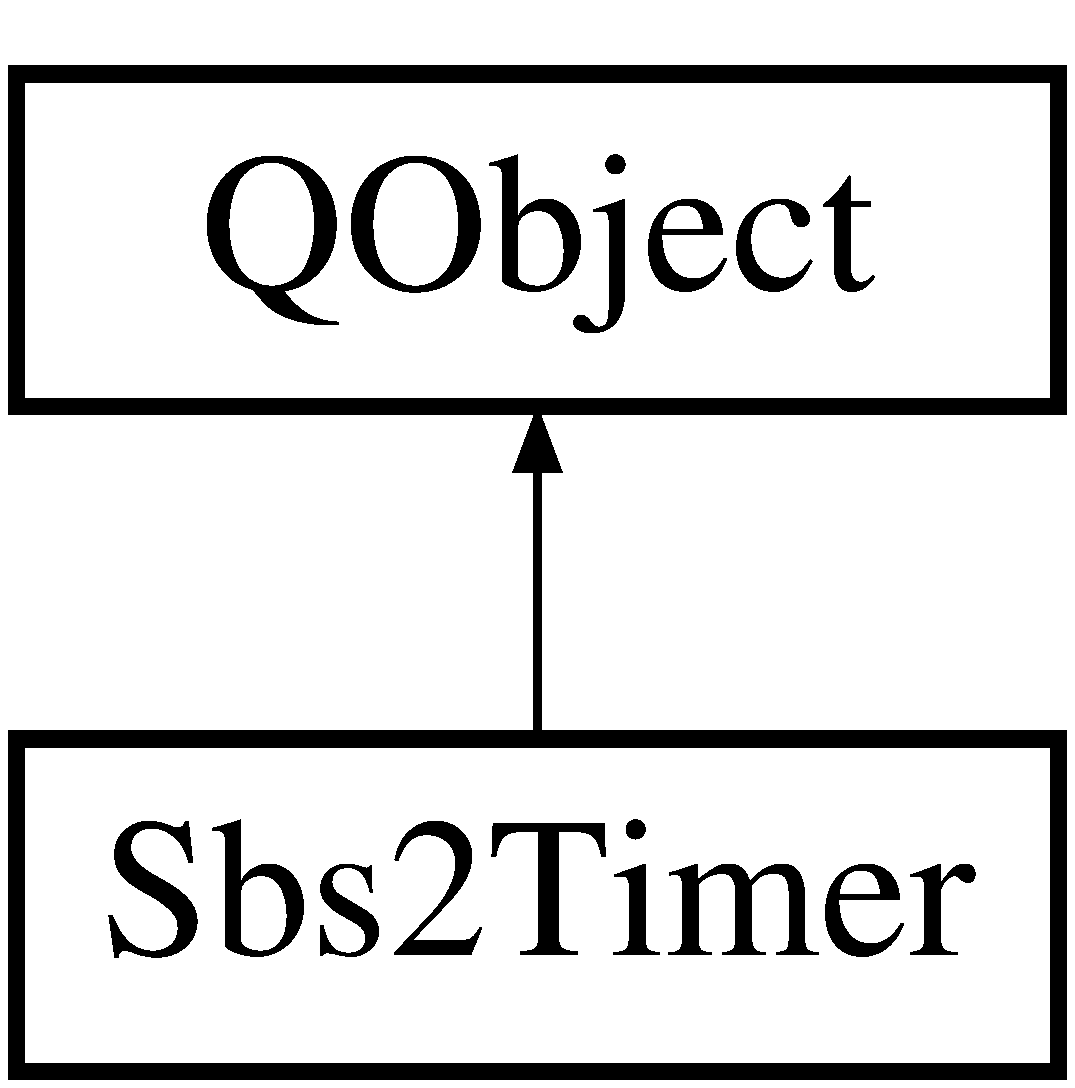
\includegraphics[height=2.000000cm]{classSbs2Timer}
\end{center}
\end{figure}
\subsection*{Public Member Functions}
\begin{DoxyCompactItemize}
\item 
\hyperlink{classSbs2Timer_ad7b35793f48ddcbd4a5fb14c5f277bd3}{Sbs2\-Timer} (Q\-Object $\ast$parent=0)
\end{DoxyCompactItemize}
\subsection*{Static Public Member Functions}
\begin{DoxyCompactItemize}
\item 
static void \hyperlink{classSbs2Timer_a496729d5514d8dd99b2d20f584c743e9}{tic} ()
\item 
static void \hyperlink{classSbs2Timer_a0316896c140e62155e45a0a5c3382432}{tic} (Q\-String label\-\_\-)
\item 
static void \hyperlink{classSbs2Timer_ac4a8bdc4eceb47ac9971425332eb7aee}{toc} ()
\end{DoxyCompactItemize}
\subsection*{Static Public Attributes}
\begin{DoxyCompactItemize}
\item 
static qint64 \hyperlink{classSbs2Timer_acd1e0853bb3a6e0477f86d5f00546c9a}{tic\-\_\-time} = 0
\end{DoxyCompactItemize}


\subsection{Detailed Description}
Smartphone Brain Scanner 2 License Agreement (M\-I\-T License)

Copyright (c) 2012 Arkadiusz Stopczynski, Jakob Eg Larsen, Carsten Stahlhut, Michael Kai Petersen, Lars Kai Hansen. Technical University of Denmark, \hyperlink{namespaceDTU}{D\-T\-U} Informatics, Cognitive Systems Section. \href{http://code.google.com/p/smartphonebrainscanner2}{\tt http\-://code.\-google.\-com/p/smartphonebrainscanner2}

Permission is hereby granted, free of charge, to any person obtaining a copy of this software and associated documentation files (the \char`\"{}\-Software\char`\"{}), to deal in the Software without restriction, including without limitation the rights to use, copy, modify, merge, publish, distribute, sublicense, and/or sell copies of the Software, and to permit persons to whom the Software is furnished to do so, subject to the following conditions\-:

The above copyright notice and this permission notice shall be included in all copies or substantial portions of the Software.

T\-H\-E S\-O\-F\-T\-W\-A\-R\-E I\-S P\-R\-O\-V\-I\-D\-E\-D \char`\"{}\-A\-S I\-S\char`\"{}, W\-I\-T\-H\-O\-U\-T W\-A\-R\-R\-A\-N\-T\-Y O\-F A\-N\-Y K\-I\-N\-D, E\-X\-P\-R\-E\-S\-S O\-R I\-M\-P\-L\-I\-E\-D, I\-N\-C\-L\-U\-D\-I\-N\-G B\-U\-T N\-O\-T L\-I\-M\-I\-T\-E\-D T\-O T\-H\-E W\-A\-R\-R\-A\-N\-T\-I\-E\-S O\-F M\-E\-R\-C\-H\-A\-N\-T\-A\-B\-I\-L\-I\-T\-Y, F\-I\-T\-N\-E\-S\-S F\-O\-R A P\-A\-R\-T\-I\-C\-U\-L\-A\-R P\-U\-R\-P\-O\-S\-E A\-N\-D N\-O\-N\-I\-N\-F\-R\-I\-N\-G\-E\-M\-E\-N\-T. I\-N N\-O E\-V\-E\-N\-T S\-H\-A\-L\-L T\-H\-E A\-U\-T\-H\-O\-R\-S O\-R C\-O\-P\-Y\-R\-I\-G\-H\-T H\-O\-L\-D\-E\-R\-S B\-E L\-I\-A\-B\-L\-E F\-O\-R A\-N\-Y C\-L\-A\-I\-M, D\-A\-M\-A\-G\-E\-S O\-R O\-T\-H\-E\-R L\-I\-A\-B\-I\-L\-I\-T\-Y, W\-H\-E\-T\-H\-E\-R I\-N A\-N A\-C\-T\-I\-O\-N O\-F C\-O\-N\-T\-R\-A\-C\-T, T\-O\-R\-T O\-R O\-T\-H\-E\-R\-W\-I\-S\-E, A\-R\-I\-S\-I\-N\-G F\-R\-O\-M, O\-U\-T O\-F O\-R I\-N C\-O\-N\-N\-E\-C\-T\-I\-O\-N W\-I\-T\-H T\-H\-E S\-O\-F\-T\-W\-A\-R\-E O\-R T\-H\-E U\-S\-E O\-R O\-T\-H\-E\-R D\-E\-A\-L\-I\-N\-G\-S I\-N T\-H\-E S\-O\-F\-T\-W\-A\-R\-E. 

\subsection{Constructor \& Destructor Documentation}
\hypertarget{classSbs2Timer_ad7b35793f48ddcbd4a5fb14c5f277bd3}{\index{Sbs2\-Timer@{Sbs2\-Timer}!Sbs2\-Timer@{Sbs2\-Timer}}
\index{Sbs2\-Timer@{Sbs2\-Timer}!Sbs2Timer@{Sbs2\-Timer}}
\subsubsection[{Sbs2\-Timer}]{\setlength{\rightskip}{0pt plus 5cm}Sbs2\-Timer\-::\-Sbs2\-Timer (
\begin{DoxyParamCaption}
\item[{Q\-Object $\ast$}]{parent = {\ttfamily 0}}
\end{DoxyParamCaption}
)\hspace{0.3cm}{\ttfamily [explicit]}}}\label{classSbs2Timer_ad7b35793f48ddcbd4a5fb14c5f277bd3}


\subsection{Member Function Documentation}
\hypertarget{classSbs2Timer_a496729d5514d8dd99b2d20f584c743e9}{\index{Sbs2\-Timer@{Sbs2\-Timer}!tic@{tic}}
\index{tic@{tic}!Sbs2Timer@{Sbs2\-Timer}}
\subsubsection[{tic}]{\setlength{\rightskip}{0pt plus 5cm}void Sbs2\-Timer\-::tic (
\begin{DoxyParamCaption}
{}
\end{DoxyParamCaption}
)\hspace{0.3cm}{\ttfamily [static]}}}\label{classSbs2Timer_a496729d5514d8dd99b2d20f584c743e9}
\hypertarget{classSbs2Timer_a0316896c140e62155e45a0a5c3382432}{\index{Sbs2\-Timer@{Sbs2\-Timer}!tic@{tic}}
\index{tic@{tic}!Sbs2Timer@{Sbs2\-Timer}}
\subsubsection[{tic}]{\setlength{\rightskip}{0pt plus 5cm}void Sbs2\-Timer\-::tic (
\begin{DoxyParamCaption}
\item[{Q\-String}]{label\-\_\-}
\end{DoxyParamCaption}
)\hspace{0.3cm}{\ttfamily [static]}}}\label{classSbs2Timer_a0316896c140e62155e45a0a5c3382432}
\hypertarget{classSbs2Timer_ac4a8bdc4eceb47ac9971425332eb7aee}{\index{Sbs2\-Timer@{Sbs2\-Timer}!toc@{toc}}
\index{toc@{toc}!Sbs2Timer@{Sbs2\-Timer}}
\subsubsection[{toc}]{\setlength{\rightskip}{0pt plus 5cm}void Sbs2\-Timer\-::toc (
\begin{DoxyParamCaption}
{}
\end{DoxyParamCaption}
)\hspace{0.3cm}{\ttfamily [static]}}}\label{classSbs2Timer_ac4a8bdc4eceb47ac9971425332eb7aee}


\subsection{Member Data Documentation}
\hypertarget{classSbs2Timer_acd1e0853bb3a6e0477f86d5f00546c9a}{\index{Sbs2\-Timer@{Sbs2\-Timer}!tic\-\_\-time@{tic\-\_\-time}}
\index{tic\-\_\-time@{tic\-\_\-time}!Sbs2Timer@{Sbs2\-Timer}}
\subsubsection[{tic\-\_\-time}]{\setlength{\rightskip}{0pt plus 5cm}qint64 Sbs2\-Timer\-::tic\-\_\-time = 0\hspace{0.3cm}{\ttfamily [static]}}}\label{classSbs2Timer_acd1e0853bb3a6e0477f86d5f00546c9a}


The documentation for this class was generated from the following files\-:\begin{DoxyCompactItemize}
\item 
/media/philipjhj/\-Data/\-One\-Drive/\-Studie/\-Studenterprogrammør/\-S\-B\-S3/smartphonebrainscanner2-\/core/src/utils/\hyperlink{sbs2timer_8h}{sbs2timer.\-h}\item 
/media/philipjhj/\-Data/\-One\-Drive/\-Studie/\-Studenterprogrammør/\-S\-B\-S3/smartphonebrainscanner2-\/core/src/utils/\hyperlink{sbs2timer_8cpp}{sbs2timer.\-cpp}\end{DoxyCompactItemize}

\hypertarget{classTNT_1_1Sparse__Matrix__CompRow}{\section{T\-N\-T\-:\-:Sparse\-\_\-\-Matrix\-\_\-\-Comp\-Row$<$ T $>$ Class Template Reference}
\label{classTNT_1_1Sparse__Matrix__CompRow}\index{T\-N\-T\-::\-Sparse\-\_\-\-Matrix\-\_\-\-Comp\-Row$<$ T $>$@{T\-N\-T\-::\-Sparse\-\_\-\-Matrix\-\_\-\-Comp\-Row$<$ T $>$}}
}


{\ttfamily \#include $<$tnt\-\_\-sparse\-\_\-matrix\-\_\-csr.\-h$>$}

\subsection*{Public Member Functions}
\begin{DoxyCompactItemize}
\item 
\hyperlink{classTNT_1_1Sparse__Matrix__CompRow_a24b7988458326cb9456df781dd4c9026}{Sparse\-\_\-\-Matrix\-\_\-\-Comp\-Row} (const \hyperlink{classTNT_1_1Sparse__Matrix__CompRow}{Sparse\-\_\-\-Matrix\-\_\-\-Comp\-Row} \&S)
\item 
\hyperlink{classTNT_1_1Sparse__Matrix__CompRow_ae911b3218edf46dea77f493f8736c6f0}{Sparse\-\_\-\-Matrix\-\_\-\-Comp\-Row} (int M, int N, int nz, const T $\ast$\hyperlink{classTNT_1_1Sparse__Matrix__CompRow_a42e81a5b189129ce63664dbaa1d61621}{val}, const int $\ast$r, const int $\ast$c)
\item 
const T \& \hyperlink{classTNT_1_1Sparse__Matrix__CompRow_a42e81a5b189129ce63664dbaa1d61621}{val} (int i) const 
\item 
const int \& \hyperlink{classTNT_1_1Sparse__Matrix__CompRow_ada54cd9eb6533abaf14aeaabeb91d722}{row\-\_\-ptr} (int i) const 
\item 
const int \& \hyperlink{classTNT_1_1Sparse__Matrix__CompRow_a3dc66f15b5e377e964c88d5f82e6470e}{col\-\_\-ind} (int i) const 
\item 
int \hyperlink{classTNT_1_1Sparse__Matrix__CompRow_a7646a8a823ca70d36054f5cd844e81b5}{dim1} () const 
\item 
int \hyperlink{classTNT_1_1Sparse__Matrix__CompRow_a2b5b9183804613137e036e709c5d2d62}{dim2} () const 
\item 
int \hyperlink{classTNT_1_1Sparse__Matrix__CompRow_ad55f2c30dc3f06e73649313b0b4fd2df}{Num\-Nonzeros} () const 
\item 
\hyperlink{classTNT_1_1Sparse__Matrix__CompRow}{Sparse\-\_\-\-Matrix\-\_\-\-Comp\-Row} \& \hyperlink{classTNT_1_1Sparse__Matrix__CompRow_a6798ccb062c8aa59bf694e235e74f00b}{operator=} (const \hyperlink{classTNT_1_1Sparse__Matrix__CompRow}{Sparse\-\_\-\-Matrix\-\_\-\-Comp\-Row} \&R)
\end{DoxyCompactItemize}


\subsection{Detailed Description}
\subsubsection*{template$<$class T$>$class T\-N\-T\-::\-Sparse\-\_\-\-Matrix\-\_\-\-Comp\-Row$<$ T $>$}

Read-\/only view of a sparse matrix in compressed-\/row storage format. Neither array elements (nonzeros) nor sparsity structure can be modified. If modifications are required, create a new view.

Index values begin at 0.

{\bfseries Storage requirements\-:} An (m x n) matrix with nz nonzeros requires no more than ((T+\-I)$\ast$nz + M$\ast$\-I) bytes, where T is the size of data elements and I is the size of integers. 

\subsection{Constructor \& Destructor Documentation}
\hypertarget{classTNT_1_1Sparse__Matrix__CompRow_a24b7988458326cb9456df781dd4c9026}{\index{T\-N\-T\-::\-Sparse\-\_\-\-Matrix\-\_\-\-Comp\-Row@{T\-N\-T\-::\-Sparse\-\_\-\-Matrix\-\_\-\-Comp\-Row}!Sparse\-\_\-\-Matrix\-\_\-\-Comp\-Row@{Sparse\-\_\-\-Matrix\-\_\-\-Comp\-Row}}
\index{Sparse\-\_\-\-Matrix\-\_\-\-Comp\-Row@{Sparse\-\_\-\-Matrix\-\_\-\-Comp\-Row}!TNT::Sparse_Matrix_CompRow@{T\-N\-T\-::\-Sparse\-\_\-\-Matrix\-\_\-\-Comp\-Row}}
\subsubsection[{Sparse\-\_\-\-Matrix\-\_\-\-Comp\-Row}]{\setlength{\rightskip}{0pt plus 5cm}template$<$class T $>$ {\bf T\-N\-T\-::\-Sparse\-\_\-\-Matrix\-\_\-\-Comp\-Row}$<$ T $>$\-::{\bf Sparse\-\_\-\-Matrix\-\_\-\-Comp\-Row} (
\begin{DoxyParamCaption}
\item[{const {\bf Sparse\-\_\-\-Matrix\-\_\-\-Comp\-Row}$<$ T $>$ \&}]{S}
\end{DoxyParamCaption}
)}}\label{classTNT_1_1Sparse__Matrix__CompRow_a24b7988458326cb9456df781dd4c9026}
\hypertarget{classTNT_1_1Sparse__Matrix__CompRow_ae911b3218edf46dea77f493f8736c6f0}{\index{T\-N\-T\-::\-Sparse\-\_\-\-Matrix\-\_\-\-Comp\-Row@{T\-N\-T\-::\-Sparse\-\_\-\-Matrix\-\_\-\-Comp\-Row}!Sparse\-\_\-\-Matrix\-\_\-\-Comp\-Row@{Sparse\-\_\-\-Matrix\-\_\-\-Comp\-Row}}
\index{Sparse\-\_\-\-Matrix\-\_\-\-Comp\-Row@{Sparse\-\_\-\-Matrix\-\_\-\-Comp\-Row}!TNT::Sparse_Matrix_CompRow@{T\-N\-T\-::\-Sparse\-\_\-\-Matrix\-\_\-\-Comp\-Row}}
\subsubsection[{Sparse\-\_\-\-Matrix\-\_\-\-Comp\-Row}]{\setlength{\rightskip}{0pt plus 5cm}template$<$class T $>$ {\bf T\-N\-T\-::\-Sparse\-\_\-\-Matrix\-\_\-\-Comp\-Row}$<$ T $>$\-::{\bf Sparse\-\_\-\-Matrix\-\_\-\-Comp\-Row} (
\begin{DoxyParamCaption}
\item[{int}]{M, }
\item[{int}]{N, }
\item[{int}]{nz, }
\item[{const T $\ast$}]{val, }
\item[{const int $\ast$}]{r, }
\item[{const int $\ast$}]{c}
\end{DoxyParamCaption}
)}}\label{classTNT_1_1Sparse__Matrix__CompRow_ae911b3218edf46dea77f493f8736c6f0}
Construct a read-\/only view of existing sparse matrix in compressed-\/row storage format.


\begin{DoxyParams}{Parameters}
{\em M} & the number of rows of sparse matrix \\
\hline
{\em N} & the number of columns of sparse matrix \\
\hline
{\em nz} & the number of nonzeros \\
\hline
{\em val} & a contiguous list of nonzero values \\
\hline
{\em r} & row-\/pointers\-: r\mbox{[}i\mbox{]} denotes the begining position of row i (i.\-e. the ith row begins at val\mbox{[}row\mbox{[}i\mbox{]}\mbox{]}). \\
\hline
{\em c} & column-\/indices\-: c\mbox{[}i\mbox{]} denotes the column location of val\mbox{[}i\mbox{]} \\
\hline
\end{DoxyParams}


\subsection{Member Function Documentation}
\hypertarget{classTNT_1_1Sparse__Matrix__CompRow_a3dc66f15b5e377e964c88d5f82e6470e}{\index{T\-N\-T\-::\-Sparse\-\_\-\-Matrix\-\_\-\-Comp\-Row@{T\-N\-T\-::\-Sparse\-\_\-\-Matrix\-\_\-\-Comp\-Row}!col\-\_\-ind@{col\-\_\-ind}}
\index{col\-\_\-ind@{col\-\_\-ind}!TNT::Sparse_Matrix_CompRow@{T\-N\-T\-::\-Sparse\-\_\-\-Matrix\-\_\-\-Comp\-Row}}
\subsubsection[{col\-\_\-ind}]{\setlength{\rightskip}{0pt plus 5cm}template$<$class T $>$ const int\& {\bf T\-N\-T\-::\-Sparse\-\_\-\-Matrix\-\_\-\-Comp\-Row}$<$ T $>$\-::col\-\_\-ind (
\begin{DoxyParamCaption}
\item[{int}]{i}
\end{DoxyParamCaption}
) const\hspace{0.3cm}{\ttfamily [inline]}}}\label{classTNT_1_1Sparse__Matrix__CompRow_a3dc66f15b5e377e964c88d5f82e6470e}
\hypertarget{classTNT_1_1Sparse__Matrix__CompRow_a7646a8a823ca70d36054f5cd844e81b5}{\index{T\-N\-T\-::\-Sparse\-\_\-\-Matrix\-\_\-\-Comp\-Row@{T\-N\-T\-::\-Sparse\-\_\-\-Matrix\-\_\-\-Comp\-Row}!dim1@{dim1}}
\index{dim1@{dim1}!TNT::Sparse_Matrix_CompRow@{T\-N\-T\-::\-Sparse\-\_\-\-Matrix\-\_\-\-Comp\-Row}}
\subsubsection[{dim1}]{\setlength{\rightskip}{0pt plus 5cm}template$<$class T $>$ int {\bf T\-N\-T\-::\-Sparse\-\_\-\-Matrix\-\_\-\-Comp\-Row}$<$ T $>$\-::dim1 (
\begin{DoxyParamCaption}
{}
\end{DoxyParamCaption}
) const\hspace{0.3cm}{\ttfamily [inline]}}}\label{classTNT_1_1Sparse__Matrix__CompRow_a7646a8a823ca70d36054f5cd844e81b5}
\hypertarget{classTNT_1_1Sparse__Matrix__CompRow_a2b5b9183804613137e036e709c5d2d62}{\index{T\-N\-T\-::\-Sparse\-\_\-\-Matrix\-\_\-\-Comp\-Row@{T\-N\-T\-::\-Sparse\-\_\-\-Matrix\-\_\-\-Comp\-Row}!dim2@{dim2}}
\index{dim2@{dim2}!TNT::Sparse_Matrix_CompRow@{T\-N\-T\-::\-Sparse\-\_\-\-Matrix\-\_\-\-Comp\-Row}}
\subsubsection[{dim2}]{\setlength{\rightskip}{0pt plus 5cm}template$<$class T $>$ int {\bf T\-N\-T\-::\-Sparse\-\_\-\-Matrix\-\_\-\-Comp\-Row}$<$ T $>$\-::dim2 (
\begin{DoxyParamCaption}
{}
\end{DoxyParamCaption}
) const\hspace{0.3cm}{\ttfamily [inline]}}}\label{classTNT_1_1Sparse__Matrix__CompRow_a2b5b9183804613137e036e709c5d2d62}
\hypertarget{classTNT_1_1Sparse__Matrix__CompRow_ad55f2c30dc3f06e73649313b0b4fd2df}{\index{T\-N\-T\-::\-Sparse\-\_\-\-Matrix\-\_\-\-Comp\-Row@{T\-N\-T\-::\-Sparse\-\_\-\-Matrix\-\_\-\-Comp\-Row}!Num\-Nonzeros@{Num\-Nonzeros}}
\index{Num\-Nonzeros@{Num\-Nonzeros}!TNT::Sparse_Matrix_CompRow@{T\-N\-T\-::\-Sparse\-\_\-\-Matrix\-\_\-\-Comp\-Row}}
\subsubsection[{Num\-Nonzeros}]{\setlength{\rightskip}{0pt plus 5cm}template$<$class T $>$ int {\bf T\-N\-T\-::\-Sparse\-\_\-\-Matrix\-\_\-\-Comp\-Row}$<$ T $>$\-::Num\-Nonzeros (
\begin{DoxyParamCaption}
{}
\end{DoxyParamCaption}
) const\hspace{0.3cm}{\ttfamily [inline]}}}\label{classTNT_1_1Sparse__Matrix__CompRow_ad55f2c30dc3f06e73649313b0b4fd2df}
\hypertarget{classTNT_1_1Sparse__Matrix__CompRow_a6798ccb062c8aa59bf694e235e74f00b}{\index{T\-N\-T\-::\-Sparse\-\_\-\-Matrix\-\_\-\-Comp\-Row@{T\-N\-T\-::\-Sparse\-\_\-\-Matrix\-\_\-\-Comp\-Row}!operator=@{operator=}}
\index{operator=@{operator=}!TNT::Sparse_Matrix_CompRow@{T\-N\-T\-::\-Sparse\-\_\-\-Matrix\-\_\-\-Comp\-Row}}
\subsubsection[{operator=}]{\setlength{\rightskip}{0pt plus 5cm}template$<$class T $>$ {\bf Sparse\-\_\-\-Matrix\-\_\-\-Comp\-Row}\& {\bf T\-N\-T\-::\-Sparse\-\_\-\-Matrix\-\_\-\-Comp\-Row}$<$ T $>$\-::operator= (
\begin{DoxyParamCaption}
\item[{const {\bf Sparse\-\_\-\-Matrix\-\_\-\-Comp\-Row}$<$ T $>$ \&}]{R}
\end{DoxyParamCaption}
)}}\label{classTNT_1_1Sparse__Matrix__CompRow_a6798ccb062c8aa59bf694e235e74f00b}
\hypertarget{classTNT_1_1Sparse__Matrix__CompRow_ada54cd9eb6533abaf14aeaabeb91d722}{\index{T\-N\-T\-::\-Sparse\-\_\-\-Matrix\-\_\-\-Comp\-Row@{T\-N\-T\-::\-Sparse\-\_\-\-Matrix\-\_\-\-Comp\-Row}!row\-\_\-ptr@{row\-\_\-ptr}}
\index{row\-\_\-ptr@{row\-\_\-ptr}!TNT::Sparse_Matrix_CompRow@{T\-N\-T\-::\-Sparse\-\_\-\-Matrix\-\_\-\-Comp\-Row}}
\subsubsection[{row\-\_\-ptr}]{\setlength{\rightskip}{0pt plus 5cm}template$<$class T $>$ const int\& {\bf T\-N\-T\-::\-Sparse\-\_\-\-Matrix\-\_\-\-Comp\-Row}$<$ T $>$\-::row\-\_\-ptr (
\begin{DoxyParamCaption}
\item[{int}]{i}
\end{DoxyParamCaption}
) const\hspace{0.3cm}{\ttfamily [inline]}}}\label{classTNT_1_1Sparse__Matrix__CompRow_ada54cd9eb6533abaf14aeaabeb91d722}
\hypertarget{classTNT_1_1Sparse__Matrix__CompRow_a42e81a5b189129ce63664dbaa1d61621}{\index{T\-N\-T\-::\-Sparse\-\_\-\-Matrix\-\_\-\-Comp\-Row@{T\-N\-T\-::\-Sparse\-\_\-\-Matrix\-\_\-\-Comp\-Row}!val@{val}}
\index{val@{val}!TNT::Sparse_Matrix_CompRow@{T\-N\-T\-::\-Sparse\-\_\-\-Matrix\-\_\-\-Comp\-Row}}
\subsubsection[{val}]{\setlength{\rightskip}{0pt plus 5cm}template$<$class T $>$ const T\& {\bf T\-N\-T\-::\-Sparse\-\_\-\-Matrix\-\_\-\-Comp\-Row}$<$ T $>$\-::val (
\begin{DoxyParamCaption}
\item[{int}]{i}
\end{DoxyParamCaption}
) const\hspace{0.3cm}{\ttfamily [inline]}}}\label{classTNT_1_1Sparse__Matrix__CompRow_a42e81a5b189129ce63664dbaa1d61621}


The documentation for this class was generated from the following file\-:\begin{DoxyCompactItemize}
\item 
/media/philipjhj/\-Data/\-One\-Drive/\-Studie/\-Studenterprogrammør/\-S\-B\-S3/smartphonebrainscanner2-\/core/src/jama125/\hyperlink{tnt__sparse__matrix__csr_8h}{tnt\-\_\-sparse\-\_\-matrix\-\_\-csr.\-h}\end{DoxyCompactItemize}

\hypertarget{classTNT_1_1Stopwatch}{\section{T\-N\-T\-:\-:Stopwatch Class Reference}
\label{classTNT_1_1Stopwatch}\index{T\-N\-T\-::\-Stopwatch@{T\-N\-T\-::\-Stopwatch}}
}


{\ttfamily \#include $<$tnt\-\_\-stopwatch.\-h$>$}

\subsection*{Public Member Functions}
\begin{DoxyCompactItemize}
\item 
\hyperlink{classTNT_1_1Stopwatch_a976a48f6c1cc30db1c1873fe1befd043}{Stopwatch} ()
\item 
void \hyperlink{classTNT_1_1Stopwatch_acffbfa774f877e9cc5c0ed9f76fcf97d}{start} ()
\item 
double \hyperlink{classTNT_1_1Stopwatch_a9212d1af18b726c3869fd3f720e75ea8}{stop} ()
\item 
double \hyperlink{classTNT_1_1Stopwatch_ad4d107c357a747472cf6c2a5065c984e}{read} ()
\item 
void \hyperlink{classTNT_1_1Stopwatch_a2eaa2b36d880c4ef6c6f7c57a11bea59}{resume} ()
\item 
int \hyperlink{classTNT_1_1Stopwatch_a4d508deee9b0ad0971f09dff0da98d51}{running} ()
\end{DoxyCompactItemize}


\subsection{Constructor \& Destructor Documentation}
\hypertarget{classTNT_1_1Stopwatch_a976a48f6c1cc30db1c1873fe1befd043}{\index{T\-N\-T\-::\-Stopwatch@{T\-N\-T\-::\-Stopwatch}!Stopwatch@{Stopwatch}}
\index{Stopwatch@{Stopwatch}!TNT::Stopwatch@{T\-N\-T\-::\-Stopwatch}}
\subsubsection[{Stopwatch}]{\setlength{\rightskip}{0pt plus 5cm}T\-N\-T\-::\-Stopwatch\-::\-Stopwatch (
\begin{DoxyParamCaption}
{}
\end{DoxyParamCaption}
)\hspace{0.3cm}{\ttfamily [inline]}}}\label{classTNT_1_1Stopwatch_a976a48f6c1cc30db1c1873fe1befd043}


\subsection{Member Function Documentation}
\hypertarget{classTNT_1_1Stopwatch_ad4d107c357a747472cf6c2a5065c984e}{\index{T\-N\-T\-::\-Stopwatch@{T\-N\-T\-::\-Stopwatch}!read@{read}}
\index{read@{read}!TNT::Stopwatch@{T\-N\-T\-::\-Stopwatch}}
\subsubsection[{read}]{\setlength{\rightskip}{0pt plus 5cm}double T\-N\-T\-::\-Stopwatch\-::read (
\begin{DoxyParamCaption}
{}
\end{DoxyParamCaption}
)\hspace{0.3cm}{\ttfamily [inline]}}}\label{classTNT_1_1Stopwatch_ad4d107c357a747472cf6c2a5065c984e}
\hypertarget{classTNT_1_1Stopwatch_a2eaa2b36d880c4ef6c6f7c57a11bea59}{\index{T\-N\-T\-::\-Stopwatch@{T\-N\-T\-::\-Stopwatch}!resume@{resume}}
\index{resume@{resume}!TNT::Stopwatch@{T\-N\-T\-::\-Stopwatch}}
\subsubsection[{resume}]{\setlength{\rightskip}{0pt plus 5cm}void T\-N\-T\-::\-Stopwatch\-::resume (
\begin{DoxyParamCaption}
{}
\end{DoxyParamCaption}
)\hspace{0.3cm}{\ttfamily [inline]}}}\label{classTNT_1_1Stopwatch_a2eaa2b36d880c4ef6c6f7c57a11bea59}
\hypertarget{classTNT_1_1Stopwatch_a4d508deee9b0ad0971f09dff0da98d51}{\index{T\-N\-T\-::\-Stopwatch@{T\-N\-T\-::\-Stopwatch}!running@{running}}
\index{running@{running}!TNT::Stopwatch@{T\-N\-T\-::\-Stopwatch}}
\subsubsection[{running}]{\setlength{\rightskip}{0pt plus 5cm}int T\-N\-T\-::\-Stopwatch\-::running (
\begin{DoxyParamCaption}
{}
\end{DoxyParamCaption}
)\hspace{0.3cm}{\ttfamily [inline]}}}\label{classTNT_1_1Stopwatch_a4d508deee9b0ad0971f09dff0da98d51}
\hypertarget{classTNT_1_1Stopwatch_acffbfa774f877e9cc5c0ed9f76fcf97d}{\index{T\-N\-T\-::\-Stopwatch@{T\-N\-T\-::\-Stopwatch}!start@{start}}
\index{start@{start}!TNT::Stopwatch@{T\-N\-T\-::\-Stopwatch}}
\subsubsection[{start}]{\setlength{\rightskip}{0pt plus 5cm}void T\-N\-T\-::\-Stopwatch\-::start (
\begin{DoxyParamCaption}
{}
\end{DoxyParamCaption}
)\hspace{0.3cm}{\ttfamily [inline]}}}\label{classTNT_1_1Stopwatch_acffbfa774f877e9cc5c0ed9f76fcf97d}
\hypertarget{classTNT_1_1Stopwatch_a9212d1af18b726c3869fd3f720e75ea8}{\index{T\-N\-T\-::\-Stopwatch@{T\-N\-T\-::\-Stopwatch}!stop@{stop}}
\index{stop@{stop}!TNT::Stopwatch@{T\-N\-T\-::\-Stopwatch}}
\subsubsection[{stop}]{\setlength{\rightskip}{0pt plus 5cm}double T\-N\-T\-::\-Stopwatch\-::stop (
\begin{DoxyParamCaption}
{}
\end{DoxyParamCaption}
)\hspace{0.3cm}{\ttfamily [inline]}}}\label{classTNT_1_1Stopwatch_a9212d1af18b726c3869fd3f720e75ea8}


The documentation for this class was generated from the following file\-:\begin{DoxyCompactItemize}
\item 
/media/philipjhj/\-Data/\-One\-Drive/\-Studie/\-Studenterprogrammør/\-S\-B\-S3/smartphonebrainscanner2-\/core/src/jama125/\hyperlink{tnt__stopwatch_8h}{tnt\-\_\-stopwatch.\-h}\end{DoxyCompactItemize}

\hypertarget{classJAMA_1_1SVD}{\section{J\-A\-M\-A\-:\-:S\-V\-D$<$ Real $>$ Class Template Reference}
\label{classJAMA_1_1SVD}\index{J\-A\-M\-A\-::\-S\-V\-D$<$ Real $>$@{J\-A\-M\-A\-::\-S\-V\-D$<$ Real $>$}}
}


{\ttfamily \#include $<$jama\-\_\-svd.\-h$>$}

\subsection*{Public Member Functions}
\begin{DoxyCompactItemize}
\item 
\hyperlink{classJAMA_1_1SVD_a4aa25bafe4952f526a18c5aabcb3827e}{S\-V\-D} (const \hyperlink{classTNT_1_1Array2D}{Array2\-D}$<$ Real $>$ \&Arg)
\item 
void \hyperlink{classJAMA_1_1SVD_ae7f5faa245069309abd8b1b630f71ca0}{get\-U} (\hyperlink{classTNT_1_1Array2D}{Array2\-D}$<$ Real $>$ \&A)
\item 
void \hyperlink{classJAMA_1_1SVD_a16c66d5d97354f8b2ec87a4c603a02d6}{get\-V} (\hyperlink{classTNT_1_1Array2D}{Array2\-D}$<$ Real $>$ \&A)
\item 
void \hyperlink{classJAMA_1_1SVD_afbb53e2a3828bd158a45ea87562e7a08}{get\-Singular\-Values} (\hyperlink{classTNT_1_1Array1D}{Array1\-D}$<$ Real $>$ \&x)
\item 
void \hyperlink{classJAMA_1_1SVD_ad25ba091d8385d45bb38e24962cad60a}{get\-S} (\hyperlink{classTNT_1_1Array2D}{Array2\-D}$<$ Real $>$ \&A)
\item 
Real \hyperlink{classJAMA_1_1SVD_a67bc975d69b8eaf4c467641f4df6dcf4}{norm2} ()
\item 
Real \hyperlink{classJAMA_1_1SVD_a70b2e3aaa8720b352d126b30afe7e105}{cond} ()
\item 
int \hyperlink{classJAMA_1_1SVD_a20aa98558dc53170fd899b474f540bd2}{rank} ()
\end{DoxyCompactItemize}


\subsection{Detailed Description}
\subsubsection*{template$<$class Real$>$class J\-A\-M\-A\-::\-S\-V\-D$<$ Real $>$}

Singular Value Decomposition. 

For an m-\/by-\/n matrix A with m $>$= n, the singular value decomposition is an m-\/by-\/n orthogonal matrix U, an n-\/by-\/n diagonal matrix S, and an n-\/by-\/n orthogonal matrix V so that A = U$\ast$\-S$\ast$\-V'. 

The singular values, sigma\mbox{[}k\mbox{]} = S\mbox{[}k\mbox{]}\mbox{[}k\mbox{]}, are ordered so that sigma\mbox{[}0\mbox{]} $>$= sigma\mbox{[}1\mbox{]} $>$= ... $>$= sigma\mbox{[}n-\/1\mbox{]}. 

The singular value decompostion always exists, so the constructor will never fail. The matrix condition number and the effective numerical rank can be computed from this decomposition.

(Adapted from \hyperlink{namespaceJAMA}{J\-A\-M\-A}, a Java Matrix Library, developed by jointly by the Mathworks and N\-I\-S\-T; see \href{http://math.nist.gov/javanumerics/jama}{\tt http\-://math.\-nist.\-gov/javanumerics/jama}). 

\subsection{Constructor \& Destructor Documentation}
\hypertarget{classJAMA_1_1SVD_a4aa25bafe4952f526a18c5aabcb3827e}{\index{J\-A\-M\-A\-::\-S\-V\-D@{J\-A\-M\-A\-::\-S\-V\-D}!S\-V\-D@{S\-V\-D}}
\index{S\-V\-D@{S\-V\-D}!JAMA::SVD@{J\-A\-M\-A\-::\-S\-V\-D}}
\subsubsection[{S\-V\-D}]{\setlength{\rightskip}{0pt plus 5cm}template$<$class Real$>$ {\bf J\-A\-M\-A\-::\-S\-V\-D}$<$ Real $>$\-::{\bf S\-V\-D} (
\begin{DoxyParamCaption}
\item[{const {\bf Array2\-D}$<$ Real $>$ \&}]{Arg}
\end{DoxyParamCaption}
)\hspace{0.3cm}{\ttfamily [inline]}}}\label{classJAMA_1_1SVD_a4aa25bafe4952f526a18c5aabcb3827e}


\subsection{Member Function Documentation}
\hypertarget{classJAMA_1_1SVD_a70b2e3aaa8720b352d126b30afe7e105}{\index{J\-A\-M\-A\-::\-S\-V\-D@{J\-A\-M\-A\-::\-S\-V\-D}!cond@{cond}}
\index{cond@{cond}!JAMA::SVD@{J\-A\-M\-A\-::\-S\-V\-D}}
\subsubsection[{cond}]{\setlength{\rightskip}{0pt plus 5cm}template$<$class Real$>$ Real {\bf J\-A\-M\-A\-::\-S\-V\-D}$<$ Real $>$\-::cond (
\begin{DoxyParamCaption}
{}
\end{DoxyParamCaption}
)\hspace{0.3cm}{\ttfamily [inline]}}}\label{classJAMA_1_1SVD_a70b2e3aaa8720b352d126b30afe7e105}
Two norm of condition number (max(\-S)/min(S)) \hypertarget{classJAMA_1_1SVD_ad25ba091d8385d45bb38e24962cad60a}{\index{J\-A\-M\-A\-::\-S\-V\-D@{J\-A\-M\-A\-::\-S\-V\-D}!get\-S@{get\-S}}
\index{get\-S@{get\-S}!JAMA::SVD@{J\-A\-M\-A\-::\-S\-V\-D}}
\subsubsection[{get\-S}]{\setlength{\rightskip}{0pt plus 5cm}template$<$class Real$>$ void {\bf J\-A\-M\-A\-::\-S\-V\-D}$<$ Real $>$\-::get\-S (
\begin{DoxyParamCaption}
\item[{{\bf Array2\-D}$<$ Real $>$ \&}]{A}
\end{DoxyParamCaption}
)\hspace{0.3cm}{\ttfamily [inline]}}}\label{classJAMA_1_1SVD_ad25ba091d8385d45bb38e24962cad60a}
Return the diagonal matrix of singular values \begin{DoxyReturn}{Returns}
S 
\end{DoxyReturn}
\hypertarget{classJAMA_1_1SVD_afbb53e2a3828bd158a45ea87562e7a08}{\index{J\-A\-M\-A\-::\-S\-V\-D@{J\-A\-M\-A\-::\-S\-V\-D}!get\-Singular\-Values@{get\-Singular\-Values}}
\index{get\-Singular\-Values@{get\-Singular\-Values}!JAMA::SVD@{J\-A\-M\-A\-::\-S\-V\-D}}
\subsubsection[{get\-Singular\-Values}]{\setlength{\rightskip}{0pt plus 5cm}template$<$class Real$>$ void {\bf J\-A\-M\-A\-::\-S\-V\-D}$<$ Real $>$\-::get\-Singular\-Values (
\begin{DoxyParamCaption}
\item[{{\bf Array1\-D}$<$ Real $>$ \&}]{x}
\end{DoxyParamCaption}
)\hspace{0.3cm}{\ttfamily [inline]}}}\label{classJAMA_1_1SVD_afbb53e2a3828bd158a45ea87562e7a08}
Return the one-\/dimensional array of singular values \hypertarget{classJAMA_1_1SVD_ae7f5faa245069309abd8b1b630f71ca0}{\index{J\-A\-M\-A\-::\-S\-V\-D@{J\-A\-M\-A\-::\-S\-V\-D}!get\-U@{get\-U}}
\index{get\-U@{get\-U}!JAMA::SVD@{J\-A\-M\-A\-::\-S\-V\-D}}
\subsubsection[{get\-U}]{\setlength{\rightskip}{0pt plus 5cm}template$<$class Real$>$ void {\bf J\-A\-M\-A\-::\-S\-V\-D}$<$ Real $>$\-::get\-U (
\begin{DoxyParamCaption}
\item[{{\bf Array2\-D}$<$ Real $>$ \&}]{A}
\end{DoxyParamCaption}
)\hspace{0.3cm}{\ttfamily [inline]}}}\label{classJAMA_1_1SVD_ae7f5faa245069309abd8b1b630f71ca0}
\hypertarget{classJAMA_1_1SVD_a16c66d5d97354f8b2ec87a4c603a02d6}{\index{J\-A\-M\-A\-::\-S\-V\-D@{J\-A\-M\-A\-::\-S\-V\-D}!get\-V@{get\-V}}
\index{get\-V@{get\-V}!JAMA::SVD@{J\-A\-M\-A\-::\-S\-V\-D}}
\subsubsection[{get\-V}]{\setlength{\rightskip}{0pt plus 5cm}template$<$class Real$>$ void {\bf J\-A\-M\-A\-::\-S\-V\-D}$<$ Real $>$\-::get\-V (
\begin{DoxyParamCaption}
\item[{{\bf Array2\-D}$<$ Real $>$ \&}]{A}
\end{DoxyParamCaption}
)\hspace{0.3cm}{\ttfamily [inline]}}}\label{classJAMA_1_1SVD_a16c66d5d97354f8b2ec87a4c603a02d6}
\hypertarget{classJAMA_1_1SVD_a67bc975d69b8eaf4c467641f4df6dcf4}{\index{J\-A\-M\-A\-::\-S\-V\-D@{J\-A\-M\-A\-::\-S\-V\-D}!norm2@{norm2}}
\index{norm2@{norm2}!JAMA::SVD@{J\-A\-M\-A\-::\-S\-V\-D}}
\subsubsection[{norm2}]{\setlength{\rightskip}{0pt plus 5cm}template$<$class Real$>$ Real {\bf J\-A\-M\-A\-::\-S\-V\-D}$<$ Real $>$\-::norm2 (
\begin{DoxyParamCaption}
{}
\end{DoxyParamCaption}
)\hspace{0.3cm}{\ttfamily [inline]}}}\label{classJAMA_1_1SVD_a67bc975d69b8eaf4c467641f4df6dcf4}
Two norm (max(\-S)) \hypertarget{classJAMA_1_1SVD_a20aa98558dc53170fd899b474f540bd2}{\index{J\-A\-M\-A\-::\-S\-V\-D@{J\-A\-M\-A\-::\-S\-V\-D}!rank@{rank}}
\index{rank@{rank}!JAMA::SVD@{J\-A\-M\-A\-::\-S\-V\-D}}
\subsubsection[{rank}]{\setlength{\rightskip}{0pt plus 5cm}template$<$class Real$>$ int {\bf J\-A\-M\-A\-::\-S\-V\-D}$<$ Real $>$\-::rank (
\begin{DoxyParamCaption}
{}
\end{DoxyParamCaption}
)\hspace{0.3cm}{\ttfamily [inline]}}}\label{classJAMA_1_1SVD_a20aa98558dc53170fd899b474f540bd2}
Effective numerical matrix rank \begin{DoxyReturn}{Returns}
Number of nonnegligible singular values. 
\end{DoxyReturn}


The documentation for this class was generated from the following file\-:\begin{DoxyCompactItemize}
\item 
/media/philipjhj/\-Data/\-One\-Drive/\-Studie/\-Studenterprogrammør/\-S\-B\-S3/smartphonebrainscanner2-\/core/src/jama125/\hyperlink{jama__svd_8h}{jama\-\_\-svd.\-h}\end{DoxyCompactItemize}

\hypertarget{classTNT_1_1Vector}{\section{T\-N\-T\-:\-:Vector$<$ T $>$ Class Template Reference}
\label{classTNT_1_1Vector}\index{T\-N\-T\-::\-Vector$<$ T $>$@{T\-N\-T\-::\-Vector$<$ T $>$}}
}


{\ttfamily \#include $<$tnt\-\_\-vec.\-h$>$}

\subsection*{Public Types}
\begin{DoxyCompactItemize}
\item 
typedef \hyperlink{namespaceTNT_af22e3f1460e145c04ce4e7d701e4c1c1}{Subscript} \hyperlink{classTNT_1_1Vector_adf52e96536358fcc4507fd08402aa07f}{size\-\_\-type}
\item 
typedef T \hyperlink{classTNT_1_1Vector_a329d23fe25894a94d461353dd9c7c1be}{value\-\_\-type}
\item 
typedef T \hyperlink{classTNT_1_1Vector_af87934ec2406d242f6cc98035686bd1f}{element\-\_\-type}
\item 
typedef T $\ast$ \hyperlink{classTNT_1_1Vector_aacdf3935ca58837be7e80d21d8e17c6d}{pointer}
\item 
typedef T $\ast$ \hyperlink{classTNT_1_1Vector_a7289b2334c4c28181bb4193fa32fc48a}{iterator}
\item 
typedef T \& \hyperlink{classTNT_1_1Vector_a9cdf62749080406bdf3fbace264dac85}{reference}
\item 
typedef const T $\ast$ \hyperlink{classTNT_1_1Vector_a9a825ae9b3cb568a7b02449da6e9779f}{const\-\_\-iterator}
\item 
typedef const T \& \hyperlink{classTNT_1_1Vector_a2957faed9560f1f53bc5943a160d71bf}{const\-\_\-reference}
\end{DoxyCompactItemize}
\subsection*{Public Member Functions}
\begin{DoxyCompactItemize}
\item 
\hyperlink{namespaceTNT_af22e3f1460e145c04ce4e7d701e4c1c1}{Subscript} \hyperlink{classTNT_1_1Vector_a3bc6d4e9cd23b701e377c63fd26c3fcc}{lbound} () const 
\item 
\hyperlink{classTNT_1_1Vector_a7289b2334c4c28181bb4193fa32fc48a}{iterator} \hyperlink{classTNT_1_1Vector_a8be20c12f428f0762ff546d7146141a1}{begin} ()
\item 
\hyperlink{classTNT_1_1Vector_a7289b2334c4c28181bb4193fa32fc48a}{iterator} \hyperlink{classTNT_1_1Vector_a3cf2f31a09a1d5b001e073a07fe13b72}{end} ()
\item 
const \hyperlink{classTNT_1_1Vector_a7289b2334c4c28181bb4193fa32fc48a}{iterator} \hyperlink{classTNT_1_1Vector_ab4495967c00381468e3577bdc9023378}{begin} () const 
\item 
const \hyperlink{classTNT_1_1Vector_a7289b2334c4c28181bb4193fa32fc48a}{iterator} \hyperlink{classTNT_1_1Vector_ad1097f1e627d1d1e20807b2d7e1c6f78}{end} () const 
\item 
\hyperlink{classTNT_1_1Vector_a29e491d8f3a77612be73b6b69c04f060}{$\sim$\-Vector} ()
\item 
\hyperlink{classTNT_1_1Vector_a55481f65669664062299cef9a44f9e2e}{Vector} ()
\item 
\hyperlink{classTNT_1_1Vector_a271230d277812e5233ba912bd5932edc}{Vector} (const \hyperlink{classTNT_1_1Vector}{Vector}$<$ T $>$ \&A)
\item 
\hyperlink{classTNT_1_1Vector_aa329e3e0b9ef92bed1958b31d16742e2}{Vector} (\hyperlink{namespaceTNT_af22e3f1460e145c04ce4e7d701e4c1c1}{Subscript} N, const T \&value=T())
\item 
\hyperlink{classTNT_1_1Vector_ac4709b0750a97e66ecd1ffbf9e45a8ea}{Vector} (\hyperlink{namespaceTNT_af22e3f1460e145c04ce4e7d701e4c1c1}{Subscript} N, const T $\ast$v)
\item 
\hyperlink{classTNT_1_1Vector_a89ae28b74f28b6ba72fbc425937d3603}{Vector} (\hyperlink{namespaceTNT_af22e3f1460e145c04ce4e7d701e4c1c1}{Subscript} N, char $\ast$s)
\item 
\hyperlink{classTNT_1_1Vector}{Vector}$<$ T $>$ \& \hyperlink{classTNT_1_1Vector_a6c02daa35702d244ca08c079ba490864}{newsize} (\hyperlink{namespaceTNT_af22e3f1460e145c04ce4e7d701e4c1c1}{Subscript} N)
\item 
\hyperlink{classTNT_1_1Vector}{Vector}$<$ T $>$ \& \hyperlink{classTNT_1_1Vector_ad381a0e422ce8e5a46cc374ee07a8556}{operator=} (const \hyperlink{classTNT_1_1Vector}{Vector}$<$ T $>$ \&A)
\item 
\hyperlink{classTNT_1_1Vector}{Vector}$<$ T $>$ \& \hyperlink{classTNT_1_1Vector_ab4cf6d14d44d75f6b82fcb9178920e11}{operator=} (const T \&scalar)
\item 
\hyperlink{namespaceTNT_af22e3f1460e145c04ce4e7d701e4c1c1}{Subscript} \hyperlink{classTNT_1_1Vector_afa8371d110c5723532594b8a8ae3c1db}{dim} () const 
\item 
\hyperlink{namespaceTNT_af22e3f1460e145c04ce4e7d701e4c1c1}{Subscript} \hyperlink{classTNT_1_1Vector_a222e873d0962fed4c415aeaf18d8431f}{size} () const 
\item 
\hyperlink{classTNT_1_1Vector_a9cdf62749080406bdf3fbace264dac85}{reference} \hyperlink{classTNT_1_1Vector_a3c64911f1a80247c6a973f68d7196038}{operator()} (\hyperlink{namespaceTNT_af22e3f1460e145c04ce4e7d701e4c1c1}{Subscript} i)
\item 
\hyperlink{classTNT_1_1Vector_a2957faed9560f1f53bc5943a160d71bf}{const\-\_\-reference} \hyperlink{classTNT_1_1Vector_acca924ac82897e75fec31e58a163acf2}{operator()} (\hyperlink{namespaceTNT_af22e3f1460e145c04ce4e7d701e4c1c1}{Subscript} i) const 
\item 
\hyperlink{classTNT_1_1Vector_a9cdf62749080406bdf3fbace264dac85}{reference} \hyperlink{classTNT_1_1Vector_ac7fc76b0f4937e37d75f9900fec9c6e1}{operator\mbox{[}$\,$\mbox{]}} (\hyperlink{namespaceTNT_af22e3f1460e145c04ce4e7d701e4c1c1}{Subscript} i)
\item 
\hyperlink{classTNT_1_1Vector_a2957faed9560f1f53bc5943a160d71bf}{const\-\_\-reference} \hyperlink{classTNT_1_1Vector_af11d7d23ebf69b435ed1e7fb45118eb8}{operator\mbox{[}$\,$\mbox{]}} (\hyperlink{namespaceTNT_af22e3f1460e145c04ce4e7d701e4c1c1}{Subscript} i) const 
\end{DoxyCompactItemize}
\subsection*{Protected Member Functions}
\begin{DoxyCompactItemize}
\item 
void \hyperlink{classTNT_1_1Vector_a4f475be0e3634f05a058e5c10b665c62}{initialize} (\hyperlink{namespaceTNT_af22e3f1460e145c04ce4e7d701e4c1c1}{Subscript} N)
\item 
void \hyperlink{classTNT_1_1Vector_a85902585fa9de818133ead8a89b194ac}{copy} (const T $\ast$v)
\item 
void \hyperlink{classTNT_1_1Vector_a6e6f148d1889821389e560ce4a213ac8}{set} (const T \&val)
\item 
void \hyperlink{classTNT_1_1Vector_afb46bf5892eb43cbd0b8cc8f7a126710}{destroy} ()
\end{DoxyCompactItemize}
\subsection*{Protected Attributes}
\begin{DoxyCompactItemize}
\item 
T $\ast$ \hyperlink{classTNT_1_1Vector_a67b413bf6956350ff9dda9faee707433}{v\-\_\-}
\item 
T $\ast$ \hyperlink{classTNT_1_1Vector_a55f5ebf43f5af53aabdfae15a1ce11d4}{vm1\-\_\-}
\item 
\hyperlink{namespaceTNT_af22e3f1460e145c04ce4e7d701e4c1c1}{Subscript} \hyperlink{classTNT_1_1Vector_accfd20cf0105ad3c153aeebf728f5bbc}{n\-\_\-}
\end{DoxyCompactItemize}


\subsection{Detailed Description}
\subsubsection*{template$<$class T$>$class T\-N\-T\-::\-Vector$<$ T $>$}

{\bfseries \mbox{[}Deprecatred\mbox{]}} Value-\/based vector class from pre-\/1.\-0 \hyperlink{namespaceTNT}{T\-N\-T} version. Kept here for backward compatiblity, but should use the newer \hyperlink{classTNT_1_1Array1D}{T\-N\-T\-::\-Array1\-D} classes instead. 

\subsection{Member Typedef Documentation}
\hypertarget{classTNT_1_1Vector_a9a825ae9b3cb568a7b02449da6e9779f}{\index{T\-N\-T\-::\-Vector@{T\-N\-T\-::\-Vector}!const\-\_\-iterator@{const\-\_\-iterator}}
\index{const\-\_\-iterator@{const\-\_\-iterator}!TNT::Vector@{T\-N\-T\-::\-Vector}}
\subsubsection[{const\-\_\-iterator}]{\setlength{\rightskip}{0pt plus 5cm}template$<$class T$>$ typedef const T$\ast$ {\bf T\-N\-T\-::\-Vector}$<$ T $>$\-::{\bf const\-\_\-iterator}}}\label{classTNT_1_1Vector_a9a825ae9b3cb568a7b02449da6e9779f}
\hypertarget{classTNT_1_1Vector_a2957faed9560f1f53bc5943a160d71bf}{\index{T\-N\-T\-::\-Vector@{T\-N\-T\-::\-Vector}!const\-\_\-reference@{const\-\_\-reference}}
\index{const\-\_\-reference@{const\-\_\-reference}!TNT::Vector@{T\-N\-T\-::\-Vector}}
\subsubsection[{const\-\_\-reference}]{\setlength{\rightskip}{0pt plus 5cm}template$<$class T$>$ typedef const T\& {\bf T\-N\-T\-::\-Vector}$<$ T $>$\-::{\bf const\-\_\-reference}}}\label{classTNT_1_1Vector_a2957faed9560f1f53bc5943a160d71bf}
\hypertarget{classTNT_1_1Vector_af87934ec2406d242f6cc98035686bd1f}{\index{T\-N\-T\-::\-Vector@{T\-N\-T\-::\-Vector}!element\-\_\-type@{element\-\_\-type}}
\index{element\-\_\-type@{element\-\_\-type}!TNT::Vector@{T\-N\-T\-::\-Vector}}
\subsubsection[{element\-\_\-type}]{\setlength{\rightskip}{0pt plus 5cm}template$<$class T$>$ typedef T {\bf T\-N\-T\-::\-Vector}$<$ T $>$\-::{\bf element\-\_\-type}}}\label{classTNT_1_1Vector_af87934ec2406d242f6cc98035686bd1f}
\hypertarget{classTNT_1_1Vector_a7289b2334c4c28181bb4193fa32fc48a}{\index{T\-N\-T\-::\-Vector@{T\-N\-T\-::\-Vector}!iterator@{iterator}}
\index{iterator@{iterator}!TNT::Vector@{T\-N\-T\-::\-Vector}}
\subsubsection[{iterator}]{\setlength{\rightskip}{0pt plus 5cm}template$<$class T$>$ typedef T$\ast$ {\bf T\-N\-T\-::\-Vector}$<$ T $>$\-::{\bf iterator}}}\label{classTNT_1_1Vector_a7289b2334c4c28181bb4193fa32fc48a}
\hypertarget{classTNT_1_1Vector_aacdf3935ca58837be7e80d21d8e17c6d}{\index{T\-N\-T\-::\-Vector@{T\-N\-T\-::\-Vector}!pointer@{pointer}}
\index{pointer@{pointer}!TNT::Vector@{T\-N\-T\-::\-Vector}}
\subsubsection[{pointer}]{\setlength{\rightskip}{0pt plus 5cm}template$<$class T$>$ typedef T$\ast$ {\bf T\-N\-T\-::\-Vector}$<$ T $>$\-::{\bf pointer}}}\label{classTNT_1_1Vector_aacdf3935ca58837be7e80d21d8e17c6d}
\hypertarget{classTNT_1_1Vector_a9cdf62749080406bdf3fbace264dac85}{\index{T\-N\-T\-::\-Vector@{T\-N\-T\-::\-Vector}!reference@{reference}}
\index{reference@{reference}!TNT::Vector@{T\-N\-T\-::\-Vector}}
\subsubsection[{reference}]{\setlength{\rightskip}{0pt plus 5cm}template$<$class T$>$ typedef T\& {\bf T\-N\-T\-::\-Vector}$<$ T $>$\-::{\bf reference}}}\label{classTNT_1_1Vector_a9cdf62749080406bdf3fbace264dac85}
\hypertarget{classTNT_1_1Vector_adf52e96536358fcc4507fd08402aa07f}{\index{T\-N\-T\-::\-Vector@{T\-N\-T\-::\-Vector}!size\-\_\-type@{size\-\_\-type}}
\index{size\-\_\-type@{size\-\_\-type}!TNT::Vector@{T\-N\-T\-::\-Vector}}
\subsubsection[{size\-\_\-type}]{\setlength{\rightskip}{0pt plus 5cm}template$<$class T$>$ typedef {\bf Subscript} {\bf T\-N\-T\-::\-Vector}$<$ T $>$\-::{\bf size\-\_\-type}}}\label{classTNT_1_1Vector_adf52e96536358fcc4507fd08402aa07f}
\hypertarget{classTNT_1_1Vector_a329d23fe25894a94d461353dd9c7c1be}{\index{T\-N\-T\-::\-Vector@{T\-N\-T\-::\-Vector}!value\-\_\-type@{value\-\_\-type}}
\index{value\-\_\-type@{value\-\_\-type}!TNT::Vector@{T\-N\-T\-::\-Vector}}
\subsubsection[{value\-\_\-type}]{\setlength{\rightskip}{0pt plus 5cm}template$<$class T$>$ typedef T {\bf T\-N\-T\-::\-Vector}$<$ T $>$\-::{\bf value\-\_\-type}}}\label{classTNT_1_1Vector_a329d23fe25894a94d461353dd9c7c1be}


\subsection{Constructor \& Destructor Documentation}
\hypertarget{classTNT_1_1Vector_a29e491d8f3a77612be73b6b69c04f060}{\index{T\-N\-T\-::\-Vector@{T\-N\-T\-::\-Vector}!$\sim$\-Vector@{$\sim$\-Vector}}
\index{$\sim$\-Vector@{$\sim$\-Vector}!TNT::Vector@{T\-N\-T\-::\-Vector}}
\subsubsection[{$\sim$\-Vector}]{\setlength{\rightskip}{0pt plus 5cm}template$<$class T$>$ {\bf T\-N\-T\-::\-Vector}$<$ T $>$\-::$\sim${\bf Vector} (
\begin{DoxyParamCaption}
{}
\end{DoxyParamCaption}
)\hspace{0.3cm}{\ttfamily [inline]}}}\label{classTNT_1_1Vector_a29e491d8f3a77612be73b6b69c04f060}
\hypertarget{classTNT_1_1Vector_a55481f65669664062299cef9a44f9e2e}{\index{T\-N\-T\-::\-Vector@{T\-N\-T\-::\-Vector}!Vector@{Vector}}
\index{Vector@{Vector}!TNT::Vector@{T\-N\-T\-::\-Vector}}
\subsubsection[{Vector}]{\setlength{\rightskip}{0pt plus 5cm}template$<$class T$>$ {\bf T\-N\-T\-::\-Vector}$<$ T $>$\-::{\bf Vector} (
\begin{DoxyParamCaption}
{}
\end{DoxyParamCaption}
)\hspace{0.3cm}{\ttfamily [inline]}}}\label{classTNT_1_1Vector_a55481f65669664062299cef9a44f9e2e}
\hypertarget{classTNT_1_1Vector_a271230d277812e5233ba912bd5932edc}{\index{T\-N\-T\-::\-Vector@{T\-N\-T\-::\-Vector}!Vector@{Vector}}
\index{Vector@{Vector}!TNT::Vector@{T\-N\-T\-::\-Vector}}
\subsubsection[{Vector}]{\setlength{\rightskip}{0pt plus 5cm}template$<$class T$>$ {\bf T\-N\-T\-::\-Vector}$<$ T $>$\-::{\bf Vector} (
\begin{DoxyParamCaption}
\item[{const {\bf Vector}$<$ T $>$ \&}]{A}
\end{DoxyParamCaption}
)\hspace{0.3cm}{\ttfamily [inline]}}}\label{classTNT_1_1Vector_a271230d277812e5233ba912bd5932edc}
\hypertarget{classTNT_1_1Vector_aa329e3e0b9ef92bed1958b31d16742e2}{\index{T\-N\-T\-::\-Vector@{T\-N\-T\-::\-Vector}!Vector@{Vector}}
\index{Vector@{Vector}!TNT::Vector@{T\-N\-T\-::\-Vector}}
\subsubsection[{Vector}]{\setlength{\rightskip}{0pt plus 5cm}template$<$class T$>$ {\bf T\-N\-T\-::\-Vector}$<$ T $>$\-::{\bf Vector} (
\begin{DoxyParamCaption}
\item[{{\bf Subscript}}]{N, }
\item[{const T \&}]{value = {\ttfamily T()}}
\end{DoxyParamCaption}
)\hspace{0.3cm}{\ttfamily [inline]}}}\label{classTNT_1_1Vector_aa329e3e0b9ef92bed1958b31d16742e2}
\hypertarget{classTNT_1_1Vector_ac4709b0750a97e66ecd1ffbf9e45a8ea}{\index{T\-N\-T\-::\-Vector@{T\-N\-T\-::\-Vector}!Vector@{Vector}}
\index{Vector@{Vector}!TNT::Vector@{T\-N\-T\-::\-Vector}}
\subsubsection[{Vector}]{\setlength{\rightskip}{0pt plus 5cm}template$<$class T$>$ {\bf T\-N\-T\-::\-Vector}$<$ T $>$\-::{\bf Vector} (
\begin{DoxyParamCaption}
\item[{{\bf Subscript}}]{N, }
\item[{const T $\ast$}]{v}
\end{DoxyParamCaption}
)\hspace{0.3cm}{\ttfamily [inline]}}}\label{classTNT_1_1Vector_ac4709b0750a97e66ecd1ffbf9e45a8ea}
\hypertarget{classTNT_1_1Vector_a89ae28b74f28b6ba72fbc425937d3603}{\index{T\-N\-T\-::\-Vector@{T\-N\-T\-::\-Vector}!Vector@{Vector}}
\index{Vector@{Vector}!TNT::Vector@{T\-N\-T\-::\-Vector}}
\subsubsection[{Vector}]{\setlength{\rightskip}{0pt plus 5cm}template$<$class T$>$ {\bf T\-N\-T\-::\-Vector}$<$ T $>$\-::{\bf Vector} (
\begin{DoxyParamCaption}
\item[{{\bf Subscript}}]{N, }
\item[{char $\ast$}]{s}
\end{DoxyParamCaption}
)\hspace{0.3cm}{\ttfamily [inline]}}}\label{classTNT_1_1Vector_a89ae28b74f28b6ba72fbc425937d3603}


\subsection{Member Function Documentation}
\hypertarget{classTNT_1_1Vector_a8be20c12f428f0762ff546d7146141a1}{\index{T\-N\-T\-::\-Vector@{T\-N\-T\-::\-Vector}!begin@{begin}}
\index{begin@{begin}!TNT::Vector@{T\-N\-T\-::\-Vector}}
\subsubsection[{begin}]{\setlength{\rightskip}{0pt plus 5cm}template$<$class T$>$ {\bf iterator} {\bf T\-N\-T\-::\-Vector}$<$ T $>$\-::begin (
\begin{DoxyParamCaption}
{}
\end{DoxyParamCaption}
)\hspace{0.3cm}{\ttfamily [inline]}}}\label{classTNT_1_1Vector_a8be20c12f428f0762ff546d7146141a1}
\hypertarget{classTNT_1_1Vector_ab4495967c00381468e3577bdc9023378}{\index{T\-N\-T\-::\-Vector@{T\-N\-T\-::\-Vector}!begin@{begin}}
\index{begin@{begin}!TNT::Vector@{T\-N\-T\-::\-Vector}}
\subsubsection[{begin}]{\setlength{\rightskip}{0pt plus 5cm}template$<$class T$>$ const {\bf iterator} {\bf T\-N\-T\-::\-Vector}$<$ T $>$\-::begin (
\begin{DoxyParamCaption}
{}
\end{DoxyParamCaption}
) const\hspace{0.3cm}{\ttfamily [inline]}}}\label{classTNT_1_1Vector_ab4495967c00381468e3577bdc9023378}
\hypertarget{classTNT_1_1Vector_a85902585fa9de818133ead8a89b194ac}{\index{T\-N\-T\-::\-Vector@{T\-N\-T\-::\-Vector}!copy@{copy}}
\index{copy@{copy}!TNT::Vector@{T\-N\-T\-::\-Vector}}
\subsubsection[{copy}]{\setlength{\rightskip}{0pt plus 5cm}template$<$class T$>$ void {\bf T\-N\-T\-::\-Vector}$<$ T $>$\-::copy (
\begin{DoxyParamCaption}
\item[{const T $\ast$}]{v}
\end{DoxyParamCaption}
)\hspace{0.3cm}{\ttfamily [inline]}, {\ttfamily [protected]}}}\label{classTNT_1_1Vector_a85902585fa9de818133ead8a89b194ac}
\hypertarget{classTNT_1_1Vector_afb46bf5892eb43cbd0b8cc8f7a126710}{\index{T\-N\-T\-::\-Vector@{T\-N\-T\-::\-Vector}!destroy@{destroy}}
\index{destroy@{destroy}!TNT::Vector@{T\-N\-T\-::\-Vector}}
\subsubsection[{destroy}]{\setlength{\rightskip}{0pt plus 5cm}template$<$class T$>$ void {\bf T\-N\-T\-::\-Vector}$<$ T $>$\-::destroy (
\begin{DoxyParamCaption}
{}
\end{DoxyParamCaption}
)\hspace{0.3cm}{\ttfamily [inline]}, {\ttfamily [protected]}}}\label{classTNT_1_1Vector_afb46bf5892eb43cbd0b8cc8f7a126710}
\hypertarget{classTNT_1_1Vector_afa8371d110c5723532594b8a8ae3c1db}{\index{T\-N\-T\-::\-Vector@{T\-N\-T\-::\-Vector}!dim@{dim}}
\index{dim@{dim}!TNT::Vector@{T\-N\-T\-::\-Vector}}
\subsubsection[{dim}]{\setlength{\rightskip}{0pt plus 5cm}template$<$class T$>$ {\bf Subscript} {\bf T\-N\-T\-::\-Vector}$<$ T $>$\-::dim (
\begin{DoxyParamCaption}
{}
\end{DoxyParamCaption}
) const\hspace{0.3cm}{\ttfamily [inline]}}}\label{classTNT_1_1Vector_afa8371d110c5723532594b8a8ae3c1db}
\hypertarget{classTNT_1_1Vector_a3cf2f31a09a1d5b001e073a07fe13b72}{\index{T\-N\-T\-::\-Vector@{T\-N\-T\-::\-Vector}!end@{end}}
\index{end@{end}!TNT::Vector@{T\-N\-T\-::\-Vector}}
\subsubsection[{end}]{\setlength{\rightskip}{0pt plus 5cm}template$<$class T$>$ {\bf iterator} {\bf T\-N\-T\-::\-Vector}$<$ T $>$\-::end (
\begin{DoxyParamCaption}
{}
\end{DoxyParamCaption}
)\hspace{0.3cm}{\ttfamily [inline]}}}\label{classTNT_1_1Vector_a3cf2f31a09a1d5b001e073a07fe13b72}
\hypertarget{classTNT_1_1Vector_ad1097f1e627d1d1e20807b2d7e1c6f78}{\index{T\-N\-T\-::\-Vector@{T\-N\-T\-::\-Vector}!end@{end}}
\index{end@{end}!TNT::Vector@{T\-N\-T\-::\-Vector}}
\subsubsection[{end}]{\setlength{\rightskip}{0pt plus 5cm}template$<$class T$>$ const {\bf iterator} {\bf T\-N\-T\-::\-Vector}$<$ T $>$\-::end (
\begin{DoxyParamCaption}
{}
\end{DoxyParamCaption}
) const\hspace{0.3cm}{\ttfamily [inline]}}}\label{classTNT_1_1Vector_ad1097f1e627d1d1e20807b2d7e1c6f78}
\hypertarget{classTNT_1_1Vector_a4f475be0e3634f05a058e5c10b665c62}{\index{T\-N\-T\-::\-Vector@{T\-N\-T\-::\-Vector}!initialize@{initialize}}
\index{initialize@{initialize}!TNT::Vector@{T\-N\-T\-::\-Vector}}
\subsubsection[{initialize}]{\setlength{\rightskip}{0pt plus 5cm}template$<$class T$>$ void {\bf T\-N\-T\-::\-Vector}$<$ T $>$\-::initialize (
\begin{DoxyParamCaption}
\item[{{\bf Subscript}}]{N}
\end{DoxyParamCaption}
)\hspace{0.3cm}{\ttfamily [inline]}, {\ttfamily [protected]}}}\label{classTNT_1_1Vector_a4f475be0e3634f05a058e5c10b665c62}
\hypertarget{classTNT_1_1Vector_a3bc6d4e9cd23b701e377c63fd26c3fcc}{\index{T\-N\-T\-::\-Vector@{T\-N\-T\-::\-Vector}!lbound@{lbound}}
\index{lbound@{lbound}!TNT::Vector@{T\-N\-T\-::\-Vector}}
\subsubsection[{lbound}]{\setlength{\rightskip}{0pt plus 5cm}template$<$class T$>$ {\bf Subscript} {\bf T\-N\-T\-::\-Vector}$<$ T $>$\-::lbound (
\begin{DoxyParamCaption}
{}
\end{DoxyParamCaption}
) const\hspace{0.3cm}{\ttfamily [inline]}}}\label{classTNT_1_1Vector_a3bc6d4e9cd23b701e377c63fd26c3fcc}
\hypertarget{classTNT_1_1Vector_a6c02daa35702d244ca08c079ba490864}{\index{T\-N\-T\-::\-Vector@{T\-N\-T\-::\-Vector}!newsize@{newsize}}
\index{newsize@{newsize}!TNT::Vector@{T\-N\-T\-::\-Vector}}
\subsubsection[{newsize}]{\setlength{\rightskip}{0pt plus 5cm}template$<$class T$>$ {\bf Vector}$<$T$>$\& {\bf T\-N\-T\-::\-Vector}$<$ T $>$\-::newsize (
\begin{DoxyParamCaption}
\item[{{\bf Subscript}}]{N}
\end{DoxyParamCaption}
)\hspace{0.3cm}{\ttfamily [inline]}}}\label{classTNT_1_1Vector_a6c02daa35702d244ca08c079ba490864}
\hypertarget{classTNT_1_1Vector_a3c64911f1a80247c6a973f68d7196038}{\index{T\-N\-T\-::\-Vector@{T\-N\-T\-::\-Vector}!operator()@{operator()}}
\index{operator()@{operator()}!TNT::Vector@{T\-N\-T\-::\-Vector}}
\subsubsection[{operator()}]{\setlength{\rightskip}{0pt plus 5cm}template$<$class T$>$ {\bf reference} {\bf T\-N\-T\-::\-Vector}$<$ T $>$\-::operator() (
\begin{DoxyParamCaption}
\item[{{\bf Subscript}}]{i}
\end{DoxyParamCaption}
)\hspace{0.3cm}{\ttfamily [inline]}}}\label{classTNT_1_1Vector_a3c64911f1a80247c6a973f68d7196038}
\hypertarget{classTNT_1_1Vector_acca924ac82897e75fec31e58a163acf2}{\index{T\-N\-T\-::\-Vector@{T\-N\-T\-::\-Vector}!operator()@{operator()}}
\index{operator()@{operator()}!TNT::Vector@{T\-N\-T\-::\-Vector}}
\subsubsection[{operator()}]{\setlength{\rightskip}{0pt plus 5cm}template$<$class T$>$ {\bf const\-\_\-reference} {\bf T\-N\-T\-::\-Vector}$<$ T $>$\-::operator() (
\begin{DoxyParamCaption}
\item[{{\bf Subscript}}]{i}
\end{DoxyParamCaption}
) const\hspace{0.3cm}{\ttfamily [inline]}}}\label{classTNT_1_1Vector_acca924ac82897e75fec31e58a163acf2}
\hypertarget{classTNT_1_1Vector_ad381a0e422ce8e5a46cc374ee07a8556}{\index{T\-N\-T\-::\-Vector@{T\-N\-T\-::\-Vector}!operator=@{operator=}}
\index{operator=@{operator=}!TNT::Vector@{T\-N\-T\-::\-Vector}}
\subsubsection[{operator=}]{\setlength{\rightskip}{0pt plus 5cm}template$<$class T$>$ {\bf Vector}$<$T$>$\& {\bf T\-N\-T\-::\-Vector}$<$ T $>$\-::operator= (
\begin{DoxyParamCaption}
\item[{const {\bf Vector}$<$ T $>$ \&}]{A}
\end{DoxyParamCaption}
)\hspace{0.3cm}{\ttfamily [inline]}}}\label{classTNT_1_1Vector_ad381a0e422ce8e5a46cc374ee07a8556}
\hypertarget{classTNT_1_1Vector_ab4cf6d14d44d75f6b82fcb9178920e11}{\index{T\-N\-T\-::\-Vector@{T\-N\-T\-::\-Vector}!operator=@{operator=}}
\index{operator=@{operator=}!TNT::Vector@{T\-N\-T\-::\-Vector}}
\subsubsection[{operator=}]{\setlength{\rightskip}{0pt plus 5cm}template$<$class T$>$ {\bf Vector}$<$T$>$\& {\bf T\-N\-T\-::\-Vector}$<$ T $>$\-::operator= (
\begin{DoxyParamCaption}
\item[{const T \&}]{scalar}
\end{DoxyParamCaption}
)\hspace{0.3cm}{\ttfamily [inline]}}}\label{classTNT_1_1Vector_ab4cf6d14d44d75f6b82fcb9178920e11}
\hypertarget{classTNT_1_1Vector_ac7fc76b0f4937e37d75f9900fec9c6e1}{\index{T\-N\-T\-::\-Vector@{T\-N\-T\-::\-Vector}!operator\mbox{[}$\,$\mbox{]}@{operator[]}}
\index{operator\mbox{[}$\,$\mbox{]}@{operator[]}!TNT::Vector@{T\-N\-T\-::\-Vector}}
\subsubsection[{operator[]}]{\setlength{\rightskip}{0pt plus 5cm}template$<$class T$>$ {\bf reference} {\bf T\-N\-T\-::\-Vector}$<$ T $>$\-::operator\mbox{[}$\,$\mbox{]} (
\begin{DoxyParamCaption}
\item[{{\bf Subscript}}]{i}
\end{DoxyParamCaption}
)\hspace{0.3cm}{\ttfamily [inline]}}}\label{classTNT_1_1Vector_ac7fc76b0f4937e37d75f9900fec9c6e1}
\hypertarget{classTNT_1_1Vector_af11d7d23ebf69b435ed1e7fb45118eb8}{\index{T\-N\-T\-::\-Vector@{T\-N\-T\-::\-Vector}!operator\mbox{[}$\,$\mbox{]}@{operator[]}}
\index{operator\mbox{[}$\,$\mbox{]}@{operator[]}!TNT::Vector@{T\-N\-T\-::\-Vector}}
\subsubsection[{operator[]}]{\setlength{\rightskip}{0pt plus 5cm}template$<$class T$>$ {\bf const\-\_\-reference} {\bf T\-N\-T\-::\-Vector}$<$ T $>$\-::operator\mbox{[}$\,$\mbox{]} (
\begin{DoxyParamCaption}
\item[{{\bf Subscript}}]{i}
\end{DoxyParamCaption}
) const\hspace{0.3cm}{\ttfamily [inline]}}}\label{classTNT_1_1Vector_af11d7d23ebf69b435ed1e7fb45118eb8}
\hypertarget{classTNT_1_1Vector_a6e6f148d1889821389e560ce4a213ac8}{\index{T\-N\-T\-::\-Vector@{T\-N\-T\-::\-Vector}!set@{set}}
\index{set@{set}!TNT::Vector@{T\-N\-T\-::\-Vector}}
\subsubsection[{set}]{\setlength{\rightskip}{0pt plus 5cm}template$<$class T$>$ void {\bf T\-N\-T\-::\-Vector}$<$ T $>$\-::set (
\begin{DoxyParamCaption}
\item[{const T \&}]{val}
\end{DoxyParamCaption}
)\hspace{0.3cm}{\ttfamily [inline]}, {\ttfamily [protected]}}}\label{classTNT_1_1Vector_a6e6f148d1889821389e560ce4a213ac8}
\hypertarget{classTNT_1_1Vector_a222e873d0962fed4c415aeaf18d8431f}{\index{T\-N\-T\-::\-Vector@{T\-N\-T\-::\-Vector}!size@{size}}
\index{size@{size}!TNT::Vector@{T\-N\-T\-::\-Vector}}
\subsubsection[{size}]{\setlength{\rightskip}{0pt plus 5cm}template$<$class T$>$ {\bf Subscript} {\bf T\-N\-T\-::\-Vector}$<$ T $>$\-::size (
\begin{DoxyParamCaption}
{}
\end{DoxyParamCaption}
) const\hspace{0.3cm}{\ttfamily [inline]}}}\label{classTNT_1_1Vector_a222e873d0962fed4c415aeaf18d8431f}


\subsection{Member Data Documentation}
\hypertarget{classTNT_1_1Vector_accfd20cf0105ad3c153aeebf728f5bbc}{\index{T\-N\-T\-::\-Vector@{T\-N\-T\-::\-Vector}!n\-\_\-@{n\-\_\-}}
\index{n\-\_\-@{n\-\_\-}!TNT::Vector@{T\-N\-T\-::\-Vector}}
\subsubsection[{n\-\_\-}]{\setlength{\rightskip}{0pt plus 5cm}template$<$class T$>$ {\bf Subscript} {\bf T\-N\-T\-::\-Vector}$<$ T $>$\-::n\-\_\-\hspace{0.3cm}{\ttfamily [protected]}}}\label{classTNT_1_1Vector_accfd20cf0105ad3c153aeebf728f5bbc}
\hypertarget{classTNT_1_1Vector_a67b413bf6956350ff9dda9faee707433}{\index{T\-N\-T\-::\-Vector@{T\-N\-T\-::\-Vector}!v\-\_\-@{v\-\_\-}}
\index{v\-\_\-@{v\-\_\-}!TNT::Vector@{T\-N\-T\-::\-Vector}}
\subsubsection[{v\-\_\-}]{\setlength{\rightskip}{0pt plus 5cm}template$<$class T$>$ T$\ast$ {\bf T\-N\-T\-::\-Vector}$<$ T $>$\-::v\-\_\-\hspace{0.3cm}{\ttfamily [protected]}}}\label{classTNT_1_1Vector_a67b413bf6956350ff9dda9faee707433}
\hypertarget{classTNT_1_1Vector_a55f5ebf43f5af53aabdfae15a1ce11d4}{\index{T\-N\-T\-::\-Vector@{T\-N\-T\-::\-Vector}!vm1\-\_\-@{vm1\-\_\-}}
\index{vm1\-\_\-@{vm1\-\_\-}!TNT::Vector@{T\-N\-T\-::\-Vector}}
\subsubsection[{vm1\-\_\-}]{\setlength{\rightskip}{0pt plus 5cm}template$<$class T$>$ T$\ast$ {\bf T\-N\-T\-::\-Vector}$<$ T $>$\-::vm1\-\_\-\hspace{0.3cm}{\ttfamily [protected]}}}\label{classTNT_1_1Vector_a55f5ebf43f5af53aabdfae15a1ce11d4}


The documentation for this class was generated from the following file\-:\begin{DoxyCompactItemize}
\item 
/media/philipjhj/\-Data/\-One\-Drive/\-Studie/\-Studenterprogrammør/\-S\-B\-S3/smartphonebrainscanner2-\/core/src/jama125/\hyperlink{tnt__vec_8h}{tnt\-\_\-vec.\-h}\end{DoxyCompactItemize}

\hypertarget{classWaiter}{\section{Waiter Class Reference}
\label{classWaiter}\index{Waiter@{Waiter}}
}


{\ttfamily \#include $<$waiter.\-h$>$}

Inheritance diagram for Waiter\-:\begin{figure}[H]
\begin{center}
\leavevmode
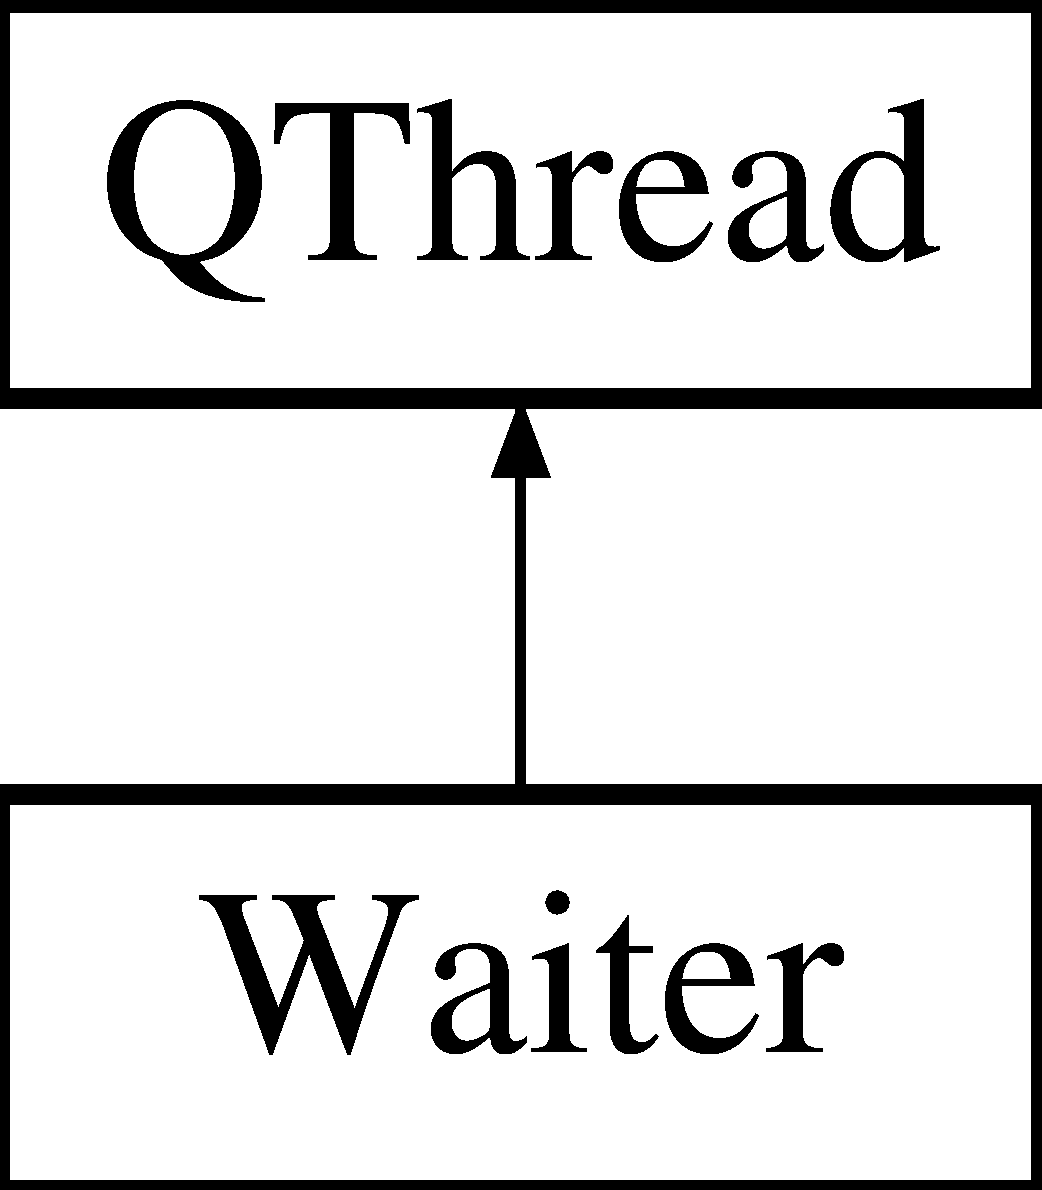
\includegraphics[height=2.000000cm]{classWaiter}
\end{center}
\end{figure}
\subsection*{Public Member Functions}
\begin{DoxyCompactItemize}
\item 
\hyperlink{classWaiter_a8c26bfa810034fca946ad2517442950a}{Waiter} (long msecs)
\item 
void \hyperlink{classWaiter_a313daa52281a1dca00f211e6df2f2676}{run} ()
\end{DoxyCompactItemize}


\subsection{Detailed Description}
Smartphone Brain Scanner 2 License Agreement (M\-I\-T License)

Copyright (c) 2012 Arkadiusz Stopczynski, Jakob Eg Larsen, Carsten Stahlhut, Michael Kai Petersen, Lars Kai Hansen. Technical University of Denmark, \hyperlink{namespaceDTU}{D\-T\-U} Informatics, Cognitive Systems Section. \href{http://code.google.com/p/smartphonebrainscanner2}{\tt http\-://code.\-google.\-com/p/smartphonebrainscanner2}

Permission is hereby granted, free of charge, to any person obtaining a copy of this software and associated documentation files (the \char`\"{}\-Software\char`\"{}), to deal in the Software without restriction, including without limitation the rights to use, copy, modify, merge, publish, distribute, sublicense, and/or sell copies of the Software, and to permit persons to whom the Software is furnished to do so, subject to the following conditions\-:

The above copyright notice and this permission notice shall be included in all copies or substantial portions of the Software.

T\-H\-E S\-O\-F\-T\-W\-A\-R\-E I\-S P\-R\-O\-V\-I\-D\-E\-D \char`\"{}\-A\-S I\-S\char`\"{}, W\-I\-T\-H\-O\-U\-T W\-A\-R\-R\-A\-N\-T\-Y O\-F A\-N\-Y K\-I\-N\-D, E\-X\-P\-R\-E\-S\-S O\-R I\-M\-P\-L\-I\-E\-D, I\-N\-C\-L\-U\-D\-I\-N\-G B\-U\-T N\-O\-T L\-I\-M\-I\-T\-E\-D T\-O T\-H\-E W\-A\-R\-R\-A\-N\-T\-I\-E\-S O\-F M\-E\-R\-C\-H\-A\-N\-T\-A\-B\-I\-L\-I\-T\-Y, F\-I\-T\-N\-E\-S\-S F\-O\-R A P\-A\-R\-T\-I\-C\-U\-L\-A\-R P\-U\-R\-P\-O\-S\-E A\-N\-D N\-O\-N\-I\-N\-F\-R\-I\-N\-G\-E\-M\-E\-N\-T. I\-N N\-O E\-V\-E\-N\-T S\-H\-A\-L\-L T\-H\-E A\-U\-T\-H\-O\-R\-S O\-R C\-O\-P\-Y\-R\-I\-G\-H\-T H\-O\-L\-D\-E\-R\-S B\-E L\-I\-A\-B\-L\-E F\-O\-R A\-N\-Y C\-L\-A\-I\-M, D\-A\-M\-A\-G\-E\-S O\-R O\-T\-H\-E\-R L\-I\-A\-B\-I\-L\-I\-T\-Y, W\-H\-E\-T\-H\-E\-R I\-N A\-N A\-C\-T\-I\-O\-N O\-F C\-O\-N\-T\-R\-A\-C\-T, T\-O\-R\-T O\-R O\-T\-H\-E\-R\-W\-I\-S\-E, A\-R\-I\-S\-I\-N\-G F\-R\-O\-M, O\-U\-T O\-F O\-R I\-N C\-O\-N\-N\-E\-C\-T\-I\-O\-N W\-I\-T\-H T\-H\-E S\-O\-F\-T\-W\-A\-R\-E O\-R T\-H\-E U\-S\-E O\-R O\-T\-H\-E\-R D\-E\-A\-L\-I\-N\-G\-S I\-N T\-H\-E S\-O\-F\-T\-W\-A\-R\-E. 

\subsection{Constructor \& Destructor Documentation}
\hypertarget{classWaiter_a8c26bfa810034fca946ad2517442950a}{\index{Waiter@{Waiter}!Waiter@{Waiter}}
\index{Waiter@{Waiter}!Waiter@{Waiter}}
\subsubsection[{Waiter}]{\setlength{\rightskip}{0pt plus 5cm}Waiter\-::\-Waiter (
\begin{DoxyParamCaption}
\item[{long}]{msecs}
\end{DoxyParamCaption}
)\hspace{0.3cm}{\ttfamily [inline]}}}\label{classWaiter_a8c26bfa810034fca946ad2517442950a}


\subsection{Member Function Documentation}
\hypertarget{classWaiter_a313daa52281a1dca00f211e6df2f2676}{\index{Waiter@{Waiter}!run@{run}}
\index{run@{run}!Waiter@{Waiter}}
\subsubsection[{run}]{\setlength{\rightskip}{0pt plus 5cm}void Waiter\-::run (
\begin{DoxyParamCaption}
{}
\end{DoxyParamCaption}
)\hspace{0.3cm}{\ttfamily [inline]}}}\label{classWaiter_a313daa52281a1dca00f211e6df2f2676}


The documentation for this class was generated from the following file\-:\begin{DoxyCompactItemize}
\item 
/media/philipjhj/\-Data/\-One\-Drive/\-Studie/\-Studenterprogrammør/\-S\-B\-S3/smartphonebrainscanner2-\/core/src/utils/\hyperlink{waiter_8h}{waiter.\-h}\end{DoxyCompactItemize}

\chapter{File Documentation}
\hypertarget{documentation__static_8cpp}{\section{/media/philipjhj/\-Data/\-One\-Drive/\-Studie/\-Studenterprogrammør/\-S\-B\-S3/smartphonebrainscanner2-\/core/src/documentation\-\_\-static.cpp File Reference}
\label{documentation__static_8cpp}\index{/media/philipjhj/\-Data/\-One\-Drive/\-Studie/\-Studenterprogrammør/\-S\-B\-S3/smartphonebrainscanner2-\/core/src/documentation\-\_\-static.\-cpp@{/media/philipjhj/\-Data/\-One\-Drive/\-Studie/\-Studenterprogrammør/\-S\-B\-S3/smartphonebrainscanner2-\/core/src/documentation\-\_\-static.\-cpp}}
}

\hypertarget{dtu__array__2d_8h}{\section{/media/philipjhj/\-Data/\-One\-Drive/\-Studie/\-Studenterprogrammør/\-S\-B\-S3/smartphonebrainscanner2-\/core/src/dtu\-\_\-array\-\_\-2d.h File Reference}
\label{dtu__array__2d_8h}\index{/media/philipjhj/\-Data/\-One\-Drive/\-Studie/\-Studenterprogrammør/\-S\-B\-S3/smartphonebrainscanner2-\/core/src/dtu\-\_\-array\-\_\-2d.\-h@{/media/philipjhj/\-Data/\-One\-Drive/\-Studie/\-Studenterprogrammør/\-S\-B\-S3/smartphonebrainscanner2-\/core/src/dtu\-\_\-array\-\_\-2d.\-h}}
}
{\ttfamily \#include $<$math.\-h$>$}\\*
{\ttfamily \#include \char`\"{}jama125/tnt\-\_\-array2d.\-h\char`\"{}}\\*
{\ttfamily \#include \char`\"{}jama125/tnt\-\_\-array2d\-\_\-utils.\-h\char`\"{}}\\*
{\ttfamily \#include \char`\"{}jama125/jama\-\_\-svd.\-h\char`\"{}}\\*
\subsection*{Classes}
\begin{DoxyCompactItemize}
\item 
class \hyperlink{classDTU_1_1DtuArray2D}{D\-T\-U\-::\-Dtu\-Array2\-D$<$ T $>$}
\end{DoxyCompactItemize}
\subsection*{Namespaces}
\begin{DoxyCompactItemize}
\item 
\hyperlink{namespaceDTU}{D\-T\-U}
\end{DoxyCompactItemize}

\hypertarget{FFTReal_8cpp}{\section{/media/philipjhj/\-Data/\-One\-Drive/\-Studie/\-Studenterprogrammør/\-S\-B\-S3/smartphonebrainscanner2-\/core/src/\-F\-F\-T\-Real.cpp File Reference}
\label{FFTReal_8cpp}\index{/media/philipjhj/\-Data/\-One\-Drive/\-Studie/\-Studenterprogrammør/\-S\-B\-S3/smartphonebrainscanner2-\/core/src/\-F\-F\-T\-Real.\-cpp@{/media/philipjhj/\-Data/\-One\-Drive/\-Studie/\-Studenterprogrammør/\-S\-B\-S3/smartphonebrainscanner2-\/core/src/\-F\-F\-T\-Real.\-cpp}}
}
{\ttfamily \#include \char`\"{}F\-F\-T\-Real.\-h\char`\"{}}\\*
{\ttfamily \#include $<$cassert$>$}\\*
{\ttfamily \#include $<$cmath$>$}\\*

\hypertarget{FFTReal_8h}{\section{/media/philipjhj/\-Data/\-One\-Drive/\-Studie/\-Studenterprogrammør/\-S\-B\-S3/smartphonebrainscanner2-\/core/src/\-F\-F\-T\-Real.h File Reference}
\label{FFTReal_8h}\index{/media/philipjhj/\-Data/\-One\-Drive/\-Studie/\-Studenterprogrammør/\-S\-B\-S3/smartphonebrainscanner2-\/core/src/\-F\-F\-T\-Real.\-h@{/media/philipjhj/\-Data/\-One\-Drive/\-Studie/\-Studenterprogrammør/\-S\-B\-S3/smartphonebrainscanner2-\/core/src/\-F\-F\-T\-Real.\-h}}
}
\subsection*{Classes}
\begin{DoxyCompactItemize}
\item 
class \hyperlink{classFFTReal}{F\-F\-T\-Real}
\end{DoxyCompactItemize}
\subsection*{Macros}
\begin{DoxyCompactItemize}
\item 
\#define \hyperlink{FFTReal_8h_a5386cb625b0754f62becb0eac67f5d46}{F\-F\-T\-Real\-\_\-\-C\-U\-R\-R\-E\-N\-T\-\_\-\-H\-E\-A\-D\-E\-R}
\item 
\#define \hyperlink{FFTReal_8h_a1c01c2bbbc2964e267014f4e3afdb94b}{F\-F\-T\-Real\-\_\-\-H\-E\-A\-D\-E\-R\-\_\-\-I\-N\-C\-L\-U\-D\-E\-D}
\end{DoxyCompactItemize}
\subsection*{Typedefs}
\begin{DoxyCompactItemize}
\item 
typedef double \hyperlink{FFTReal_8h_a98b5402b1616416bbb3e31e90c38ea3f}{flt\-\_\-t}
\end{DoxyCompactItemize}


\subsection{Macro Definition Documentation}
\hypertarget{FFTReal_8h_a5386cb625b0754f62becb0eac67f5d46}{\index{F\-F\-T\-Real.\-h@{F\-F\-T\-Real.\-h}!F\-F\-T\-Real\-\_\-\-C\-U\-R\-R\-E\-N\-T\-\_\-\-H\-E\-A\-D\-E\-R@{F\-F\-T\-Real\-\_\-\-C\-U\-R\-R\-E\-N\-T\-\_\-\-H\-E\-A\-D\-E\-R}}
\index{F\-F\-T\-Real\-\_\-\-C\-U\-R\-R\-E\-N\-T\-\_\-\-H\-E\-A\-D\-E\-R@{F\-F\-T\-Real\-\_\-\-C\-U\-R\-R\-E\-N\-T\-\_\-\-H\-E\-A\-D\-E\-R}!FFTReal.h@{F\-F\-T\-Real.\-h}}
\subsubsection[{F\-F\-T\-Real\-\_\-\-C\-U\-R\-R\-E\-N\-T\-\_\-\-H\-E\-A\-D\-E\-R}]{\setlength{\rightskip}{0pt plus 5cm}\#define F\-F\-T\-Real\-\_\-\-C\-U\-R\-R\-E\-N\-T\-\_\-\-H\-E\-A\-D\-E\-R}}\label{FFTReal_8h_a5386cb625b0754f62becb0eac67f5d46}
\hypertarget{FFTReal_8h_a1c01c2bbbc2964e267014f4e3afdb94b}{\index{F\-F\-T\-Real.\-h@{F\-F\-T\-Real.\-h}!F\-F\-T\-Real\-\_\-\-H\-E\-A\-D\-E\-R\-\_\-\-I\-N\-C\-L\-U\-D\-E\-D@{F\-F\-T\-Real\-\_\-\-H\-E\-A\-D\-E\-R\-\_\-\-I\-N\-C\-L\-U\-D\-E\-D}}
\index{F\-F\-T\-Real\-\_\-\-H\-E\-A\-D\-E\-R\-\_\-\-I\-N\-C\-L\-U\-D\-E\-D@{F\-F\-T\-Real\-\_\-\-H\-E\-A\-D\-E\-R\-\_\-\-I\-N\-C\-L\-U\-D\-E\-D}!FFTReal.h@{F\-F\-T\-Real.\-h}}
\subsubsection[{F\-F\-T\-Real\-\_\-\-H\-E\-A\-D\-E\-R\-\_\-\-I\-N\-C\-L\-U\-D\-E\-D}]{\setlength{\rightskip}{0pt plus 5cm}\#define F\-F\-T\-Real\-\_\-\-H\-E\-A\-D\-E\-R\-\_\-\-I\-N\-C\-L\-U\-D\-E\-D}}\label{FFTReal_8h_a1c01c2bbbc2964e267014f4e3afdb94b}


\subsection{Typedef Documentation}
\hypertarget{FFTReal_8h_a98b5402b1616416bbb3e31e90c38ea3f}{\index{F\-F\-T\-Real.\-h@{F\-F\-T\-Real.\-h}!flt\-\_\-t@{flt\-\_\-t}}
\index{flt\-\_\-t@{flt\-\_\-t}!FFTReal.h@{F\-F\-T\-Real.\-h}}
\subsubsection[{flt\-\_\-t}]{\setlength{\rightskip}{0pt plus 5cm}typedef double {\bf flt\-\_\-t}}}\label{FFTReal_8h_a98b5402b1616416bbb3e31e90c38ea3f}

\hypertarget{sbs2emocapdatareader_8cpp}{\section{/media/philipjhj/\-Data/\-One\-Drive/\-Studie/\-Studenterprogrammør/\-S\-B\-S3/smartphonebrainscanner2-\/core/src/hardware/emocap/sbs2emocapdatareader.cpp File Reference}
\label{sbs2emocapdatareader_8cpp}\index{/media/philipjhj/\-Data/\-One\-Drive/\-Studie/\-Studenterprogrammør/\-S\-B\-S3/smartphonebrainscanner2-\/core/src/hardware/emocap/sbs2emocapdatareader.\-cpp@{/media/philipjhj/\-Data/\-One\-Drive/\-Studie/\-Studenterprogrammør/\-S\-B\-S3/smartphonebrainscanner2-\/core/src/hardware/emocap/sbs2emocapdatareader.\-cpp}}
}
{\ttfamily \#include $<$hardware/emocap/sbs2emocapdatareader.\-h$>$}\\*

\hypertarget{sbs2emocapdatareader_8h}{\section{/media/philipjhj/\-Data/\-One\-Drive/\-Studie/\-Studenterprogrammør/\-S\-B\-S3/smartphonebrainscanner2-\/core/src/hardware/emocap/sbs2emocapdatareader.h File Reference}
\label{sbs2emocapdatareader_8h}\index{/media/philipjhj/\-Data/\-One\-Drive/\-Studie/\-Studenterprogrammør/\-S\-B\-S3/smartphonebrainscanner2-\/core/src/hardware/emocap/sbs2emocapdatareader.\-h@{/media/philipjhj/\-Data/\-One\-Drive/\-Studie/\-Studenterprogrammør/\-S\-B\-S3/smartphonebrainscanner2-\/core/src/hardware/emocap/sbs2emocapdatareader.\-h}}
}
{\ttfamily \#include $<$hardware/sbs2datareader.\-h$>$}\\*
{\ttfamily \#include $<$hardware/emocap/sbs2emocapmounter.\-h$>$}\\*
{\ttfamily \#include $<$hardware/emotiv/sbs2emotivdecryptor.\-h$>$}\\*
{\ttfamily \#include $<$hardware/emocap/sbs2emocappacket.\-h$>$}\\*
\subsection*{Classes}
\begin{DoxyCompactItemize}
\item 
class \hyperlink{classSbs2EmocapDataReader}{Sbs2\-Emocap\-Data\-Reader}
\end{DoxyCompactItemize}

\hypertarget{sbs2emocapmounter_8cpp}{\section{/media/philipjhj/\-Data/\-One\-Drive/\-Studie/\-Studenterprogrammør/\-S\-B\-S3/smartphonebrainscanner2-\/core/src/hardware/emocap/sbs2emocapmounter.cpp File Reference}
\label{sbs2emocapmounter_8cpp}\index{/media/philipjhj/\-Data/\-One\-Drive/\-Studie/\-Studenterprogrammør/\-S\-B\-S3/smartphonebrainscanner2-\/core/src/hardware/emocap/sbs2emocapmounter.\-cpp@{/media/philipjhj/\-Data/\-One\-Drive/\-Studie/\-Studenterprogrammør/\-S\-B\-S3/smartphonebrainscanner2-\/core/src/hardware/emocap/sbs2emocapmounter.\-cpp}}
}
{\ttfamily \#include $<$hardware/emocap/sbs2emocapmounter.\-h$>$}\\*

\hypertarget{sbs2emocapmounter_8h}{\section{/media/philipjhj/\-Data/\-One\-Drive/\-Studie/\-Studenterprogrammør/\-S\-B\-S3/smartphonebrainscanner2-\/core/src/hardware/emocap/sbs2emocapmounter.h File Reference}
\label{sbs2emocapmounter_8h}\index{/media/philipjhj/\-Data/\-One\-Drive/\-Studie/\-Studenterprogrammør/\-S\-B\-S3/smartphonebrainscanner2-\/core/src/hardware/emocap/sbs2emocapmounter.\-h@{/media/philipjhj/\-Data/\-One\-Drive/\-Studie/\-Studenterprogrammør/\-S\-B\-S3/smartphonebrainscanner2-\/core/src/hardware/emocap/sbs2emocapmounter.\-h}}
}
{\ttfamily \#include $<$hardware/sbs2hardwaremounter.\-h$>$}\\*
\subsection*{Classes}
\begin{DoxyCompactItemize}
\item 
class \hyperlink{classSbs2EmocapMounter}{Sbs2\-Emocap\-Mounter}
\end{DoxyCompactItemize}

\hypertarget{sbs2emocappacket_8cpp}{\section{/media/philipjhj/\-Data/\-One\-Drive/\-Studie/\-Studenterprogrammør/\-S\-B\-S3/smartphonebrainscanner2-\/core/src/hardware/emocap/sbs2emocappacket.cpp File Reference}
\label{sbs2emocappacket_8cpp}\index{/media/philipjhj/\-Data/\-One\-Drive/\-Studie/\-Studenterprogrammør/\-S\-B\-S3/smartphonebrainscanner2-\/core/src/hardware/emocap/sbs2emocappacket.\-cpp@{/media/philipjhj/\-Data/\-One\-Drive/\-Studie/\-Studenterprogrammør/\-S\-B\-S3/smartphonebrainscanner2-\/core/src/hardware/emocap/sbs2emocappacket.\-cpp}}
}
{\ttfamily \#include $<$hardware/emocap/sbs2emocappacket.\-h$>$}\\*

\hypertarget{sbs2emocappacket_8h}{\section{/media/philipjhj/\-Data/\-One\-Drive/\-Studie/\-Studenterprogrammør/\-S\-B\-S3/smartphonebrainscanner2-\/core/src/hardware/emocap/sbs2emocappacket.h File Reference}
\label{sbs2emocappacket_8h}\index{/media/philipjhj/\-Data/\-One\-Drive/\-Studie/\-Studenterprogrammør/\-S\-B\-S3/smartphonebrainscanner2-\/core/src/hardware/emocap/sbs2emocappacket.\-h@{/media/philipjhj/\-Data/\-One\-Drive/\-Studie/\-Studenterprogrammør/\-S\-B\-S3/smartphonebrainscanner2-\/core/src/hardware/emocap/sbs2emocappacket.\-h}}
}
{\ttfamily \#include $<$hardware/sbs2packet.\-h$>$}\\*
\subsection*{Classes}
\begin{DoxyCompactItemize}
\item 
class \hyperlink{classSbs2EmocapPacket}{Sbs2\-Emocap\-Packet}
\end{DoxyCompactItemize}

\hypertarget{sbs2emocap28datareader_8cpp}{\section{/media/philipjhj/\-Data/\-One\-Drive/\-Studie/\-Studenterprogrammør/\-S\-B\-S3/smartphonebrainscanner2-\/core/src/hardware/emocap28/sbs2emocap28datareader.cpp File Reference}
\label{sbs2emocap28datareader_8cpp}\index{/media/philipjhj/\-Data/\-One\-Drive/\-Studie/\-Studenterprogrammør/\-S\-B\-S3/smartphonebrainscanner2-\/core/src/hardware/emocap28/sbs2emocap28datareader.\-cpp@{/media/philipjhj/\-Data/\-One\-Drive/\-Studie/\-Studenterprogrammør/\-S\-B\-S3/smartphonebrainscanner2-\/core/src/hardware/emocap28/sbs2emocap28datareader.\-cpp}}
}
{\ttfamily \#include $<$hardware/emocap28/sbs2emocap28datareader.\-h$>$}\\*
\subsection*{Functions}
\begin{DoxyCompactItemize}
\item 
int \hyperlink{sbs2emocap28datareader_8cpp_a955be2809aad4f747bbe342128745fb0}{mod} (int x, int m)
\item 
bool \hyperlink{sbs2emocap28datareader_8cpp_a93ed27c429bf643739a4ab996deffff2}{less\-Than} (const Q\-Vector$<$ double $>$ \&s1, const Q\-Vector$<$ double $>$ \&s2)
\end{DoxyCompactItemize}


\subsection{Function Documentation}
\hypertarget{sbs2emocap28datareader_8cpp_a93ed27c429bf643739a4ab996deffff2}{\index{sbs2emocap28datareader.\-cpp@{sbs2emocap28datareader.\-cpp}!less\-Than@{less\-Than}}
\index{less\-Than@{less\-Than}!sbs2emocap28datareader.cpp@{sbs2emocap28datareader.\-cpp}}
\subsubsection[{less\-Than}]{\setlength{\rightskip}{0pt plus 5cm}bool less\-Than (
\begin{DoxyParamCaption}
\item[{const Q\-Vector$<$ double $>$ \&}]{s1, }
\item[{const Q\-Vector$<$ double $>$ \&}]{s2}
\end{DoxyParamCaption}
)}}\label{sbs2emocap28datareader_8cpp_a93ed27c429bf643739a4ab996deffff2}
\hypertarget{sbs2emocap28datareader_8cpp_a955be2809aad4f747bbe342128745fb0}{\index{sbs2emocap28datareader.\-cpp@{sbs2emocap28datareader.\-cpp}!mod@{mod}}
\index{mod@{mod}!sbs2emocap28datareader.cpp@{sbs2emocap28datareader.\-cpp}}
\subsubsection[{mod}]{\setlength{\rightskip}{0pt plus 5cm}int mod (
\begin{DoxyParamCaption}
\item[{int}]{x, }
\item[{int}]{m}
\end{DoxyParamCaption}
)}}\label{sbs2emocap28datareader_8cpp_a955be2809aad4f747bbe342128745fb0}

\hypertarget{sbs2emocap28datareader_8h}{\section{/media/philipjhj/\-Data/\-One\-Drive/\-Studie/\-Studenterprogrammør/\-S\-B\-S3/smartphonebrainscanner2-\/core/src/hardware/emocap28/sbs2emocap28datareader.h File Reference}
\label{sbs2emocap28datareader_8h}\index{/media/philipjhj/\-Data/\-One\-Drive/\-Studie/\-Studenterprogrammør/\-S\-B\-S3/smartphonebrainscanner2-\/core/src/hardware/emocap28/sbs2emocap28datareader.\-h@{/media/philipjhj/\-Data/\-One\-Drive/\-Studie/\-Studenterprogrammør/\-S\-B\-S3/smartphonebrainscanner2-\/core/src/hardware/emocap28/sbs2emocap28datareader.\-h}}
}
{\ttfamily \#include $<$hardware/sbs2datareader.\-h$>$}\\*
{\ttfamily \#include $<$hardware/emocap28/sbs2emocap28mounter.\-h$>$}\\*
{\ttfamily \#include $<$hardware/emotiv/sbs2emotivdecryptor.\-h$>$}\\*
{\ttfamily \#include $<$hardware/emocap28/sbs2emocap28packet.\-h$>$}\\*
\subsection*{Classes}
\begin{DoxyCompactItemize}
\item 
class \hyperlink{classSbs2Emocap28DataContainer}{Sbs2\-Emocap28\-Data\-Container}
\item 
class \hyperlink{classSbs2Emocap28DataReader}{Sbs2\-Emocap28\-Data\-Reader}
\end{DoxyCompactItemize}

\hypertarget{sbs2emocap28mounter_8cpp}{\section{/media/philipjhj/\-Data/\-One\-Drive/\-Studie/\-Studenterprogrammør/\-S\-B\-S3/smartphonebrainscanner2-\/core/src/hardware/emocap28/sbs2emocap28mounter.cpp File Reference}
\label{sbs2emocap28mounter_8cpp}\index{/media/philipjhj/\-Data/\-One\-Drive/\-Studie/\-Studenterprogrammør/\-S\-B\-S3/smartphonebrainscanner2-\/core/src/hardware/emocap28/sbs2emocap28mounter.\-cpp@{/media/philipjhj/\-Data/\-One\-Drive/\-Studie/\-Studenterprogrammør/\-S\-B\-S3/smartphonebrainscanner2-\/core/src/hardware/emocap28/sbs2emocap28mounter.\-cpp}}
}
{\ttfamily \#include $<$hardware/emocap28/sbs2emocap28mounter.\-h$>$}\\*

\hypertarget{sbs2emocap28mounter_8h}{\section{/media/philipjhj/\-Data/\-One\-Drive/\-Studie/\-Studenterprogrammør/\-S\-B\-S3/smartphonebrainscanner2-\/core/src/hardware/emocap28/sbs2emocap28mounter.h File Reference}
\label{sbs2emocap28mounter_8h}\index{/media/philipjhj/\-Data/\-One\-Drive/\-Studie/\-Studenterprogrammør/\-S\-B\-S3/smartphonebrainscanner2-\/core/src/hardware/emocap28/sbs2emocap28mounter.\-h@{/media/philipjhj/\-Data/\-One\-Drive/\-Studie/\-Studenterprogrammør/\-S\-B\-S3/smartphonebrainscanner2-\/core/src/hardware/emocap28/sbs2emocap28mounter.\-h}}
}
{\ttfamily \#include $<$hardware/sbs2hardwaremounter.\-h$>$}\\*
\subsection*{Classes}
\begin{DoxyCompactItemize}
\item 
class \hyperlink{classSbs2Emocap28Mounter}{Sbs2\-Emocap28\-Mounter}
\end{DoxyCompactItemize}

\hypertarget{sbs2emocap28packet_8cpp}{\section{/media/philipjhj/\-Data/\-One\-Drive/\-Studie/\-Studenterprogrammør/\-S\-B\-S3/smartphonebrainscanner2-\/core/src/hardware/emocap28/sbs2emocap28packet.cpp File Reference}
\label{sbs2emocap28packet_8cpp}\index{/media/philipjhj/\-Data/\-One\-Drive/\-Studie/\-Studenterprogrammør/\-S\-B\-S3/smartphonebrainscanner2-\/core/src/hardware/emocap28/sbs2emocap28packet.\-cpp@{/media/philipjhj/\-Data/\-One\-Drive/\-Studie/\-Studenterprogrammør/\-S\-B\-S3/smartphonebrainscanner2-\/core/src/hardware/emocap28/sbs2emocap28packet.\-cpp}}
}
{\ttfamily \#include $<$hardware/emocap28/sbs2emocap28packet.\-h$>$}\\*

\hypertarget{sbs2emocap28packet_8h}{\section{/media/philipjhj/\-Data/\-One\-Drive/\-Studie/\-Studenterprogrammør/\-S\-B\-S3/smartphonebrainscanner2-\/core/src/hardware/emocap28/sbs2emocap28packet.h File Reference}
\label{sbs2emocap28packet_8h}\index{/media/philipjhj/\-Data/\-One\-Drive/\-Studie/\-Studenterprogrammør/\-S\-B\-S3/smartphonebrainscanner2-\/core/src/hardware/emocap28/sbs2emocap28packet.\-h@{/media/philipjhj/\-Data/\-One\-Drive/\-Studie/\-Studenterprogrammør/\-S\-B\-S3/smartphonebrainscanner2-\/core/src/hardware/emocap28/sbs2emocap28packet.\-h}}
}
{\ttfamily \#include $<$hardware/sbs2packet.\-h$>$}\\*
\subsection*{Classes}
\begin{DoxyCompactItemize}
\item 
class \hyperlink{classSbs2Emocap28Packet}{Sbs2\-Emocap28\-Packet}
\end{DoxyCompactItemize}

\hypertarget{sbs2emotivdatareader_8cpp}{\section{/media/philipjhj/\-Data/\-One\-Drive/\-Studie/\-Studenterprogrammør/\-S\-B\-S3/smartphonebrainscanner2-\/core/src/hardware/emotiv/sbs2emotivdatareader.cpp File Reference}
\label{sbs2emotivdatareader_8cpp}\index{/media/philipjhj/\-Data/\-One\-Drive/\-Studie/\-Studenterprogrammør/\-S\-B\-S3/smartphonebrainscanner2-\/core/src/hardware/emotiv/sbs2emotivdatareader.\-cpp@{/media/philipjhj/\-Data/\-One\-Drive/\-Studie/\-Studenterprogrammør/\-S\-B\-S3/smartphonebrainscanner2-\/core/src/hardware/emotiv/sbs2emotivdatareader.\-cpp}}
}
{\ttfamily \#include $<$hardware/emotiv/sbs2emotivdatareader.\-h$>$}\\*

\hypertarget{sbs2emotivdatareader_8h}{\section{/media/philipjhj/\-Data/\-One\-Drive/\-Studie/\-Studenterprogrammør/\-S\-B\-S3/smartphonebrainscanner2-\/core/src/hardware/emotiv/sbs2emotivdatareader.h File Reference}
\label{sbs2emotivdatareader_8h}\index{/media/philipjhj/\-Data/\-One\-Drive/\-Studie/\-Studenterprogrammør/\-S\-B\-S3/smartphonebrainscanner2-\/core/src/hardware/emotiv/sbs2emotivdatareader.\-h@{/media/philipjhj/\-Data/\-One\-Drive/\-Studie/\-Studenterprogrammør/\-S\-B\-S3/smartphonebrainscanner2-\/core/src/hardware/emotiv/sbs2emotivdatareader.\-h}}
}
{\ttfamily \#include $<$hardware/sbs2datareader.\-h$>$}\\*
{\ttfamily \#include $<$hardware/emotiv/sbs2emotivmounter.\-h$>$}\\*
{\ttfamily \#include $<$hardware/emotiv/sbs2emotivdecryptor.\-h$>$}\\*
{\ttfamily \#include $<$hardware/emotiv/sbs2emotivpacket.\-h$>$}\\*
\subsection*{Classes}
\begin{DoxyCompactItemize}
\item 
class \hyperlink{classSbs2EmotivDataReader}{Sbs2\-Emotiv\-Data\-Reader}
\end{DoxyCompactItemize}

\hypertarget{sbs2emotivdecryptor_8h}{\section{/media/philipjhj/\-Data/\-One\-Drive/\-Studie/\-Studenterprogrammør/\-S\-B\-S3/smartphonebrainscanner2-\/core/src/hardware/emotiv/sbs2emotivdecryptor.h File Reference}
\label{sbs2emotivdecryptor_8h}\index{/media/philipjhj/\-Data/\-One\-Drive/\-Studie/\-Studenterprogrammør/\-S\-B\-S3/smartphonebrainscanner2-\/core/src/hardware/emotiv/sbs2emotivdecryptor.\-h@{/media/philipjhj/\-Data/\-One\-Drive/\-Studie/\-Studenterprogrammør/\-S\-B\-S3/smartphonebrainscanner2-\/core/src/hardware/emotiv/sbs2emotivdecryptor.\-h}}
}
{\ttfamily \#include $<$Q\-Object$>$}\\*
{\ttfamily \#include $<$utils/\-Rijndael.\-h$>$}\\*
{\ttfamily \#include $<$Q\-Debug$>$}\\*
\subsection*{Classes}
\begin{DoxyCompactItemize}
\item 
class \hyperlink{classSbs2EmotivDecryptor}{Sbs2\-Emotiv\-Decryptor}
\end{DoxyCompactItemize}

\hypertarget{sbs2emotivdecryptor__dummy_8cpp}{\section{/media/philipjhj/\-Data/\-One\-Drive/\-Studie/\-Studenterprogrammør/\-S\-B\-S3/smartphonebrainscanner2-\/core/src/hardware/emotiv/sbs2emotivdecryptor\-\_\-dummy.cpp File Reference}
\label{sbs2emotivdecryptor__dummy_8cpp}\index{/media/philipjhj/\-Data/\-One\-Drive/\-Studie/\-Studenterprogrammør/\-S\-B\-S3/smartphonebrainscanner2-\/core/src/hardware/emotiv/sbs2emotivdecryptor\-\_\-dummy.\-cpp@{/media/philipjhj/\-Data/\-One\-Drive/\-Studie/\-Studenterprogrammør/\-S\-B\-S3/smartphonebrainscanner2-\/core/src/hardware/emotiv/sbs2emotivdecryptor\-\_\-dummy.\-cpp}}
}
{\ttfamily \#include \char`\"{}sbs2emotivdecryptor.\-h\char`\"{}}\\*

\hypertarget{sbs2emotivmounter_8cpp}{\section{/media/philipjhj/\-Data/\-One\-Drive/\-Studie/\-Studenterprogrammør/\-S\-B\-S3/smartphonebrainscanner2-\/core/src/hardware/emotiv/sbs2emotivmounter.cpp File Reference}
\label{sbs2emotivmounter_8cpp}\index{/media/philipjhj/\-Data/\-One\-Drive/\-Studie/\-Studenterprogrammør/\-S\-B\-S3/smartphonebrainscanner2-\/core/src/hardware/emotiv/sbs2emotivmounter.\-cpp@{/media/philipjhj/\-Data/\-One\-Drive/\-Studie/\-Studenterprogrammør/\-S\-B\-S3/smartphonebrainscanner2-\/core/src/hardware/emotiv/sbs2emotivmounter.\-cpp}}
}
{\ttfamily \#include $<$hardware/emotiv/sbs2emotivmounter.\-h$>$}\\*
{\ttfamily \#include \char`\"{}Q\-File\char`\"{}}\\*

\hypertarget{sbs2emotivmounter_8h}{\section{/media/philipjhj/\-Data/\-One\-Drive/\-Studie/\-Studenterprogrammør/\-S\-B\-S3/smartphonebrainscanner2-\/core/src/hardware/emotiv/sbs2emotivmounter.h File Reference}
\label{sbs2emotivmounter_8h}\index{/media/philipjhj/\-Data/\-One\-Drive/\-Studie/\-Studenterprogrammør/\-S\-B\-S3/smartphonebrainscanner2-\/core/src/hardware/emotiv/sbs2emotivmounter.\-h@{/media/philipjhj/\-Data/\-One\-Drive/\-Studie/\-Studenterprogrammør/\-S\-B\-S3/smartphonebrainscanner2-\/core/src/hardware/emotiv/sbs2emotivmounter.\-h}}
}
{\ttfamily \#include $<$hardware/sbs2hardwaremounter.\-h$>$}\\*
\subsection*{Classes}
\begin{DoxyCompactItemize}
\item 
class \hyperlink{classSbs2EmotivMounter}{Sbs2\-Emotiv\-Mounter}
\end{DoxyCompactItemize}

\hypertarget{sbs2emotivpacket_8cpp}{\section{/media/philipjhj/\-Data/\-One\-Drive/\-Studie/\-Studenterprogrammør/\-S\-B\-S3/smartphonebrainscanner2-\/core/src/hardware/emotiv/sbs2emotivpacket.cpp File Reference}
\label{sbs2emotivpacket_8cpp}\index{/media/philipjhj/\-Data/\-One\-Drive/\-Studie/\-Studenterprogrammør/\-S\-B\-S3/smartphonebrainscanner2-\/core/src/hardware/emotiv/sbs2emotivpacket.\-cpp@{/media/philipjhj/\-Data/\-One\-Drive/\-Studie/\-Studenterprogrammør/\-S\-B\-S3/smartphonebrainscanner2-\/core/src/hardware/emotiv/sbs2emotivpacket.\-cpp}}
}
{\ttfamily \#include $<$hardware/emotiv/sbs2emotivpacket.\-h$>$}\\*

\hypertarget{sbs2emotivpacket_8h}{\section{/media/philipjhj/\-Data/\-One\-Drive/\-Studie/\-Studenterprogrammør/\-S\-B\-S3/smartphonebrainscanner2-\/core/src/hardware/emotiv/sbs2emotivpacket.h File Reference}
\label{sbs2emotivpacket_8h}\index{/media/philipjhj/\-Data/\-One\-Drive/\-Studie/\-Studenterprogrammør/\-S\-B\-S3/smartphonebrainscanner2-\/core/src/hardware/emotiv/sbs2emotivpacket.\-h@{/media/philipjhj/\-Data/\-One\-Drive/\-Studie/\-Studenterprogrammør/\-S\-B\-S3/smartphonebrainscanner2-\/core/src/hardware/emotiv/sbs2emotivpacket.\-h}}
}
{\ttfamily \#include $<$hardware/sbs2packet.\-h$>$}\\*
\subsection*{Classes}
\begin{DoxyCompactItemize}
\item 
class \hyperlink{classSbs2EmotivPacket}{Sbs2\-Emotiv\-Packet}
\end{DoxyCompactItemize}

\hypertarget{sbs2fakedatareader_8cpp}{\section{/media/philipjhj/\-Data/\-One\-Drive/\-Studie/\-Studenterprogrammør/\-S\-B\-S3/smartphonebrainscanner2-\/core/src/hardware/fake/sbs2fakedatareader.cpp File Reference}
\label{sbs2fakedatareader_8cpp}\index{/media/philipjhj/\-Data/\-One\-Drive/\-Studie/\-Studenterprogrammør/\-S\-B\-S3/smartphonebrainscanner2-\/core/src/hardware/fake/sbs2fakedatareader.\-cpp@{/media/philipjhj/\-Data/\-One\-Drive/\-Studie/\-Studenterprogrammør/\-S\-B\-S3/smartphonebrainscanner2-\/core/src/hardware/fake/sbs2fakedatareader.\-cpp}}
}
{\ttfamily \#include \char`\"{}sbs2fakedatareader.\-h\char`\"{}}\\*
{\ttfamily \#include $<$Qt\-Core$>$}\\*

\hypertarget{sbs2fakedatareader_8h}{\section{/media/philipjhj/\-Data/\-One\-Drive/\-Studie/\-Studenterprogrammør/\-S\-B\-S3/smartphonebrainscanner2-\/core/src/hardware/fake/sbs2fakedatareader.h File Reference}
\label{sbs2fakedatareader_8h}\index{/media/philipjhj/\-Data/\-One\-Drive/\-Studie/\-Studenterprogrammør/\-S\-B\-S3/smartphonebrainscanner2-\/core/src/hardware/fake/sbs2fakedatareader.\-h@{/media/philipjhj/\-Data/\-One\-Drive/\-Studie/\-Studenterprogrammør/\-S\-B\-S3/smartphonebrainscanner2-\/core/src/hardware/fake/sbs2fakedatareader.\-h}}
}
{\ttfamily \#include $<$hardware/sbs2datareader.\-h$>$}\\*
{\ttfamily \#include $<$hardware/fake/sbs2fakepacket.\-h$>$}\\*
\subsection*{Classes}
\begin{DoxyCompactItemize}
\item 
class \hyperlink{classSbs2FakeDataReader}{Sbs2\-Fake\-Data\-Reader}
\end{DoxyCompactItemize}

\hypertarget{sbs2fakepacket_8cpp}{\section{/media/philipjhj/\-Data/\-One\-Drive/\-Studie/\-Studenterprogrammør/\-S\-B\-S3/smartphonebrainscanner2-\/core/src/hardware/fake/sbs2fakepacket.cpp File Reference}
\label{sbs2fakepacket_8cpp}\index{/media/philipjhj/\-Data/\-One\-Drive/\-Studie/\-Studenterprogrammør/\-S\-B\-S3/smartphonebrainscanner2-\/core/src/hardware/fake/sbs2fakepacket.\-cpp@{/media/philipjhj/\-Data/\-One\-Drive/\-Studie/\-Studenterprogrammør/\-S\-B\-S3/smartphonebrainscanner2-\/core/src/hardware/fake/sbs2fakepacket.\-cpp}}
}
{\ttfamily \#include \char`\"{}sbs2fakepacket.\-h\char`\"{}}\\*

\hypertarget{sbs2fakepacket_8h}{\section{/media/philipjhj/\-Data/\-One\-Drive/\-Studie/\-Studenterprogrammør/\-S\-B\-S3/smartphonebrainscanner2-\/core/src/hardware/fake/sbs2fakepacket.h File Reference}
\label{sbs2fakepacket_8h}\index{/media/philipjhj/\-Data/\-One\-Drive/\-Studie/\-Studenterprogrammør/\-S\-B\-S3/smartphonebrainscanner2-\/core/src/hardware/fake/sbs2fakepacket.\-h@{/media/philipjhj/\-Data/\-One\-Drive/\-Studie/\-Studenterprogrammør/\-S\-B\-S3/smartphonebrainscanner2-\/core/src/hardware/fake/sbs2fakepacket.\-h}}
}
{\ttfamily \#include $<$hardware/sbs2packet.\-h$>$}\\*
\subsection*{Classes}
\begin{DoxyCompactItemize}
\item 
class \hyperlink{classSbs2FakePacket}{Sbs2\-Fake\-Packet}
\end{DoxyCompactItemize}

\hypertarget{sbs2datareader_8cpp}{\section{/media/philipjhj/\-Data/\-One\-Drive/\-Studie/\-Studenterprogrammør/\-S\-B\-S3/smartphonebrainscanner2-\/core/src/hardware/sbs2datareader.cpp File Reference}
\label{sbs2datareader_8cpp}\index{/media/philipjhj/\-Data/\-One\-Drive/\-Studie/\-Studenterprogrammør/\-S\-B\-S3/smartphonebrainscanner2-\/core/src/hardware/sbs2datareader.\-cpp@{/media/philipjhj/\-Data/\-One\-Drive/\-Studie/\-Studenterprogrammør/\-S\-B\-S3/smartphonebrainscanner2-\/core/src/hardware/sbs2datareader.\-cpp}}
}
{\ttfamily \#include \char`\"{}sbs2datareader.\-h\char`\"{}}\\*

\hypertarget{sbs2datareader_8h}{\section{/media/philipjhj/\-Data/\-One\-Drive/\-Studie/\-Studenterprogrammør/\-S\-B\-S3/smartphonebrainscanner2-\/core/src/hardware/sbs2datareader.h File Reference}
\label{sbs2datareader_8h}\index{/media/philipjhj/\-Data/\-One\-Drive/\-Studie/\-Studenterprogrammør/\-S\-B\-S3/smartphonebrainscanner2-\/core/src/hardware/sbs2datareader.\-h@{/media/philipjhj/\-Data/\-One\-Drive/\-Studie/\-Studenterprogrammør/\-S\-B\-S3/smartphonebrainscanner2-\/core/src/hardware/sbs2datareader.\-h}}
}
{\ttfamily \#include $<$Q\-Object$>$}\\*
{\ttfamily \#include $<$fstream$>$}\\*
{\ttfamily \#include $<$sbs2callback.\-h$>$}\\*
{\ttfamily \#include $<$sbs2networkhandler.\-h$>$}\\*
\subsection*{Classes}
\begin{DoxyCompactItemize}
\item 
class \hyperlink{classSbs2DataReader}{Sbs2\-Data\-Reader}
\end{DoxyCompactItemize}

\hypertarget{sbs2hardwaremounter_8cpp}{\section{/media/philipjhj/\-Data/\-One\-Drive/\-Studie/\-Studenterprogrammør/\-S\-B\-S3/smartphonebrainscanner2-\/core/src/hardware/sbs2hardwaremounter.cpp File Reference}
\label{sbs2hardwaremounter_8cpp}\index{/media/philipjhj/\-Data/\-One\-Drive/\-Studie/\-Studenterprogrammør/\-S\-B\-S3/smartphonebrainscanner2-\/core/src/hardware/sbs2hardwaremounter.\-cpp@{/media/philipjhj/\-Data/\-One\-Drive/\-Studie/\-Studenterprogrammør/\-S\-B\-S3/smartphonebrainscanner2-\/core/src/hardware/sbs2hardwaremounter.\-cpp}}
}
{\ttfamily \#include $<$hardware/sbs2hardwaremounter.\-h$>$}\\*

\hypertarget{sbs2hardwaremounter_8h}{\section{/media/philipjhj/\-Data/\-One\-Drive/\-Studie/\-Studenterprogrammør/\-S\-B\-S3/smartphonebrainscanner2-\/core/src/hardware/sbs2hardwaremounter.h File Reference}
\label{sbs2hardwaremounter_8h}\index{/media/philipjhj/\-Data/\-One\-Drive/\-Studie/\-Studenterprogrammør/\-S\-B\-S3/smartphonebrainscanner2-\/core/src/hardware/sbs2hardwaremounter.\-h@{/media/philipjhj/\-Data/\-One\-Drive/\-Studie/\-Studenterprogrammør/\-S\-B\-S3/smartphonebrainscanner2-\/core/src/hardware/sbs2hardwaremounter.\-h}}
}
{\ttfamily \#include $<$Q\-Object$>$}\\*
{\ttfamily \#include $<$Q\-Timer$>$}\\*
{\ttfamily \#include $<$Qt\-Core$>$}\\*
{\ttfamily \#include $<$sbs2common.\-h$>$}\\*
{\ttfamily \#include $<$utils/waiter.\-h$>$}\\*
{\ttfamily \#include $<$Q\-String$>$}\\*
\subsection*{Classes}
\begin{DoxyCompactItemize}
\item 
class \hyperlink{classSbs2HardwareMounter}{Sbs2\-Hardware\-Mounter}
\end{DoxyCompactItemize}

\hypertarget{sbs2packet_8cpp}{\section{/media/philipjhj/\-Data/\-One\-Drive/\-Studie/\-Studenterprogrammør/\-S\-B\-S3/smartphonebrainscanner2-\/core/src/hardware/sbs2packet.cpp File Reference}
\label{sbs2packet_8cpp}\index{/media/philipjhj/\-Data/\-One\-Drive/\-Studie/\-Studenterprogrammør/\-S\-B\-S3/smartphonebrainscanner2-\/core/src/hardware/sbs2packet.\-cpp@{/media/philipjhj/\-Data/\-One\-Drive/\-Studie/\-Studenterprogrammør/\-S\-B\-S3/smartphonebrainscanner2-\/core/src/hardware/sbs2packet.\-cpp}}
}
{\ttfamily \#include \char`\"{}sbs2packet.\-h\char`\"{}}\\*

\hypertarget{sbs2packet_8h}{\section{/media/philipjhj/\-Data/\-One\-Drive/\-Studie/\-Studenterprogrammør/\-S\-B\-S3/smartphonebrainscanner2-\/core/src/hardware/sbs2packet.h File Reference}
\label{sbs2packet_8h}\index{/media/philipjhj/\-Data/\-One\-Drive/\-Studie/\-Studenterprogrammør/\-S\-B\-S3/smartphonebrainscanner2-\/core/src/hardware/sbs2packet.\-h@{/media/philipjhj/\-Data/\-One\-Drive/\-Studie/\-Studenterprogrammør/\-S\-B\-S3/smartphonebrainscanner2-\/core/src/hardware/sbs2packet.\-h}}
}
{\ttfamily \#include $<$Q\-Object$>$}\\*
{\ttfamily \#include $<$Q\-Map$>$}\\*
{\ttfamily \#include $<$sbs2common.\-h$>$}\\*
\subsection*{Classes}
\begin{DoxyCompactItemize}
\item 
class \hyperlink{classSbs2Packet}{Sbs2\-Packet}
\end{DoxyCompactItemize}

\hypertarget{jama__cholesky_8h}{\section{/media/philipjhj/\-Data/\-One\-Drive/\-Studie/\-Studenterprogrammør/\-S\-B\-S3/smartphonebrainscanner2-\/core/src/jama125/jama\-\_\-cholesky.h File Reference}
\label{jama__cholesky_8h}\index{/media/philipjhj/\-Data/\-One\-Drive/\-Studie/\-Studenterprogrammør/\-S\-B\-S3/smartphonebrainscanner2-\/core/src/jama125/jama\-\_\-cholesky.\-h@{/media/philipjhj/\-Data/\-One\-Drive/\-Studie/\-Studenterprogrammør/\-S\-B\-S3/smartphonebrainscanner2-\/core/src/jama125/jama\-\_\-cholesky.\-h}}
}
{\ttfamily \#include \char`\"{}math.\-h\char`\"{}}\\*
\subsection*{Classes}
\begin{DoxyCompactItemize}
\item 
class \hyperlink{classJAMA_1_1Cholesky}{J\-A\-M\-A\-::\-Cholesky$<$ Real $>$}
\end{DoxyCompactItemize}
\subsection*{Namespaces}
\begin{DoxyCompactItemize}
\item 
\hyperlink{namespaceJAMA}{J\-A\-M\-A}
\end{DoxyCompactItemize}

\hypertarget{jama__eig_8h}{\section{/media/philipjhj/\-Data/\-One\-Drive/\-Studie/\-Studenterprogrammør/\-S\-B\-S3/smartphonebrainscanner2-\/core/src/jama125/jama\-\_\-eig.h File Reference}
\label{jama__eig_8h}\index{/media/philipjhj/\-Data/\-One\-Drive/\-Studie/\-Studenterprogrammør/\-S\-B\-S3/smartphonebrainscanner2-\/core/src/jama125/jama\-\_\-eig.\-h@{/media/philipjhj/\-Data/\-One\-Drive/\-Studie/\-Studenterprogrammør/\-S\-B\-S3/smartphonebrainscanner2-\/core/src/jama125/jama\-\_\-eig.\-h}}
}
{\ttfamily \#include \char`\"{}tnt\-\_\-array1d.\-h\char`\"{}}\\*
{\ttfamily \#include \char`\"{}tnt\-\_\-array2d.\-h\char`\"{}}\\*
{\ttfamily \#include \char`\"{}tnt\-\_\-math\-\_\-utils.\-h\char`\"{}}\\*
{\ttfamily \#include $<$algorithm$>$}\\*
{\ttfamily \#include $<$cmath$>$}\\*
\subsection*{Classes}
\begin{DoxyCompactItemize}
\item 
class \hyperlink{classJAMA_1_1Eigenvalue}{J\-A\-M\-A\-::\-Eigenvalue$<$ Real $>$}
\end{DoxyCompactItemize}
\subsection*{Namespaces}
\begin{DoxyCompactItemize}
\item 
\hyperlink{namespaceJAMA}{J\-A\-M\-A}
\end{DoxyCompactItemize}

\hypertarget{jama__lu_8h}{\section{/media/philipjhj/\-Data/\-One\-Drive/\-Studie/\-Studenterprogrammør/\-S\-B\-S3/smartphonebrainscanner2-\/core/src/jama125/jama\-\_\-lu.h File Reference}
\label{jama__lu_8h}\index{/media/philipjhj/\-Data/\-One\-Drive/\-Studie/\-Studenterprogrammør/\-S\-B\-S3/smartphonebrainscanner2-\/core/src/jama125/jama\-\_\-lu.\-h@{/media/philipjhj/\-Data/\-One\-Drive/\-Studie/\-Studenterprogrammør/\-S\-B\-S3/smartphonebrainscanner2-\/core/src/jama125/jama\-\_\-lu.\-h}}
}
{\ttfamily \#include \char`\"{}tnt.\-h\char`\"{}}\\*
{\ttfamily \#include $<$algorithm$>$}\\*
\subsection*{Classes}
\begin{DoxyCompactItemize}
\item 
class \hyperlink{classJAMA_1_1LU}{J\-A\-M\-A\-::\-L\-U$<$ Real $>$}
\end{DoxyCompactItemize}
\subsection*{Namespaces}
\begin{DoxyCompactItemize}
\item 
\hyperlink{namespaceJAMA}{J\-A\-M\-A}
\end{DoxyCompactItemize}

\hypertarget{jama__qr_8h}{\section{/media/philipjhj/\-Data/\-One\-Drive/\-Studie/\-Studenterprogrammør/\-S\-B\-S3/smartphonebrainscanner2-\/core/src/jama125/jama\-\_\-qr.h File Reference}
\label{jama__qr_8h}\index{/media/philipjhj/\-Data/\-One\-Drive/\-Studie/\-Studenterprogrammør/\-S\-B\-S3/smartphonebrainscanner2-\/core/src/jama125/jama\-\_\-qr.\-h@{/media/philipjhj/\-Data/\-One\-Drive/\-Studie/\-Studenterprogrammør/\-S\-B\-S3/smartphonebrainscanner2-\/core/src/jama125/jama\-\_\-qr.\-h}}
}
{\ttfamily \#include \char`\"{}tnt\-\_\-array1d.\-h\char`\"{}}\\*
{\ttfamily \#include \char`\"{}tnt\-\_\-array2d.\-h\char`\"{}}\\*
{\ttfamily \#include \char`\"{}tnt\-\_\-math\-\_\-utils.\-h\char`\"{}}\\*
\subsection*{Classes}
\begin{DoxyCompactItemize}
\item 
class \hyperlink{classJAMA_1_1QR}{J\-A\-M\-A\-::\-Q\-R$<$ Real $>$}
\end{DoxyCompactItemize}
\subsection*{Namespaces}
\begin{DoxyCompactItemize}
\item 
\hyperlink{namespaceJAMA}{J\-A\-M\-A}
\end{DoxyCompactItemize}

\hypertarget{jama__svd_8h}{\section{/media/philipjhj/\-Data/\-One\-Drive/\-Studie/\-Studenterprogrammør/\-S\-B\-S3/smartphonebrainscanner2-\/core/src/jama125/jama\-\_\-svd.h File Reference}
\label{jama__svd_8h}\index{/media/philipjhj/\-Data/\-One\-Drive/\-Studie/\-Studenterprogrammør/\-S\-B\-S3/smartphonebrainscanner2-\/core/src/jama125/jama\-\_\-svd.\-h@{/media/philipjhj/\-Data/\-One\-Drive/\-Studie/\-Studenterprogrammør/\-S\-B\-S3/smartphonebrainscanner2-\/core/src/jama125/jama\-\_\-svd.\-h}}
}
{\ttfamily \#include \char`\"{}tnt\-\_\-array1d.\-h\char`\"{}}\\*
{\ttfamily \#include \char`\"{}tnt\-\_\-array1d\-\_\-utils.\-h\char`\"{}}\\*
{\ttfamily \#include \char`\"{}tnt\-\_\-array2d.\-h\char`\"{}}\\*
{\ttfamily \#include \char`\"{}tnt\-\_\-array2d\-\_\-utils.\-h\char`\"{}}\\*
{\ttfamily \#include \char`\"{}tnt\-\_\-math\-\_\-utils.\-h\char`\"{}}\\*
{\ttfamily \#include $<$algorithm$>$}\\*
{\ttfamily \#include $<$cmath$>$}\\*
\subsection*{Classes}
\begin{DoxyCompactItemize}
\item 
class \hyperlink{classJAMA_1_1SVD}{J\-A\-M\-A\-::\-S\-V\-D$<$ Real $>$}
\end{DoxyCompactItemize}
\subsection*{Namespaces}
\begin{DoxyCompactItemize}
\item 
\hyperlink{namespaceJAMA}{J\-A\-M\-A}
\end{DoxyCompactItemize}

\hypertarget{tnt_8h}{\section{/media/philipjhj/\-Data/\-One\-Drive/\-Studie/\-Studenterprogrammør/\-S\-B\-S3/smartphonebrainscanner2-\/core/src/jama125/tnt.h File Reference}
\label{tnt_8h}\index{/media/philipjhj/\-Data/\-One\-Drive/\-Studie/\-Studenterprogrammør/\-S\-B\-S3/smartphonebrainscanner2-\/core/src/jama125/tnt.\-h@{/media/philipjhj/\-Data/\-One\-Drive/\-Studie/\-Studenterprogrammør/\-S\-B\-S3/smartphonebrainscanner2-\/core/src/jama125/tnt.\-h}}
}
{\ttfamily \#include \char`\"{}tnt\-\_\-version.\-h\char`\"{}}\\*
{\ttfamily \#include \char`\"{}tnt\-\_\-math\-\_\-utils.\-h\char`\"{}}\\*
{\ttfamily \#include \char`\"{}tnt\-\_\-array1d.\-h\char`\"{}}\\*
{\ttfamily \#include \char`\"{}tnt\-\_\-array2d.\-h\char`\"{}}\\*
{\ttfamily \#include \char`\"{}tnt\-\_\-array3d.\-h\char`\"{}}\\*
{\ttfamily \#include \char`\"{}tnt\-\_\-array1d\-\_\-utils.\-h\char`\"{}}\\*
{\ttfamily \#include \char`\"{}tnt\-\_\-array2d\-\_\-utils.\-h\char`\"{}}\\*
{\ttfamily \#include \char`\"{}tnt\-\_\-array3d\-\_\-utils.\-h\char`\"{}}\\*
{\ttfamily \#include \char`\"{}tnt\-\_\-fortran\-\_\-array1d.\-h\char`\"{}}\\*
{\ttfamily \#include \char`\"{}tnt\-\_\-fortran\-\_\-array2d.\-h\char`\"{}}\\*
{\ttfamily \#include \char`\"{}tnt\-\_\-fortran\-\_\-array3d.\-h\char`\"{}}\\*
{\ttfamily \#include \char`\"{}tnt\-\_\-fortran\-\_\-array1d\-\_\-utils.\-h\char`\"{}}\\*
{\ttfamily \#include \char`\"{}tnt\-\_\-fortran\-\_\-array2d\-\_\-utils.\-h\char`\"{}}\\*
{\ttfamily \#include \char`\"{}tnt\-\_\-fortran\-\_\-array3d\-\_\-utils.\-h\char`\"{}}\\*
{\ttfamily \#include \char`\"{}tnt\-\_\-sparse\-\_\-matrix\-\_\-csr.\-h\char`\"{}}\\*
{\ttfamily \#include \char`\"{}tnt\-\_\-stopwatch.\-h\char`\"{}}\\*
{\ttfamily \#include \char`\"{}tnt\-\_\-subscript.\-h\char`\"{}}\\*
{\ttfamily \#include \char`\"{}tnt\-\_\-vec.\-h\char`\"{}}\\*
{\ttfamily \#include \char`\"{}tnt\-\_\-cmat.\-h\char`\"{}}\\*

\hypertarget{tnt__array1d_8h}{\section{/media/philipjhj/\-Data/\-One\-Drive/\-Studie/\-Studenterprogrammør/\-S\-B\-S3/smartphonebrainscanner2-\/core/src/jama125/tnt\-\_\-array1d.h File Reference}
\label{tnt__array1d_8h}\index{/media/philipjhj/\-Data/\-One\-Drive/\-Studie/\-Studenterprogrammør/\-S\-B\-S3/smartphonebrainscanner2-\/core/src/jama125/tnt\-\_\-array1d.\-h@{/media/philipjhj/\-Data/\-One\-Drive/\-Studie/\-Studenterprogrammør/\-S\-B\-S3/smartphonebrainscanner2-\/core/src/jama125/tnt\-\_\-array1d.\-h}}
}
{\ttfamily \#include $<$iostream$>$}\\*
{\ttfamily \#include \char`\"{}tnt\-\_\-i\-\_\-refvec.\-h\char`\"{}}\\*
\subsection*{Classes}
\begin{DoxyCompactItemize}
\item 
class \hyperlink{classTNT_1_1Array1D}{T\-N\-T\-::\-Array1\-D$<$ T $>$}
\end{DoxyCompactItemize}
\subsection*{Namespaces}
\begin{DoxyCompactItemize}
\item 
\hyperlink{namespaceTNT}{T\-N\-T}
\end{DoxyCompactItemize}

\hypertarget{tnt__array1d__utils_8h}{\section{/media/philipjhj/\-Data/\-One\-Drive/\-Studie/\-Studenterprogrammør/\-S\-B\-S3/smartphonebrainscanner2-\/core/src/jama125/tnt\-\_\-array1d\-\_\-utils.h File Reference}
\label{tnt__array1d__utils_8h}\index{/media/philipjhj/\-Data/\-One\-Drive/\-Studie/\-Studenterprogrammør/\-S\-B\-S3/smartphonebrainscanner2-\/core/src/jama125/tnt\-\_\-array1d\-\_\-utils.\-h@{/media/philipjhj/\-Data/\-One\-Drive/\-Studie/\-Studenterprogrammør/\-S\-B\-S3/smartphonebrainscanner2-\/core/src/jama125/tnt\-\_\-array1d\-\_\-utils.\-h}}
}
{\ttfamily \#include $<$cstdlib$>$}\\*
{\ttfamily \#include $<$cassert$>$}\\*
\subsection*{Namespaces}
\begin{DoxyCompactItemize}
\item 
\hyperlink{namespaceTNT}{T\-N\-T}
\end{DoxyCompactItemize}
\subsection*{Functions}
\begin{DoxyCompactItemize}
\item 
{\footnotesize template$<$class T $>$ }\\std\-::ostream \& \hyperlink{namespaceTNT_ac0bffe1c89cc792a28f37d17afc2ce67}{T\-N\-T\-::operator$<$$<$} (std\-::ostream \&s, const Array1\-D$<$ T $>$ \&A)
\item 
{\footnotesize template$<$class T $>$ }\\std\-::istream \& \hyperlink{namespaceTNT_ac85e172cd409433504bb3a8a6df3ac9f}{T\-N\-T\-::operator$>$$>$} (std\-::istream \&s, Array1\-D$<$ T $>$ \&A)
\item 
{\footnotesize template$<$class T $>$ }\\Array1\-D$<$ T $>$ \hyperlink{namespaceTNT_a25681ebc742c0ffb1fc09d8988a7314c}{T\-N\-T\-::operator+} (const Array1\-D$<$ T $>$ \&A, const Array1\-D$<$ T $>$ \&B)
\item 
{\footnotesize template$<$class T $>$ }\\Array1\-D$<$ T $>$ \hyperlink{namespaceTNT_a79ec326e12f3292bf034035d52c98a08}{T\-N\-T\-::operator-\/} (const Array1\-D$<$ T $>$ \&A, const Array1\-D$<$ T $>$ \&B)
\item 
{\footnotesize template$<$class T $>$ }\\Array1\-D$<$ T $>$ \hyperlink{namespaceTNT_a631669334b75ebb846723bf079fd2c8d}{T\-N\-T\-::operator$\ast$} (const Array1\-D$<$ T $>$ \&A, const Array1\-D$<$ T $>$ \&B)
\item 
{\footnotesize template$<$class T $>$ }\\Array1\-D$<$ T $>$ \hyperlink{namespaceTNT_aba09c30731e80420cd42fff00f72b18b}{T\-N\-T\-::operator/} (const Array1\-D$<$ T $>$ \&A, const Array1\-D$<$ T $>$ \&B)
\item 
{\footnotesize template$<$class T $>$ }\\Array1\-D$<$ T $>$ \& \hyperlink{namespaceTNT_a7f7491e4135cc219739a541eead94bb5}{T\-N\-T\-::operator+=} (Array1\-D$<$ T $>$ \&A, const Array1\-D$<$ T $>$ \&B)
\item 
{\footnotesize template$<$class T $>$ }\\Array1\-D$<$ T $>$ \& \hyperlink{namespaceTNT_a299b0b9df874413857065f22f8ca5a91}{T\-N\-T\-::operator-\/=} (Array1\-D$<$ T $>$ \&A, const Array1\-D$<$ T $>$ \&B)
\item 
{\footnotesize template$<$class T $>$ }\\Array1\-D$<$ T $>$ \& \hyperlink{namespaceTNT_a89bc7f14ed053648fc3cccef34955019}{T\-N\-T\-::operator$\ast$=} (Array1\-D$<$ T $>$ \&A, const Array1\-D$<$ T $>$ \&B)
\item 
{\footnotesize template$<$class T $>$ }\\Array1\-D$<$ T $>$ \& \hyperlink{namespaceTNT_a3be75d39e2081a4f4876050b36b29403}{T\-N\-T\-::operator/=} (Array1\-D$<$ T $>$ \&A, const Array1\-D$<$ T $>$ \&B)
\end{DoxyCompactItemize}

\hypertarget{tnt__array2d_8h}{\section{/media/philipjhj/\-Data/\-One\-Drive/\-Studie/\-Studenterprogrammør/\-S\-B\-S3/smartphonebrainscanner2-\/core/src/jama125/tnt\-\_\-array2d.h File Reference}
\label{tnt__array2d_8h}\index{/media/philipjhj/\-Data/\-One\-Drive/\-Studie/\-Studenterprogrammør/\-S\-B\-S3/smartphonebrainscanner2-\/core/src/jama125/tnt\-\_\-array2d.\-h@{/media/philipjhj/\-Data/\-One\-Drive/\-Studie/\-Studenterprogrammør/\-S\-B\-S3/smartphonebrainscanner2-\/core/src/jama125/tnt\-\_\-array2d.\-h}}
}
{\ttfamily \#include $<$cstdlib$>$}\\*
{\ttfamily \#include $<$iostream$>$}\\*
{\ttfamily \#include \char`\"{}tnt\-\_\-array1d.\-h\char`\"{}}\\*
\subsection*{Classes}
\begin{DoxyCompactItemize}
\item 
class \hyperlink{classTNT_1_1Array2D}{T\-N\-T\-::\-Array2\-D$<$ T $>$}
\end{DoxyCompactItemize}
\subsection*{Namespaces}
\begin{DoxyCompactItemize}
\item 
\hyperlink{namespaceTNT}{T\-N\-T}
\end{DoxyCompactItemize}

\hypertarget{tnt__array2d__utils_8h}{\section{/media/philipjhj/\-Data/\-One\-Drive/\-Studie/\-Studenterprogrammør/\-S\-B\-S3/smartphonebrainscanner2-\/core/src/jama125/tnt\-\_\-array2d\-\_\-utils.h File Reference}
\label{tnt__array2d__utils_8h}\index{/media/philipjhj/\-Data/\-One\-Drive/\-Studie/\-Studenterprogrammør/\-S\-B\-S3/smartphonebrainscanner2-\/core/src/jama125/tnt\-\_\-array2d\-\_\-utils.\-h@{/media/philipjhj/\-Data/\-One\-Drive/\-Studie/\-Studenterprogrammør/\-S\-B\-S3/smartphonebrainscanner2-\/core/src/jama125/tnt\-\_\-array2d\-\_\-utils.\-h}}
}
{\ttfamily \#include $<$cstdlib$>$}\\*
{\ttfamily \#include $<$cassert$>$}\\*
\subsection*{Namespaces}
\begin{DoxyCompactItemize}
\item 
\hyperlink{namespaceTNT}{T\-N\-T}
\end{DoxyCompactItemize}
\subsection*{Functions}
\begin{DoxyCompactItemize}
\item 
{\footnotesize template$<$class T $>$ }\\std\-::ostream \& \hyperlink{namespaceTNT_a016e1f9f0eb43642e6d41748b4dd1199}{T\-N\-T\-::operator$<$$<$} (std\-::ostream \&s, const Array2\-D$<$ T $>$ \&A)
\item 
{\footnotesize template$<$class T $>$ }\\std\-::istream \& \hyperlink{namespaceTNT_a2856dd71c9307b44e65cc69a98a3b102}{T\-N\-T\-::operator$>$$>$} (std\-::istream \&s, Array2\-D$<$ T $>$ \&A)
\item 
{\footnotesize template$<$class T $>$ }\\Array2\-D$<$ T $>$ \hyperlink{namespaceTNT_a410445519880e60d6110b1678e701b20}{T\-N\-T\-::operator+} (const Array2\-D$<$ T $>$ \&A, const Array2\-D$<$ T $>$ \&B)
\item 
{\footnotesize template$<$class T $>$ }\\Array2\-D$<$ T $>$ \hyperlink{namespaceTNT_ad9068d45e117245c3ec39ee1f7f33f35}{T\-N\-T\-::operator-\/} (const Array2\-D$<$ T $>$ \&A, const Array2\-D$<$ T $>$ \&B)
\item 
{\footnotesize template$<$class T $>$ }\\Array2\-D$<$ T $>$ \hyperlink{namespaceTNT_a96071349bb182069d12392430b5113fe}{T\-N\-T\-::operator$\ast$} (const Array2\-D$<$ T $>$ \&A, const Array2\-D$<$ T $>$ \&B)
\item 
{\footnotesize template$<$class T $>$ }\\Array2\-D$<$ T $>$ \hyperlink{namespaceTNT_af2275486defb3aa682168d59c8b5fefa}{T\-N\-T\-::operator/} (const Array2\-D$<$ T $>$ \&A, const Array2\-D$<$ T $>$ \&B)
\item 
{\footnotesize template$<$class T $>$ }\\Array2\-D$<$ T $>$ \& \hyperlink{namespaceTNT_a613b54428f9d71ec88bba64f0b1b2956}{T\-N\-T\-::operator+=} (Array2\-D$<$ T $>$ \&A, const Array2\-D$<$ T $>$ \&B)
\item 
{\footnotesize template$<$class T $>$ }\\Array2\-D$<$ T $>$ \& \hyperlink{namespaceTNT_a5f46b48fb7c2c25d9c78c888dfbfbb59}{T\-N\-T\-::operator-\/=} (Array2\-D$<$ T $>$ \&A, const Array2\-D$<$ T $>$ \&B)
\item 
{\footnotesize template$<$class T $>$ }\\Array2\-D$<$ T $>$ \& \hyperlink{namespaceTNT_a5d9f342f2de5edc0fce4481982924e44}{T\-N\-T\-::operator$\ast$=} (Array2\-D$<$ T $>$ \&A, const Array2\-D$<$ T $>$ \&B)
\item 
{\footnotesize template$<$class T $>$ }\\Array2\-D$<$ T $>$ \& \hyperlink{namespaceTNT_a3a7f9891f9ba3972d65fe38e18e94a1a}{T\-N\-T\-::operator/=} (Array2\-D$<$ T $>$ \&A, const Array2\-D$<$ T $>$ \&B)
\item 
{\footnotesize template$<$class T $>$ }\\Array2\-D$<$ T $>$ \hyperlink{namespaceTNT_a4c23204963622fcd58b1f5e0753a9a96}{T\-N\-T\-::matmult} (const Array2\-D$<$ T $>$ \&A, const Array2\-D$<$ T $>$ \&B)
\end{DoxyCompactItemize}

\hypertarget{tnt__array3d_8h}{\section{/media/philipjhj/\-Data/\-One\-Drive/\-Studie/\-Studenterprogrammør/\-S\-B\-S3/smartphonebrainscanner2-\/core/src/jama125/tnt\-\_\-array3d.h File Reference}
\label{tnt__array3d_8h}\index{/media/philipjhj/\-Data/\-One\-Drive/\-Studie/\-Studenterprogrammør/\-S\-B\-S3/smartphonebrainscanner2-\/core/src/jama125/tnt\-\_\-array3d.\-h@{/media/philipjhj/\-Data/\-One\-Drive/\-Studie/\-Studenterprogrammør/\-S\-B\-S3/smartphonebrainscanner2-\/core/src/jama125/tnt\-\_\-array3d.\-h}}
}
{\ttfamily \#include $<$cstdlib$>$}\\*
{\ttfamily \#include $<$iostream$>$}\\*
{\ttfamily \#include \char`\"{}tnt\-\_\-array1d.\-h\char`\"{}}\\*
{\ttfamily \#include \char`\"{}tnt\-\_\-array2d.\-h\char`\"{}}\\*
\subsection*{Classes}
\begin{DoxyCompactItemize}
\item 
class \hyperlink{classTNT_1_1Array3D}{T\-N\-T\-::\-Array3\-D$<$ T $>$}
\end{DoxyCompactItemize}
\subsection*{Namespaces}
\begin{DoxyCompactItemize}
\item 
\hyperlink{namespaceTNT}{T\-N\-T}
\end{DoxyCompactItemize}

\hypertarget{tnt__array3d__utils_8h}{\section{/media/philipjhj/\-Data/\-One\-Drive/\-Studie/\-Studenterprogrammør/\-S\-B\-S3/smartphonebrainscanner2-\/core/src/jama125/tnt\-\_\-array3d\-\_\-utils.h File Reference}
\label{tnt__array3d__utils_8h}\index{/media/philipjhj/\-Data/\-One\-Drive/\-Studie/\-Studenterprogrammør/\-S\-B\-S3/smartphonebrainscanner2-\/core/src/jama125/tnt\-\_\-array3d\-\_\-utils.\-h@{/media/philipjhj/\-Data/\-One\-Drive/\-Studie/\-Studenterprogrammør/\-S\-B\-S3/smartphonebrainscanner2-\/core/src/jama125/tnt\-\_\-array3d\-\_\-utils.\-h}}
}
{\ttfamily \#include $<$cstdlib$>$}\\*
{\ttfamily \#include $<$cassert$>$}\\*
\subsection*{Namespaces}
\begin{DoxyCompactItemize}
\item 
\hyperlink{namespaceTNT}{T\-N\-T}
\end{DoxyCompactItemize}
\subsection*{Functions}
\begin{DoxyCompactItemize}
\item 
{\footnotesize template$<$class T $>$ }\\std\-::ostream \& \hyperlink{namespaceTNT_aeeeff56627c80d662927afc43a148d90}{T\-N\-T\-::operator$<$$<$} (std\-::ostream \&s, const Array3\-D$<$ T $>$ \&A)
\item 
{\footnotesize template$<$class T $>$ }\\std\-::istream \& \hyperlink{namespaceTNT_a6657bdc30991a0a8b4dbd2563f52397c}{T\-N\-T\-::operator$>$$>$} (std\-::istream \&s, Array3\-D$<$ T $>$ \&A)
\item 
{\footnotesize template$<$class T $>$ }\\Array3\-D$<$ T $>$ \hyperlink{namespaceTNT_a05f55a06994091a44d0c6ae743d9c0fc}{T\-N\-T\-::operator+} (const Array3\-D$<$ T $>$ \&A, const Array3\-D$<$ T $>$ \&B)
\item 
{\footnotesize template$<$class T $>$ }\\Array3\-D$<$ T $>$ \hyperlink{namespaceTNT_a322eb831bd13a3a44822b1351d6f601e}{T\-N\-T\-::operator-\/} (const Array3\-D$<$ T $>$ \&A, const Array3\-D$<$ T $>$ \&B)
\item 
{\footnotesize template$<$class T $>$ }\\Array3\-D$<$ T $>$ \hyperlink{namespaceTNT_acee7fc2b1dccb1c2525cfb286a47e2ed}{T\-N\-T\-::operator$\ast$} (const Array3\-D$<$ T $>$ \&A, const Array3\-D$<$ T $>$ \&B)
\item 
{\footnotesize template$<$class T $>$ }\\Array3\-D$<$ T $>$ \hyperlink{namespaceTNT_a2252a78369b90a4852da38ce2d8a732b}{T\-N\-T\-::operator/} (const Array3\-D$<$ T $>$ \&A, const Array3\-D$<$ T $>$ \&B)
\item 
{\footnotesize template$<$class T $>$ }\\Array3\-D$<$ T $>$ \& \hyperlink{namespaceTNT_abd844f41c5e4dd936c99b5a7d35e5af0}{T\-N\-T\-::operator+=} (Array3\-D$<$ T $>$ \&A, const Array3\-D$<$ T $>$ \&B)
\item 
{\footnotesize template$<$class T $>$ }\\Array3\-D$<$ T $>$ \& \hyperlink{namespaceTNT_a059e5ad1d2ce6b2c4d96f9cf87c68a04}{T\-N\-T\-::operator-\/=} (Array3\-D$<$ T $>$ \&A, const Array3\-D$<$ T $>$ \&B)
\item 
{\footnotesize template$<$class T $>$ }\\Array3\-D$<$ T $>$ \& \hyperlink{namespaceTNT_a537d33bfd218ca51057f36162d042ada}{T\-N\-T\-::operator$\ast$=} (Array3\-D$<$ T $>$ \&A, const Array3\-D$<$ T $>$ \&B)
\item 
{\footnotesize template$<$class T $>$ }\\Array3\-D$<$ T $>$ \& \hyperlink{namespaceTNT_adc8dc2db8d115a87af465d1d502bece1}{T\-N\-T\-::operator/=} (Array3\-D$<$ T $>$ \&A, const Array3\-D$<$ T $>$ \&B)
\end{DoxyCompactItemize}

\hypertarget{tnt__cmat_8h}{\section{/media/philipjhj/\-Data/\-One\-Drive/\-Studie/\-Studenterprogrammør/\-S\-B\-S3/smartphonebrainscanner2-\/core/src/jama125/tnt\-\_\-cmat.h File Reference}
\label{tnt__cmat_8h}\index{/media/philipjhj/\-Data/\-One\-Drive/\-Studie/\-Studenterprogrammør/\-S\-B\-S3/smartphonebrainscanner2-\/core/src/jama125/tnt\-\_\-cmat.\-h@{/media/philipjhj/\-Data/\-One\-Drive/\-Studie/\-Studenterprogrammør/\-S\-B\-S3/smartphonebrainscanner2-\/core/src/jama125/tnt\-\_\-cmat.\-h}}
}
{\ttfamily \#include \char`\"{}tnt\-\_\-subscript.\-h\char`\"{}}\\*
{\ttfamily \#include \char`\"{}tnt\-\_\-vec.\-h\char`\"{}}\\*
{\ttfamily \#include $<$cstdlib$>$}\\*
{\ttfamily \#include $<$cassert$>$}\\*
{\ttfamily \#include $<$iostream$>$}\\*
{\ttfamily \#include $<$sstream$>$}\\*
\subsection*{Classes}
\begin{DoxyCompactItemize}
\item 
class \hyperlink{classTNT_1_1Matrix}{T\-N\-T\-::\-Matrix$<$ T $>$}
\end{DoxyCompactItemize}
\subsection*{Namespaces}
\begin{DoxyCompactItemize}
\item 
\hyperlink{namespaceTNT}{T\-N\-T}
\end{DoxyCompactItemize}
\subsection*{Functions}
\begin{DoxyCompactItemize}
\item 
{\footnotesize template$<$class T $>$ }\\std\-::ostream \& \hyperlink{namespaceTNT_a35dd0a4b8055b08b5ff492b27691e77e}{T\-N\-T\-::operator$<$$<$} (std\-::ostream \&s, const Matrix$<$ T $>$ \&A)
\item 
{\footnotesize template$<$class T $>$ }\\std\-::istream \& \hyperlink{namespaceTNT_a7b2afad2ac4a2fba0673ddd9f95a8cb6}{T\-N\-T\-::operator$>$$>$} (std\-::istream \&s, Matrix$<$ T $>$ \&A)
\item 
{\footnotesize template$<$class T $>$ }\\Matrix$<$ T $>$ \hyperlink{namespaceTNT_aac8c4cff00d07216b49f509ca2ba5833}{T\-N\-T\-::operator+} (const Matrix$<$ T $>$ \&A, const Matrix$<$ T $>$ \&B)
\item 
{\footnotesize template$<$class T $>$ }\\Matrix$<$ T $>$ \hyperlink{namespaceTNT_ad00860a15fba14ffc48b8a3c620aee8f}{T\-N\-T\-::operator-\/} (const Matrix$<$ T $>$ \&A, const Matrix$<$ T $>$ \&B)
\item 
{\footnotesize template$<$class T $>$ }\\Matrix$<$ T $>$ \hyperlink{namespaceTNT_a008b866b3938af612e303fa477b844bc}{T\-N\-T\-::mult\-\_\-element} (const Matrix$<$ T $>$ \&A, const Matrix$<$ T $>$ \&B)
\item 
{\footnotesize template$<$class T $>$ }\\Matrix$<$ T $>$ \hyperlink{namespaceTNT_ab22c518de961e96e4a654ce4b4c6b948}{T\-N\-T\-::transpose} (const Matrix$<$ T $>$ \&A)
\item 
{\footnotesize template$<$class T $>$ }\\Matrix$<$ T $>$ \hyperlink{namespaceTNT_a53e97abb43a5114bbcdc7d2687b19349}{T\-N\-T\-::matmult} (const Matrix$<$ T $>$ \&A, const Matrix$<$ T $>$ \&B)
\item 
{\footnotesize template$<$class T $>$ }\\Matrix$<$ T $>$ \hyperlink{namespaceTNT_a3f2fe841addf8cfa323c26ad9d50f010}{T\-N\-T\-::operator$\ast$} (const Matrix$<$ T $>$ \&A, const Matrix$<$ T $>$ \&B)
\item 
{\footnotesize template$<$class T $>$ }\\int \hyperlink{namespaceTNT_abce6514445cfca8c59b1bec5758c7b08}{T\-N\-T\-::matmult} (Matrix$<$ T $>$ \&C, const Matrix$<$ T $>$ \&A, const Matrix$<$ T $>$ \&B)
\item 
{\footnotesize template$<$class T $>$ }\\Vector$<$ T $>$ \hyperlink{namespaceTNT_af5e7c7412c13afcfa68c1b0c71ae1ab6}{T\-N\-T\-::matmult} (const Matrix$<$ T $>$ \&A, const Vector$<$ T $>$ \&x)
\item 
{\footnotesize template$<$class T $>$ }\\Vector$<$ T $>$ \hyperlink{namespaceTNT_aa7eda7fc4788d38da2e89bdd2c77d4bd}{T\-N\-T\-::operator$\ast$} (const Matrix$<$ T $>$ \&A, const Vector$<$ T $>$ \&x)
\end{DoxyCompactItemize}

\hypertarget{tnt__fortran__array1d_8h}{\section{/media/philipjhj/\-Data/\-One\-Drive/\-Studie/\-Studenterprogrammør/\-S\-B\-S3/smartphonebrainscanner2-\/core/src/jama125/tnt\-\_\-fortran\-\_\-array1d.h File Reference}
\label{tnt__fortran__array1d_8h}\index{/media/philipjhj/\-Data/\-One\-Drive/\-Studie/\-Studenterprogrammør/\-S\-B\-S3/smartphonebrainscanner2-\/core/src/jama125/tnt\-\_\-fortran\-\_\-array1d.\-h@{/media/philipjhj/\-Data/\-One\-Drive/\-Studie/\-Studenterprogrammør/\-S\-B\-S3/smartphonebrainscanner2-\/core/src/jama125/tnt\-\_\-fortran\-\_\-array1d.\-h}}
}
{\ttfamily \#include $<$cstdlib$>$}\\*
{\ttfamily \#include $<$iostream$>$}\\*
{\ttfamily \#include \char`\"{}tnt\-\_\-i\-\_\-refvec.\-h\char`\"{}}\\*
\subsection*{Classes}
\begin{DoxyCompactItemize}
\item 
class \hyperlink{classTNT_1_1Fortran__Array1D}{T\-N\-T\-::\-Fortran\-\_\-\-Array1\-D$<$ T $>$}
\end{DoxyCompactItemize}
\subsection*{Namespaces}
\begin{DoxyCompactItemize}
\item 
\hyperlink{namespaceTNT}{T\-N\-T}
\end{DoxyCompactItemize}

\hypertarget{tnt__fortran__array1d__utils_8h}{\section{/media/philipjhj/\-Data/\-One\-Drive/\-Studie/\-Studenterprogrammør/\-S\-B\-S3/smartphonebrainscanner2-\/core/src/jama125/tnt\-\_\-fortran\-\_\-array1d\-\_\-utils.h File Reference}
\label{tnt__fortran__array1d__utils_8h}\index{/media/philipjhj/\-Data/\-One\-Drive/\-Studie/\-Studenterprogrammør/\-S\-B\-S3/smartphonebrainscanner2-\/core/src/jama125/tnt\-\_\-fortran\-\_\-array1d\-\_\-utils.\-h@{/media/philipjhj/\-Data/\-One\-Drive/\-Studie/\-Studenterprogrammør/\-S\-B\-S3/smartphonebrainscanner2-\/core/src/jama125/tnt\-\_\-fortran\-\_\-array1d\-\_\-utils.\-h}}
}
{\ttfamily \#include $<$iostream$>$}\\*
\subsection*{Namespaces}
\begin{DoxyCompactItemize}
\item 
\hyperlink{namespaceTNT}{T\-N\-T}
\end{DoxyCompactItemize}
\subsection*{Functions}
\begin{DoxyCompactItemize}
\item 
{\footnotesize template$<$class T $>$ }\\std\-::ostream \& \hyperlink{namespaceTNT_a875399f3a445f204a22fa78a6166d00d}{T\-N\-T\-::operator$<$$<$} (std\-::ostream \&s, const Fortran\-\_\-\-Array1\-D$<$ T $>$ \&A)
\item 
{\footnotesize template$<$class T $>$ }\\std\-::istream \& \hyperlink{namespaceTNT_a4d04329620469ce3ac5a4d774807d8fb}{T\-N\-T\-::operator$>$$>$} (std\-::istream \&s, Fortran\-\_\-\-Array1\-D$<$ T $>$ \&A)
\item 
{\footnotesize template$<$class T $>$ }\\Fortran\-\_\-\-Array1\-D$<$ T $>$ \hyperlink{namespaceTNT_a6cda2b90e6bb50b7b8796baafc5d2482}{T\-N\-T\-::operator+} (const Fortran\-\_\-\-Array1\-D$<$ T $>$ \&A, const Fortran\-\_\-\-Array1\-D$<$ T $>$ \&B)
\item 
{\footnotesize template$<$class T $>$ }\\Fortran\-\_\-\-Array1\-D$<$ T $>$ \hyperlink{namespaceTNT_ad7331d30236d9f5abbcf950c8099ff41}{T\-N\-T\-::operator-\/} (const Fortran\-\_\-\-Array1\-D$<$ T $>$ \&A, const Fortran\-\_\-\-Array1\-D$<$ T $>$ \&B)
\item 
{\footnotesize template$<$class T $>$ }\\Fortran\-\_\-\-Array1\-D$<$ T $>$ \hyperlink{namespaceTNT_a1708060b60e700f693045a1a3fd036dc}{T\-N\-T\-::operator$\ast$} (const Fortran\-\_\-\-Array1\-D$<$ T $>$ \&A, const Fortran\-\_\-\-Array1\-D$<$ T $>$ \&B)
\item 
{\footnotesize template$<$class T $>$ }\\Fortran\-\_\-\-Array1\-D$<$ T $>$ \hyperlink{namespaceTNT_a6c22c7c6cb47711936fa5f6908eef3d0}{T\-N\-T\-::operator/} (const Fortran\-\_\-\-Array1\-D$<$ T $>$ \&A, const Fortran\-\_\-\-Array1\-D$<$ T $>$ \&B)
\item 
{\footnotesize template$<$class T $>$ }\\Fortran\-\_\-\-Array1\-D$<$ T $>$ \& \hyperlink{namespaceTNT_a253797dd42bff9c8ccecefde89285dd5}{T\-N\-T\-::operator+=} (Fortran\-\_\-\-Array1\-D$<$ T $>$ \&A, const Fortran\-\_\-\-Array1\-D$<$ T $>$ \&B)
\item 
{\footnotesize template$<$class T $>$ }\\Fortran\-\_\-\-Array1\-D$<$ T $>$ \& \hyperlink{namespaceTNT_abe37526eed91699f99cf3b60ea4354b8}{T\-N\-T\-::operator-\/=} (Fortran\-\_\-\-Array1\-D$<$ T $>$ \&A, const Fortran\-\_\-\-Array1\-D$<$ T $>$ \&B)
\item 
{\footnotesize template$<$class T $>$ }\\Fortran\-\_\-\-Array1\-D$<$ T $>$ \& \hyperlink{namespaceTNT_a3215ccc5d133fc66f71fc63d65424e91}{T\-N\-T\-::operator$\ast$=} (Fortran\-\_\-\-Array1\-D$<$ T $>$ \&A, const Fortran\-\_\-\-Array1\-D$<$ T $>$ \&B)
\item 
{\footnotesize template$<$class T $>$ }\\Fortran\-\_\-\-Array1\-D$<$ T $>$ \& \hyperlink{namespaceTNT_a5b2a88a1bcf57a7d02daad176c4e79a0}{T\-N\-T\-::operator/=} (Fortran\-\_\-\-Array1\-D$<$ T $>$ \&A, const Fortran\-\_\-\-Array1\-D$<$ T $>$ \&B)
\end{DoxyCompactItemize}

\hypertarget{tnt__fortran__array2d_8h}{\section{/media/philipjhj/\-Data/\-One\-Drive/\-Studie/\-Studenterprogrammør/\-S\-B\-S3/smartphonebrainscanner2-\/core/src/jama125/tnt\-\_\-fortran\-\_\-array2d.h File Reference}
\label{tnt__fortran__array2d_8h}\index{/media/philipjhj/\-Data/\-One\-Drive/\-Studie/\-Studenterprogrammør/\-S\-B\-S3/smartphonebrainscanner2-\/core/src/jama125/tnt\-\_\-fortran\-\_\-array2d.\-h@{/media/philipjhj/\-Data/\-One\-Drive/\-Studie/\-Studenterprogrammør/\-S\-B\-S3/smartphonebrainscanner2-\/core/src/jama125/tnt\-\_\-fortran\-\_\-array2d.\-h}}
}
{\ttfamily \#include $<$cstdlib$>$}\\*
{\ttfamily \#include $<$iostream$>$}\\*
{\ttfamily \#include \char`\"{}tnt\-\_\-i\-\_\-refvec.\-h\char`\"{}}\\*
\subsection*{Classes}
\begin{DoxyCompactItemize}
\item 
class \hyperlink{classTNT_1_1Fortran__Array2D}{T\-N\-T\-::\-Fortran\-\_\-\-Array2\-D$<$ T $>$}
\end{DoxyCompactItemize}
\subsection*{Namespaces}
\begin{DoxyCompactItemize}
\item 
\hyperlink{namespaceTNT}{T\-N\-T}
\end{DoxyCompactItemize}

\hypertarget{tnt__fortran__array2d__utils_8h}{\section{/media/philipjhj/\-Data/\-One\-Drive/\-Studie/\-Studenterprogrammør/\-S\-B\-S3/smartphonebrainscanner2-\/core/src/jama125/tnt\-\_\-fortran\-\_\-array2d\-\_\-utils.h File Reference}
\label{tnt__fortran__array2d__utils_8h}\index{/media/philipjhj/\-Data/\-One\-Drive/\-Studie/\-Studenterprogrammør/\-S\-B\-S3/smartphonebrainscanner2-\/core/src/jama125/tnt\-\_\-fortran\-\_\-array2d\-\_\-utils.\-h@{/media/philipjhj/\-Data/\-One\-Drive/\-Studie/\-Studenterprogrammør/\-S\-B\-S3/smartphonebrainscanner2-\/core/src/jama125/tnt\-\_\-fortran\-\_\-array2d\-\_\-utils.\-h}}
}
{\ttfamily \#include $<$iostream$>$}\\*
\subsection*{Namespaces}
\begin{DoxyCompactItemize}
\item 
\hyperlink{namespaceTNT}{T\-N\-T}
\end{DoxyCompactItemize}
\subsection*{Functions}
\begin{DoxyCompactItemize}
\item 
{\footnotesize template$<$class T $>$ }\\std\-::ostream \& \hyperlink{namespaceTNT_a4b4db3071f96be25b2b8f58aa642e14b}{T\-N\-T\-::operator$<$$<$} (std\-::ostream \&s, const Fortran\-\_\-\-Array2\-D$<$ T $>$ \&A)
\item 
{\footnotesize template$<$class T $>$ }\\std\-::istream \& \hyperlink{namespaceTNT_a593c4004ec093777d00ecaa7b18ec8ac}{T\-N\-T\-::operator$>$$>$} (std\-::istream \&s, Fortran\-\_\-\-Array2\-D$<$ T $>$ \&A)
\item 
{\footnotesize template$<$class T $>$ }\\Fortran\-\_\-\-Array2\-D$<$ T $>$ \hyperlink{namespaceTNT_a3838bc6cf71174487152b0bbebf2fa9a}{T\-N\-T\-::operator+} (const Fortran\-\_\-\-Array2\-D$<$ T $>$ \&A, const Fortran\-\_\-\-Array2\-D$<$ T $>$ \&B)
\item 
{\footnotesize template$<$class T $>$ }\\Fortran\-\_\-\-Array2\-D$<$ T $>$ \hyperlink{namespaceTNT_a556e2242e5f6a09cc7240a3d544a0149}{T\-N\-T\-::operator-\/} (const Fortran\-\_\-\-Array2\-D$<$ T $>$ \&A, const Fortran\-\_\-\-Array2\-D$<$ T $>$ \&B)
\item 
{\footnotesize template$<$class T $>$ }\\Fortran\-\_\-\-Array2\-D$<$ T $>$ \hyperlink{namespaceTNT_a8a02ca89f6e9ca34b3061f20d4d36458}{T\-N\-T\-::operator$\ast$} (const Fortran\-\_\-\-Array2\-D$<$ T $>$ \&A, const Fortran\-\_\-\-Array2\-D$<$ T $>$ \&B)
\item 
{\footnotesize template$<$class T $>$ }\\Fortran\-\_\-\-Array2\-D$<$ T $>$ \hyperlink{namespaceTNT_adab9ec5a320edda78d7c70db1962b53c}{T\-N\-T\-::operator/} (const Fortran\-\_\-\-Array2\-D$<$ T $>$ \&A, const Fortran\-\_\-\-Array2\-D$<$ T $>$ \&B)
\item 
{\footnotesize template$<$class T $>$ }\\Fortran\-\_\-\-Array2\-D$<$ T $>$ \& \hyperlink{namespaceTNT_abf1054e1d50ab544cfb84d53598c4099}{T\-N\-T\-::operator+=} (Fortran\-\_\-\-Array2\-D$<$ T $>$ \&A, const Fortran\-\_\-\-Array2\-D$<$ T $>$ \&B)
\item 
{\footnotesize template$<$class T $>$ }\\Fortran\-\_\-\-Array2\-D$<$ T $>$ \& \hyperlink{namespaceTNT_af6150ea38afd7644250d5cf739462af0}{T\-N\-T\-::operator-\/=} (Fortran\-\_\-\-Array2\-D$<$ T $>$ \&A, const Fortran\-\_\-\-Array2\-D$<$ T $>$ \&B)
\item 
{\footnotesize template$<$class T $>$ }\\Fortran\-\_\-\-Array2\-D$<$ T $>$ \& \hyperlink{namespaceTNT_a383a5db478d4a5d28169b06dfe3bbd96}{T\-N\-T\-::operator$\ast$=} (Fortran\-\_\-\-Array2\-D$<$ T $>$ \&A, const Fortran\-\_\-\-Array2\-D$<$ T $>$ \&B)
\item 
{\footnotesize template$<$class T $>$ }\\Fortran\-\_\-\-Array2\-D$<$ T $>$ \& \hyperlink{namespaceTNT_ad8d57784747776274490334a387b5eb4}{T\-N\-T\-::operator/=} (Fortran\-\_\-\-Array2\-D$<$ T $>$ \&A, const Fortran\-\_\-\-Array2\-D$<$ T $>$ \&B)
\end{DoxyCompactItemize}

\hypertarget{tnt__fortran__array3d_8h}{\section{/media/philipjhj/\-Data/\-One\-Drive/\-Studie/\-Studenterprogrammør/\-S\-B\-S3/smartphonebrainscanner2-\/core/src/jama125/tnt\-\_\-fortran\-\_\-array3d.h File Reference}
\label{tnt__fortran__array3d_8h}\index{/media/philipjhj/\-Data/\-One\-Drive/\-Studie/\-Studenterprogrammør/\-S\-B\-S3/smartphonebrainscanner2-\/core/src/jama125/tnt\-\_\-fortran\-\_\-array3d.\-h@{/media/philipjhj/\-Data/\-One\-Drive/\-Studie/\-Studenterprogrammør/\-S\-B\-S3/smartphonebrainscanner2-\/core/src/jama125/tnt\-\_\-fortran\-\_\-array3d.\-h}}
}
{\ttfamily \#include $<$cstdlib$>$}\\*
{\ttfamily \#include $<$iostream$>$}\\*
{\ttfamily \#include \char`\"{}tnt\-\_\-i\-\_\-refvec.\-h\char`\"{}}\\*
\subsection*{Classes}
\begin{DoxyCompactItemize}
\item 
class \hyperlink{classTNT_1_1Fortran__Array3D}{T\-N\-T\-::\-Fortran\-\_\-\-Array3\-D$<$ T $>$}
\end{DoxyCompactItemize}
\subsection*{Namespaces}
\begin{DoxyCompactItemize}
\item 
\hyperlink{namespaceTNT}{T\-N\-T}
\end{DoxyCompactItemize}

\hypertarget{tnt__fortran__array3d__utils_8h}{\section{/media/philipjhj/\-Data/\-One\-Drive/\-Studie/\-Studenterprogrammør/\-S\-B\-S3/smartphonebrainscanner2-\/core/src/jama125/tnt\-\_\-fortran\-\_\-array3d\-\_\-utils.h File Reference}
\label{tnt__fortran__array3d__utils_8h}\index{/media/philipjhj/\-Data/\-One\-Drive/\-Studie/\-Studenterprogrammør/\-S\-B\-S3/smartphonebrainscanner2-\/core/src/jama125/tnt\-\_\-fortran\-\_\-array3d\-\_\-utils.\-h@{/media/philipjhj/\-Data/\-One\-Drive/\-Studie/\-Studenterprogrammør/\-S\-B\-S3/smartphonebrainscanner2-\/core/src/jama125/tnt\-\_\-fortran\-\_\-array3d\-\_\-utils.\-h}}
}
{\ttfamily \#include $<$cstdlib$>$}\\*
{\ttfamily \#include $<$cassert$>$}\\*
\subsection*{Namespaces}
\begin{DoxyCompactItemize}
\item 
\hyperlink{namespaceTNT}{T\-N\-T}
\end{DoxyCompactItemize}
\subsection*{Functions}
\begin{DoxyCompactItemize}
\item 
{\footnotesize template$<$class T $>$ }\\std\-::ostream \& \hyperlink{namespaceTNT_a655b76bc5ba826ec55aebe56429c0d9c}{T\-N\-T\-::operator$<$$<$} (std\-::ostream \&s, const Fortran\-\_\-\-Array3\-D$<$ T $>$ \&A)
\item 
{\footnotesize template$<$class T $>$ }\\std\-::istream \& \hyperlink{namespaceTNT_afe6ad6c1db12c3e36ef2fc56089d3878}{T\-N\-T\-::operator$>$$>$} (std\-::istream \&s, Fortran\-\_\-\-Array3\-D$<$ T $>$ \&A)
\item 
{\footnotesize template$<$class T $>$ }\\Fortran\-\_\-\-Array3\-D$<$ T $>$ \hyperlink{namespaceTNT_a7eb3cb2c72a4a811c26855a69d92ecfd}{T\-N\-T\-::operator+} (const Fortran\-\_\-\-Array3\-D$<$ T $>$ \&A, const Fortran\-\_\-\-Array3\-D$<$ T $>$ \&B)
\item 
{\footnotesize template$<$class T $>$ }\\Fortran\-\_\-\-Array3\-D$<$ T $>$ \hyperlink{namespaceTNT_a673a55b86c9a9e0d59b29bf5214dd141}{T\-N\-T\-::operator-\/} (const Fortran\-\_\-\-Array3\-D$<$ T $>$ \&A, const Fortran\-\_\-\-Array3\-D$<$ T $>$ \&B)
\item 
{\footnotesize template$<$class T $>$ }\\Fortran\-\_\-\-Array3\-D$<$ T $>$ \hyperlink{namespaceTNT_a0463d6c8ceb6ba5fe8217a0482ae7d90}{T\-N\-T\-::operator$\ast$} (const Fortran\-\_\-\-Array3\-D$<$ T $>$ \&A, const Fortran\-\_\-\-Array3\-D$<$ T $>$ \&B)
\item 
{\footnotesize template$<$class T $>$ }\\Fortran\-\_\-\-Array3\-D$<$ T $>$ \hyperlink{namespaceTNT_ae8a226ec8d85aa84a8f321ab3556c7a0}{T\-N\-T\-::operator/} (const Fortran\-\_\-\-Array3\-D$<$ T $>$ \&A, const Fortran\-\_\-\-Array3\-D$<$ T $>$ \&B)
\item 
{\footnotesize template$<$class T $>$ }\\Fortran\-\_\-\-Array3\-D$<$ T $>$ \& \hyperlink{namespaceTNT_ac38073ccc2a38c912215dc2e607f1e7d}{T\-N\-T\-::operator+=} (Fortran\-\_\-\-Array3\-D$<$ T $>$ \&A, const Fortran\-\_\-\-Array3\-D$<$ T $>$ \&B)
\item 
{\footnotesize template$<$class T $>$ }\\Fortran\-\_\-\-Array3\-D$<$ T $>$ \& \hyperlink{namespaceTNT_ac3eb8bd76e8c6e92d7633421b2f27905}{T\-N\-T\-::operator-\/=} (Fortran\-\_\-\-Array3\-D$<$ T $>$ \&A, const Fortran\-\_\-\-Array3\-D$<$ T $>$ \&B)
\item 
{\footnotesize template$<$class T $>$ }\\Fortran\-\_\-\-Array3\-D$<$ T $>$ \& \hyperlink{namespaceTNT_a6390e0158dfa25e89cb28bb196ac9dc6}{T\-N\-T\-::operator$\ast$=} (Fortran\-\_\-\-Array3\-D$<$ T $>$ \&A, const Fortran\-\_\-\-Array3\-D$<$ T $>$ \&B)
\item 
{\footnotesize template$<$class T $>$ }\\Fortran\-\_\-\-Array3\-D$<$ T $>$ \& \hyperlink{namespaceTNT_ae288b6afc4faaa8b3a6bc1a14c4c42b4}{T\-N\-T\-::operator/=} (Fortran\-\_\-\-Array3\-D$<$ T $>$ \&A, const Fortran\-\_\-\-Array3\-D$<$ T $>$ \&B)
\end{DoxyCompactItemize}

\hypertarget{tnt__i__refvec_8h}{\section{/media/philipjhj/\-Data/\-One\-Drive/\-Studie/\-Studenterprogrammør/\-S\-B\-S3/smartphonebrainscanner2-\/core/src/jama125/tnt\-\_\-i\-\_\-refvec.h File Reference}
\label{tnt__i__refvec_8h}\index{/media/philipjhj/\-Data/\-One\-Drive/\-Studie/\-Studenterprogrammør/\-S\-B\-S3/smartphonebrainscanner2-\/core/src/jama125/tnt\-\_\-i\-\_\-refvec.\-h@{/media/philipjhj/\-Data/\-One\-Drive/\-Studie/\-Studenterprogrammør/\-S\-B\-S3/smartphonebrainscanner2-\/core/src/jama125/tnt\-\_\-i\-\_\-refvec.\-h}}
}
{\ttfamily \#include $<$cstdlib$>$}\\*
{\ttfamily \#include $<$iostream$>$}\\*
\subsection*{Classes}
\begin{DoxyCompactItemize}
\item 
class \hyperlink{classTNT_1_1i__refvec}{T\-N\-T\-::i\-\_\-refvec$<$ T $>$}
\end{DoxyCompactItemize}
\subsection*{Namespaces}
\begin{DoxyCompactItemize}
\item 
\hyperlink{namespaceTNT}{T\-N\-T}
\end{DoxyCompactItemize}
\subsection*{Macros}
\begin{DoxyCompactItemize}
\item 
\#define \hyperlink{tnt__i__refvec_8h_a070d2ce7b6bb7e5c05602aa8c308d0c4}{N\-U\-L\-L}~0
\end{DoxyCompactItemize}


\subsection{Macro Definition Documentation}
\hypertarget{tnt__i__refvec_8h_a070d2ce7b6bb7e5c05602aa8c308d0c4}{\index{tnt\-\_\-i\-\_\-refvec.\-h@{tnt\-\_\-i\-\_\-refvec.\-h}!N\-U\-L\-L@{N\-U\-L\-L}}
\index{N\-U\-L\-L@{N\-U\-L\-L}!tnt_i_refvec.h@{tnt\-\_\-i\-\_\-refvec.\-h}}
\subsubsection[{N\-U\-L\-L}]{\setlength{\rightskip}{0pt plus 5cm}\#define N\-U\-L\-L~0}}\label{tnt__i__refvec_8h_a070d2ce7b6bb7e5c05602aa8c308d0c4}

\hypertarget{tnt__math__utils_8h}{\section{/media/philipjhj/\-Data/\-One\-Drive/\-Studie/\-Studenterprogrammør/\-S\-B\-S3/smartphonebrainscanner2-\/core/src/jama125/tnt\-\_\-math\-\_\-utils.h File Reference}
\label{tnt__math__utils_8h}\index{/media/philipjhj/\-Data/\-One\-Drive/\-Studie/\-Studenterprogrammør/\-S\-B\-S3/smartphonebrainscanner2-\/core/src/jama125/tnt\-\_\-math\-\_\-utils.\-h@{/media/philipjhj/\-Data/\-One\-Drive/\-Studie/\-Studenterprogrammør/\-S\-B\-S3/smartphonebrainscanner2-\/core/src/jama125/tnt\-\_\-math\-\_\-utils.\-h}}
}
{\ttfamily \#include $<$cmath$>$}\\*
\subsection*{Namespaces}
\begin{DoxyCompactItemize}
\item 
\hyperlink{namespaceTNT}{T\-N\-T}
\end{DoxyCompactItemize}
\subsection*{Functions}
\begin{DoxyCompactItemize}
\item 
{\footnotesize template$<$class Real $>$ }\\Real \hyperlink{namespaceTNT_ae102d1c8992a4fea1cc1b2efeabfcc66}{T\-N\-T\-::hypot} (const Real \&a, const Real \&b)
\end{DoxyCompactItemize}

\hypertarget{tnt__sparse__matrix__csr_8h}{\section{/media/philipjhj/\-Data/\-One\-Drive/\-Studie/\-Studenterprogrammør/\-S\-B\-S3/smartphonebrainscanner2-\/core/src/jama125/tnt\-\_\-sparse\-\_\-matrix\-\_\-csr.h File Reference}
\label{tnt__sparse__matrix__csr_8h}\index{/media/philipjhj/\-Data/\-One\-Drive/\-Studie/\-Studenterprogrammør/\-S\-B\-S3/smartphonebrainscanner2-\/core/src/jama125/tnt\-\_\-sparse\-\_\-matrix\-\_\-csr.\-h@{/media/philipjhj/\-Data/\-One\-Drive/\-Studie/\-Studenterprogrammør/\-S\-B\-S3/smartphonebrainscanner2-\/core/src/jama125/tnt\-\_\-sparse\-\_\-matrix\-\_\-csr.\-h}}
}
{\ttfamily \#include \char`\"{}tnt\-\_\-array1d.\-h\char`\"{}}\\*
\subsection*{Classes}
\begin{DoxyCompactItemize}
\item 
class \hyperlink{classTNT_1_1Sparse__Matrix__CompRow}{T\-N\-T\-::\-Sparse\-\_\-\-Matrix\-\_\-\-Comp\-Row$<$ T $>$}
\end{DoxyCompactItemize}
\subsection*{Namespaces}
\begin{DoxyCompactItemize}
\item 
\hyperlink{namespaceTNT}{T\-N\-T}
\end{DoxyCompactItemize}

\hypertarget{tnt__stopwatch_8h}{\section{/media/philipjhj/\-Data/\-One\-Drive/\-Studie/\-Studenterprogrammør/\-S\-B\-S3/smartphonebrainscanner2-\/core/src/jama125/tnt\-\_\-stopwatch.h File Reference}
\label{tnt__stopwatch_8h}\index{/media/philipjhj/\-Data/\-One\-Drive/\-Studie/\-Studenterprogrammør/\-S\-B\-S3/smartphonebrainscanner2-\/core/src/jama125/tnt\-\_\-stopwatch.\-h@{/media/philipjhj/\-Data/\-One\-Drive/\-Studie/\-Studenterprogrammør/\-S\-B\-S3/smartphonebrainscanner2-\/core/src/jama125/tnt\-\_\-stopwatch.\-h}}
}
{\ttfamily \#include $<$time.\-h$>$}\\*
\subsection*{Classes}
\begin{DoxyCompactItemize}
\item 
class \hyperlink{classTNT_1_1Stopwatch}{T\-N\-T\-::\-Stopwatch}
\end{DoxyCompactItemize}
\subsection*{Namespaces}
\begin{DoxyCompactItemize}
\item 
\hyperlink{namespaceTNT}{T\-N\-T}
\end{DoxyCompactItemize}

\hypertarget{tnt__subscript_8h}{\section{/media/philipjhj/\-Data/\-One\-Drive/\-Studie/\-Studenterprogrammør/\-S\-B\-S3/smartphonebrainscanner2-\/core/src/jama125/tnt\-\_\-subscript.h File Reference}
\label{tnt__subscript_8h}\index{/media/philipjhj/\-Data/\-One\-Drive/\-Studie/\-Studenterprogrammør/\-S\-B\-S3/smartphonebrainscanner2-\/core/src/jama125/tnt\-\_\-subscript.\-h@{/media/philipjhj/\-Data/\-One\-Drive/\-Studie/\-Studenterprogrammør/\-S\-B\-S3/smartphonebrainscanner2-\/core/src/jama125/tnt\-\_\-subscript.\-h}}
}
\subsection*{Namespaces}
\begin{DoxyCompactItemize}
\item 
\hyperlink{namespaceTNT}{T\-N\-T}
\end{DoxyCompactItemize}
\subsection*{Macros}
\begin{DoxyCompactItemize}
\item 
\#define \hyperlink{tnt__subscript_8h_ae204fca2c823f77ee865da86d3bf53d0}{T\-N\-T\-\_\-\-S\-U\-B\-S\-C\-R\-I\-P\-T\-\_\-\-T\-Y\-P\-E}~int
\item 
\#define \hyperlink{tnt__subscript_8h_a78d6fd551f343b6837c74aab34fa268c}{T\-N\-T\-\_\-\-B\-A\-S\-E\-\_\-\-O\-F\-F\-S\-E\-T}~(1)
\end{DoxyCompactItemize}
\subsection*{Typedefs}
\begin{DoxyCompactItemize}
\item 
typedef \hyperlink{tnt__subscript_8h_ae204fca2c823f77ee865da86d3bf53d0}{T\-N\-T\-\_\-\-S\-U\-B\-S\-C\-R\-I\-P\-T\-\_\-\-T\-Y\-P\-E} \hyperlink{namespaceTNT_af22e3f1460e145c04ce4e7d701e4c1c1}{T\-N\-T\-::\-Subscript}
\end{DoxyCompactItemize}


\subsection{Macro Definition Documentation}
\hypertarget{tnt__subscript_8h_a78d6fd551f343b6837c74aab34fa268c}{\index{tnt\-\_\-subscript.\-h@{tnt\-\_\-subscript.\-h}!T\-N\-T\-\_\-\-B\-A\-S\-E\-\_\-\-O\-F\-F\-S\-E\-T@{T\-N\-T\-\_\-\-B\-A\-S\-E\-\_\-\-O\-F\-F\-S\-E\-T}}
\index{T\-N\-T\-\_\-\-B\-A\-S\-E\-\_\-\-O\-F\-F\-S\-E\-T@{T\-N\-T\-\_\-\-B\-A\-S\-E\-\_\-\-O\-F\-F\-S\-E\-T}!tnt_subscript.h@{tnt\-\_\-subscript.\-h}}
\subsubsection[{T\-N\-T\-\_\-\-B\-A\-S\-E\-\_\-\-O\-F\-F\-S\-E\-T}]{\setlength{\rightskip}{0pt plus 5cm}\#define T\-N\-T\-\_\-\-B\-A\-S\-E\-\_\-\-O\-F\-F\-S\-E\-T~(1)}}\label{tnt__subscript_8h_a78d6fd551f343b6837c74aab34fa268c}
\hypertarget{tnt__subscript_8h_ae204fca2c823f77ee865da86d3bf53d0}{\index{tnt\-\_\-subscript.\-h@{tnt\-\_\-subscript.\-h}!T\-N\-T\-\_\-\-S\-U\-B\-S\-C\-R\-I\-P\-T\-\_\-\-T\-Y\-P\-E@{T\-N\-T\-\_\-\-S\-U\-B\-S\-C\-R\-I\-P\-T\-\_\-\-T\-Y\-P\-E}}
\index{T\-N\-T\-\_\-\-S\-U\-B\-S\-C\-R\-I\-P\-T\-\_\-\-T\-Y\-P\-E@{T\-N\-T\-\_\-\-S\-U\-B\-S\-C\-R\-I\-P\-T\-\_\-\-T\-Y\-P\-E}!tnt_subscript.h@{tnt\-\_\-subscript.\-h}}
\subsubsection[{T\-N\-T\-\_\-\-S\-U\-B\-S\-C\-R\-I\-P\-T\-\_\-\-T\-Y\-P\-E}]{\setlength{\rightskip}{0pt plus 5cm}\#define T\-N\-T\-\_\-\-S\-U\-B\-S\-C\-R\-I\-P\-T\-\_\-\-T\-Y\-P\-E~int}}\label{tnt__subscript_8h_ae204fca2c823f77ee865da86d3bf53d0}

\hypertarget{tnt__vec_8h}{\section{/media/philipjhj/\-Data/\-One\-Drive/\-Studie/\-Studenterprogrammør/\-S\-B\-S3/smartphonebrainscanner2-\/core/src/jama125/tnt\-\_\-vec.h File Reference}
\label{tnt__vec_8h}\index{/media/philipjhj/\-Data/\-One\-Drive/\-Studie/\-Studenterprogrammør/\-S\-B\-S3/smartphonebrainscanner2-\/core/src/jama125/tnt\-\_\-vec.\-h@{/media/philipjhj/\-Data/\-One\-Drive/\-Studie/\-Studenterprogrammør/\-S\-B\-S3/smartphonebrainscanner2-\/core/src/jama125/tnt\-\_\-vec.\-h}}
}
{\ttfamily \#include \char`\"{}tnt\-\_\-subscript.\-h\char`\"{}}\\*
{\ttfamily \#include $<$cstdlib$>$}\\*
{\ttfamily \#include $<$cassert$>$}\\*
{\ttfamily \#include $<$iostream$>$}\\*
{\ttfamily \#include $<$sstream$>$}\\*
\subsection*{Classes}
\begin{DoxyCompactItemize}
\item 
class \hyperlink{classTNT_1_1Vector}{T\-N\-T\-::\-Vector$<$ T $>$}
\end{DoxyCompactItemize}
\subsection*{Namespaces}
\begin{DoxyCompactItemize}
\item 
\hyperlink{namespaceTNT}{T\-N\-T}
\end{DoxyCompactItemize}
\subsection*{Functions}
\begin{DoxyCompactItemize}
\item 
{\footnotesize template$<$class T $>$ }\\std\-::ostream \& \hyperlink{namespaceTNT_a20c2d998d51d92ef6a5f521c66bf8d0b}{T\-N\-T\-::operator$<$$<$} (std\-::ostream \&s, const Vector$<$ T $>$ \&A)
\item 
{\footnotesize template$<$class T $>$ }\\std\-::istream \& \hyperlink{namespaceTNT_ad5d2fa6f96933cf8a6b3706a39582a64}{T\-N\-T\-::operator$>$$>$} (std\-::istream \&s, Vector$<$ T $>$ \&A)
\item 
{\footnotesize template$<$class T $>$ }\\Vector$<$ T $>$ \hyperlink{namespaceTNT_ab92825996c7ec6991d06eca11863e0c0}{T\-N\-T\-::operator+} (const Vector$<$ T $>$ \&A, const Vector$<$ T $>$ \&B)
\item 
{\footnotesize template$<$class T $>$ }\\Vector$<$ T $>$ \hyperlink{namespaceTNT_a1be3c1e84293029bae011fb0d5c8f82a}{T\-N\-T\-::operator-\/} (const Vector$<$ T $>$ \&A, const Vector$<$ T $>$ \&B)
\item 
{\footnotesize template$<$class T $>$ }\\Vector$<$ T $>$ \hyperlink{namespaceTNT_a6a759501941fd46aa222319403fedfc4}{T\-N\-T\-::operator$\ast$} (const Vector$<$ T $>$ \&A, const Vector$<$ T $>$ \&B)
\item 
{\footnotesize template$<$class T $>$ }\\T \hyperlink{namespaceTNT_a3a98dd3afb32d1c69826da446eb2e995}{T\-N\-T\-::dot\-\_\-prod} (const Vector$<$ T $>$ \&A, const Vector$<$ T $>$ \&B)
\end{DoxyCompactItemize}

\hypertarget{tnt__version_8h}{\section{/media/philipjhj/\-Data/\-One\-Drive/\-Studie/\-Studenterprogrammør/\-S\-B\-S3/smartphonebrainscanner2-\/core/src/jama125/tnt\-\_\-version.h File Reference}
\label{tnt__version_8h}\index{/media/philipjhj/\-Data/\-One\-Drive/\-Studie/\-Studenterprogrammør/\-S\-B\-S3/smartphonebrainscanner2-\/core/src/jama125/tnt\-\_\-version.\-h@{/media/philipjhj/\-Data/\-One\-Drive/\-Studie/\-Studenterprogrammør/\-S\-B\-S3/smartphonebrainscanner2-\/core/src/jama125/tnt\-\_\-version.\-h}}
}
\subsection*{Macros}
\begin{DoxyCompactItemize}
\item 
\#define \hyperlink{tnt__version_8h_a6a88a6dea9c419210729daf837322fe3}{T\-N\-T\-\_\-\-M\-A\-J\-O\-R\-\_\-\-V\-E\-R\-S\-I\-O\-N}~'1'
\item 
\#define \hyperlink{tnt__version_8h_a49bea0c72b4fc3f5258da88311a4f1bb}{T\-N\-T\-\_\-\-M\-I\-N\-O\-R\-\_\-\-V\-E\-R\-S\-I\-O\-N}~'2'
\item 
\#define \hyperlink{tnt__version_8h_ab64cd74122bb83c94bece7d71a9688b8}{T\-N\-T\-\_\-\-S\-U\-B\-M\-I\-N\-O\-R\-\_\-\-V\-E\-R\-S\-I\-O\-N}~'6'
\item 
\#define \hyperlink{tnt__version_8h_ae04b53d8f5fd5ba6e4da36985614c39e}{T\-N\-T\-\_\-\-V\-E\-R\-S\-I\-O\-N\-\_\-\-S\-T\-R\-I\-N\-G}~\char`\"{}1.\-2.\-6\char`\"{}
\end{DoxyCompactItemize}


\subsection{Macro Definition Documentation}
\hypertarget{tnt__version_8h_a6a88a6dea9c419210729daf837322fe3}{\index{tnt\-\_\-version.\-h@{tnt\-\_\-version.\-h}!T\-N\-T\-\_\-\-M\-A\-J\-O\-R\-\_\-\-V\-E\-R\-S\-I\-O\-N@{T\-N\-T\-\_\-\-M\-A\-J\-O\-R\-\_\-\-V\-E\-R\-S\-I\-O\-N}}
\index{T\-N\-T\-\_\-\-M\-A\-J\-O\-R\-\_\-\-V\-E\-R\-S\-I\-O\-N@{T\-N\-T\-\_\-\-M\-A\-J\-O\-R\-\_\-\-V\-E\-R\-S\-I\-O\-N}!tnt_version.h@{tnt\-\_\-version.\-h}}
\subsubsection[{T\-N\-T\-\_\-\-M\-A\-J\-O\-R\-\_\-\-V\-E\-R\-S\-I\-O\-N}]{\setlength{\rightskip}{0pt plus 5cm}\#define T\-N\-T\-\_\-\-M\-A\-J\-O\-R\-\_\-\-V\-E\-R\-S\-I\-O\-N~'1'}}\label{tnt__version_8h_a6a88a6dea9c419210729daf837322fe3}
\hypertarget{tnt__version_8h_a49bea0c72b4fc3f5258da88311a4f1bb}{\index{tnt\-\_\-version.\-h@{tnt\-\_\-version.\-h}!T\-N\-T\-\_\-\-M\-I\-N\-O\-R\-\_\-\-V\-E\-R\-S\-I\-O\-N@{T\-N\-T\-\_\-\-M\-I\-N\-O\-R\-\_\-\-V\-E\-R\-S\-I\-O\-N}}
\index{T\-N\-T\-\_\-\-M\-I\-N\-O\-R\-\_\-\-V\-E\-R\-S\-I\-O\-N@{T\-N\-T\-\_\-\-M\-I\-N\-O\-R\-\_\-\-V\-E\-R\-S\-I\-O\-N}!tnt_version.h@{tnt\-\_\-version.\-h}}
\subsubsection[{T\-N\-T\-\_\-\-M\-I\-N\-O\-R\-\_\-\-V\-E\-R\-S\-I\-O\-N}]{\setlength{\rightskip}{0pt plus 5cm}\#define T\-N\-T\-\_\-\-M\-I\-N\-O\-R\-\_\-\-V\-E\-R\-S\-I\-O\-N~'2'}}\label{tnt__version_8h_a49bea0c72b4fc3f5258da88311a4f1bb}
\hypertarget{tnt__version_8h_ab64cd74122bb83c94bece7d71a9688b8}{\index{tnt\-\_\-version.\-h@{tnt\-\_\-version.\-h}!T\-N\-T\-\_\-\-S\-U\-B\-M\-I\-N\-O\-R\-\_\-\-V\-E\-R\-S\-I\-O\-N@{T\-N\-T\-\_\-\-S\-U\-B\-M\-I\-N\-O\-R\-\_\-\-V\-E\-R\-S\-I\-O\-N}}
\index{T\-N\-T\-\_\-\-S\-U\-B\-M\-I\-N\-O\-R\-\_\-\-V\-E\-R\-S\-I\-O\-N@{T\-N\-T\-\_\-\-S\-U\-B\-M\-I\-N\-O\-R\-\_\-\-V\-E\-R\-S\-I\-O\-N}!tnt_version.h@{tnt\-\_\-version.\-h}}
\subsubsection[{T\-N\-T\-\_\-\-S\-U\-B\-M\-I\-N\-O\-R\-\_\-\-V\-E\-R\-S\-I\-O\-N}]{\setlength{\rightskip}{0pt plus 5cm}\#define T\-N\-T\-\_\-\-S\-U\-B\-M\-I\-N\-O\-R\-\_\-\-V\-E\-R\-S\-I\-O\-N~'6'}}\label{tnt__version_8h_ab64cd74122bb83c94bece7d71a9688b8}
\hypertarget{tnt__version_8h_ae04b53d8f5fd5ba6e4da36985614c39e}{\index{tnt\-\_\-version.\-h@{tnt\-\_\-version.\-h}!T\-N\-T\-\_\-\-V\-E\-R\-S\-I\-O\-N\-\_\-\-S\-T\-R\-I\-N\-G@{T\-N\-T\-\_\-\-V\-E\-R\-S\-I\-O\-N\-\_\-\-S\-T\-R\-I\-N\-G}}
\index{T\-N\-T\-\_\-\-V\-E\-R\-S\-I\-O\-N\-\_\-\-S\-T\-R\-I\-N\-G@{T\-N\-T\-\_\-\-V\-E\-R\-S\-I\-O\-N\-\_\-\-S\-T\-R\-I\-N\-G}!tnt_version.h@{tnt\-\_\-version.\-h}}
\subsubsection[{T\-N\-T\-\_\-\-V\-E\-R\-S\-I\-O\-N\-\_\-\-S\-T\-R\-I\-N\-G}]{\setlength{\rightskip}{0pt plus 5cm}\#define T\-N\-T\-\_\-\-V\-E\-R\-S\-I\-O\-N\-\_\-\-S\-T\-R\-I\-N\-G~\char`\"{}1.\-2.\-6\char`\"{}}}\label{tnt__version_8h_ae04b53d8f5fd5ba6e4da36985614c39e}

\hypertarget{linux_2hid_8c}{\section{/media/philipjhj/\-Data/\-One\-Drive/\-Studie/\-Studenterprogrammør/\-S\-B\-S3/smartphonebrainscanner2-\/core/src/platform/linux/hid.c File Reference}
\label{linux_2hid_8c}\index{/media/philipjhj/\-Data/\-One\-Drive/\-Studie/\-Studenterprogrammør/\-S\-B\-S3/smartphonebrainscanner2-\/core/src/platform/linux/hid.\-c@{/media/philipjhj/\-Data/\-One\-Drive/\-Studie/\-Studenterprogrammør/\-S\-B\-S3/smartphonebrainscanner2-\/core/src/platform/linux/hid.\-c}}
}
{\ttfamily \#include $<$stdio.\-h$>$}\\*
{\ttfamily \#include $<$string.\-h$>$}\\*
{\ttfamily \#include $<$stdlib.\-h$>$}\\*
{\ttfamily \#include $<$locale.\-h$>$}\\*
{\ttfamily \#include $<$errno.\-h$>$}\\*
{\ttfamily \#include $<$unistd.\-h$>$}\\*
{\ttfamily \#include $<$sys/types.\-h$>$}\\*
{\ttfamily \#include $<$sys/stat.\-h$>$}\\*
{\ttfamily \#include $<$sys/ioctl.\-h$>$}\\*
{\ttfamily \#include $<$sys/utsname.\-h$>$}\\*
{\ttfamily \#include $<$fcntl.\-h$>$}\\*
{\ttfamily \#include $<$poll.\-h$>$}\\*
{\ttfamily \#include $<$linux/hidraw.\-h$>$}\\*
{\ttfamily \#include $<$linux/version.\-h$>$}\\*
{\ttfamily \#include $<$linux/input.\-h$>$}\\*
{\ttfamily \#include $<$libudev.\-h$>$}\\*
{\ttfamily \#include \char`\"{}hidapi.\-h\char`\"{}}\\*
\subsection*{Classes}
\begin{DoxyCompactItemize}
\item 
struct \hyperlink{structhid__device__}{hid\-\_\-device\-\_\-}
\end{DoxyCompactItemize}
\subsection*{Macros}
\begin{DoxyCompactItemize}
\item 
\#define \hyperlink{linux_2hid_8c_a03f650125c34f865b2ce0761095dcec9}{H\-I\-D\-I\-O\-C\-S\-F\-E\-A\-T\-U\-R\-E}(len)~\-\_\-\-I\-O\-C(\-\_\-\-I\-O\-C\-\_\-\-W\-R\-I\-T\-E$\vert$\-\_\-\-I\-O\-C\-\_\-\-R\-E\-A\-D, 'H', 0x06, len)
\item 
\#define \hyperlink{linux_2hid_8c_ac5092480a5db624163f7b66847e42a70}{H\-I\-D\-I\-O\-C\-G\-F\-E\-A\-T\-U\-R\-E}(len)~\-\_\-\-I\-O\-C(\-\_\-\-I\-O\-C\-\_\-\-W\-R\-I\-T\-E$\vert$\-\_\-\-I\-O\-C\-\_\-\-R\-E\-A\-D, 'H', 0x07, len)
\end{DoxyCompactItemize}
\subsection*{Enumerations}
\begin{DoxyCompactItemize}
\item 
enum \hyperlink{linux_2hid_8c_aa6d92ab04844f58836f237b1994e3007}{device\-\_\-string\-\_\-id} \{ \hyperlink{linux_2hid_8c_aa6d92ab04844f58836f237b1994e3007a57493cd7979c4138e430e46e7038f656}{D\-E\-V\-I\-C\-E\-\_\-\-S\-T\-R\-I\-N\-G\-\_\-\-M\-A\-N\-U\-F\-A\-C\-T\-U\-R\-E\-R}, 
\hyperlink{linux_2hid_8c_aa6d92ab04844f58836f237b1994e3007a99aea612d2426e6342025ba6a151da89}{D\-E\-V\-I\-C\-E\-\_\-\-S\-T\-R\-I\-N\-G\-\_\-\-P\-R\-O\-D\-U\-C\-T}, 
\hyperlink{linux_2hid_8c_aa6d92ab04844f58836f237b1994e3007a28584a42df67ec8d8b86234c9c576fad}{D\-E\-V\-I\-C\-E\-\_\-\-S\-T\-R\-I\-N\-G\-\_\-\-S\-E\-R\-I\-A\-L}, 
\hyperlink{linux_2hid_8c_aa6d92ab04844f58836f237b1994e3007a5114857ab5e188582f278af5bb3b1231}{D\-E\-V\-I\-C\-E\-\_\-\-S\-T\-R\-I\-N\-G\-\_\-\-C\-O\-U\-N\-T}
 \}
\end{DoxyCompactItemize}
\subsection*{Functions}
\begin{DoxyCompactItemize}
\item 
\hyperlink{linux_2hidapi_8h_aa6da74d5686d198dd3e5440e60088fcc}{hid\-\_\-device} $\ast$ \hyperlink{linux_2hid_8c_a4a51eff11e6b5e81700d8a2f85267d5f}{new\-\_\-hid\-\_\-device} ()
\item 
int \hyperlink{linux_2hid_8c_a8231475fac4a08db9dd6da86a5355acf}{parse\-\_\-uevent\-\_\-info} (const char $\ast$uevent, int $\ast$bus\-\_\-type, unsigned short $\ast$vendor\-\_\-id, unsigned short $\ast$product\-\_\-id, char $\ast$$\ast$serial\-\_\-number\-\_\-utf8, char $\ast$$\ast$product\-\_\-name\-\_\-utf8)
\item 
int \hyperlink{osx_2hidapi_8h_aa60150016800ccb88fdf140e8553ae13}{H\-I\-D\-\_\-\-A\-P\-I\-\_\-\-E\-X\-P\-O\-R\-T} \hyperlink{group__API_ga142ffc1b0b7a7fa412d3862b2a17164b}{hid\-\_\-init} (void)
\begin{DoxyCompactList}\small\item\em Initialize the H\-I\-D\-A\-P\-I library. \end{DoxyCompactList}\item 
int \hyperlink{osx_2hidapi_8h_aa60150016800ccb88fdf140e8553ae13}{H\-I\-D\-\_\-\-A\-P\-I\-\_\-\-E\-X\-P\-O\-R\-T} \hyperlink{group__API_gacf5da9ce37132eba69fc259f17f13023}{hid\-\_\-exit} (void)
\begin{DoxyCompactList}\small\item\em Finalize the H\-I\-D\-A\-P\-I library. \end{DoxyCompactList}\item 
struct \hyperlink{structhid__device__info}{hid\-\_\-device\-\_\-info} \\*
\hyperlink{osx_2hidapi_8h_aa60150016800ccb88fdf140e8553ae13}{H\-I\-D\-\_\-\-A\-P\-I\-\_\-\-E\-X\-P\-O\-R\-T} $\ast$ \hyperlink{group__API_ga135931e04d48078a9fb7aebf663676f9}{hid\-\_\-enumerate} (unsigned short vendor\-\_\-id, unsigned short product\-\_\-id)
\begin{DoxyCompactList}\small\item\em Enumerate the H\-I\-D Devices. \end{DoxyCompactList}\item 
void \hyperlink{osx_2hidapi_8h_aa60150016800ccb88fdf140e8553ae13}{H\-I\-D\-\_\-\-A\-P\-I\-\_\-\-E\-X\-P\-O\-R\-T} \hyperlink{group__API_gafc2d2adf71db3784b783b9a554527aa4}{hid\-\_\-free\-\_\-enumeration} (struct \hyperlink{structhid__device__info}{hid\-\_\-device\-\_\-info} $\ast$devs)
\begin{DoxyCompactList}\small\item\em Free an enumeration Linked List. \end{DoxyCompactList}\item 
\hyperlink{linux_2hidapi_8h_aa6da74d5686d198dd3e5440e60088fcc}{hid\-\_\-device} $\ast$ \hyperlink{group__API_gae6910ed9f01c4a99d25539b16800e90c}{hid\-\_\-open} (unsigned short vendor\-\_\-id, unsigned short product\-\_\-id, const wchar\-\_\-t $\ast$serial\-\_\-number)
\begin{DoxyCompactList}\small\item\em Open a H\-I\-D device using a Vendor I\-D (V\-I\-D), Product I\-D (P\-I\-D) and optionally a serial number. \end{DoxyCompactList}\item 
\hyperlink{linux_2hidapi_8h_aa6da74d5686d198dd3e5440e60088fcc}{hid\-\_\-device} $\ast$\hyperlink{osx_2hidapi_8h_aa60150016800ccb88fdf140e8553ae13}{H\-I\-D\-\_\-\-A\-P\-I\-\_\-\-E\-X\-P\-O\-R\-T} \hyperlink{group__API_ga1e87518670f88540c920dc451df608ee}{hid\-\_\-open\-\_\-path} (const char $\ast$path)
\begin{DoxyCompactList}\small\item\em Open a H\-I\-D device by its path name. \end{DoxyCompactList}\item 
int \hyperlink{osx_2hidapi_8h_aa60150016800ccb88fdf140e8553ae13}{H\-I\-D\-\_\-\-A\-P\-I\-\_\-\-E\-X\-P\-O\-R\-T} \hyperlink{group__API_gad14ea48e440cf5066df87cc6488493af}{hid\-\_\-write} (\hyperlink{linux_2hidapi_8h_aa6da74d5686d198dd3e5440e60088fcc}{hid\-\_\-device} $\ast$dev, const unsigned char $\ast$data, size\-\_\-t length)
\begin{DoxyCompactList}\small\item\em Write an Output report to a H\-I\-D device. \end{DoxyCompactList}\item 
int \hyperlink{osx_2hidapi_8h_aa60150016800ccb88fdf140e8553ae13}{H\-I\-D\-\_\-\-A\-P\-I\-\_\-\-E\-X\-P\-O\-R\-T} \hyperlink{group__API_gaa5c9ed5aa290688ffac03343989ad75a}{hid\-\_\-read\-\_\-timeout} (\hyperlink{linux_2hidapi_8h_aa6da74d5686d198dd3e5440e60088fcc}{hid\-\_\-device} $\ast$dev, unsigned char $\ast$data, size\-\_\-t length, int milliseconds)
\begin{DoxyCompactList}\small\item\em Read an Input report from a H\-I\-D device with timeout. \end{DoxyCompactList}\item 
int \hyperlink{osx_2hidapi_8h_aa60150016800ccb88fdf140e8553ae13}{H\-I\-D\-\_\-\-A\-P\-I\-\_\-\-E\-X\-P\-O\-R\-T} \hyperlink{group__API_ga6b820f3e72097cf7f994e33715dc7af1}{hid\-\_\-read} (\hyperlink{linux_2hidapi_8h_aa6da74d5686d198dd3e5440e60088fcc}{hid\-\_\-device} $\ast$dev, unsigned char $\ast$data, size\-\_\-t length)
\begin{DoxyCompactList}\small\item\em Read an Input report from a H\-I\-D device. \end{DoxyCompactList}\item 
int \hyperlink{osx_2hidapi_8h_aa60150016800ccb88fdf140e8553ae13}{H\-I\-D\-\_\-\-A\-P\-I\-\_\-\-E\-X\-P\-O\-R\-T} \hyperlink{group__API_gaf9d54208d314047727598b506577bb87}{hid\-\_\-set\-\_\-nonblocking} (\hyperlink{linux_2hidapi_8h_aa6da74d5686d198dd3e5440e60088fcc}{hid\-\_\-device} $\ast$dev, int nonblock)
\begin{DoxyCompactList}\small\item\em Set the device handle to be non-\/blocking. \end{DoxyCompactList}\item 
int \hyperlink{osx_2hidapi_8h_aa60150016800ccb88fdf140e8553ae13}{H\-I\-D\-\_\-\-A\-P\-I\-\_\-\-E\-X\-P\-O\-R\-T} \hyperlink{group__API_gae43ab80f741786ac4374216658fd5ab3}{hid\-\_\-send\-\_\-feature\-\_\-report} (\hyperlink{linux_2hidapi_8h_aa6da74d5686d198dd3e5440e60088fcc}{hid\-\_\-device} $\ast$dev, const unsigned char $\ast$data, size\-\_\-t length)
\begin{DoxyCompactList}\small\item\em Send a Feature report to the device. \end{DoxyCompactList}\item 
int \hyperlink{osx_2hidapi_8h_aa60150016800ccb88fdf140e8553ae13}{H\-I\-D\-\_\-\-A\-P\-I\-\_\-\-E\-X\-P\-O\-R\-T} \hyperlink{group__API_ga34d43ac6da0fb785b88fcc2edf13ed65}{hid\-\_\-get\-\_\-feature\-\_\-report} (\hyperlink{linux_2hidapi_8h_aa6da74d5686d198dd3e5440e60088fcc}{hid\-\_\-device} $\ast$dev, unsigned char $\ast$data, size\-\_\-t length)
\begin{DoxyCompactList}\small\item\em Get a feature report from a H\-I\-D device. \end{DoxyCompactList}\item 
void \hyperlink{osx_2hidapi_8h_aa60150016800ccb88fdf140e8553ae13}{H\-I\-D\-\_\-\-A\-P\-I\-\_\-\-E\-X\-P\-O\-R\-T} \hyperlink{group__API_ga9b64828273b8dd052731e79ba9e1a516}{hid\-\_\-close} (\hyperlink{linux_2hidapi_8h_aa6da74d5686d198dd3e5440e60088fcc}{hid\-\_\-device} $\ast$dev)
\begin{DoxyCompactList}\small\item\em Close a H\-I\-D device. \end{DoxyCompactList}\item 
int \hyperlink{osx_2hidapi_8h_a70c49eda5025c1bc455af77da19ca312}{H\-I\-D\-\_\-\-A\-P\-I\-\_\-\-E\-X\-P\-O\-R\-T\-\_\-\-C\-A\-L\-L} \hyperlink{group__API_ga2652b2ff0f3982a8c5791718e2a2e6cb}{hid\-\_\-get\-\_\-manufacturer\-\_\-string} (\hyperlink{linux_2hidapi_8h_aa6da74d5686d198dd3e5440e60088fcc}{hid\-\_\-device} $\ast$dev, wchar\-\_\-t $\ast$string, size\-\_\-t maxlen)
\begin{DoxyCompactList}\small\item\em Get The Manufacturer String from a H\-I\-D device. \end{DoxyCompactList}\item 
int \hyperlink{osx_2hidapi_8h_a70c49eda5025c1bc455af77da19ca312}{H\-I\-D\-\_\-\-A\-P\-I\-\_\-\-E\-X\-P\-O\-R\-T\-\_\-\-C\-A\-L\-L} \hyperlink{group__API_gaa78526041c4bb470b2c1ad9eb0791c5f}{hid\-\_\-get\-\_\-product\-\_\-string} (\hyperlink{linux_2hidapi_8h_aa6da74d5686d198dd3e5440e60088fcc}{hid\-\_\-device} $\ast$dev, wchar\-\_\-t $\ast$string, size\-\_\-t maxlen)
\begin{DoxyCompactList}\small\item\em Get The Product String from a H\-I\-D device. \end{DoxyCompactList}\item 
int \hyperlink{osx_2hidapi_8h_a70c49eda5025c1bc455af77da19ca312}{H\-I\-D\-\_\-\-A\-P\-I\-\_\-\-E\-X\-P\-O\-R\-T\-\_\-\-C\-A\-L\-L} \hyperlink{group__API_ga73994b7820264d3604d6ee25de9c66be}{hid\-\_\-get\-\_\-serial\-\_\-number\-\_\-string} (\hyperlink{linux_2hidapi_8h_aa6da74d5686d198dd3e5440e60088fcc}{hid\-\_\-device} $\ast$dev, wchar\-\_\-t $\ast$string, size\-\_\-t maxlen)
\begin{DoxyCompactList}\small\item\em Get The Serial Number String from a H\-I\-D device. \end{DoxyCompactList}\item 
int \hyperlink{osx_2hidapi_8h_a70c49eda5025c1bc455af77da19ca312}{H\-I\-D\-\_\-\-A\-P\-I\-\_\-\-E\-X\-P\-O\-R\-T\-\_\-\-C\-A\-L\-L} \hyperlink{group__API_ga03810bc0be3c21e9229feff689a9de85}{hid\-\_\-get\-\_\-indexed\-\_\-string} (\hyperlink{linux_2hidapi_8h_aa6da74d5686d198dd3e5440e60088fcc}{hid\-\_\-device} $\ast$dev, int string\-\_\-index, wchar\-\_\-t $\ast$string, size\-\_\-t maxlen)
\begin{DoxyCompactList}\small\item\em Get a string from a H\-I\-D device, based on its string index. \end{DoxyCompactList}\item 
\hyperlink{osx_2hidapi_8h_aa60150016800ccb88fdf140e8553ae13}{H\-I\-D\-\_\-\-A\-P\-I\-\_\-\-E\-X\-P\-O\-R\-T} const wchar\-\_\-t \\*
$\ast$\hyperlink{osx_2hidapi_8h_af140a25716604e86096670a505a58ee0}{H\-I\-D\-\_\-\-A\-P\-I\-\_\-\-C\-A\-L\-L} \hyperlink{group__API_ga1b5c0ca1c785b8024f5eb46750a8f606}{hid\-\_\-error} (\hyperlink{linux_2hidapi_8h_aa6da74d5686d198dd3e5440e60088fcc}{hid\-\_\-device} $\ast$dev)
\begin{DoxyCompactList}\small\item\em Get a string describing the last error which occurred. \end{DoxyCompactList}\end{DoxyCompactItemize}
\subsection*{Variables}
\begin{DoxyCompactItemize}
\item 
const char $\ast$ \hyperlink{linux_2hid_8c_a0ca67dd1130adb839438e3ae0990e952}{device\-\_\-string\-\_\-names} \mbox{[}$\,$\mbox{]}
\end{DoxyCompactItemize}


\subsection{Macro Definition Documentation}
\hypertarget{linux_2hid_8c_ac5092480a5db624163f7b66847e42a70}{\index{linux/hid.\-c@{linux/hid.\-c}!H\-I\-D\-I\-O\-C\-G\-F\-E\-A\-T\-U\-R\-E@{H\-I\-D\-I\-O\-C\-G\-F\-E\-A\-T\-U\-R\-E}}
\index{H\-I\-D\-I\-O\-C\-G\-F\-E\-A\-T\-U\-R\-E@{H\-I\-D\-I\-O\-C\-G\-F\-E\-A\-T\-U\-R\-E}!linux/hid.c@{linux/hid.\-c}}
\subsubsection[{H\-I\-D\-I\-O\-C\-G\-F\-E\-A\-T\-U\-R\-E}]{\setlength{\rightskip}{0pt plus 5cm}\#define H\-I\-D\-I\-O\-C\-G\-F\-E\-A\-T\-U\-R\-E(
\begin{DoxyParamCaption}
\item[{}]{len}
\end{DoxyParamCaption}
)~\-\_\-\-I\-O\-C(\-\_\-\-I\-O\-C\-\_\-\-W\-R\-I\-T\-E$\vert$\-\_\-\-I\-O\-C\-\_\-\-R\-E\-A\-D, 'H', 0x07, len)}}\label{linux_2hid_8c_ac5092480a5db624163f7b66847e42a70}
\hypertarget{linux_2hid_8c_a03f650125c34f865b2ce0761095dcec9}{\index{linux/hid.\-c@{linux/hid.\-c}!H\-I\-D\-I\-O\-C\-S\-F\-E\-A\-T\-U\-R\-E@{H\-I\-D\-I\-O\-C\-S\-F\-E\-A\-T\-U\-R\-E}}
\index{H\-I\-D\-I\-O\-C\-S\-F\-E\-A\-T\-U\-R\-E@{H\-I\-D\-I\-O\-C\-S\-F\-E\-A\-T\-U\-R\-E}!linux/hid.c@{linux/hid.\-c}}
\subsubsection[{H\-I\-D\-I\-O\-C\-S\-F\-E\-A\-T\-U\-R\-E}]{\setlength{\rightskip}{0pt plus 5cm}\#define H\-I\-D\-I\-O\-C\-S\-F\-E\-A\-T\-U\-R\-E(
\begin{DoxyParamCaption}
\item[{}]{len}
\end{DoxyParamCaption}
)~\-\_\-\-I\-O\-C(\-\_\-\-I\-O\-C\-\_\-\-W\-R\-I\-T\-E$\vert$\-\_\-\-I\-O\-C\-\_\-\-R\-E\-A\-D, 'H', 0x06, len)}}\label{linux_2hid_8c_a03f650125c34f865b2ce0761095dcec9}


\subsection{Enumeration Type Documentation}
\hypertarget{linux_2hid_8c_aa6d92ab04844f58836f237b1994e3007}{\index{linux/hid.\-c@{linux/hid.\-c}!device\-\_\-string\-\_\-id@{device\-\_\-string\-\_\-id}}
\index{device\-\_\-string\-\_\-id@{device\-\_\-string\-\_\-id}!linux/hid.c@{linux/hid.\-c}}
\subsubsection[{device\-\_\-string\-\_\-id}]{\setlength{\rightskip}{0pt plus 5cm}enum {\bf device\-\_\-string\-\_\-id}}}\label{linux_2hid_8c_aa6d92ab04844f58836f237b1994e3007}
\begin{Desc}
\item[Enumerator]\par
\begin{description}
\index{D\-E\-V\-I\-C\-E\-\_\-\-S\-T\-R\-I\-N\-G\-\_\-\-M\-A\-N\-U\-F\-A\-C\-T\-U\-R\-E\-R@{D\-E\-V\-I\-C\-E\-\_\-\-S\-T\-R\-I\-N\-G\-\_\-\-M\-A\-N\-U\-F\-A\-C\-T\-U\-R\-E\-R}!linux/hid.\-c@{linux/hid.\-c}}\index{linux/hid.\-c@{linux/hid.\-c}!D\-E\-V\-I\-C\-E\-\_\-\-S\-T\-R\-I\-N\-G\-\_\-\-M\-A\-N\-U\-F\-A\-C\-T\-U\-R\-E\-R@{D\-E\-V\-I\-C\-E\-\_\-\-S\-T\-R\-I\-N\-G\-\_\-\-M\-A\-N\-U\-F\-A\-C\-T\-U\-R\-E\-R}}\item[{\em 
\hypertarget{linux_2hid_8c_aa6d92ab04844f58836f237b1994e3007a57493cd7979c4138e430e46e7038f656}{D\-E\-V\-I\-C\-E\-\_\-\-S\-T\-R\-I\-N\-G\-\_\-\-M\-A\-N\-U\-F\-A\-C\-T\-U\-R\-E\-R}\label{linux_2hid_8c_aa6d92ab04844f58836f237b1994e3007a57493cd7979c4138e430e46e7038f656}
}]\index{D\-E\-V\-I\-C\-E\-\_\-\-S\-T\-R\-I\-N\-G\-\_\-\-P\-R\-O\-D\-U\-C\-T@{D\-E\-V\-I\-C\-E\-\_\-\-S\-T\-R\-I\-N\-G\-\_\-\-P\-R\-O\-D\-U\-C\-T}!linux/hid.\-c@{linux/hid.\-c}}\index{linux/hid.\-c@{linux/hid.\-c}!D\-E\-V\-I\-C\-E\-\_\-\-S\-T\-R\-I\-N\-G\-\_\-\-P\-R\-O\-D\-U\-C\-T@{D\-E\-V\-I\-C\-E\-\_\-\-S\-T\-R\-I\-N\-G\-\_\-\-P\-R\-O\-D\-U\-C\-T}}\item[{\em 
\hypertarget{linux_2hid_8c_aa6d92ab04844f58836f237b1994e3007a99aea612d2426e6342025ba6a151da89}{D\-E\-V\-I\-C\-E\-\_\-\-S\-T\-R\-I\-N\-G\-\_\-\-P\-R\-O\-D\-U\-C\-T}\label{linux_2hid_8c_aa6d92ab04844f58836f237b1994e3007a99aea612d2426e6342025ba6a151da89}
}]\index{D\-E\-V\-I\-C\-E\-\_\-\-S\-T\-R\-I\-N\-G\-\_\-\-S\-E\-R\-I\-A\-L@{D\-E\-V\-I\-C\-E\-\_\-\-S\-T\-R\-I\-N\-G\-\_\-\-S\-E\-R\-I\-A\-L}!linux/hid.\-c@{linux/hid.\-c}}\index{linux/hid.\-c@{linux/hid.\-c}!D\-E\-V\-I\-C\-E\-\_\-\-S\-T\-R\-I\-N\-G\-\_\-\-S\-E\-R\-I\-A\-L@{D\-E\-V\-I\-C\-E\-\_\-\-S\-T\-R\-I\-N\-G\-\_\-\-S\-E\-R\-I\-A\-L}}\item[{\em 
\hypertarget{linux_2hid_8c_aa6d92ab04844f58836f237b1994e3007a28584a42df67ec8d8b86234c9c576fad}{D\-E\-V\-I\-C\-E\-\_\-\-S\-T\-R\-I\-N\-G\-\_\-\-S\-E\-R\-I\-A\-L}\label{linux_2hid_8c_aa6d92ab04844f58836f237b1994e3007a28584a42df67ec8d8b86234c9c576fad}
}]\index{D\-E\-V\-I\-C\-E\-\_\-\-S\-T\-R\-I\-N\-G\-\_\-\-C\-O\-U\-N\-T@{D\-E\-V\-I\-C\-E\-\_\-\-S\-T\-R\-I\-N\-G\-\_\-\-C\-O\-U\-N\-T}!linux/hid.\-c@{linux/hid.\-c}}\index{linux/hid.\-c@{linux/hid.\-c}!D\-E\-V\-I\-C\-E\-\_\-\-S\-T\-R\-I\-N\-G\-\_\-\-C\-O\-U\-N\-T@{D\-E\-V\-I\-C\-E\-\_\-\-S\-T\-R\-I\-N\-G\-\_\-\-C\-O\-U\-N\-T}}\item[{\em 
\hypertarget{linux_2hid_8c_aa6d92ab04844f58836f237b1994e3007a5114857ab5e188582f278af5bb3b1231}{D\-E\-V\-I\-C\-E\-\_\-\-S\-T\-R\-I\-N\-G\-\_\-\-C\-O\-U\-N\-T}\label{linux_2hid_8c_aa6d92ab04844f58836f237b1994e3007a5114857ab5e188582f278af5bb3b1231}
}]\end{description}
\end{Desc}


\subsection{Function Documentation}
\hypertarget{linux_2hid_8c_a4a51eff11e6b5e81700d8a2f85267d5f}{\index{linux/hid.\-c@{linux/hid.\-c}!new\-\_\-hid\-\_\-device@{new\-\_\-hid\-\_\-device}}
\index{new\-\_\-hid\-\_\-device@{new\-\_\-hid\-\_\-device}!linux/hid.c@{linux/hid.\-c}}
\subsubsection[{new\-\_\-hid\-\_\-device}]{\setlength{\rightskip}{0pt plus 5cm}{\bf hid\-\_\-device}$\ast$ new\-\_\-hid\-\_\-device (
\begin{DoxyParamCaption}
\item[{void}]{}
\end{DoxyParamCaption}
)}}\label{linux_2hid_8c_a4a51eff11e6b5e81700d8a2f85267d5f}
\hypertarget{linux_2hid_8c_a8231475fac4a08db9dd6da86a5355acf}{\index{linux/hid.\-c@{linux/hid.\-c}!parse\-\_\-uevent\-\_\-info@{parse\-\_\-uevent\-\_\-info}}
\index{parse\-\_\-uevent\-\_\-info@{parse\-\_\-uevent\-\_\-info}!linux/hid.c@{linux/hid.\-c}}
\subsubsection[{parse\-\_\-uevent\-\_\-info}]{\setlength{\rightskip}{0pt plus 5cm}int parse\-\_\-uevent\-\_\-info (
\begin{DoxyParamCaption}
\item[{const char $\ast$}]{uevent, }
\item[{int $\ast$}]{bus\-\_\-type, }
\item[{unsigned short $\ast$}]{vendor\-\_\-id, }
\item[{unsigned short $\ast$}]{product\-\_\-id, }
\item[{char $\ast$$\ast$}]{serial\-\_\-number\-\_\-utf8, }
\item[{char $\ast$$\ast$}]{product\-\_\-name\-\_\-utf8}
\end{DoxyParamCaption}
)}}\label{linux_2hid_8c_a8231475fac4a08db9dd6da86a5355acf}
\begin{DoxyVerb}   type vendor   product
\end{DoxyVerb}
 H\-I\-D\-\_\-\-I\-D=0003\-:000005\-A\-C\-:00008242

\subsection{Variable Documentation}
\hypertarget{linux_2hid_8c_a0ca67dd1130adb839438e3ae0990e952}{\index{linux/hid.\-c@{linux/hid.\-c}!device\-\_\-string\-\_\-names@{device\-\_\-string\-\_\-names}}
\index{device\-\_\-string\-\_\-names@{device\-\_\-string\-\_\-names}!linux/hid.c@{linux/hid.\-c}}
\subsubsection[{device\-\_\-string\-\_\-names}]{\setlength{\rightskip}{0pt plus 5cm}const char$\ast$ device\-\_\-string\-\_\-names\mbox{[}$\,$\mbox{]}}}\label{linux_2hid_8c_a0ca67dd1130adb839438e3ae0990e952}
{\bfseries Initial value\-:}
\begin{DoxyCode}
= \{
    \textcolor{stringliteral}{"manufacturer"},
    \textcolor{stringliteral}{"product"},
    \textcolor{stringliteral}{"serial"},
\}
\end{DoxyCode}

\hypertarget{osx_2hid_8c}{\section{/media/philipjhj/\-Data/\-One\-Drive/\-Studie/\-Studenterprogrammør/\-S\-B\-S3/smartphonebrainscanner2-\/core/src/platform/osx/hid.c File Reference}
\label{osx_2hid_8c}\index{/media/philipjhj/\-Data/\-One\-Drive/\-Studie/\-Studenterprogrammør/\-S\-B\-S3/smartphonebrainscanner2-\/core/src/platform/osx/hid.\-c@{/media/philipjhj/\-Data/\-One\-Drive/\-Studie/\-Studenterprogrammør/\-S\-B\-S3/smartphonebrainscanner2-\/core/src/platform/osx/hid.\-c}}
}
{\ttfamily \#include $<$I\-O\-Kit/hid/\-I\-O\-H\-I\-D\-Manager.\-h$>$}\\*
{\ttfamily \#include $<$I\-O\-Kit/hid/\-I\-O\-H\-I\-D\-Keys.\-h$>$}\\*
{\ttfamily \#include $<$Core\-Foundation/\-Core\-Foundation.\-h$>$}\\*
{\ttfamily \#include $<$wchar.\-h$>$}\\*
{\ttfamily \#include $<$locale.\-h$>$}\\*
{\ttfamily \#include $<$pthread.\-h$>$}\\*
{\ttfamily \#include $<$sys/time.\-h$>$}\\*
{\ttfamily \#include $<$unistd.\-h$>$}\\*
{\ttfamily \#include \char`\"{}hidapi.\-h\char`\"{}}\\*
\subsection*{Classes}
\begin{DoxyCompactItemize}
\item 
struct \hyperlink{structpthread__barrier}{pthread\-\_\-barrier}
\item 
struct \hyperlink{structinput__report}{input\-\_\-report}
\item 
struct \hyperlink{structhid__device__}{hid\-\_\-device\-\_\-}
\end{DoxyCompactItemize}
\subsection*{Macros}
\begin{DoxyCompactItemize}
\item 
\#define \hyperlink{osx_2hid_8c_a8b5839f71a3b6e7d64b2d5e9967e3dd1}{B\-U\-F\-\_\-\-L\-E\-N}~256
\end{DoxyCompactItemize}
\subsection*{Typedefs}
\begin{DoxyCompactItemize}
\item 
typedef int \hyperlink{osx_2hid_8c_addc5ea1b265170ef34f9d3e1cf0c3b43}{pthread\-\_\-barrierattr\-\_\-t}
\item 
typedef struct \hyperlink{structpthread__barrier}{pthread\-\_\-barrier} \hyperlink{osx_2hid_8c_a0af030d8520cb3271d895b21a5ecca34}{pthread\-\_\-barrier\-\_\-t}
\end{DoxyCompactItemize}
\subsection*{Functions}
\begin{DoxyCompactItemize}
\item 
int \hyperlink{osx_2hidapi_8h_aa60150016800ccb88fdf140e8553ae13}{H\-I\-D\-\_\-\-A\-P\-I\-\_\-\-E\-X\-P\-O\-R\-T} \hyperlink{group__API_ga142ffc1b0b7a7fa412d3862b2a17164b}{hid\-\_\-init} (void)
\begin{DoxyCompactList}\small\item\em Initialize the H\-I\-D\-A\-P\-I library. \end{DoxyCompactList}\item 
int \hyperlink{osx_2hidapi_8h_aa60150016800ccb88fdf140e8553ae13}{H\-I\-D\-\_\-\-A\-P\-I\-\_\-\-E\-X\-P\-O\-R\-T} \hyperlink{group__API_gacf5da9ce37132eba69fc259f17f13023}{hid\-\_\-exit} (void)
\begin{DoxyCompactList}\small\item\em Finalize the H\-I\-D\-A\-P\-I library. \end{DoxyCompactList}\item 
struct \hyperlink{structhid__device__info}{hid\-\_\-device\-\_\-info} \\*
\hyperlink{osx_2hidapi_8h_aa60150016800ccb88fdf140e8553ae13}{H\-I\-D\-\_\-\-A\-P\-I\-\_\-\-E\-X\-P\-O\-R\-T} $\ast$ \hyperlink{group__API_ga135931e04d48078a9fb7aebf663676f9}{hid\-\_\-enumerate} (unsigned short vendor\-\_\-id, unsigned short product\-\_\-id)
\begin{DoxyCompactList}\small\item\em Enumerate the H\-I\-D Devices. \end{DoxyCompactList}\item 
void \hyperlink{osx_2hidapi_8h_aa60150016800ccb88fdf140e8553ae13}{H\-I\-D\-\_\-\-A\-P\-I\-\_\-\-E\-X\-P\-O\-R\-T} \hyperlink{group__API_gafc2d2adf71db3784b783b9a554527aa4}{hid\-\_\-free\-\_\-enumeration} (struct \hyperlink{structhid__device__info}{hid\-\_\-device\-\_\-info} $\ast$devs)
\begin{DoxyCompactList}\small\item\em Free an enumeration Linked List. \end{DoxyCompactList}\item 
\hyperlink{linux_2hidapi_8h_aa6da74d5686d198dd3e5440e60088fcc}{hid\-\_\-device} $\ast$\hyperlink{osx_2hidapi_8h_aa60150016800ccb88fdf140e8553ae13}{H\-I\-D\-\_\-\-A\-P\-I\-\_\-\-E\-X\-P\-O\-R\-T} \hyperlink{group__API_gabc0f2cd462ee003ce98d2ad3edfeb871}{hid\-\_\-open} (unsigned short vendor\-\_\-id, unsigned short product\-\_\-id, wchar\-\_\-t $\ast$serial\-\_\-number)
\begin{DoxyCompactList}\small\item\em Open a H\-I\-D device using a Vendor I\-D (V\-I\-D), Product I\-D (P\-I\-D) and optionally a serial number. \end{DoxyCompactList}\item 
\hyperlink{linux_2hidapi_8h_aa6da74d5686d198dd3e5440e60088fcc}{hid\-\_\-device} $\ast$\hyperlink{osx_2hidapi_8h_aa60150016800ccb88fdf140e8553ae13}{H\-I\-D\-\_\-\-A\-P\-I\-\_\-\-E\-X\-P\-O\-R\-T} \hyperlink{group__API_ga1e87518670f88540c920dc451df608ee}{hid\-\_\-open\-\_\-path} (const char $\ast$path)
\begin{DoxyCompactList}\small\item\em Open a H\-I\-D device by its path name. \end{DoxyCompactList}\item 
int \hyperlink{osx_2hidapi_8h_aa60150016800ccb88fdf140e8553ae13}{H\-I\-D\-\_\-\-A\-P\-I\-\_\-\-E\-X\-P\-O\-R\-T} \hyperlink{group__API_gad14ea48e440cf5066df87cc6488493af}{hid\-\_\-write} (\hyperlink{linux_2hidapi_8h_aa6da74d5686d198dd3e5440e60088fcc}{hid\-\_\-device} $\ast$dev, const unsigned char $\ast$data, size\-\_\-t length)
\begin{DoxyCompactList}\small\item\em Write an Output report to a H\-I\-D device. \end{DoxyCompactList}\item 
int \hyperlink{osx_2hidapi_8h_aa60150016800ccb88fdf140e8553ae13}{H\-I\-D\-\_\-\-A\-P\-I\-\_\-\-E\-X\-P\-O\-R\-T} \hyperlink{group__API_gaa5c9ed5aa290688ffac03343989ad75a}{hid\-\_\-read\-\_\-timeout} (\hyperlink{linux_2hidapi_8h_aa6da74d5686d198dd3e5440e60088fcc}{hid\-\_\-device} $\ast$dev, unsigned char $\ast$data, size\-\_\-t length, int milliseconds)
\begin{DoxyCompactList}\small\item\em Read an Input report from a H\-I\-D device with timeout. \end{DoxyCompactList}\item 
int \hyperlink{osx_2hidapi_8h_aa60150016800ccb88fdf140e8553ae13}{H\-I\-D\-\_\-\-A\-P\-I\-\_\-\-E\-X\-P\-O\-R\-T} \hyperlink{group__API_ga6b820f3e72097cf7f994e33715dc7af1}{hid\-\_\-read} (\hyperlink{linux_2hidapi_8h_aa6da74d5686d198dd3e5440e60088fcc}{hid\-\_\-device} $\ast$dev, unsigned char $\ast$data, size\-\_\-t length)
\begin{DoxyCompactList}\small\item\em Read an Input report from a H\-I\-D device. \end{DoxyCompactList}\item 
int \hyperlink{osx_2hidapi_8h_aa60150016800ccb88fdf140e8553ae13}{H\-I\-D\-\_\-\-A\-P\-I\-\_\-\-E\-X\-P\-O\-R\-T} \hyperlink{group__API_gaf9d54208d314047727598b506577bb87}{hid\-\_\-set\-\_\-nonblocking} (\hyperlink{linux_2hidapi_8h_aa6da74d5686d198dd3e5440e60088fcc}{hid\-\_\-device} $\ast$dev, int nonblock)
\begin{DoxyCompactList}\small\item\em Set the device handle to be non-\/blocking. \end{DoxyCompactList}\item 
int \hyperlink{osx_2hidapi_8h_aa60150016800ccb88fdf140e8553ae13}{H\-I\-D\-\_\-\-A\-P\-I\-\_\-\-E\-X\-P\-O\-R\-T} \hyperlink{group__API_gae43ab80f741786ac4374216658fd5ab3}{hid\-\_\-send\-\_\-feature\-\_\-report} (\hyperlink{linux_2hidapi_8h_aa6da74d5686d198dd3e5440e60088fcc}{hid\-\_\-device} $\ast$dev, const unsigned char $\ast$data, size\-\_\-t length)
\begin{DoxyCompactList}\small\item\em Send a Feature report to the device. \end{DoxyCompactList}\item 
int \hyperlink{osx_2hidapi_8h_aa60150016800ccb88fdf140e8553ae13}{H\-I\-D\-\_\-\-A\-P\-I\-\_\-\-E\-X\-P\-O\-R\-T} \hyperlink{group__API_ga34d43ac6da0fb785b88fcc2edf13ed65}{hid\-\_\-get\-\_\-feature\-\_\-report} (\hyperlink{linux_2hidapi_8h_aa6da74d5686d198dd3e5440e60088fcc}{hid\-\_\-device} $\ast$dev, unsigned char $\ast$data, size\-\_\-t length)
\begin{DoxyCompactList}\small\item\em Get a feature report from a H\-I\-D device. \end{DoxyCompactList}\item 
void \hyperlink{osx_2hidapi_8h_aa60150016800ccb88fdf140e8553ae13}{H\-I\-D\-\_\-\-A\-P\-I\-\_\-\-E\-X\-P\-O\-R\-T} \hyperlink{group__API_ga9b64828273b8dd052731e79ba9e1a516}{hid\-\_\-close} (\hyperlink{linux_2hidapi_8h_aa6da74d5686d198dd3e5440e60088fcc}{hid\-\_\-device} $\ast$dev)
\begin{DoxyCompactList}\small\item\em Close a H\-I\-D device. \end{DoxyCompactList}\item 
int \hyperlink{osx_2hidapi_8h_a70c49eda5025c1bc455af77da19ca312}{H\-I\-D\-\_\-\-A\-P\-I\-\_\-\-E\-X\-P\-O\-R\-T\-\_\-\-C\-A\-L\-L} \hyperlink{group__API_ga2652b2ff0f3982a8c5791718e2a2e6cb}{hid\-\_\-get\-\_\-manufacturer\-\_\-string} (\hyperlink{linux_2hidapi_8h_aa6da74d5686d198dd3e5440e60088fcc}{hid\-\_\-device} $\ast$dev, wchar\-\_\-t $\ast$string, size\-\_\-t maxlen)
\begin{DoxyCompactList}\small\item\em Get The Manufacturer String from a H\-I\-D device. \end{DoxyCompactList}\item 
int \hyperlink{osx_2hidapi_8h_a70c49eda5025c1bc455af77da19ca312}{H\-I\-D\-\_\-\-A\-P\-I\-\_\-\-E\-X\-P\-O\-R\-T\-\_\-\-C\-A\-L\-L} \hyperlink{group__API_gaa78526041c4bb470b2c1ad9eb0791c5f}{hid\-\_\-get\-\_\-product\-\_\-string} (\hyperlink{linux_2hidapi_8h_aa6da74d5686d198dd3e5440e60088fcc}{hid\-\_\-device} $\ast$dev, wchar\-\_\-t $\ast$string, size\-\_\-t maxlen)
\begin{DoxyCompactList}\small\item\em Get The Product String from a H\-I\-D device. \end{DoxyCompactList}\item 
int \hyperlink{osx_2hidapi_8h_a70c49eda5025c1bc455af77da19ca312}{H\-I\-D\-\_\-\-A\-P\-I\-\_\-\-E\-X\-P\-O\-R\-T\-\_\-\-C\-A\-L\-L} \hyperlink{group__API_ga73994b7820264d3604d6ee25de9c66be}{hid\-\_\-get\-\_\-serial\-\_\-number\-\_\-string} (\hyperlink{linux_2hidapi_8h_aa6da74d5686d198dd3e5440e60088fcc}{hid\-\_\-device} $\ast$dev, wchar\-\_\-t $\ast$string, size\-\_\-t maxlen)
\begin{DoxyCompactList}\small\item\em Get The Serial Number String from a H\-I\-D device. \end{DoxyCompactList}\item 
int \hyperlink{osx_2hidapi_8h_a70c49eda5025c1bc455af77da19ca312}{H\-I\-D\-\_\-\-A\-P\-I\-\_\-\-E\-X\-P\-O\-R\-T\-\_\-\-C\-A\-L\-L} \hyperlink{group__API_ga03810bc0be3c21e9229feff689a9de85}{hid\-\_\-get\-\_\-indexed\-\_\-string} (\hyperlink{linux_2hidapi_8h_aa6da74d5686d198dd3e5440e60088fcc}{hid\-\_\-device} $\ast$dev, int string\-\_\-index, wchar\-\_\-t $\ast$string, size\-\_\-t maxlen)
\begin{DoxyCompactList}\small\item\em Get a string from a H\-I\-D device, based on its string index. \end{DoxyCompactList}\item 
\hyperlink{osx_2hidapi_8h_aa60150016800ccb88fdf140e8553ae13}{H\-I\-D\-\_\-\-A\-P\-I\-\_\-\-E\-X\-P\-O\-R\-T} const wchar\-\_\-t \\*
$\ast$\hyperlink{osx_2hidapi_8h_af140a25716604e86096670a505a58ee0}{H\-I\-D\-\_\-\-A\-P\-I\-\_\-\-C\-A\-L\-L} \hyperlink{group__API_ga1b5c0ca1c785b8024f5eb46750a8f606}{hid\-\_\-error} (\hyperlink{linux_2hidapi_8h_aa6da74d5686d198dd3e5440e60088fcc}{hid\-\_\-device} $\ast$dev)
\begin{DoxyCompactList}\small\item\em Get a string describing the last error which occurred. \end{DoxyCompactList}\end{DoxyCompactItemize}


\subsection{Macro Definition Documentation}
\hypertarget{osx_2hid_8c_a8b5839f71a3b6e7d64b2d5e9967e3dd1}{\index{osx/hid.\-c@{osx/hid.\-c}!B\-U\-F\-\_\-\-L\-E\-N@{B\-U\-F\-\_\-\-L\-E\-N}}
\index{B\-U\-F\-\_\-\-L\-E\-N@{B\-U\-F\-\_\-\-L\-E\-N}!osx/hid.c@{osx/hid.\-c}}
\subsubsection[{B\-U\-F\-\_\-\-L\-E\-N}]{\setlength{\rightskip}{0pt plus 5cm}\#define B\-U\-F\-\_\-\-L\-E\-N~256}}\label{osx_2hid_8c_a8b5839f71a3b6e7d64b2d5e9967e3dd1}


\subsection{Typedef Documentation}
\hypertarget{osx_2hid_8c_a0af030d8520cb3271d895b21a5ecca34}{\index{osx/hid.\-c@{osx/hid.\-c}!pthread\-\_\-barrier\-\_\-t@{pthread\-\_\-barrier\-\_\-t}}
\index{pthread\-\_\-barrier\-\_\-t@{pthread\-\_\-barrier\-\_\-t}!osx/hid.c@{osx/hid.\-c}}
\subsubsection[{pthread\-\_\-barrier\-\_\-t}]{\setlength{\rightskip}{0pt plus 5cm}typedef struct {\bf pthread\-\_\-barrier}  {\bf pthread\-\_\-barrier\-\_\-t}}}\label{osx_2hid_8c_a0af030d8520cb3271d895b21a5ecca34}
\hypertarget{osx_2hid_8c_addc5ea1b265170ef34f9d3e1cf0c3b43}{\index{osx/hid.\-c@{osx/hid.\-c}!pthread\-\_\-barrierattr\-\_\-t@{pthread\-\_\-barrierattr\-\_\-t}}
\index{pthread\-\_\-barrierattr\-\_\-t@{pthread\-\_\-barrierattr\-\_\-t}!osx/hid.c@{osx/hid.\-c}}
\subsubsection[{pthread\-\_\-barrierattr\-\_\-t}]{\setlength{\rightskip}{0pt plus 5cm}typedef int {\bf pthread\-\_\-barrierattr\-\_\-t}}}\label{osx_2hid_8c_addc5ea1b265170ef34f9d3e1cf0c3b43}

\hypertarget{linux_2hidapi_8h}{\section{/media/philipjhj/\-Data/\-One\-Drive/\-Studie/\-Studenterprogrammør/\-S\-B\-S3/smartphonebrainscanner2-\/core/src/platform/linux/hidapi.h File Reference}
\label{linux_2hidapi_8h}\index{/media/philipjhj/\-Data/\-One\-Drive/\-Studie/\-Studenterprogrammør/\-S\-B\-S3/smartphonebrainscanner2-\/core/src/platform/linux/hidapi.\-h@{/media/philipjhj/\-Data/\-One\-Drive/\-Studie/\-Studenterprogrammør/\-S\-B\-S3/smartphonebrainscanner2-\/core/src/platform/linux/hidapi.\-h}}
}
{\ttfamily \#include $<$wchar.\-h$>$}\\*
\subsection*{Classes}
\begin{DoxyCompactItemize}
\item 
struct \hyperlink{structhid__device__info}{hid\-\_\-device\-\_\-info}
\end{DoxyCompactItemize}
\subsection*{Macros}
\begin{DoxyCompactItemize}
\item 
\#define \hyperlink{linux_2hidapi_8h_aa60150016800ccb88fdf140e8553ae13}{H\-I\-D\-\_\-\-A\-P\-I\-\_\-\-E\-X\-P\-O\-R\-T}
\item 
\#define \hyperlink{linux_2hidapi_8h_af140a25716604e86096670a505a58ee0}{H\-I\-D\-\_\-\-A\-P\-I\-\_\-\-C\-A\-L\-L}
\item 
\#define \hyperlink{linux_2hidapi_8h_a70c49eda5025c1bc455af77da19ca312}{H\-I\-D\-\_\-\-A\-P\-I\-\_\-\-E\-X\-P\-O\-R\-T\-\_\-\-C\-A\-L\-L}~\hyperlink{osx_2hidapi_8h_aa60150016800ccb88fdf140e8553ae13}{H\-I\-D\-\_\-\-A\-P\-I\-\_\-\-E\-X\-P\-O\-R\-T} \hyperlink{osx_2hidapi_8h_af140a25716604e86096670a505a58ee0}{H\-I\-D\-\_\-\-A\-P\-I\-\_\-\-C\-A\-L\-L}
\end{DoxyCompactItemize}
\subsection*{Typedefs}
\begin{DoxyCompactItemize}
\item 
typedef struct \hyperlink{structhid__device__}{hid\-\_\-device\-\_\-} \hyperlink{linux_2hidapi_8h_aa6da74d5686d198dd3e5440e60088fcc}{hid\-\_\-device}
\end{DoxyCompactItemize}
\subsection*{Functions}
\begin{DoxyCompactItemize}
\item 
int \hyperlink{osx_2hidapi_8h_aa60150016800ccb88fdf140e8553ae13}{H\-I\-D\-\_\-\-A\-P\-I\-\_\-\-E\-X\-P\-O\-R\-T} \hyperlink{osx_2hidapi_8h_af140a25716604e86096670a505a58ee0}{H\-I\-D\-\_\-\-A\-P\-I\-\_\-\-C\-A\-L\-L} \hyperlink{group__API_ga142ffc1b0b7a7fa412d3862b2a17164b}{hid\-\_\-init} (void)
\begin{DoxyCompactList}\small\item\em Initialize the H\-I\-D\-A\-P\-I library. \end{DoxyCompactList}\item 
int \hyperlink{osx_2hidapi_8h_aa60150016800ccb88fdf140e8553ae13}{H\-I\-D\-\_\-\-A\-P\-I\-\_\-\-E\-X\-P\-O\-R\-T} \hyperlink{osx_2hidapi_8h_af140a25716604e86096670a505a58ee0}{H\-I\-D\-\_\-\-A\-P\-I\-\_\-\-C\-A\-L\-L} \hyperlink{group__API_gacf5da9ce37132eba69fc259f17f13023}{hid\-\_\-exit} (void)
\begin{DoxyCompactList}\small\item\em Finalize the H\-I\-D\-A\-P\-I library. \end{DoxyCompactList}\item 
struct \hyperlink{structhid__device__info}{hid\-\_\-device\-\_\-info} \\*
\hyperlink{osx_2hidapi_8h_aa60150016800ccb88fdf140e8553ae13}{H\-I\-D\-\_\-\-A\-P\-I\-\_\-\-E\-X\-P\-O\-R\-T} $\ast$\hyperlink{osx_2hidapi_8h_af140a25716604e86096670a505a58ee0}{H\-I\-D\-\_\-\-A\-P\-I\-\_\-\-C\-A\-L\-L} \hyperlink{group__API_ga135931e04d48078a9fb7aebf663676f9}{hid\-\_\-enumerate} (unsigned short vendor\-\_\-id, unsigned short product\-\_\-id)
\begin{DoxyCompactList}\small\item\em Enumerate the H\-I\-D Devices. \end{DoxyCompactList}\item 
void \hyperlink{osx_2hidapi_8h_aa60150016800ccb88fdf140e8553ae13}{H\-I\-D\-\_\-\-A\-P\-I\-\_\-\-E\-X\-P\-O\-R\-T} \hyperlink{osx_2hidapi_8h_af140a25716604e86096670a505a58ee0}{H\-I\-D\-\_\-\-A\-P\-I\-\_\-\-C\-A\-L\-L} \hyperlink{group__API_gafc2d2adf71db3784b783b9a554527aa4}{hid\-\_\-free\-\_\-enumeration} (struct \hyperlink{structhid__device__info}{hid\-\_\-device\-\_\-info} $\ast$devs)
\begin{DoxyCompactList}\small\item\em Free an enumeration Linked List. \end{DoxyCompactList}\item 
\hyperlink{osx_2hidapi_8h_aa60150016800ccb88fdf140e8553ae13}{H\-I\-D\-\_\-\-A\-P\-I\-\_\-\-E\-X\-P\-O\-R\-T} \hyperlink{linux_2hidapi_8h_aa6da74d5686d198dd3e5440e60088fcc}{hid\-\_\-device} \\*
$\ast$\hyperlink{osx_2hidapi_8h_af140a25716604e86096670a505a58ee0}{H\-I\-D\-\_\-\-A\-P\-I\-\_\-\-C\-A\-L\-L} \hyperlink{group__API_gae6910ed9f01c4a99d25539b16800e90c}{hid\-\_\-open} (unsigned short vendor\-\_\-id, unsigned short product\-\_\-id, const wchar\-\_\-t $\ast$serial\-\_\-number)
\begin{DoxyCompactList}\small\item\em Open a H\-I\-D device using a Vendor I\-D (V\-I\-D), Product I\-D (P\-I\-D) and optionally a serial number. \end{DoxyCompactList}\item 
\hyperlink{osx_2hidapi_8h_aa60150016800ccb88fdf140e8553ae13}{H\-I\-D\-\_\-\-A\-P\-I\-\_\-\-E\-X\-P\-O\-R\-T} \hyperlink{linux_2hidapi_8h_aa6da74d5686d198dd3e5440e60088fcc}{hid\-\_\-device} \\*
$\ast$\hyperlink{osx_2hidapi_8h_af140a25716604e86096670a505a58ee0}{H\-I\-D\-\_\-\-A\-P\-I\-\_\-\-C\-A\-L\-L} \hyperlink{group__API_ga1e87518670f88540c920dc451df608ee}{hid\-\_\-open\-\_\-path} (const char $\ast$path)
\begin{DoxyCompactList}\small\item\em Open a H\-I\-D device by its path name. \end{DoxyCompactList}\item 
int \hyperlink{osx_2hidapi_8h_aa60150016800ccb88fdf140e8553ae13}{H\-I\-D\-\_\-\-A\-P\-I\-\_\-\-E\-X\-P\-O\-R\-T} \hyperlink{osx_2hidapi_8h_af140a25716604e86096670a505a58ee0}{H\-I\-D\-\_\-\-A\-P\-I\-\_\-\-C\-A\-L\-L} \hyperlink{group__API_gad14ea48e440cf5066df87cc6488493af}{hid\-\_\-write} (\hyperlink{linux_2hidapi_8h_aa6da74d5686d198dd3e5440e60088fcc}{hid\-\_\-device} $\ast$device, const unsigned char $\ast$data, size\-\_\-t length)
\begin{DoxyCompactList}\small\item\em Write an Output report to a H\-I\-D device. \end{DoxyCompactList}\item 
int \hyperlink{osx_2hidapi_8h_aa60150016800ccb88fdf140e8553ae13}{H\-I\-D\-\_\-\-A\-P\-I\-\_\-\-E\-X\-P\-O\-R\-T} \hyperlink{osx_2hidapi_8h_af140a25716604e86096670a505a58ee0}{H\-I\-D\-\_\-\-A\-P\-I\-\_\-\-C\-A\-L\-L} \hyperlink{group__API_gaa5c9ed5aa290688ffac03343989ad75a}{hid\-\_\-read\-\_\-timeout} (\hyperlink{linux_2hidapi_8h_aa6da74d5686d198dd3e5440e60088fcc}{hid\-\_\-device} $\ast$dev, unsigned char $\ast$data, size\-\_\-t length, int milliseconds)
\begin{DoxyCompactList}\small\item\em Read an Input report from a H\-I\-D device with timeout. \end{DoxyCompactList}\item 
int \hyperlink{osx_2hidapi_8h_aa60150016800ccb88fdf140e8553ae13}{H\-I\-D\-\_\-\-A\-P\-I\-\_\-\-E\-X\-P\-O\-R\-T} \hyperlink{osx_2hidapi_8h_af140a25716604e86096670a505a58ee0}{H\-I\-D\-\_\-\-A\-P\-I\-\_\-\-C\-A\-L\-L} \hyperlink{group__API_ga6b820f3e72097cf7f994e33715dc7af1}{hid\-\_\-read} (\hyperlink{linux_2hidapi_8h_aa6da74d5686d198dd3e5440e60088fcc}{hid\-\_\-device} $\ast$device, unsigned char $\ast$data, size\-\_\-t length)
\begin{DoxyCompactList}\small\item\em Read an Input report from a H\-I\-D device. \end{DoxyCompactList}\item 
int \hyperlink{osx_2hidapi_8h_aa60150016800ccb88fdf140e8553ae13}{H\-I\-D\-\_\-\-A\-P\-I\-\_\-\-E\-X\-P\-O\-R\-T} \hyperlink{osx_2hidapi_8h_af140a25716604e86096670a505a58ee0}{H\-I\-D\-\_\-\-A\-P\-I\-\_\-\-C\-A\-L\-L} \hyperlink{group__API_gaf9d54208d314047727598b506577bb87}{hid\-\_\-set\-\_\-nonblocking} (\hyperlink{linux_2hidapi_8h_aa6da74d5686d198dd3e5440e60088fcc}{hid\-\_\-device} $\ast$device, int nonblock)
\begin{DoxyCompactList}\small\item\em Set the device handle to be non-\/blocking. \end{DoxyCompactList}\item 
int \hyperlink{osx_2hidapi_8h_aa60150016800ccb88fdf140e8553ae13}{H\-I\-D\-\_\-\-A\-P\-I\-\_\-\-E\-X\-P\-O\-R\-T} \hyperlink{osx_2hidapi_8h_af140a25716604e86096670a505a58ee0}{H\-I\-D\-\_\-\-A\-P\-I\-\_\-\-C\-A\-L\-L} \hyperlink{group__API_gae43ab80f741786ac4374216658fd5ab3}{hid\-\_\-send\-\_\-feature\-\_\-report} (\hyperlink{linux_2hidapi_8h_aa6da74d5686d198dd3e5440e60088fcc}{hid\-\_\-device} $\ast$device, const unsigned char $\ast$data, size\-\_\-t length)
\begin{DoxyCompactList}\small\item\em Send a Feature report to the device. \end{DoxyCompactList}\item 
int \hyperlink{osx_2hidapi_8h_aa60150016800ccb88fdf140e8553ae13}{H\-I\-D\-\_\-\-A\-P\-I\-\_\-\-E\-X\-P\-O\-R\-T} \hyperlink{osx_2hidapi_8h_af140a25716604e86096670a505a58ee0}{H\-I\-D\-\_\-\-A\-P\-I\-\_\-\-C\-A\-L\-L} \hyperlink{group__API_ga34d43ac6da0fb785b88fcc2edf13ed65}{hid\-\_\-get\-\_\-feature\-\_\-report} (\hyperlink{linux_2hidapi_8h_aa6da74d5686d198dd3e5440e60088fcc}{hid\-\_\-device} $\ast$device, unsigned char $\ast$data, size\-\_\-t length)
\begin{DoxyCompactList}\small\item\em Get a feature report from a H\-I\-D device. \end{DoxyCompactList}\item 
void \hyperlink{osx_2hidapi_8h_aa60150016800ccb88fdf140e8553ae13}{H\-I\-D\-\_\-\-A\-P\-I\-\_\-\-E\-X\-P\-O\-R\-T} \hyperlink{osx_2hidapi_8h_af140a25716604e86096670a505a58ee0}{H\-I\-D\-\_\-\-A\-P\-I\-\_\-\-C\-A\-L\-L} \hyperlink{group__API_ga9b64828273b8dd052731e79ba9e1a516}{hid\-\_\-close} (\hyperlink{linux_2hidapi_8h_aa6da74d5686d198dd3e5440e60088fcc}{hid\-\_\-device} $\ast$device)
\begin{DoxyCompactList}\small\item\em Close a H\-I\-D device. \end{DoxyCompactList}\item 
int \hyperlink{osx_2hidapi_8h_a70c49eda5025c1bc455af77da19ca312}{H\-I\-D\-\_\-\-A\-P\-I\-\_\-\-E\-X\-P\-O\-R\-T\-\_\-\-C\-A\-L\-L} \hyperlink{group__API_ga2652b2ff0f3982a8c5791718e2a2e6cb}{hid\-\_\-get\-\_\-manufacturer\-\_\-string} (\hyperlink{linux_2hidapi_8h_aa6da74d5686d198dd3e5440e60088fcc}{hid\-\_\-device} $\ast$device, wchar\-\_\-t $\ast$string, size\-\_\-t maxlen)
\begin{DoxyCompactList}\small\item\em Get The Manufacturer String from a H\-I\-D device. \end{DoxyCompactList}\item 
int \hyperlink{osx_2hidapi_8h_a70c49eda5025c1bc455af77da19ca312}{H\-I\-D\-\_\-\-A\-P\-I\-\_\-\-E\-X\-P\-O\-R\-T\-\_\-\-C\-A\-L\-L} \hyperlink{group__API_gaa78526041c4bb470b2c1ad9eb0791c5f}{hid\-\_\-get\-\_\-product\-\_\-string} (\hyperlink{linux_2hidapi_8h_aa6da74d5686d198dd3e5440e60088fcc}{hid\-\_\-device} $\ast$device, wchar\-\_\-t $\ast$string, size\-\_\-t maxlen)
\begin{DoxyCompactList}\small\item\em Get The Product String from a H\-I\-D device. \end{DoxyCompactList}\item 
int \hyperlink{osx_2hidapi_8h_a70c49eda5025c1bc455af77da19ca312}{H\-I\-D\-\_\-\-A\-P\-I\-\_\-\-E\-X\-P\-O\-R\-T\-\_\-\-C\-A\-L\-L} \hyperlink{group__API_ga73994b7820264d3604d6ee25de9c66be}{hid\-\_\-get\-\_\-serial\-\_\-number\-\_\-string} (\hyperlink{linux_2hidapi_8h_aa6da74d5686d198dd3e5440e60088fcc}{hid\-\_\-device} $\ast$device, wchar\-\_\-t $\ast$string, size\-\_\-t maxlen)
\begin{DoxyCompactList}\small\item\em Get The Serial Number String from a H\-I\-D device. \end{DoxyCompactList}\item 
int \hyperlink{osx_2hidapi_8h_a70c49eda5025c1bc455af77da19ca312}{H\-I\-D\-\_\-\-A\-P\-I\-\_\-\-E\-X\-P\-O\-R\-T\-\_\-\-C\-A\-L\-L} \hyperlink{group__API_ga03810bc0be3c21e9229feff689a9de85}{hid\-\_\-get\-\_\-indexed\-\_\-string} (\hyperlink{linux_2hidapi_8h_aa6da74d5686d198dd3e5440e60088fcc}{hid\-\_\-device} $\ast$device, int string\-\_\-index, wchar\-\_\-t $\ast$string, size\-\_\-t maxlen)
\begin{DoxyCompactList}\small\item\em Get a string from a H\-I\-D device, based on its string index. \end{DoxyCompactList}\item 
\hyperlink{osx_2hidapi_8h_aa60150016800ccb88fdf140e8553ae13}{H\-I\-D\-\_\-\-A\-P\-I\-\_\-\-E\-X\-P\-O\-R\-T} const wchar\-\_\-t \\*
$\ast$\hyperlink{osx_2hidapi_8h_af140a25716604e86096670a505a58ee0}{H\-I\-D\-\_\-\-A\-P\-I\-\_\-\-C\-A\-L\-L} \hyperlink{group__API_ga1b5c0ca1c785b8024f5eb46750a8f606}{hid\-\_\-error} (\hyperlink{linux_2hidapi_8h_aa6da74d5686d198dd3e5440e60088fcc}{hid\-\_\-device} $\ast$device)
\begin{DoxyCompactList}\small\item\em Get a string describing the last error which occurred. \end{DoxyCompactList}\end{DoxyCompactItemize}


\subsection{Macro Definition Documentation}
\hypertarget{linux_2hidapi_8h_af140a25716604e86096670a505a58ee0}{\index{linux/hidapi.\-h@{linux/hidapi.\-h}!H\-I\-D\-\_\-\-A\-P\-I\-\_\-\-C\-A\-L\-L@{H\-I\-D\-\_\-\-A\-P\-I\-\_\-\-C\-A\-L\-L}}
\index{H\-I\-D\-\_\-\-A\-P\-I\-\_\-\-C\-A\-L\-L@{H\-I\-D\-\_\-\-A\-P\-I\-\_\-\-C\-A\-L\-L}!linux/hidapi.h@{linux/hidapi.\-h}}
\subsubsection[{H\-I\-D\-\_\-\-A\-P\-I\-\_\-\-C\-A\-L\-L}]{\setlength{\rightskip}{0pt plus 5cm}\#define H\-I\-D\-\_\-\-A\-P\-I\-\_\-\-C\-A\-L\-L}}\label{linux_2hidapi_8h_af140a25716604e86096670a505a58ee0}
A\-P\-I call macro \hypertarget{linux_2hidapi_8h_aa60150016800ccb88fdf140e8553ae13}{\index{linux/hidapi.\-h@{linux/hidapi.\-h}!H\-I\-D\-\_\-\-A\-P\-I\-\_\-\-E\-X\-P\-O\-R\-T@{H\-I\-D\-\_\-\-A\-P\-I\-\_\-\-E\-X\-P\-O\-R\-T}}
\index{H\-I\-D\-\_\-\-A\-P\-I\-\_\-\-E\-X\-P\-O\-R\-T@{H\-I\-D\-\_\-\-A\-P\-I\-\_\-\-E\-X\-P\-O\-R\-T}!linux/hidapi.h@{linux/hidapi.\-h}}
\subsubsection[{H\-I\-D\-\_\-\-A\-P\-I\-\_\-\-E\-X\-P\-O\-R\-T}]{\setlength{\rightskip}{0pt plus 5cm}\#define H\-I\-D\-\_\-\-A\-P\-I\-\_\-\-E\-X\-P\-O\-R\-T}}\label{linux_2hidapi_8h_aa60150016800ccb88fdf140e8553ae13}
A\-P\-I export macro \hypertarget{linux_2hidapi_8h_a70c49eda5025c1bc455af77da19ca312}{\index{linux/hidapi.\-h@{linux/hidapi.\-h}!H\-I\-D\-\_\-\-A\-P\-I\-\_\-\-E\-X\-P\-O\-R\-T\-\_\-\-C\-A\-L\-L@{H\-I\-D\-\_\-\-A\-P\-I\-\_\-\-E\-X\-P\-O\-R\-T\-\_\-\-C\-A\-L\-L}}
\index{H\-I\-D\-\_\-\-A\-P\-I\-\_\-\-E\-X\-P\-O\-R\-T\-\_\-\-C\-A\-L\-L@{H\-I\-D\-\_\-\-A\-P\-I\-\_\-\-E\-X\-P\-O\-R\-T\-\_\-\-C\-A\-L\-L}!linux/hidapi.h@{linux/hidapi.\-h}}
\subsubsection[{H\-I\-D\-\_\-\-A\-P\-I\-\_\-\-E\-X\-P\-O\-R\-T\-\_\-\-C\-A\-L\-L}]{\setlength{\rightskip}{0pt plus 5cm}\#define H\-I\-D\-\_\-\-A\-P\-I\-\_\-\-E\-X\-P\-O\-R\-T\-\_\-\-C\-A\-L\-L~{\bf H\-I\-D\-\_\-\-A\-P\-I\-\_\-\-E\-X\-P\-O\-R\-T} {\bf H\-I\-D\-\_\-\-A\-P\-I\-\_\-\-C\-A\-L\-L}}}\label{linux_2hidapi_8h_a70c49eda5025c1bc455af77da19ca312}
A\-P\-I export and call macro 

\subsection{Typedef Documentation}
\hypertarget{linux_2hidapi_8h_aa6da74d5686d198dd3e5440e60088fcc}{\index{linux/hidapi.\-h@{linux/hidapi.\-h}!hid\-\_\-device@{hid\-\_\-device}}
\index{hid\-\_\-device@{hid\-\_\-device}!linux/hidapi.h@{linux/hidapi.\-h}}
\subsubsection[{hid\-\_\-device}]{\setlength{\rightskip}{0pt plus 5cm}typedef struct {\bf hid\-\_\-device\-\_\-} {\bf hid\-\_\-device}}}\label{linux_2hidapi_8h_aa6da74d5686d198dd3e5440e60088fcc}
opaque hidapi structure 
\hypertarget{osx_2hidapi_8h}{\section{/media/philipjhj/\-Data/\-One\-Drive/\-Studie/\-Studenterprogrammør/\-S\-B\-S3/smartphonebrainscanner2-\/core/src/platform/osx/hidapi.h File Reference}
\label{osx_2hidapi_8h}\index{/media/philipjhj/\-Data/\-One\-Drive/\-Studie/\-Studenterprogrammør/\-S\-B\-S3/smartphonebrainscanner2-\/core/src/platform/osx/hidapi.\-h@{/media/philipjhj/\-Data/\-One\-Drive/\-Studie/\-Studenterprogrammør/\-S\-B\-S3/smartphonebrainscanner2-\/core/src/platform/osx/hidapi.\-h}}
}
{\ttfamily \#include $<$wchar.\-h$>$}\\*
\subsection*{Classes}
\begin{DoxyCompactItemize}
\item 
struct \hyperlink{structhid__device__info}{hid\-\_\-device\-\_\-info}
\end{DoxyCompactItemize}
\subsection*{Macros}
\begin{DoxyCompactItemize}
\item 
\#define \hyperlink{osx_2hidapi_8h_aa60150016800ccb88fdf140e8553ae13}{H\-I\-D\-\_\-\-A\-P\-I\-\_\-\-E\-X\-P\-O\-R\-T}
\item 
\#define \hyperlink{osx_2hidapi_8h_af140a25716604e86096670a505a58ee0}{H\-I\-D\-\_\-\-A\-P\-I\-\_\-\-C\-A\-L\-L}
\item 
\#define \hyperlink{osx_2hidapi_8h_a70c49eda5025c1bc455af77da19ca312}{H\-I\-D\-\_\-\-A\-P\-I\-\_\-\-E\-X\-P\-O\-R\-T\-\_\-\-C\-A\-L\-L}~\hyperlink{osx_2hidapi_8h_aa60150016800ccb88fdf140e8553ae13}{H\-I\-D\-\_\-\-A\-P\-I\-\_\-\-E\-X\-P\-O\-R\-T} \hyperlink{osx_2hidapi_8h_af140a25716604e86096670a505a58ee0}{H\-I\-D\-\_\-\-A\-P\-I\-\_\-\-C\-A\-L\-L}
\end{DoxyCompactItemize}
\subsection*{Typedefs}
\begin{DoxyCompactItemize}
\item 
typedef struct \hyperlink{structhid__device__}{hid\-\_\-device\-\_\-} \hyperlink{osx_2hidapi_8h_aa6da74d5686d198dd3e5440e60088fcc}{hid\-\_\-device}
\end{DoxyCompactItemize}
\subsection*{Functions}
\begin{DoxyCompactItemize}
\item 
int \hyperlink{osx_2hidapi_8h_aa60150016800ccb88fdf140e8553ae13}{H\-I\-D\-\_\-\-A\-P\-I\-\_\-\-E\-X\-P\-O\-R\-T} \hyperlink{osx_2hidapi_8h_af140a25716604e86096670a505a58ee0}{H\-I\-D\-\_\-\-A\-P\-I\-\_\-\-C\-A\-L\-L} \hyperlink{group__API_ga142ffc1b0b7a7fa412d3862b2a17164b}{hid\-\_\-init} (void)
\begin{DoxyCompactList}\small\item\em Initialize the H\-I\-D\-A\-P\-I library. \end{DoxyCompactList}\item 
int \hyperlink{osx_2hidapi_8h_aa60150016800ccb88fdf140e8553ae13}{H\-I\-D\-\_\-\-A\-P\-I\-\_\-\-E\-X\-P\-O\-R\-T} \hyperlink{osx_2hidapi_8h_af140a25716604e86096670a505a58ee0}{H\-I\-D\-\_\-\-A\-P\-I\-\_\-\-C\-A\-L\-L} \hyperlink{group__API_gacf5da9ce37132eba69fc259f17f13023}{hid\-\_\-exit} (void)
\begin{DoxyCompactList}\small\item\em Finalize the H\-I\-D\-A\-P\-I library. \end{DoxyCompactList}\item 
struct \hyperlink{structhid__device__info}{hid\-\_\-device\-\_\-info} \\*
\hyperlink{osx_2hidapi_8h_aa60150016800ccb88fdf140e8553ae13}{H\-I\-D\-\_\-\-A\-P\-I\-\_\-\-E\-X\-P\-O\-R\-T} $\ast$\hyperlink{osx_2hidapi_8h_af140a25716604e86096670a505a58ee0}{H\-I\-D\-\_\-\-A\-P\-I\-\_\-\-C\-A\-L\-L} \hyperlink{group__API_ga135931e04d48078a9fb7aebf663676f9}{hid\-\_\-enumerate} (unsigned short vendor\-\_\-id, unsigned short product\-\_\-id)
\begin{DoxyCompactList}\small\item\em Enumerate the H\-I\-D Devices. \end{DoxyCompactList}\item 
void \hyperlink{osx_2hidapi_8h_aa60150016800ccb88fdf140e8553ae13}{H\-I\-D\-\_\-\-A\-P\-I\-\_\-\-E\-X\-P\-O\-R\-T} \hyperlink{osx_2hidapi_8h_af140a25716604e86096670a505a58ee0}{H\-I\-D\-\_\-\-A\-P\-I\-\_\-\-C\-A\-L\-L} \hyperlink{group__API_gafc2d2adf71db3784b783b9a554527aa4}{hid\-\_\-free\-\_\-enumeration} (struct \hyperlink{structhid__device__info}{hid\-\_\-device\-\_\-info} $\ast$devs)
\begin{DoxyCompactList}\small\item\em Free an enumeration Linked List. \end{DoxyCompactList}\item 
\hyperlink{osx_2hidapi_8h_aa60150016800ccb88fdf140e8553ae13}{H\-I\-D\-\_\-\-A\-P\-I\-\_\-\-E\-X\-P\-O\-R\-T} \hyperlink{linux_2hidapi_8h_aa6da74d5686d198dd3e5440e60088fcc}{hid\-\_\-device} \\*
$\ast$\hyperlink{osx_2hidapi_8h_af140a25716604e86096670a505a58ee0}{H\-I\-D\-\_\-\-A\-P\-I\-\_\-\-C\-A\-L\-L} \hyperlink{group__API_gabc0f2cd462ee003ce98d2ad3edfeb871}{hid\-\_\-open} (unsigned short vendor\-\_\-id, unsigned short product\-\_\-id, wchar\-\_\-t $\ast$serial\-\_\-number)
\begin{DoxyCompactList}\small\item\em Open a H\-I\-D device using a Vendor I\-D (V\-I\-D), Product I\-D (P\-I\-D) and optionally a serial number. \end{DoxyCompactList}\item 
\hyperlink{osx_2hidapi_8h_aa60150016800ccb88fdf140e8553ae13}{H\-I\-D\-\_\-\-A\-P\-I\-\_\-\-E\-X\-P\-O\-R\-T} \hyperlink{linux_2hidapi_8h_aa6da74d5686d198dd3e5440e60088fcc}{hid\-\_\-device} \\*
$\ast$\hyperlink{osx_2hidapi_8h_af140a25716604e86096670a505a58ee0}{H\-I\-D\-\_\-\-A\-P\-I\-\_\-\-C\-A\-L\-L} \hyperlink{group__API_ga1e87518670f88540c920dc451df608ee}{hid\-\_\-open\-\_\-path} (const char $\ast$path)
\begin{DoxyCompactList}\small\item\em Open a H\-I\-D device by its path name. \end{DoxyCompactList}\item 
int \hyperlink{osx_2hidapi_8h_aa60150016800ccb88fdf140e8553ae13}{H\-I\-D\-\_\-\-A\-P\-I\-\_\-\-E\-X\-P\-O\-R\-T} \hyperlink{osx_2hidapi_8h_af140a25716604e86096670a505a58ee0}{H\-I\-D\-\_\-\-A\-P\-I\-\_\-\-C\-A\-L\-L} \hyperlink{group__API_gad14ea48e440cf5066df87cc6488493af}{hid\-\_\-write} (\hyperlink{linux_2hidapi_8h_aa6da74d5686d198dd3e5440e60088fcc}{hid\-\_\-device} $\ast$device, const unsigned char $\ast$data, size\-\_\-t length)
\begin{DoxyCompactList}\small\item\em Write an Output report to a H\-I\-D device. \end{DoxyCompactList}\item 
int \hyperlink{osx_2hidapi_8h_aa60150016800ccb88fdf140e8553ae13}{H\-I\-D\-\_\-\-A\-P\-I\-\_\-\-E\-X\-P\-O\-R\-T} \hyperlink{osx_2hidapi_8h_af140a25716604e86096670a505a58ee0}{H\-I\-D\-\_\-\-A\-P\-I\-\_\-\-C\-A\-L\-L} \hyperlink{group__API_gaa5c9ed5aa290688ffac03343989ad75a}{hid\-\_\-read\-\_\-timeout} (\hyperlink{linux_2hidapi_8h_aa6da74d5686d198dd3e5440e60088fcc}{hid\-\_\-device} $\ast$dev, unsigned char $\ast$data, size\-\_\-t length, int milliseconds)
\begin{DoxyCompactList}\small\item\em Read an Input report from a H\-I\-D device with timeout. \end{DoxyCompactList}\item 
int \hyperlink{osx_2hidapi_8h_aa60150016800ccb88fdf140e8553ae13}{H\-I\-D\-\_\-\-A\-P\-I\-\_\-\-E\-X\-P\-O\-R\-T} \hyperlink{osx_2hidapi_8h_af140a25716604e86096670a505a58ee0}{H\-I\-D\-\_\-\-A\-P\-I\-\_\-\-C\-A\-L\-L} \hyperlink{group__API_ga6b820f3e72097cf7f994e33715dc7af1}{hid\-\_\-read} (\hyperlink{linux_2hidapi_8h_aa6da74d5686d198dd3e5440e60088fcc}{hid\-\_\-device} $\ast$device, unsigned char $\ast$data, size\-\_\-t length)
\begin{DoxyCompactList}\small\item\em Read an Input report from a H\-I\-D device. \end{DoxyCompactList}\item 
int \hyperlink{osx_2hidapi_8h_aa60150016800ccb88fdf140e8553ae13}{H\-I\-D\-\_\-\-A\-P\-I\-\_\-\-E\-X\-P\-O\-R\-T} \hyperlink{osx_2hidapi_8h_af140a25716604e86096670a505a58ee0}{H\-I\-D\-\_\-\-A\-P\-I\-\_\-\-C\-A\-L\-L} \hyperlink{group__API_gaf9d54208d314047727598b506577bb87}{hid\-\_\-set\-\_\-nonblocking} (\hyperlink{linux_2hidapi_8h_aa6da74d5686d198dd3e5440e60088fcc}{hid\-\_\-device} $\ast$device, int nonblock)
\begin{DoxyCompactList}\small\item\em Set the device handle to be non-\/blocking. \end{DoxyCompactList}\item 
int \hyperlink{osx_2hidapi_8h_aa60150016800ccb88fdf140e8553ae13}{H\-I\-D\-\_\-\-A\-P\-I\-\_\-\-E\-X\-P\-O\-R\-T} \hyperlink{osx_2hidapi_8h_af140a25716604e86096670a505a58ee0}{H\-I\-D\-\_\-\-A\-P\-I\-\_\-\-C\-A\-L\-L} \hyperlink{group__API_gae43ab80f741786ac4374216658fd5ab3}{hid\-\_\-send\-\_\-feature\-\_\-report} (\hyperlink{linux_2hidapi_8h_aa6da74d5686d198dd3e5440e60088fcc}{hid\-\_\-device} $\ast$device, const unsigned char $\ast$data, size\-\_\-t length)
\begin{DoxyCompactList}\small\item\em Send a Feature report to the device. \end{DoxyCompactList}\item 
int \hyperlink{osx_2hidapi_8h_aa60150016800ccb88fdf140e8553ae13}{H\-I\-D\-\_\-\-A\-P\-I\-\_\-\-E\-X\-P\-O\-R\-T} \hyperlink{osx_2hidapi_8h_af140a25716604e86096670a505a58ee0}{H\-I\-D\-\_\-\-A\-P\-I\-\_\-\-C\-A\-L\-L} \hyperlink{group__API_ga34d43ac6da0fb785b88fcc2edf13ed65}{hid\-\_\-get\-\_\-feature\-\_\-report} (\hyperlink{linux_2hidapi_8h_aa6da74d5686d198dd3e5440e60088fcc}{hid\-\_\-device} $\ast$device, unsigned char $\ast$data, size\-\_\-t length)
\begin{DoxyCompactList}\small\item\em Get a feature report from a H\-I\-D device. \end{DoxyCompactList}\item 
void \hyperlink{osx_2hidapi_8h_aa60150016800ccb88fdf140e8553ae13}{H\-I\-D\-\_\-\-A\-P\-I\-\_\-\-E\-X\-P\-O\-R\-T} \hyperlink{osx_2hidapi_8h_af140a25716604e86096670a505a58ee0}{H\-I\-D\-\_\-\-A\-P\-I\-\_\-\-C\-A\-L\-L} \hyperlink{group__API_ga9b64828273b8dd052731e79ba9e1a516}{hid\-\_\-close} (\hyperlink{linux_2hidapi_8h_aa6da74d5686d198dd3e5440e60088fcc}{hid\-\_\-device} $\ast$device)
\begin{DoxyCompactList}\small\item\em Close a H\-I\-D device. \end{DoxyCompactList}\item 
int \hyperlink{osx_2hidapi_8h_a70c49eda5025c1bc455af77da19ca312}{H\-I\-D\-\_\-\-A\-P\-I\-\_\-\-E\-X\-P\-O\-R\-T\-\_\-\-C\-A\-L\-L} \hyperlink{group__API_ga2652b2ff0f3982a8c5791718e2a2e6cb}{hid\-\_\-get\-\_\-manufacturer\-\_\-string} (\hyperlink{linux_2hidapi_8h_aa6da74d5686d198dd3e5440e60088fcc}{hid\-\_\-device} $\ast$device, wchar\-\_\-t $\ast$string, size\-\_\-t maxlen)
\begin{DoxyCompactList}\small\item\em Get The Manufacturer String from a H\-I\-D device. \end{DoxyCompactList}\item 
int \hyperlink{osx_2hidapi_8h_a70c49eda5025c1bc455af77da19ca312}{H\-I\-D\-\_\-\-A\-P\-I\-\_\-\-E\-X\-P\-O\-R\-T\-\_\-\-C\-A\-L\-L} \hyperlink{group__API_gaa78526041c4bb470b2c1ad9eb0791c5f}{hid\-\_\-get\-\_\-product\-\_\-string} (\hyperlink{linux_2hidapi_8h_aa6da74d5686d198dd3e5440e60088fcc}{hid\-\_\-device} $\ast$device, wchar\-\_\-t $\ast$string, size\-\_\-t maxlen)
\begin{DoxyCompactList}\small\item\em Get The Product String from a H\-I\-D device. \end{DoxyCompactList}\item 
int \hyperlink{osx_2hidapi_8h_a70c49eda5025c1bc455af77da19ca312}{H\-I\-D\-\_\-\-A\-P\-I\-\_\-\-E\-X\-P\-O\-R\-T\-\_\-\-C\-A\-L\-L} \hyperlink{group__API_ga73994b7820264d3604d6ee25de9c66be}{hid\-\_\-get\-\_\-serial\-\_\-number\-\_\-string} (\hyperlink{linux_2hidapi_8h_aa6da74d5686d198dd3e5440e60088fcc}{hid\-\_\-device} $\ast$device, wchar\-\_\-t $\ast$string, size\-\_\-t maxlen)
\begin{DoxyCompactList}\small\item\em Get The Serial Number String from a H\-I\-D device. \end{DoxyCompactList}\item 
int \hyperlink{osx_2hidapi_8h_a70c49eda5025c1bc455af77da19ca312}{H\-I\-D\-\_\-\-A\-P\-I\-\_\-\-E\-X\-P\-O\-R\-T\-\_\-\-C\-A\-L\-L} \hyperlink{group__API_ga03810bc0be3c21e9229feff689a9de85}{hid\-\_\-get\-\_\-indexed\-\_\-string} (\hyperlink{linux_2hidapi_8h_aa6da74d5686d198dd3e5440e60088fcc}{hid\-\_\-device} $\ast$device, int string\-\_\-index, wchar\-\_\-t $\ast$string, size\-\_\-t maxlen)
\begin{DoxyCompactList}\small\item\em Get a string from a H\-I\-D device, based on its string index. \end{DoxyCompactList}\item 
\hyperlink{osx_2hidapi_8h_aa60150016800ccb88fdf140e8553ae13}{H\-I\-D\-\_\-\-A\-P\-I\-\_\-\-E\-X\-P\-O\-R\-T} const wchar\-\_\-t \\*
$\ast$\hyperlink{osx_2hidapi_8h_af140a25716604e86096670a505a58ee0}{H\-I\-D\-\_\-\-A\-P\-I\-\_\-\-C\-A\-L\-L} \hyperlink{group__API_ga1b5c0ca1c785b8024f5eb46750a8f606}{hid\-\_\-error} (\hyperlink{linux_2hidapi_8h_aa6da74d5686d198dd3e5440e60088fcc}{hid\-\_\-device} $\ast$device)
\begin{DoxyCompactList}\small\item\em Get a string describing the last error which occurred. \end{DoxyCompactList}\end{DoxyCompactItemize}


\subsection{Macro Definition Documentation}
\hypertarget{osx_2hidapi_8h_af140a25716604e86096670a505a58ee0}{\index{osx/hidapi.\-h@{osx/hidapi.\-h}!H\-I\-D\-\_\-\-A\-P\-I\-\_\-\-C\-A\-L\-L@{H\-I\-D\-\_\-\-A\-P\-I\-\_\-\-C\-A\-L\-L}}
\index{H\-I\-D\-\_\-\-A\-P\-I\-\_\-\-C\-A\-L\-L@{H\-I\-D\-\_\-\-A\-P\-I\-\_\-\-C\-A\-L\-L}!osx/hidapi.h@{osx/hidapi.\-h}}
\subsubsection[{H\-I\-D\-\_\-\-A\-P\-I\-\_\-\-C\-A\-L\-L}]{\setlength{\rightskip}{0pt plus 5cm}\#define H\-I\-D\-\_\-\-A\-P\-I\-\_\-\-C\-A\-L\-L}}\label{osx_2hidapi_8h_af140a25716604e86096670a505a58ee0}
A\-P\-I call macro \hypertarget{osx_2hidapi_8h_aa60150016800ccb88fdf140e8553ae13}{\index{osx/hidapi.\-h@{osx/hidapi.\-h}!H\-I\-D\-\_\-\-A\-P\-I\-\_\-\-E\-X\-P\-O\-R\-T@{H\-I\-D\-\_\-\-A\-P\-I\-\_\-\-E\-X\-P\-O\-R\-T}}
\index{H\-I\-D\-\_\-\-A\-P\-I\-\_\-\-E\-X\-P\-O\-R\-T@{H\-I\-D\-\_\-\-A\-P\-I\-\_\-\-E\-X\-P\-O\-R\-T}!osx/hidapi.h@{osx/hidapi.\-h}}
\subsubsection[{H\-I\-D\-\_\-\-A\-P\-I\-\_\-\-E\-X\-P\-O\-R\-T}]{\setlength{\rightskip}{0pt plus 5cm}\#define H\-I\-D\-\_\-\-A\-P\-I\-\_\-\-E\-X\-P\-O\-R\-T}}\label{osx_2hidapi_8h_aa60150016800ccb88fdf140e8553ae13}
A\-P\-I export macro \hypertarget{osx_2hidapi_8h_a70c49eda5025c1bc455af77da19ca312}{\index{osx/hidapi.\-h@{osx/hidapi.\-h}!H\-I\-D\-\_\-\-A\-P\-I\-\_\-\-E\-X\-P\-O\-R\-T\-\_\-\-C\-A\-L\-L@{H\-I\-D\-\_\-\-A\-P\-I\-\_\-\-E\-X\-P\-O\-R\-T\-\_\-\-C\-A\-L\-L}}
\index{H\-I\-D\-\_\-\-A\-P\-I\-\_\-\-E\-X\-P\-O\-R\-T\-\_\-\-C\-A\-L\-L@{H\-I\-D\-\_\-\-A\-P\-I\-\_\-\-E\-X\-P\-O\-R\-T\-\_\-\-C\-A\-L\-L}!osx/hidapi.h@{osx/hidapi.\-h}}
\subsubsection[{H\-I\-D\-\_\-\-A\-P\-I\-\_\-\-E\-X\-P\-O\-R\-T\-\_\-\-C\-A\-L\-L}]{\setlength{\rightskip}{0pt plus 5cm}\#define H\-I\-D\-\_\-\-A\-P\-I\-\_\-\-E\-X\-P\-O\-R\-T\-\_\-\-C\-A\-L\-L~{\bf H\-I\-D\-\_\-\-A\-P\-I\-\_\-\-E\-X\-P\-O\-R\-T} {\bf H\-I\-D\-\_\-\-A\-P\-I\-\_\-\-C\-A\-L\-L}}}\label{osx_2hidapi_8h_a70c49eda5025c1bc455af77da19ca312}
A\-P\-I export and call macro 

\subsection{Typedef Documentation}
\hypertarget{osx_2hidapi_8h_aa6da74d5686d198dd3e5440e60088fcc}{\index{osx/hidapi.\-h@{osx/hidapi.\-h}!hid\-\_\-device@{hid\-\_\-device}}
\index{hid\-\_\-device@{hid\-\_\-device}!osx/hidapi.h@{osx/hidapi.\-h}}
\subsubsection[{hid\-\_\-device}]{\setlength{\rightskip}{0pt plus 5cm}typedef struct {\bf hid\-\_\-device\-\_\-} {\bf hid\-\_\-device}}}\label{osx_2hidapi_8h_aa6da74d5686d198dd3e5440e60088fcc}
opaque hidapi structure 
\hypertarget{qmlapplicationviewer_8cpp}{\section{/media/philipjhj/\-Data/\-One\-Drive/\-Studie/\-Studenterprogrammør/\-S\-B\-S3/smartphonebrainscanner2-\/core/src/qmlapplicationviewer/qmlapplicationviewer.cpp File Reference}
\label{qmlapplicationviewer_8cpp}\index{/media/philipjhj/\-Data/\-One\-Drive/\-Studie/\-Studenterprogrammør/\-S\-B\-S3/smartphonebrainscanner2-\/core/src/qmlapplicationviewer/qmlapplicationviewer.\-cpp@{/media/philipjhj/\-Data/\-One\-Drive/\-Studie/\-Studenterprogrammør/\-S\-B\-S3/smartphonebrainscanner2-\/core/src/qmlapplicationviewer/qmlapplicationviewer.\-cpp}}
}
{\ttfamily \#include \char`\"{}qmlapplicationviewer.\-h\char`\"{}}\\*
{\ttfamily \#include $<$Qt\-Core/\-Q\-Dir$>$}\\*
{\ttfamily \#include $<$Qt\-Core/\-Q\-File\-Info$>$}\\*
{\ttfamily \#include $<$Qt\-Declarative/\-Q\-Declarative\-Component$>$}\\*
{\ttfamily \#include $<$Qt\-Declarative/\-Q\-Declarative\-Engine$>$}\\*
{\ttfamily \#include $<$Qt\-Declarative/\-Q\-Declarative\-Context$>$}\\*
{\ttfamily \#include $<$Qt\-Gui/\-Q\-Application$>$}\\*
{\ttfamily \#include $<$qplatformdefs.\-h$>$}\\*
\subsection*{Classes}
\begin{DoxyCompactItemize}
\item 
class \hyperlink{classQmlApplicationViewerPrivate}{Qml\-Application\-Viewer\-Private}
\end{DoxyCompactItemize}
\subsection*{Functions}
\begin{DoxyCompactItemize}
\item 
Q\-Application $\ast$ \hyperlink{qmlapplicationviewer_8cpp_af84dfd949ed82250669ff0a65846e7b2}{create\-Application} (int \&argc, char $\ast$$\ast$argv)
\end{DoxyCompactItemize}


\subsection{Function Documentation}
\hypertarget{qmlapplicationviewer_8cpp_af84dfd949ed82250669ff0a65846e7b2}{\index{qmlapplicationviewer.\-cpp@{qmlapplicationviewer.\-cpp}!create\-Application@{create\-Application}}
\index{create\-Application@{create\-Application}!qmlapplicationviewer.cpp@{qmlapplicationviewer.\-cpp}}
\subsubsection[{create\-Application}]{\setlength{\rightskip}{0pt plus 5cm}Q\-Application$\ast$ create\-Application (
\begin{DoxyParamCaption}
\item[{int \&}]{argc, }
\item[{char $\ast$$\ast$}]{argv}
\end{DoxyParamCaption}
)}}\label{qmlapplicationviewer_8cpp_af84dfd949ed82250669ff0a65846e7b2}

\hypertarget{qmlapplicationviewer_8h}{\section{/media/philipjhj/\-Data/\-One\-Drive/\-Studie/\-Studenterprogrammør/\-S\-B\-S3/smartphonebrainscanner2-\/core/src/qmlapplicationviewer/qmlapplicationviewer.h File Reference}
\label{qmlapplicationviewer_8h}\index{/media/philipjhj/\-Data/\-One\-Drive/\-Studie/\-Studenterprogrammør/\-S\-B\-S3/smartphonebrainscanner2-\/core/src/qmlapplicationviewer/qmlapplicationviewer.\-h@{/media/philipjhj/\-Data/\-One\-Drive/\-Studie/\-Studenterprogrammør/\-S\-B\-S3/smartphonebrainscanner2-\/core/src/qmlapplicationviewer/qmlapplicationviewer.\-h}}
}
{\ttfamily \#include $<$Qt\-Declarative/\-Q\-Declarative\-View$>$}\\*
\subsection*{Classes}
\begin{DoxyCompactItemize}
\item 
class \hyperlink{classQmlApplicationViewer}{Qml\-Application\-Viewer}
\end{DoxyCompactItemize}
\subsection*{Functions}
\begin{DoxyCompactItemize}
\item 
Q\-Application $\ast$ \hyperlink{qmlapplicationviewer_8h_af84dfd949ed82250669ff0a65846e7b2}{create\-Application} (int \&argc, char $\ast$$\ast$argv)
\end{DoxyCompactItemize}


\subsection{Function Documentation}
\hypertarget{qmlapplicationviewer_8h_af84dfd949ed82250669ff0a65846e7b2}{\index{qmlapplicationviewer.\-h@{qmlapplicationviewer.\-h}!create\-Application@{create\-Application}}
\index{create\-Application@{create\-Application}!qmlapplicationviewer.h@{qmlapplicationviewer.\-h}}
\subsubsection[{create\-Application}]{\setlength{\rightskip}{0pt plus 5cm}Q\-Application$\ast$ create\-Application (
\begin{DoxyParamCaption}
\item[{int \&}]{argc, }
\item[{char $\ast$$\ast$}]{argv}
\end{DoxyParamCaption}
)}}\label{qmlapplicationviewer_8h_af84dfd949ed82250669ff0a65846e7b2}

\hypertarget{README_8md}{\section{/media/philipjhj/\-Data/\-One\-Drive/\-Studie/\-Studenterprogrammør/\-S\-B\-S3/smartphonebrainscanner2-\/core/src/\-R\-E\-A\-D\-M\-E.md File Reference}
\label{README_8md}\index{/media/philipjhj/\-Data/\-One\-Drive/\-Studie/\-Studenterprogrammør/\-S\-B\-S3/smartphonebrainscanner2-\/core/src/\-R\-E\-A\-D\-M\-E.\-md@{/media/philipjhj/\-Data/\-One\-Drive/\-Studie/\-Studenterprogrammør/\-S\-B\-S3/smartphonebrainscanner2-\/core/src/\-R\-E\-A\-D\-M\-E.\-md}}
}

\hypertarget{sbs2callback_8cpp}{\section{/media/philipjhj/\-Data/\-One\-Drive/\-Studie/\-Studenterprogrammør/\-S\-B\-S3/smartphonebrainscanner2-\/core/src/sbs2callback.cpp File Reference}
\label{sbs2callback_8cpp}\index{/media/philipjhj/\-Data/\-One\-Drive/\-Studie/\-Studenterprogrammør/\-S\-B\-S3/smartphonebrainscanner2-\/core/src/sbs2callback.\-cpp@{/media/philipjhj/\-Data/\-One\-Drive/\-Studie/\-Studenterprogrammør/\-S\-B\-S3/smartphonebrainscanner2-\/core/src/sbs2callback.\-cpp}}
}
{\ttfamily \#include $<$sbs2callback.\-h$>$}\\*
{\ttfamily \#include $<$sbs2datahandler.\-h$>$}\\*

\hypertarget{sbs2callback_8h}{\section{/media/philipjhj/\-Data/\-One\-Drive/\-Studie/\-Studenterprogrammør/\-S\-B\-S3/smartphonebrainscanner2-\/core/src/sbs2callback.h File Reference}
\label{sbs2callback_8h}\index{/media/philipjhj/\-Data/\-One\-Drive/\-Studie/\-Studenterprogrammør/\-S\-B\-S3/smartphonebrainscanner2-\/core/src/sbs2callback.\-h@{/media/philipjhj/\-Data/\-One\-Drive/\-Studie/\-Studenterprogrammør/\-S\-B\-S3/smartphonebrainscanner2-\/core/src/sbs2callback.\-h}}
}
{\ttfamily \#include $<$Q\-Object$>$}\\*
{\ttfamily \#include $<$Q\-Network\-Interface$>$}\\*
{\ttfamily \#include $<$Q\-Variant$>$}\\*
{\ttfamily \#include $<$hardware/sbs2packet.\-h$>$}\\*
{\ttfamily \#include $<$sbs2spectrogram.\-h$>$}\\*
{\ttfamily \#include $<$sbs2region.\-h$>$}\\*
\subsection*{Classes}
\begin{DoxyCompactItemize}
\item 
class \hyperlink{classSbs2Callback}{Sbs2\-Callback}
\end{DoxyCompactItemize}

\hypertarget{sbs2common_8cpp}{\section{/media/philipjhj/\-Data/\-One\-Drive/\-Studie/\-Studenterprogrammør/\-S\-B\-S3/smartphonebrainscanner2-\/core/src/sbs2common.cpp File Reference}
\label{sbs2common_8cpp}\index{/media/philipjhj/\-Data/\-One\-Drive/\-Studie/\-Studenterprogrammør/\-S\-B\-S3/smartphonebrainscanner2-\/core/src/sbs2common.\-cpp@{/media/philipjhj/\-Data/\-One\-Drive/\-Studie/\-Studenterprogrammør/\-S\-B\-S3/smartphonebrainscanner2-\/core/src/sbs2common.\-cpp}}
}
{\ttfamily \#include $<$sbs2common.\-h$>$}\\*

\hypertarget{sbs2common_8h}{\section{/media/philipjhj/\-Data/\-One\-Drive/\-Studie/\-Studenterprogrammør/\-S\-B\-S3/smartphonebrainscanner2-\/core/src/sbs2common.h File Reference}
\label{sbs2common_8h}\index{/media/philipjhj/\-Data/\-One\-Drive/\-Studie/\-Studenterprogrammør/\-S\-B\-S3/smartphonebrainscanner2-\/core/src/sbs2common.\-h@{/media/philipjhj/\-Data/\-One\-Drive/\-Studie/\-Studenterprogrammør/\-S\-B\-S3/smartphonebrainscanner2-\/core/src/sbs2common.\-h}}
}
{\ttfamily \#include $<$Q\-Map$>$}\\*
{\ttfamily \#include $<$Q\-Vector$>$}\\*
{\ttfamily \#include $<$Q\-String$>$}\\*
{\ttfamily \#include $<$Q\-Debug$>$}\\*
{\ttfamily \#include $<$qplatformdefs.\-h$>$}\\*
{\ttfamily \#include $<$Q\-Dir$>$}\\*
\subsection*{Classes}
\begin{DoxyCompactItemize}
\item 
class \hyperlink{classSbs2Common}{Sbs2\-Common}
\end{DoxyCompactItemize}
\subsection*{Macros}
\begin{DoxyCompactItemize}
\item 
\#define \hyperlink{sbs2common_8h_a58086ba40308eeeaa3ed3c3cc323bcc1}{D\-E\-P\-L\-O\-Y\-M\-E\-N\-T}~0
\end{DoxyCompactItemize}


\subsection{Macro Definition Documentation}
\hypertarget{sbs2common_8h_a58086ba40308eeeaa3ed3c3cc323bcc1}{\index{sbs2common.\-h@{sbs2common.\-h}!D\-E\-P\-L\-O\-Y\-M\-E\-N\-T@{D\-E\-P\-L\-O\-Y\-M\-E\-N\-T}}
\index{D\-E\-P\-L\-O\-Y\-M\-E\-N\-T@{D\-E\-P\-L\-O\-Y\-M\-E\-N\-T}!sbs2common.h@{sbs2common.\-h}}
\subsubsection[{D\-E\-P\-L\-O\-Y\-M\-E\-N\-T}]{\setlength{\rightskip}{0pt plus 5cm}\#define D\-E\-P\-L\-O\-Y\-M\-E\-N\-T~0}}\label{sbs2common_8h_a58086ba40308eeeaa3ed3c3cc323bcc1}
Smartphone Brain Scanner 2 License Agreement (M\-I\-T License)

Copyright (c) 2012 Arkadiusz Stopczynski, Jakob Eg Larsen, Carsten Stahlhut, Michael Kai Petersen, Lars Kai Hansen. Technical University of Denmark, \hyperlink{namespaceDTU}{D\-T\-U} Informatics, Cognitive Systems Section. \href{http://code.google.com/p/smartphonebrainscanner2}{\tt http\-://code.\-google.\-com/p/smartphonebrainscanner2}

Permission is hereby granted, free of charge, to any person obtaining a copy of this software and associated documentation files (the \char`\"{}\-Software\char`\"{}), to deal in the Software without restriction, including without limitation the rights to use, copy, modify, merge, publish, distribute, sublicense, and/or sell copies of the Software, and to permit persons to whom the Software is furnished to do so, subject to the following conditions\-:

The above copyright notice and this permission notice shall be included in all copies or substantial portions of the Software.

T\-H\-E S\-O\-F\-T\-W\-A\-R\-E I\-S P\-R\-O\-V\-I\-D\-E\-D \char`\"{}\-A\-S I\-S\char`\"{}, W\-I\-T\-H\-O\-U\-T W\-A\-R\-R\-A\-N\-T\-Y O\-F A\-N\-Y K\-I\-N\-D, E\-X\-P\-R\-E\-S\-S O\-R I\-M\-P\-L\-I\-E\-D, I\-N\-C\-L\-U\-D\-I\-N\-G B\-U\-T N\-O\-T L\-I\-M\-I\-T\-E\-D T\-O T\-H\-E W\-A\-R\-R\-A\-N\-T\-I\-E\-S O\-F M\-E\-R\-C\-H\-A\-N\-T\-A\-B\-I\-L\-I\-T\-Y, F\-I\-T\-N\-E\-S\-S F\-O\-R A P\-A\-R\-T\-I\-C\-U\-L\-A\-R P\-U\-R\-P\-O\-S\-E A\-N\-D N\-O\-N\-I\-N\-F\-R\-I\-N\-G\-E\-M\-E\-N\-T. I\-N N\-O E\-V\-E\-N\-T S\-H\-A\-L\-L T\-H\-E A\-U\-T\-H\-O\-R\-S O\-R C\-O\-P\-Y\-R\-I\-G\-H\-T H\-O\-L\-D\-E\-R\-S B\-E L\-I\-A\-B\-L\-E F\-O\-R A\-N\-Y C\-L\-A\-I\-M, D\-A\-M\-A\-G\-E\-S O\-R O\-T\-H\-E\-R L\-I\-A\-B\-I\-L\-I\-T\-Y, W\-H\-E\-T\-H\-E\-R I\-N A\-N A\-C\-T\-I\-O\-N O\-F C\-O\-N\-T\-R\-A\-C\-T, T\-O\-R\-T O\-R O\-T\-H\-E\-R\-W\-I\-S\-E, A\-R\-I\-S\-I\-N\-G F\-R\-O\-M, O\-U\-T O\-F O\-R I\-N C\-O\-N\-N\-E\-C\-T\-I\-O\-N W\-I\-T\-H T\-H\-E S\-O\-F\-T\-W\-A\-R\-E O\-R T\-H\-E U\-S\-E O\-R O\-T\-H\-E\-R D\-E\-A\-L\-I\-N\-G\-S I\-N T\-H\-E S\-O\-F\-T\-W\-A\-R\-E. \begin{DoxyRefDesc}{Todo}
\item[\hyperlink{todo__todo000002}{Todo}]Loading hardware configuration from a file. \end{DoxyRefDesc}

\hypertarget{sbs2datahandler_8cpp}{\section{/media/philipjhj/\-Data/\-One\-Drive/\-Studie/\-Studenterprogrammør/\-S\-B\-S3/smartphonebrainscanner2-\/core/src/sbs2datahandler.cpp File Reference}
\label{sbs2datahandler_8cpp}\index{/media/philipjhj/\-Data/\-One\-Drive/\-Studie/\-Studenterprogrammør/\-S\-B\-S3/smartphonebrainscanner2-\/core/src/sbs2datahandler.\-cpp@{/media/philipjhj/\-Data/\-One\-Drive/\-Studie/\-Studenterprogrammør/\-S\-B\-S3/smartphonebrainscanner2-\/core/src/sbs2datahandler.\-cpp}}
}
{\ttfamily \#include \char`\"{}sbs2datahandler.\-h\char`\"{}}\\*

\hypertarget{sbs2datahandler_8h}{\section{/media/philipjhj/\-Data/\-One\-Drive/\-Studie/\-Studenterprogrammør/\-S\-B\-S3/smartphonebrainscanner2-\/core/src/sbs2datahandler.h File Reference}
\label{sbs2datahandler_8h}\index{/media/philipjhj/\-Data/\-One\-Drive/\-Studie/\-Studenterprogrammør/\-S\-B\-S3/smartphonebrainscanner2-\/core/src/sbs2datahandler.\-h@{/media/philipjhj/\-Data/\-One\-Drive/\-Studie/\-Studenterprogrammør/\-S\-B\-S3/smartphonebrainscanner2-\/core/src/sbs2datahandler.\-h}}
}
{\ttfamily \#include $<$Q\-Object$>$}\\*
{\ttfamily \#include $<$sbs2networkhandler.\-h$>$}\\*
{\ttfamily \#include $<$sbs2filter.\-h$>$}\\*
{\ttfamily \#include $<$hardware/sbs2packet.\-h$>$}\\*
{\ttfamily \#include $<$sbs2common.\-h$>$}\\*
{\ttfamily \#include $<$sbs2filehandler.\-h$>$}\\*
{\ttfamily \#include $<$sbs2spectrogram.\-h$>$}\\*
{\ttfamily \#include $<$source\-\_\-reconstruction/sbs2sourcereconstruction.\-h$>$}\\*
{\ttfamily \#include $<$Qt\-Core$>$}\\*
\subsection*{Classes}
\begin{DoxyCompactItemize}
\item 
class \hyperlink{classSbs2DataHandler}{Sbs2\-Data\-Handler}
\end{DoxyCompactItemize}

\hypertarget{sbs2filehandler_8cpp}{\section{/media/philipjhj/\-Data/\-One\-Drive/\-Studie/\-Studenterprogrammør/\-S\-B\-S3/smartphonebrainscanner2-\/core/src/sbs2filehandler.cpp File Reference}
\label{sbs2filehandler_8cpp}\index{/media/philipjhj/\-Data/\-One\-Drive/\-Studie/\-Studenterprogrammør/\-S\-B\-S3/smartphonebrainscanner2-\/core/src/sbs2filehandler.\-cpp@{/media/philipjhj/\-Data/\-One\-Drive/\-Studie/\-Studenterprogrammør/\-S\-B\-S3/smartphonebrainscanner2-\/core/src/sbs2filehandler.\-cpp}}
}
{\ttfamily \#include \char`\"{}sbs2filehandler.\-h\char`\"{}}\\*

\hypertarget{sbs2filehandler_8h}{\section{/media/philipjhj/\-Data/\-One\-Drive/\-Studie/\-Studenterprogrammør/\-S\-B\-S3/smartphonebrainscanner2-\/core/src/sbs2filehandler.h File Reference}
\label{sbs2filehandler_8h}\index{/media/philipjhj/\-Data/\-One\-Drive/\-Studie/\-Studenterprogrammør/\-S\-B\-S3/smartphonebrainscanner2-\/core/src/sbs2filehandler.\-h@{/media/philipjhj/\-Data/\-One\-Drive/\-Studie/\-Studenterprogrammør/\-S\-B\-S3/smartphonebrainscanner2-\/core/src/sbs2filehandler.\-h}}
}
{\ttfamily \#include $<$Q\-Object$>$}\\*
{\ttfamily \#include $<$sbs2common.\-h$>$}\\*
{\ttfamily \#include $<$fstream$>$}\\*
{\ttfamily \#include $<$Q\-File$>$}\\*
{\ttfamily \#include $<$stdlib.\-h$>$}\\*
{\ttfamily \#include $<$Q\-Date\-Time$>$}\\*
{\ttfamily \#include $<$hardware/sbs2hardwaremounter.\-h$>$}\\*
{\ttfamily \#include $<$sbs2callback.\-h$>$}\\*
\subsection*{Classes}
\begin{DoxyCompactItemize}
\item 
class \hyperlink{classSbs2FileHandler}{Sbs2\-File\-Handler}
\end{DoxyCompactItemize}

\hypertarget{sbs2filter_8cpp}{\section{/media/philipjhj/\-Data/\-One\-Drive/\-Studie/\-Studenterprogrammør/\-S\-B\-S3/smartphonebrainscanner2-\/core/src/sbs2filter.cpp File Reference}
\label{sbs2filter_8cpp}\index{/media/philipjhj/\-Data/\-One\-Drive/\-Studie/\-Studenterprogrammør/\-S\-B\-S3/smartphonebrainscanner2-\/core/src/sbs2filter.\-cpp@{/media/philipjhj/\-Data/\-One\-Drive/\-Studie/\-Studenterprogrammør/\-S\-B\-S3/smartphonebrainscanner2-\/core/src/sbs2filter.\-cpp}}
}
{\ttfamily \#include \char`\"{}sbs2filter.\-h\char`\"{}}\\*

\hypertarget{sbs2filter_8h}{\section{/media/philipjhj/\-Data/\-One\-Drive/\-Studie/\-Studenterprogrammør/\-S\-B\-S3/smartphonebrainscanner2-\/core/src/sbs2filter.h File Reference}
\label{sbs2filter_8h}\index{/media/philipjhj/\-Data/\-One\-Drive/\-Studie/\-Studenterprogrammør/\-S\-B\-S3/smartphonebrainscanner2-\/core/src/sbs2filter.\-h@{/media/philipjhj/\-Data/\-One\-Drive/\-Studie/\-Studenterprogrammør/\-S\-B\-S3/smartphonebrainscanner2-\/core/src/sbs2filter.\-h}}
}
{\ttfamily \#include $<$Q\-Object$>$}\\*
{\ttfamily \#include $<$sbs2common.\-h$>$}\\*
{\ttfamily \#include $<$Q\-File$>$}\\*
{\ttfamily \#include $<$Q\-String\-List$>$}\\*
{\ttfamily \#include $<$dtu\-\_\-array\-\_\-2d.\-h$>$}\\*
\subsection*{Classes}
\begin{DoxyCompactItemize}
\item 
class \hyperlink{classSbs2Filter}{Sbs2\-Filter}
\end{DoxyCompactItemize}

\hypertarget{sbs2networkhandler_8cpp}{\section{/media/philipjhj/\-Data/\-One\-Drive/\-Studie/\-Studenterprogrammør/\-S\-B\-S3/smartphonebrainscanner2-\/core/src/sbs2networkhandler.cpp File Reference}
\label{sbs2networkhandler_8cpp}\index{/media/philipjhj/\-Data/\-One\-Drive/\-Studie/\-Studenterprogrammør/\-S\-B\-S3/smartphonebrainscanner2-\/core/src/sbs2networkhandler.\-cpp@{/media/philipjhj/\-Data/\-One\-Drive/\-Studie/\-Studenterprogrammør/\-S\-B\-S3/smartphonebrainscanner2-\/core/src/sbs2networkhandler.\-cpp}}
}
{\ttfamily \#include $<$sbs2networkhandler.\-h$>$}\\*

\hypertarget{sbs2networkhandler_8h}{\section{/media/philipjhj/\-Data/\-One\-Drive/\-Studie/\-Studenterprogrammør/\-S\-B\-S3/smartphonebrainscanner2-\/core/src/sbs2networkhandler.h File Reference}
\label{sbs2networkhandler_8h}\index{/media/philipjhj/\-Data/\-One\-Drive/\-Studie/\-Studenterprogrammør/\-S\-B\-S3/smartphonebrainscanner2-\/core/src/sbs2networkhandler.\-h@{/media/philipjhj/\-Data/\-One\-Drive/\-Studie/\-Studenterprogrammør/\-S\-B\-S3/smartphonebrainscanner2-\/core/src/sbs2networkhandler.\-h}}
}
{\ttfamily \#include $<$Q\-String$>$}\\*
{\ttfamily \#include $<$Q\-Udp\-Socket$>$}\\*
{\ttfamily \#include $<$vector$>$}\\*
{\ttfamily \#include $<$iostream$>$}\\*
{\ttfamily \#include $<$Q\-Tcp\-Socket$>$}\\*
{\ttfamily \#include $<$cmath$>$}\\*
\subsection*{Classes}
\begin{DoxyCompactItemize}
\item 
class \hyperlink{classSbs2NetworkHandler}{Sbs2\-Network\-Handler}
\end{DoxyCompactItemize}
\subsection*{Macros}
\begin{DoxyCompactItemize}
\item 
\#define \hyperlink{sbs2networkhandler_8h_ad4d796b98c583d49e83adabd74a63bf6}{M\-A\-X\-\_\-\-B\-U\-F\-F\-E\-R\-\_\-\-S\-I\-Z\-E}~512
\end{DoxyCompactItemize}


\subsection{Macro Definition Documentation}
\hypertarget{sbs2networkhandler_8h_ad4d796b98c583d49e83adabd74a63bf6}{\index{sbs2networkhandler.\-h@{sbs2networkhandler.\-h}!M\-A\-X\-\_\-\-B\-U\-F\-F\-E\-R\-\_\-\-S\-I\-Z\-E@{M\-A\-X\-\_\-\-B\-U\-F\-F\-E\-R\-\_\-\-S\-I\-Z\-E}}
\index{M\-A\-X\-\_\-\-B\-U\-F\-F\-E\-R\-\_\-\-S\-I\-Z\-E@{M\-A\-X\-\_\-\-B\-U\-F\-F\-E\-R\-\_\-\-S\-I\-Z\-E}!sbs2networkhandler.h@{sbs2networkhandler.\-h}}
\subsubsection[{M\-A\-X\-\_\-\-B\-U\-F\-F\-E\-R\-\_\-\-S\-I\-Z\-E}]{\setlength{\rightskip}{0pt plus 5cm}\#define M\-A\-X\-\_\-\-B\-U\-F\-F\-E\-R\-\_\-\-S\-I\-Z\-E~512}}\label{sbs2networkhandler_8h_ad4d796b98c583d49e83adabd74a63bf6}
Smartphone Brain Scanner 2 License Agreement (M\-I\-T License)

Copyright (c) 2012 Arkadiusz Stopczynski, Jakob Eg Larsen, Carsten Stahlhut, Michael Kai Petersen, Lars Kai Hansen. Technical University of Denmark, \hyperlink{namespaceDTU}{D\-T\-U} Informatics, Cognitive Systems Section. \href{http://code.google.com/p/smartphonebrainscanner2}{\tt http\-://code.\-google.\-com/p/smartphonebrainscanner2}

Permission is hereby granted, free of charge, to any person obtaining a copy of this software and associated documentation files (the \char`\"{}\-Software\char`\"{}), to deal in the Software without restriction, including without limitation the rights to use, copy, modify, merge, publish, distribute, sublicense, and/or sell copies of the Software, and to permit persons to whom the Software is furnished to do so, subject to the following conditions\-:

The above copyright notice and this permission notice shall be included in all copies or substantial portions of the Software.

T\-H\-E S\-O\-F\-T\-W\-A\-R\-E I\-S P\-R\-O\-V\-I\-D\-E\-D \char`\"{}\-A\-S I\-S\char`\"{}, W\-I\-T\-H\-O\-U\-T W\-A\-R\-R\-A\-N\-T\-Y O\-F A\-N\-Y K\-I\-N\-D, E\-X\-P\-R\-E\-S\-S O\-R I\-M\-P\-L\-I\-E\-D, I\-N\-C\-L\-U\-D\-I\-N\-G B\-U\-T N\-O\-T L\-I\-M\-I\-T\-E\-D T\-O T\-H\-E W\-A\-R\-R\-A\-N\-T\-I\-E\-S O\-F M\-E\-R\-C\-H\-A\-N\-T\-A\-B\-I\-L\-I\-T\-Y, F\-I\-T\-N\-E\-S\-S F\-O\-R A P\-A\-R\-T\-I\-C\-U\-L\-A\-R P\-U\-R\-P\-O\-S\-E A\-N\-D N\-O\-N\-I\-N\-F\-R\-I\-N\-G\-E\-M\-E\-N\-T. I\-N N\-O E\-V\-E\-N\-T S\-H\-A\-L\-L T\-H\-E A\-U\-T\-H\-O\-R\-S O\-R C\-O\-P\-Y\-R\-I\-G\-H\-T H\-O\-L\-D\-E\-R\-S B\-E L\-I\-A\-B\-L\-E F\-O\-R A\-N\-Y C\-L\-A\-I\-M, D\-A\-M\-A\-G\-E\-S O\-R O\-T\-H\-E\-R L\-I\-A\-B\-I\-L\-I\-T\-Y, W\-H\-E\-T\-H\-E\-R I\-N A\-N A\-C\-T\-I\-O\-N O\-F C\-O\-N\-T\-R\-A\-C\-T, T\-O\-R\-T O\-R O\-T\-H\-E\-R\-W\-I\-S\-E, A\-R\-I\-S\-I\-N\-G F\-R\-O\-M, O\-U\-T O\-F O\-R I\-N C\-O\-N\-N\-E\-C\-T\-I\-O\-N W\-I\-T\-H T\-H\-E S\-O\-F\-T\-W\-A\-R\-E O\-R T\-H\-E U\-S\-E O\-R O\-T\-H\-E\-R D\-E\-A\-L\-I\-N\-G\-S I\-N T\-H\-E S\-O\-F\-T\-W\-A\-R\-E. 
\hypertarget{sbs2region_8cpp}{\section{/media/philipjhj/\-Data/\-One\-Drive/\-Studie/\-Studenterprogrammør/\-S\-B\-S3/smartphonebrainscanner2-\/core/src/sbs2region.cpp File Reference}
\label{sbs2region_8cpp}\index{/media/philipjhj/\-Data/\-One\-Drive/\-Studie/\-Studenterprogrammør/\-S\-B\-S3/smartphonebrainscanner2-\/core/src/sbs2region.\-cpp@{/media/philipjhj/\-Data/\-One\-Drive/\-Studie/\-Studenterprogrammør/\-S\-B\-S3/smartphonebrainscanner2-\/core/src/sbs2region.\-cpp}}
}
{\ttfamily \#include \char`\"{}sbs2region.\-h\char`\"{}}\\*

\hypertarget{sbs2region_8h}{\section{/media/philipjhj/\-Data/\-One\-Drive/\-Studie/\-Studenterprogrammør/\-S\-B\-S3/smartphonebrainscanner2-\/core/src/sbs2region.h File Reference}
\label{sbs2region_8h}\index{/media/philipjhj/\-Data/\-One\-Drive/\-Studie/\-Studenterprogrammør/\-S\-B\-S3/smartphonebrainscanner2-\/core/src/sbs2region.\-h@{/media/philipjhj/\-Data/\-One\-Drive/\-Studie/\-Studenterprogrammør/\-S\-B\-S3/smartphonebrainscanner2-\/core/src/sbs2region.\-h}}
}
{\ttfamily \#include $<$Q\-Object$>$}\\*
{\ttfamily \#include $<$sbs2common.\-h$>$}\\*
{\ttfamily \#include $<$Q\-Map$>$}\\*
{\ttfamily \#include $<$Q\-File$>$}\\*
{\ttfamily \#include $<$Q\-String$>$}\\*
{\ttfamily \#include $<$Q\-String\-List$>$}\\*
{\ttfamily \#include $<$dtu\-\_\-array\-\_\-2d.\-h$>$}\\*
{\ttfamily \#include $<$Qt\-Algorithms$>$}\\*
\subsection*{Classes}
\begin{DoxyCompactItemize}
\item 
class \hyperlink{classSbs2Region}{Sbs2\-Region}
\end{DoxyCompactItemize}

\hypertarget{sbs2spectrogram_8cpp}{\section{/media/philipjhj/\-Data/\-One\-Drive/\-Studie/\-Studenterprogrammør/\-S\-B\-S3/smartphonebrainscanner2-\/core/src/sbs2spectrogram.cpp File Reference}
\label{sbs2spectrogram_8cpp}\index{/media/philipjhj/\-Data/\-One\-Drive/\-Studie/\-Studenterprogrammør/\-S\-B\-S3/smartphonebrainscanner2-\/core/src/sbs2spectrogram.\-cpp@{/media/philipjhj/\-Data/\-One\-Drive/\-Studie/\-Studenterprogrammør/\-S\-B\-S3/smartphonebrainscanner2-\/core/src/sbs2spectrogram.\-cpp}}
}
{\ttfamily \#include \char`\"{}sbs2spectrogram.\-h\char`\"{}}\\*

\hypertarget{sbs2spectrogram_8h}{\section{/media/philipjhj/\-Data/\-One\-Drive/\-Studie/\-Studenterprogrammør/\-S\-B\-S3/smartphonebrainscanner2-\/core/src/sbs2spectrogram.h File Reference}
\label{sbs2spectrogram_8h}\index{/media/philipjhj/\-Data/\-One\-Drive/\-Studie/\-Studenterprogrammør/\-S\-B\-S3/smartphonebrainscanner2-\/core/src/sbs2spectrogram.\-h@{/media/philipjhj/\-Data/\-One\-Drive/\-Studie/\-Studenterprogrammør/\-S\-B\-S3/smartphonebrainscanner2-\/core/src/sbs2spectrogram.\-h}}
}
{\ttfamily \#include $<$Q\-Object$>$}\\*
{\ttfamily \#include $<$F\-F\-T\-Real.\-h$>$}\\*
{\ttfamily \#include $<$dtu\-\_\-array\-\_\-2d.\-h$>$}\\*
\subsection*{Classes}
\begin{DoxyCompactItemize}
\item 
class \hyperlink{classSbs2Spectrogram}{Sbs2\-Spectrogram}
\end{DoxyCompactItemize}
\subsection*{Macros}
\begin{DoxyCompactItemize}
\item 
\#define \hyperlink{sbs2spectrogram_8h_a598a3330b3c21701223ee0ca14316eca}{P\-I}~3.\-14159265
\end{DoxyCompactItemize}


\subsection{Macro Definition Documentation}
\hypertarget{sbs2spectrogram_8h_a598a3330b3c21701223ee0ca14316eca}{\index{sbs2spectrogram.\-h@{sbs2spectrogram.\-h}!P\-I@{P\-I}}
\index{P\-I@{P\-I}!sbs2spectrogram.h@{sbs2spectrogram.\-h}}
\subsubsection[{P\-I}]{\setlength{\rightskip}{0pt plus 5cm}\#define P\-I~3.\-14159265}}\label{sbs2spectrogram_8h_a598a3330b3c21701223ee0ca14316eca}
Smartphone Brain Scanner 2 License Agreement (M\-I\-T License)

Copyright (c) 2012 Arkadiusz Stopczynski, Jakob Eg Larsen, Carsten Stahlhut, Michael Kai Petersen, Lars Kai Hansen. Technical University of Denmark, \hyperlink{namespaceDTU}{D\-T\-U} Informatics, Cognitive Systems Section. \href{http://code.google.com/p/smartphonebrainscanner2}{\tt http\-://code.\-google.\-com/p/smartphonebrainscanner2}

Permission is hereby granted, free of charge, to any person obtaining a copy of this software and associated documentation files (the \char`\"{}\-Software\char`\"{}), to deal in the Software without restriction, including without limitation the rights to use, copy, modify, merge, publish, distribute, sublicense, and/or sell copies of the Software, and to permit persons to whom the Software is furnished to do so, subject to the following conditions\-:

The above copyright notice and this permission notice shall be included in all copies or substantial portions of the Software.

T\-H\-E S\-O\-F\-T\-W\-A\-R\-E I\-S P\-R\-O\-V\-I\-D\-E\-D \char`\"{}\-A\-S I\-S\char`\"{}, W\-I\-T\-H\-O\-U\-T W\-A\-R\-R\-A\-N\-T\-Y O\-F A\-N\-Y K\-I\-N\-D, E\-X\-P\-R\-E\-S\-S O\-R I\-M\-P\-L\-I\-E\-D, I\-N\-C\-L\-U\-D\-I\-N\-G B\-U\-T N\-O\-T L\-I\-M\-I\-T\-E\-D T\-O T\-H\-E W\-A\-R\-R\-A\-N\-T\-I\-E\-S O\-F M\-E\-R\-C\-H\-A\-N\-T\-A\-B\-I\-L\-I\-T\-Y, F\-I\-T\-N\-E\-S\-S F\-O\-R A P\-A\-R\-T\-I\-C\-U\-L\-A\-R P\-U\-R\-P\-O\-S\-E A\-N\-D N\-O\-N\-I\-N\-F\-R\-I\-N\-G\-E\-M\-E\-N\-T. I\-N N\-O E\-V\-E\-N\-T S\-H\-A\-L\-L T\-H\-E A\-U\-T\-H\-O\-R\-S O\-R C\-O\-P\-Y\-R\-I\-G\-H\-T H\-O\-L\-D\-E\-R\-S B\-E L\-I\-A\-B\-L\-E F\-O\-R A\-N\-Y C\-L\-A\-I\-M, D\-A\-M\-A\-G\-E\-S O\-R O\-T\-H\-E\-R L\-I\-A\-B\-I\-L\-I\-T\-Y, W\-H\-E\-T\-H\-E\-R I\-N A\-N A\-C\-T\-I\-O\-N O\-F C\-O\-N\-T\-R\-A\-C\-T, T\-O\-R\-T O\-R O\-T\-H\-E\-R\-W\-I\-S\-E, A\-R\-I\-S\-I\-N\-G F\-R\-O\-M, O\-U\-T O\-F O\-R I\-N C\-O\-N\-N\-E\-C\-T\-I\-O\-N W\-I\-T\-H T\-H\-E S\-O\-F\-T\-W\-A\-R\-E O\-R T\-H\-E U\-S\-E O\-R O\-T\-H\-E\-R D\-E\-A\-L\-I\-N\-G\-S I\-N T\-H\-E S\-O\-F\-T\-W\-A\-R\-E. 
\hypertarget{sbs2sourcereconstruction__loreta_8cpp}{\section{/media/philipjhj/\-Data/\-One\-Drive/\-Studie/\-Studenterprogrammør/\-S\-B\-S3/smartphonebrainscanner2-\/core/src/source\-\_\-reconstruction/loreta/sbs2sourcereconstruction\-\_\-loreta.cpp File Reference}
\label{sbs2sourcereconstruction__loreta_8cpp}\index{/media/philipjhj/\-Data/\-One\-Drive/\-Studie/\-Studenterprogrammør/\-S\-B\-S3/smartphonebrainscanner2-\/core/src/source\-\_\-reconstruction/loreta/sbs2sourcereconstruction\-\_\-loreta.\-cpp@{/media/philipjhj/\-Data/\-One\-Drive/\-Studie/\-Studenterprogrammør/\-S\-B\-S3/smartphonebrainscanner2-\/core/src/source\-\_\-reconstruction/loreta/sbs2sourcereconstruction\-\_\-loreta.\-cpp}}
}
{\ttfamily \#include \char`\"{}sbs2sourcereconstruction\-\_\-loreta.\-h\char`\"{}}\\*

\hypertarget{sbs2sourcereconstruction__loreta_8h}{\section{/media/philipjhj/\-Data/\-One\-Drive/\-Studie/\-Studenterprogrammør/\-S\-B\-S3/smartphonebrainscanner2-\/core/src/source\-\_\-reconstruction/loreta/sbs2sourcereconstruction\-\_\-loreta.h File Reference}
\label{sbs2sourcereconstruction__loreta_8h}\index{/media/philipjhj/\-Data/\-One\-Drive/\-Studie/\-Studenterprogrammør/\-S\-B\-S3/smartphonebrainscanner2-\/core/src/source\-\_\-reconstruction/loreta/sbs2sourcereconstruction\-\_\-loreta.\-h@{/media/philipjhj/\-Data/\-One\-Drive/\-Studie/\-Studenterprogrammør/\-S\-B\-S3/smartphonebrainscanner2-\/core/src/source\-\_\-reconstruction/loreta/sbs2sourcereconstruction\-\_\-loreta.\-h}}
}
{\ttfamily \#include $<$Q\-Object$>$}\\*
{\ttfamily \#include $<$dtu\-\_\-array\-\_\-2d.\-h$>$}\\*
{\ttfamily \#include $<$sbs2common.\-h$>$}\\*
{\ttfamily \#include $<$Q\-File$>$}\\*
{\ttfamily \#include $<$Q\-String\-List$>$}\\*
{\ttfamily \#include $<$Q\-Date\-Time$>$}\\*
{\ttfamily \#include $<$Qt\-Core$>$}\\*
{\ttfamily \#include $<$utils/sbs2timer.\-h$>$}\\*
{\ttfamily \#include $<$complex$>$}\\*
{\ttfamily \#include $<$sbs2spectrogram.\-h$>$}\\*
\subsection*{Classes}
\begin{DoxyCompactItemize}
\item 
class \hyperlink{classSbs2SourceReconstrucionLoreta}{Sbs2\-Source\-Reconstrucion\-Loreta}
\end{DoxyCompactItemize}
\subsection*{Macros}
\begin{DoxyCompactItemize}
\item 
\#define \hyperlink{sbs2sourcereconstruction__loreta_8h_a598a3330b3c21701223ee0ca14316eca}{P\-I}~3.\-14159265
\end{DoxyCompactItemize}


\subsection{Macro Definition Documentation}
\hypertarget{sbs2sourcereconstruction__loreta_8h_a598a3330b3c21701223ee0ca14316eca}{\index{sbs2sourcereconstruction\-\_\-loreta.\-h@{sbs2sourcereconstruction\-\_\-loreta.\-h}!P\-I@{P\-I}}
\index{P\-I@{P\-I}!sbs2sourcereconstruction_loreta.h@{sbs2sourcereconstruction\-\_\-loreta.\-h}}
\subsubsection[{P\-I}]{\setlength{\rightskip}{0pt plus 5cm}\#define P\-I~3.\-14159265}}\label{sbs2sourcereconstruction__loreta_8h_a598a3330b3c21701223ee0ca14316eca}
Smartphone Brain Scanner 2 License Agreement (M\-I\-T License)

Copyright (c) 2012 Arkadiusz Stopczynski, Jakob Eg Larsen, Carsten Stahlhut, Michael Kai Petersen, Lars Kai Hansen. Technical University of Denmark, \hyperlink{namespaceDTU}{D\-T\-U} Informatics, Cognitive Systems Section. \href{http://code.google.com/p/smartphonebrainscanner2}{\tt http\-://code.\-google.\-com/p/smartphonebrainscanner2}

Permission is hereby granted, free of charge, to any person obtaining a copy of this software and associated documentation files (the \char`\"{}\-Software\char`\"{}), to deal in the Software without restriction, including without limitation the rights to use, copy, modify, merge, publish, distribute, sublicense, and/or sell copies of the Software, and to permit persons to whom the Software is furnished to do so, subject to the following conditions\-:

The above copyright notice and this permission notice shall be included in all copies or substantial portions of the Software.

T\-H\-E S\-O\-F\-T\-W\-A\-R\-E I\-S P\-R\-O\-V\-I\-D\-E\-D \char`\"{}\-A\-S I\-S\char`\"{}, W\-I\-T\-H\-O\-U\-T W\-A\-R\-R\-A\-N\-T\-Y O\-F A\-N\-Y K\-I\-N\-D, E\-X\-P\-R\-E\-S\-S O\-R I\-M\-P\-L\-I\-E\-D, I\-N\-C\-L\-U\-D\-I\-N\-G B\-U\-T N\-O\-T L\-I\-M\-I\-T\-E\-D T\-O T\-H\-E W\-A\-R\-R\-A\-N\-T\-I\-E\-S O\-F M\-E\-R\-C\-H\-A\-N\-T\-A\-B\-I\-L\-I\-T\-Y, F\-I\-T\-N\-E\-S\-S F\-O\-R A P\-A\-R\-T\-I\-C\-U\-L\-A\-R P\-U\-R\-P\-O\-S\-E A\-N\-D N\-O\-N\-I\-N\-F\-R\-I\-N\-G\-E\-M\-E\-N\-T. I\-N N\-O E\-V\-E\-N\-T S\-H\-A\-L\-L T\-H\-E A\-U\-T\-H\-O\-R\-S O\-R C\-O\-P\-Y\-R\-I\-G\-H\-T H\-O\-L\-D\-E\-R\-S B\-E L\-I\-A\-B\-L\-E F\-O\-R A\-N\-Y C\-L\-A\-I\-M, D\-A\-M\-A\-G\-E\-S O\-R O\-T\-H\-E\-R L\-I\-A\-B\-I\-L\-I\-T\-Y, W\-H\-E\-T\-H\-E\-R I\-N A\-N A\-C\-T\-I\-O\-N O\-F C\-O\-N\-T\-R\-A\-C\-T, T\-O\-R\-T O\-R O\-T\-H\-E\-R\-W\-I\-S\-E, A\-R\-I\-S\-I\-N\-G F\-R\-O\-M, O\-U\-T O\-F O\-R I\-N C\-O\-N\-N\-E\-C\-T\-I\-O\-N W\-I\-T\-H T\-H\-E S\-O\-F\-T\-W\-A\-R\-E O\-R T\-H\-E U\-S\-E O\-R O\-T\-H\-E\-R D\-E\-A\-L\-I\-N\-G\-S I\-N T\-H\-E S\-O\-F\-T\-W\-A\-R\-E. 
\hypertarget{sbs2sourcereconstruction_8cpp}{\section{/media/philipjhj/\-Data/\-One\-Drive/\-Studie/\-Studenterprogrammør/\-S\-B\-S3/smartphonebrainscanner2-\/core/src/source\-\_\-reconstruction/sbs2sourcereconstruction.cpp File Reference}
\label{sbs2sourcereconstruction_8cpp}\index{/media/philipjhj/\-Data/\-One\-Drive/\-Studie/\-Studenterprogrammør/\-S\-B\-S3/smartphonebrainscanner2-\/core/src/source\-\_\-reconstruction/sbs2sourcereconstruction.\-cpp@{/media/philipjhj/\-Data/\-One\-Drive/\-Studie/\-Studenterprogrammør/\-S\-B\-S3/smartphonebrainscanner2-\/core/src/source\-\_\-reconstruction/sbs2sourcereconstruction.\-cpp}}
}
{\ttfamily \#include \char`\"{}sbs2sourcereconstruction.\-h\char`\"{}}\\*

\hypertarget{sbs2sourcereconstruction_8h}{\section{/media/philipjhj/\-Data/\-One\-Drive/\-Studie/\-Studenterprogrammør/\-S\-B\-S3/smartphonebrainscanner2-\/core/src/source\-\_\-reconstruction/sbs2sourcereconstruction.h File Reference}
\label{sbs2sourcereconstruction_8h}\index{/media/philipjhj/\-Data/\-One\-Drive/\-Studie/\-Studenterprogrammør/\-S\-B\-S3/smartphonebrainscanner2-\/core/src/source\-\_\-reconstruction/sbs2sourcereconstruction.\-h@{/media/philipjhj/\-Data/\-One\-Drive/\-Studie/\-Studenterprogrammør/\-S\-B\-S3/smartphonebrainscanner2-\/core/src/source\-\_\-reconstruction/sbs2sourcereconstruction.\-h}}
}
{\ttfamily \#include $<$Q\-Object$>$}\\*
{\ttfamily \#include $<$source\-\_\-reconstruction/sparse/sbs2sourcereconstruction\-\_\-sparse.\-h$>$}\\*
{\ttfamily \#include $<$source\-\_\-reconstruction/loreta/sbs2sourcereconstruction\-\_\-loreta.\-h$>$}\\*
{\ttfamily \#include $<$sbs2common.\-h$>$}\\*
\subsection*{Classes}
\begin{DoxyCompactItemize}
\item 
class \hyperlink{classSbs2SourceReconstruction}{Sbs2\-Source\-Reconstruction}
\end{DoxyCompactItemize}

\hypertarget{math__utilities_8cpp}{\section{/media/philipjhj/\-Data/\-One\-Drive/\-Studie/\-Studenterprogrammør/\-S\-B\-S3/smartphonebrainscanner2-\/core/src/source\-\_\-reconstruction/sparse/math\-\_\-utilities.cpp File Reference}
\label{math__utilities_8cpp}\index{/media/philipjhj/\-Data/\-One\-Drive/\-Studie/\-Studenterprogrammør/\-S\-B\-S3/smartphonebrainscanner2-\/core/src/source\-\_\-reconstruction/sparse/math\-\_\-utilities.\-cpp@{/media/philipjhj/\-Data/\-One\-Drive/\-Studie/\-Studenterprogrammør/\-S\-B\-S3/smartphonebrainscanner2-\/core/src/source\-\_\-reconstruction/sparse/math\-\_\-utilities.\-cpp}}
}
{\ttfamily \#include $<$source\-\_\-reconstruction/sparse/math\-\_\-utilities.\-h$>$}\\*
{\ttfamily \#include $<$cmath$>$}\\*
{\ttfamily \#include $<$iostream$>$}\\*
{\ttfamily \#include $<$cstdio$>$}\\*
{\ttfamily \#include $<$Q\-String\-List$>$}\\*
{\ttfamily \#include $<$Q\-File$>$}\\*
{\ttfamily \#include $<$Q\-Text\-Stream$>$}\\*
{\ttfamily \#include $<$Q\-Debug$>$}\\*
\subsection*{Functions}
\begin{DoxyCompactItemize}
\item 
void \hyperlink{math__utilities_8cpp_a94ee25cd5a776b10f52edddfde4fbba4}{get\-Mean} (\hyperlink{classDTU_1_1DtuArray2D}{D\-T\-U\-::\-Dtu\-Array2\-D}$<$ double $>$ $\ast$matrix, \hyperlink{classDTU_1_1DtuArray2D}{D\-T\-U\-::\-Dtu\-Array2\-D}$<$ double $>$ $\ast$matrix\-Mean)
\item 
void \hyperlink{math__utilities_8cpp_a87b08d8734fe1de09884a6d48aa455fd}{load\-Data} (Q\-String path\-File, \hyperlink{classDTU_1_1DtuArray2D}{D\-T\-U\-::\-Dtu\-Array2\-D}$<$ double $>$ $\ast$matrix)
\item 
void \hyperlink{math__utilities_8cpp_a4e9512fbab6d89fad87f621985199657}{load\-Data} (Q\-String path\-File, double $\ast$scalar)
\item 
void \hyperlink{math__utilities_8cpp_a05f8e915f694007a717a4924202fed4c}{print\-Matrix} (\hyperlink{classDTU_1_1DtuArray2D}{D\-T\-U\-::\-Dtu\-Array2\-D}$<$ double $>$ $\ast$matrix)
\item 
void \hyperlink{math__utilities_8cpp_a0858f912b8b3b324b398b2194d951733}{copy\-Matrix} (\hyperlink{classDTU_1_1DtuArray2D}{D\-T\-U\-::\-Dtu\-Array2\-D}$<$ double $>$ $\ast$matrix\-\_\-source, \hyperlink{classDTU_1_1DtuArray2D}{D\-T\-U\-::\-Dtu\-Array2\-D}$<$ double $>$ $\ast$matrix\-\_\-destiny)
\item 
void \hyperlink{math__utilities_8cpp_a7a298e6420eaee6bf462f3ae91b5e962}{matrix\-Multiplication\-Component\-Wise} (\hyperlink{classDTU_1_1DtuArray2D}{D\-T\-U\-::\-Dtu\-Array2\-D}$<$ double $>$ $\ast$matrix\-\_\-\-A, \hyperlink{classDTU_1_1DtuArray2D}{D\-T\-U\-::\-Dtu\-Array2\-D}$<$ double $>$ $\ast$matrix\-\_\-\-B, \hyperlink{classDTU_1_1DtuArray2D}{D\-T\-U\-::\-Dtu\-Array2\-D}$<$ double $>$ $\ast$out)
\item 
void \hyperlink{math__utilities_8cpp_abac164ac4f534843f5db7630fa79d9f3}{vector\-Outer\-Product} (vector$<$ double $>$ \&vector1, vector$<$ double $>$ \&vector2, \hyperlink{classDTU_1_1DtuArray2D}{D\-T\-U\-::\-Dtu\-Array2\-D}$<$ double $>$ $\ast$out)
\item 
void \hyperlink{math__utilities_8cpp_afd91fad976d7faa5c0111c051d8a5bc8}{thresholding\-\_\-insitu} (vector$<$ double $>$ \&x\-\_\-vector)
\item 
void \hyperlink{math__utilities_8cpp_ab40f97ac51faa426400b5e18ea2ec74e}{scalar\-Minus\-Vector\-\_\-insitu} (double $\ast$scalar, vector$<$ double $>$ \&x\-\_\-vector)
\item 
void \hyperlink{math__utilities_8cpp_a8c189b3b9c089575e14c5b33d6287363}{scalar\-Dividedby\-Vector\-Component\-Wise\-\_\-insitu} (double $\ast$scalar, vector$<$ double $>$ \&x\-\_\-vector)
\item 
void \hyperlink{math__utilities_8cpp_a36e1bb0e0d6ce6c9cc87247633ce1678}{print\-Vector} (vector$<$ double $>$ \&out)
\item 
void \hyperlink{math__utilities_8cpp_a409d10dd101d7c7b075aacefa01d7a1e}{matrix\-L21\-Norm\-Each\-Row} (\hyperlink{classDTU_1_1DtuArray2D}{D\-T\-U\-::\-Dtu\-Array2\-D}$<$ double $>$ $\ast$matrix, vector$<$ double $>$ \&out)
\item 
void \hyperlink{math__utilities_8cpp_aefd2c86af89d9c8adfa9ab1e6e259d23}{matrix\-L21\-Norm} (\hyperlink{classDTU_1_1DtuArray2D}{D\-T\-U\-::\-Dtu\-Array2\-D}$<$ double $>$ $\ast$matrix, double $\ast$out)
\item 
void \hyperlink{math__utilities_8cpp_aa7501521f16e04b73470903ca3902dee}{matrix\-Frob\-Norm} (\hyperlink{classDTU_1_1DtuArray2D}{D\-T\-U\-::\-Dtu\-Array2\-D}$<$ double $>$ $\ast$matrix, double $\ast$out)
\end{DoxyCompactItemize}


\subsection{Function Documentation}
\hypertarget{math__utilities_8cpp_a0858f912b8b3b324b398b2194d951733}{\index{math\-\_\-utilities.\-cpp@{math\-\_\-utilities.\-cpp}!copy\-Matrix@{copy\-Matrix}}
\index{copy\-Matrix@{copy\-Matrix}!math_utilities.cpp@{math\-\_\-utilities.\-cpp}}
\subsubsection[{copy\-Matrix}]{\setlength{\rightskip}{0pt plus 5cm}void copy\-Matrix (
\begin{DoxyParamCaption}
\item[{{\bf D\-T\-U\-::\-Dtu\-Array2\-D}$<$ double $>$ $\ast$}]{matrix\-\_\-source, }
\item[{{\bf D\-T\-U\-::\-Dtu\-Array2\-D}$<$ double $>$ $\ast$}]{matrix\-\_\-destiny}
\end{DoxyParamCaption}
)}}\label{math__utilities_8cpp_a0858f912b8b3b324b398b2194d951733}
\hypertarget{math__utilities_8cpp_a94ee25cd5a776b10f52edddfde4fbba4}{\index{math\-\_\-utilities.\-cpp@{math\-\_\-utilities.\-cpp}!get\-Mean@{get\-Mean}}
\index{get\-Mean@{get\-Mean}!math_utilities.cpp@{math\-\_\-utilities.\-cpp}}
\subsubsection[{get\-Mean}]{\setlength{\rightskip}{0pt plus 5cm}void get\-Mean (
\begin{DoxyParamCaption}
\item[{{\bf D\-T\-U\-::\-Dtu\-Array2\-D}$<$ double $>$ $\ast$}]{matrix, }
\item[{{\bf D\-T\-U\-::\-Dtu\-Array2\-D}$<$ double $>$ $\ast$}]{matrix\-Mean}
\end{DoxyParamCaption}
)}}\label{math__utilities_8cpp_a94ee25cd5a776b10f52edddfde4fbba4}
Smartphone Brain Scanner 2 License Agreement (M\-I\-T License)

Copyright (c) 2012 Arkadiusz Stopczynski, Jakob Eg Larsen, Carsten Stahlhut, Michael Kai Petersen, Lars Kai Hansen. Technical University of Denmark, \hyperlink{namespaceDTU}{D\-T\-U} Informatics, Cognitive Systems Section. \href{http://code.google.com/p/smartphonebrainscanner2}{\tt http\-://code.\-google.\-com/p/smartphonebrainscanner2}

Permission is hereby granted, free of charge, to any person obtaining a copy of this software and associated documentation files (the \char`\"{}\-Software\char`\"{}), to deal in the Software without restriction, including without limitation the rights to use, copy, modify, merge, publish, distribute, sublicense, and/or sell copies of the Software, and to permit persons to whom the Software is furnished to do so, subject to the following conditions\-:

The above copyright notice and this permission notice shall be included in all copies or substantial portions of the Software.

T\-H\-E S\-O\-F\-T\-W\-A\-R\-E I\-S P\-R\-O\-V\-I\-D\-E\-D \char`\"{}\-A\-S I\-S\char`\"{}, W\-I\-T\-H\-O\-U\-T W\-A\-R\-R\-A\-N\-T\-Y O\-F A\-N\-Y K\-I\-N\-D, E\-X\-P\-R\-E\-S\-S O\-R I\-M\-P\-L\-I\-E\-D, I\-N\-C\-L\-U\-D\-I\-N\-G B\-U\-T N\-O\-T L\-I\-M\-I\-T\-E\-D T\-O T\-H\-E W\-A\-R\-R\-A\-N\-T\-I\-E\-S O\-F M\-E\-R\-C\-H\-A\-N\-T\-A\-B\-I\-L\-I\-T\-Y, F\-I\-T\-N\-E\-S\-S F\-O\-R A P\-A\-R\-T\-I\-C\-U\-L\-A\-R P\-U\-R\-P\-O\-S\-E A\-N\-D N\-O\-N\-I\-N\-F\-R\-I\-N\-G\-E\-M\-E\-N\-T. I\-N N\-O E\-V\-E\-N\-T S\-H\-A\-L\-L T\-H\-E A\-U\-T\-H\-O\-R\-S O\-R C\-O\-P\-Y\-R\-I\-G\-H\-T H\-O\-L\-D\-E\-R\-S B\-E L\-I\-A\-B\-L\-E F\-O\-R A\-N\-Y C\-L\-A\-I\-M, D\-A\-M\-A\-G\-E\-S O\-R O\-T\-H\-E\-R L\-I\-A\-B\-I\-L\-I\-T\-Y, W\-H\-E\-T\-H\-E\-R I\-N A\-N A\-C\-T\-I\-O\-N O\-F C\-O\-N\-T\-R\-A\-C\-T, T\-O\-R\-T O\-R O\-T\-H\-E\-R\-W\-I\-S\-E, A\-R\-I\-S\-I\-N\-G F\-R\-O\-M, O\-U\-T O\-F O\-R I\-N C\-O\-N\-N\-E\-C\-T\-I\-O\-N W\-I\-T\-H T\-H\-E S\-O\-F\-T\-W\-A\-R\-E O\-R T\-H\-E U\-S\-E O\-R O\-T\-H\-E\-R D\-E\-A\-L\-I\-N\-G\-S I\-N T\-H\-E S\-O\-F\-T\-W\-A\-R\-E. \hypertarget{math__utilities_8cpp_a87b08d8734fe1de09884a6d48aa455fd}{\index{math\-\_\-utilities.\-cpp@{math\-\_\-utilities.\-cpp}!load\-Data@{load\-Data}}
\index{load\-Data@{load\-Data}!math_utilities.cpp@{math\-\_\-utilities.\-cpp}}
\subsubsection[{load\-Data}]{\setlength{\rightskip}{0pt plus 5cm}void load\-Data (
\begin{DoxyParamCaption}
\item[{Q\-String}]{path\-File, }
\item[{{\bf D\-T\-U\-::\-Dtu\-Array2\-D}$<$ double $>$ $\ast$}]{matrix}
\end{DoxyParamCaption}
)}}\label{math__utilities_8cpp_a87b08d8734fe1de09884a6d48aa455fd}
\hypertarget{math__utilities_8cpp_a4e9512fbab6d89fad87f621985199657}{\index{math\-\_\-utilities.\-cpp@{math\-\_\-utilities.\-cpp}!load\-Data@{load\-Data}}
\index{load\-Data@{load\-Data}!math_utilities.cpp@{math\-\_\-utilities.\-cpp}}
\subsubsection[{load\-Data}]{\setlength{\rightskip}{0pt plus 5cm}void load\-Data (
\begin{DoxyParamCaption}
\item[{Q\-String}]{path\-File, }
\item[{double $\ast$}]{scalar}
\end{DoxyParamCaption}
)}}\label{math__utilities_8cpp_a4e9512fbab6d89fad87f621985199657}
\hypertarget{math__utilities_8cpp_aa7501521f16e04b73470903ca3902dee}{\index{math\-\_\-utilities.\-cpp@{math\-\_\-utilities.\-cpp}!matrix\-Frob\-Norm@{matrix\-Frob\-Norm}}
\index{matrix\-Frob\-Norm@{matrix\-Frob\-Norm}!math_utilities.cpp@{math\-\_\-utilities.\-cpp}}
\subsubsection[{matrix\-Frob\-Norm}]{\setlength{\rightskip}{0pt plus 5cm}void matrix\-Frob\-Norm (
\begin{DoxyParamCaption}
\item[{{\bf D\-T\-U\-::\-Dtu\-Array2\-D}$<$ double $>$ $\ast$}]{matrix, }
\item[{double $\ast$}]{out}
\end{DoxyParamCaption}
)}}\label{math__utilities_8cpp_aa7501521f16e04b73470903ca3902dee}
\hypertarget{math__utilities_8cpp_aefd2c86af89d9c8adfa9ab1e6e259d23}{\index{math\-\_\-utilities.\-cpp@{math\-\_\-utilities.\-cpp}!matrix\-L21\-Norm@{matrix\-L21\-Norm}}
\index{matrix\-L21\-Norm@{matrix\-L21\-Norm}!math_utilities.cpp@{math\-\_\-utilities.\-cpp}}
\subsubsection[{matrix\-L21\-Norm}]{\setlength{\rightskip}{0pt plus 5cm}void matrix\-L21\-Norm (
\begin{DoxyParamCaption}
\item[{{\bf D\-T\-U\-::\-Dtu\-Array2\-D}$<$ double $>$ $\ast$}]{matrix, }
\item[{double $\ast$}]{out}
\end{DoxyParamCaption}
)}}\label{math__utilities_8cpp_aefd2c86af89d9c8adfa9ab1e6e259d23}
\hypertarget{math__utilities_8cpp_a409d10dd101d7c7b075aacefa01d7a1e}{\index{math\-\_\-utilities.\-cpp@{math\-\_\-utilities.\-cpp}!matrix\-L21\-Norm\-Each\-Row@{matrix\-L21\-Norm\-Each\-Row}}
\index{matrix\-L21\-Norm\-Each\-Row@{matrix\-L21\-Norm\-Each\-Row}!math_utilities.cpp@{math\-\_\-utilities.\-cpp}}
\subsubsection[{matrix\-L21\-Norm\-Each\-Row}]{\setlength{\rightskip}{0pt plus 5cm}void matrix\-L21\-Norm\-Each\-Row (
\begin{DoxyParamCaption}
\item[{{\bf D\-T\-U\-::\-Dtu\-Array2\-D}$<$ double $>$ $\ast$}]{matrix, }
\item[{vector$<$ double $>$ \&}]{out}
\end{DoxyParamCaption}
)}}\label{math__utilities_8cpp_a409d10dd101d7c7b075aacefa01d7a1e}
\hypertarget{math__utilities_8cpp_a7a298e6420eaee6bf462f3ae91b5e962}{\index{math\-\_\-utilities.\-cpp@{math\-\_\-utilities.\-cpp}!matrix\-Multiplication\-Component\-Wise@{matrix\-Multiplication\-Component\-Wise}}
\index{matrix\-Multiplication\-Component\-Wise@{matrix\-Multiplication\-Component\-Wise}!math_utilities.cpp@{math\-\_\-utilities.\-cpp}}
\subsubsection[{matrix\-Multiplication\-Component\-Wise}]{\setlength{\rightskip}{0pt plus 5cm}void matrix\-Multiplication\-Component\-Wise (
\begin{DoxyParamCaption}
\item[{{\bf D\-T\-U\-::\-Dtu\-Array2\-D}$<$ double $>$ $\ast$}]{matrix\-\_\-\-A, }
\item[{{\bf D\-T\-U\-::\-Dtu\-Array2\-D}$<$ double $>$ $\ast$}]{matrix\-\_\-\-B, }
\item[{{\bf D\-T\-U\-::\-Dtu\-Array2\-D}$<$ double $>$ $\ast$}]{out}
\end{DoxyParamCaption}
)}}\label{math__utilities_8cpp_a7a298e6420eaee6bf462f3ae91b5e962}
\hypertarget{math__utilities_8cpp_a05f8e915f694007a717a4924202fed4c}{\index{math\-\_\-utilities.\-cpp@{math\-\_\-utilities.\-cpp}!print\-Matrix@{print\-Matrix}}
\index{print\-Matrix@{print\-Matrix}!math_utilities.cpp@{math\-\_\-utilities.\-cpp}}
\subsubsection[{print\-Matrix}]{\setlength{\rightskip}{0pt plus 5cm}void print\-Matrix (
\begin{DoxyParamCaption}
\item[{{\bf D\-T\-U\-::\-Dtu\-Array2\-D}$<$ double $>$ $\ast$}]{matrix}
\end{DoxyParamCaption}
)}}\label{math__utilities_8cpp_a05f8e915f694007a717a4924202fed4c}
\hypertarget{math__utilities_8cpp_a36e1bb0e0d6ce6c9cc87247633ce1678}{\index{math\-\_\-utilities.\-cpp@{math\-\_\-utilities.\-cpp}!print\-Vector@{print\-Vector}}
\index{print\-Vector@{print\-Vector}!math_utilities.cpp@{math\-\_\-utilities.\-cpp}}
\subsubsection[{print\-Vector}]{\setlength{\rightskip}{0pt plus 5cm}void print\-Vector (
\begin{DoxyParamCaption}
\item[{vector$<$ double $>$ \&}]{out}
\end{DoxyParamCaption}
)}}\label{math__utilities_8cpp_a36e1bb0e0d6ce6c9cc87247633ce1678}
\hypertarget{math__utilities_8cpp_a8c189b3b9c089575e14c5b33d6287363}{\index{math\-\_\-utilities.\-cpp@{math\-\_\-utilities.\-cpp}!scalar\-Dividedby\-Vector\-Component\-Wise\-\_\-insitu@{scalar\-Dividedby\-Vector\-Component\-Wise\-\_\-insitu}}
\index{scalar\-Dividedby\-Vector\-Component\-Wise\-\_\-insitu@{scalar\-Dividedby\-Vector\-Component\-Wise\-\_\-insitu}!math_utilities.cpp@{math\-\_\-utilities.\-cpp}}
\subsubsection[{scalar\-Dividedby\-Vector\-Component\-Wise\-\_\-insitu}]{\setlength{\rightskip}{0pt plus 5cm}void scalar\-Dividedby\-Vector\-Component\-Wise\-\_\-insitu (
\begin{DoxyParamCaption}
\item[{double $\ast$}]{scalar, }
\item[{vector$<$ double $>$ \&}]{x\-\_\-vector}
\end{DoxyParamCaption}
)}}\label{math__utilities_8cpp_a8c189b3b9c089575e14c5b33d6287363}
\hypertarget{math__utilities_8cpp_ab40f97ac51faa426400b5e18ea2ec74e}{\index{math\-\_\-utilities.\-cpp@{math\-\_\-utilities.\-cpp}!scalar\-Minus\-Vector\-\_\-insitu@{scalar\-Minus\-Vector\-\_\-insitu}}
\index{scalar\-Minus\-Vector\-\_\-insitu@{scalar\-Minus\-Vector\-\_\-insitu}!math_utilities.cpp@{math\-\_\-utilities.\-cpp}}
\subsubsection[{scalar\-Minus\-Vector\-\_\-insitu}]{\setlength{\rightskip}{0pt plus 5cm}void scalar\-Minus\-Vector\-\_\-insitu (
\begin{DoxyParamCaption}
\item[{double $\ast$}]{scalar, }
\item[{vector$<$ double $>$ \&}]{x\-\_\-vector}
\end{DoxyParamCaption}
)}}\label{math__utilities_8cpp_ab40f97ac51faa426400b5e18ea2ec74e}
\hypertarget{math__utilities_8cpp_afd91fad976d7faa5c0111c051d8a5bc8}{\index{math\-\_\-utilities.\-cpp@{math\-\_\-utilities.\-cpp}!thresholding\-\_\-insitu@{thresholding\-\_\-insitu}}
\index{thresholding\-\_\-insitu@{thresholding\-\_\-insitu}!math_utilities.cpp@{math\-\_\-utilities.\-cpp}}
\subsubsection[{thresholding\-\_\-insitu}]{\setlength{\rightskip}{0pt plus 5cm}void thresholding\-\_\-insitu (
\begin{DoxyParamCaption}
\item[{vector$<$ double $>$ \&}]{x\-\_\-vector}
\end{DoxyParamCaption}
)}}\label{math__utilities_8cpp_afd91fad976d7faa5c0111c051d8a5bc8}
\hypertarget{math__utilities_8cpp_abac164ac4f534843f5db7630fa79d9f3}{\index{math\-\_\-utilities.\-cpp@{math\-\_\-utilities.\-cpp}!vector\-Outer\-Product@{vector\-Outer\-Product}}
\index{vector\-Outer\-Product@{vector\-Outer\-Product}!math_utilities.cpp@{math\-\_\-utilities.\-cpp}}
\subsubsection[{vector\-Outer\-Product}]{\setlength{\rightskip}{0pt plus 5cm}void vector\-Outer\-Product (
\begin{DoxyParamCaption}
\item[{vector$<$ double $>$ \&}]{vector1, }
\item[{vector$<$ double $>$ \&}]{vector2, }
\item[{{\bf D\-T\-U\-::\-Dtu\-Array2\-D}$<$ double $>$ $\ast$}]{out}
\end{DoxyParamCaption}
)}}\label{math__utilities_8cpp_abac164ac4f534843f5db7630fa79d9f3}

\hypertarget{math__utilities_8h}{\section{/media/philipjhj/\-Data/\-One\-Drive/\-Studie/\-Studenterprogrammør/\-S\-B\-S3/smartphonebrainscanner2-\/core/src/source\-\_\-reconstruction/sparse/math\-\_\-utilities.h File Reference}
\label{math__utilities_8h}\index{/media/philipjhj/\-Data/\-One\-Drive/\-Studie/\-Studenterprogrammør/\-S\-B\-S3/smartphonebrainscanner2-\/core/src/source\-\_\-reconstruction/sparse/math\-\_\-utilities.\-h@{/media/philipjhj/\-Data/\-One\-Drive/\-Studie/\-Studenterprogrammør/\-S\-B\-S3/smartphonebrainscanner2-\/core/src/source\-\_\-reconstruction/sparse/math\-\_\-utilities.\-h}}
}
{\ttfamily \#include $<$dtu\-\_\-array\-\_\-2d.\-h$>$}\\*
{\ttfamily \#include $<$vector$>$}\\*
{\ttfamily \#include $<$Q\-String$>$}\\*
\subsection*{Functions}
\begin{DoxyCompactItemize}
\item 
void \hyperlink{math__utilities_8h_a94ee25cd5a776b10f52edddfde4fbba4}{get\-Mean} (\hyperlink{classDTU_1_1DtuArray2D}{D\-T\-U\-::\-Dtu\-Array2\-D}$<$ double $>$ $\ast$matrix, \hyperlink{classDTU_1_1DtuArray2D}{D\-T\-U\-::\-Dtu\-Array2\-D}$<$ double $>$ $\ast$matrix\-Mean)
\item 
void \hyperlink{math__utilities_8h_a87b08d8734fe1de09884a6d48aa455fd}{load\-Data} (Q\-String path\-File, \hyperlink{classDTU_1_1DtuArray2D}{D\-T\-U\-::\-Dtu\-Array2\-D}$<$ double $>$ $\ast$matrix)
\item 
void \hyperlink{math__utilities_8h_a4e9512fbab6d89fad87f621985199657}{load\-Data} (Q\-String path\-File, double $\ast$scalar)
\item 
void \hyperlink{math__utilities_8h_aefd2c86af89d9c8adfa9ab1e6e259d23}{matrix\-L21\-Norm} (\hyperlink{classDTU_1_1DtuArray2D}{D\-T\-U\-::\-Dtu\-Array2\-D}$<$ double $>$ $\ast$matrix, double $\ast$out)
\item 
void \hyperlink{math__utilities_8h_aa7501521f16e04b73470903ca3902dee}{matrix\-Frob\-Norm} (\hyperlink{classDTU_1_1DtuArray2D}{D\-T\-U\-::\-Dtu\-Array2\-D}$<$ double $>$ $\ast$matrix, double $\ast$out)
\item 
void \hyperlink{math__utilities_8h_a959159d260e0b8530f670f214c772a3f}{matrix\-L21\-Norm\-Each\-Row} (\hyperlink{classDTU_1_1DtuArray2D}{D\-T\-U\-::\-Dtu\-Array2\-D}$<$ double $>$ $\ast$matrix, vector$<$ double $>$ \&out\-\_\-vector)
\item 
void \hyperlink{math__utilities_8h_a409194e42881986441d872ec4f3d58d6}{print\-Vector} (vector$<$ double $>$ \&out\-\_\-vector)
\item 
void \hyperlink{math__utilities_8h_a05f8e915f694007a717a4924202fed4c}{print\-Matrix} (\hyperlink{classDTU_1_1DtuArray2D}{D\-T\-U\-::\-Dtu\-Array2\-D}$<$ double $>$ $\ast$matrix)
\item 
void \hyperlink{math__utilities_8h_a8c189b3b9c089575e14c5b33d6287363}{scalar\-Dividedby\-Vector\-Component\-Wise\-\_\-insitu} (double $\ast$scalar, vector$<$ double $>$ \&x\-\_\-vector)
\item 
void \hyperlink{math__utilities_8h_ab40f97ac51faa426400b5e18ea2ec74e}{scalar\-Minus\-Vector\-\_\-insitu} (double $\ast$scalar, vector$<$ double $>$ \&x\-\_\-vector)
\item 
void \hyperlink{math__utilities_8h_afd91fad976d7faa5c0111c051d8a5bc8}{thresholding\-\_\-insitu} (vector$<$ double $>$ \&x\-\_\-vector)
\item 
void \hyperlink{math__utilities_8h_abac164ac4f534843f5db7630fa79d9f3}{vector\-Outer\-Product} (vector$<$ double $>$ \&vector1, vector$<$ double $>$ \&vector2, \hyperlink{classDTU_1_1DtuArray2D}{D\-T\-U\-::\-Dtu\-Array2\-D}$<$ double $>$ $\ast$out)
\item 
void \hyperlink{math__utilities_8h_a7a298e6420eaee6bf462f3ae91b5e962}{matrix\-Multiplication\-Component\-Wise} (\hyperlink{classDTU_1_1DtuArray2D}{D\-T\-U\-::\-Dtu\-Array2\-D}$<$ double $>$ $\ast$matrix\-\_\-\-A, \hyperlink{classDTU_1_1DtuArray2D}{D\-T\-U\-::\-Dtu\-Array2\-D}$<$ double $>$ $\ast$matrix\-\_\-\-B, \hyperlink{classDTU_1_1DtuArray2D}{D\-T\-U\-::\-Dtu\-Array2\-D}$<$ double $>$ $\ast$out)
\item 
void \hyperlink{math__utilities_8h_a0858f912b8b3b324b398b2194d951733}{copy\-Matrix} (\hyperlink{classDTU_1_1DtuArray2D}{D\-T\-U\-::\-Dtu\-Array2\-D}$<$ double $>$ $\ast$matrix\-\_\-source, \hyperlink{classDTU_1_1DtuArray2D}{D\-T\-U\-::\-Dtu\-Array2\-D}$<$ double $>$ $\ast$matrix\-\_\-destiny)
\end{DoxyCompactItemize}


\subsection{Function Documentation}
\hypertarget{math__utilities_8h_a0858f912b8b3b324b398b2194d951733}{\index{math\-\_\-utilities.\-h@{math\-\_\-utilities.\-h}!copy\-Matrix@{copy\-Matrix}}
\index{copy\-Matrix@{copy\-Matrix}!math_utilities.h@{math\-\_\-utilities.\-h}}
\subsubsection[{copy\-Matrix}]{\setlength{\rightskip}{0pt plus 5cm}void copy\-Matrix (
\begin{DoxyParamCaption}
\item[{{\bf D\-T\-U\-::\-Dtu\-Array2\-D}$<$ double $>$ $\ast$}]{matrix\-\_\-source, }
\item[{{\bf D\-T\-U\-::\-Dtu\-Array2\-D}$<$ double $>$ $\ast$}]{matrix\-\_\-destiny}
\end{DoxyParamCaption}
)}}\label{math__utilities_8h_a0858f912b8b3b324b398b2194d951733}
\hypertarget{math__utilities_8h_a94ee25cd5a776b10f52edddfde4fbba4}{\index{math\-\_\-utilities.\-h@{math\-\_\-utilities.\-h}!get\-Mean@{get\-Mean}}
\index{get\-Mean@{get\-Mean}!math_utilities.h@{math\-\_\-utilities.\-h}}
\subsubsection[{get\-Mean}]{\setlength{\rightskip}{0pt plus 5cm}void get\-Mean (
\begin{DoxyParamCaption}
\item[{{\bf D\-T\-U\-::\-Dtu\-Array2\-D}$<$ double $>$ $\ast$}]{matrix, }
\item[{{\bf D\-T\-U\-::\-Dtu\-Array2\-D}$<$ double $>$ $\ast$}]{matrix\-Mean}
\end{DoxyParamCaption}
)}}\label{math__utilities_8h_a94ee25cd5a776b10f52edddfde4fbba4}
Smartphone Brain Scanner 2 License Agreement (M\-I\-T License)

Copyright (c) 2012 Arkadiusz Stopczynski, Jakob Eg Larsen, Carsten Stahlhut, Michael Kai Petersen, Lars Kai Hansen. Technical University of Denmark, \hyperlink{namespaceDTU}{D\-T\-U} Informatics, Cognitive Systems Section. \href{http://code.google.com/p/smartphonebrainscanner2}{\tt http\-://code.\-google.\-com/p/smartphonebrainscanner2}

Permission is hereby granted, free of charge, to any person obtaining a copy of this software and associated documentation files (the \char`\"{}\-Software\char`\"{}), to deal in the Software without restriction, including without limitation the rights to use, copy, modify, merge, publish, distribute, sublicense, and/or sell copies of the Software, and to permit persons to whom the Software is furnished to do so, subject to the following conditions\-:

The above copyright notice and this permission notice shall be included in all copies or substantial portions of the Software.

T\-H\-E S\-O\-F\-T\-W\-A\-R\-E I\-S P\-R\-O\-V\-I\-D\-E\-D \char`\"{}\-A\-S I\-S\char`\"{}, W\-I\-T\-H\-O\-U\-T W\-A\-R\-R\-A\-N\-T\-Y O\-F A\-N\-Y K\-I\-N\-D, E\-X\-P\-R\-E\-S\-S O\-R I\-M\-P\-L\-I\-E\-D, I\-N\-C\-L\-U\-D\-I\-N\-G B\-U\-T N\-O\-T L\-I\-M\-I\-T\-E\-D T\-O T\-H\-E W\-A\-R\-R\-A\-N\-T\-I\-E\-S O\-F M\-E\-R\-C\-H\-A\-N\-T\-A\-B\-I\-L\-I\-T\-Y, F\-I\-T\-N\-E\-S\-S F\-O\-R A P\-A\-R\-T\-I\-C\-U\-L\-A\-R P\-U\-R\-P\-O\-S\-E A\-N\-D N\-O\-N\-I\-N\-F\-R\-I\-N\-G\-E\-M\-E\-N\-T. I\-N N\-O E\-V\-E\-N\-T S\-H\-A\-L\-L T\-H\-E A\-U\-T\-H\-O\-R\-S O\-R C\-O\-P\-Y\-R\-I\-G\-H\-T H\-O\-L\-D\-E\-R\-S B\-E L\-I\-A\-B\-L\-E F\-O\-R A\-N\-Y C\-L\-A\-I\-M, D\-A\-M\-A\-G\-E\-S O\-R O\-T\-H\-E\-R L\-I\-A\-B\-I\-L\-I\-T\-Y, W\-H\-E\-T\-H\-E\-R I\-N A\-N A\-C\-T\-I\-O\-N O\-F C\-O\-N\-T\-R\-A\-C\-T, T\-O\-R\-T O\-R O\-T\-H\-E\-R\-W\-I\-S\-E, A\-R\-I\-S\-I\-N\-G F\-R\-O\-M, O\-U\-T O\-F O\-R I\-N C\-O\-N\-N\-E\-C\-T\-I\-O\-N W\-I\-T\-H T\-H\-E S\-O\-F\-T\-W\-A\-R\-E O\-R T\-H\-E U\-S\-E O\-R O\-T\-H\-E\-R D\-E\-A\-L\-I\-N\-G\-S I\-N T\-H\-E S\-O\-F\-T\-W\-A\-R\-E. \hypertarget{math__utilities_8h_a87b08d8734fe1de09884a6d48aa455fd}{\index{math\-\_\-utilities.\-h@{math\-\_\-utilities.\-h}!load\-Data@{load\-Data}}
\index{load\-Data@{load\-Data}!math_utilities.h@{math\-\_\-utilities.\-h}}
\subsubsection[{load\-Data}]{\setlength{\rightskip}{0pt plus 5cm}void load\-Data (
\begin{DoxyParamCaption}
\item[{Q\-String}]{path\-File, }
\item[{{\bf D\-T\-U\-::\-Dtu\-Array2\-D}$<$ double $>$ $\ast$}]{matrix}
\end{DoxyParamCaption}
)}}\label{math__utilities_8h_a87b08d8734fe1de09884a6d48aa455fd}
\hypertarget{math__utilities_8h_a4e9512fbab6d89fad87f621985199657}{\index{math\-\_\-utilities.\-h@{math\-\_\-utilities.\-h}!load\-Data@{load\-Data}}
\index{load\-Data@{load\-Data}!math_utilities.h@{math\-\_\-utilities.\-h}}
\subsubsection[{load\-Data}]{\setlength{\rightskip}{0pt plus 5cm}void load\-Data (
\begin{DoxyParamCaption}
\item[{Q\-String}]{path\-File, }
\item[{double $\ast$}]{scalar}
\end{DoxyParamCaption}
)}}\label{math__utilities_8h_a4e9512fbab6d89fad87f621985199657}
\hypertarget{math__utilities_8h_aa7501521f16e04b73470903ca3902dee}{\index{math\-\_\-utilities.\-h@{math\-\_\-utilities.\-h}!matrix\-Frob\-Norm@{matrix\-Frob\-Norm}}
\index{matrix\-Frob\-Norm@{matrix\-Frob\-Norm}!math_utilities.h@{math\-\_\-utilities.\-h}}
\subsubsection[{matrix\-Frob\-Norm}]{\setlength{\rightskip}{0pt plus 5cm}void matrix\-Frob\-Norm (
\begin{DoxyParamCaption}
\item[{{\bf D\-T\-U\-::\-Dtu\-Array2\-D}$<$ double $>$ $\ast$}]{matrix, }
\item[{double $\ast$}]{out}
\end{DoxyParamCaption}
)}}\label{math__utilities_8h_aa7501521f16e04b73470903ca3902dee}
\hypertarget{math__utilities_8h_aefd2c86af89d9c8adfa9ab1e6e259d23}{\index{math\-\_\-utilities.\-h@{math\-\_\-utilities.\-h}!matrix\-L21\-Norm@{matrix\-L21\-Norm}}
\index{matrix\-L21\-Norm@{matrix\-L21\-Norm}!math_utilities.h@{math\-\_\-utilities.\-h}}
\subsubsection[{matrix\-L21\-Norm}]{\setlength{\rightskip}{0pt plus 5cm}void matrix\-L21\-Norm (
\begin{DoxyParamCaption}
\item[{{\bf D\-T\-U\-::\-Dtu\-Array2\-D}$<$ double $>$ $\ast$}]{matrix, }
\item[{double $\ast$}]{out}
\end{DoxyParamCaption}
)}}\label{math__utilities_8h_aefd2c86af89d9c8adfa9ab1e6e259d23}
\hypertarget{math__utilities_8h_a959159d260e0b8530f670f214c772a3f}{\index{math\-\_\-utilities.\-h@{math\-\_\-utilities.\-h}!matrix\-L21\-Norm\-Each\-Row@{matrix\-L21\-Norm\-Each\-Row}}
\index{matrix\-L21\-Norm\-Each\-Row@{matrix\-L21\-Norm\-Each\-Row}!math_utilities.h@{math\-\_\-utilities.\-h}}
\subsubsection[{matrix\-L21\-Norm\-Each\-Row}]{\setlength{\rightskip}{0pt plus 5cm}void matrix\-L21\-Norm\-Each\-Row (
\begin{DoxyParamCaption}
\item[{{\bf D\-T\-U\-::\-Dtu\-Array2\-D}$<$ double $>$ $\ast$}]{matrix, }
\item[{vector$<$ double $>$ \&}]{out\-\_\-vector}
\end{DoxyParamCaption}
)}}\label{math__utilities_8h_a959159d260e0b8530f670f214c772a3f}
\hypertarget{math__utilities_8h_a7a298e6420eaee6bf462f3ae91b5e962}{\index{math\-\_\-utilities.\-h@{math\-\_\-utilities.\-h}!matrix\-Multiplication\-Component\-Wise@{matrix\-Multiplication\-Component\-Wise}}
\index{matrix\-Multiplication\-Component\-Wise@{matrix\-Multiplication\-Component\-Wise}!math_utilities.h@{math\-\_\-utilities.\-h}}
\subsubsection[{matrix\-Multiplication\-Component\-Wise}]{\setlength{\rightskip}{0pt plus 5cm}void matrix\-Multiplication\-Component\-Wise (
\begin{DoxyParamCaption}
\item[{{\bf D\-T\-U\-::\-Dtu\-Array2\-D}$<$ double $>$ $\ast$}]{matrix\-\_\-\-A, }
\item[{{\bf D\-T\-U\-::\-Dtu\-Array2\-D}$<$ double $>$ $\ast$}]{matrix\-\_\-\-B, }
\item[{{\bf D\-T\-U\-::\-Dtu\-Array2\-D}$<$ double $>$ $\ast$}]{out}
\end{DoxyParamCaption}
)}}\label{math__utilities_8h_a7a298e6420eaee6bf462f3ae91b5e962}
\hypertarget{math__utilities_8h_a05f8e915f694007a717a4924202fed4c}{\index{math\-\_\-utilities.\-h@{math\-\_\-utilities.\-h}!print\-Matrix@{print\-Matrix}}
\index{print\-Matrix@{print\-Matrix}!math_utilities.h@{math\-\_\-utilities.\-h}}
\subsubsection[{print\-Matrix}]{\setlength{\rightskip}{0pt plus 5cm}void print\-Matrix (
\begin{DoxyParamCaption}
\item[{{\bf D\-T\-U\-::\-Dtu\-Array2\-D}$<$ double $>$ $\ast$}]{matrix}
\end{DoxyParamCaption}
)}}\label{math__utilities_8h_a05f8e915f694007a717a4924202fed4c}
\hypertarget{math__utilities_8h_a409194e42881986441d872ec4f3d58d6}{\index{math\-\_\-utilities.\-h@{math\-\_\-utilities.\-h}!print\-Vector@{print\-Vector}}
\index{print\-Vector@{print\-Vector}!math_utilities.h@{math\-\_\-utilities.\-h}}
\subsubsection[{print\-Vector}]{\setlength{\rightskip}{0pt plus 5cm}void print\-Vector (
\begin{DoxyParamCaption}
\item[{vector$<$ double $>$ \&}]{out\-\_\-vector}
\end{DoxyParamCaption}
)}}\label{math__utilities_8h_a409194e42881986441d872ec4f3d58d6}
\hypertarget{math__utilities_8h_a8c189b3b9c089575e14c5b33d6287363}{\index{math\-\_\-utilities.\-h@{math\-\_\-utilities.\-h}!scalar\-Dividedby\-Vector\-Component\-Wise\-\_\-insitu@{scalar\-Dividedby\-Vector\-Component\-Wise\-\_\-insitu}}
\index{scalar\-Dividedby\-Vector\-Component\-Wise\-\_\-insitu@{scalar\-Dividedby\-Vector\-Component\-Wise\-\_\-insitu}!math_utilities.h@{math\-\_\-utilities.\-h}}
\subsubsection[{scalar\-Dividedby\-Vector\-Component\-Wise\-\_\-insitu}]{\setlength{\rightskip}{0pt plus 5cm}void scalar\-Dividedby\-Vector\-Component\-Wise\-\_\-insitu (
\begin{DoxyParamCaption}
\item[{double $\ast$}]{scalar, }
\item[{vector$<$ double $>$ \&}]{x\-\_\-vector}
\end{DoxyParamCaption}
)}}\label{math__utilities_8h_a8c189b3b9c089575e14c5b33d6287363}
\hypertarget{math__utilities_8h_ab40f97ac51faa426400b5e18ea2ec74e}{\index{math\-\_\-utilities.\-h@{math\-\_\-utilities.\-h}!scalar\-Minus\-Vector\-\_\-insitu@{scalar\-Minus\-Vector\-\_\-insitu}}
\index{scalar\-Minus\-Vector\-\_\-insitu@{scalar\-Minus\-Vector\-\_\-insitu}!math_utilities.h@{math\-\_\-utilities.\-h}}
\subsubsection[{scalar\-Minus\-Vector\-\_\-insitu}]{\setlength{\rightskip}{0pt plus 5cm}void scalar\-Minus\-Vector\-\_\-insitu (
\begin{DoxyParamCaption}
\item[{double $\ast$}]{scalar, }
\item[{vector$<$ double $>$ \&}]{x\-\_\-vector}
\end{DoxyParamCaption}
)}}\label{math__utilities_8h_ab40f97ac51faa426400b5e18ea2ec74e}
\hypertarget{math__utilities_8h_afd91fad976d7faa5c0111c051d8a5bc8}{\index{math\-\_\-utilities.\-h@{math\-\_\-utilities.\-h}!thresholding\-\_\-insitu@{thresholding\-\_\-insitu}}
\index{thresholding\-\_\-insitu@{thresholding\-\_\-insitu}!math_utilities.h@{math\-\_\-utilities.\-h}}
\subsubsection[{thresholding\-\_\-insitu}]{\setlength{\rightskip}{0pt plus 5cm}void thresholding\-\_\-insitu (
\begin{DoxyParamCaption}
\item[{vector$<$ double $>$ \&}]{x\-\_\-vector}
\end{DoxyParamCaption}
)}}\label{math__utilities_8h_afd91fad976d7faa5c0111c051d8a5bc8}
\hypertarget{math__utilities_8h_abac164ac4f534843f5db7630fa79d9f3}{\index{math\-\_\-utilities.\-h@{math\-\_\-utilities.\-h}!vector\-Outer\-Product@{vector\-Outer\-Product}}
\index{vector\-Outer\-Product@{vector\-Outer\-Product}!math_utilities.h@{math\-\_\-utilities.\-h}}
\subsubsection[{vector\-Outer\-Product}]{\setlength{\rightskip}{0pt plus 5cm}void vector\-Outer\-Product (
\begin{DoxyParamCaption}
\item[{vector$<$ double $>$ \&}]{vector1, }
\item[{vector$<$ double $>$ \&}]{vector2, }
\item[{{\bf D\-T\-U\-::\-Dtu\-Array2\-D}$<$ double $>$ $\ast$}]{out}
\end{DoxyParamCaption}
)}}\label{math__utilities_8h_abac164ac4f534843f5db7630fa79d9f3}

\hypertarget{sbs2sourcereconstruction__sparse_8cpp}{\section{/media/philipjhj/\-Data/\-One\-Drive/\-Studie/\-Studenterprogrammør/\-S\-B\-S3/smartphonebrainscanner2-\/core/src/source\-\_\-reconstruction/sparse/sbs2sourcereconstruction\-\_\-sparse.cpp File Reference}
\label{sbs2sourcereconstruction__sparse_8cpp}\index{/media/philipjhj/\-Data/\-One\-Drive/\-Studie/\-Studenterprogrammør/\-S\-B\-S3/smartphonebrainscanner2-\/core/src/source\-\_\-reconstruction/sparse/sbs2sourcereconstruction\-\_\-sparse.\-cpp@{/media/philipjhj/\-Data/\-One\-Drive/\-Studie/\-Studenterprogrammør/\-S\-B\-S3/smartphonebrainscanner2-\/core/src/source\-\_\-reconstruction/sparse/sbs2sourcereconstruction\-\_\-sparse.\-cpp}}
}
{\ttfamily \#include \char`\"{}sbs2sourcereconstruction\-\_\-sparse.\-h\char`\"{}}\\*
{\ttfamily \#include $<$cassert$>$}\\*
{\ttfamily \#include $<$iostream$>$}\\*
{\ttfamily \#include $<$sbs2common.\-h$>$}\\*

\hypertarget{sbs2sourcereconstruction__sparse_8h}{\section{/media/philipjhj/\-Data/\-One\-Drive/\-Studie/\-Studenterprogrammør/\-S\-B\-S3/smartphonebrainscanner2-\/core/src/source\-\_\-reconstruction/sparse/sbs2sourcereconstruction\-\_\-sparse.h File Reference}
\label{sbs2sourcereconstruction__sparse_8h}\index{/media/philipjhj/\-Data/\-One\-Drive/\-Studie/\-Studenterprogrammør/\-S\-B\-S3/smartphonebrainscanner2-\/core/src/source\-\_\-reconstruction/sparse/sbs2sourcereconstruction\-\_\-sparse.\-h@{/media/philipjhj/\-Data/\-One\-Drive/\-Studie/\-Studenterprogrammør/\-S\-B\-S3/smartphonebrainscanner2-\/core/src/source\-\_\-reconstruction/sparse/sbs2sourcereconstruction\-\_\-sparse.\-h}}
}
{\ttfamily \#include $<$Q\-Object$>$}\\*
{\ttfamily \#include $<$dtu\-\_\-array\-\_\-2d.\-h$>$}\\*
{\ttfamily \#include $<$vector$>$}\\*
{\ttfamily \#include $<$Q\-String$>$}\\*
{\ttfamily \#include $<$source\-\_\-reconstruction/sparse/math\-\_\-utilities.\-h$>$}\\*
{\ttfamily \#include $<$Q\-Vector$>$}\\*
{\ttfamily \#include $<$sbs2spectrogram.\-h$>$}\\*
\subsection*{Classes}
\begin{DoxyCompactItemize}
\item 
class \hyperlink{classSbs2SourceReconstructionSparse}{Sbs2\-Source\-Reconstruction\-Sparse}
\end{DoxyCompactItemize}

\hypertarget{Rijndael_8cpp}{\section{/media/philipjhj/\-Data/\-One\-Drive/\-Studie/\-Studenterprogrammør/\-S\-B\-S3/smartphonebrainscanner2-\/core/src/utils/\-Rijndael.cpp File Reference}
\label{Rijndael_8cpp}\index{/media/philipjhj/\-Data/\-One\-Drive/\-Studie/\-Studenterprogrammør/\-S\-B\-S3/smartphonebrainscanner2-\/core/src/utils/\-Rijndael.\-cpp@{/media/philipjhj/\-Data/\-One\-Drive/\-Studie/\-Studenterprogrammør/\-S\-B\-S3/smartphonebrainscanner2-\/core/src/utils/\-Rijndael.\-cpp}}
}
{\ttfamily \#include $<$cstring$>$}\\*
{\ttfamily \#include $<$exception$>$}\\*
{\ttfamily \#include \char`\"{}Rijndael.\-h\char`\"{}}\\*

\hypertarget{Rijndael_8h}{\section{/media/philipjhj/\-Data/\-One\-Drive/\-Studie/\-Studenterprogrammør/\-S\-B\-S3/smartphonebrainscanner2-\/core/src/utils/\-Rijndael.h File Reference}
\label{Rijndael_8h}\index{/media/philipjhj/\-Data/\-One\-Drive/\-Studie/\-Studenterprogrammør/\-S\-B\-S3/smartphonebrainscanner2-\/core/src/utils/\-Rijndael.\-h@{/media/philipjhj/\-Data/\-One\-Drive/\-Studie/\-Studenterprogrammør/\-S\-B\-S3/smartphonebrainscanner2-\/core/src/utils/\-Rijndael.\-h}}
}
{\ttfamily \#include $<$exception$>$}\\*
{\ttfamily \#include $<$cstring$>$}\\*
\subsection*{Classes}
\begin{DoxyCompactItemize}
\item 
class \hyperlink{classCRijndael}{C\-Rijndael}
\end{DoxyCompactItemize}

\hypertarget{sbs2timer_8cpp}{\section{/media/philipjhj/\-Data/\-One\-Drive/\-Studie/\-Studenterprogrammør/\-S\-B\-S3/smartphonebrainscanner2-\/core/src/utils/sbs2timer.cpp File Reference}
\label{sbs2timer_8cpp}\index{/media/philipjhj/\-Data/\-One\-Drive/\-Studie/\-Studenterprogrammør/\-S\-B\-S3/smartphonebrainscanner2-\/core/src/utils/sbs2timer.\-cpp@{/media/philipjhj/\-Data/\-One\-Drive/\-Studie/\-Studenterprogrammør/\-S\-B\-S3/smartphonebrainscanner2-\/core/src/utils/sbs2timer.\-cpp}}
}
{\ttfamily \#include \char`\"{}sbs2timer.\-h\char`\"{}}\\*

\hypertarget{sbs2timer_8h}{\section{/media/philipjhj/\-Data/\-One\-Drive/\-Studie/\-Studenterprogrammør/\-S\-B\-S3/smartphonebrainscanner2-\/core/src/utils/sbs2timer.h File Reference}
\label{sbs2timer_8h}\index{/media/philipjhj/\-Data/\-One\-Drive/\-Studie/\-Studenterprogrammør/\-S\-B\-S3/smartphonebrainscanner2-\/core/src/utils/sbs2timer.\-h@{/media/philipjhj/\-Data/\-One\-Drive/\-Studie/\-Studenterprogrammør/\-S\-B\-S3/smartphonebrainscanner2-\/core/src/utils/sbs2timer.\-h}}
}
{\ttfamily \#include $<$Q\-Object$>$}\\*
{\ttfamily \#include $<$Q\-Date\-Time$>$}\\*
{\ttfamily \#include $<$Q\-Debug$>$}\\*
\subsection*{Classes}
\begin{DoxyCompactItemize}
\item 
class \hyperlink{classSbs2Timer}{Sbs2\-Timer}
\end{DoxyCompactItemize}

\hypertarget{waiter_8h}{\section{/media/philipjhj/\-Data/\-One\-Drive/\-Studie/\-Studenterprogrammør/\-S\-B\-S3/smartphonebrainscanner2-\/core/src/utils/waiter.h File Reference}
\label{waiter_8h}\index{/media/philipjhj/\-Data/\-One\-Drive/\-Studie/\-Studenterprogrammør/\-S\-B\-S3/smartphonebrainscanner2-\/core/src/utils/waiter.\-h@{/media/philipjhj/\-Data/\-One\-Drive/\-Studie/\-Studenterprogrammør/\-S\-B\-S3/smartphonebrainscanner2-\/core/src/utils/waiter.\-h}}
}
{\ttfamily \#include $<$Q\-Thread$>$}\\*
\subsection*{Classes}
\begin{DoxyCompactItemize}
\item 
class \hyperlink{classWaiter}{Waiter}
\end{DoxyCompactItemize}

%--- End generated contents ---

% Index
\newpage
\phantomsection
\addcontentsline{toc}{chapter}{Index}
\printindex

\end{document}
